% generated by build_assets.py: quick-view appendix, % generated by build_assets.py: quick-view appendix, % generated by build_assets.py: quick-view appendix, % generated by build_assets.py: quick-view appendix, \input{assets/assets} once
% needs: booktabs, longtable, adjustbox, graphicx
\input{assets/tables/ta1.tex}
\input{assets/tables/ta2.tex}
\input{assets/tables/ta3.tex}
\input{assets/tables/ta4.tex}
\input{assets/tables/ta5.tex}
\input{assets/tables/ta6.tex}
\input{assets/tables/ta7.tex}
\input{assets/tables/ta8.tex}
\input{assets/tables/ta9.tex}
\input{assets/tables/review_table11_policies.tex}
\input{assets/tables/review_table5_contention.tex}
\input{assets/tables/rt_policy_metrics.tex}
\input{assets/tables/rt_rv1_metrics.tex}
\input{assets/figures/fa2_episode_D1.tex}
\input{assets/figures/fa2_episode_D2.tex}
\input{assets/figures/fa3_forecast_accuracy.tex}
\input{assets/figures/fa4_early_warning.tex}
\input{assets/figures/fa5_lag_tax.tex}
\input{assets/figures/fa6_regime_must.tex}
\input{assets/figures/fa6_regime_q2.tex}
\input{assets/figures/fa7_damage.tex}
\input{assets/figures/fa7_violation_backlog.tex}
\input{assets/figures/fa8_transfer.tex}
\input{assets/figures/fa9_ranking.tex}
\input{assets/figures/fa10_ablations_D1.tex}
\input{assets/figures/fa10_ablations_D2.tex}
\input{assets/figures/fa11_damage_moves.tex}
\input{assets/figures/fa12_mase_benefit.tex}
\input{assets/figures/fa13_contention.tex}
\input{assets/figures/fa14_conformal_logging.tex}
\input{assets/figures/fa15_placement_budget.tex}
 once
% needs: booktabs, longtable, adjustbox, graphicx
% generated by build_assets.py from the recorded CSV; do not edit
\begin{table}[tbp]
\centering
\scriptsize
\caption{Datasets}\label{tab:ta1}
\adjustbox{max width=\linewidth}{%
\begin{tabular}{llrrrrrrrrrrrl}
\toprule
dataset & role & step seconds & n steps & span days & n partitions & train end & tune end & eval steps & n events & events eval abrupt & events eval ramped & events eval all & bytes provenance \\
\midrule
D1 & primary real trace & 60 & 10080 & 7 & 512 & 2880 & 4320 & 5760 & 6482 & 964 & 2743 & 0 & assumed \\
D2 & second real trace & 10 & 18508 & 2.142 & 512 & 4627 & 7403 & 11105 & 177 & 42 & 60 & 0 & real \\
D1\_D3 & D1 with injected events & 60 & 10080 & 7 & 512 & 2880 & 4320 & 5760 & 40 & 0 & 0 & 40 & assumed \\
D2\_D3 & D2 with injected events & 10 & 18508 & 2.142 & 512 & 4627 & 7403 & 11105 & 40 & 0 & 0 & 40 & real \\
\bottomrule
\end{tabular}}
\end{table}

% generated by build_assets.py from the recorded CSV; do not edit
{\scriptsize
\setlength{\tabcolsep}{3pt}
\begin{longtable}{lllll}
\caption{Parameters with real, assumed or design tag}\label{tab:ta2}\\
\toprule
key & parent & value & real or assumed & justification \\
\midrule
\endfirsthead
\toprule
key & parent & value & real or assumed & justification \\
\midrule
\endhead
\bottomrule
\endfoot
enabled & layers & false & design & n/a \\
n\_partitions & n/a & 512 & real & n/a \\
n\_nodes & n/a & 16 & real & n/a \\
headroom & n/a & 1.6 & assumed & n/a \\
slo\_threshold & n/a & 1 & design & n/a \\
window\_steps & n/a & 720 & design & n/a \\
step\_seconds & n/a & 60 & real & n/a \\
migration\_steps\_m0 & n/a & 5 & assumed & n/a \\
migration\_overhead\_kappa & n/a & 0.3 & assumed & n/a \\
migration\_budget\_B & n/a & 4 & design & n/a \\
monitor\_delay\_d & n/a & 1 & design & n/a \\
decision\_interval\_k & n/a & 1 & design & n/a \\
horizons & n/a & [1, 2, 5, 10] & design & n/a \\
refit\_interval & n/a & 360 & assumed & n/a \\
seasonal\_period & n/a & 1440 & real & n/a \\
tuning\_budget & n/a & 36 & design & n/a \\
tune\_plateau\_tol & n/a & 0.05 & assumed & n/a \\
ewma\_alpha\_grid & n/a & [0.1, 0.3, 0.5, 0.8] & design & n/a \\
theta\_hi\_grid & n/a & [0.8, 0.9, 1.0] & design & n/a \\
cooldown\_grid & n/a & [0, 5, 15] & design & n/a \\
hysteresis\_grid & n/a & [0.0, 0.1, 0.2, 0.5] & design & n/a \\
oracle\_window\_grid & n/a & [1, 5, 10] & design & n/a \\
margin\_quantile & n/a & 0.9 & design & n/a \\
replicates\_per\_cell & n/a & 30 & design & n/a \\
min\_replicates & n/a & 30 & design & n/a \\
m\_levels & n/a & [1, 2, 5, 10] & design & n/a \\
headroom\_levels & n/a & [1.3, 1.6, 2.0] & design & n/a \\
pilot\_replicates & n/a & 5 & design & n/a \\
oracle\_check\_events & n/a & 100 & design & n/a \\
n\_boot & n/a & 9999 & design & n/a \\
ci\_level & n/a & 0.95 & design & n/a \\
r & n/a & 5 & design & n/a \\
W\_b & n/a & 60 & design & n/a \\
s & n/a & 3 & design & n/a \\
eps & n/a & 0.001 & design & n/a \\
rise\_lo & n/a & 0.1 & design & n/a \\
rise\_hi & n/a & 0.9 & design & n/a \\
simplex\_step & n/a & 0.1 & design & n/a \\
min\_events & n/a & 24 & design & n/a \\
min\_lag\_tax\_share & n/a & 0.05 & design & n/a \\
capacity\_jitter\_frac & n/a & 0.1 & assumed & n/a \\
wasted\_move\_window & n/a & 10 & design & n/a \\
inject\_tolerance & n/a & 5 & design & n/a \\
injection\_amplitude\_min & n/a & 10 & assumed & n/a \\
injection\_amplitude\_max & n/a & 100 & assumed & n/a \\
injection\_rise\_min & n/a & 2 & assumed & n/a \\
injection\_rise\_max & n/a & 10 & assumed & n/a \\
injection\_dur\_min & n/a & 10 & assumed & n/a \\
injection\_dur\_max & n/a & 50 & assumed & n/a \\
cpu\_cores & n/a & 8 & real & n/a \\
h\_net & n/a & 2 & assumed & n/a \\
rho & n/a & 0.25 & assumed & n/a \\
sigma\_size & n/a & 0.5 & assumed & n/a \\
phi & n/a & 1 & assumed & n/a \\
master\_seed & n/a & 42 & design & n/a \\
hash\_seed & n/a & 'seed1' & design & n/a \\
reserved\_cores & n/a & 1 & design & n/a \\
workers & n/a & 7 & design & n/a \\
compute\_budget\_core\_hours & n/a & 288 & real & n/a \\
runner\_stall\_minutes & n/a & 30 & design & n/a \\
cleanroom\_stride & n/a & 1 & design & n/a \\
d2\_max\_gb & n/a & 2 & real & n/a \\
azure\_days & n/a & 7 & real & n/a \\
azure\_skip\_cols & n/a & 4 & real & n/a \\
d2\_min\_cols & n/a & 4 & real & n/a \\
c0 & n/a & 1 & assumed & n/a \\
c1 & n/a & 0 & assumed & n/a \\
azure\_mins\_per\_day & n/a & 1440 & real & n/a \\
data\_root & n/a & 'data' & real & n/a \\
ridge\_alpha & n/a & [0.1, 1.0, 10.0] & design & n/a \\
lightgbm\_leaves & n/a & [15, 31, 63] & design & n/a \\
gamma & n/a & 0.005 & design & ACI step size, the value used in the A15 experiments (Gibbs and Candes 2021, Sec 2.1), not tuned here (A26) \\
a\_min & n/a & 0.01 & assumed & n/a \\
a\_max & n/a & 0.2 & assumed & n/a \\
residual\_window & n/a & 100 & design & n/a \\
psi\_grid & n/a & [0.1, 0.2, 0.5] & design & n/a \\
io\_chunk\_bytes & compute & 65536 & design & n/a \\
snapshots & paths & 'snapshots' & design & n/a \\
default\_tag & snapshot & 'prereg-v1' & design & n/a \\
tag\_pattern & snapshot & '[a-zA-Z0-9\_-]+' & design & n/a \\
sources & snapshot & ['src', 'scripts', 'configs'] & design & n/a \\
ignore\_patterns & snapshot & ['*.pyc', '\_\_pycache\_\_'] & design & n/a \\
manifest\_name & snapshot & 'manifest.json' & design & n/a \\
raw\_dirname & n/a & 'raw' & design & n/a \\
azure\_dirname & n/a & 'azure2019' & design & n/a \\
twitter\_dirname & n/a & 'twitter' & design & n/a \\
processed\_dirname & n/a & 'processed' & design & n/a \\
logs\_dirname & n/a & 'logs' & design & n/a \\
amendments\_file & n/a & 'AMENDMENTS.md' & design & n/a \\
d2\_file & n/a & 'cluster53.sort.zst' & real & n/a \\
azure\_invocation\_pattern & n/a & 'invocations\_per\_function\_md.anon.d\{day:02d\}.csv' & real & n/a \\
azure\_duration\_pattern & n/a & 'function\_durations\_percentiles.anon.d\{day:02d\}.csv' & real & n/a \\
azure\_memory\_pattern & n/a & 'app\_memory\_percentiles.anon.d\{day:02d\}.csv' & real & n/a \\
azure\_head\_cols & n/a & ['HashOwner', 'HashApp', 'HashFunction', 'Trigger'] & real & n/a \\
azure\_id\_cols & n/a & ['HashOwner', 'HashApp', 'HashFunction'] & real & n/a \\
azure\_dur\_avg\_col & n/a & 'Average' & real & n/a \\
azure\_dur\_count\_col & n/a & 'Count' & real & n/a \\
azure\_memory\_cols & n/a & ['HashOwner', 'HashApp', 'SampleCount', 'AverageAllocatedMb', 'AverageAllocatedMb\_pct1', 'AverageAllocatedMb\_pct5', 'AverageAllocatedMb\_pct25', 'AverageAllocatedMb\_pct50', 'AverageAllocatedMb\_pct75', 'AverageAllocatedMb\_pct95', 'AverageAllocatedMb\_pct99', 'AverageAllocatedMb\_pct100'] & real & n/a \\
azure\_chunk\_rows & n/a & 5000 & design & n/a \\
d2\_chunk\_rows & n/a & 2000000 & design & n/a \\
d2\_cols & n/a & ['timestamp', 'key', 'key\_size', 'value\_size', 'client', 'op', 'ttl'] & real & n/a \\
d2\_time\_col & n/a & 'timestamp' & real & n/a \\
d2\_key\_col & n/a & 'key' & real & n/a \\
d2\_ksize\_col & n/a & 'key\_size' & real & n/a \\
d2\_vsize\_col & n/a & 'value\_size' & real & n/a \\
d2\_op\_col & n/a & 'op' & real & n/a \\
d2\_step\_seconds & n/a & 10 & design & n/a \\
d1\_train\_days & n/a & 2 & design & n/a \\
d1\_tune\_days & n/a & 1 & design & n/a \\
d2\_split\_fractions & n/a & [0.25, 0.15] & design & n/a \\
key\_sep & n/a & '|' & design & n/a \\
hash\_bits & n/a & 128 & real & n/a \\
d1\_bytes\_sigma & n/a & 0.5 & assumed & n/a \\
d1\_bytes\_label & n/a & 'bytes' & design & n/a \\
demand\_fallback & n/a & 1 & assumed & n/a \\
inject\_label & n/a & 'D3' & design & n/a \\
injection\_events & n/a & 40 & design & n/a \\
injection\_hot\_min & n/a & 1 & assumed & n/a \\
injection\_hot\_max & n/a & 4 & assumed & n/a \\
wait\_quantile & n/a & 0.99 & design & n/a \\
tune\_replicates & n/a & 35 & design & n/a \\
tune\_plateau\_frac & n/a & 0.25 & design & n/a \\
seed\_bits & n/a & 32 & design & n/a \\
day\_seconds & n/a & 86400 & real & n/a \\
lookback\_L & n/a & 30 & design & n/a \\
roll\_window & n/a & 10 & design & n/a \\
forecast\_ewma\_alpha & n/a & 0.3 & design & n/a \\
origin\_stride & n/a & 4 & design & n/a \\
lgbm\_trees & n/a & 100 & design & n/a \\
lgbm\_lr & n/a & 0.1 & design & n/a \\
lgbm\_verbosity & n/a & -1 & design & n/a \\
feature\_chunk\_origins & n/a & 256 & design & n/a \\
forecaster\_names & n/a & ['naive', 'ewma', 'seasonal\_naive', 'ridge', 'lightgbm'] & design & n/a \\
warn\_ratio & n/a & 3 & design & n/a \\
warn\_baseline\_window & n/a & 60 & design & n/a \\
smape\_eps & n/a & 0.001 & design & n/a \\
forecast\_dirname & n/a & 'forecasts' & design & n/a \\
h\_net\_levels & n/a & [1.3, 2.0, 4.0] & assumed & n/a \\
phi\_levels & n/a & [1.0, 0.1, 0.01] & assumed & n/a \\
size\_label & n/a & 'part\_size' & design & n/a \\
budget\_levels & n/a & [1, 2, 8, 'unlimited'] & design & AA5 levels besides the default 4; unlimited means n\_partitions (A34) \\
margin\_levels & n/a & [0.8, 0.9, 0.95] & design & AA6 margin levels for P4 and P4a (A34) \\
lead\_levels & n/a & [0, 1] & design & AA2 steps ahead of t the policy targets besides the default m: current step 0, next step 1 (A34) \\
rise\_buckets & n/a & 5 & design & D3 rise-time buckets of equal event count (A36) \\
D1 & q2\_forecast\_variants & P3\_naive & design & 14.9053 against P4 15.8977 and P3\_ewma 15.5024 \\
D2 & q2\_forecast\_variants & P3\_ewma & design & 0.00285714 against P3\_naive 0.00480893 and P4 0.0683602 \\
interaction\_effect\_frac & n/a & 0.05 & design & minimum effect size, as a fraction of the default mean damage, for a Q1 factor to count as active in the interaction trigger (A38) \\
interaction\_min\_active & n/a & 2 & design & the interaction trigger fires for a dataset and policy when at least this many factors are active (A38) \\
skew\_hot\_share & n/a & 0.25 & design & RV2 skewed placement: share of partitions, heaviest by training-prefix mean load, packed on the hot nodes (A38) \\
skew\_hot\_nodes & n/a & 4 & design & RV2 skewed placement: number of hot nodes, the first nodes in index order (A38) \\
kappa\_levels & n/a & [0.2, 0.3, 0.5] & assumed & AA10 migration overhead levels (guide section 3); the default 0.3 rows come from the Must grid and Q1 AA6 (A41) \\
d3\_learned\_forecasters & n/a & ['lightgbm'] & design & learned forecasters whose D3 tables are built for RV0, tuned hyperparameter of the source dataset (A42) \\
throttle\_budget\_B & n/a & 1 & design & RV3 throttled policy: the lowest AA5 budget level, against the default migration\_budget\_B (A45) \\
monitor\_delay\_levels & n/a & [0, 1, 3] & design & AA7 monitoring delay d, the guide config table; the default 1 is skipped in Q6 (A49) \\
decision\_interval\_levels & n/a & [1, 5, 15] & design & AA8 decision interval k, the guide config table; the default 1 is skipped in Q6 (A49) \\
chronos\_model & n/a & 'amazon/chronos-bolt-small' & design & n/a \\
chronos\_context & n/a & 128 & design & n/a \\
chronos\_stride & n/a & 4 & design & n/a \\
chronos\_quantile & n/a & 0.5 & design & n/a \\
chronos\_batch & n/a & 512 & design & n/a \\
h2\_split & n/a & 0.5 & design & H2 split on the median recovery ratio R between abrupt and ramped onsets (guide Section 3 config table; A56) \\
h3\_ub & n/a & 0.2 & design & H3 upper bound on median R at m = 1 (guide Section 3 config table; A56) \\
h4\_rho & n/a & 0.5 & design & H4 bound on the absolute Spearman correlation of MASE with placement benefit (guide Section 3 config table; A56) \\
h4\_ub & n/a & 0.7 & design & H4 bound on the upper end of the BCa interval of that correlation (guide Section 3 config table; A56) \\
h5\_ratio & n/a & 1.25 & design & H5 minimum transfer ratio, cross-dataset over in-dataset (guide Section 3 config table; A56) \\
h6\_tau & n/a & 0.6 & design & H6 minimum Kendall tau of the D1 and D2 policy rankings (guide Section 3 config table; A56) \\
h9\_share & n/a & 0.05 & design & H9 minimum share of violating node-steps attributed to the network or migration layer (guide Section 3 config table; A56) \\
alpha\_adj & n/a & 0.05 & design & significance level after Holm correction, every family (guide Section 3 config table; A56) \\
h12\_noninf & n/a & 0.02 & design & H12 non-inferiority margin for the damage of P4a against P4 (guide Section 3 config table; A56) \\
must & result\_folders & 'results' & design & n/a \\
q1 & result\_folders & 'results/q1' & design & n/a \\
q2 & result\_folders & 'results/q2' & design & n/a \\
q3 & result\_folders & 'results/q3' & design & n/a \\
q4 & result\_folders & 'results/q4' & design & n/a \\
q6 & result\_folders & 'results/q6' & design & n/a \\
q8 & result\_folders & 'results/q8' & design & n/a \\
q11\_rv0 & result\_folders & 'results/q11\_rv0' & design & n/a \\
q11\_rv123 & result\_folders & 'results/q11\_rv123' & design & n/a \\
\end{longtable}
}

% generated by build_assets.py from the recorded CSV; do not edit
{\scriptsize
\setlength{\tabcolsep}{3pt}
\begin{longtable}{lllrrrrrrrrlr}
\caption{Forecast accuracy}\label{tab:ta3}\\
\toprule
dataset & forecaster & split & horizon & mase all & smape all & mase event & smape event & n cells all & n cells event & n zero scale & origin subset & n origins \\
\midrule
\endfirsthead
\toprule
dataset & forecaster & split & horizon & mase all & smape all & mase event & smape event & n cells all & n cells event & n zero scale & origin subset & n origins \\
\midrule
\endhead
\bottomrule
\endfoot
D1 & ewma & eval & 1 & 1.136 & 0.2563 & 14.11 & 0.5669 & 2948608 & 25542 & 0 & all\_origins & n/a \\
D1 & ewma & eval & 2 & 1.068 & 0.268 & 13.55 & 0.7164 & 2948096 & 25526 & 0 & all\_origins & n/a \\
D1 & ewma & eval & 5 & 1.176 & 0.2696 & 14.65 & 0.9742 & 2946560 & 25473 & 0 & all\_origins & n/a \\
D1 & ewma & eval & 10 & 1.184 & 0.2783 & 15.29 & 1.102 & 2944000 & 25398 & 0 & all\_origins & n/a \\
D1 & lightgbm & eval & 1 & 0.9792 & 0.1925 & 16.04 & 0.6258 & 2948608 & 25542 & 0 & all\_origins & n/a \\
D1 & lightgbm & eval & 2 & 0.9411 & 0.2063 & 17.46 & 0.8711 & 2948096 & 25526 & 0 & all\_origins & n/a \\
D1 & lightgbm & eval & 5 & 1.008 & 0.2205 & 19.01 & 1.143 & 2946560 & 25473 & 0 & all\_origins & n/a \\
D1 & lightgbm & eval & 10 & 1.013 & 0.2317 & 18.75 & 1.33 & 2944000 & 25398 & 0 & all\_origins & n/a \\
D1 & naive & eval & 1 & 1.133 & 0.2573 & 11.47 & 0.4494 & 2948608 & 25542 & 0 & all\_origins & n/a \\
D1 & naive & eval & 2 & 1.16 & 0.2813 & 12.48 & 0.6477 & 2948096 & 25526 & 0 & all\_origins & n/a \\
D1 & naive & eval & 5 & 1.178 & 0.2615 & 14.51 & 1.016 & 2946560 & 25473 & 0 & all\_origins & n/a \\
D1 & naive & eval & 10 & 1.153 & 0.263 & 15.55 & 1.17 & 2944000 & 25398 & 0 & all\_origins & n/a \\
D1 & ridge & eval & 1 & 1.033 & 0.207 & 20.92 & 0.8495 & 2948608 & 25542 & 0 & all\_origins & n/a \\
D1 & ridge & eval & 2 & 0.9676 & 0.2196 & 19.54 & 1.062 & 2948096 & 25526 & 0 & all\_origins & n/a \\
D1 & ridge & eval & 5 & 1.033 & 0.2296 & 19.49 & 1.29 & 2946560 & 25473 & 0 & all\_origins & n/a \\
D1 & ridge & eval & 10 & 1.04 & 0.2405 & 18.87 & 1.421 & 2944000 & 25398 & 0 & all\_origins & n/a \\
D1 & seasonal\_naive & eval & 1 & 2.798 & 0.3526 & 25.8 & 0.9059 & 2948608 & 25542 & 0 & all\_origins & n/a \\
D1 & seasonal\_naive & eval & 2 & 2.407 & 0.3526 & 21.38 & 0.906 & 2948096 & 25526 & 0 & all\_origins & n/a \\
D1 & seasonal\_naive & eval & 5 & 2.327 & 0.3526 & 19.33 & 0.9062 & 2946560 & 25473 & 0 & all\_origins & n/a \\
D1 & seasonal\_naive & eval & 10 & 2.141 & 0.3526 & 17.47 & 0.9061 & 2944000 & 25398 & 0 & all\_origins & n/a \\
D2 & ewma & eval & 1 & 0.7927 & 0.2075 & 19.21 & 0.3909 & 5685248 & 984 & 0 & all\_origins & n/a \\
D2 & ewma & eval & 2 & 0.7908 & 0.2072 & 23.52 & 0.5237 & 5684736 & 984 & 0 & all\_origins & n/a \\
D2 & ewma & eval & 5 & 0.7972 & 0.2104 & 32.42 & 0.848 & 5683200 & 984 & 0 & all\_origins & n/a \\
D2 & ewma & eval & 10 & 0.808 & 0.2156 & 38.95 & 1.174 & 5680640 & 984 & 0 & all\_origins & n/a \\
D2 & lightgbm & eval & 1 & 0.7462 & 0.1958 & 23.4 & 0.4544 & 5685248 & 984 & 0 & all\_origins & n/a \\
D2 & lightgbm & eval & 2 & 0.7469 & 0.1963 & 27.76 & 0.6239 & 5684736 & 984 & 0 & all\_origins & n/a \\
D2 & lightgbm & eval & 5 & 0.7493 & 0.1988 & 34.66 & 0.9533 & 5683200 & 984 & 0 & all\_origins & n/a \\
D2 & lightgbm & eval & 10 & 0.7493 & 0.2015 & 39.15 & 1.257 & 5680640 & 984 & 0 & all\_origins & n/a \\
D2 & naive & eval & 1 & 1.026 & 0.2693 & 13.48 & 0.249 & 5685248 & 984 & 0 & all\_origins & n/a \\
D2 & naive & eval & 2 & 1.026 & 0.2692 & 18.4 & 0.4013 & 5684736 & 984 & 0 & all\_origins & n/a \\
D2 & naive & eval & 5 & 1.028 & 0.2716 & 31.59 & 0.805 & 5683200 & 984 & 0 & all\_origins & n/a \\
D2 & naive & eval & 10 & 1.033 & 0.2762 & 39.53 & 1.169 & 5680640 & 984 & 0 & all\_origins & n/a \\
D2 & ridge & eval & 1 & 0.7517 & 0.1964 & 36.6 & 0.9695 & 5685248 & 984 & 0 & all\_origins & n/a \\
D2 & ridge & eval & 2 & 0.7517 & 0.1968 & 37.81 & 1.046 & 5684736 & 984 & 0 & all\_origins & n/a \\
D2 & ridge & eval & 5 & 0.7533 & 0.1992 & 40.2 & 1.225 & 5683200 & 984 & 0 & all\_origins & n/a \\
D2 & ridge & eval & 10 & 0.7541 & 0.202 & 42.31 & 1.411 & 5680640 & 984 & 0 & all\_origins & n/a \\
D2 & seasonal\_naive & eval & 1 & 1.768 & 0.3849 & 44.97 & 1.436 & 5685248 & 984 & 0 & all\_origins & n/a \\
D2 & seasonal\_naive & eval & 2 & 1.761 & 0.3849 & 44.97 & 1.45 & 5684736 & 984 & 0 & all\_origins & n/a \\
D2 & seasonal\_naive & eval & 5 & 1.737 & 0.3852 & 45.09 & 1.485 & 5683200 & 984 & 0 & all\_origins & n/a \\
D2 & seasonal\_naive & eval & 10 & 1.71 & 0.3858 & 44.61 & 1.516 & 5680640 & 984 & 0 & all\_origins & n/a \\
D1 & chronos\_bolt\_small & eval & 1 & 0.94 & 0.2151 & 13.54 & 0.6352 & 737280 & 6382 & 0 & stride\_subset & 1440 \\
D1 & chronos\_bolt\_small & eval & 2 & 0.9251 & 0.2274 & 14.79 & 0.8236 & 737280 & 6391 & 0 & stride\_subset & 1440 \\
D1 & chronos\_bolt\_small & eval & 5 & 1.075 & 0.241 & 16.83 & 1.097 & 736768 & 6366 & 0 & stride\_subset & 1439 \\
D1 & chronos\_bolt\_small & eval & 10 & 1.136 & 0.253 & 18.45 & 1.326 & 736256 & 6356 & 0 & stride\_subset & 1438 \\
D1 & ewma & eval & 1 & 1.136 & 0.2585 & 14.43 & 0.5651 & 737280 & 6382 & 0 & stride\_subset & 1440 \\
D1 & ewma & eval & 2 & 1.065 & 0.2665 & 13.8 & 0.7177 & 737280 & 6391 & 0 & stride\_subset & 1440 \\
D1 & ewma & eval & 5 & 1.177 & 0.2743 & 15.1 & 0.9808 & 736768 & 6366 & 0 & stride\_subset & 1439 \\
D1 & ewma & eval & 10 & 1.186 & 0.276 & 15.54 & 1.102 & 736256 & 6356 & 0 & stride\_subset & 1438 \\
D1 & lightgbm & eval & 1 & 0.9885 & 0.1974 & 16.45 & 0.6462 & 737280 & 6382 & 0 & stride\_subset & 1440 \\
D1 & lightgbm & eval & 2 & 0.9524 & 0.2069 & 18.82 & 0.9073 & 737280 & 6391 & 0 & stride\_subset & 1440 \\
D1 & lightgbm & eval & 5 & 1.016 & 0.2256 & 19.58 & 1.16 & 736768 & 6366 & 0 & stride\_subset & 1439 \\
D1 & lightgbm & eval & 10 & 1.02 & 0.2312 & 19.2 & 1.356 & 736256 & 6356 & 0 & stride\_subset & 1438 \\
D1 & naive & eval & 1 & 1.134 & 0.2577 & 10.69 & 0.4301 & 737280 & 6382 & 0 & stride\_subset & 1440 \\
D1 & naive & eval & 2 & 1.176 & 0.284 & 12.65 & 0.6328 & 737280 & 6391 & 0 & stride\_subset & 1440 \\
D1 & naive & eval & 5 & 1.2 & 0.265 & 14.64 & 0.9929 & 736768 & 6366 & 0 & stride\_subset & 1439 \\
D1 & naive & eval & 10 & 1.173 & 0.2635 & 15.76 & 1.162 & 736256 & 6356 & 0 & stride\_subset & 1438 \\
D1 & ridge & eval & 1 & 1.033 & 0.2091 & 21.56 & 0.8476 & 737280 & 6382 & 0 & stride\_subset & 1440 \\
D1 & ridge & eval & 2 & 0.968 & 0.2193 & 19.88 & 1.066 & 737280 & 6391 & 0 & stride\_subset & 1440 \\
D1 & ridge & eval & 5 & 1.029 & 0.2325 & 20.08 & 1.292 & 736768 & 6366 & 0 & stride\_subset & 1439 \\
D1 & ridge & eval & 10 & 1.046 & 0.2395 & 19.21 & 1.424 & 736256 & 6356 & 0 & stride\_subset & 1438 \\
D1 & seasonal\_naive & eval & 1 & 2.812 & 0.3567 & 26.52 & 0.9074 & 737280 & 6382 & 0 & stride\_subset & 1440 \\
D1 & seasonal\_naive & eval & 2 & 2.415 & 0.351 & 21.79 & 0.9099 & 737280 & 6391 & 0 & stride\_subset & 1440 \\
D1 & seasonal\_naive & eval & 5 & 2.338 & 0.3567 & 19.88 & 0.9077 & 736768 & 6366 & 0 & stride\_subset & 1439 \\
D1 & seasonal\_naive & eval & 10 & 2.148 & 0.3509 & 17.85 & 0.9101 & 736256 & 6356 & 0 & stride\_subset & 1438 \\
D2 & chronos\_bolt\_small & eval & 1 & 0.7579 & 0.199 & 23.45 & 0.3754 & 1421312 & 249 & 0 & stride\_subset & 2776 \\
D2 & chronos\_bolt\_small & eval & 2 & 0.7557 & 0.1982 & 19.75 & 0.5541 & 1421312 & 242 & 0 & stride\_subset & 2776 \\
D2 & chronos\_bolt\_small & eval & 5 & 0.7606 & 0.2007 & 33.38 & 0.9357 & 1420800 & 249 & 0 & stride\_subset & 2775 \\
D2 & chronos\_bolt\_small & eval & 10 & 0.7615 & 0.203 & 38.13 & 1.26 & 1420288 & 242 & 0 & stride\_subset & 2774 \\
D2 & ewma & eval & 1 & 0.7934 & 0.2077 & 19.38 & 0.3954 & 1421312 & 249 & 0 & stride\_subset & 2776 \\
D2 & ewma & eval & 2 & 0.7888 & 0.2066 & 22.49 & 0.5138 & 1421312 & 242 & 0 & stride\_subset & 2776 \\
D2 & ewma & eval & 5 & 0.7979 & 0.2105 & 32.73 & 0.8549 & 1420800 & 249 & 0 & stride\_subset & 2775 \\
D2 & ewma & eval & 10 & 0.8069 & 0.2152 & 38.26 & 1.187 & 1420288 & 242 & 0 & stride\_subset & 2774 \\
D2 & lightgbm & eval & 1 & 0.7466 & 0.1959 & 22.87 & 0.4767 & 1421312 & 249 & 0 & stride\_subset & 2776 \\
D2 & lightgbm & eval & 2 & 0.7458 & 0.196 & 26.53 & 0.6243 & 1421312 & 242 & 0 & stride\_subset & 2776 \\
D2 & lightgbm & eval & 5 & 0.7499 & 0.1989 & 34.85 & 0.9652 & 1420800 & 249 & 0 & stride\_subset & 2775 \\
D2 & lightgbm & eval & 10 & 0.7485 & 0.2012 & 37.99 & 1.265 & 1420288 & 242 & 0 & stride\_subset & 2774 \\
D2 & naive & eval & 1 & 1.027 & 0.2694 & 17.63 & 0.2427 & 1421312 & 249 & 0 & stride\_subset & 2776 \\
D2 & naive & eval & 2 & 1.024 & 0.2685 & 16.14 & 0.3697 & 1421312 & 242 & 0 & stride\_subset & 2776 \\
D2 & naive & eval & 5 & 1.029 & 0.2715 & 31.81 & 0.8075 & 1420800 & 249 & 0 & stride\_subset & 2775 \\
D2 & naive & eval & 10 & 1.033 & 0.2759 & 38.14 & 1.178 & 1420288 & 242 & 0 & stride\_subset & 2774 \\
D2 & ridge & eval & 1 & 0.7525 & 0.1966 & 36.53 & 0.9758 & 1421312 & 249 & 0 & stride\_subset & 2776 \\
D2 & ridge & eval & 2 & 0.7505 & 0.1964 & 36.46 & 1.043 & 1421312 & 242 & 0 & stride\_subset & 2776 \\
D2 & ridge & eval & 5 & 0.7539 & 0.1994 & 40.1 & 1.226 & 1420800 & 249 & 0 & stride\_subset & 2775 \\
D2 & ridge & eval & 10 & 0.7532 & 0.2017 & 41.1 & 1.414 & 1420288 & 242 & 0 & stride\_subset & 2774 \\
D2 & seasonal\_naive & eval & 1 & 1.769 & 0.385 & 44.98 & 1.439 & 1421312 & 249 & 0 & stride\_subset & 2776 \\
D2 & seasonal\_naive & eval & 2 & 1.759 & 0.3845 & 43.54 & 1.449 & 1421312 & 242 & 0 & stride\_subset & 2776 \\
D2 & seasonal\_naive & eval & 5 & 1.738 & 0.3853 & 45.19 & 1.489 & 1420800 & 249 & 0 & stride\_subset & 2775 \\
D2 & seasonal\_naive & eval & 10 & 1.709 & 0.3854 & 43.4 & 1.523 & 1420288 & 242 & 0 & stride\_subset & 2774 \\
\end{longtable}
}

% generated by build_assets.py from the recorded CSV; do not edit
{\scriptsize
\setlength{\tabcolsep}{3pt}
\begin{longtable}{lllllrrrrr}
\caption{Main results}\label{tab:ta4}\\
\toprule
block & comparison & family & dataset & onset class & n events & mean diff & ci low & ci high & p holm \\
\midrule
\endfirsthead
\toprule
block & comparison & family & dataset & onset class & n events & mean diff & ci low & ci high & p holm \\
\midrule
\endhead
\bottomrule
\endfoot
C11 & P0 vs P1 & F9 & D1 & abrupt & 30 & 61.19 & 54.42 & 71.37 & $5.22\times10^{-8}$ \\
C11 & P0 vs P1 & F9 & D1 & ramped & 30 & 71.82 & 60.27 & 92.8 & $5.22\times10^{-8}$ \\
C11 & P0 vs P1 & F9 & D2 & abrupt & 30 & 1.179 & 0.5612 & 2.564 & $5.42\times10^{-5}$ \\
C11 & P0 vs P1 & F9 & D2 & ramped & 30 & 1.082 & 0.4257 & 2.319 & $7.71\times10^{-5}$ \\
C11 & P2 vs P1 & F9 & D1 & abrupt & 30 & 2.618 & 0.6179 & 4.583 & 0.128 \\
C11 & P2 vs P1 & F9 & D1 & ramped & 30 & 0.6167 & -2.011 & 2.89 & 1 \\
C11 & P2 vs P1 & F9 & D2 & abrupt & 30 & 0.004027 & 0.000159 & 0.0136 & 1 \\
C11 & P2 vs P1 & F9 & D2 & ramped & 30 & 0.01201 & 0.003323 & 0.03125 & 0.238 \\
C11 & P3 vs P1 & F9 & D1 & abrupt & 30 & 6.236 & 3.998 & 8.623 & 0.000383 \\
C11 & P3 vs P1 & F9 & D1 & ramped & 30 & 4.905 & 1.781 & 7.5 & 0.0416 \\
C11 & P3 vs P1 & F9 & D2 & abrupt & 30 & 0.01024 & 0.003634 & 0.02997 & 0.57 \\
C11 & P3 vs P1 & F9 & D2 & ramped & 30 & 0.05715 & 0.009943 & 0.2022 & 0.163 \\
C11 & P4 vs P1 & F9 & D1 & abrupt & 30 & 4.437 & 2.112 & 6.722 & 0.0101 \\
C11 & P4 vs P1 & F9 & D1 & ramped & 30 & 2.696 & 0.03842 & 5.076 & 0.614 \\
C11 & P4 vs P1 & F9 & D2 & abrupt & 30 & 0.01005 & 0.002178 & 0.03936 & 1 \\
C11 & P4 vs P1 & F9 & D2 & ramped & 30 & 0.04747 & 0.01196 & 0.1344 & 1 \\
C11 & P4a vs P1 & F9 & D1 & abrupt & 30 & 4.642 & 2.299 & 6.825 & 0.00595 \\
C11 & P4a vs P1 & F9 & D1 & ramped & 30 & 2.699 & -0.1875 & 5.127 & 0.372 \\
C11 & P4a vs P1 & F9 & D2 & abrupt & 30 & 0.01123 & 0.002345 & 0.04339 & 1 \\
C11 & P4a vs P1 & F9 & D2 & ramped & 30 & 0.04127 & 0.00812 & 0.1265 & 1 \\
C11 & P5 vs P1 & F9 & D1 & abrupt & 30 & 1.316 & -0.6303 & 3.172 & 1 \\
C11 & P5 vs P1 & F9 & D1 & ramped & 30 & 0.06723 & -2.857 & 2.36 & 1 \\
C11 & P5 vs P1 & F9 & D2 & abrupt & 30 & 0.001203 & -0.002277 & 0.01121 & 1 \\
C11 & P5 vs P1 & F9 & D2 & ramped & 30 & 0.003679 & -0.003378 & 0.01951 & 1 \\
C11 & P6 vs P1 & F9 & D1 & abrupt & 30 & -22.47 & -31.59 & -13.53 & 0.00101 \\
C11 & P6 vs P1 & F9 & D1 & ramped & 30 & -24.21 & -38.1 & -13.99 & 0.00117 \\
C11 & P6 vs P1 & F9 & D2 & abrupt & 30 & -0.002249 & -0.01113 & 0.002528 & 0.743 \\
C11 & P6 vs P1 & F9 & D2 & ramped & 30 & -0.005704 & -0.0257 & 0.004142 & 1 \\
C11 & P3\_ewma vs P1 & exploratory & D1 & abrupt & 30 & 5.252 & 2.955 & 7.312 & n/a \\
C11 & P3\_ewma vs P1 & exploratory & D1 & ramped & 30 & 4.164 & 1.5 & 6.621 & n/a \\
C11 & P3\_ewma vs P1 & exploratory & D2 & abrupt & 30 & 0.009131 & 0.001351 & 0.02742 & n/a \\
C11 & P3\_ewma vs P1 & exploratory & D2 & ramped & 30 & 0.01477 & 0.004054 & 0.04023 & n/a \\
C11 & P3\_naive vs P1 & exploratory & D1 & abrupt & 30 & 1.677 & -0.4432 & 3.647 & n/a \\
C11 & P3\_naive vs P1 & exploratory & D1 & ramped & 30 & 0.1823 & -2.471 & 2.385 & n/a \\
C11 & P3\_naive vs P1 & exploratory & D2 & abrupt & 30 & 0.005521 & 0.001454 & 0.01689 & n/a \\
C11 & P3\_naive vs P1 & exploratory & D2 & ramped & 30 & 0.01452 & 0.004878 & 0.04538 & n/a \\
C11 & P3\_ridge vs P1 & exploratory & D1 & abrupt & 30 & 7.964 & 5.8 & 9.997 & n/a \\
C11 & P3\_ridge vs P1 & exploratory & D1 & ramped & 30 & 6.819 & 3.852 & 9.743 & n/a \\
C11 & P3\_ridge vs P1 & exploratory & D2 & abrupt & 30 & 0.01159 & 0.004101 & 0.02617 & n/a \\
C11 & P3\_ridge vs P1 & exploratory & D2 & ramped & 30 & 0.0179 & 0.006701 & 0.04308 & n/a \\
C11 & P3\_seasonal\_naive vs P1 & exploratory & D1 & abrupt & 30 & 6.759 & 4.526 & 8.739 & n/a \\
C11 & P3\_seasonal\_naive vs P1 & exploratory & D1 & ramped & 30 & 3.736 & 0.7488 & 6.979 & n/a \\
C11 & P3\_seasonal\_naive vs P1 & exploratory & D2 & abrupt & 30 & 1.004 & 0.4984 & 2.005 & n/a \\
C11 & P3\_seasonal\_naive vs P1 & exploratory & D2 & ramped & 30 & 0.8446 & 0.3318 & 1.958 & n/a \\
C13 & P4a vs P1 & F10 & D1 & n/a & 60 & 3.67 & 1.841 & 5.301 & 0.000374 \\
C13 & P4a vs P1 & F10 & D2 & n/a & 60 & 0.02625 & 0.008323 & 0.07016 & 0.168 \\
C13 & P4a vs P0 & F10 & D1 & n/a & 60 & -62.83 & -74.98 & -55.62 & $1.63\times10^{-10}$ \\
C13 & P4a vs P0 & F10 & D2 & n/a & 60 & -1.104 & -1.909 & -0.6301 & $3.92\times10^{-8}$ \\
C13 & P4a vs P3 & F10 & D1 & n/a & 60 & -1.9 & -2.76 & -1.064 & $5.06\times10^{-5}$ \\
C13 & P4a vs P3 & F10 & D2 & n/a & 60 & -0.007447 & -0.05793 & 0.02631 & 0.931 \\
C13 & P4a vs P4 & F10 & D1 & n/a & 60 & 0.1038 & -0.3379 & 0.4231 & 0.168 \\
C13 & P4a vs P4 & F10 & D2 & n/a & 60 & -0.002508 & -0.01102 & $4.38\times10^{-5}$ & 0.931 \\
C13 & P4a vs P5 & F10 & D1 & n/a & 60 & 2.979 & 2.108 & 3.95 & $4.77\times10^{-7}$ \\
C13 & P4a vs P5 & F10 & D2 & n/a & 60 & 0.02381 & 0.007688 & 0.06569 & $1.39\times10^{-9}$ \\
\end{longtable}
}

% generated by build_assets.py from the recorded CSV; do not edit
{\scriptsize
\setlength{\tabcolsep}{3pt}
\begin{longtable}{lllrrlrrrrrr}
\caption{Regime map}\label{tab:ta5}\\
\toprule
block & dataset & onset class & m & headroom & policy & n events & n events defined & share defined & median R & ci low & ci high \\
\midrule
\endfirsthead
\toprule
block & dataset & onset class & m & headroom & policy & n events & n events defined & share defined & median R & ci low & ci high \\
\midrule
\endhead
\bottomrule
\endfoot
Q2 D3 rise bucket & D1\_D3 & rise1 & 1 & 1.6 & P3\_naive & 8 & 2 & \texttt{0.1333333333} & 1.011 & 1.01 & 1.011 \\
Q2 D3 rise bucket & D1\_D3 & rise1 & 2 & 1.6 & P3\_naive & 8 & 6 & \texttt{0.2333333333} & 0.9892 & 0.4269 & 1.01 \\
Q2 D3 rise bucket & D1\_D3 & rise1 & 5 & 1.6 & P3\_naive & 8 & 5 & 0.3 & 0.7274 & 0.5994 & 3.859 \\
Q2 D3 rise bucket & D1\_D3 & rise1 & 10 & 1.6 & P3\_naive & 8 & 6 & \texttt{0.3333333333} & 0.4639 & -0.2597 & 0.8616 \\
Q2 D3 rise bucket & D1\_D3 & rise2 & 1 & 1.6 & P3\_naive & 8 & 6 & \texttt{0.2666666666} & 1.019 & 0.7255 & 1.472 \\
Q2 D3 rise bucket & D1\_D3 & rise2 & 2 & 1.6 & P3\_naive & 8 & 5 & \texttt{0.2333333333} & 1.014 & 0.1236 & 1.19 \\
Q2 D3 rise bucket & D1\_D3 & rise2 & 5 & 1.6 & P3\_naive & 8 & 6 & \texttt{0.3666666666} & 0.9875 & -0.4311 & 3.008 \\
Q2 D3 rise bucket & D1\_D3 & rise2 & 10 & 1.6 & P3\_naive & 8 & 7 & \texttt{0.5333333333} & 0.6761 & 0.5051 & 1.91 \\
Q2 D3 rise bucket & D1\_D3 & rise3 & 1 & 1.6 & P3\_naive & 8 & 5 & 0.2 & 1.324 & -0.01169 & 2.68 \\
Q2 D3 rise bucket & D1\_D3 & rise3 & 2 & 1.6 & P3\_naive & 8 & 5 & \texttt{0.2333333333} & 0.9665 & 0.4249 & 2.081 \\
Q2 D3 rise bucket & D1\_D3 & rise3 & 5 & 1.6 & P3\_naive & 8 & 4 & \texttt{0.2666666666} & 0.4753 & 0.06667 & 1.252 \\
Q2 D3 rise bucket & D1\_D3 & rise3 & 10 & 1.6 & P3\_naive & 8 & 7 & \texttt{0.4333333333} & 0.8886 & 0.4549 & 1.048 \\
Q2 D3 rise bucket & D1\_D3 & rise4 & 1 & 1.6 & P3\_naive & 8 & 4 & \texttt{0.1333333333} & 1.273 & 0.9405 & 2.304 \\
Q2 D3 rise bucket & D1\_D3 & rise4 & 2 & 1.6 & P3\_naive & 8 & 5 & \texttt{0.2333333333} & 1.039 & 0.9891 & 1.179 \\
Q2 D3 rise bucket & D1\_D3 & rise4 & 5 & 1.6 & P3\_naive & 8 & 7 & \texttt{0.3666666666} & 1.147 & 0.9582 & 1.443 \\
Q2 D3 rise bucket & D1\_D3 & rise4 & 10 & 1.6 & P3\_naive & 8 & 8 & \texttt{0.5333333333} & 1.003 & 0.9399 & 1.192 \\
Q2 D3 rise bucket & D1\_D3 & rise5 & 1 & 1.6 & P3\_naive & 8 & 2 & \texttt{0.0666666666} & 1.193 & 1.026 & 1.359 \\
Q2 D3 rise bucket & D1\_D3 & rise5 & 2 & 1.6 & P3\_naive & 8 & 3 & 0.1 & 1.025 & 0.9983 & 1.561 \\
Q2 D3 rise bucket & D1\_D3 & rise5 & 5 & 1.6 & P3\_naive & 8 & 6 & \texttt{0.3333333333} & 1.333 & 1.025 & 2.787 \\
Q2 D3 rise bucket & D1\_D3 & rise5 & 10 & 1.6 & P3\_naive & 8 & 7 & \texttt{0.4666666666} & 0.94 & 0.1417 & 1.016 \\
Q2 D3 rise bucket & D2\_D3 & rise1 & 1 & 1.6 & P3\_ewma & 8 & 6 & \texttt{0.5666666666} & 0.4429 & -0.05622 & 0.88 \\
Q2 D3 rise bucket & D2\_D3 & rise1 & 2 & 1.6 & P3\_ewma & 8 & 6 & \texttt{0.6333333333} & 0.1768 & -2.159 & 0.7625 \\
Q2 D3 rise bucket & D2\_D3 & rise1 & 5 & 1.6 & P3\_ewma & 8 & 7 & \texttt{0.6666666666} & 0.273 & 0.1765 & 0.4542 \\
Q2 D3 rise bucket & D2\_D3 & rise1 & 10 & 1.6 & P3\_ewma & 8 & 8 & 0.7 & -0.09127 & -0.558 & 0.4268 \\
Q2 D3 rise bucket & D2\_D3 & rise2 & 1 & 1.6 & P3\_ewma & 8 & 5 & 0.4 & 0.833 & -0.8144 & 1.06 \\
Q2 D3 rise bucket & D2\_D3 & rise2 & 2 & 1.6 & P3\_ewma & 8 & 6 & \texttt{0.5666666666} & 0.5515 & -3.921 & 1.005 \\
Q2 D3 rise bucket & D2\_D3 & rise2 & 5 & 1.6 & P3\_ewma & 8 & 8 & \texttt{0.6333333333} & 0.5525 & -0.534 & 0.7522 \\
Q2 D3 rise bucket & D2\_D3 & rise2 & 10 & 1.6 & P3\_ewma & 8 & 8 & \texttt{0.7333333333} & 0.3916 & -0.2893 & 0.8767 \\
Q2 D3 rise bucket & D2\_D3 & rise3 & 1 & 1.6 & P3\_ewma & 8 & 7 & 0.5 & -0.3146 & -2.14 & 0.8101 \\
Q2 D3 rise bucket & D2\_D3 & rise3 & 2 & 1.6 & P3\_ewma & 8 & 7 & 0.6 & -0.9863 & -1.221 & 0.9076 \\
Q2 D3 rise bucket & D2\_D3 & rise3 & 5 & 1.6 & P3\_ewma & 8 & 7 & \texttt{0.6666666666} & -0.01145 & -0.3185 & 0.7732 \\
Q2 D3 rise bucket & D2\_D3 & rise3 & 10 & 1.6 & P3\_ewma & 8 & 8 & 0.7 & 0.1788 & -1.144 & 0.6653 \\
Q2 D3 rise bucket & D2\_D3 & rise4 & 1 & 1.6 & P3\_ewma & 8 & 6 & 0.5 & -0.8364 & -1.944 & 0.7121 \\
Q2 D3 rise bucket & D2\_D3 & rise4 & 2 & 1.6 & P3\_ewma & 8 & 8 & \texttt{0.7333333333} & -0.2084 & -1.131 & 0.5027 \\
Q2 D3 rise bucket & D2\_D3 & rise4 & 5 & 1.6 & P3\_ewma & 8 & 8 & 0.7 & -0.1789 & -2.574 & 0.4109 \\
Q2 D3 rise bucket & D2\_D3 & rise4 & 10 & 1.6 & P3\_ewma & 8 & 8 & \texttt{0.6333333333} & -0.3391 & -2.645 & 0.1692 \\
Q2 D3 rise bucket & D2\_D3 & rise5 & 1 & 1.6 & P3\_ewma & 8 & 6 & \texttt{0.4666666666} & -1.247 & -5.51 & 0.6775 \\
Q2 D3 rise bucket & D2\_D3 & rise5 & 2 & 1.6 & P3\_ewma & 8 & 7 & 0.7 & -0.03702 & -0.7766 & 0.5866 \\
Q2 D3 rise bucket & D2\_D3 & rise5 & 5 & 1.6 & P3\_ewma & 8 & 7 & \texttt{0.6333333333} & -0.2209 & -1.016 & 0.5659 \\
Q2 D3 rise bucket & D2\_D3 & rise5 & 10 & 1.6 & P3\_ewma & 8 & 6 & \texttt{0.5333333333} & -0.3855 & -0.6789 & 0.2681 \\
Must grid onset class & D1 & abrupt & 1 & 1.3 & P3\_lightgbm & 30 & 8 & \texttt{0.2666666666} & -0.7946 & -1.373 & 0.3894 \\
Must grid onset class & D1 & abrupt & 1 & 1.6 & P3\_lightgbm & 30 & 4 & \texttt{0.1333333333} & 0.8567 & 0.4129 & 1.662 \\
Must grid onset class & D1 & abrupt & 1 & 2 & P3\_lightgbm & 30 & 3 & 0.1 & 0.9954 & 0.992 & 1.006 \\
Must grid onset class & D1 & abrupt & 2 & 1.3 & P3\_lightgbm & 30 & 7 & \texttt{0.2333333333} & -0.751 & -1.749 & 0.1434 \\
Must grid onset class & D1 & abrupt & 2 & 1.6 & P3\_lightgbm & 30 & 7 & \texttt{0.2333333333} & 0.8415 & -0.1848 & 0.9619 \\
Must grid onset class & D1 & abrupt & 2 & 2 & P3\_lightgbm & 30 & 6 & 0.2 & 0.9812 & -1.588 & 0.9954 \\
Must grid onset class & D1 & abrupt & 5 & 1.3 & P3\_lightgbm & 30 & 7 & \texttt{0.2333333333} & -0.2902 & -1.775 & 0.4514 \\
Must grid onset class & D1 & abrupt & 5 & 1.6 & P3\_lightgbm & 30 & 8 & \texttt{0.2666666666} & 0.06092 & -1.3 & 0.7119 \\
Must grid onset class & D1 & abrupt & 5 & 2 & P3\_lightgbm & 30 & 9 & 0.3 & 0.9739 & -1.141 & 1.022 \\
Must grid onset class & D1 & abrupt & 10 & 1.3 & P3\_lightgbm & 30 & 10 & \texttt{0.3333333333} & -0.4695 & -0.795 & 0.1734 \\
Must grid onset class & D1 & abrupt & 10 & 1.6 & P3\_lightgbm & 30 & 11 & \texttt{0.3666666666} & -0.1499 & -0.5208 & 0.5295 \\
Must grid onset class & D1 & abrupt & 10 & 2 & P3\_lightgbm & 30 & 10 & \texttt{0.3333333333} & 0.8458 & 0.1931 & 0.9948 \\
Must grid onset class & D1 & ramped & 1 & 1.3 & P3\_lightgbm & 30 & 12 & 0.4 & -0.234 & -1.152 & 0.5943 \\
Must grid onset class & D1 & ramped & 1 & 1.6 & P3\_lightgbm & 30 & 6 & 0.2 & 0.7855 & -3.84 & 1.302 \\
Must grid onset class & D1 & ramped & 1 & 2 & P3\_lightgbm & 30 & 5 & \texttt{0.1666666666} & 0.916 & -1.662 & 1.026 \\
Must grid onset class & D1 & ramped & 2 & 1.3 & P3\_lightgbm & 30 & 7 & \texttt{0.2333333333} & 0.02367 & -1.824 & 0.9734 \\
Must grid onset class & D1 & ramped & 2 & 1.6 & P3\_lightgbm & 30 & 6 & 0.2 & 0.6899 & -0.4571 & 1.536 \\
Must grid onset class & D1 & ramped & 2 & 2 & P3\_lightgbm & 30 & 5 & \texttt{0.1666666666} & 0.8108 & -1.523 & 0.9801 \\
Must grid onset class & D1 & ramped & 5 & 1.3 & P3\_lightgbm & 30 & 5 & \texttt{0.1666666666} & 0.6632 & -0.5208 & 0.8713 \\
Must grid onset class & D1 & ramped & 5 & 1.6 & P3\_lightgbm & 30 & 9 & 0.3 & 0.5942 & -4.995 & 1.019 \\
Must grid onset class & D1 & ramped & 5 & 2 & P3\_lightgbm & 30 & 10 & \texttt{0.3333333333} & 0.5792 & -0.2396 & 1.021 \\
Must grid onset class & D1 & ramped & 10 & 1.3 & P3\_lightgbm & 30 & 9 & 0.3 & 0.1031 & -1.375 & 0.8316 \\
Must grid onset class & D1 & ramped & 10 & 1.6 & P3\_lightgbm & 30 & 10 & \texttt{0.3333333333} & 0.6499 & -0.8064 & 0.8723 \\
Must grid onset class & D1 & ramped & 10 & 2 & P3\_lightgbm & 30 & 13 & \texttt{0.4333333333} & 0.8925 & -3.271 & 0.9748 \\
Must grid onset class & D2 & abrupt & 1 & 1.3 & P3\_lightgbm & 30 & 11 & \texttt{0.3666666666} & 0.2414 & -3.206 & 0.9531 \\
Must grid onset class & D2 & abrupt & 1 & 1.6 & P3\_lightgbm & 30 & 20 & \texttt{0.6666666666} & -1.006 & -5.017 & -0.3416 \\
Must grid onset class & D2 & abrupt & 1 & 2 & P3\_lightgbm & 30 & 13 & \texttt{0.4333333333} & -2.077 & -2.44 & -0.4725 \\
Must grid onset class & D2 & abrupt & 2 & 1.3 & P3\_lightgbm & 30 & 13 & \texttt{0.4333333333} & -0.4638 & -1.491 & 0.6132 \\
Must grid onset class & D2 & abrupt & 2 & 1.6 & P3\_lightgbm & 30 & 22 & \texttt{0.7333333333} & -0.4 & -1.746 & 0.2152 \\
Must grid onset class & D2 & abrupt & 2 & 2 & P3\_lightgbm & 30 & 13 & \texttt{0.4333333333} & -0.1541 & -1.334 & 0.6223 \\
Must grid onset class & D2 & abrupt & 5 & 1.3 & P3\_lightgbm & 30 & 16 & \texttt{0.5333333333} & -0.2085 & -1.689 & 0.3588 \\
Must grid onset class & D2 & abrupt & 5 & 1.6 & P3\_lightgbm & 30 & 19 & \texttt{0.6333333333} & 0.09408 & -0.5344 & 0.4495 \\
Must grid onset class & D2 & abrupt & 5 & 2 & P3\_lightgbm & 30 & 17 & \texttt{0.5666666666} & 0.4796 & -0.2866 & 0.92 \\
Must grid onset class & D2 & abrupt & 10 & 1.3 & P3\_lightgbm & 30 & 16 & \texttt{0.5333333333} & -0.1011 & -1.54 & 0.7224 \\
Must grid onset class & D2 & abrupt & 10 & 1.6 & P3\_lightgbm & 30 & 20 & \texttt{0.6666666666} & 0.3658 & 0.09576 & 0.5436 \\
Must grid onset class & D2 & abrupt & 10 & 2 & P3\_lightgbm & 30 & 18 & 0.6 & 0.4748 & -0.4305 & 0.9932 \\
Must grid onset class & D2 & ramped & 1 & 1.3 & P3\_lightgbm & 30 & 9 & 0.3 & -0.4767 & -3.27 & 0.9437 \\
Must grid onset class & D2 & ramped & 1 & 1.6 & P3\_lightgbm & 30 & 11 & \texttt{0.3666666666} & 0.152 & -4.277 & 0.5072 \\
Must grid onset class & D2 & ramped & 1 & 2 & P3\_lightgbm & 30 & 6 & 0.2 & -1.363 & -6.148 & 0.4037 \\
Must grid onset class & D2 & ramped & 2 & 1.3 & P3\_lightgbm & 30 & 11 & \texttt{0.3666666666} & -0.6237 & -2.411 & 0.61 \\
Must grid onset class & D2 & ramped & 2 & 1.6 & P3\_lightgbm & 30 & 18 & 0.6 & -0.1034 & -1.735 & 0.4405 \\
Must grid onset class & D2 & ramped & 2 & 2 & P3\_lightgbm & 30 & 12 & 0.4 & -0.4964 & -1.325 & 0.8326 \\
Must grid onset class & D2 & ramped & 5 & 1.3 & P3\_lightgbm & 30 & 11 & \texttt{0.3666666666} & 0.4007 & -0.1172 & 0.6754 \\
Must grid onset class & D2 & ramped & 5 & 1.6 & P3\_lightgbm & 30 & 15 & 0.5 & -0.05782 & -0.7665 & 0.4869 \\
Must grid onset class & D2 & ramped & 5 & 2 & P3\_lightgbm & 30 & 11 & \texttt{0.3666666666} & -0.8124 & -1.704 & 0.08423 \\
Must grid onset class & D2 & ramped & 10 & 1.3 & P3\_lightgbm & 30 & 17 & \texttt{0.5666666666} & 0.6021 & -0.07528 & 0.971 \\
Must grid onset class & D2 & ramped & 10 & 1.6 & P3\_lightgbm & 30 & 21 & 0.7 & 0.06011 & -0.1597 & 0.6606 \\
Must grid onset class & D2 & ramped & 10 & 2 & P3\_lightgbm & 30 & 14 & \texttt{0.4666666666} & -0.3178 & -0.6943 & 0.9811 \\
Must grid onset class & D1 & abrupt & 1 & 1.3 & P4 & 30 & 8 & \texttt{0.2666666666} & -0.3035 & -1.084 & 0.695 \\
Must grid onset class & D1 & abrupt & 1 & 1.6 & P4 & 30 & 4 & \texttt{0.1333333333} & 1.051 & 0.1436 & 1.57 \\
Must grid onset class & D1 & abrupt & 1 & 2 & P4 & 30 & 3 & 0.1 & 0.9933 & 0.9926 & 1.01 \\
Must grid onset class & D1 & abrupt & 2 & 1.3 & P4 & 30 & 7 & \texttt{0.2333333333} & -1.292 & -2.14 & 0.7549 \\
Must grid onset class & D1 & abrupt & 2 & 1.6 & P4 & 30 & 7 & \texttt{0.2333333333} & 0.6991 & 0.1694 & 1.293 \\
Must grid onset class & D1 & abrupt & 2 & 2 & P4 & 30 & 6 & 0.2 & 0.9778 & -1.062 & 1 \\
Must grid onset class & D1 & abrupt & 5 & 1.3 & P4 & 30 & 7 & \texttt{0.2333333333} & 0.6297 & -0.04911 & 0.992 \\
Must grid onset class & D1 & abrupt & 5 & 1.6 & P4 & 30 & 8 & \texttt{0.2666666666} & 0.3127 & -0.7556 & 0.9243 \\
Must grid onset class & D1 & abrupt & 5 & 2 & P4 & 30 & 9 & 0.3 & 0.9797 & 0.21 & 1.023 \\
Must grid onset class & D1 & abrupt & 10 & 1.3 & P4 & 30 & 10 & \texttt{0.3333333333} & 0.1186 & -0.3048 & 0.3806 \\
Must grid onset class & D1 & abrupt & 10 & 1.6 & P4 & 30 & 11 & \texttt{0.3666666666} & 0.4355 & -0.1729 & 0.8531 \\
Must grid onset class & D1 & abrupt & 10 & 2 & P4 & 30 & 10 & \texttt{0.3333333333} & 0.7938 & -0.7594 & 0.9546 \\
Must grid onset class & D1 & ramped & 1 & 1.3 & P4 & 30 & 12 & 0.4 & -1.05 & -1.556 & 0.3914 \\
Must grid onset class & D1 & ramped & 1 & 1.6 & P4 & 30 & 6 & 0.2 & 0.9857 & -1.105 & 1.097 \\
Must grid onset class & D1 & ramped & 1 & 2 & P4 & 30 & 5 & \texttt{0.1666666666} & 0.9988 & -7.123 & 1.035 \\
Must grid onset class & D1 & ramped & 2 & 1.3 & P4 & 30 & 7 & \texttt{0.2333333333} & -0.08478 & -2.052 & 0.8875 \\
Must grid onset class & D1 & ramped & 2 & 1.6 & P4 & 30 & 6 & 0.2 & 0.9392 & 0.3691 & 1.514 \\
Must grid onset class & D1 & ramped & 2 & 2 & P4 & 30 & 5 & \texttt{0.1666666666} & 0.7733 & -1.502 & 0.9945 \\
Must grid onset class & D1 & ramped & 5 & 1.3 & P4 & 30 & 5 & \texttt{0.1666666666} & 0.5945 & 0.2243 & 0.8844 \\
Must grid onset class & D1 & ramped & 5 & 1.6 & P4 & 30 & 9 & 0.3 & 0.6514 & 0.2848 & 0.9726 \\
Must grid onset class & D1 & ramped & 5 & 2 & P4 & 30 & 10 & \texttt{0.3333333333} & 0.958 & 0.1167 & 1.036 \\
Must grid onset class & D1 & ramped & 10 & 1.3 & P4 & 30 & 9 & 0.3 & 0.04413 & -1.088 & 0.7715 \\
Must grid onset class & D1 & ramped & 10 & 1.6 & P4 & 30 & 10 & \texttt{0.3333333333} & 0.741 & -0.4244 & 1.002 \\
Must grid onset class & D1 & ramped & 10 & 2 & P4 & 30 & 13 & \texttt{0.4333333333} & 0.9287 & 0.06556 & 0.998 \\
Must grid onset class & D2 & abrupt & 1 & 1.3 & P4 & 30 & 11 & \texttt{0.3666666666} & 0.1243 & -40.86 & 0.8794 \\
Must grid onset class & D2 & abrupt & 1 & 1.6 & P4 & 30 & 20 & \texttt{0.6666666666} & -1.266 & -1.762 & -0.699 \\
Must grid onset class & D2 & abrupt & 1 & 2 & P4 & 30 & 13 & \texttt{0.4333333333} & -0.9623 & -2.295 & -0.02747 \\
Must grid onset class & D2 & abrupt & 2 & 1.3 & P4 & 30 & 13 & \texttt{0.4333333333} & -1.594 & -6.961 & -0.7418 \\
Must grid onset class & D2 & abrupt & 2 & 1.6 & P4 & 30 & 22 & \texttt{0.7333333333} & -0.1295 & -1.914 & 0.08852 \\
Must grid onset class & D2 & abrupt & 2 & 2 & P4 & 30 & 13 & \texttt{0.4333333333} & -0.03566 & -0.8658 & 0.8446 \\
Must grid onset class & D2 & abrupt & 5 & 1.3 & P4 & 30 & 16 & \texttt{0.5333333333} & -1.308 & -2.965 & -0.04793 \\
Must grid onset class & D2 & abrupt & 5 & 1.6 & P4 & 30 & 19 & \texttt{0.6333333333} & 0.1605 & -0.3727 & 0.5112 \\
Must grid onset class & D2 & abrupt & 5 & 2 & P4 & 30 & 17 & \texttt{0.5666666666} & 0.6978 & -0.352 & 0.9668 \\
Must grid onset class & D2 & abrupt & 10 & 1.3 & P4 & 30 & 16 & \texttt{0.5333333333} & -0.7973 & -2.361 & 0.5485 \\
Must grid onset class & D2 & abrupt & 10 & 1.6 & P4 & 30 & 20 & \texttt{0.6666666666} & 0.4223 & 0.09674 & 0.5387 \\
Must grid onset class & D2 & abrupt & 10 & 2 & P4 & 30 & 18 & 0.6 & 0.7379 & -0.00373 & 1 \\
Must grid onset class & D2 & ramped & 1 & 1.3 & P4 & 30 & 9 & 0.3 & 0.03615 & -3.605 & 0.65 \\
Must grid onset class & D2 & ramped & 1 & 1.6 & P4 & 30 & 11 & \texttt{0.3666666666} & -0.2031 & -4.351 & 1 \\
Must grid onset class & D2 & ramped & 1 & 2 & P4 & 30 & 6 & 0.2 & -1.004 & -2.43 & 0.4909 \\
Must grid onset class & D2 & ramped & 2 & 1.3 & P4 & 30 & 11 & \texttt{0.3666666666} & -1.86 & -7.413 & 0.3263 \\
Must grid onset class & D2 & ramped & 2 & 1.6 & P4 & 30 & 18 & 0.6 & -0.8559 & -1.199 & -0.04927 \\
Must grid onset class & D2 & ramped & 2 & 2 & P4 & 30 & 12 & 0.4 & -0.3764 & -1.827 & 0.03057 \\
Must grid onset class & D2 & ramped & 5 & 1.3 & P4 & 30 & 11 & \texttt{0.3666666666} & -0.1365 & -0.41 & 0.6959 \\
Must grid onset class & D2 & ramped & 5 & 1.6 & P4 & 30 & 15 & 0.5 & 0.003821 & -0.5873 & 0.2719 \\
Must grid onset class & D2 & ramped & 5 & 2 & P4 & 30 & 11 & \texttt{0.3666666666} & -0.01206 & -1.091 & 0.595 \\
Must grid onset class & D2 & ramped & 10 & 1.3 & P4 & 30 & 17 & \texttt{0.5666666666} & -0.02441 & -1.009 & 0.4453 \\
Must grid onset class & D2 & ramped & 10 & 1.6 & P4 & 30 & 21 & 0.7 & -0.01364 & -0.385 & 0.4932 \\
Must grid onset class & D2 & ramped & 10 & 2 & P4 & 30 & 14 & \texttt{0.4666666666} & 0.2384 & -0.4837 & 0.9862 \\
\end{longtable}
}

% generated by build_assets.py from the recorded CSV; do not edit
{\scriptsize
\setlength{\tabcolsep}{3pt}
\begin{longtable}{lllllrrrrr}
\caption{Ablations}\label{tab:ta6}\\
\toprule
family & ablation & dataset & variant & level & n events & mean diff & ci low & ci high & p holm \\
\midrule
\endfirsthead
\toprule
family & ablation & dataset & variant & level & n events & mean diff & ci low & ci high & p holm \\
\midrule
\endhead
\bottomrule
\endfoot
C12:AA1 & AA1 & D1 & P3 & P3\_ewma & 60 & -0.8621 & -2.014 & 0.224 & 0.944 \\
C12:AA1 & AA1 & D1 & P3 & P3\_naive & 60 & -4.641 & -5.713 & -3.692 & $1.46\times10^{-9}$ \\
C12:AA1 & AA1 & D1 & P3 & P3\_ridge & 60 & 1.821 & 0.8802 & 2.835 & 0.0054 \\
C12:AA1 & AA1 & D1 & P3 & P3\_seasonal\_naive & 60 & -0.3229 & -1.852 & 1.296 & 0.991 \\
C12:AA1 & AA1 & D2 & P3 & P3\_ewma & 60 & -0.02175 & -0.08898 & -0.003259 & 0.21 \\
C12:AA1 & AA1 & D2 & P3 & P3\_naive & 60 & -0.02368 & -0.07808 & -0.003132 & 0.991 \\
C12:AA1 & AA1 & D2 & P3 & P3\_ridge & 60 & -0.01895 & -0.08402 & -0.000473 & 0.991 \\
C12:AA1 & AA1 & D2 & P3 & P3\_seasonal\_naive & 60 & 0.8906 & 0.4973 & 1.532 & $1.28\times10^{-5}$ \\
C12:AA2 & AA2 & D1 & P3\_lightgbm & 0 & 60 & -3.33 & -4.425 & -2.178 & $1.24\times10^{-7}$ \\
C12:AA2 & AA2 & D1 & P3\_lightgbm & 1 & 60 & -2.747 & -3.663 & -1.913 & $1.24\times10^{-7}$ \\
C12:AA2 & AA2 & D2 & P3\_lightgbm & 0 & 60 & -0.0196 & -0.08783 & -0.001578 & 0.23 \\
C12:AA2 & AA2 & D2 & P3\_lightgbm & 1 & 60 & -0.01898 & -0.09222 & -0.00305 & 0.0258 \\
C12:AA3 & AA3 & D1 & P2 & 0.1 & 60 & 7.793 & 5.669 & 9.691 & $3.29\times10^{-7}$ \\
C12:AA3 & AA3 & D1 & P2 & 0.2 & 60 & 12.36 & 10.28 & 14.68 & $5.29\times10^{-10}$ \\
C12:AA3 & AA3 & D1 & P2 & 0.5 & 60 & 20.72 & 18.37 & 23.24 & $4.73\times10^{-10}$ \\
C12:AA3 & AA3 & D1 & P3\_lightgbm & 0.1 & 60 & 7.859 & 5.182 & 10.31 & $5.1\times10^{-6}$ \\
C12:AA3 & AA3 & D1 & P3\_lightgbm & 0.2 & 60 & 12.95 & 10.22 & 15.22 & $1.78\times10^{-8}$ \\
C12:AA3 & AA3 & D1 & P3\_lightgbm & 0.5 & 60 & 24.26 & 21.7 & 27.2 & $4.73\times10^{-10}$ \\
C12:AA3 & AA3 & D1 & P4 & 0.1 & 60 & 11.73 & 9.614 & 13.83 & $4.22\times10^{-9}$ \\
C12:AA3 & AA3 & D1 & P4 & 0.2 & 60 & 17.36 & 15.15 & 19.56 & $5.34\times10^{-10}$ \\
C12:AA3 & AA3 & D1 & P4 & 0.5 & 60 & 27.44 & 24.26 & 30.97 & $4.73\times10^{-10}$ \\
C12:AA3 & AA3 & D1 & P4a & 0.1 & 60 & 12.1 & 9.605 & 14.28 & $7.74\times10^{-9}$ \\
C12:AA3 & AA3 & D1 & P4a & 0.2 & 60 & 17.02 & 14.59 & 19.32 & $5.95\times10^{-10}$ \\
C12:AA3 & AA3 & D1 & P4a & 0.5 & 60 & 27.36 & 24.3 & 30.85 & $4.73\times10^{-10}$ \\
C12:AA3 & AA3 & D1 & P5 & 0.1 & 60 & 9.115 & 7.359 & 10.76 & $1.02\times10^{-8}$ \\
C12:AA3 & AA3 & D1 & P5 & 0.2 & 60 & 13.83 & 11.91 & 15.79 & $5.64\times10^{-10}$ \\
C12:AA3 & AA3 & D1 & P5 & 0.5 & 60 & 19.49 & 17.13 & 22.12 & $4.73\times10^{-10}$ \\
C12:AA3 & AA3 & D2 & P2 & 0.1 & 60 & 0.3516 & 0.1838 & 0.6506 & $3.01\times10^{-8}$ \\
C12:AA3 & AA3 & D2 & P2 & 0.2 & 60 & 0.7133 & 0.4021 & 1.203 & $3.01\times10^{-8}$ \\
C12:AA3 & AA3 & D2 & P2 & 0.5 & 60 & 1.122 & 0.644 & 1.924 & $1.78\times10^{-8}$ \\
C12:AA3 & AA3 & D2 & P3\_lightgbm & 0.1 & 60 & 0.4238 & 0.2298 & 0.775 & $5.1\times10^{-6}$ \\
C12:AA3 & AA3 & D2 & P3\_lightgbm & 0.2 & 60 & 0.7647 & 0.4238 & 1.311 & $6.55\times10^{-7}$ \\
C12:AA3 & AA3 & D2 & P3\_lightgbm & 0.5 & 60 & 1.097 & 0.6168 & 1.871 & $6.44\times10^{-7}$ \\
C12:AA3 & AA3 & D2 & P4 & 0.1 & 60 & 0.4515 & 0.2503 & 0.7912 & $5.5\times10^{-7}$ \\
C12:AA3 & AA3 & D2 & P4 & 0.2 & 60 & 0.8675 & 0.4737 & 1.504 & $1.91\times10^{-7}$ \\
C12:AA3 & AA3 & D2 & P4 & 0.5 & 60 & 1.102 & 0.6281 & 1.874 & $8.59\times10^{-8}$ \\
C12:AA3 & AA3 & D2 & P4a & 0.1 & 60 & 0.3985 & 0.2226 & 0.6812 & $6.55\times10^{-7}$ \\
C12:AA3 & AA3 & D2 & P4a & 0.2 & 60 & 0.8446 & 0.4663 & 1.468 & $3.01\times10^{-8}$ \\
C12:AA3 & AA3 & D2 & P4a & 0.5 & 60 & 1.104 & 0.627 & 1.895 & $4.9\times10^{-8}$ \\
C12:AA3 & AA3 & D2 & P5 & 0.1 & 60 & 0.4172 & 0.2184 & 0.7574 & $1.34\times10^{-10}$ \\
C12:AA3 & AA3 & D2 & P5 & 0.2 & 60 & 0.7873 & 0.4289 & 1.334 & $1.78\times10^{-8}$ \\
C12:AA3 & AA3 & D2 & P5 & 0.5 & 60 & 1.128 & 0.6464 & 1.932 & $4.53\times10^{-9}$ \\
C12:AA4 & AA4 & D1 & P1 & 0 & 60 & -0.1296 & -1.002 & 0.4313 & 1 \\
C12:AA4 & AA4 & D1 & P1 & 5 & 60 & -0.03128 & -0.8486 & 0.4515 & 0.112 \\
C12:AA4 & AA4 & D1 & P2 & 0 & 60 & -0.03094 & -0.2313 & 0.1427 & 1 \\
C12:AA4 & AA4 & D1 & P2 & 15 & 60 & -0.008458 & -0.1672 & 0.1151 & 1 \\
C12:AA4 & AA4 & D1 & P3\_lightgbm & 0 & 60 & 0.07404 & -0.1997 & 0.3863 & 1 \\
C12:AA4 & AA4 & D1 & P3\_lightgbm & 15 & 60 & 0.02205 & -0.1001 & 0.2037 & 1 \\
C12:AA4 & AA4 & D1 & P4 & 0 & 60 & -0.03538 & -0.2488 & 0.116 & 1 \\
C12:AA4 & AA4 & D1 & P4 & 15 & 60 & -0.1919 & -0.5427 & -0.01501 & 1 \\
C12:AA4 & AA4 & D1 & P4a & 0 & 60 & 0.1037 & -0.09777 & 0.5973 & 1 \\
C12:AA4 & AA4 & D1 & P4a & 15 & 60 & 0.0818 & -0.123 & 0.413 & 1 \\
C12:AA4 & AA4 & D1 & P5 & 15 & 60 & -0.03119 & -0.2564 & 0.1164 & 1 \\
C12:AA4 & AA4 & D1 & P5 & 5 & 60 & -0.03794 & -0.2217 & 0.191 & 1 \\
C12:AA4 & AA4 & D2 & P1 & 0 & 60 & 0.002324 & 0.001281 & 0.004544 & 0.0082 \\
C12:AA4 & AA4 & D2 & P1 & 5 & 60 & 0.001243 & 0.000537 & 0.002316 & 0.0641 \\
C12:AA4 & AA4 & D2 & P2 & 0 & 60 & 0.000653 & -0.000545 & 0.002736 & 1 \\
C12:AA4 & AA4 & D2 & P2 & 15 & 60 & 0.002627 & -0.000103 & 0.01152 & 1 \\
C12:AA4 & AA4 & D2 & P3\_lightgbm & 15 & 60 & -0.01443 & -0.08035 & 0.002818 & 1 \\
C12:AA4 & AA4 & D2 & P3\_lightgbm & 5 & 60 & -0.002986 & -0.04505 & 0.01355 & 1 \\
C12:AA4 & AA4 & D2 & P4 & 0 & 60 & 0.009345 & -0.00224 & 0.05039 & 1 \\
C12:AA4 & AA4 & D2 & P4 & 5 & 60 & -0.00132 & -0.006502 & 0.000865 & 1 \\
C12:AA4 & AA4 & D2 & P4a & 0 & 60 & 0.01168 & 0.002654 & 0.04016 & 0.0323 \\
C12:AA4 & AA4 & D2 & P4a & 5 & 60 & 0.005372 & -0.002515 & 0.01645 & 1 \\
C12:AA4 & AA4 & D2 & P5 & 0 & 60 & 0.000689 & -0.000968 & 0.002787 & 1 \\
C12:AA4 & AA4 & D2 & P5 & 5 & 60 & 0.002158 & -0.000872 & 0.01291 & 1 \\
C12:AA5 & AA5 & D1 & P1 & 1 & 60 & 6.026 & 4.979 & 8.235 & $7.82\times10^{-10}$ \\
C12:AA5 & AA5 & D1 & P1 & 2 & 60 & 2.724 & 1.907 & 4.356 & $1.19\times10^{-9}$ \\
C12:AA5 & AA5 & D1 & P1 & 8 & 60 & -1.973 & -2.983 & -1.14 & $7.77\times10^{-7}$ \\
C12:AA5 & AA5 & D1 & P1 & unlimited & 60 & -3.372 & -4.655 & -2.289 & $8.92\times10^{-8}$ \\
C12:AA5 & AA5 & D1 & P2 & 1 & 60 & 4.388 & 3.516 & 5.426 & $1.05\times10^{-8}$ \\
C12:AA5 & AA5 & D1 & P2 & 2 & 60 & 1.898 & 1.128 & 2.574 & $7.07\times10^{-7}$ \\
C12:AA5 & AA5 & D1 & P2 & 8 & 60 & -1.047 & -1.795 & -0.5019 & 0.000439 \\
C12:AA5 & AA5 & D1 & P2 & unlimited & 60 & -0.122 & -3.103 & 3.587 & 0.909 \\
C12:AA5 & AA5 & D1 & P3\_lightgbm & 1 & 60 & 2.606 & 1.818 & 3.333 & $9.39\times10^{-6}$ \\
C12:AA5 & AA5 & D1 & P3\_lightgbm & 2 & 60 & 1.022 & 0.6924 & 1.439 & $1.81\times10^{-6}$ \\
C12:AA5 & AA5 & D1 & P3\_lightgbm & 8 & 60 & -0.5244 & -0.8629 & -0.1133 & $4.46\times10^{-5}$ \\
C12:AA5 & AA5 & D1 & P3\_lightgbm & unlimited & 60 & -6.513 & -9.373 & -3.355 & 0.00193 \\
C12:AA5 & AA5 & D1 & P4 & 1 & 60 & 3.794 & 3.117 & 4.542 & $7.14\times10^{-9}$ \\
C12:AA5 & AA5 & D1 & P4 & 2 & 60 & 1.652 & 1.223 & 2.104 & $6.38\times10^{-8}$ \\
C12:AA5 & AA5 & D1 & P4 & 8 & 60 & -1.384 & -1.89 & -1.01 & $5.41\times10^{-7}$ \\
C12:AA5 & AA5 & D1 & P4 & unlimited & 60 & -3.885 & -5.996 & -1.334 & 0.00143 \\
C12:AA5 & AA5 & D1 & P4a & 1 & 60 & 3.923 & 3.177 & 4.698 & $7.67\times10^{-9}$ \\
C12:AA5 & AA5 & D1 & P4a & 2 & 60 & 1.762 & 1.228 & 2.325 & $2.52\times10^{-7}$ \\
C12:AA5 & AA5 & D1 & P4a & 8 & 60 & -1.235 & -1.786 & -0.7326 & $4.46\times10^{-5}$ \\
C12:AA5 & AA5 & D1 & P4a & unlimited & 60 & -5.22 & -7.425 & -2.738 & $5.87\times10^{-5}$ \\
C12:AA5 & AA5 & D1 & P5 & 1 & 60 & 4.913 & 3.97 & 5.844 & $1.56\times10^{-8}$ \\
C12:AA5 & AA5 & D1 & P5 & 2 & 60 & 1.878 & 1.381 & 2.52 & $2.67\times10^{-7}$ \\
C12:AA5 & AA5 & D1 & P5 & 8 & 60 & -0.5091 & -0.8757 & 0.1223 & $5.3\times10^{-5}$ \\
C12:AA5 & AA5 & D1 & P5 & unlimited & 60 & -4.268 & -6.828 & -1.403 & 0.0305 \\
C12:AA5 & AA5 & D2 & P1 & 1 & 60 & 0.01777 & 0.00843 & 0.03552 & 0.000709 \\
C12:AA5 & AA5 & D2 & P1 & 2 & 60 & 0.00783 & 0.003757 & 0.01594 & $4.46\times10^{-5}$ \\
C12:AA5 & AA5 & D2 & P1 & 8 & 60 & -0.002365 & -0.007079 & 0.000167 & 0.909 \\
C12:AA5 & AA5 & D2 & P1 & unlimited & 60 & 7.675 & 4.6 & 11.95 & $4.46\times10^{-5}$ \\
C12:AA5 & AA5 & D2 & P2 & 1 & 60 & 0.03356 & 0.01536 & 0.07151 & 0.000327 \\
C12:AA5 & AA5 & D2 & P2 & 2 & 60 & 0.01521 & 0.005499 & 0.0384 & 0.00193 \\
C12:AA5 & AA5 & D2 & P2 & 8 & 60 & 0.003119 & -0.002321 & 0.009791 & 0.731 \\
C12:AA5 & AA5 & D2 & P2 & unlimited & 60 & 1.11 & 0.7222 & 1.791 & $7.82\times10^{-10}$ \\
C12:AA5 & AA5 & D2 & P3\_lightgbm & 1 & 60 & 0.009214 & -0.0396 & 0.03586 & 0.0168 \\
C12:AA5 & AA5 & D2 & P3\_lightgbm & 2 & 60 & -0.006198 & -0.0665 & 0.01413 & 0.731 \\
C12:AA5 & AA5 & D2 & P3\_lightgbm & 8 & 60 & -0.01477 & -0.07459 & 0.005706 & 0.233 \\
C12:AA5 & AA5 & D2 & P3\_lightgbm & unlimited & 60 & 2.174 & 1.526 & 3.065 & $7.82\times10^{-10}$ \\
C12:AA5 & AA5 & D2 & P4 & 1 & 60 & 0.01743 & 0.006727 & 0.04766 & 0.0168 \\
C12:AA5 & AA5 & D2 & P4 & 2 & 60 & 0.003137 & -0.003907 & 0.008918 & 0.0586 \\
C12:AA5 & AA5 & D2 & P4 & 8 & 60 & 0.001191 & -0.008124 & 0.0107 & 0.909 \\
C12:AA5 & AA5 & D2 & P4 & unlimited & 60 & 0.5359 & 0.393 & 0.7447 & $9.97\times10^{-10}$ \\
C12:AA5 & AA5 & D2 & P4a & 1 & 60 & 0.0285 & 0.0104 & 0.07309 & 0.0124 \\
C12:AA5 & AA5 & D2 & P4a & 2 & 60 & 0.007205 & 0.00014 & 0.01767 & 0.134 \\
C12:AA5 & AA5 & D2 & P4a & 8 & 60 & 0.01284 & 0.002166 & 0.03335 & 0.0961 \\
C12:AA5 & AA5 & D2 & P4a & unlimited & 60 & 0.5704 & 0.3968 & 0.8505 & $7.93\times10^{-10}$ \\
C12:AA5 & AA5 & D2 & P5 & 1 & 60 & 0.03189 & 0.0152 & 0.06458 & 0.000552 \\
C12:AA5 & AA5 & D2 & P5 & 2 & 60 & 0.01094 & 0.004859 & 0.02358 & 0.0434 \\
C12:AA5 & AA5 & D2 & P5 & 8 & 60 & 0.002624 & -0.001029 & 0.01255 & 0.909 \\
C12:AA5 & AA5 & D2 & P5 & unlimited & 60 & 0.7271 & 0.491 & 1.165 & $7.82\times10^{-10}$ \\
C12:AA6 & AA6 & D1 & P4 & 0.8 & 60 & 0.6134 & 0.2634 & 1.03 & 0.0422 \\
C12:AA6 & AA6 & D1 & P4 & 0.95 & 60 & 0.2892 & -0.119 & 0.7225 & 0.394 \\
C12:AA6 & AA6 & D1 & P4a & 0.8 & 60 & 0.277 & -0.214 & 0.8458 & 1 \\
C12:AA6 & AA6 & D1 & P4a & 0.95 & 60 & 0.4063 & -0.06327 & 1.107 & 1 \\
C12:AA6 & AA6 & D2 & P4 & 0.8 & 60 & -0.005101 & -0.02598 & 0.01522 & 1 \\
C12:AA6 & AA6 & D2 & P4 & 0.95 & 60 & 0.01752 & 0.006139 & 0.04185 & 0.922 \\
C12:AA6 & AA6 & D2 & P4a & 0.8 & 60 & -0.005799 & -0.02382 & 0.00334 & 1 \\
C12:AA6 & AA6 & D2 & P4a & 0.95 & 60 & 0.04235 & 0.01571 & 0.09924 & 0.00148 \\
C12:AA7 & AA7 & D1 & P1 & 0 & 60 & -0.08915 & -0.1027 & -0.07966 & $1.3\times10^{-10}$ \\
C12:AA7 & AA7 & D1 & P1 & 3 & 60 & 0.1834 & 0.1616 & 0.2132 & $1.3\times10^{-10}$ \\
C12:AA7 & AA7 & D1 & P3\_lightgbm & 0 & 60 & -1.248 & -1.928 & -0.8085 & $1.33\times10^{-6}$ \\
C12:AA7 & AA7 & D1 & P3\_lightgbm & 3 & 60 & 0.4015 & -0.4297 & 1.106 & 0.0161 \\
C12:AA7 & AA7 & D2 & P1 & 0 & 60 & -0.000601 & -0.000959 & -0.000366 & $5.85\times10^{-7}$ \\
C12:AA7 & AA7 & D2 & P1 & 3 & 60 & 0.001191 & 0.000712 & 0.001909 & $3.08\times10^{-6}$ \\
C12:AA7 & AA7 & D2 & P3\_lightgbm & 0 & 60 & -0.01173 & -0.07803 & 0.007787 & 0.112 \\
C12:AA7 & AA7 & D2 & P3\_lightgbm & 3 & 60 & -0.001001 & -0.04652 & 0.01656 & 0.00169 \\
C12:AA8 & AA8 & D1 & P1 & 15 & 60 & 6.708 & 4.806 & 13.29 & $1.66\times10^{-9}$ \\
C12:AA8 & AA8 & D1 & P1 & 5 & 60 & 1.964 & 0.7826 & 4.195 & $8.53\times10^{-7}$ \\
C12:AA8 & AA8 & D1 & P3\_lightgbm & 15 & 60 & 4.168 & 3.199 & 5.278 & $1.37\times10^{-8}$ \\
C12:AA8 & AA8 & D1 & P3\_lightgbm & 5 & 60 & 1.257 & 0.2943 & 2.229 & 0.00736 \\
C12:AA8 & AA8 & D1 & P5 & 15 & 60 & 6.628 & 5.506 & 8.045 & $1.96\times10^{-10}$ \\
C12:AA8 & AA8 & D1 & P5 & 5 & 60 & 1.748 & 1.234 & 2.405 & $3.29\times10^{-7}$ \\
C12:AA8 & AA8 & D2 & P1 & 15 & 60 & 0.01715 & 0.008797 & 0.03287 & $9.82\times10^{-7}$ \\
C12:AA8 & AA8 & D2 & P1 & 5 & 60 & 0.002005 & 0.000406 & 0.004858 & 0.355 \\
C12:AA8 & AA8 & D2 & P3\_lightgbm & 15 & 60 & 0.008304 & -0.03836 & 0.03099 & 0.0423 \\
C12:AA8 & AA8 & D2 & P3\_lightgbm & 5 & 60 & -0.01022 & -0.07458 & 0.009255 & 0.355 \\
C12:AA8 & AA8 & D2 & P5 & 15 & 60 & 0.01617 & 0.006777 & 0.0392 & 0.00186 \\
C12:AA8 & AA8 & D2 & P5 & 5 & 60 & -0.001512 & -0.004426 & -0.00039 & 0.107 \\
C12:AA9 & AA9 & D1 & P1 & 0.1 & 60 & 3.821 & 1.208 & 10.09 & 0.00113 \\
C12:AA9 & AA9 & D1 & P1 & 0.3 & 60 & 1.75 & 0.7852 & 4.287 & 0.0897 \\
C12:AA9 & AA9 & D1 & P1 & 0.5 & 60 & 1.006 & 0.2466 & 2.515 & 1 \\
C12:AA9 & AA9 & D1 & P1 & 0.8 & 60 & 2.839 & 1.251 & 7.574 & 0.0242 \\
C12:AA9 & AA9 & D1 & P1 & 0.9 & 60 & 1.637 & 0.7223 & 4.165 & 0.621 \\
C12:AA9 & AA9 & D1 & P2 & 0.1 & 60 & 6.149 & 5.19 & 7.294 & $2.61\times10^{-10}$ \\
C12:AA9 & AA9 & D1 & P2 & 0.3 & 60 & 3.067 & 2.414 & 3.917 & $2.26\times10^{-9}$ \\
C12:AA9 & AA9 & D1 & P2 & 0.5 & 60 & 1.364 & 0.8028 & 1.904 & $8.36\times10^{-5}$ \\
C12:AA9 & AA9 & D2 & P1 & 0.1 & 60 & $-4.82\times10^{-5}$ & -0.00299 & 0.003406 & 1 \\
C12:AA9 & AA9 & D2 & P1 & 0.3 & 60 & -0.001123 & -0.004028 & 0.000765 & 1 \\
C12:AA9 & AA9 & D2 & P1 & 0.5 & 60 & -0.002628 & -0.007981 & 0.000286 & 1 \\
C12:AA9 & AA9 & D2 & P1 & 0.8 & 60 & 0.00967 & 0.004656 & 0.0247 & 0.00674 \\
C12:AA9 & AA9 & D2 & P1 & 1 & 60 & -0.003516 & -0.01006 & -0.000277 & 1 \\
C12:AA9 & AA9 & D2 & P2 & 0.1 & 60 & -0.000965 & -0.005945 & 0.003649 & 1 \\
C12:AA9 & AA9 & D2 & P2 & 0.5 & 60 & 0.001556 & -0.0045 & 0.007514 & 1 \\
C12:AA9 & AA9 & D2 & P2 & 0.8 & 60 & 0.001131 & -0.004452 & 0.008485 & 0.675 \\
C12:AA10 & AA10 & D1 & P1 & 0.2 & 60 & -0.05044 & -0.05948 & -0.04466 & $2.12\times10^{-10}$ \\
C12:AA10 & AA10 & D1 & P1 & 0.5 & 60 & 0.1019 & 0.08994 & 0.1208 & $2.12\times10^{-10}$ \\
C12:AA10 & AA10 & D1 & P2 & 0.2 & 60 & -0.06389 & -0.11 & -0.04665 & $2.12\times10^{-10}$ \\
C12:AA10 & AA10 & D1 & P2 & 0.5 & 60 & 0.1371 & 0.09968 & 0.2338 & $2.12\times10^{-10}$ \\
C12:AA10 & AA10 & D1 & P3\_lightgbm & 0.2 & 60 & -0.06046 & -0.0888 & -0.04506 & $2.12\times10^{-10}$ \\
C12:AA10 & AA10 & D1 & P3\_lightgbm & 0.5 & 60 & 0.1267 & 0.09409 & 0.1904 & $2.12\times10^{-10}$ \\
C12:AA10 & AA10 & D1 & P4 & 0.2 & 60 & -0.04283 & -0.07074 & -0.03452 & $2.12\times10^{-10}$ \\
C12:AA10 & AA10 & D1 & P4 & 0.5 & 60 & 0.09118 & 0.07288 & 0.1567 & $2.12\times10^{-10}$ \\
C12:AA10 & AA10 & D1 & P4a & 0.2 & 60 & -0.04758 & -0.07544 & -0.0372 & $2.12\times10^{-10}$ \\
C12:AA10 & AA10 & D1 & P4a & 0.5 & 60 & 0.1054 & 0.07892 & 0.1698 & $2.12\times10^{-10}$ \\
C12:AA10 & AA10 & D1 & P5 & 0.2 & 60 & -0.04605 & -0.05827 & -0.03794 & $2.12\times10^{-10}$ \\
C12:AA10 & AA10 & D1 & P5 & 0.5 & 60 & 0.1041 & 0.08442 & 0.1306 & $2.12\times10^{-10}$ \\
C12:AA10 & AA10 & D2 & P1 & 0.2 & 60 & -0.000549 & -0.000825 & -0.000372 & $1.63\times10^{-13}$ \\
C12:AA10 & AA10 & D2 & P1 & 0.5 & 60 & 0.001246 & 0.00086 & 0.001818 & $4.26\times10^{-14}$ \\
C12:AA10 & AA10 & D2 & P2 & 0.2 & 60 & -0.001499 & -0.002701 & -0.00084 & $9.66\times10^{-13}$ \\
C12:AA10 & AA10 & D2 & P2 & 0.5 & 60 & 0.003257 & 0.001832 & 0.005767 & $3.13\times10^{-13}$ \\
C12:AA10 & AA10 & D2 & P3\_lightgbm & 0.2 & 60 & -0.007808 & -0.03829 & -0.001313 & $5.4\times10^{-13}$ \\
C12:AA10 & AA10 & D2 & P3\_lightgbm & 0.5 & 60 & 0.01612 & 0.002862 & 0.08026 & $3.13\times10^{-13}$ \\
C12:AA10 & AA10 & D2 & P4 & 0.2 & 60 & -0.002039 & -0.00369 & -0.001077 & $9.66\times10^{-13}$ \\
C12:AA10 & AA10 & D2 & P4 & 0.5 & 60 & 0.004501 & 0.002356 & 0.007989 & $5.4\times10^{-13}$ \\
C12:AA10 & AA10 & D2 & P4a & 0.2 & 60 & -0.001828 & -0.003378 & -0.000932 & $9.66\times10^{-13}$ \\
C12:AA10 & AA10 & D2 & P4a & 0.5 & 60 & 0.003956 & 0.002102 & 0.007321 & $3.13\times10^{-13}$ \\
C12:AA10 & AA10 & D2 & P5 & 0.2 & 60 & -0.001138 & -0.002795 & -0.000486 & $2.12\times10^{-10}$ \\
C12:AA10 & AA10 & D2 & P5 & 0.5 & 60 & 0.002756 & 0.001193 & 0.007585 & $2.04\times10^{-10}$ \\
C12:AA11 & AA11 & D1 & P3 & off & 60 & -123.6 & -143.8 & -106.7 & $6.52\times10^{-11}$ \\
C12:AA11 & AA11 & D1 & P6 & off & 60 & -72.78 & -90.5 & -63.26 & $6.52\times10^{-11}$ \\
C12:AA11 & AA11 & D2 & P3 & off & 60 & -0.02319 & -0.05432 & -0.01199 & $8.21\times10^{-6}$ \\
C12:AA11 & AA11 & D2 & P6 & off & 60 & -0.01005 & -0.02082 & -0.004878 & $8.49\times10^{-6}$ \\
\end{longtable}
}

% generated by build_assets.py from the recorded CSV; do not edit
\begin{table}[tbp]
\centering
\scriptsize
\caption{Cross-dataset results}\label{tab:ta7}
\adjustbox{max width=\linewidth}{%
\begin{tabular}{llrrrrll}
\toprule
block & key & estimate & ci low & ci high & threshold & met & label \\
\midrule
C5 & forecast\_ratio:lightgbm & 2.09 & 1.05 & 3.308 & 1.25 & True & n/a \\
C5 & forecast\_ratio:ridge & 1.217 & 1.074 & 1.316 & 1.25 & False & n/a \\
C5 & xa2\_ratio:all policies & 1.021 & 0.9825 & 1.131 & 1.25 & False & n/a \\
C5 & overall:H5 & n/a & n/a & n/a & 1.25 & False & not supported \\
C6 & kendall\_tau & 0.3333 & 0.06667 & 0.7333 & 0.6 & False & inconclusive \\
XA1 & lightgbm:h1:D1->D2 & 1.046 & n/a & n/a & n/a & n/a & n/a \\
XA1 & lightgbm:h1:D2->D1 & 3.452 & n/a & n/a & n/a & n/a & n/a \\
XA1 & lightgbm:h2:D1->D2 & 1.05 & n/a & n/a & n/a & n/a & n/a \\
XA1 & lightgbm:h2:D2->D1 & 3.3 & n/a & n/a & n/a & n/a & n/a \\
XA1 & lightgbm:h5:D1->D2 & 1.054 & n/a & n/a & n/a & n/a & n/a \\
XA1 & lightgbm:h5:D2->D1 & 3.308 & n/a & n/a & n/a & n/a & n/a \\
XA1 & lightgbm:h10:D1->D2 & 1.053 & n/a & n/a & n/a & n/a & n/a \\
XA1 & lightgbm:h10:D2->D1 & 3.127 & n/a & n/a & n/a & n/a & n/a \\
XA1 & ridge:h1:D1->D2 & 1.145 & n/a & n/a & n/a & n/a & n/a \\
XA1 & ridge:h1:D2->D1 & 1.297 & n/a & n/a & n/a & n/a & n/a \\
XA1 & ridge:h2:D1->D2 & 1.081 & n/a & n/a & n/a & n/a & n/a \\
XA1 & ridge:h2:D2->D1 & 1.289 & n/a & n/a & n/a & n/a & n/a \\
XA1 & ridge:h5:D1->D2 & 1.074 & n/a & n/a & n/a & n/a & n/a \\
XA1 & ridge:h5:D2->D1 & 1.316 & n/a & n/a & n/a & n/a & n/a \\
XA1 & ridge:h10:D1->D2 & 1.053 & n/a & n/a & n/a & n/a & n/a \\
XA1 & ridge:h10:D2->D1 & 1.358 & n/a & n/a & n/a & n/a & n/a \\
\bottomrule
\end{tabular}}
\end{table}

% generated by build_assets.py from the recorded CSV; do not edit
{\scriptsize
\setlength{\tabcolsep}{3pt}
\begin{longtable}{llrlrrrrrrrrrrlrrrrrrrrrllrrrlllrrrrlllrrrrrrrlrrrrrrrrr}
\caption{Cross-layer and scenarios}\label{tab:ta8}\\
\toprule
block & dataset & h net & tight & n events & n violating steps & share & share ci low & share ci high & mean diff & diff ci low & diff ci high & p raw & p holm & h9 label & n events coupled & n events const & share defined coupled & share defined const & median coupled & median const & median diff & ci low & ci high & h10 label & metric & value phi high & value phi low & estimate & h11 label & variant & mode & phi & mean wait & mean wait replay & ratio & replay ok all & policy & level & n replicates & mean damage & median damage & mean diff to full & recovery fraction & recovery ci low & recovery ci high & recovery defined & censored moves & rows without duration & mig duration mean & net share & net ci low & net ci high & cpu share & cpu ci low & cpu ci high \\
\midrule
\endfirsthead
\toprule
block & dataset & h net & tight & n events & n violating steps & share & share ci low & share ci high & mean diff & diff ci low & diff ci high & p raw & p holm & h9 label & n events coupled & n events const & share defined coupled & share defined const & median coupled & median const & median diff & ci low & ci high & h10 label & metric & value phi high & value phi low & estimate & h11 label & variant & mode & phi & mean wait & mean wait replay & ratio & replay ok all & policy & level & n replicates & mean damage & median damage & mean diff to full & recovery fraction & recovery ci low & recovery ci high & recovery defined & censored moves & rows without duration & mig duration mean & net share & net ci low & net ci high & cpu share & cpu ci low & cpu ci high \\
\midrule
\endhead
\bottomrule
\endfoot
C7 & D1 & 1.3 & True & 60 & 212111 & \texttt{0.2579027018} & \texttt{0.2420205291} & \texttt{0.2758702063} & 30.18 & 23.02 & 38.2 & $7.23\times10^{-12}$ & $4.34\times10^{-11}$ & supported & n/a & n/a & n/a & n/a & n/a & n/a & n/a & n/a & n/a & n/a & n/a & n/a & n/a & n/a & n/a & n/a & n/a & n/a & n/a & n/a & n/a & n/a & n/a & n/a & n/a & n/a & n/a & n/a & n/a & n/a & n/a & n/a & n/a & n/a & n/a & n/a & n/a & n/a & n/a & n/a & n/a \\
C7 & D1 & 2 & False & 60 & 203687 & \texttt{0.2055899492} & \texttt{0.1948276483} & \texttt{0.2149582235} & 41.44 & 31.2 & 51.42 & $2.97\times10^{-9}$ & $1.19\times10^{-8}$ & supported & n/a & n/a & n/a & n/a & n/a & n/a & n/a & n/a & n/a & n/a & n/a & n/a & n/a & n/a & n/a & n/a & n/a & n/a & n/a & n/a & n/a & n/a & n/a & n/a & n/a & n/a & n/a & n/a & n/a & n/a & n/a & n/a & n/a & n/a & n/a & n/a & n/a & n/a & n/a & n/a & n/a \\
C7 & D1 & 4 & False & 60 & 211032 & \texttt{0.1475889912} & \texttt{0.1264881700} & \texttt{0.1652682800} & 66.74 & 56.38 & 77.58 & $9.14\times10^{-11}$ & $4.57\times10^{-10}$ & supported & n/a & n/a & n/a & n/a & n/a & n/a & n/a & n/a & n/a & n/a & n/a & n/a & n/a & n/a & n/a & n/a & n/a & n/a & n/a & n/a & n/a & n/a & n/a & n/a & n/a & n/a & n/a & n/a & n/a & n/a & n/a & n/a & n/a & n/a & n/a & n/a & n/a & n/a & n/a & n/a & n/a \\
C7 & D2 & 1.3 & True & 60 & 61926 & \texttt{0.7035009527} & \texttt{0.6069891987} & \texttt{0.7688807873} & 0.1404 & -0.07903 & 0.4576 & 0.0144 & 0.0288 & supported & n/a & n/a & n/a & n/a & n/a & n/a & n/a & n/a & n/a & n/a & n/a & n/a & n/a & n/a & n/a & n/a & n/a & n/a & n/a & n/a & n/a & n/a & n/a & n/a & n/a & n/a & n/a & n/a & n/a & n/a & n/a & n/a & n/a & n/a & n/a & n/a & n/a & n/a & n/a & n/a & n/a \\
C7 & D2 & 2 & False & 60 & 10497 & \texttt{0.0049537963} & \texttt{0.0008606552} & \texttt{0.0177828769} & 0.02918 & 0.01262 & 0.05845 & 0.008 & 0.024 & supported & n/a & n/a & n/a & n/a & n/a & n/a & n/a & n/a & n/a & n/a & n/a & n/a & n/a & n/a & n/a & n/a & n/a & n/a & n/a & n/a & n/a & n/a & n/a & n/a & n/a & n/a & n/a & n/a & n/a & n/a & n/a & n/a & n/a & n/a & n/a & n/a & n/a & n/a & n/a & n/a & n/a \\
C7 & D2 & 4 & False & 60 & 7646 & 0.0 & n/a & n/a & 0.01675 & 0.005956 & 0.04778 & 0.202 & 0.202 & supported & n/a & n/a & n/a & n/a & n/a & n/a & n/a & n/a & n/a & n/a & n/a & n/a & n/a & n/a & n/a & n/a & n/a & n/a & n/a & n/a & n/a & n/a & n/a & n/a & n/a & n/a & n/a & n/a & n/a & n/a & n/a & n/a & n/a & n/a & n/a & n/a & n/a & n/a & n/a & n/a & n/a \\
C8 & D1 & 1.3 & True & 0 & n/a & n/a & n/a & n/a & n/a & n/a & n/a & 1 & 1 & n/a & 1 & 3 & \texttt{0.0166666666} & 0.05 & n/a & n/a & n/a & n/a & n/a & inconclusive & n/a & n/a & n/a & n/a & n/a & n/a & n/a & n/a & n/a & n/a & n/a & n/a & n/a & n/a & n/a & n/a & n/a & n/a & n/a & n/a & n/a & n/a & n/a & n/a & n/a & n/a & n/a & n/a & n/a & n/a & n/a \\
C8 & D1 & 2 & False & 0 & n/a & n/a & n/a & n/a & n/a & n/a & n/a & 1 & 1 & n/a & 5 & 2 & \texttt{0.0833333333} & \texttt{0.0333333333} & n/a & n/a & n/a & n/a & n/a & inconclusive & n/a & n/a & n/a & n/a & n/a & n/a & n/a & n/a & n/a & n/a & n/a & n/a & n/a & n/a & n/a & n/a & n/a & n/a & n/a & n/a & n/a & n/a & n/a & n/a & n/a & n/a & n/a & n/a & n/a & n/a & n/a \\
C8 & D1 & 4 & False & 2 & n/a & n/a & n/a & n/a & n/a & n/a & n/a & 1 & 1 & n/a & 11 & 4 & \texttt{0.1833333333} & \texttt{0.0666666666} & 0.9407 & -0.04243 & 0.9831 & 0.2982 & 1.668 & inconclusive & n/a & n/a & n/a & n/a & n/a & n/a & n/a & n/a & n/a & n/a & n/a & n/a & n/a & n/a & n/a & n/a & n/a & n/a & n/a & n/a & n/a & n/a & n/a & n/a & n/a & n/a & n/a & n/a & n/a & n/a & n/a \\
C8 & D2 & 1.3 & True & 15 & n/a & n/a & n/a & n/a & n/a & n/a & n/a & 0.251 & 1 & n/a & 17 & 42 & \texttt{0.2833333333} & 0.7 & 0.9941 & 1 & -0.1566 & -0.6867 & 1.307 & inconclusive & n/a & n/a & n/a & n/a & n/a & n/a & n/a & n/a & n/a & n/a & n/a & n/a & n/a & n/a & n/a & n/a & n/a & n/a & n/a & n/a & n/a & n/a & n/a & n/a & n/a & n/a & n/a & n/a & n/a & n/a & n/a \\
C8 & D2 & 2 & False & 23 & n/a & n/a & n/a & n/a & n/a & n/a & n/a & 0.212 & 1 & n/a & 27 & 33 & 0.45 & 0.55 & 0.6766 & 0.5331 & -0.04287 & -0.9902 & 0.1495 & inconclusive & n/a & n/a & n/a & n/a & n/a & n/a & n/a & n/a & n/a & n/a & n/a & n/a & n/a & n/a & n/a & n/a & n/a & n/a & n/a & n/a & n/a & n/a & n/a & n/a & n/a & n/a & n/a & n/a & n/a & n/a & n/a \\
C8 & D2 & 4 & False & 26 & n/a & n/a & n/a & n/a & n/a & n/a & n/a & 0.729 & 1 & n/a & 29 & 33 & \texttt{0.4833333333} & 0.55 & 0.7104 & 0.5659 & -0.002353 & -0.08996 & 0.1694 & inconclusive & n/a & n/a & n/a & n/a & n/a & n/a & n/a & n/a & n/a & n/a & n/a & n/a & n/a & n/a & n/a & n/a & n/a & n/a & n/a & n/a & n/a & n/a & n/a & n/a & n/a & n/a & n/a & n/a & n/a & n/a & n/a \\
C9 & D1 & n/a & n/a & 60 & n/a & n/a & n/a & n/a & n/a & n/a & n/a & 0.429 & 1 & n/a & n/a & n/a & n/a & n/a & n/a & n/a & n/a & -10.51 & 9.962 & n/a & lag\_tax & -14.58 & -14.85 & -0.2706 & inconclusive & n/a & n/a & n/a & n/a & n/a & n/a & n/a & n/a & n/a & n/a & n/a & n/a & n/a & n/a & n/a & n/a & n/a & n/a & n/a & n/a & n/a & n/a & n/a & n/a & n/a & n/a \\
C9 & D1 & n/a & n/a & 3 & n/a & n/a & n/a & n/a & n/a & n/a & n/a & 1 & 1 & n/a & n/a & n/a & n/a & n/a & n/a & n/a & n/a & 0.3243 & 1.62 & n/a & R & 0.5509 & 1.32 & 1.556 & inconclusive & n/a & n/a & n/a & n/a & n/a & n/a & n/a & n/a & n/a & n/a & n/a & n/a & n/a & n/a & n/a & n/a & n/a & n/a & n/a & n/a & n/a & n/a & n/a & n/a & n/a & n/a \\
C9 & D2 & n/a & n/a & 60 & n/a & n/a & n/a & n/a & n/a & n/a & n/a & 0.0185 & 0.0742 & n/a & n/a & n/a & n/a & n/a & n/a & n/a & n/a & -0.02122 & -0.0006 & n/a & lag\_tax & -0.002552 & -0.009225 & -0.006673 & inconclusive & n/a & n/a & n/a & n/a & n/a & n/a & n/a & n/a & n/a & n/a & n/a & n/a & n/a & n/a & n/a & n/a & n/a & n/a & n/a & n/a & n/a & n/a & n/a & n/a & n/a & n/a \\
C9 & D2 & n/a & n/a & 15 & n/a & n/a & n/a & n/a & n/a & n/a & n/a & 0.789 & 1 & n/a & n/a & n/a & n/a & n/a & n/a & n/a & n/a & -0.695 & 2.168 & n/a & R & -1.352 & 0.1683 & 0.5353 & inconclusive & n/a & n/a & n/a & n/a & n/a & n/a & n/a & n/a & n/a & n/a & n/a & n/a & n/a & n/a & n/a & n/a & n/a & n/a & n/a & n/a & n/a & n/a & n/a & n/a & n/a & n/a \\
CL4 & D1 & 1.3 & n/a & 60 & n/a & n/a & n/a & n/a & n/a & n/a & n/a & n/a & n/a & n/a & n/a & n/a & n/a & n/a & n/a & n/a & n/a & 1 & 1 & n/a & n/a & n/a & n/a & n/a & n/a & P1 & coupled & 0.01 & 335 & 335 & 1 & True & n/a & n/a & n/a & n/a & n/a & n/a & n/a & n/a & n/a & n/a & n/a & n/a & n/a & n/a & n/a & n/a & n/a & n/a & n/a \\
CL4 & D1 & 1.3 & n/a & 60 & n/a & n/a & n/a & n/a & n/a & n/a & n/a & n/a & n/a & n/a & n/a & n/a & n/a & n/a & n/a & n/a & n/a & 1 & 1 & n/a & n/a & n/a & n/a & n/a & n/a & P1 & coupled & 0.1 & 336.1 & 336.1 & 1 & True & n/a & n/a & n/a & n/a & n/a & n/a & n/a & n/a & n/a & n/a & n/a & n/a & n/a & n/a & n/a & n/a & n/a & n/a & n/a \\
CL4 & D1 & 1.3 & n/a & 60 & n/a & n/a & n/a & n/a & n/a & n/a & n/a & n/a & n/a & n/a & n/a & n/a & n/a & n/a & n/a & n/a & n/a & 1 & 1 & n/a & n/a & n/a & n/a & n/a & n/a & P1 & coupled & 1 & 336.2 & 336.2 & 1 & True & n/a & n/a & n/a & n/a & n/a & n/a & n/a & n/a & n/a & n/a & n/a & n/a & n/a & n/a & n/a & n/a & n/a & n/a & n/a \\
CL4 & D1 & 2 & n/a & 60 & n/a & n/a & n/a & n/a & n/a & n/a & n/a & n/a & n/a & n/a & n/a & n/a & n/a & n/a & n/a & n/a & n/a & 1 & 1 & n/a & n/a & n/a & n/a & n/a & n/a & P1 & coupled & 0.01 & 233.7 & 233.7 & 1 & True & n/a & n/a & n/a & n/a & n/a & n/a & n/a & n/a & n/a & n/a & n/a & n/a & n/a & n/a & n/a & n/a & n/a & n/a & n/a \\
CL4 & D1 & 2 & n/a & 60 & n/a & n/a & n/a & n/a & n/a & n/a & n/a & n/a & n/a & n/a & n/a & n/a & n/a & n/a & n/a & n/a & n/a & 1 & 1 & n/a & n/a & n/a & n/a & n/a & n/a & P1 & coupled & 0.1 & 242.6 & 242.6 & 1 & True & n/a & n/a & n/a & n/a & n/a & n/a & n/a & n/a & n/a & n/a & n/a & n/a & n/a & n/a & n/a & n/a & n/a & n/a & n/a \\
CL4 & D1 & 2 & n/a & 60 & n/a & n/a & n/a & n/a & n/a & n/a & n/a & n/a & n/a & n/a & n/a & n/a & n/a & n/a & n/a & n/a & n/a & 1 & 1 & n/a & n/a & n/a & n/a & n/a & n/a & P1 & coupled & 1 & 263.5 & 263.5 & 1 & True & n/a & n/a & n/a & n/a & n/a & n/a & n/a & n/a & n/a & n/a & n/a & n/a & n/a & n/a & n/a & n/a & n/a & n/a & n/a \\
CL4 & D1 & 4 & n/a & 60 & n/a & n/a & n/a & n/a & n/a & n/a & n/a & n/a & n/a & n/a & n/a & n/a & n/a & n/a & n/a & n/a & n/a & 1 & 1 & n/a & n/a & n/a & n/a & n/a & n/a & P1 & coupled & 0.01 & 164.1 & 164.1 & 1 & True & n/a & n/a & n/a & n/a & n/a & n/a & n/a & n/a & n/a & n/a & n/a & n/a & n/a & n/a & n/a & n/a & n/a & n/a & n/a \\
CL4 & D1 & 4 & n/a & 60 & n/a & n/a & n/a & n/a & n/a & n/a & n/a & n/a & n/a & n/a & n/a & n/a & n/a & n/a & n/a & n/a & n/a & 1 & 1 & n/a & n/a & n/a & n/a & n/a & n/a & P1 & coupled & 0.1 & 169.3 & 169.3 & 1 & True & n/a & n/a & n/a & n/a & n/a & n/a & n/a & n/a & n/a & n/a & n/a & n/a & n/a & n/a & n/a & n/a & n/a & n/a & n/a \\
CL4 & D1 & 4 & n/a & 60 & n/a & n/a & n/a & n/a & n/a & n/a & n/a & n/a & n/a & n/a & n/a & n/a & n/a & n/a & n/a & n/a & n/a & 1 & 1 & n/a & n/a & n/a & n/a & n/a & n/a & P1 & coupled & 1 & 165.4 & 165.4 & 1 & True & n/a & n/a & n/a & n/a & n/a & n/a & n/a & n/a & n/a & n/a & n/a & n/a & n/a & n/a & n/a & n/a & n/a & n/a & n/a \\
CL4 & D1 & 1.3 & n/a & 60 & n/a & n/a & n/a & n/a & n/a & n/a & n/a & n/a & n/a & n/a & n/a & n/a & n/a & n/a & n/a & n/a & n/a & 1 & 1 & n/a & n/a & n/a & n/a & n/a & n/a & P3 & coupled & 0.01 & 356 & 356 & 1 & True & n/a & n/a & n/a & n/a & n/a & n/a & n/a & n/a & n/a & n/a & n/a & n/a & n/a & n/a & n/a & n/a & n/a & n/a & n/a \\
CL4 & D1 & 1.3 & n/a & 60 & n/a & n/a & n/a & n/a & n/a & n/a & n/a & n/a & n/a & n/a & n/a & n/a & n/a & n/a & n/a & n/a & n/a & 1 & 1 & n/a & n/a & n/a & n/a & n/a & n/a & P3 & coupled & 0.1 & 357.2 & 357.2 & 1 & True & n/a & n/a & n/a & n/a & n/a & n/a & n/a & n/a & n/a & n/a & n/a & n/a & n/a & n/a & n/a & n/a & n/a & n/a & n/a \\
CL4 & D1 & 1.3 & n/a & 60 & n/a & n/a & n/a & n/a & n/a & n/a & n/a & n/a & n/a & n/a & n/a & n/a & n/a & n/a & n/a & n/a & n/a & 1 & 1 & n/a & n/a & n/a & n/a & n/a & n/a & P3 & coupled & 1 & 360.2 & 360.2 & 1 & True & n/a & n/a & n/a & n/a & n/a & n/a & n/a & n/a & n/a & n/a & n/a & n/a & n/a & n/a & n/a & n/a & n/a & n/a & n/a \\
CL4 & D1 & 2 & n/a & 60 & n/a & n/a & n/a & n/a & n/a & n/a & n/a & n/a & n/a & n/a & n/a & n/a & n/a & n/a & n/a & n/a & n/a & 1 & 1 & n/a & n/a & n/a & n/a & n/a & n/a & P3 & coupled & 0.01 & 240.9 & 240.9 & 1 & True & n/a & n/a & n/a & n/a & n/a & n/a & n/a & n/a & n/a & n/a & n/a & n/a & n/a & n/a & n/a & n/a & n/a & n/a & n/a \\
CL4 & D1 & 2 & n/a & 60 & n/a & n/a & n/a & n/a & n/a & n/a & n/a & n/a & n/a & n/a & n/a & n/a & n/a & n/a & n/a & n/a & n/a & 1 & 1 & n/a & n/a & n/a & n/a & n/a & n/a & P3 & coupled & 0.1 & 245.1 & 245.1 & 1 & True & n/a & n/a & n/a & n/a & n/a & n/a & n/a & n/a & n/a & n/a & n/a & n/a & n/a & n/a & n/a & n/a & n/a & n/a & n/a \\
CL4 & D1 & 2 & n/a & 60 & n/a & n/a & n/a & n/a & n/a & n/a & n/a & n/a & n/a & n/a & n/a & n/a & n/a & n/a & n/a & n/a & n/a & 1 & 1 & n/a & n/a & n/a & n/a & n/a & n/a & P3 & coupled & 1 & 281.6 & 281.6 & 1 & True & n/a & n/a & n/a & n/a & n/a & n/a & n/a & n/a & n/a & n/a & n/a & n/a & n/a & n/a & n/a & n/a & n/a & n/a & n/a \\
CL4 & D1 & 4 & n/a & 60 & n/a & n/a & n/a & n/a & n/a & n/a & n/a & n/a & n/a & n/a & n/a & n/a & n/a & n/a & n/a & n/a & n/a & 1 & 1 & n/a & n/a & n/a & n/a & n/a & n/a & P3 & coupled & 0.01 & 179.2 & 179.2 & 1 & True & n/a & n/a & n/a & n/a & n/a & n/a & n/a & n/a & n/a & n/a & n/a & n/a & n/a & n/a & n/a & n/a & n/a & n/a & n/a \\
CL4 & D1 & 4 & n/a & 60 & n/a & n/a & n/a & n/a & n/a & n/a & n/a & n/a & n/a & n/a & n/a & n/a & n/a & n/a & n/a & n/a & n/a & 1 & 1 & n/a & n/a & n/a & n/a & n/a & n/a & P3 & coupled & 0.1 & 179.1 & 179.1 & 1 & True & n/a & n/a & n/a & n/a & n/a & n/a & n/a & n/a & n/a & n/a & n/a & n/a & n/a & n/a & n/a & n/a & n/a & n/a & n/a \\
CL4 & D1 & 4 & n/a & 60 & n/a & n/a & n/a & n/a & n/a & n/a & n/a & n/a & n/a & n/a & n/a & n/a & n/a & n/a & n/a & n/a & n/a & 1 & 1 & n/a & n/a & n/a & n/a & n/a & n/a & P3 & coupled & 1 & 177.1 & 177.1 & 1 & True & n/a & n/a & n/a & n/a & n/a & n/a & n/a & n/a & n/a & n/a & n/a & n/a & n/a & n/a & n/a & n/a & n/a & n/a & n/a \\
CL4 & D1 & 1.3 & n/a & 60 & n/a & n/a & n/a & n/a & n/a & n/a & n/a & n/a & n/a & n/a & n/a & n/a & n/a & n/a & n/a & n/a & n/a & 1 & 1 & n/a & n/a & n/a & n/a & n/a & n/a & P5 & coupled & 0.01 & 353.4 & 353.4 & 1 & True & n/a & n/a & n/a & n/a & n/a & n/a & n/a & n/a & n/a & n/a & n/a & n/a & n/a & n/a & n/a & n/a & n/a & n/a & n/a \\
CL4 & D1 & 1.3 & n/a & 60 & n/a & n/a & n/a & n/a & n/a & n/a & n/a & n/a & n/a & n/a & n/a & n/a & n/a & n/a & n/a & n/a & n/a & 1 & 1 & n/a & n/a & n/a & n/a & n/a & n/a & P5 & coupled & 0.1 & 354.6 & 354.6 & 1 & True & n/a & n/a & n/a & n/a & n/a & n/a & n/a & n/a & n/a & n/a & n/a & n/a & n/a & n/a & n/a & n/a & n/a & n/a & n/a \\
CL4 & D1 & 1.3 & n/a & 60 & n/a & n/a & n/a & n/a & n/a & n/a & n/a & n/a & n/a & n/a & n/a & n/a & n/a & n/a & n/a & n/a & n/a & 1 & 1 & n/a & n/a & n/a & n/a & n/a & n/a & P5 & coupled & 1 & 357.7 & 357.7 & 1 & True & n/a & n/a & n/a & n/a & n/a & n/a & n/a & n/a & n/a & n/a & n/a & n/a & n/a & n/a & n/a & n/a & n/a & n/a & n/a \\
CL4 & D1 & 2 & n/a & 60 & n/a & n/a & n/a & n/a & n/a & n/a & n/a & n/a & n/a & n/a & n/a & n/a & n/a & n/a & n/a & n/a & n/a & 1 & 1 & n/a & n/a & n/a & n/a & n/a & n/a & P5 & coupled & 0.01 & 248.5 & 248.5 & 1 & True & n/a & n/a & n/a & n/a & n/a & n/a & n/a & n/a & n/a & n/a & n/a & n/a & n/a & n/a & n/a & n/a & n/a & n/a & n/a \\
CL4 & D1 & 2 & n/a & 60 & n/a & n/a & n/a & n/a & n/a & n/a & n/a & n/a & n/a & n/a & n/a & n/a & n/a & n/a & n/a & n/a & n/a & 1 & 1 & n/a & n/a & n/a & n/a & n/a & n/a & P5 & coupled & 0.1 & 256.6 & 256.6 & 1 & True & n/a & n/a & n/a & n/a & n/a & n/a & n/a & n/a & n/a & n/a & n/a & n/a & n/a & n/a & n/a & n/a & n/a & n/a & n/a \\
CL4 & D1 & 2 & n/a & 60 & n/a & n/a & n/a & n/a & n/a & n/a & n/a & n/a & n/a & n/a & n/a & n/a & n/a & n/a & n/a & n/a & n/a & 1 & 1 & n/a & n/a & n/a & n/a & n/a & n/a & P5 & coupled & 1 & 278.1 & 278.1 & 1 & True & n/a & n/a & n/a & n/a & n/a & n/a & n/a & n/a & n/a & n/a & n/a & n/a & n/a & n/a & n/a & n/a & n/a & n/a & n/a \\
CL4 & D1 & 4 & n/a & 60 & n/a & n/a & n/a & n/a & n/a & n/a & n/a & n/a & n/a & n/a & n/a & n/a & n/a & n/a & n/a & n/a & n/a & 1 & 1 & n/a & n/a & n/a & n/a & n/a & n/a & P5 & coupled & 0.01 & 182.8 & 182.8 & 1 & True & n/a & n/a & n/a & n/a & n/a & n/a & n/a & n/a & n/a & n/a & n/a & n/a & n/a & n/a & n/a & n/a & n/a & n/a & n/a \\
CL4 & D1 & 4 & n/a & 60 & n/a & n/a & n/a & n/a & n/a & n/a & n/a & n/a & n/a & n/a & n/a & n/a & n/a & n/a & n/a & n/a & n/a & 1 & 1 & n/a & n/a & n/a & n/a & n/a & n/a & P5 & coupled & 0.1 & 183.8 & 183.8 & 1 & True & n/a & n/a & n/a & n/a & n/a & n/a & n/a & n/a & n/a & n/a & n/a & n/a & n/a & n/a & n/a & n/a & n/a & n/a & n/a \\
CL4 & D1 & 4 & n/a & 60 & n/a & n/a & n/a & n/a & n/a & n/a & n/a & n/a & n/a & n/a & n/a & n/a & n/a & n/a & n/a & n/a & n/a & 1 & 1 & n/a & n/a & n/a & n/a & n/a & n/a & P5 & coupled & 1 & 181 & 181 & 1 & True & n/a & n/a & n/a & n/a & n/a & n/a & n/a & n/a & n/a & n/a & n/a & n/a & n/a & n/a & n/a & n/a & n/a & n/a & n/a \\
CL4 & D1 & 1.3 & n/a & 60 & n/a & n/a & n/a & n/a & n/a & n/a & n/a & n/a & n/a & n/a & n/a & n/a & n/a & n/a & n/a & n/a & n/a & 1 & 1 & n/a & n/a & n/a & n/a & n/a & n/a & P6 & coupled & 0.01 & 326.9 & 326.9 & 1 & True & n/a & n/a & n/a & n/a & n/a & n/a & n/a & n/a & n/a & n/a & n/a & n/a & n/a & n/a & n/a & n/a & n/a & n/a & n/a \\
CL4 & D1 & 1.3 & n/a & 60 & n/a & n/a & n/a & n/a & n/a & n/a & n/a & n/a & n/a & n/a & n/a & n/a & n/a & n/a & n/a & n/a & n/a & 1 & 1 & n/a & n/a & n/a & n/a & n/a & n/a & P6 & coupled & 0.1 & 326.1 & 326.1 & 1 & True & n/a & n/a & n/a & n/a & n/a & n/a & n/a & n/a & n/a & n/a & n/a & n/a & n/a & n/a & n/a & n/a & n/a & n/a & n/a \\
CL4 & D1 & 1.3 & n/a & 60 & n/a & n/a & n/a & n/a & n/a & n/a & n/a & n/a & n/a & n/a & n/a & n/a & n/a & n/a & n/a & n/a & n/a & 1 & 1 & n/a & n/a & n/a & n/a & n/a & n/a & P6 & coupled & 1 & 330 & 330 & 1 & True & n/a & n/a & n/a & n/a & n/a & n/a & n/a & n/a & n/a & n/a & n/a & n/a & n/a & n/a & n/a & n/a & n/a & n/a & n/a \\
CL4 & D1 & 2 & n/a & 60 & n/a & n/a & n/a & n/a & n/a & n/a & n/a & n/a & n/a & n/a & n/a & n/a & n/a & n/a & n/a & n/a & n/a & 1 & 1 & n/a & n/a & n/a & n/a & n/a & n/a & P6 & coupled & 0.01 & 227.5 & 227.5 & 1 & True & n/a & n/a & n/a & n/a & n/a & n/a & n/a & n/a & n/a & n/a & n/a & n/a & n/a & n/a & n/a & n/a & n/a & n/a & n/a \\
CL4 & D1 & 2 & n/a & 60 & n/a & n/a & n/a & n/a & n/a & n/a & n/a & n/a & n/a & n/a & n/a & n/a & n/a & n/a & n/a & n/a & n/a & 1 & 1 & n/a & n/a & n/a & n/a & n/a & n/a & P6 & coupled & 0.1 & 228.5 & 228.5 & 1 & True & n/a & n/a & n/a & n/a & n/a & n/a & n/a & n/a & n/a & n/a & n/a & n/a & n/a & n/a & n/a & n/a & n/a & n/a & n/a \\
CL4 & D1 & 2 & n/a & 60 & n/a & n/a & n/a & n/a & n/a & n/a & n/a & n/a & n/a & n/a & n/a & n/a & n/a & n/a & n/a & n/a & n/a & 1 & 1 & n/a & n/a & n/a & n/a & n/a & n/a & P6 & coupled & 1 & 240.2 & 240.2 & 1 & True & n/a & n/a & n/a & n/a & n/a & n/a & n/a & n/a & n/a & n/a & n/a & n/a & n/a & n/a & n/a & n/a & n/a & n/a & n/a \\
CL4 & D1 & 4 & n/a & 60 & n/a & n/a & n/a & n/a & n/a & n/a & n/a & n/a & n/a & n/a & n/a & n/a & n/a & n/a & n/a & n/a & n/a & 1 & 1 & n/a & n/a & n/a & n/a & n/a & n/a & P6 & coupled & 0.01 & 107.1 & 107.1 & 1 & True & n/a & n/a & n/a & n/a & n/a & n/a & n/a & n/a & n/a & n/a & n/a & n/a & n/a & n/a & n/a & n/a & n/a & n/a & n/a \\
CL4 & D1 & 4 & n/a & 60 & n/a & n/a & n/a & n/a & n/a & n/a & n/a & n/a & n/a & n/a & n/a & n/a & n/a & n/a & n/a & n/a & n/a & 1 & 1 & n/a & n/a & n/a & n/a & n/a & n/a & P6 & coupled & 0.1 & 106.6 & 106.6 & 1 & True & n/a & n/a & n/a & n/a & n/a & n/a & n/a & n/a & n/a & n/a & n/a & n/a & n/a & n/a & n/a & n/a & n/a & n/a & n/a \\
CL4 & D1 & 4 & n/a & 60 & n/a & n/a & n/a & n/a & n/a & n/a & n/a & n/a & n/a & n/a & n/a & n/a & n/a & n/a & n/a & n/a & n/a & 1 & 1 & n/a & n/a & n/a & n/a & n/a & n/a & P6 & coupled & 1 & 110.3 & 110.3 & 1 & True & n/a & n/a & n/a & n/a & n/a & n/a & n/a & n/a & n/a & n/a & n/a & n/a & n/a & n/a & n/a & n/a & n/a & n/a & n/a \\
CL4 & D2 & 1.3 & n/a & 60 & n/a & n/a & n/a & n/a & n/a & n/a & n/a & n/a & n/a & n/a & n/a & n/a & n/a & n/a & n/a & n/a & n/a & 1 & 1.001 & n/a & n/a & n/a & n/a & n/a & n/a & P1 & coupled & 0.01 & 1.469 & 1.468 & 1.001 & True & n/a & n/a & n/a & n/a & n/a & n/a & n/a & n/a & n/a & n/a & n/a & n/a & n/a & n/a & n/a & n/a & n/a & n/a & n/a \\
CL4 & D2 & 1.3 & n/a & 60 & n/a & n/a & n/a & n/a & n/a & n/a & n/a & n/a & n/a & n/a & n/a & n/a & n/a & n/a & n/a & n/a & n/a & 1.002 & 1.006 & n/a & n/a & n/a & n/a & n/a & n/a & P1 & coupled & 0.1 & 1.652 & 1.645 & 1.004 & True & n/a & n/a & n/a & n/a & n/a & n/a & n/a & n/a & n/a & n/a & n/a & n/a & n/a & n/a & n/a & n/a & n/a & n/a & n/a \\
CL4 & D2 & 1.3 & n/a & 60 & n/a & n/a & n/a & n/a & n/a & n/a & n/a & n/a & n/a & n/a & n/a & n/a & n/a & n/a & n/a & n/a & n/a & 1.009 & 1.019 & n/a & n/a & n/a & n/a & n/a & n/a & P1 & coupled & 1 & 1.668 & 1.645 & 1.014 & True & n/a & n/a & n/a & n/a & n/a & n/a & n/a & n/a & n/a & n/a & n/a & n/a & n/a & n/a & n/a & n/a & n/a & n/a & n/a \\
CL4 & D2 & 2 & n/a & 60 & n/a & n/a & n/a & n/a & n/a & n/a & n/a & n/a & n/a & n/a & n/a & n/a & n/a & n/a & n/a & n/a & n/a & 1 & 1 & n/a & n/a & n/a & n/a & n/a & n/a & P1 & coupled & 0.01 & 0.369 & 0.369 & 1 & True & n/a & n/a & n/a & n/a & n/a & n/a & n/a & n/a & n/a & n/a & n/a & n/a & n/a & n/a & n/a & n/a & n/a & n/a & n/a \\
CL4 & D2 & 2 & n/a & 60 & n/a & n/a & n/a & n/a & n/a & n/a & n/a & n/a & n/a & n/a & n/a & n/a & n/a & n/a & n/a & n/a & n/a & 1 & 1 & n/a & n/a & n/a & n/a & n/a & n/a & P1 & coupled & 0.1 & 0.3699 & 0.3699 & 1 & True & n/a & n/a & n/a & n/a & n/a & n/a & n/a & n/a & n/a & n/a & n/a & n/a & n/a & n/a & n/a & n/a & n/a & n/a & n/a \\
CL4 & D2 & 2 & n/a & 60 & n/a & n/a & n/a & n/a & n/a & n/a & n/a & n/a & n/a & n/a & n/a & n/a & n/a & n/a & n/a & n/a & n/a & 1.001 & 1.001 & n/a & n/a & n/a & n/a & n/a & n/a & P1 & coupled & 1 & 0.4044 & 0.4039 & 1.001 & True & n/a & n/a & n/a & n/a & n/a & n/a & n/a & n/a & n/a & n/a & n/a & n/a & n/a & n/a & n/a & n/a & n/a & n/a & n/a \\
CL4 & D2 & 4 & n/a & 60 & n/a & n/a & n/a & n/a & n/a & n/a & n/a & n/a & n/a & n/a & n/a & n/a & n/a & n/a & n/a & n/a & n/a & 1 & 1 & n/a & n/a & n/a & n/a & n/a & n/a & P1 & coupled & 0.01 & 0.3687 & 0.3687 & 1 & True & n/a & n/a & n/a & n/a & n/a & n/a & n/a & n/a & n/a & n/a & n/a & n/a & n/a & n/a & n/a & n/a & n/a & n/a & n/a \\
CL4 & D2 & 4 & n/a & 60 & n/a & n/a & n/a & n/a & n/a & n/a & n/a & n/a & n/a & n/a & n/a & n/a & n/a & n/a & n/a & n/a & n/a & 1 & 1 & n/a & n/a & n/a & n/a & n/a & n/a & P1 & coupled & 0.1 & 0.3689 & 0.3689 & 1 & True & n/a & n/a & n/a & n/a & n/a & n/a & n/a & n/a & n/a & n/a & n/a & n/a & n/a & n/a & n/a & n/a & n/a & n/a & n/a \\
CL4 & D2 & 4 & n/a & 60 & n/a & n/a & n/a & n/a & n/a & n/a & n/a & n/a & n/a & n/a & n/a & n/a & n/a & n/a & n/a & n/a & n/a & 1 & 1 & n/a & n/a & n/a & n/a & n/a & n/a & P1 & coupled & 1 & 0.3853 & 0.3852 & 1 & True & n/a & n/a & n/a & n/a & n/a & n/a & n/a & n/a & n/a & n/a & n/a & n/a & n/a & n/a & n/a & n/a & n/a & n/a & n/a \\
CL4 & D2 & 1.3 & n/a & 60 & n/a & n/a & n/a & n/a & n/a & n/a & n/a & n/a & n/a & n/a & n/a & n/a & n/a & n/a & n/a & n/a & n/a & 1.006 & 1.012 & n/a & n/a & n/a & n/a & n/a & n/a & P3 & coupled & 0.01 & 1.402 & 1.39 & 1.009 & True & n/a & n/a & n/a & n/a & n/a & n/a & n/a & n/a & n/a & n/a & n/a & n/a & n/a & n/a & n/a & n/a & n/a & n/a & n/a \\
CL4 & D2 & 1.3 & n/a & 60 & n/a & n/a & n/a & n/a & n/a & n/a & n/a & n/a & n/a & n/a & n/a & n/a & n/a & n/a & n/a & n/a & n/a & 1.017 & 1.041 & n/a & n/a & n/a & n/a & n/a & n/a & P3 & coupled & 0.1 & 1.707 & 1.66 & 1.029 & True & n/a & n/a & n/a & n/a & n/a & n/a & n/a & n/a & n/a & n/a & n/a & n/a & n/a & n/a & n/a & n/a & n/a & n/a & n/a \\
CL4 & D2 & 1.3 & n/a & 60 & n/a & n/a & n/a & n/a & n/a & n/a & n/a & n/a & n/a & n/a & n/a & n/a & n/a & n/a & n/a & n/a & n/a & 1.025 & 1.057 & n/a & n/a & n/a & n/a & n/a & n/a & P3 & coupled & 1 & 1.842 & 1.774 & 1.038 & True & n/a & n/a & n/a & n/a & n/a & n/a & n/a & n/a & n/a & n/a & n/a & n/a & n/a & n/a & n/a & n/a & n/a & n/a & n/a \\
CL4 & D2 & 2 & n/a & 60 & n/a & n/a & n/a & n/a & n/a & n/a & n/a & n/a & n/a & n/a & n/a & n/a & n/a & n/a & n/a & n/a & n/a & 1 & 1 & n/a & n/a & n/a & n/a & n/a & n/a & P3 & coupled & 0.01 & 0.3924 & 0.3923 & 1 & True & n/a & n/a & n/a & n/a & n/a & n/a & n/a & n/a & n/a & n/a & n/a & n/a & n/a & n/a & n/a & n/a & n/a & n/a & n/a \\
CL4 & D2 & 2 & n/a & 60 & n/a & n/a & n/a & n/a & n/a & n/a & n/a & n/a & n/a & n/a & n/a & n/a & n/a & n/a & n/a & n/a & n/a & 1.007 & 1.012 & n/a & n/a & n/a & n/a & n/a & n/a & P3 & coupled & 0.1 & 0.4004 & 0.3967 & 1.009 & True & n/a & n/a & n/a & n/a & n/a & n/a & n/a & n/a & n/a & n/a & n/a & n/a & n/a & n/a & n/a & n/a & n/a & n/a & n/a \\
CL4 & D2 & 2 & n/a & 60 & n/a & n/a & n/a & n/a & n/a & n/a & n/a & n/a & n/a & n/a & n/a & n/a & n/a & n/a & n/a & n/a & n/a & 1.026 & 1.042 & n/a & n/a & n/a & n/a & n/a & n/a & P3 & coupled & 1 & 0.4457 & 0.4312 & 1.034 & True & n/a & n/a & n/a & n/a & n/a & n/a & n/a & n/a & n/a & n/a & n/a & n/a & n/a & n/a & n/a & n/a & n/a & n/a & n/a \\
CL4 & D2 & 4 & n/a & 60 & n/a & n/a & n/a & n/a & n/a & n/a & n/a & n/a & n/a & n/a & n/a & n/a & n/a & n/a & n/a & n/a & n/a & n/a & n/a & n/a & n/a & n/a & n/a & n/a & n/a & P3 & coupled & 0.01 & 0.3924 & 0.3924 & 1 & True & n/a & n/a & n/a & n/a & n/a & n/a & n/a & n/a & n/a & n/a & n/a & n/a & n/a & n/a & n/a & n/a & n/a & n/a & n/a \\
CL4 & D2 & 4 & n/a & 60 & n/a & n/a & n/a & n/a & n/a & n/a & n/a & n/a & n/a & n/a & n/a & n/a & n/a & n/a & n/a & n/a & n/a & 1 & 1 & n/a & n/a & n/a & n/a & n/a & n/a & P3 & coupled & 0.1 & 0.3899 & 0.3897 & 1 & True & n/a & n/a & n/a & n/a & n/a & n/a & n/a & n/a & n/a & n/a & n/a & n/a & n/a & n/a & n/a & n/a & n/a & n/a & n/a \\
CL4 & D2 & 4 & n/a & 60 & n/a & n/a & n/a & n/a & n/a & n/a & n/a & n/a & n/a & n/a & n/a & n/a & n/a & n/a & n/a & n/a & n/a & 1.013 & 1.02 & n/a & n/a & n/a & n/a & n/a & n/a & P3 & coupled & 1 & 0.4151 & 0.4084 & 1.016 & True & n/a & n/a & n/a & n/a & n/a & n/a & n/a & n/a & n/a & n/a & n/a & n/a & n/a & n/a & n/a & n/a & n/a & n/a & n/a \\
CL4 & D2 & 1.3 & n/a & 60 & n/a & n/a & n/a & n/a & n/a & n/a & n/a & n/a & n/a & n/a & n/a & n/a & n/a & n/a & n/a & n/a & n/a & 1.007 & 1.013 & n/a & n/a & n/a & n/a & n/a & n/a & P5 & coupled & 0.01 & 1.514 & 1.499 & 1.01 & True & n/a & n/a & n/a & n/a & n/a & n/a & n/a & n/a & n/a & n/a & n/a & n/a & n/a & n/a & n/a & n/a & n/a & n/a & n/a \\
CL4 & D2 & 1.3 & n/a & 60 & n/a & n/a & n/a & n/a & n/a & n/a & n/a & n/a & n/a & n/a & n/a & n/a & n/a & n/a & n/a & n/a & n/a & 1.019 & 1.043 & n/a & n/a & n/a & n/a & n/a & n/a & P5 & coupled & 0.1 & 1.609 & 1.56 & 1.031 & True & n/a & n/a & n/a & n/a & n/a & n/a & n/a & n/a & n/a & n/a & n/a & n/a & n/a & n/a & n/a & n/a & n/a & n/a & n/a \\
CL4 & D2 & 1.3 & n/a & 60 & n/a & n/a & n/a & n/a & n/a & n/a & n/a & n/a & n/a & n/a & n/a & n/a & n/a & n/a & n/a & n/a & n/a & 1.027 & 1.057 & n/a & n/a & n/a & n/a & n/a & n/a & P5 & coupled & 1 & 1.804 & 1.733 & 1.041 & True & n/a & n/a & n/a & n/a & n/a & n/a & n/a & n/a & n/a & n/a & n/a & n/a & n/a & n/a & n/a & n/a & n/a & n/a & n/a \\
CL4 & D2 & 2 & n/a & 60 & n/a & n/a & n/a & n/a & n/a & n/a & n/a & n/a & n/a & n/a & n/a & n/a & n/a & n/a & n/a & n/a & n/a & 1 & 1 & n/a & n/a & n/a & n/a & n/a & n/a & P5 & coupled & 0.01 & 0.3788 & 0.3788 & 1 & True & n/a & n/a & n/a & n/a & n/a & n/a & n/a & n/a & n/a & n/a & n/a & n/a & n/a & n/a & n/a & n/a & n/a & n/a & n/a \\
CL4 & D2 & 2 & n/a & 60 & n/a & n/a & n/a & n/a & n/a & n/a & n/a & n/a & n/a & n/a & n/a & n/a & n/a & n/a & n/a & n/a & n/a & 1.008 & 1.013 & n/a & n/a & n/a & n/a & n/a & n/a & P5 & coupled & 0.1 & 0.381 & 0.3772 & 1.01 & True & n/a & n/a & n/a & n/a & n/a & n/a & n/a & n/a & n/a & n/a & n/a & n/a & n/a & n/a & n/a & n/a & n/a & n/a & n/a \\
CL4 & D2 & 2 & n/a & 60 & n/a & n/a & n/a & n/a & n/a & n/a & n/a & n/a & n/a & n/a & n/a & n/a & n/a & n/a & n/a & n/a & n/a & 1.029 & 1.044 & n/a & n/a & n/a & n/a & n/a & n/a & P5 & coupled & 1 & 0.4219 & 0.4071 & 1.036 & True & n/a & n/a & n/a & n/a & n/a & n/a & n/a & n/a & n/a & n/a & n/a & n/a & n/a & n/a & n/a & n/a & n/a & n/a & n/a \\
CL4 & D2 & 4 & n/a & 60 & n/a & n/a & n/a & n/a & n/a & n/a & n/a & n/a & n/a & n/a & n/a & n/a & n/a & n/a & n/a & n/a & n/a & 1 & 1 & n/a & n/a & n/a & n/a & n/a & n/a & P5 & coupled & 0.01 & 0.3784 & 0.3784 & 1 & True & n/a & n/a & n/a & n/a & n/a & n/a & n/a & n/a & n/a & n/a & n/a & n/a & n/a & n/a & n/a & n/a & n/a & n/a & n/a \\
CL4 & D2 & 4 & n/a & 60 & n/a & n/a & n/a & n/a & n/a & n/a & n/a & n/a & n/a & n/a & n/a & n/a & n/a & n/a & n/a & n/a & n/a & 1 & 1.001 & n/a & n/a & n/a & n/a & n/a & n/a & P5 & coupled & 0.1 & 0.3776 & 0.3775 & 1 & True & n/a & n/a & n/a & n/a & n/a & n/a & n/a & n/a & n/a & n/a & n/a & n/a & n/a & n/a & n/a & n/a & n/a & n/a & n/a \\
CL4 & D2 & 4 & n/a & 60 & n/a & n/a & n/a & n/a & n/a & n/a & n/a & n/a & n/a & n/a & n/a & n/a & n/a & n/a & n/a & n/a & n/a & 1.013 & 1.02 & n/a & n/a & n/a & n/a & n/a & n/a & P5 & coupled & 1 & 0.4044 & 0.398 & 1.016 & True & n/a & n/a & n/a & n/a & n/a & n/a & n/a & n/a & n/a & n/a & n/a & n/a & n/a & n/a & n/a & n/a & n/a & n/a & n/a \\
CL4 & D2 & 1.3 & n/a & 60 & n/a & n/a & n/a & n/a & n/a & n/a & n/a & n/a & n/a & n/a & n/a & n/a & n/a & n/a & n/a & n/a & n/a & 1 & 1.001 & n/a & n/a & n/a & n/a & n/a & n/a & P6 & coupled & 0.01 & 1.593 & 1.592 & 1.001 & True & n/a & n/a & n/a & n/a & n/a & n/a & n/a & n/a & n/a & n/a & n/a & n/a & n/a & n/a & n/a & n/a & n/a & n/a & n/a \\
CL4 & D2 & 1.3 & n/a & 60 & n/a & n/a & n/a & n/a & n/a & n/a & n/a & n/a & n/a & n/a & n/a & n/a & n/a & n/a & n/a & n/a & n/a & 1.003 & 1.009 & n/a & n/a & n/a & n/a & n/a & n/a & P6 & coupled & 0.1 & 1.608 & 1.599 & 1.005 & True & n/a & n/a & n/a & n/a & n/a & n/a & n/a & n/a & n/a & n/a & n/a & n/a & n/a & n/a & n/a & n/a & n/a & n/a & n/a \\
CL4 & D2 & 1.3 & n/a & 60 & n/a & n/a & n/a & n/a & n/a & n/a & n/a & n/a & n/a & n/a & n/a & n/a & n/a & n/a & n/a & n/a & n/a & 1.006 & 1.018 & n/a & n/a & n/a & n/a & n/a & n/a & P6 & coupled & 1 & 1.694 & 1.676 & 1.01 & True & n/a & n/a & n/a & n/a & n/a & n/a & n/a & n/a & n/a & n/a & n/a & n/a & n/a & n/a & n/a & n/a & n/a & n/a & n/a \\
CL4 & D2 & 2 & n/a & 60 & n/a & n/a & n/a & n/a & n/a & n/a & n/a & n/a & n/a & n/a & n/a & n/a & n/a & n/a & n/a & n/a & n/a & 1 & 1 & n/a & n/a & n/a & n/a & n/a & n/a & P6 & coupled & 0.01 & 0.3816 & 0.3816 & 1 & True & n/a & n/a & n/a & n/a & n/a & n/a & n/a & n/a & n/a & n/a & n/a & n/a & n/a & n/a & n/a & n/a & n/a & n/a & n/a \\
CL4 & D2 & 2 & n/a & 60 & n/a & n/a & n/a & n/a & n/a & n/a & n/a & n/a & n/a & n/a & n/a & n/a & n/a & n/a & n/a & n/a & n/a & 1.007 & 1.012 & n/a & n/a & n/a & n/a & n/a & n/a & P6 & coupled & 0.1 & 0.3859 & 0.3824 & 1.009 & True & n/a & n/a & n/a & n/a & n/a & n/a & n/a & n/a & n/a & n/a & n/a & n/a & n/a & n/a & n/a & n/a & n/a & n/a & n/a \\
CL4 & D2 & 2 & n/a & 60 & n/a & n/a & n/a & n/a & n/a & n/a & n/a & n/a & n/a & n/a & n/a & n/a & n/a & n/a & n/a & n/a & n/a & 1.03 & 1.045 & n/a & n/a & n/a & n/a & n/a & n/a & P6 & coupled & 1 & 0.4104 & 0.3959 & 1.037 & True & n/a & n/a & n/a & n/a & n/a & n/a & n/a & n/a & n/a & n/a & n/a & n/a & n/a & n/a & n/a & n/a & n/a & n/a & n/a \\
CL4 & D2 & 4 & n/a & 60 & n/a & n/a & n/a & n/a & n/a & n/a & n/a & n/a & n/a & n/a & n/a & n/a & n/a & n/a & n/a & n/a & n/a & n/a & n/a & n/a & n/a & n/a & n/a & n/a & n/a & P6 & coupled & 0.01 & 0.3811 & 0.3811 & 1 & True & n/a & n/a & n/a & n/a & n/a & n/a & n/a & n/a & n/a & n/a & n/a & n/a & n/a & n/a & n/a & n/a & n/a & n/a & n/a \\
CL4 & D2 & 4 & n/a & 60 & n/a & n/a & n/a & n/a & n/a & n/a & n/a & n/a & n/a & n/a & n/a & n/a & n/a & n/a & n/a & n/a & n/a & 1 & 1 & n/a & n/a & n/a & n/a & n/a & n/a & P6 & coupled & 0.1 & 0.3809 & 0.3808 & 1 & True & n/a & n/a & n/a & n/a & n/a & n/a & n/a & n/a & n/a & n/a & n/a & n/a & n/a & n/a & n/a & n/a & n/a & n/a & n/a \\
CL4 & D2 & 4 & n/a & 60 & n/a & n/a & n/a & n/a & n/a & n/a & n/a & n/a & n/a & n/a & n/a & n/a & n/a & n/a & n/a & n/a & n/a & 1.014 & 1.021 & n/a & n/a & n/a & n/a & n/a & n/a & P6 & coupled & 1 & 0.3927 & 0.3862 & 1.017 & True & n/a & n/a & n/a & n/a & n/a & n/a & n/a & n/a & n/a & n/a & n/a & n/a & n/a & n/a & n/a & n/a & n/a & n/a & n/a \\
RV1 & D1 & n/a & n/a & 60 & n/a & n/a & n/a & n/a & n/a & 0 & 0 & n/a & n/a & n/a & n/a & n/a & n/a & n/a & n/a & n/a & n/a & 241.7 & 290.8 & n/a & n/a & n/a & n/a & n/a & n/a & n/a & coupled & n/a & n/a & n/a & n/a & n/a & P1 & full & 60 & 262.9 & 235.9 & 0 & n/a & n/a & n/a & False & 240 & 0 & 603.4 & n/a & n/a & n/a & n/a & n/a & n/a \\
RV1 & D1 & n/a & n/a & 60 & n/a & n/a & n/a & n/a & n/a & -4.099 & -1.742 & n/a & n/a & n/a & n/a & n/a & n/a & n/a & n/a & n/a & n/a & 239.5 & 287 & n/a & n/a & n/a & n/a & n/a & n/a & n/a & coupled & n/a & n/a & n/a & n/a & n/a & P1 & cpu\_off & 60 & 260.4 & 233.8 & -2.548 & 0.02643 & 0.01879 & 0.03951 & True & 240 & 0 & 603.4 & n/a & n/a & n/a & n/a & n/a & n/a \\
RV1 & D1 & n/a & n/a & 60 & n/a & n/a & n/a & n/a & n/a & -109.7 & -83.86 & n/a & n/a & n/a & n/a & n/a & n/a & n/a & n/a & n/a & n/a & 153.6 & 185.9 & n/a & n/a & n/a & n/a & n/a & n/a & n/a & const\_m & n/a & n/a & n/a & n/a & n/a & P1 & nic\_off & 60 & 166.9 & 144.8 & -95.98 & 0.9958 & 0.9933 & 0.997 & True & 16 & 0 & 5 & n/a & n/a & n/a & n/a & n/a & n/a \\
RV1 & D1 & n/a & n/a & 60 & n/a & n/a & n/a & n/a & n/a & -110.4 & -84.49 & n/a & n/a & n/a & n/a & n/a & n/a & n/a & n/a & n/a & n/a & 153 & 185.4 & n/a & n/a & n/a & n/a & n/a & n/a & n/a & const\_m & n/a & n/a & n/a & n/a & n/a & P1 & both\_off & 60 & 166.5 & 144.2 & -96.39 & n/a & n/a & n/a & False & 16 & 0 & 5 & n/a & n/a & n/a & n/a & n/a & n/a \\
RV1 & D1 & n/a & n/a & 60 & n/a & n/a & n/a & n/a & n/a & 0 & 0 & n/a & n/a & n/a & n/a & n/a & n/a & n/a & n/a & n/a & n/a & 256.5 & 311.8 & n/a & n/a & n/a & n/a & n/a & n/a & n/a & coupled & n/a & n/a & n/a & n/a & n/a & P3 & full & 60 & 281 & 262 & 0 & n/a & n/a & n/a & False & 86 & 9 & 483.8 & n/a & n/a & n/a & n/a & n/a & n/a \\
RV1 & D1 & n/a & n/a & 60 & n/a & n/a & n/a & n/a & n/a & -31.61 & -18.84 & n/a & n/a & n/a & n/a & n/a & n/a & n/a & n/a & n/a & n/a & 235.1 & 283 & n/a & n/a & n/a & n/a & n/a & n/a & n/a & coupled & n/a & n/a & n/a & n/a & n/a & P3 & cpu\_off & 60 & 256.4 & 228.2 & -24.65 & 0.3282 & 0.2648 & 0.3977 & True & 86 & 9 & 483.8 & n/a & n/a & n/a & n/a & n/a & n/a \\
RV1 & D1 & n/a & n/a & 60 & n/a & n/a & n/a & n/a & n/a & -94.55 & -57.95 & n/a & n/a & n/a & n/a & n/a & n/a & n/a & n/a & n/a & n/a & 189.3 & 231.5 & n/a & n/a & n/a & n/a & n/a & n/a & n/a & const\_m & n/a & n/a & n/a & n/a & n/a & P3 & nic\_off & 60 & 206.7 & 186.2 & -74.34 & 0.9898 & 0.9719 & 0.9976 & True & 0 & 9 & 5 & n/a & n/a & n/a & n/a & n/a & n/a \\
RV1 & D1 & n/a & n/a & 60 & n/a & n/a & n/a & n/a & n/a & -95.36 & -58.2 & n/a & n/a & n/a & n/a & n/a & n/a & n/a & n/a & n/a & n/a & 188 & 230.4 & n/a & n/a & n/a & n/a & n/a & n/a & n/a & const\_m & n/a & n/a & n/a & n/a & n/a & P3 & both\_off & 60 & 205.9 & 186.1 & -75.11 & n/a & n/a & n/a & False & 0 & 9 & 5 & n/a & n/a & n/a & n/a & n/a & n/a \\
RV1 & D1 & n/a & n/a & 60 & n/a & n/a & n/a & n/a & n/a & 0 & 0 & n/a & n/a & n/a & n/a & n/a & n/a & n/a & n/a & n/a & n/a & 264.5 & 319 & n/a & n/a & n/a & n/a & n/a & n/a & n/a & coupled & n/a & n/a & n/a & n/a & n/a & P4a & full & 60 & 288.6 & 263.6 & 0 & n/a & n/a & n/a & False & 240 & 0 & 425.5 & n/a & n/a & n/a & n/a & n/a & n/a \\
RV1 & D1 & n/a & n/a & 60 & n/a & n/a & n/a & n/a & n/a & -37.55 & -24.42 & n/a & n/a & n/a & n/a & n/a & n/a & n/a & n/a & n/a & n/a & 236.3 & 284.6 & n/a & n/a & n/a & n/a & n/a & n/a & n/a & coupled & n/a & n/a & n/a & n/a & n/a & P4a & cpu\_off & 60 & 257.9 & 232.2 & -30.71 & 0.2418 & 0.2026 & 0.2791 & True & 240 & 0 & 425.5 & n/a & n/a & n/a & n/a & n/a & n/a \\
RV1 & D1 & n/a & n/a & 60 & n/a & n/a & n/a & n/a & n/a & -146.1 & -110 & n/a & n/a & n/a & n/a & n/a & n/a & n/a & n/a & n/a & n/a & 149.8 & 180 & n/a & n/a & n/a & n/a & n/a & n/a & n/a & const\_m & n/a & n/a & n/a & n/a & n/a & P4a & nic\_off & 60 & 162.4 & 148 & -126.2 & 0.9938 & 0.9831 & 0.997 & True & 36 & 0 & 5 & n/a & n/a & n/a & n/a & n/a & n/a \\
RV1 & D1 & n/a & n/a & 60 & n/a & n/a & n/a & n/a & n/a & -147.9 & -110.3 & n/a & n/a & n/a & n/a & n/a & n/a & n/a & n/a & n/a & n/a & 149.4 & 179 & n/a & n/a & n/a & n/a & n/a & n/a & n/a & const\_m & n/a & n/a & n/a & n/a & n/a & P4a & both\_off & 60 & 161.6 & 148 & -127 & n/a & n/a & n/a & False & 36 & 0 & 5 & n/a & n/a & n/a & n/a & n/a & n/a \\
RV1 & D1 & n/a & n/a & 60 & n/a & n/a & n/a & n/a & n/a & 0 & 0 & n/a & n/a & n/a & n/a & n/a & n/a & n/a & n/a & n/a & n/a & 254.2 & 305.7 & n/a & n/a & n/a & n/a & n/a & n/a & n/a & coupled & n/a & n/a & n/a & n/a & n/a & P5 & full & 60 & 277.5 & 248.4 & 0 & n/a & n/a & n/a & False & 86 & 12 & 444.7 & n/a & n/a & n/a & n/a & n/a & n/a \\
RV1 & D1 & n/a & n/a & 60 & n/a & n/a & n/a & n/a & n/a & -28.67 & -16.12 & n/a & n/a & n/a & n/a & n/a & n/a & n/a & n/a & n/a & n/a & 234.7 & 281.6 & n/a & n/a & n/a & n/a & n/a & n/a & n/a & coupled & n/a & n/a & n/a & n/a & n/a & P5 & cpu\_off & 60 & 255.8 & 228.5 & -21.67 & 0.3358 & 0.2608 & 0.4111 & True & 86 & 12 & 444.7 & n/a & n/a & n/a & n/a & n/a & n/a \\
RV1 & D1 & n/a & n/a & 60 & n/a & n/a & n/a & n/a & n/a & -81.44 & -47.62 & n/a & n/a & n/a & n/a & n/a & n/a & n/a & n/a & n/a & n/a & 195.9 & 239.9 & n/a & n/a & n/a & n/a & n/a & n/a & n/a & const\_m & n/a & n/a & n/a & n/a & n/a & P5 & nic\_off & 60 & 214.5 & 190.5 & -63.01 & 0.9763 & 0.9536 & 0.9896 & True & 2 & 12 & 5 & n/a & n/a & n/a & n/a & n/a & n/a \\
RV1 & D1 & n/a & n/a & 60 & n/a & n/a & n/a & n/a & n/a & -83.76 & -48.69 & n/a & n/a & n/a & n/a & n/a & n/a & n/a & n/a & n/a & n/a & 194.4 & 238.2 & n/a & n/a & n/a & n/a & n/a & n/a & n/a & const\_m & n/a & n/a & n/a & n/a & n/a & P5 & both\_off & 60 & 213 & 190.5 & -64.54 & n/a & n/a & n/a & False & 2 & 12 & 5 & n/a & n/a & n/a & n/a & n/a & n/a \\
RV1 & D2 & n/a & n/a & 60 & n/a & n/a & n/a & n/a & n/a & 0 & 0 & n/a & n/a & n/a & n/a & n/a & n/a & n/a & n/a & n/a & n/a & 0.02225 & 0.0663 & n/a & n/a & n/a & n/a & n/a & n/a & n/a & coupled & n/a & n/a & n/a & n/a & n/a & P1 & full & 60 & 0.03815 & 0.004634 & 0 & n/a & n/a & n/a & False & 24 & 6 & 8.445 & n/a & n/a & n/a & n/a & n/a & n/a \\
RV1 & D2 & n/a & n/a & 60 & n/a & n/a & n/a & n/a & n/a & -0.01431 & -0.005295 & n/a & n/a & n/a & n/a & n/a & n/a & n/a & n/a & n/a & n/a & 0.01635 & 0.05316 & n/a & n/a & n/a & n/a & n/a & n/a & n/a & coupled & n/a & n/a & n/a & n/a & n/a & P1 & cpu\_off & 60 & 0.02949 & 0.001892 & -0.008658 & 0.4136 & 0.3239 & 0.4967 & True & 24 & 6 & 8.445 & n/a & n/a & n/a & n/a & n/a & n/a \\
RV1 & D2 & n/a & n/a & 60 & n/a & n/a & n/a & n/a & n/a & -0.03332 & -0.01053 & n/a & n/a & n/a & n/a & n/a & n/a & n/a & n/a & n/a & n/a & 0.01109 & 0.03341 & n/a & n/a & n/a & n/a & n/a & n/a & n/a & const\_m & n/a & n/a & n/a & n/a & n/a & P1 & nic\_off & 60 & 0.01904 & 0.002056 & -0.0191 & 0.9126 & 0.8911 & 0.9349 & True & 12 & 6 & 5 & n/a & n/a & n/a & n/a & n/a & n/a \\
RV1 & D2 & n/a & n/a & 60 & n/a & n/a & n/a & n/a & n/a & -0.03685 & -0.01172 & n/a & n/a & n/a & n/a & n/a & n/a & n/a & n/a & n/a & n/a & 0.009857 & 0.03062 & n/a & n/a & n/a & n/a & n/a & n/a & n/a & const\_m & n/a & n/a & n/a & n/a & n/a & P1 & both\_off & 60 & 0.01721 & 0.000762 & -0.02093 & n/a & n/a & n/a & False & 12 & 6 & 5 & n/a & n/a & n/a & n/a & n/a & n/a \\
RV1 & D2 & n/a & n/a & 60 & n/a & n/a & n/a & n/a & n/a & 0 & 0 & n/a & n/a & n/a & n/a & n/a & n/a & n/a & n/a & n/a & n/a & 0.03601 & 0.1129 & n/a & n/a & n/a & n/a & n/a & n/a & n/a & coupled & n/a & n/a & n/a & n/a & n/a & P3 & full & 60 & 0.06336 & 0.002373 & 0 & n/a & n/a & n/a & False & 240 & 0 & 7.61 & n/a & n/a & n/a & n/a & n/a & n/a \\
RV1 & D2 & n/a & n/a & 60 & n/a & n/a & n/a & n/a & n/a & -0.02518 & -0.008052 & n/a & n/a & n/a & n/a & n/a & n/a & n/a & n/a & n/a & n/a & 0.02707 & 0.09257 & n/a & n/a & n/a & n/a & n/a & n/a & n/a & coupled & n/a & n/a & n/a & n/a & n/a & P3 & cpu\_off & 60 & 0.04906 & 0.001618 & -0.0143 & 0.5181 & 0.2622 & 0.7731 & True & 240 & 0 & 7.61 & n/a & n/a & n/a & n/a & n/a & n/a \\
RV1 & D2 & n/a & n/a & 60 & n/a & n/a & n/a & n/a & n/a & -0.05277 & -0.01168 & n/a & n/a & n/a & n/a & n/a & n/a & n/a & n/a & n/a & n/a & 0.02203 & 0.08118 & n/a & n/a & n/a & n/a & n/a & n/a & n/a & const\_m & n/a & n/a & n/a & n/a & n/a & P3 & nic\_off & 60 & 0.04017 & 0.00136 & -0.02318 & 0.8402 & 0.7376 & 0.892 & True & 240 & 0 & 5 & n/a & n/a & n/a & n/a & n/a & n/a \\
RV1 & D2 & n/a & n/a & 60 & n/a & n/a & n/a & n/a & n/a & -0.05968 & -0.01463 & n/a & n/a & n/a & n/a & n/a & n/a & n/a & n/a & n/a & n/a & 0.01942 & 0.07176 & n/a & n/a & n/a & n/a & n/a & n/a & n/a & const\_m & n/a & n/a & n/a & n/a & n/a & P3 & both\_off & 60 & 0.03576 & 0.001048 & -0.02759 & n/a & n/a & n/a & False & 240 & 0 & 5 & n/a & n/a & n/a & n/a & n/a & n/a \\
RV1 & D2 & n/a & n/a & 60 & n/a & n/a & n/a & n/a & n/a & 0 & 0 & n/a & n/a & n/a & n/a & n/a & n/a & n/a & n/a & n/a & n/a & 0.03742 & 0.12 & n/a & n/a & n/a & n/a & n/a & n/a & n/a & coupled & n/a & n/a & n/a & n/a & n/a & P4a & full & 60 & 0.06683 & 0.002647 & 0 & n/a & n/a & n/a & False & 240 & 0 & 7.564 & n/a & n/a & n/a & n/a & n/a & n/a \\
RV1 & D2 & n/a & n/a & 60 & n/a & n/a & n/a & n/a & n/a & -0.02327 & -0.006511 & n/a & n/a & n/a & n/a & n/a & n/a & n/a & n/a & n/a & n/a & 0.03003 & 0.09945 & n/a & n/a & n/a & n/a & n/a & n/a & n/a & coupled & n/a & n/a & n/a & n/a & n/a & P4a & cpu\_off & 60 & 0.05452 & 0.002303 & -0.01231 & 0.4946 & 0.3585 & 0.7199 & True & 240 & 0 & 7.564 & n/a & n/a & n/a & n/a & n/a & n/a \\
RV1 & D2 & n/a & n/a & 60 & n/a & n/a & n/a & n/a & n/a & -0.04588 & -0.009138 & n/a & n/a & n/a & n/a & n/a & n/a & n/a & n/a & n/a & n/a & 0.02664 & 0.08971 & n/a & n/a & n/a & n/a & n/a & n/a & n/a & const\_m & n/a & n/a & n/a & n/a & n/a & P4a & nic\_off & 60 & 0.04715 & 0.001476 & -0.01968 & 0.7907 & 0.6498 & 0.8793 & True & 240 & 0 & 5 & n/a & n/a & n/a & n/a & n/a & n/a \\
RV1 & D2 & n/a & n/a & 60 & n/a & n/a & n/a & n/a & n/a & -0.05514 & -0.013 & n/a & n/a & n/a & n/a & n/a & n/a & n/a & n/a & n/a & n/a & 0.02343 & 0.08103 & n/a & n/a & n/a & n/a & n/a & n/a & n/a & const\_m & n/a & n/a & n/a & n/a & n/a & P4a & both\_off & 60 & 0.04194 & 0.001145 & -0.02489 & n/a & n/a & n/a & False & 240 & 0 & 5 & n/a & n/a & n/a & n/a & n/a & n/a \\
RV1 & D2 & n/a & n/a & 60 & n/a & n/a & n/a & n/a & n/a & 0 & 0 & n/a & n/a & n/a & n/a & n/a & n/a & n/a & n/a & n/a & n/a & 0.02513 & 0.06616 & n/a & n/a & n/a & n/a & n/a & n/a & n/a & coupled & n/a & n/a & n/a & n/a & n/a & P5 & full & 60 & 0.0407 & 0.002296 & 0 & n/a & n/a & n/a & False & 232 & 0 & 7.321 & n/a & n/a & n/a & n/a & n/a & n/a \\
RV1 & D2 & n/a & n/a & 60 & n/a & n/a & n/a & n/a & n/a & -0.017 & -0.005574 & n/a & n/a & n/a & n/a & n/a & n/a & n/a & n/a & n/a & n/a & 0.01911 & 0.0518 & n/a & n/a & n/a & n/a & n/a & n/a & n/a & coupled & n/a & n/a & n/a & n/a & n/a & P5 & cpu\_off & 60 & 0.03085 & 0.001121 & -0.009848 & 0.6095 & 0.3708 & 1.02 & True & 232 & 0 & 7.321 & n/a & n/a & n/a & n/a & n/a & n/a \\
RV1 & D2 & n/a & n/a & 60 & n/a & n/a & n/a & n/a & n/a & -0.02571 & -0.006817 & n/a & n/a & n/a & n/a & n/a & n/a & n/a & n/a & n/a & n/a & 0.01607 & 0.04746 & n/a & n/a & n/a & n/a & n/a & n/a & n/a & const\_m & n/a & n/a & n/a & n/a & n/a & P5 & nic\_off & 60 & 0.0275 & 0.000158 & -0.01319 & 0.8166 & 0.6628 & 0.9129 & True & 240 & 0 & 5 & n/a & n/a & n/a & n/a & n/a & n/a \\
RV1 & D2 & n/a & n/a & 60 & n/a & n/a & n/a & n/a & n/a & -0.02884 & -0.008973 & n/a & n/a & n/a & n/a & n/a & n/a & n/a & n/a & n/a & n/a & 0.01439 & 0.04287 & n/a & n/a & n/a & n/a & n/a & n/a & n/a & const\_m & n/a & n/a & n/a & n/a & n/a & P5 & both\_off & 60 & 0.02454 & 0.000113 & -0.01616 & n/a & n/a & n/a & False & 240 & 0 & 5 & n/a & n/a & n/a & n/a & n/a & n/a \\
CL3 & D1 & 1.3 & n/a & 60 & 212000 & n/a & n/a & n/a & n/a & n/a & n/a & n/a & n/a & n/a & n/a & n/a & n/a & n/a & n/a & n/a & n/a & n/a & n/a & n/a & n/a & n/a & n/a & n/a & n/a & P1 & coupled & 1 & n/a & n/a & n/a & n/a & n/a & n/a & n/a & n/a & n/a & n/a & n/a & n/a & n/a & n/a & n/a & n/a & n/a & 0.26775 & 0.2506 & 0.2893 & 0.73225 & 0.7114 & 0.7497 \\
CL3 & D1 & 2 & n/a & 60 & 201339 & n/a & n/a & n/a & n/a & n/a & n/a & n/a & n/a & n/a & n/a & n/a & n/a & n/a & n/a & n/a & n/a & n/a & n/a & n/a & n/a & n/a & n/a & n/a & n/a & P1 & coupled & 1 & n/a & n/a & n/a & n/a & n/a & n/a & n/a & n/a & n/a & n/a & n/a & n/a & n/a & n/a & n/a & n/a & n/a & \texttt{0.2120652233} & 0.2035 & 0.2202 & \texttt{0.7879347766} & 0.7795 & 0.7964 \\
CL3 & D1 & 4 & n/a & 60 & 206361 & n/a & n/a & n/a & n/a & n/a & n/a & n/a & n/a & n/a & n/a & n/a & n/a & n/a & n/a & n/a & n/a & n/a & n/a & n/a & n/a & n/a & n/a & n/a & n/a & P1 & coupled & 1 & n/a & n/a & n/a & n/a & n/a & n/a & n/a & n/a & n/a & n/a & n/a & n/a & n/a & n/a & n/a & n/a & n/a & \texttt{0.1525045914} & 0.1311 & 0.17 & \texttt{0.8474954085} & 0.83 & 0.8691 \\
CL3 & D1 & 1.3 & n/a & 60 & 212111 & n/a & n/a & n/a & n/a & n/a & n/a & n/a & n/a & n/a & n/a & n/a & n/a & n/a & n/a & n/a & n/a & n/a & n/a & n/a & n/a & n/a & n/a & n/a & n/a & P3 & coupled & 1 & n/a & n/a & n/a & n/a & n/a & n/a & n/a & n/a & n/a & n/a & n/a & n/a & n/a & n/a & n/a & n/a & n/a & \texttt{0.2579027018} & 0.242 & 0.2758 & \texttt{0.7420972981} & 0.7237 & 0.7579 \\
CL3 & D1 & 2 & n/a & 60 & 203687 & n/a & n/a & n/a & n/a & n/a & n/a & n/a & n/a & n/a & n/a & n/a & n/a & n/a & n/a & n/a & n/a & n/a & n/a & n/a & n/a & n/a & n/a & n/a & n/a & P3 & coupled & 1 & n/a & n/a & n/a & n/a & n/a & n/a & n/a & n/a & n/a & n/a & n/a & n/a & n/a & n/a & n/a & n/a & n/a & \texttt{0.2055899492} & 0.1946 & 0.2146 & \texttt{0.7944100507} & 0.7852 & 0.8058 \\
CL3 & D1 & 4 & n/a & 60 & 211032 & n/a & n/a & n/a & n/a & n/a & n/a & n/a & n/a & n/a & n/a & n/a & n/a & n/a & n/a & n/a & n/a & n/a & n/a & n/a & n/a & n/a & n/a & n/a & n/a & P3 & coupled & 1 & n/a & n/a & n/a & n/a & n/a & n/a & n/a & n/a & n/a & n/a & n/a & n/a & n/a & n/a & n/a & n/a & n/a & \texttt{0.1475889912} & 0.1263 & 0.1657 & \texttt{0.8524110087} & 0.8345 & 0.8729 \\
CL3 & D1 & 1.3 & n/a & 60 & 211956 & n/a & n/a & n/a & n/a & n/a & n/a & n/a & n/a & n/a & n/a & n/a & n/a & n/a & n/a & n/a & n/a & n/a & n/a & n/a & n/a & n/a & n/a & n/a & n/a & P5 & coupled & 1 & n/a & n/a & n/a & n/a & n/a & n/a & n/a & n/a & n/a & n/a & n/a & n/a & n/a & n/a & n/a & n/a & n/a & \texttt{0.2579875068} & 0.2423 & 0.2768 & \texttt{0.7420124931} & 0.7237 & 0.7573 \\
CL3 & D1 & 2 & n/a & 60 & 203603 & n/a & n/a & n/a & n/a & n/a & n/a & n/a & n/a & n/a & n/a & n/a & n/a & n/a & n/a & n/a & n/a & n/a & n/a & n/a & n/a & n/a & n/a & n/a & n/a & P5 & coupled & 1 & n/a & n/a & n/a & n/a & n/a & n/a & n/a & n/a & n/a & n/a & n/a & n/a & n/a & n/a & n/a & n/a & n/a & \texttt{0.2055863616} & 0.195 & 0.2146 & \texttt{0.7944136383} & 0.7861 & 0.8056 \\
CL3 & D1 & 4 & n/a & 60 & 212225 & n/a & n/a & n/a & n/a & n/a & n/a & n/a & n/a & n/a & n/a & n/a & n/a & n/a & n/a & n/a & n/a & n/a & n/a & n/a & n/a & n/a & n/a & n/a & n/a & P5 & coupled & 1 & n/a & n/a & n/a & n/a & n/a & n/a & n/a & n/a & n/a & n/a & n/a & n/a & n/a & n/a & n/a & n/a & n/a & \texttt{0.1474708446} & 0.1267 & 0.1648 & \texttt{0.8525291553} & 0.8352 & 0.8732 \\
CL3 & D1 & 1.3 & n/a & 60 & 219311 & n/a & n/a & n/a & n/a & n/a & n/a & n/a & n/a & n/a & n/a & n/a & n/a & n/a & n/a & n/a & n/a & n/a & n/a & n/a & n/a & n/a & n/a & n/a & n/a & P6 & coupled & 1 & n/a & n/a & n/a & n/a & n/a & n/a & n/a & n/a & n/a & n/a & n/a & n/a & n/a & n/a & n/a & n/a & n/a & \texttt{0.2602559835} & 0.2437 & 0.2805 & \texttt{0.7397440164} & 0.7199 & 0.7563 \\
CL3 & D1 & 2 & n/a & 60 & 216671 & n/a & n/a & n/a & n/a & n/a & n/a & n/a & n/a & n/a & n/a & n/a & n/a & n/a & n/a & n/a & n/a & n/a & n/a & n/a & n/a & n/a & n/a & n/a & n/a & P6 & coupled & 1 & n/a & n/a & n/a & n/a & n/a & n/a & n/a & n/a & n/a & n/a & n/a & n/a & n/a & n/a & n/a & n/a & n/a & \texttt{0.1970083675} & 0.1884 & 0.2055 & \texttt{0.8029916324} & 0.7945 & 0.8115 \\
CL3 & D1 & 4 & n/a & 60 & 235616 & n/a & n/a & n/a & n/a & n/a & n/a & n/a & n/a & n/a & n/a & n/a & n/a & n/a & n/a & n/a & n/a & n/a & n/a & n/a & n/a & n/a & n/a & n/a & n/a & P6 & coupled & 1 & n/a & n/a & n/a & n/a & n/a & n/a & n/a & n/a & n/a & n/a & n/a & n/a & n/a & n/a & n/a & n/a & n/a & \texttt{0.1358439155} & 0.1175 & 0.1503 & \texttt{0.8641560844} & 0.8491 & 0.8824 \\
CL3 & D2 & 1.3 & n/a & 60 & 59287 & n/a & n/a & n/a & n/a & n/a & n/a & n/a & n/a & n/a & n/a & n/a & n/a & n/a & n/a & n/a & n/a & n/a & n/a & n/a & n/a & n/a & n/a & n/a & n/a & P1 & coupled & 1 & n/a & n/a & n/a & n/a & n/a & n/a & n/a & n/a & n/a & n/a & n/a & n/a & n/a & n/a & n/a & n/a & n/a & \texttt{0.6873682257} & 0.5919 & 0.7495 & \texttt{0.3126317742} & 0.2488 & 0.4076 \\
CL3 & D2 & 2 & n/a & 60 & 6832 & n/a & n/a & n/a & n/a & n/a & n/a & n/a & n/a & n/a & n/a & n/a & n/a & n/a & n/a & n/a & n/a & n/a & n/a & n/a & n/a & n/a & n/a & n/a & n/a & P1 & coupled & 1 & n/a & n/a & n/a & n/a & n/a & n/a & n/a & n/a & n/a & n/a & n/a & n/a & n/a & n/a & n/a & n/a & n/a & \texttt{0.0024882903} & 0.000275 & 0.009375 & \texttt{0.9975117096} & 0.9908 & 0.9997 \\
CL3 & D2 & 4 & n/a & 60 & 3575 & n/a & n/a & n/a & n/a & n/a & n/a & n/a & n/a & n/a & n/a & n/a & n/a & n/a & n/a & n/a & n/a & n/a & n/a & n/a & n/a & n/a & n/a & n/a & n/a & P1 & coupled & 1 & n/a & n/a & n/a & n/a & n/a & n/a & n/a & n/a & n/a & n/a & n/a & n/a & n/a & n/a & n/a & n/a & n/a & 0.0 & n/a & n/a & 1.0 & n/a & n/a \\
CL3 & D2 & 1.3 & n/a & 60 & 61926 & n/a & n/a & n/a & n/a & n/a & n/a & n/a & n/a & n/a & n/a & n/a & n/a & n/a & n/a & n/a & n/a & n/a & n/a & n/a & n/a & n/a & n/a & n/a & n/a & P3 & coupled & 1 & n/a & n/a & n/a & n/a & n/a & n/a & n/a & n/a & n/a & n/a & n/a & n/a & n/a & n/a & n/a & n/a & n/a & \texttt{0.7035009527} & 0.6092 & 0.7689 & \texttt{0.2964990472} & 0.2311 & 0.3939 \\
CL3 & D2 & 2 & n/a & 60 & 10497 & n/a & n/a & n/a & n/a & n/a & n/a & n/a & n/a & n/a & n/a & n/a & n/a & n/a & n/a & n/a & n/a & n/a & n/a & n/a & n/a & n/a & n/a & n/a & n/a & P3 & coupled & 1 & n/a & n/a & n/a & n/a & n/a & n/a & n/a & n/a & n/a & n/a & n/a & n/a & n/a & n/a & n/a & n/a & n/a & \texttt{0.0049537963} & 0.000876 & 0.01797 & \texttt{0.9950462036} & 0.9822 & 0.9991 \\
CL3 & D2 & 4 & n/a & 60 & 7646 & n/a & n/a & n/a & n/a & n/a & n/a & n/a & n/a & n/a & n/a & n/a & n/a & n/a & n/a & n/a & n/a & n/a & n/a & n/a & n/a & n/a & n/a & n/a & n/a & P3 & coupled & 1 & n/a & n/a & n/a & n/a & n/a & n/a & n/a & n/a & n/a & n/a & n/a & n/a & n/a & n/a & n/a & n/a & n/a & 0.0 & n/a & n/a & 1.0 & n/a & n/a \\
CL3 & D2 & 1.3 & n/a & 60 & 62002 & n/a & n/a & n/a & n/a & n/a & n/a & n/a & n/a & n/a & n/a & n/a & n/a & n/a & n/a & n/a & n/a & n/a & n/a & n/a & n/a & n/a & n/a & n/a & n/a & P5 & coupled & 1 & n/a & n/a & n/a & n/a & n/a & n/a & n/a & n/a & n/a & n/a & n/a & n/a & n/a & n/a & n/a & n/a & n/a & \texttt{0.6986387535} & 0.6016 & 0.7577 & \texttt{0.3013612464} & 0.2405 & 0.3943 \\
CL3 & D2 & 2 & n/a & 60 & 8771 & n/a & n/a & n/a & n/a & n/a & n/a & n/a & n/a & n/a & n/a & n/a & n/a & n/a & n/a & n/a & n/a & n/a & n/a & n/a & n/a & n/a & n/a & n/a & n/a & P5 & coupled & 1 & n/a & n/a & n/a & n/a & n/a & n/a & n/a & n/a & n/a & n/a & n/a & n/a & n/a & n/a & n/a & n/a & n/a & \texttt{0.0025082658} & 0 & 0.01249 & \texttt{0.9974917341} & 0.988 & 1 \\
CL3 & D2 & 4 & n/a & 60 & 6501 & n/a & n/a & n/a & n/a & n/a & n/a & n/a & n/a & n/a & n/a & n/a & n/a & n/a & n/a & n/a & n/a & n/a & n/a & n/a & n/a & n/a & n/a & n/a & n/a & P5 & coupled & 1 & n/a & n/a & n/a & n/a & n/a & n/a & n/a & n/a & n/a & n/a & n/a & n/a & n/a & n/a & n/a & n/a & n/a & 0.0 & n/a & n/a & 1.0 & n/a & n/a \\
CL3 & D2 & 1.3 & n/a & 60 & 54278 & n/a & n/a & n/a & n/a & n/a & n/a & n/a & n/a & n/a & n/a & n/a & n/a & n/a & n/a & n/a & n/a & n/a & n/a & n/a & n/a & n/a & n/a & n/a & n/a & P6 & coupled & 1 & n/a & n/a & n/a & n/a & n/a & n/a & n/a & n/a & n/a & n/a & n/a & n/a & n/a & n/a & n/a & n/a & n/a & \texttt{0.6120159180} & 0.5084 & 0.6978 & \texttt{0.3879840819} & 0.3035 & 0.4957 \\
CL3 & D2 & 2 & n/a & 60 & 4885 & n/a & n/a & n/a & n/a & n/a & n/a & n/a & n/a & n/a & n/a & n/a & n/a & n/a & n/a & n/a & n/a & n/a & n/a & n/a & n/a & n/a & n/a & n/a & n/a & P6 & coupled & 1 & n/a & n/a & n/a & n/a & n/a & n/a & n/a & n/a & n/a & n/a & n/a & n/a & n/a & n/a & n/a & n/a & n/a & \texttt{0.0149437052} & 0.002854 & 0.05084 & \texttt{0.9850562947} & 0.9493 & 0.9971 \\
CL3 & D2 & 4 & n/a & 60 & 3264 & n/a & n/a & n/a & n/a & n/a & n/a & n/a & n/a & n/a & n/a & n/a & n/a & n/a & n/a & n/a & n/a & n/a & n/a & n/a & n/a & n/a & n/a & n/a & n/a & P6 & coupled & 1 & n/a & n/a & n/a & n/a & n/a & n/a & n/a & n/a & n/a & n/a & n/a & n/a & n/a & n/a & n/a & n/a & n/a & 0.0 & n/a & n/a & 1.0 & n/a & n/a \\
\end{longtable}
}

% generated by build_assets.py from the recorded CSV; do not edit
{\scriptsize
\setlength{\tabcolsep}{3pt}
\begin{longtable}{lllrrll}
\caption{Statistics and ledger}\label{tab:ta9}\\
\toprule
id & hypothesis & holm family & n tests & p holm min & label & status \\
\midrule
\endfirsthead
\toprule
id & hypothesis & holm family & n tests & p holm min & label & status \\
\midrule
\endhead
\bottomrule
\endfoot
C1 & H1 & F1 & 4 & 0.0004 & inconclusive & confirmatory \\
C2 & H2 & F2 & 2 & 0.277 & inconclusive & confirmatory \\
C3 & H3 & F3 & 2 & 0.00939 & inconclusive & confirmatory \\
C4 & H4 & single test, no Holm & 1 & n/a & inconclusive & confirmatory \\
C5 & H5 & no p value, no Holm & 0 & n/a & not supported & confirmatory \\
C6 & H6 & single test, no Holm & 1 & n/a & inconclusive & confirmatory \\
C7 & H9 & F5 & 6 & $4.34\times10^{-11}$ & supported & confirmatory \\
C8 & H10 & F6 & 6 & 1 & inconclusive & confirmatory \\
C9 & H11 & F7 & 4 & 0.0742 & inconclusive & confirmatory \\
C10 & H12 & F8 & 4 & 0.629 & not supported & confirmatory \\
C11 & none & F9 & 28 & $5.22\times10^{-8}$ & family reported, no support label & confirmatory (no label rule) \\
C13 & none & F10 & 10 & $1.63\times10^{-10}$ & family reported, no support label & confirmatory (no label rule) \\
C12:AA1 & none & C12:AA1 & 8 & $1.46\times10^{-9}$ & not labelled (descriptive) & ablation family (descriptive) \\
C12:AA2 & none & C12:AA2 & 4 & $1.24\times10^{-7}$ & not labelled (descriptive) & ablation family (descriptive) \\
C12:AA3 & none & C12:AA3 & 30 & $1.34\times10^{-10}$ & not labelled (descriptive) & ablation family (descriptive) \\
C12:AA4 & none & C12:AA4 & 24 & 0.0082 & not labelled (descriptive) & ablation family (descriptive) \\
C12:AA5 & none & C12:AA5 & 48 & $7.82\times10^{-10}$ & not labelled (descriptive) & ablation family (descriptive) \\
C12:AA6 & none & C12:AA6 & 8 & 0.00148 & not labelled (descriptive) & ablation family (descriptive) \\
C12:AA7 & none & C12:AA7 & 8 & $1.3\times10^{-10}$ & not labelled (descriptive) & ablation family (descriptive) \\
C12:AA8 & none & C12:AA8 & 12 & $1.96\times10^{-10}$ & not labelled (descriptive) & ablation family (descriptive) \\
C12:AA9 & none & C12:AA9 & 16 & $2.61\times10^{-10}$ & not labelled (descriptive) & ablation family (descriptive) \\
C12:AA10 & none & C12:AA10 & 24 & $4.26\times10^{-14}$ & not labelled (descriptive) & ablation family (descriptive) \\
C12:AA11 & none & C12:AA11 & 4 & $6.52\times10^{-11}$ & not labelled (descriptive) & ablation family (descriptive) \\
INT & none & none & 0 & n/a & fires & pre-registered rule \\
AA13 & none & none & 0 & n/a & not completed & not completed \\
XA6 & none & none & 0 & n/a & not completed & not completed \\
FA16 & none & none & 0 & n/a & not completed & not completed \\
TOTAL confirmatory & n/a & sum of n\_tests & 68 & n/a & n/a & n/a \\
TOTAL ablation families & n/a & sum of n\_tests & 186 & n/a & n/a & n/a \\
TOTAL all rows & n/a & sum of n\_tests & 254 & n/a & n/a & n/a \\
\end{longtable}
}

% generated by build_assets.py from the recorded CSV; do not edit
\begin{table}[tbp]
\centering
\scriptsize
\caption{Policy properties as designed (P0 to P5) with the descriptive outcome columns taken from the policy metrics table.}\label{tab:review_table11_policies}
\adjustbox{max width=\linewidth}{%
\begin{tabular}{llllll}
\toprule
policy & reactive or proactive & forecast used & migration based & conformal adaptation & damage ratio to p1 descriptive \\
\midrule
P0 & static & none & no & no & D1 ratio to P1 4.48 [4.04, 5.03]; D1\_D3 ratio to P1 2.29 [2.03, 2.64]; D2 ratio to P1 55.1 [29.2, 112]; D2\_D3 ratio to P1 2.67 [2.34, 3] \\
P1 & reactive & none & yes & no & D1 ratio to P1 1 [1, 1]; D1\_D3 ratio to P1 1 [1, 1]; D2 ratio to P1 1 [1, 1]; D2\_D3 ratio to P1 1 [1, 1] \\
P2 & reactive & none & yes & no & D1 ratio to P1 1.08 [0.996, 1.18]; D1\_D3 ratio to P1 0.916 [0.876, 0.953]; D2 ratio to P1 1.38 [1.13, 1.84]; D2\_D3 ratio to P1 0.935 [0.858, 1.05] \\
P3 & proactive & point forecast of the P4 forecaster & yes & no & D1 ratio to P1 1.29 [1.18, 1.41]; D1\_D3 ratio to P1 1.05 [1.01, 1.09]; D2 ratio to P1 2.61 [1.51, 7.59]; D2\_D3 ratio to P1 1.11 [1.04, 1.22] \\
P4 & proactive & forecast with fixed conformal margin & yes & fixed conformal & D1 ratio to P1 1.19 [1.09, 1.29]; D1\_D3 ratio to P1 1.04 [1, 1.08]; D2 ratio to P1 2.38 [1.38, 5.76]; D2\_D3 ratio to P1 0.823 [0.726, 0.933] \\
P4a & proactive & forecast with adaptive (ACI) conformal margin & yes & adaptive (ACI) & D1 ratio to P1 1.19 [1.09, 1.3]; D1\_D3 ratio to P1 1.05 [1, 1.08]; D2 ratio to P1 2.26 [1.35, 5.65]; D2\_D3 ratio to P1 0.815 [0.736, 0.893] \\
P5 & oracle & true future load & yes & no & D1 ratio to P1 1.04 [0.946, 1.12]; D1\_D3 ratio to P1 1.01 [0.963, 1.05]; D2 ratio to P1 1.12 [0.907, 1.69]; D2\_D3 ratio to P1 0.852 [0.801, 0.936] \\
\bottomrule
\end{tabular}}
\end{table}

% generated by build_assets.py from the recorded CSV; do not edit
{\scriptsize
\setlength{\tabcolsep}{3pt}
\begin{longtable}{llllllrrrrrr}
\caption{Descriptive contention table per dataset and policy for the full, CPU-off, NIC-off and both-off rows, under the stated model. Not pre-registered.}\label{tab:review_table5_contention}\\
\toprule
dataset & policy & configuration & mode & cpu contention & nic contention & damage & moves & peak backlog steps & slo violation frac & mig duration mean & recovery fraction \\
\midrule
\endfirsthead
\toprule
dataset & policy & configuration & mode & cpu contention & nic contention & damage & moves & peak backlog steps & slo violation frac & mig duration mean & recovery fraction \\
\midrule
\endhead
\bottomrule
\endfoot
D1 & P1 & both\_off & const\_m & off & off & 166.5 & 107.3 & 1414 & 0.4413 & 5 & n/a \\
D1 & P1 & cpu\_off & coupled & off & on & 260.4 & 5.767 & 1715 & 0.4963 & 603.4 & 0.02643 \\
D1 & P1 & full & coupled & on & on & 262.9 & 5.767 & 1730 & 0.4963 & 603.4 & n/a \\
D1 & P1 & nic\_off & const\_m & on & off & 166.9 & 107.3 & 1418 & 0.4418 & 5 & 0.9958 \\
D1 & P3 & both\_off & const\_m & off & off & 205.9 & 8.783 & 1487 & 0.4861 & 5 & n/a \\
D1 & P3 & cpu\_off & coupled & off & on & 256.4 & 1.783 & 1667 & 0.4986 & 483.8 & 0.3282 \\
D1 & P3 & full & coupled & on & on & 281 & 1.783 & 1884 & 0.4986 & 483.8 & n/a \\
D1 & P3 & nic\_off & const\_m & on & off & 206.7 & 8.783 & 1490 & 0.4863 & 5 & 0.9898 \\
D1 & P4a & both\_off & const\_m & off & off & 161.6 & 194.6 & 1334 & 0.4495 & 5 & n/a \\
D1 & P4a & cpu\_off & coupled & off & on & 257.9 & 7.917 & 1704 & 0.4975 & 425.5 & 0.2418 \\
D1 & P4a & full & coupled & on & on & 288.6 & 7.917 & 1948 & 0.4978 & 425.5 & n/a \\
D1 & P4a & nic\_off & const\_m & on & off & 162.4 & 194.6 & 1342 & 0.4502 & 5 & 0.9938 \\
D1 & P5 & both\_off & const\_m & off & off & 213 & 14.92 & 1521 & 0.49 & 5 & n/a \\
D1 & P5 & cpu\_off & coupled & off & on & 255.8 & 1.85 & 1662 & 0.4995 & 444.7 & 0.3358 \\
D1 & P5 & full & coupled & on & on & 277.5 & 1.85 & 1852 & 0.4996 & 444.7 & n/a \\
D1 & P5 & nic\_off & const\_m & on & off & 214.5 & 14.92 & 1525 & 0.4904 & 5 & 0.9763 \\
D2 & P1 & both\_off & const\_m & off & off & 0.01721 & 39.65 & 5.231 & 0.004101 & 5 & n/a \\
D2 & P1 & cpu\_off & coupled & off & on & 0.02949 & 33.82 & 5.799 & 0.007478 & 8.445 & 0.4136 \\
D2 & P1 & full & coupled & on & on & 0.03815 & 33.82 & 6.435 & 0.01144 & 8.445 & n/a \\
D2 & P1 & nic\_off & const\_m & on & off & 0.01904 & 39.65 & 5.596 & 0.005689 & 5 & 0.9126 \\
D2 & P3 & both\_off & const\_m & off & off & 0.03576 & 576 & 5.46 & 0.00914 & 5 & n/a \\
D2 & P3 & cpu\_off & coupled & off & on & 0.04906 & 386.1 & 5.858 & 0.01381 & 7.61 & 0.5181 \\
D2 & P3 & full & coupled & on & on & 0.06336 & 386.1 & 6.528 & 0.01712 & 7.61 & n/a \\
D2 & P3 & nic\_off & const\_m & on & off & 0.04017 & 576 & 5.694 & 0.01076 & 5 & 0.8402 \\
D2 & P4a & both\_off & const\_m & off & off & 0.04194 & 571.7 & 5.804 & 0.01269 & 5 & n/a \\
D2 & P4a & cpu\_off & coupled & off & on & 0.05452 & 385.5 & 5.931 & 0.01609 & 7.564 & 0.4946 \\
D2 & P4a & full & coupled & on & on & 0.06683 & 385.5 & 6.621 & 0.01845 & 7.564 & n/a \\
D2 & P4a & nic\_off & const\_m & on & off & 0.04715 & 571.7 & 6.055 & 0.01409 & 5 & 0.7907 \\
D2 & P5 & both\_off & const\_m & off & off & 0.02454 & 576 & 4.735 & 0.00745 & 5 & n/a \\
D2 & P5 & cpu\_off & coupled & off & on & 0.03085 & 399.7 & 5.019 & 0.01131 & 7.321 & 0.6095 \\
D2 & P5 & full & coupled & on & on & 0.0407 & 399.7 & 5.564 & 0.01431 & 7.321 & n/a \\
D2 & P5 & nic\_off & const\_m & on & off & 0.0275 & 576 & 4.893 & 0.008457 & 5 & 0.8166 \\
\end{longtable}
}

% generated by build_assets.py from the recorded CSV; do not edit
{\scriptsize
\setlength{\tabcolsep}{3pt}
\begin{longtable}{llllrrrrrrrrrrr}
\caption{Descriptive per-event policy metrics per dataset at the default migration duration and headroom: mean, median, standard deviation, BCa interval of the mean and ratio to P1. Not pre-registered; datasets are not pooled.}\label{tab:rt_policy_metrics}\\
\toprule
dataset & policy & metric & source & n replicates & n events & mean & median & sd & ci low & ci high & ratio to p1 & ratio ci low & ratio ci high & n events paired \\
\midrule
\endfirsthead
\toprule
dataset & policy & metric & source & n replicates & n events & mean & median & sd & ci low & ci high & ratio to p1 & ratio ci low & ratio ci high & n events paired \\
\midrule
\endhead
\bottomrule
\endfoot
D1 & P0 & damage & must:P0 & 60 & 60 & 85.58 & 73.99 & 37.53 & 78.2 & 97.71 & 4.485 & 4.039 & 5.032 & 60 \\
D1 & P1 & damage & must:P1 & 60 & 60 & 19.08 & 18.36 & 7.34 & 17.37 & 21.07 & 1 & 1 & 1 & 60 \\
D1 & P2 & damage & must:P2 & 60 & 60 & 20.7 & 20.62 & 6.342 & 19.11 & 22.23 & 1.085 & 0.9957 & 1.175 & 60 \\
D1 & P3 & damage & must:P3\_lightgbm & 60 & 60 & 24.65 & 23.68 & 7.176 & 22.9 & 26.51 & 1.292 & 1.183 & 1.407 & 60 \\
D1 & P4 & damage & must:P4 & 60 & 60 & 22.65 & 22.89 & 6.985 & 20.82 & 24.38 & 1.187 & 1.086 & 1.286 & 60 \\
D1 & P4a & damage & q1:AA6 P4a margin\_quantile=0.9 & 60 & 60 & 22.75 & 23.12 & 7.028 & 20.91 & 24.43 & 1.192 & 1.089 & 1.296 & 60 \\
D1 & P5 & damage & must:P5 & 60 & 60 & 19.77 & 20.4 & 6.669 & 18.09 & 21.44 & 1.036 & 0.9462 & 1.118 & 60 \\
D1 & P0 & slo\_violation\_frac & must:P0 & 60 & 60 & 0.4365 & 0.4341 & 0.05605 & 0.423 & 0.4511 & 1.887 & 1.802 & 1.981 & 60 \\
D1 & P1 & slo\_violation\_frac & must:P1 & 60 & 60 & 0.2314 & 0.2296 & 0.03865 & 0.2218 & 0.2413 & 1 & 1 & 1 & 60 \\
D1 & P2 & slo\_violation\_frac & must:P2 & 60 & 60 & 0.2896 & 0.2821 & 0.0515 & 0.2773 & 0.303 & 1.252 & 1.195 & 1.312 & 60 \\
D1 & P3 & slo\_violation\_frac & must:P3\_lightgbm & 60 & 60 & 0.3449 & 0.3492 & 0.05182 & 0.332 & 0.3578 & 1.491 & 1.419 & 1.572 & 60 \\
D1 & P4 & slo\_violation\_frac & must:P4 & 60 & 60 & 0.3046 & 0.3144 & 0.04907 & 0.2925 & 0.3167 & 1.317 & 1.265 & 1.375 & 60 \\
D1 & P4a & slo\_violation\_frac & q1:AA6 P4a margin\_quantile=0.9 & 60 & 60 & 0.306 & 0.307 & 0.04477 & 0.2944 & 0.3168 & 1.323 & 1.27 & 1.382 & 60 \\
D1 & P5 & slo\_violation\_frac & must:P5 & 60 & 60 & 0.266 & 0.2642 & 0.05355 & 0.2524 & 0.2794 & 1.15 & 1.101 & 1.2 & 60 \\
D1 & P0 & peak\_backlog\_steps & must:P0 & 60 & 60 & 599.7 & 560.6 & 223.6 & 551.6 & 666.9 & 2.379 & 2.175 & 2.625 & 60 \\
D1 & P1 & peak\_backlog\_steps & must:P1 & 60 & 60 & 252.1 & 237.6 & 82.75 & 232.8 & 274.9 & 1 & 1 & 1 & 60 \\
D1 & P2 & peak\_backlog\_steps & must:P2 & 60 & 60 & 257.8 & 256.9 & 76.82 & 238.8 & 277.1 & 1.022 & 0.9553 & 1.09 & 60 \\
D1 & P3 & peak\_backlog\_steps & must:P3\_lightgbm & 60 & 60 & 261 & 261.4 & 74.84 & 242.6 & 279.9 & 1.035 & 0.9619 & 1.112 & 60 \\
D1 & P4 & peak\_backlog\_steps & must:P4 & 60 & 60 & 262.1 & 263.8 & 76 & 243.3 & 281.7 & 1.04 & 0.967 & 1.115 & 60 \\
D1 & P4a & peak\_backlog\_steps & q1:AA6 P4a margin\_quantile=0.9 & 60 & 60 & 262.4 & 263.8 & 75.82 & 243.6 & 281.6 & 1.041 & 0.9715 & 1.116 & 60 \\
D1 & P5 & peak\_backlog\_steps & must:P5 & 60 & 60 & 253.6 & 252 & 79.31 & 234.3 & 274.5 & 1.006 & 0.9369 & 1.07 & 60 \\
D1 & P0 & moves & must:P0 & 60 & 60 & 0 & 0 & 0 & 0 & 0 & 0 & n/a & n/a & 60 \\
D1 & P1 & moves & must:P1 & 60 & 60 & 168.9 & 166 & 19.73 & 164.1 & 173.9 & 1 & 1 & 1 & 60 \\
D1 & P2 & moves & must:P2 & 60 & 60 & 124.6 & 123 & 22.06 & 119.4 & 130.5 & 0.7378 & 0.7009 & 0.7814 & 60 \\
D1 & P3 & moves & must:P3\_lightgbm & 60 & 60 & 82.07 & 64 & 70.19 & 70.07 & 111.3 & 0.486 & 0.4169 & 0.6672 & 60 \\
D1 & P4 & moves & must:P4 & 60 & 60 & 161.3 & 134.5 & 80.99 & 145.5 & 189.1 & 0.9555 & 0.8552 & 1.132 & 60 \\
D1 & P4a & moves & q1:AA6 P4a margin\_quantile=0.9 & 60 & 60 & 194.6 & 174.5 & 94.18 & 174.3 & 222 & 1.152 & 1.02 & 1.325 & 60 \\
D1 & P5 & moves & must:P5 & 60 & 60 & 129.9 & 128.5 & 17.08 & 125.7 & 134.3 & 0.769 & 0.737 & 0.8011 & 60 \\
D1\_D3 & P0 & damage & q11\_rv0:P0 & 150 & 40 & 141.6 & 115.6 & 67.89 & 122.7 & 164.4 & 2.293 & 2.027 & 2.636 & 40 \\
D1\_D3 & P1 & damage & q11\_rv0:P1 & 150 & 40 & 61.76 & 35.5 & 53.4 & 46.76 & 80.14 & 1 & 1 & 1 & 40 \\
D1\_D3 & P2 & damage & q11\_rv0:P2 & 150 & 40 & 56.57 & 31.58 & 49.18 & 43.33 & 73.92 & 0.9159 & 0.8758 & 0.953 & 40 \\
D1\_D3 & P3 & damage & q11\_rv0:P3\_lightgbm & 150 & 40 & 64.72 & 34.83 & 56.92 & 49.45 & 83.72 & 1.048 & 1.007 & 1.089 & 40 \\
D1\_D3 & P4 & damage & q11\_rv0:P4 & 150 & 40 & 64.41 & 34.84 & 57.82 & 48.67 & 84.19 & 1.043 & 1.001 & 1.081 & 40 \\
D1\_D3 & P4a & damage & q11\_rv0:P4a & 150 & 40 & 64.55 & 34.12 & 58.41 & 48.8 & 85.09 & 1.045 & 1.001 & 1.082 & 40 \\
D1\_D3 & P5 & damage & q11\_rv0:P5 & 150 & 40 & 62.1 & 31.07 & 55.34 & 47.46 & 81.15 & 1.005 & 0.9631 & 1.046 & 40 \\
D1\_D3 & P0 & slo\_violation\_frac & q11\_rv0:P0 & 150 & 40 & 0.482 & 0.4808 & 0.04799 & 0.4667 & 0.4961 & 1.573 & 1.501 & 1.65 & 40 \\
D1\_D3 & P1 & slo\_violation\_frac & q11\_rv0:P1 & 150 & 40 & 0.3064 & 0.2999 & 0.06835 & 0.2861 & 0.3278 & 1 & 1 & 1 & 40 \\
D1\_D3 & P2 & slo\_violation\_frac & q11\_rv0:P2 & 150 & 40 & 0.3599 & 0.3679 & 0.06835 & 0.3384 & 0.3806 & 1.175 & 1.146 & 1.211 & 40 \\
D1\_D3 & P3 & slo\_violation\_frac & q11\_rv0:P3\_lightgbm & 150 & 40 & 0.3907 & 0.3839 & 0.05016 & 0.375 & 0.4057 & 1.275 & 1.229 & 1.329 & 40 \\
D1\_D3 & P4 & slo\_violation\_frac & q11\_rv0:P4 & 150 & 40 & 0.361 & 0.3552 & 0.0546 & 0.3446 & 0.3783 & 1.178 & 1.142 & 1.222 & 40 \\
D1\_D3 & P4a & slo\_violation\_frac & q11\_rv0:P4a & 150 & 40 & 0.3607 & 0.3601 & 0.05378 & 0.3442 & 0.3773 & 1.177 & 1.14 & 1.22 & 40 \\
D1\_D3 & P5 & slo\_violation\_frac & q11\_rv0:P5 & 150 & 40 & 0.3388 & 0.3437 & 0.06926 & 0.3182 & 0.3602 & 1.106 & 1.079 & 1.141 & 40 \\
D1\_D3 & P0 & peak\_backlog\_steps & q11\_rv0:P0 & 150 & 40 & 863.7 & 722.1 & 323 & 771.6 & 966.3 & 1.618 & 1.491 & 1.782 & 40 \\
D1\_D3 & P1 & peak\_backlog\_steps & q11\_rv0:P1 & 150 & 40 & 534 & 375.1 & 326.6 & 442.2 & 641.9 & 1 & 1 & 1 & 40 \\
D1\_D3 & P2 & peak\_backlog\_steps & q11\_rv0:P2 & 150 & 40 & 480.8 & 311.9 & 297.4 & 397.6 & 580 & 0.9005 & 0.8682 & 0.9295 & 40 \\
D1\_D3 & P3 & peak\_backlog\_steps & q11\_rv0:P3\_lightgbm & 150 & 40 & 525.9 & 353.8 & 345.1 & 428.9 & 641.1 & 0.9849 & 0.9525 & 1.015 & 40 \\
D1\_D3 & P4 & peak\_backlog\_steps & q11\_rv0:P4 & 150 & 40 & 540.2 & 364 & 350.3 & 441.8 & 656.3 & 1.012 & 0.9839 & 1.042 & 40 \\
D1\_D3 & P4a & peak\_backlog\_steps & q11\_rv0:P4a & 150 & 40 & 540 & 355.1 & 352.9 & 440.9 & 654.1 & 1.011 & 0.9827 & 1.041 & 40 \\
D1\_D3 & P5 & peak\_backlog\_steps & q11\_rv0:P5 & 150 & 40 & 531.2 & 347.1 & 333.9 & 437.1 & 641.8 & 0.9948 & 0.9634 & 1.025 & 40 \\
D1\_D3 & P0 & moves & q11\_rv0:P0 & 150 & 40 & 0 & 0 & 0 & 0 & 0 & 0 & n/a & n/a & 40 \\
D1\_D3 & P1 & moves & q11\_rv0:P1 & 150 & 40 & 203.5 & 195.4 & 20.77 & 197.8 & 210.6 & 1 & 1 & 1 & 40 \\
D1\_D3 & P2 & moves & q11\_rv0:P2 & 150 & 40 & 152 & 154.5 & 15.1 & 147.1 & 156.5 & 0.7467 & 0.7135 & 0.7794 & 40 \\
D1\_D3 & P3 & moves & q11\_rv0:P3\_lightgbm & 150 & 40 & 99.24 & 90.12 & 29.56 & 91.25 & 110.3 & 0.4876 & 0.4422 & 0.549 & 40 \\
D1\_D3 & P4 & moves & q11\_rv0:P4 & 150 & 40 & 221.6 & 211.8 & 40.46 & 210.6 & 235.6 & 1.089 & 1.036 & 1.147 & 40 \\
D1\_D3 & P4a & moves & q11\_rv0:P4a & 150 & 40 & 237.4 & 238.6 & 34.18 & 227.4 & 248.2 & 1.166 & 1.113 & 1.222 & 40 \\
D1\_D3 & P5 & moves & q11\_rv0:P5 & 150 & 40 & 158.5 & 158.4 & 13.79 & 154.6 & 162.9 & 0.7789 & 0.7462 & 0.8115 & 40 \\
D2 & P0 & damage & must:P0 & 60 & 60 & 1.151 & 0.02153 & 2.48 & 0.6512 & 1.968 & 55.08 & 29.18 & 111.5 & 60 \\
D2 & P1 & damage & must:P1 & 60 & 60 & 0.0209 & 0.00147 & 0.04653 & 0.01205 & 0.03685 & 1 & 1 & 1 & 60 \\
D2 & P2 & damage & must:P2 & 60 & 60 & 0.02892 & 0.0017 & 0.06268 & 0.01692 & 0.05164 & 1.384 & 1.125 & 1.844 & 60 \\
D2 & P3 & damage & must:P3\_lightgbm & 60 & 60 & 0.0546 & 0.001152 & 0.1646 & 0.02662 & 0.126 & 2.612 & 1.514 & 7.594 & 60 \\
D2 & P4 & damage & must:P4 & 60 & 60 & 0.04966 & 0.001676 & 0.1181 & 0.0278 & 0.09218 & 2.376 & 1.38 & 5.756 & 60 \\
D2 & P4a & damage & q1:AA6 P4a margin\_quantile=0.9 & 60 & 60 & 0.04715 & 0.001476 & 0.1133 & 0.02657 & 0.08892 & 2.256 & 1.348 & 5.647 & 60 \\
D2 & P5 & damage & must:P5 & 60 & 60 & 0.02334 & 0.000115 & 0.04944 & 0.01356 & 0.04043 & 1.117 & 0.9067 & 1.686 & 60 \\
D2 & P0 & slo\_violation\_frac & must:P0 & 60 & 60 & 0.05168 & 0.009205 & 0.07815 & 0.03467 & 0.07477 & 10.76 & 8.176 & 13.95 & 60 \\
D2 & P1 & slo\_violation\_frac & must:P1 & 60 & 60 & 0.004803 & 0.002539 & 0.005907 & 0.003519 & 0.006538 & 1 & 1 & 1 & 60 \\
D2 & P2 & slo\_violation\_frac & must:P2 & 60 & 60 & 0.009741 & 0.00265 & 0.01728 & 0.00622 & 0.01523 & 2.028 & 1.588 & 2.787 & 60 \\
D2 & P3 & slo\_violation\_frac & must:P3\_lightgbm & 60 & 60 & 0.01157 & 0.002777 & 0.02268 & 0.007191 & 0.01951 & 2.409 & 1.839 & 3.893 & 60 \\
D2 & P4 & slo\_violation\_frac & must:P4 & 60 & 60 & 0.01493 & 0.002731 & 0.02967 & 0.008988 & 0.02465 & 3.109 & 2.195 & 4.668 & 60 \\
D2 & P4a & slo\_violation\_frac & q1:AA6 P4a margin\_quantile=0.9 & 60 & 60 & 0.01409 & 0.002621 & 0.02827 & 0.008465 & 0.02344 & 2.933 & 2.042 & 4.242 & 60 \\
D2 & P5 & slo\_violation\_frac & must:P5 & 60 & 60 & 0.00812 & 0.000675 & 0.01754 & 0.004726 & 0.01399 & 1.691 & 1.203 & 2.618 & 60 \\
D2 & P0 & peak\_backlog\_steps & must:P0 & 60 & 60 & 23.08 & 2.377 & 41.35 & 14.99 & 36.31 & 4.202 & 2.714 & 7.212 & 60 \\
D2 & P1 & peak\_backlog\_steps & must:P1 & 60 & 60 & 5.494 & 1.708 & 7.298 & 3.911 & 7.711 & 1 & 1 & 1 & 60 \\
D2 & P2 & peak\_backlog\_steps & must:P2 & 60 & 60 & 5.432 & 1.743 & 7.193 & 3.894 & 7.555 & 0.9888 & 0.9291 & 1.033 & 60 \\
D2 & P3 & peak\_backlog\_steps & must:P3\_lightgbm & 60 & 60 & 6.054 & 1.594 & 8.08 & 4.319 & 8.393 & 1.102 & 0.9898 & 1.493 & 60 \\
D2 & P4 & peak\_backlog\_steps & must:P4 & 60 & 60 & 5.819 & 1.877 & 7.286 & 4.241 & 7.947 & 1.059 & 0.976 & 1.243 & 60 \\
D2 & P4a & peak\_backlog\_steps & q1:AA6 P4a margin\_quantile=0.9 & 60 & 60 & 6.055 & 1.66 & 7.718 & 4.331 & 8.264 & 1.102 & 1.031 & 1.304 & 60 \\
D2 & P5 & peak\_backlog\_steps & must:P5 & 60 & 60 & 4.494 & 1.063 & 5.953 & 3.159 & 6.199 & 0.818 & 0.7684 & 0.8696 & 60 \\
D2 & P0 & moves & must:P0 & 60 & 60 & 0 & 0 & 0 & 0 & 0 & 0 & n/a & n/a & 60 \\
D2 & P1 & moves & must:P1 & 60 & 60 & 150.6 & 42 & 189.1 & 108.3 & 203.5 & 1 & 1 & 1 & 60 \\
D2 & P2 & moves & must:P2 & 60 & 60 & 576 & 576 & 0 & 576 & 576 & 3.825 & 2.852 & 5.402 & 60 \\
D2 & P3 & moves & must:P3\_lightgbm & 60 & 60 & 576 & 576 & 0 & 576 & 576 & 3.825 & 2.837 & 5.361 & 60 \\
D2 & P4 & moves & must:P4 & 60 & 60 & 572.1 & 576 & 12.62 & 567.7 & 574.5 & 3.799 & 2.804 & 5.37 & 60 \\
D2 & P4a & moves & q1:AA6 P4a margin\_quantile=0.9 & 60 & 60 & 571.7 & 576 & 12.58 & 567.3 & 574.1 & 3.796 & 2.819 & 5.33 & 60 \\
D2 & P5 & moves & must:P5 & 60 & 60 & 576 & 576 & 0 & 576 & 576 & 3.825 & 2.834 & 5.401 & 60 \\
D2\_D3 & P0 & damage & q11\_rv0:P0 & 150 & 40 & 2.858 & 1.094 & 4.255 & 1.845 & 4.612 & 2.667 & 2.336 & 3.002 & 40 \\
D2\_D3 & P1 & damage & q11\_rv0:P1 & 150 & 40 & 1.071 & 0.4526 & 1.796 & 0.66 & 1.872 & 1 & 1 & 1 & 40 \\
D2\_D3 & P2 & damage & q11\_rv0:P2 & 150 & 40 & 1.002 & 0.492 & 1.501 & 0.6617 & 1.661 & 0.9349 & 0.8577 & 1.051 & 40 \\
D2\_D3 & P3 & damage & q11\_rv0:P3\_lightgbm & 150 & 40 & 1.194 & 0.5975 & 1.804 & 0.7765 & 2.003 & 1.115 & 1.036 & 1.218 & 40 \\
D2\_D3 & P4 & damage & q11\_rv0:P4 & 150 & 40 & 0.8813 & 0.3649 & 1.489 & 0.5663 & 1.652 & 0.8227 & 0.7265 & 0.9327 & 40 \\
D2\_D3 & P4a & damage & q11\_rv0:P4a & 150 & 40 & 0.873 & 0.3902 & 1.428 & 0.5714 & 1.581 & 0.8149 & 0.7361 & 0.8927 & 40 \\
D2\_D3 & P5 & damage & q11\_rv0:P5 & 150 & 40 & 0.9124 & 0.3479 & 1.46 & 0.5802 & 1.568 & 0.8517 & 0.8011 & 0.9357 & 40 \\
D2\_D3 & P0 & slo\_violation\_frac & q11\_rv0:P0 & 150 & 40 & 0.1092 & 0.071 & 0.09263 & 0.08583 & 0.145 & 1.844 & 1.743 & 1.975 & 40 \\
D2\_D3 & P1 & slo\_violation\_frac & q11\_rv0:P1 & 150 & 40 & 0.05918 & 0.04057 & 0.0528 & 0.04638 & 0.08085 & 1 & 1 & 1 & 40 \\
D2\_D3 & P2 & slo\_violation\_frac & q11\_rv0:P2 & 150 & 40 & 0.06691 & 0.04662 & 0.06483 & 0.0524 & 0.09469 & 1.131 & 1.089 & 1.201 & 40 \\
D2\_D3 & P3 & slo\_violation\_frac & q11\_rv0:P3\_lightgbm & 150 & 40 & 0.07331 & 0.05355 & 0.06571 & 0.05704 & 0.1001 & 1.239 & 1.197 & 1.281 & 40 \\
D2\_D3 & P4 & slo\_violation\_frac & q11\_rv0:P4 & 150 & 40 & 0.07981 & 0.04422 & 0.09157 & 0.05881 & 0.1197 & 1.348 & 1.226 & 1.51 & 40 \\
D2\_D3 & P4a & slo\_violation\_frac & q11\_rv0:P4a & 150 & 40 & 0.07822 & 0.0445 & 0.08984 & 0.05773 & 0.1192 & 1.322 & 1.208 & 1.481 & 40 \\
D2\_D3 & P5 & slo\_violation\_frac & q11\_rv0:P5 & 150 & 40 & 0.06354 & 0.0449 & 0.06727 & 0.04793 & 0.09393 & 1.074 & 1.016 & 1.186 & 40 \\
D2\_D3 & P0 & peak\_backlog\_steps & q11\_rv0:P0 & 150 & 40 & 58.75 & 45.64 & 45.38 & 46.25 & 74.41 & 1.468 & 1.334 & 1.604 & 40 \\
D2\_D3 & P1 & peak\_backlog\_steps & q11\_rv0:P1 & 150 & 40 & 40.02 & 28.57 & 31.85 & 31.59 & 51.5 & 1 & 1 & 1 & 40 \\
D2\_D3 & P2 & peak\_backlog\_steps & q11\_rv0:P2 & 150 & 40 & 39.4 & 29.36 & 30.19 & 31.55 & 50.36 & 0.9843 & 0.9543 & 1.021 & 40 \\
D2\_D3 & P3 & peak\_backlog\_steps & q11\_rv0:P3\_lightgbm & 150 & 40 & 39.48 & 32.51 & 27.36 & 32.33 & 49.43 & 0.9865 & 0.9223 & 1.044 & 40 \\
D2\_D3 & P4 & peak\_backlog\_steps & q11\_rv0:P4 & 150 & 40 & 39.91 & 31.9 & 30.25 & 31.89 & 50.83 & 0.9971 & 0.9599 & 1.037 & 40 \\
D2\_D3 & P4a & peak\_backlog\_steps & q11\_rv0:P4a & 150 & 40 & 38.17 & 30.56 & 27.82 & 30.94 & 48.55 & 0.9537 & 0.9 & 0.9986 & 40 \\
D2\_D3 & P5 & peak\_backlog\_steps & q11\_rv0:P5 & 150 & 40 & 33.54 & 25.44 & 28.24 & 26.11 & 43.68 & 0.8381 & 0.8049 & 0.8758 & 40 \\
D2\_D3 & P0 & moves & q11\_rv0:P0 & 150 & 40 & 0 & 0 & 0 & 0 & 0 & 0 & n/a & n/a & 40 \\
D2\_D3 & P1 & moves & q11\_rv0:P1 & 150 & 40 & 167.3 & 91.17 & 154 & 127.7 & 225.4 & 1 & 1 & 1 & 40 \\
D2\_D3 & P2 & moves & q11\_rv0:P2 & 150 & 40 & 575.3 & 576 & 1.665 & 574.6 & 575.7 & 3.438 & 2.591 & 4.518 & 40 \\
D2\_D3 & P3 & moves & q11\_rv0:P3\_lightgbm & 150 & 40 & 576 & 576 & 0 & 576 & 576 & 3.443 & 2.57 & 4.557 & 40 \\
D2\_D3 & P4 & moves & q11\_rv0:P4 & 150 & 40 & 540.4 & 539.6 & 27 & 532.1 & 548.6 & 3.23 & 2.386 & 4.255 & 40 \\
D2\_D3 & P4a & moves & q11\_rv0:P4a & 150 & 40 & 535 & 538.9 & 31.9 & 524.5 & 544.1 & 3.197 & 2.395 & 4.262 & 40 \\
D2\_D3 & P5 & moves & q11\_rv0:P5 & 150 & 40 & 575.4 & 576 & 1.314 & 574.9 & 575.7 & 3.439 & 2.579 & 4.511 & 40 \\
\end{longtable}
}

% generated by build_assets.py from the recorded CSV; do not edit
{\scriptsize
\setlength{\tabcolsep}{3pt}
\begin{longtable}{lllllrrrrrrr}
\caption{Descriptive metrics per dataset, policy and contention level (full, CPU off, NIC off, both off), under the stated model. Not pre-registered.}\label{tab:rt_rv1_metrics}\\
\toprule
dataset & policy & level & mode & metric & n replicates & n events & mean & median & sd & ci low & ci high \\
\midrule
\endfirsthead
\toprule
dataset & policy & level & mode & metric & n replicates & n events & mean & median & sd & ci low & ci high \\
\midrule
\endhead
\bottomrule
\endfoot
D1 & P1 & full & coupled & damage & 60 & 60 & 262.9 & 235.9 & 95.74 & 241.8 & 290.3 \\
D1 & P1 & full & coupled & slo\_violation\_frac & 60 & 60 & 0.4963 & 0.4998 & 0.05682 & 0.4821 & 0.5108 \\
D1 & P1 & full & coupled & peak\_backlog\_steps & 60 & 60 & 1730 & 1351 & 1010 & 1511 & 2031 \\
D1 & P1 & full & coupled & moves & 60 & 60 & 5.767 & 4 & 3.6 & 5.05 & 6.9 \\
D1 & P1 & cpu\_off & coupled & damage & 60 & 60 & 260.4 & 233.8 & 94.27 & 239.3 & 286.2 \\
D1 & P1 & cpu\_off & coupled & slo\_violation\_frac & 60 & 60 & 0.4963 & 0.4998 & 0.05683 & 0.4818 & 0.51 \\
D1 & P1 & cpu\_off & coupled & peak\_backlog\_steps & 60 & 60 & 1715 & 1351 & 1010 & 1503 & 2027 \\
D1 & P1 & cpu\_off & coupled & moves & 60 & 60 & 5.767 & 4 & 3.6 & 5.033 & 6.867 \\
D1 & P1 & nic\_off & const\_m & damage & 60 & 60 & 166.9 & 144.8 & 62.68 & 153.5 & 185.5 \\
D1 & P1 & nic\_off & const\_m & slo\_violation\_frac & 60 & 60 & 0.4418 & 0.4435 & 0.04006 & 0.4316 & 0.4518 \\
D1 & P1 & nic\_off & const\_m & peak\_backlog\_steps & 60 & 60 & 1418 & 1037 & 954.7 & 1219 & 1709 \\
D1 & P1 & nic\_off & const\_m & moves & 60 & 60 & 107.3 & 99 & 39.39 & 98.48 & 118.8 \\
D1 & P1 & both\_off & const\_m & damage & 60 & 60 & 166.5 & 144.2 & 62.64 & 153.2 & 184.7 \\
D1 & P1 & both\_off & const\_m & slo\_violation\_frac & 60 & 60 & 0.4413 & 0.4433 & 0.03999 & 0.4309 & 0.451 \\
D1 & P1 & both\_off & const\_m & peak\_backlog\_steps & 60 & 60 & 1414 & 1037 & 954.4 & 1218 & 1703 \\
D1 & P1 & both\_off & const\_m & moves & 60 & 60 & 107.3 & 99 & 39.39 & 98.87 & 119.3 \\
D1 & P3 & full & coupled & damage & 60 & 60 & 281 & 262 & 107.5 & 256.5 & 311.4 \\
D1 & P3 & full & coupled & slo\_violation\_frac & 60 & 60 & 0.4986 & 0.5024 & 0.05827 & 0.4834 & 0.5131 \\
D1 & P3 & full & coupled & peak\_backlog\_steps & 60 & 60 & 1884 & 1586 & 1061 & 1661 & 2201 \\
D1 & P3 & full & coupled & moves & 60 & 60 & 1.783 & 2 & 1.209 & 1.5 & 2.1 \\
D1 & P3 & cpu\_off & coupled & damage & 60 & 60 & 256.4 & 228.2 & 96.48 & 234.7 & 283.2 \\
D1 & P3 & cpu\_off & coupled & slo\_violation\_frac & 60 & 60 & 0.4986 & 0.5024 & 0.05827 & 0.4838 & 0.5128 \\
D1 & P3 & cpu\_off & coupled & peak\_backlog\_steps & 60 & 60 & 1667 & 1316 & 1003 & 1458 & 1970 \\
D1 & P3 & cpu\_off & coupled & moves & 60 & 60 & 1.783 & 2 & 1.209 & 1.483 & 2.1 \\
D1 & P3 & nic\_off & const\_m & damage & 60 & 60 & 206.7 & 186.2 & 81.47 & 189.5 & 231.4 \\
D1 & P3 & nic\_off & const\_m & slo\_violation\_frac & 60 & 60 & 0.4863 & 0.49 & 0.06169 & 0.4711 & 0.5019 \\
D1 & P3 & nic\_off & const\_m & peak\_backlog\_steps & 60 & 60 & 1490 & 1190 & 911 & 1297 & 1775 \\
D1 & P3 & nic\_off & const\_m & moves & 60 & 60 & 8.783 & 2 & 34.59 & 2.667 & 24.75 \\
D1 & P3 & both\_off & const\_m & damage & 60 & 60 & 205.9 & 186.1 & 82.09 & 188.5 & 230.3 \\
D1 & P3 & both\_off & const\_m & slo\_violation\_frac & 60 & 60 & 0.4861 & 0.4894 & 0.06164 & 0.4704 & 0.5017 \\
D1 & P3 & both\_off & const\_m & peak\_backlog\_steps & 60 & 60 & 1487 & 1189 & 913.5 & 1300 & 1781 \\
D1 & P3 & both\_off & const\_m & moves & 60 & 60 & 8.783 & 2 & 34.59 & 2.633 & 24.24 \\
D1 & P4a & full & coupled & damage & 60 & 60 & 288.6 & 263.6 & 107 & 264.6 & 318.8 \\
D1 & P4a & full & coupled & slo\_violation\_frac & 60 & 60 & 0.4978 & 0.5024 & 0.05632 & 0.4835 & 0.5114 \\
D1 & P4a & full & coupled & peak\_backlog\_steps & 60 & 60 & 1948 & 1612 & 1075 & 1719 & 2270 \\
D1 & P4a & full & coupled & moves & 60 & 60 & 7.917 & 7 & 4.366 & 7.083 & 9.383 \\
D1 & P4a & cpu\_off & coupled & damage & 60 & 60 & 257.9 & 232.2 & 95.01 & 236.5 & 284.8 \\
D1 & P4a & cpu\_off & coupled & slo\_violation\_frac & 60 & 60 & 0.4975 & 0.5004 & 0.05616 & 0.4832 & 0.5115 \\
D1 & P4a & cpu\_off & coupled & peak\_backlog\_steps & 60 & 60 & 1704 & 1351 & 998.1 & 1496 & 2010 \\
D1 & P4a & cpu\_off & coupled & moves & 60 & 60 & 7.917 & 7 & 4.366 & 7.05 & 9.35 \\
D1 & P4a & nic\_off & const\_m & damage & 60 & 60 & 162.4 & 148 & 58.44 & 150 & 179 \\
D1 & P4a & nic\_off & const\_m & slo\_violation\_frac & 60 & 60 & 0.4502 & 0.451 & 0.04615 & 0.4382 & 0.4611 \\
D1 & P4a & nic\_off & const\_m & peak\_backlog\_steps & 60 & 60 & 1342 & 994.1 & 874.6 & 1164 & 1615 \\
D1 & P4a & nic\_off & const\_m & moves & 60 & 60 & 194.6 & 174.5 & 94.18 & 174.1 & 221.6 \\
D1 & P4a & both\_off & const\_m & damage & 60 & 60 & 161.6 & 148 & 57.63 & 149 & 178.3 \\
D1 & P4a & both\_off & const\_m & slo\_violation\_frac & 60 & 60 & 0.4495 & 0.4505 & 0.0461 & 0.4377 & 0.4608 \\
D1 & P4a & both\_off & const\_m & peak\_backlog\_steps & 60 & 60 & 1334 & 993.9 & 865.1 & 1159 & 1612 \\
D1 & P4a & both\_off & const\_m & moves & 60 & 60 & 194.6 & 174.5 & 94.18 & 173.7 & 222.2 \\
D1 & P5 & full & coupled & damage & 60 & 60 & 277.5 & 248.4 & 100.6 & 254.4 & 304.8 \\
D1 & P5 & full & coupled & slo\_violation\_frac & 60 & 60 & 0.4996 & 0.5008 & 0.05561 & 0.4851 & 0.5128 \\
D1 & P5 & full & coupled & peak\_backlog\_steps & 60 & 60 & 1852 & 1594 & 931.5 & 1648 & 2120 \\
D1 & P5 & full & coupled & moves & 60 & 60 & 1.85 & 2 & 1.424 & 1.517 & 2.233 \\
D1 & P5 & cpu\_off & coupled & damage & 60 & 60 & 255.8 & 228.5 & 92.52 & 235.3 & 281.7 \\
D1 & P5 & cpu\_off & coupled & slo\_violation\_frac & 60 & 60 & 0.4995 & 0.5008 & 0.05558 & 0.4851 & 0.5134 \\
D1 & P5 & cpu\_off & coupled & peak\_backlog\_steps & 60 & 60 & 1662 & 1316 & 939.4 & 1457 & 1944 \\
D1 & P5 & cpu\_off & coupled & moves & 60 & 60 & 1.85 & 2 & 1.424 & 1.517 & 2.233 \\
D1 & P5 & nic\_off & const\_m & damage & 60 & 60 & 214.5 & 190.5 & 85.64 & 196.4 & 240.4 \\
D1 & P5 & nic\_off & const\_m & slo\_violation\_frac & 60 & 60 & 0.4904 & 0.4916 & 0.05694 & 0.4764 & 0.5049 \\
D1 & P5 & nic\_off & const\_m & peak\_backlog\_steps & 60 & 60 & 1525 & 1178 & 918.8 & 1332 & 1806 \\
D1 & P5 & nic\_off & const\_m & moves & 60 & 60 & 14.92 & 2 & 42.12 & 7.45 & 32.66 \\
D1 & P5 & both\_off & const\_m & damage & 60 & 60 & 213 & 190.5 & 86.07 & 194 & 237.9 \\
D1 & P5 & both\_off & const\_m & slo\_violation\_frac & 60 & 60 & 0.49 & 0.4911 & 0.05677 & 0.4764 & 0.5045 \\
D1 & P5 & both\_off & const\_m & peak\_backlog\_steps & 60 & 60 & 1521 & 1172 & 920 & 1333 & 1802 \\
D1 & P5 & both\_off & const\_m & moves & 60 & 60 & 14.92 & 2 & 42.12 & 7.767 & 33.25 \\
D2 & P1 & full & coupled & damage & 60 & 60 & 0.03815 & 0.004634 & 0.08247 & 0.02215 & 0.06698 \\
D2 & P1 & full & coupled & slo\_violation\_frac & 60 & 60 & 0.01144 & 0.004334 & 0.01694 & 0.007816 & 0.01659 \\
D2 & P1 & full & coupled & peak\_backlog\_steps & 60 & 60 & 6.435 & 2.502 & 8.186 & 4.706 & 8.972 \\
D2 & P1 & full & coupled & moves & 60 & 60 & 33.82 & 13.5 & 39.89 & 24.87 & 44.85 \\
D2 & P1 & cpu\_off & coupled & damage & 60 & 60 & 0.02949 & 0.001892 & 0.06891 & 0.01605 & 0.05446 \\
D2 & P1 & cpu\_off & coupled & slo\_violation\_frac & 60 & 60 & 0.007478 & 0.003096 & 0.0115 & 0.005112 & 0.0112 \\
D2 & P1 & cpu\_off & coupled & peak\_backlog\_steps & 60 & 60 & 5.799 & 1.58 & 8.028 & 4.062 & 8.205 \\
D2 & P1 & cpu\_off & coupled & moves & 60 & 60 & 33.82 & 13.5 & 39.89 & 24.75 & 45.16 \\
D2 & P1 & nic\_off & const\_m & damage & 60 & 60 & 0.01904 & 0.002056 & 0.04239 & 0.01093 & 0.03327 \\
D2 & P1 & nic\_off & const\_m & slo\_violation\_frac & 60 & 60 & 0.005689 & 0.002965 & 0.007924 & 0.004072 & 0.008178 \\
D2 & P1 & nic\_off & const\_m & peak\_backlog\_steps & 60 & 60 & 5.596 & 2.051 & 7.292 & 4.004 & 7.755 \\
D2 & P1 & nic\_off & const\_m & moves & 60 & 60 & 39.65 & 14.5 & 51.8 & 28.35 & 54.32 \\
D2 & P1 & both\_off & const\_m & damage & 60 & 60 & 0.01721 & 0.000762 & 0.03952 & 0.009636 & 0.03087 \\
D2 & P1 & both\_off & const\_m & slo\_violation\_frac & 60 & 60 & 0.004101 & 0.002328 & 0.005773 & 0.002971 & 0.005993 \\
D2 & P1 & both\_off & const\_m & peak\_backlog\_steps & 60 & 60 & 5.231 & 1.539 & 7.2 & 3.673 & 7.367 \\
D2 & P1 & both\_off & const\_m & moves & 60 & 60 & 39.65 & 14.5 & 51.8 & 28.51 & 54.87 \\
D2 & P3 & full & coupled & damage & 60 & 60 & 0.06336 & 0.002373 & 0.142 & 0.0363 & 0.1134 \\
D2 & P3 & full & coupled & slo\_violation\_frac & 60 & 60 & 0.01712 & 0.003343 & 0.02861 & 0.01123 & 0.0262 \\
D2 & P3 & full & coupled & peak\_backlog\_steps & 60 & 60 & 6.528 & 2.019 & 8.58 & 4.658 & 9.032 \\
D2 & P3 & full & coupled & moves & 60 & 60 & 386.1 & 386 & 56.83 & 372.5 & 400.2 \\
D2 & P3 & cpu\_off & coupled & damage & 60 & 60 & 0.04906 & 0.001618 & 0.1175 & 0.02732 & 0.09279 \\
D2 & P3 & cpu\_off & coupled & slo\_violation\_frac & 60 & 60 & 0.01381 & 0.002978 & 0.02392 & 0.008835 & 0.02122 \\
D2 & P3 & cpu\_off & coupled & peak\_backlog\_steps & 60 & 60 & 5.858 & 1.661 & 7.924 & 4.195 & 8.243 \\
D2 & P3 & cpu\_off & coupled & moves & 60 & 60 & 386.1 & 386 & 56.83 & 371.9 & 400.6 \\
D2 & P3 & nic\_off & const\_m & damage & 60 & 60 & 0.04017 & 0.00136 & 0.1019 & 0.0225 & 0.08132 \\
D2 & P3 & nic\_off & const\_m & slo\_violation\_frac & 60 & 60 & 0.01076 & 0.002992 & 0.01881 & 0.006938 & 0.01681 \\
D2 & P3 & nic\_off & const\_m & peak\_backlog\_steps & 60 & 60 & 5.694 & 1.717 & 7.64 & 4.068 & 8.044 \\
D2 & P3 & nic\_off & const\_m & moves & 60 & 60 & 576 & 576 & 0 & 576 & 576 \\
D2 & P3 & both\_off & const\_m & damage & 60 & 60 & 0.03576 & 0.001048 & 0.09275 & 0.01932 & 0.07274 \\
D2 & P3 & both\_off & const\_m & slo\_violation\_frac & 60 & 60 & 0.00914 & 0.002641 & 0.01613 & 0.005893 & 0.01442 \\
D2 & P3 & both\_off & const\_m & peak\_backlog\_steps & 60 & 60 & 5.46 & 1.471 & 7.458 & 3.86 & 7.679 \\
D2 & P3 & both\_off & const\_m & moves & 60 & 60 & 576 & 576 & 0 & 576 & 576 \\
D2 & P4a & full & coupled & damage & 60 & 60 & 0.06683 & 0.002647 & 0.1556 & 0.03669 & 0.1209 \\
D2 & P4a & full & coupled & slo\_violation\_frac & 60 & 60 & 0.01845 & 0.003918 & 0.03335 & 0.01184 & 0.02927 \\
D2 & P4a & full & coupled & peak\_backlog\_steps & 60 & 60 & 6.621 & 2.049 & 8.234 & 4.78 & 8.97 \\
D2 & P4a & full & coupled & moves & 60 & 60 & 385.5 & 386 & 49.94 & 373.4 & 398.3 \\
D2 & P4a & cpu\_off & coupled & damage & 60 & 60 & 0.05452 & 0.002303 & 0.1274 & 0.03021 & 0.09881 \\
D2 & P4a & cpu\_off & coupled & slo\_violation\_frac & 60 & 60 & 0.01609 & 0.00377 & 0.03045 & 0.009964 & 0.02641 \\
D2 & P4a & cpu\_off & coupled & peak\_backlog\_steps & 60 & 60 & 5.931 & 1.969 & 7.451 & 4.302 & 8.077 \\
D2 & P4a & cpu\_off & coupled & moves & 60 & 60 & 385.5 & 386 & 49.94 & 373.5 & 398.1 \\
D2 & P4a & nic\_off & const\_m & damage & 60 & 60 & 0.04715 & 0.001476 & 0.1133 & 0.02681 & 0.08994 \\
D2 & P4a & nic\_off & const\_m & slo\_violation\_frac & 60 & 60 & 0.01409 & 0.002621 & 0.02827 & 0.008479 & 0.0234 \\
D2 & P4a & nic\_off & const\_m & peak\_backlog\_steps & 60 & 60 & 6.055 & 1.66 & 7.718 & 4.382 & 8.258 \\
D2 & P4a & nic\_off & const\_m & moves & 60 & 60 & 571.7 & 576 & 12.58 & 567.1 & 574.1 \\
D2 & P4a & both\_off & const\_m & damage & 60 & 60 & 0.04194 & 0.001145 & 0.1021 & 0.02378 & 0.08196 \\
D2 & P4a & both\_off & const\_m & slo\_violation\_frac & 60 & 60 & 0.01269 & 0.002384 & 0.02592 & 0.007502 & 0.02104 \\
D2 & P4a & both\_off & const\_m & peak\_backlog\_steps & 60 & 60 & 5.804 & 1.522 & 7.534 & 4.144 & 7.983 \\
D2 & P4a & both\_off & const\_m & moves & 60 & 60 & 571.7 & 576 & 12.58 & 567.5 & 574.1 \\
D2 & P5 & full & coupled & damage & 60 & 60 & 0.0407 & 0.002296 & 0.07813 & 0.02488 & 0.06521 \\
D2 & P5 & full & coupled & slo\_violation\_frac & 60 & 60 & 0.01431 & 0.003297 & 0.02455 & 0.00924 & 0.02203 \\
D2 & P5 & full & coupled & peak\_backlog\_steps & 60 & 60 & 5.564 & 1.676 & 6.907 & 4.088 & 7.548 \\
D2 & P5 & full & coupled & moves & 60 & 60 & 399.7 & 399.5 & 51.05 & 386.9 & 412.2 \\
D2 & P5 & cpu\_off & coupled & damage & 60 & 60 & 0.03085 & 0.001121 & 0.06079 & 0.01874 & 0.05161 \\
D2 & P5 & cpu\_off & coupled & slo\_violation\_frac & 60 & 60 & 0.01131 & 0.00253 & 0.01986 & 0.007385 & 0.01778 \\
D2 & P5 & cpu\_off & coupled & peak\_backlog\_steps & 60 & 60 & 5.019 & 1.378 & 6.597 & 3.522 & 6.892 \\
D2 & P5 & cpu\_off & coupled & moves & 60 & 60 & 399.7 & 399.5 & 51.05 & 386.7 & 412.3 \\
D2 & P5 & nic\_off & const\_m & damage & 60 & 60 & 0.0275 & 0.000158 & 0.0585 & 0.016 & 0.04657 \\
D2 & P5 & nic\_off & const\_m & slo\_violation\_frac & 60 & 60 & 0.008457 & 0.000862 & 0.01765 & 0.005075 & 0.01462 \\
D2 & P5 & nic\_off & const\_m & peak\_backlog\_steps & 60 & 60 & 4.893 & 1.096 & 6.732 & 3.42 & 6.805 \\
D2 & P5 & nic\_off & const\_m & moves & 60 & 60 & 576 & 576 & 0.1291 & 575.9 & 576 \\
D2 & P5 & both\_off & const\_m & damage & 60 & 60 & 0.02454 & 0.000113 & 0.05303 & 0.01446 & 0.0432 \\
D2 & P5 & both\_off & const\_m & slo\_violation\_frac & 60 & 60 & 0.00745 & 0.000691 & 0.01532 & 0.004495 & 0.01267 \\
D2 & P5 & both\_off & const\_m & peak\_backlog\_steps & 60 & 60 & 4.735 & 1.094 & 6.626 & 3.291 & 6.703 \\
D2 & P5 & both\_off & const\_m & moves & 60 & 60 & 576 & 576 & 0.1291 & 575.9 & 576 \\
\end{longtable}
}

% generated by build_assets.py from the recorded PDF and caption; do not edit
\begin{figure}[tbp]
\centering
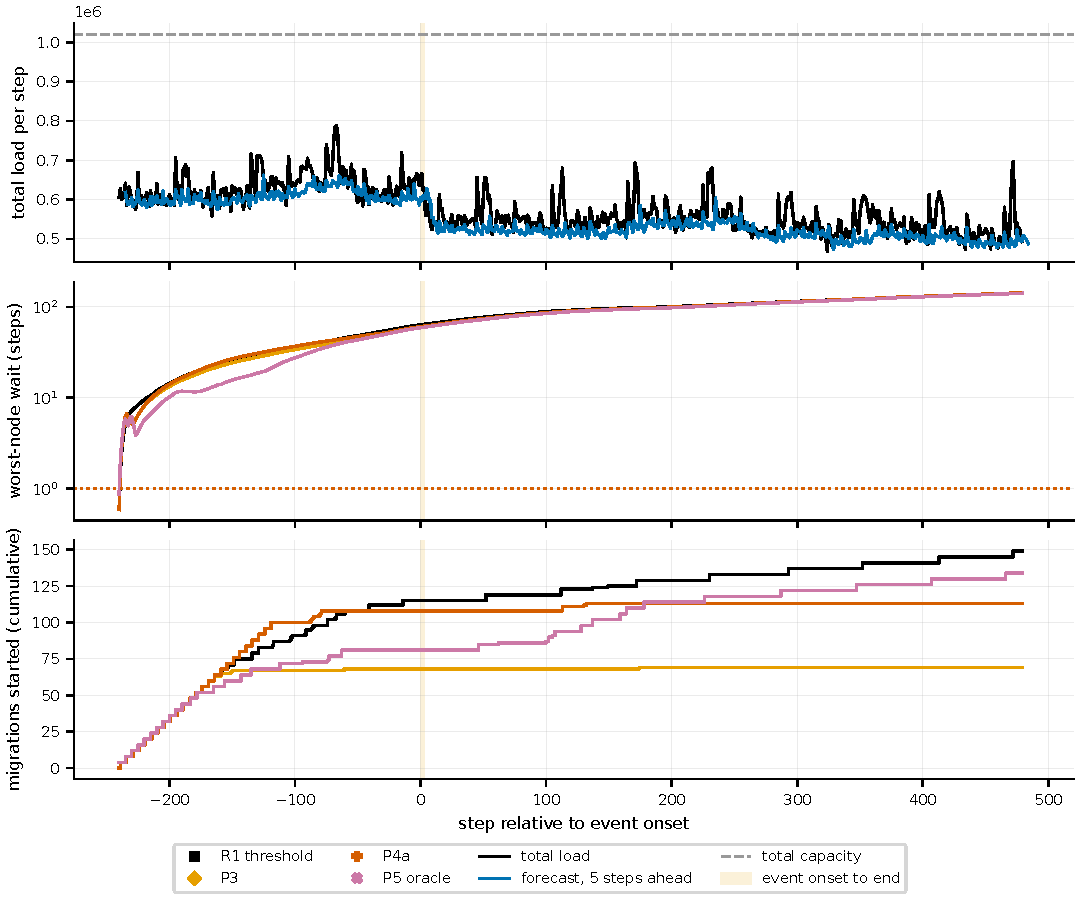
\includegraphics[width=\linewidth]{assets/figures/fa2_episode_D1.pdf}
\caption{FA2 and review Figure 3. Regenerated flash-crowd episode on D1: event D1-5320 (peak 1044), replicate 23. One replicate selected by a rule fixed beforehand, not an average, no interval. Rule: among the 30 sampled abrupt evaluation events of the default cell (m 5, headroom 1.6) the event with the median peak (lower middle on an even count, ties by event id), with the replicate index it has in the frozen rows. Top: total offered load per step, total node capacity and the point forecast of the P4 forecaster (lightgbm), summed over partitions, for the horizon of 5 steps (the default migration duration), the forecast made at step i drawn at its target step i + 5; P3 and P4a act on forecasts of this forecaster and P4a adds an interval margin that is not drawn; the shaded span runs from event onset to end. Middle: worst-node wait proxy in steps (symlog axis, SLO threshold 1 dotted). Bottom: migrations started, cumulative. Policies R1 (P1), P3 (forecaster of P4), P4a, P5. The regenerated damage and number of moves of every drawn policy equal the frozen rows (damage: R1 threshold 12.4552; P3 18.129; P4a 14.3718; P5 oracle 11.8953). Window 720 steps of 60 s, master\_seed 42. Sources: results\_frozen Must rows (P1, P3, P5) and Q1 AA6 rows (P4a), regenerated with the frozen code and configs; table of the comparison: figures/fa2\_episode\_check.csv.}\label{fig:fa2_episode_d1}
\end{figure}

% generated by build_assets.py from the recorded PDF and caption; do not edit
\begin{figure}[tbp]
\centering
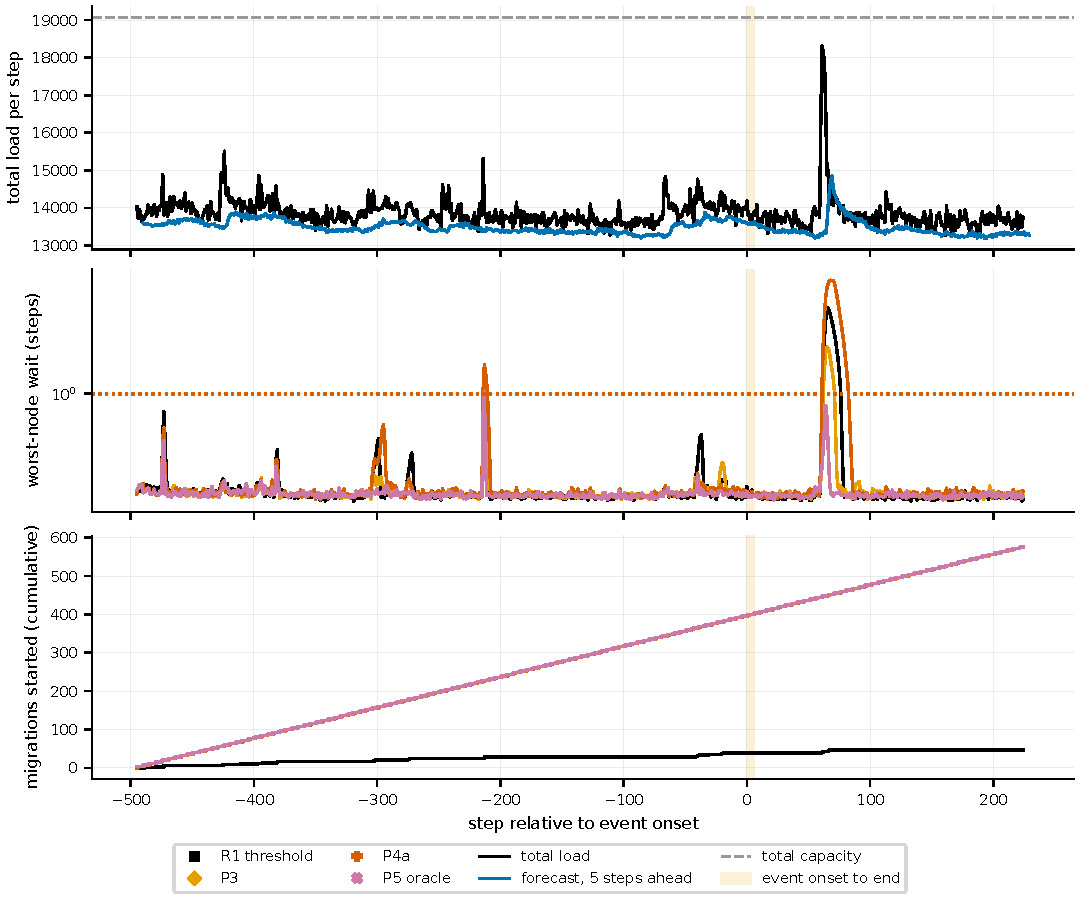
\includegraphics[width=\linewidth]{assets/figures/fa2_episode_D2.pdf}
\caption{FA2 and review Figure 3. Regenerated flash-crowd episode on D2: event D2-122 (peak 175), replicate 22. One replicate selected by a rule fixed beforehand, not an average, no interval. Rule: among the 30 sampled abrupt evaluation events of the default cell (m 5, headroom 1.6) the event with the median peak (lower middle on an even count, ties by event id), with the replicate index it has in the frozen rows. Top: total offered load per step, total node capacity and the point forecast of the P4 forecaster (lightgbm), summed over partitions, for the horizon of 5 steps (the default migration duration), the forecast made at step i drawn at its target step i + 5; P3 and P4a act on forecasts of this forecaster and P4a adds an interval margin that is not drawn; the shaded span runs from event onset to end. Middle: worst-node wait proxy in steps (symlog axis, SLO threshold 1 dotted). Bottom: migrations started, cumulative. Policies R1 (P1), P3 (forecaster of P4), P4a, P5. The regenerated damage and number of moves of every drawn policy equal the frozen rows (damage: R1 threshold 0.00330456; P3 0.00102777; P4a 0.00609227; P5 oracle 2.76524e-06). Window 720 steps of 10 s, master\_seed 42. Sources: results\_frozen Must rows (P1, P3, P5) and Q1 AA6 rows (P4a), regenerated with the frozen code and configs; table of the comparison: figures/fa2\_episode\_check.csv.}\label{fig:fa2_episode_d2}
\end{figure}

% generated by build_assets.py from the recorded PDF and caption; do not edit
\begin{figure}[tbp]
\centering
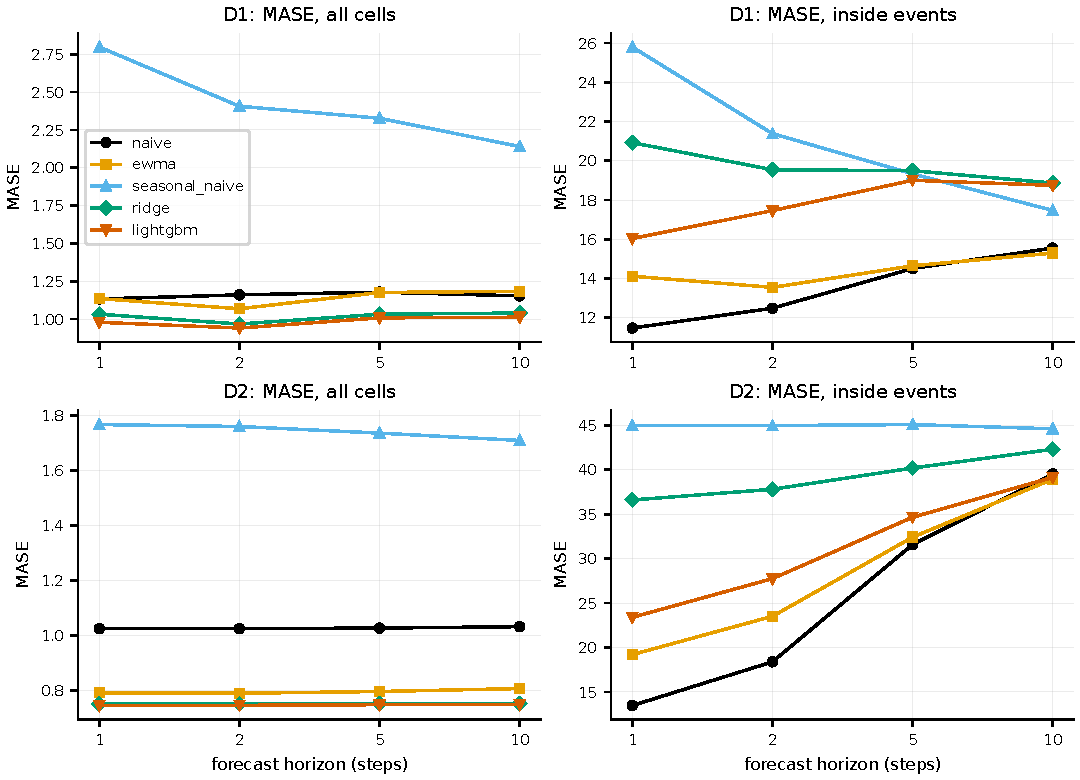
\includegraphics[width=\linewidth]{assets/figures/fa3_forecast_accuracy.pdf}
\caption{FA3. Forecast accuracy on the evaluation split, MASE over all cells and inside events, by forecaster and horizon, per dataset (D1, D2). Values are pooled point estimates from tables/forecast\_accuracy.csv; no interval is drawn because the table holds none. MASE is scaled by the training-prefix naive error, so 1 equals that scale. Source rows are rolling-refit forecasts; the stride-4 Chronos subset is not drawn (see tables/forecast\_accuracy\_chronos.csv). Seed: forecasts are deterministic given the stored tables (master seed 42).}\label{fig:fa3_forecast_accuracy}
\end{figure}

% generated by build_assets.py from the recorded PDF and caption; do not edit
\begin{figure}[tbp]
\centering
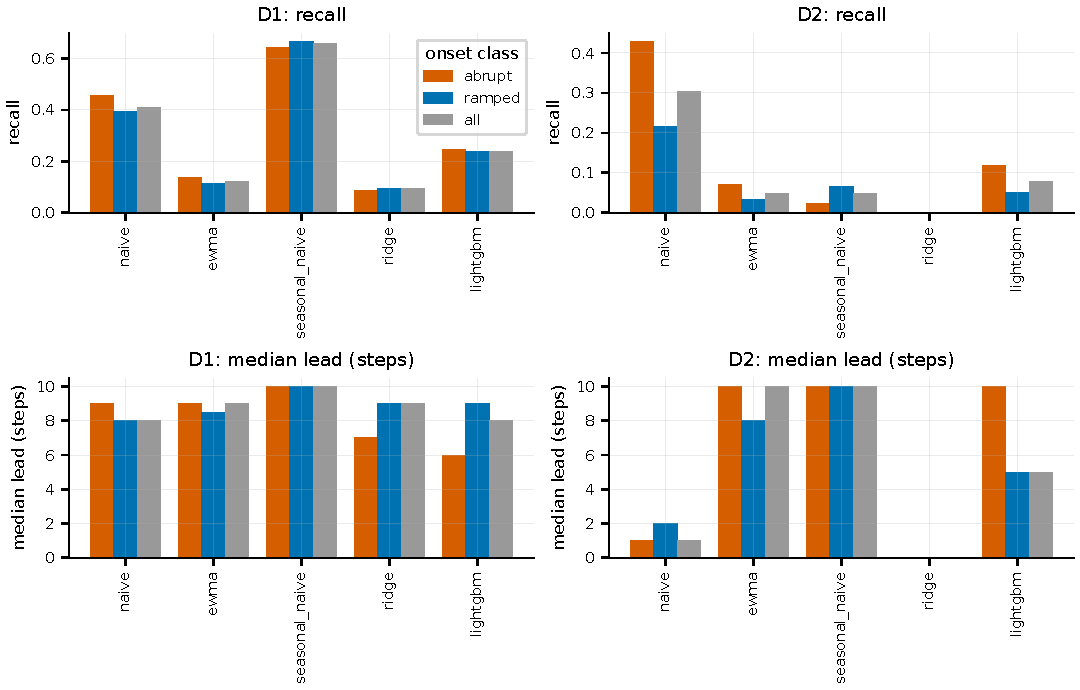
\includegraphics[width=\linewidth]{assets/figures/fa4_early_warning.pdf}
\caption{FA4. Early warning on the evaluation split: recall and median lead time (steps) of each forecaster by onset class, per dataset. Pooled point values from tables/forecast\_accuracy\_early\_warning.csv, no interval in the table. Events per class (naive row, after exclusions; other forecasters differ by the excluded events listed in the table): D1 all 3679; D1 abrupt 957; D1 ramped 2722; D2 all 102; D2 abrupt 42; D2 ramped 60. A missing bar means the value is undefined (no alarm raised). Precision is in the table and is not drawn.}\label{fig:fa4_early_warning}
\end{figure}

% generated by build_assets.py from the recorded PDF and caption; do not edit
\begin{figure}[tbp]
\centering
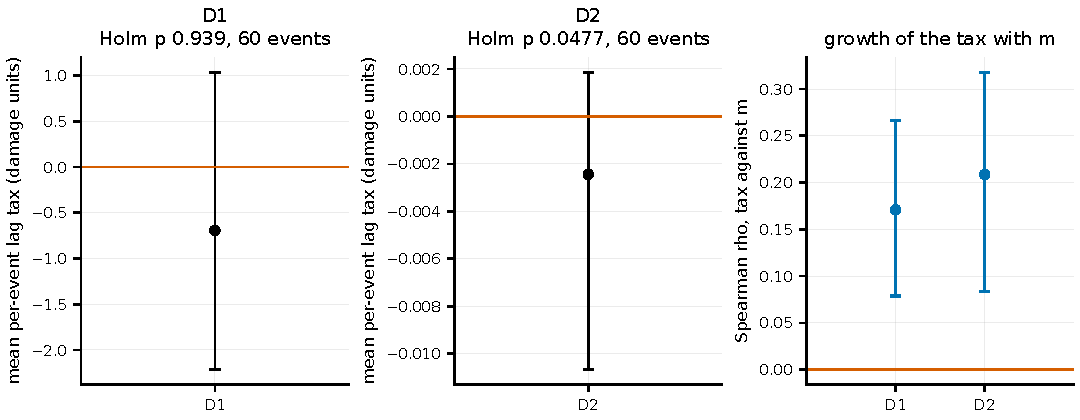
\includegraphics[width=\linewidth]{assets/figures/fa5_lag_tax.pdf}
\caption{FA5. Lag tax (reactive minus oracle damage) per event at the default m and headroom: mean with its 95\% BCa interval over events (9999 resamples, master seed 42) (left, per dataset, own axis because D1 and D2 damage scales differ), and Spearman rho of tax against m (right). Zero line marks no tax. 60 events per dataset; labels and Holm-adjusted p values are those of tables/c1\_lag\_tax.csv (family F1, 4 p values). Hypothesis labels are in the ledger.}\label{fig:fa5_lag_tax}
\end{figure}

% generated by build_assets.py from the recorded PDF and caption; do not edit
\begin{figure}[tbp]
\centering
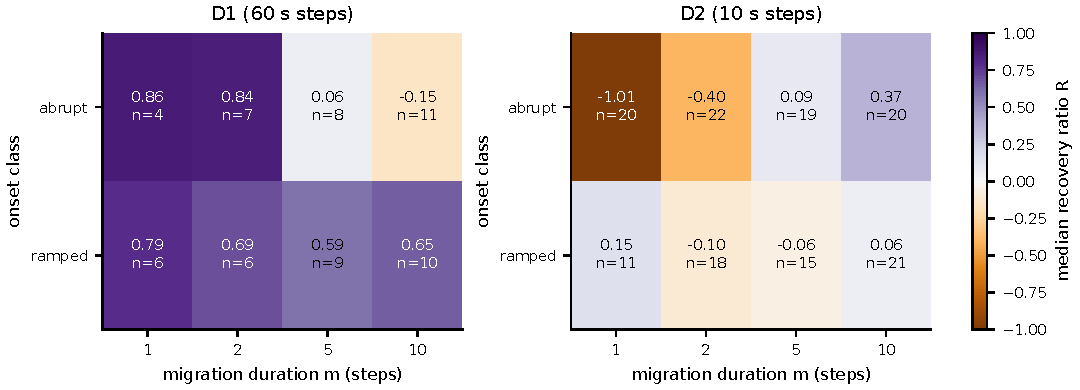
\includegraphics[width=\linewidth]{assets/figures/fa6_regime_must.pdf}
\caption{FA6b. Headline regime map on the real traces: median recovery ratio R of P3\_lightgbm by migration duration m and onset class at headroom 1.6, per dataset. Cell text is the median R over events with R defined and the number n of those events; blank cells have no event with R defined. Colour clipped to -1 to 1. Intervals and the share of replicates with R defined are in tables/regime\_map\_must.csv. Datasets are not pooled.}\label{fig:fa6_regime_must}
\end{figure}

% generated by build_assets.py from the recorded PDF and caption; do not edit
\begin{figure}[tbp]
\centering
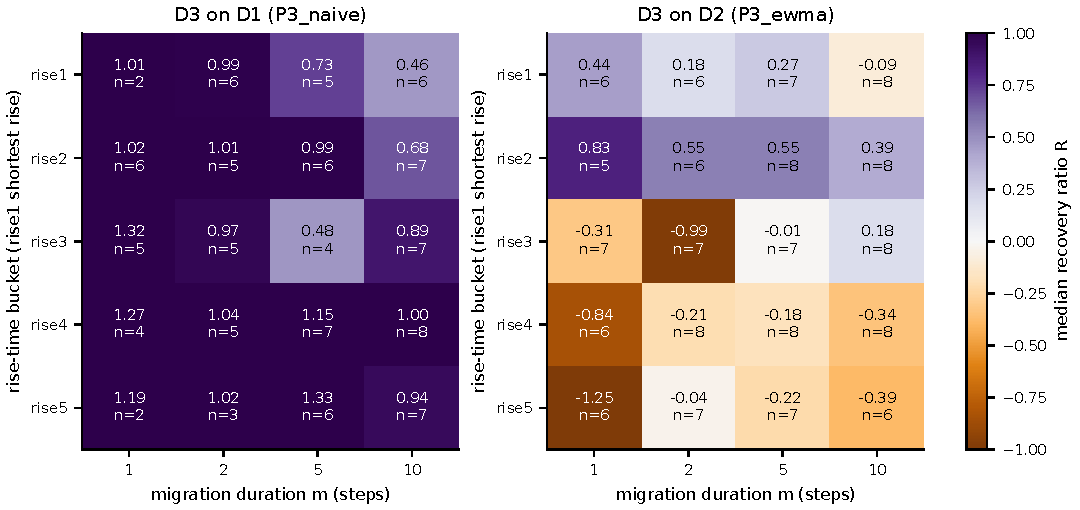
\includegraphics[width=\linewidth]{assets/figures/fa6_regime_q2.pdf}
\caption{FA6a. Measured lag-tax recovery ratio R across migration duration m (x) and flash-crowd rise-time bucket (y), headroom 1.6, injected-event data D3 on D1 and on D2 (forecast policy: P3\_ewma/P3\_naive). Cell text is the median R over events with R defined and the number n of those events (of 8 events per bucket); blank cells have no event with R defined. Colour is clipped to the range -1 to 1, the printed value is not clipped. R is defined only where the lag tax is at least the registered share of the reactive damage. Every cell rests on few events (flag in tables/regime\_map\_q2.csv); intervals are in the table. Datasets are not pooled.}\label{fig:fa6_regime_q2}
\end{figure}

% generated by build_assets.py from the recorded PDF and caption; do not edit
\begin{figure}[tbp]
\centering
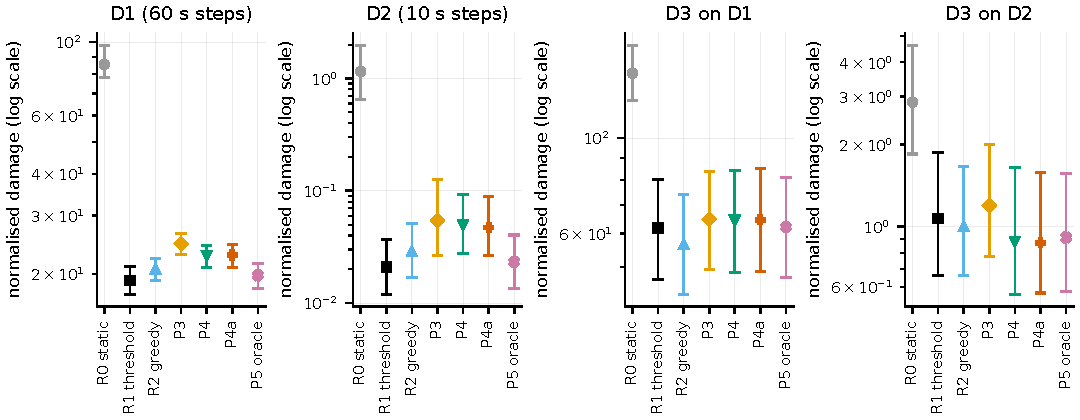
\includegraphics[width=\linewidth]{assets/figures/fa7_damage.pdf}
\caption{FA7a. Overall performance of the seven placement policies: mean per-event normalised damage with its 95\% BCa interval over events (9999 resamples, master seed 42), per dataset (log y axis, each panel its own scale; datasets are not pooled because D1 damage is about 20 and D2 about 0.02). R0, R1 and R2 are P0, P1 and P2. Events per dataset: D1 60; D2 60; D1\_D3 40; D2\_D3 40. Default m and headroom, 30 replicates per event, tables/rt\_policy\_metrics.csv (descriptive, not pre-registered).}\label{fig:fa7_damage}
\end{figure}

% generated by build_assets.py from the recorded PDF and caption; do not edit
\begin{figure}[tbp]
\centering
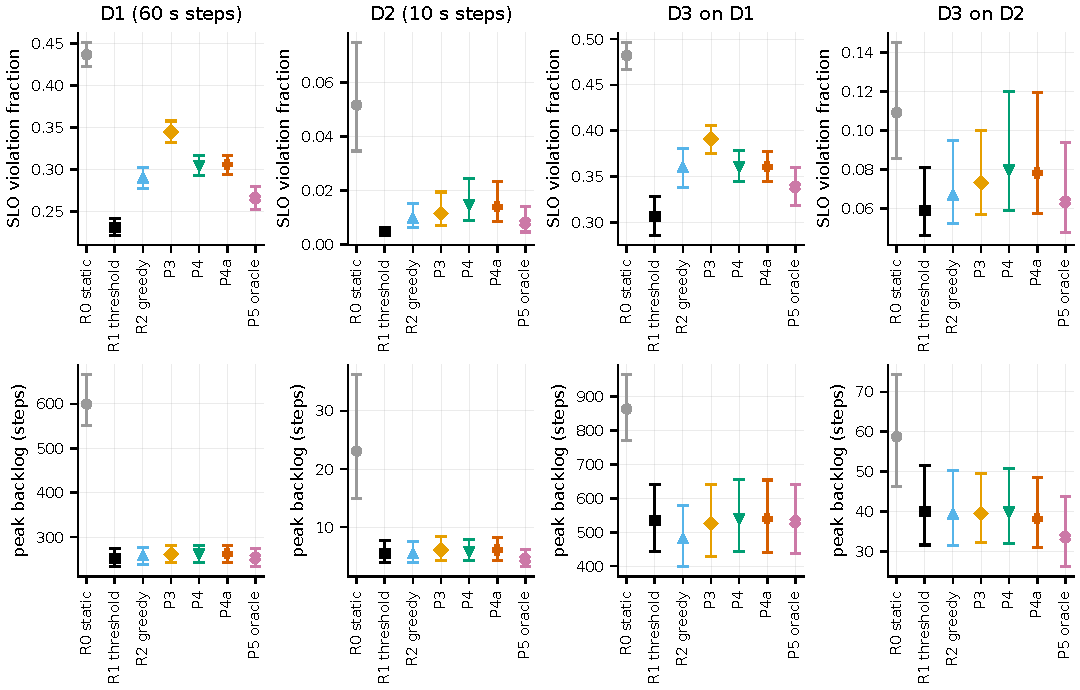
\includegraphics[width=\linewidth]{assets/figures/fa7_violation_backlog.pdf}
\caption{FA7b. SLO violation fraction (top) and peak backlog in steps (bottom) for the seven policies, per dataset: mean per-event value with its 95\% BCa interval over events (9999 resamples, master seed 42). R0, R1, R2 are P0, P1, P2. Events per dataset: D1 60; D2 60; D1\_D3 40; D2\_D3 40. Default m and headroom; tables/rt\_policy\_metrics.csv (descriptive, not pre-registered).}\label{fig:fa7_violation_backlog}
\end{figure}

% generated by build_assets.py from the recorded PDF and caption; do not edit
\begin{figure}[tbp]
\centering
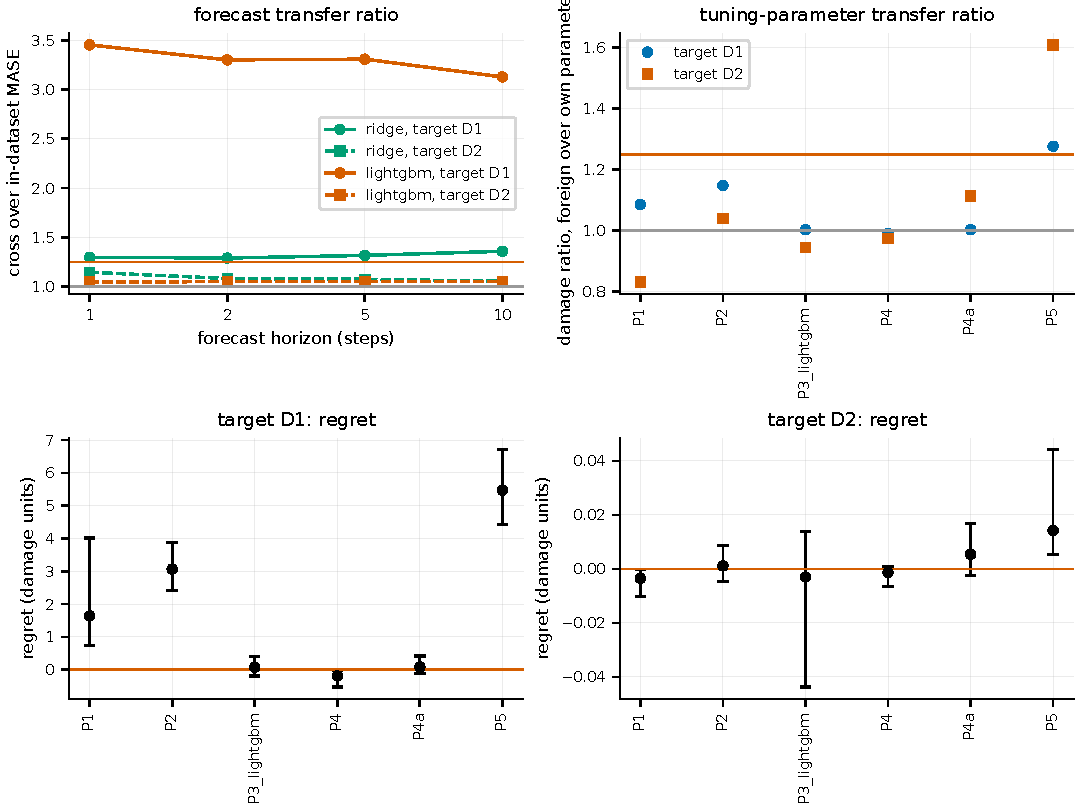
\includegraphics[width=\linewidth]{assets/figures/fa8_transfer.pdf}
\caption{FA8. Cross-dataset transfer. Top left: forecast transfer ratio (fixed model fitted on the source training prefix, scored on the target, over the same protocol in-dataset), ridge and lightgbm, by horizon and target. Top right: tuning-parameter transfer ratio of mean per-event damage, foreign over own parameters, per policy and target. Lines: 1 (grey) and the registered threshold 1.25 (orange). Bottom: regret (foreign minus own mean damage) with 95\% BCa interval over events (9999 resamples, master seed 42), per target on its own damage scale. Source: tables/c5\_transfer\_detail.csv; ratios have no interval in the table.}\label{fig:fa8_transfer}
\end{figure}

% generated by build_assets.py from the recorded PDF and caption; do not edit
\begin{figure}[tbp]
\centering
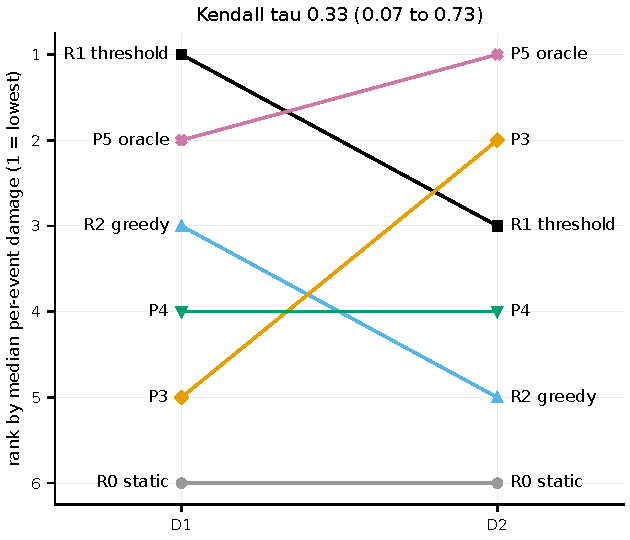
\includegraphics[width=\linewidth]{assets/figures/fa9_ranking.pdf}
\caption{FA9. Policy ranking on D1 and D2 by median per-event damage (60 events on D1, 60 on D2), rank 1 is the lowest damage. R0, R1, R2 are P0, P1, P2. Kendall tau between the two rankings, tau and its percentile bootstrap interval are in the title (6 policies, threshold 0.6 in tables/c6\_ranking\_tau.csv). Source: tables/c6\_ranking.csv.}\label{fig:fa9_ranking}
\end{figure}

% generated by build_assets.py from the recorded PDF and caption; do not edit
\begin{figure}[tbp]
\centering
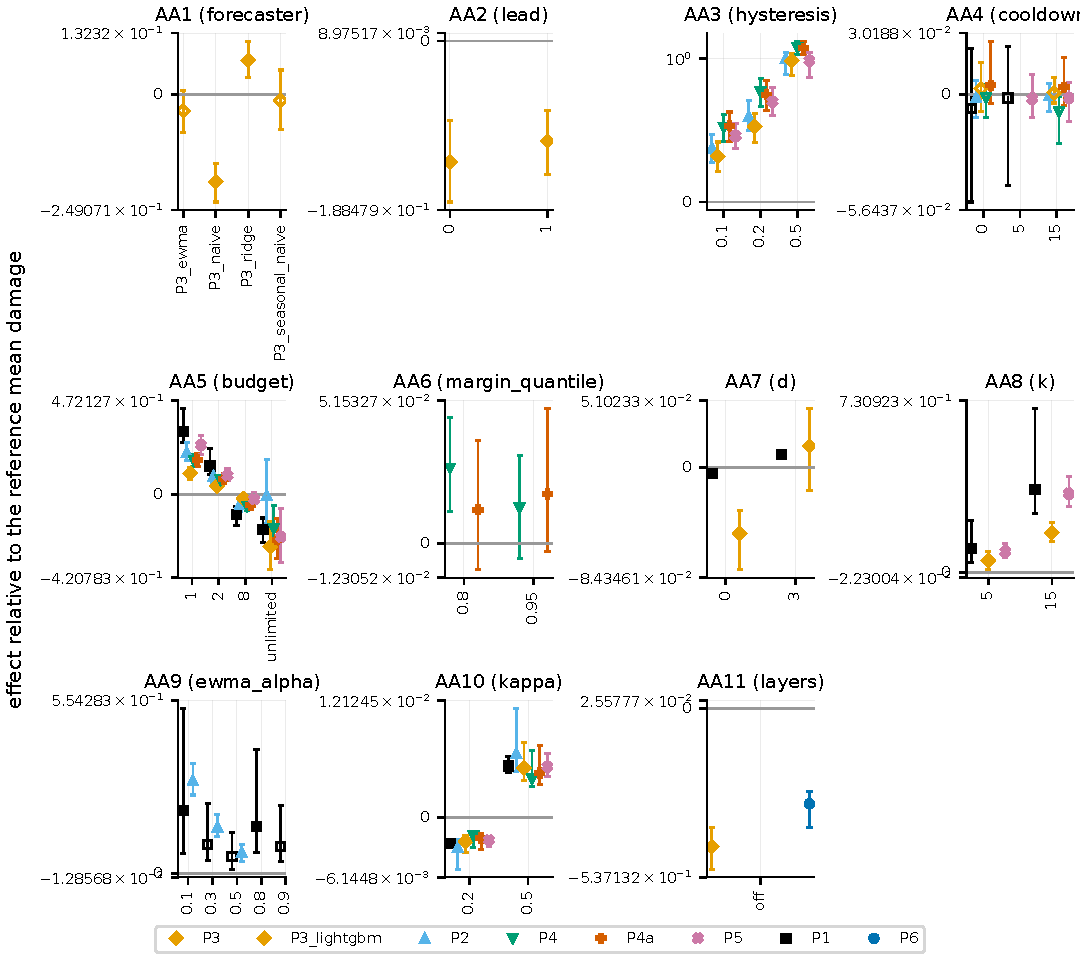
\includegraphics[width=\linewidth]{assets/figures/fa10_ablations_D1.pdf}
\caption{FA10 (D1). Ablation effects on mean per-event damage, level minus reference, as a multiple of the reference mean (symlog axis; 0 means no change, 1 means +100 percent), per ablation AA1 to AA11 and policy, with 95\% BCa interval over events (9999 resamples, master seed 42) over 60 events scaled by the reference mean. Filled markers: Holm-adjusted p below the registered alpha within the ablation; open markers: not. One factor at a time, levels not re-tuned; interactions untested; AA13, XA6 and FA16 were not completed. Source: tables/aa\_ablations.csv (descriptive, no hypothesis label).}\label{fig:fa10_ablations_d1}
\end{figure}

% generated by build_assets.py from the recorded PDF and caption; do not edit
\begin{figure}[tbp]
\centering
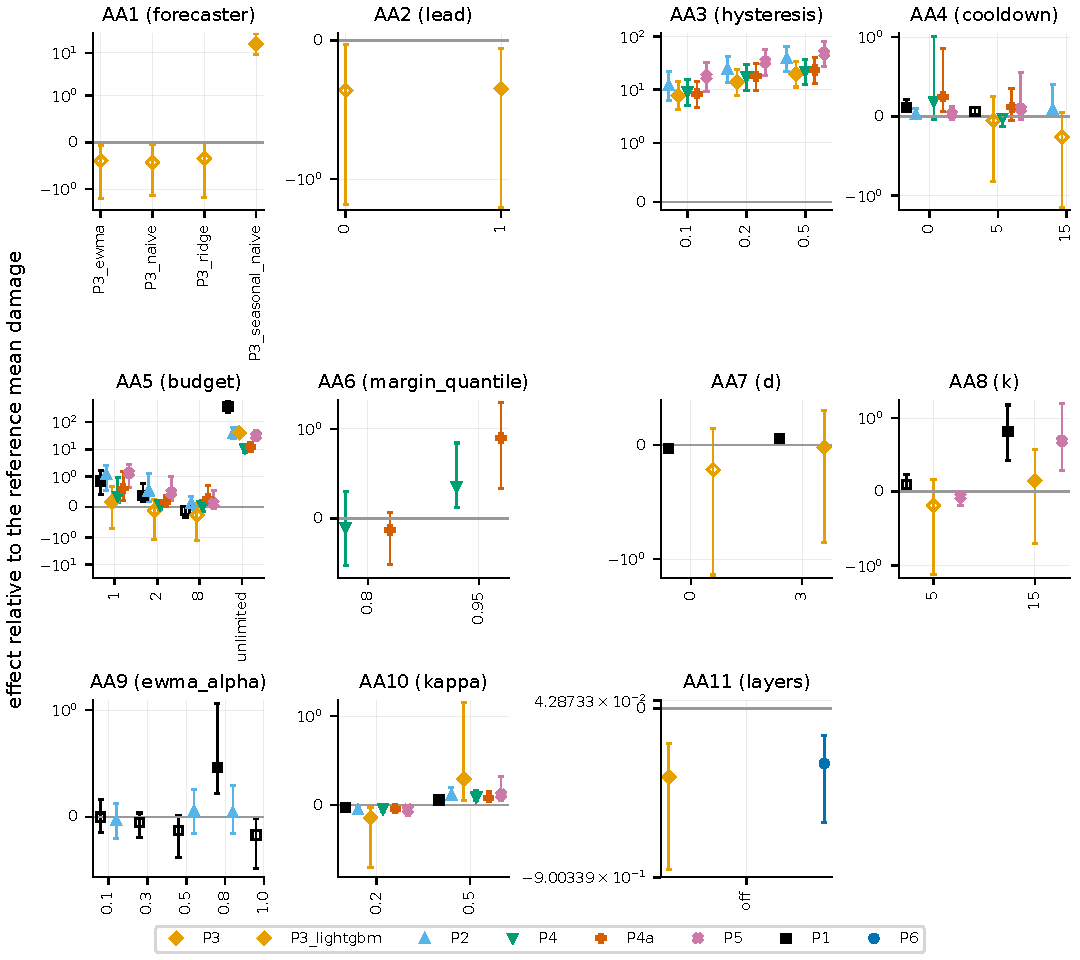
\includegraphics[width=\linewidth]{assets/figures/fa10_ablations_D2.pdf}
\caption{FA10 (D2). Ablation effects on mean per-event damage, level minus reference, as a multiple of the reference mean (symlog axis; 0 means no change, 1 means +100 percent), per ablation AA1 to AA11 and policy, with 95\% BCa interval over events (9999 resamples, master seed 42) over 60 events scaled by the reference mean. Filled markers: Holm-adjusted p below the registered alpha within the ablation; open markers: not. One factor at a time, levels not re-tuned; interactions untested; AA13, XA6 and FA16 were not completed. Source: tables/aa\_ablations.csv (descriptive, no hypothesis label).}\label{fig:fa10_ablations_d2}
\end{figure}

% generated by build_assets.py from the recorded PDF and caption; do not edit
\begin{figure}[tbp]
\centering
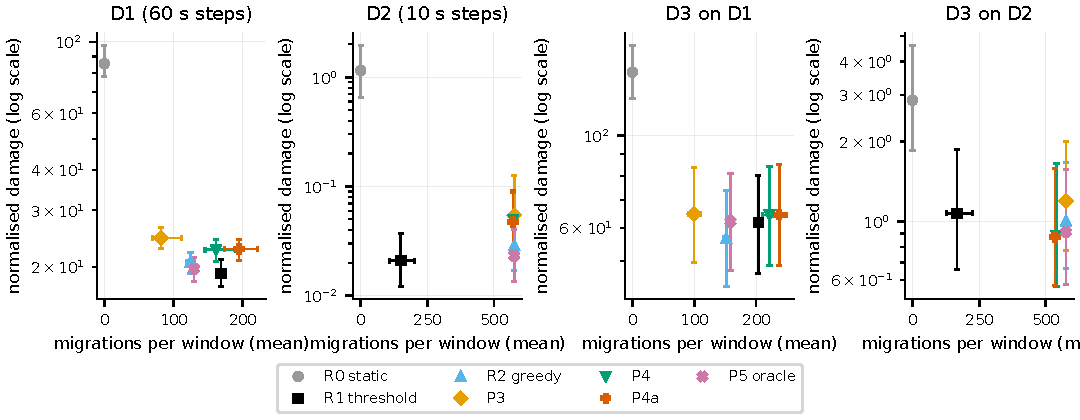
\includegraphics[width=\linewidth]{assets/figures/fa11_damage_moves.pdf}
\caption{FA11. Damage against migration count per policy, per dataset (each panel its own damage scale): mean per-event value with its 95\% BCa interval over events (9999 resamples, master seed 42) on both axes. R0, R1, R2 are P0, P1, P2; R0 never migrates. Events per dataset: D1 60; D2 60; D1\_D3 40; D2\_D3 40. Default m and headroom; tables/rt\_policy\_metrics.csv (descriptive, not pre-registered).}\label{fig:fa11_damage_moves}
\end{figure}

% generated by build_assets.py from the recorded PDF and caption; do not edit
\begin{figure}[tbp]
\centering
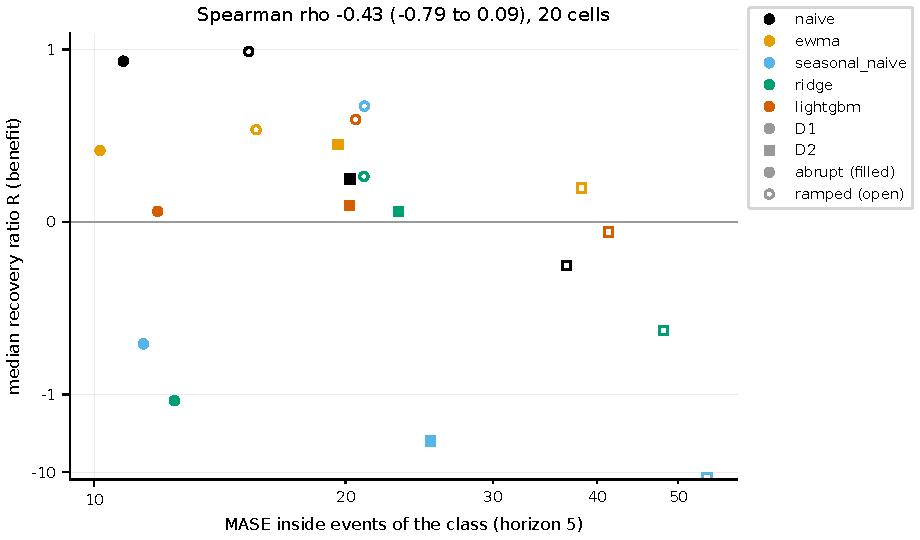
\includegraphics[width=\linewidth]{assets/figures/fa12_mase_benefit.pdf}
\caption{FA12. Forecast accuracy against control benefit: one point per cell (forecaster, dataset, onset class), x is the MASE inside events of that class at the horizon nearest m plus d, y is the cell median recovery ratio R. Circles: D1, squares: D2; filled: abrupt, open: ramped. Spearman rho with its 95\% BCa interval over events (9999 resamples, master seed 42) over cells is in the title (exploratory p 0.0594); cell benefits rest on the events with R defined (8 to 19 per cell, tables/c4\_accuracy\_benefit\_cells.csv). Symlog y axis.}\label{fig:fa12_mase_benefit}
\end{figure}

% generated by build_assets.py from the recorded PDF and caption; do not edit
\begin{figure}[tbp]
\centering
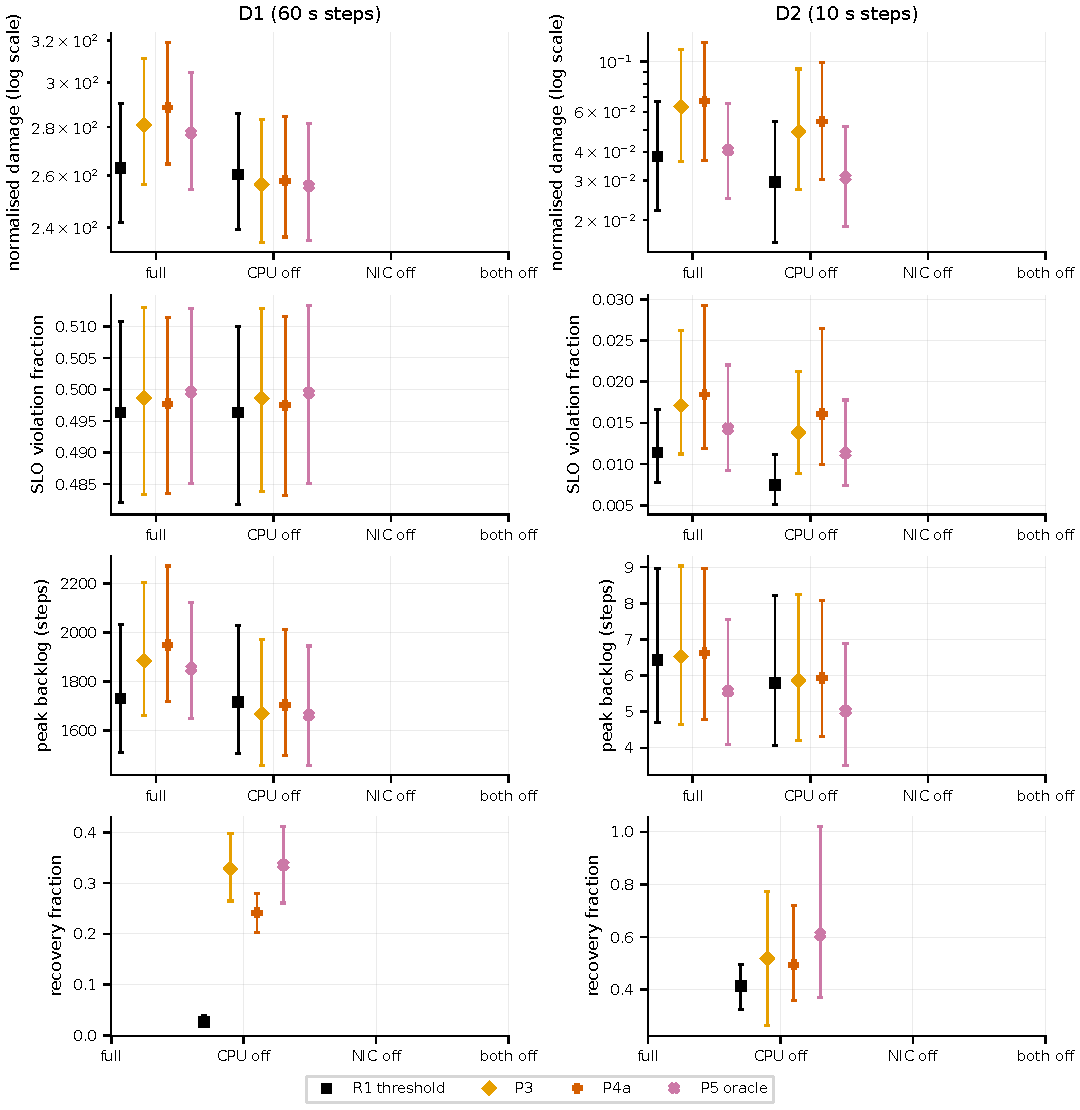
\includegraphics[width=\linewidth]{assets/figures/fa13_contention.pdf}
\caption{FA13. Contention ablation (RV1) in the coupled model, per dataset (each panel its own scale): mean per-event damage (log scale), SLO violation fraction and peak backlog with their 95\% BCa interval over events (9999 resamples, master seed 42), and the recovery fraction of tables/rv1\_contention.csv (bottom row; blank where it is undefined, which includes the full model, the reference). Levels: full model, CPU contention off, NIC contention off, both off. The constant-m control mode is in the tables and not drawn. Events per dataset: D1 60; D2 60. Tables: tables/rt\_rv1\_metrics.csv (descriptive, not pre-registered) and tables/rv1\_contention.csv.}\label{fig:fa13_contention}
\end{figure}

% generated by build_assets.py from the recorded PDF and caption; do not edit
\begin{figure}[tbp]
\centering
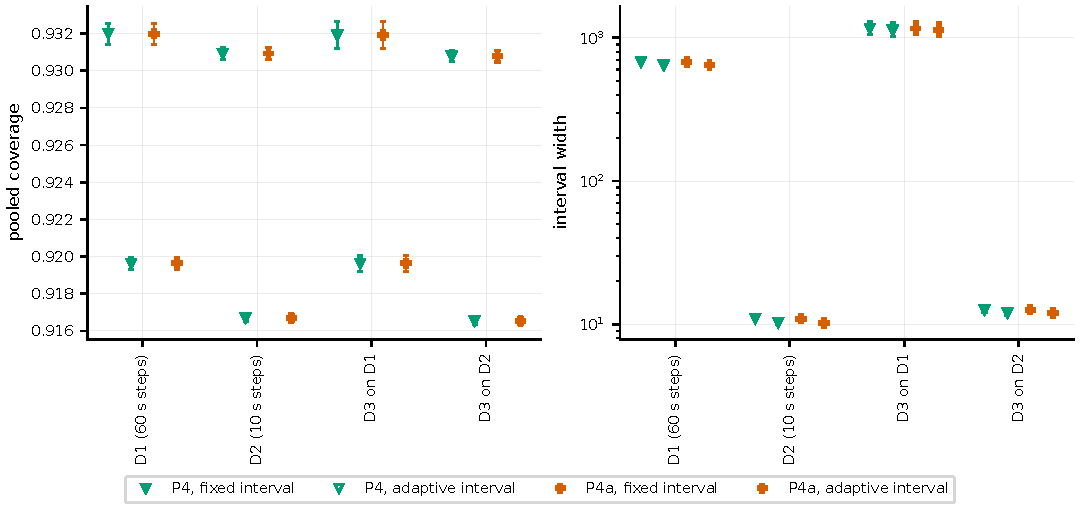
\includegraphics[width=\linewidth]{assets/figures/fa14_conformal_logging.pdf}
\caption{FA14. Conformal interval logging (RV4): pooled coverage (left) and interval width (right, log scale) of the fixed and the adaptive interval, for P4 and P4a, per dataset (widths are not comparable across datasets). Filled markers: fixed interval; open: adaptive. Mean with its 95\% BCa interval over events (9999 resamples, master seed 42). The table holds pooled values, so there is no time axis; the adaptive level (alpha), the point error and the trigger counts are in the table and not drawn. Events per dataset: D1 60; D2 60; D1\_D3 40; D2\_D3 40. Source: tables/rv4\_logging.csv.}\label{fig:fa14_conformal_logging}
\end{figure}

% generated by build_assets.py from the recorded PDF and caption; do not edit
\begin{figure}[tbp]
\centering
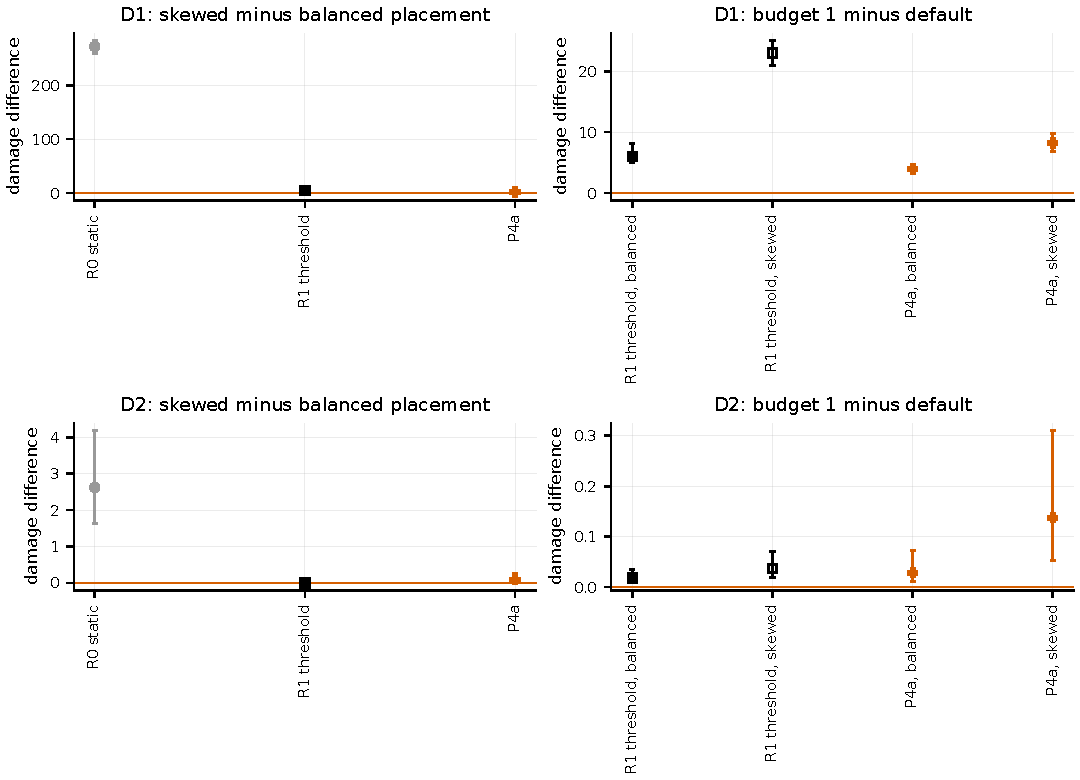
\includegraphics[width=\linewidth]{assets/figures/fa15_placement_budget.pdf}
\caption{FA15. Placement and migration budget (RV2, RV3), per dataset (each panel its own damage scale). Left: mean per-event damage under skewed placement minus balanced placement, for R0, R1 and P4a. Right: mean per-event damage with migration budget 1 minus the default budget, for R1 and P4a, under balanced placement (filled) and skewed placement (open). Mean difference with its 95\% BCa interval over events (9999 resamples, master seed 42); zero line marks no difference. R0, R1 are P0, P1. Events per dataset: D1 60; D2 60. Sources: tables/rv2\_placement.csv and tables/rv3\_budget.csv. Review figure 10 asked for the throttled policy; the recorded RV3 rows hold the budget-1 contrast, which is what is drawn.}\label{fig:fa15_placement_budget}
\end{figure}

 once
% needs: booktabs, longtable, adjustbox, graphicx
% generated by build_assets.py from the recorded CSV; do not edit
\begin{table}[tbp]
\centering
\scriptsize
\caption{Datasets}\label{tab:ta1}
\adjustbox{max width=\linewidth}{%
\begin{tabular}{llrrrrrrrrrrrl}
\toprule
dataset & role & step seconds & n steps & span days & n partitions & train end & tune end & eval steps & n events & events eval abrupt & events eval ramped & events eval all & bytes provenance \\
\midrule
D1 & primary real trace & 60 & 10080 & 7 & 512 & 2880 & 4320 & 5760 & 6482 & 964 & 2743 & 0 & assumed \\
D2 & second real trace & 10 & 18508 & 2.142 & 512 & 4627 & 7403 & 11105 & 177 & 42 & 60 & 0 & real \\
D1\_D3 & D1 with injected events & 60 & 10080 & 7 & 512 & 2880 & 4320 & 5760 & 40 & 0 & 0 & 40 & assumed \\
D2\_D3 & D2 with injected events & 10 & 18508 & 2.142 & 512 & 4627 & 7403 & 11105 & 40 & 0 & 0 & 40 & real \\
\bottomrule
\end{tabular}}
\end{table}

% generated by build_assets.py from the recorded CSV; do not edit
{\scriptsize
\setlength{\tabcolsep}{3pt}
\begin{longtable}{lllll}
\caption{Parameters with real, assumed or design tag}\label{tab:ta2}\\
\toprule
key & parent & value & real or assumed & justification \\
\midrule
\endfirsthead
\toprule
key & parent & value & real or assumed & justification \\
\midrule
\endhead
\bottomrule
\endfoot
enabled & layers & false & design & n/a \\
n\_partitions & n/a & 512 & real & n/a \\
n\_nodes & n/a & 16 & real & n/a \\
headroom & n/a & 1.6 & assumed & n/a \\
slo\_threshold & n/a & 1 & design & n/a \\
window\_steps & n/a & 720 & design & n/a \\
step\_seconds & n/a & 60 & real & n/a \\
migration\_steps\_m0 & n/a & 5 & assumed & n/a \\
migration\_overhead\_kappa & n/a & 0.3 & assumed & n/a \\
migration\_budget\_B & n/a & 4 & design & n/a \\
monitor\_delay\_d & n/a & 1 & design & n/a \\
decision\_interval\_k & n/a & 1 & design & n/a \\
horizons & n/a & [1, 2, 5, 10] & design & n/a \\
refit\_interval & n/a & 360 & assumed & n/a \\
seasonal\_period & n/a & 1440 & real & n/a \\
tuning\_budget & n/a & 36 & design & n/a \\
tune\_plateau\_tol & n/a & 0.05 & assumed & n/a \\
ewma\_alpha\_grid & n/a & [0.1, 0.3, 0.5, 0.8] & design & n/a \\
theta\_hi\_grid & n/a & [0.8, 0.9, 1.0] & design & n/a \\
cooldown\_grid & n/a & [0, 5, 15] & design & n/a \\
hysteresis\_grid & n/a & [0.0, 0.1, 0.2, 0.5] & design & n/a \\
oracle\_window\_grid & n/a & [1, 5, 10] & design & n/a \\
margin\_quantile & n/a & 0.9 & design & n/a \\
replicates\_per\_cell & n/a & 30 & design & n/a \\
min\_replicates & n/a & 30 & design & n/a \\
m\_levels & n/a & [1, 2, 5, 10] & design & n/a \\
headroom\_levels & n/a & [1.3, 1.6, 2.0] & design & n/a \\
pilot\_replicates & n/a & 5 & design & n/a \\
oracle\_check\_events & n/a & 100 & design & n/a \\
n\_boot & n/a & 9999 & design & n/a \\
ci\_level & n/a & 0.95 & design & n/a \\
r & n/a & 5 & design & n/a \\
W\_b & n/a & 60 & design & n/a \\
s & n/a & 3 & design & n/a \\
eps & n/a & 0.001 & design & n/a \\
rise\_lo & n/a & 0.1 & design & n/a \\
rise\_hi & n/a & 0.9 & design & n/a \\
simplex\_step & n/a & 0.1 & design & n/a \\
min\_events & n/a & 24 & design & n/a \\
min\_lag\_tax\_share & n/a & 0.05 & design & n/a \\
capacity\_jitter\_frac & n/a & 0.1 & assumed & n/a \\
wasted\_move\_window & n/a & 10 & design & n/a \\
inject\_tolerance & n/a & 5 & design & n/a \\
injection\_amplitude\_min & n/a & 10 & assumed & n/a \\
injection\_amplitude\_max & n/a & 100 & assumed & n/a \\
injection\_rise\_min & n/a & 2 & assumed & n/a \\
injection\_rise\_max & n/a & 10 & assumed & n/a \\
injection\_dur\_min & n/a & 10 & assumed & n/a \\
injection\_dur\_max & n/a & 50 & assumed & n/a \\
cpu\_cores & n/a & 8 & real & n/a \\
h\_net & n/a & 2 & assumed & n/a \\
rho & n/a & 0.25 & assumed & n/a \\
sigma\_size & n/a & 0.5 & assumed & n/a \\
phi & n/a & 1 & assumed & n/a \\
master\_seed & n/a & 42 & design & n/a \\
hash\_seed & n/a & 'seed1' & design & n/a \\
reserved\_cores & n/a & 1 & design & n/a \\
workers & n/a & 7 & design & n/a \\
compute\_budget\_core\_hours & n/a & 288 & real & n/a \\
runner\_stall\_minutes & n/a & 30 & design & n/a \\
cleanroom\_stride & n/a & 1 & design & n/a \\
d2\_max\_gb & n/a & 2 & real & n/a \\
azure\_days & n/a & 7 & real & n/a \\
azure\_skip\_cols & n/a & 4 & real & n/a \\
d2\_min\_cols & n/a & 4 & real & n/a \\
c0 & n/a & 1 & assumed & n/a \\
c1 & n/a & 0 & assumed & n/a \\
azure\_mins\_per\_day & n/a & 1440 & real & n/a \\
data\_root & n/a & 'data' & real & n/a \\
ridge\_alpha & n/a & [0.1, 1.0, 10.0] & design & n/a \\
lightgbm\_leaves & n/a & [15, 31, 63] & design & n/a \\
gamma & n/a & 0.005 & design & ACI step size, the value used in the A15 experiments (Gibbs and Candes 2021, Sec 2.1), not tuned here (A26) \\
a\_min & n/a & 0.01 & assumed & n/a \\
a\_max & n/a & 0.2 & assumed & n/a \\
residual\_window & n/a & 100 & design & n/a \\
psi\_grid & n/a & [0.1, 0.2, 0.5] & design & n/a \\
io\_chunk\_bytes & compute & 65536 & design & n/a \\
snapshots & paths & 'snapshots' & design & n/a \\
default\_tag & snapshot & 'prereg-v1' & design & n/a \\
tag\_pattern & snapshot & '[a-zA-Z0-9\_-]+' & design & n/a \\
sources & snapshot & ['src', 'scripts', 'configs'] & design & n/a \\
ignore\_patterns & snapshot & ['*.pyc', '\_\_pycache\_\_'] & design & n/a \\
manifest\_name & snapshot & 'manifest.json' & design & n/a \\
raw\_dirname & n/a & 'raw' & design & n/a \\
azure\_dirname & n/a & 'azure2019' & design & n/a \\
twitter\_dirname & n/a & 'twitter' & design & n/a \\
processed\_dirname & n/a & 'processed' & design & n/a \\
logs\_dirname & n/a & 'logs' & design & n/a \\
amendments\_file & n/a & 'AMENDMENTS.md' & design & n/a \\
d2\_file & n/a & 'cluster53.sort.zst' & real & n/a \\
azure\_invocation\_pattern & n/a & 'invocations\_per\_function\_md.anon.d\{day:02d\}.csv' & real & n/a \\
azure\_duration\_pattern & n/a & 'function\_durations\_percentiles.anon.d\{day:02d\}.csv' & real & n/a \\
azure\_memory\_pattern & n/a & 'app\_memory\_percentiles.anon.d\{day:02d\}.csv' & real & n/a \\
azure\_head\_cols & n/a & ['HashOwner', 'HashApp', 'HashFunction', 'Trigger'] & real & n/a \\
azure\_id\_cols & n/a & ['HashOwner', 'HashApp', 'HashFunction'] & real & n/a \\
azure\_dur\_avg\_col & n/a & 'Average' & real & n/a \\
azure\_dur\_count\_col & n/a & 'Count' & real & n/a \\
azure\_memory\_cols & n/a & ['HashOwner', 'HashApp', 'SampleCount', 'AverageAllocatedMb', 'AverageAllocatedMb\_pct1', 'AverageAllocatedMb\_pct5', 'AverageAllocatedMb\_pct25', 'AverageAllocatedMb\_pct50', 'AverageAllocatedMb\_pct75', 'AverageAllocatedMb\_pct95', 'AverageAllocatedMb\_pct99', 'AverageAllocatedMb\_pct100'] & real & n/a \\
azure\_chunk\_rows & n/a & 5000 & design & n/a \\
d2\_chunk\_rows & n/a & 2000000 & design & n/a \\
d2\_cols & n/a & ['timestamp', 'key', 'key\_size', 'value\_size', 'client', 'op', 'ttl'] & real & n/a \\
d2\_time\_col & n/a & 'timestamp' & real & n/a \\
d2\_key\_col & n/a & 'key' & real & n/a \\
d2\_ksize\_col & n/a & 'key\_size' & real & n/a \\
d2\_vsize\_col & n/a & 'value\_size' & real & n/a \\
d2\_op\_col & n/a & 'op' & real & n/a \\
d2\_step\_seconds & n/a & 10 & design & n/a \\
d1\_train\_days & n/a & 2 & design & n/a \\
d1\_tune\_days & n/a & 1 & design & n/a \\
d2\_split\_fractions & n/a & [0.25, 0.15] & design & n/a \\
key\_sep & n/a & '|' & design & n/a \\
hash\_bits & n/a & 128 & real & n/a \\
d1\_bytes\_sigma & n/a & 0.5 & assumed & n/a \\
d1\_bytes\_label & n/a & 'bytes' & design & n/a \\
demand\_fallback & n/a & 1 & assumed & n/a \\
inject\_label & n/a & 'D3' & design & n/a \\
injection\_events & n/a & 40 & design & n/a \\
injection\_hot\_min & n/a & 1 & assumed & n/a \\
injection\_hot\_max & n/a & 4 & assumed & n/a \\
wait\_quantile & n/a & 0.99 & design & n/a \\
tune\_replicates & n/a & 35 & design & n/a \\
tune\_plateau\_frac & n/a & 0.25 & design & n/a \\
seed\_bits & n/a & 32 & design & n/a \\
day\_seconds & n/a & 86400 & real & n/a \\
lookback\_L & n/a & 30 & design & n/a \\
roll\_window & n/a & 10 & design & n/a \\
forecast\_ewma\_alpha & n/a & 0.3 & design & n/a \\
origin\_stride & n/a & 4 & design & n/a \\
lgbm\_trees & n/a & 100 & design & n/a \\
lgbm\_lr & n/a & 0.1 & design & n/a \\
lgbm\_verbosity & n/a & -1 & design & n/a \\
feature\_chunk\_origins & n/a & 256 & design & n/a \\
forecaster\_names & n/a & ['naive', 'ewma', 'seasonal\_naive', 'ridge', 'lightgbm'] & design & n/a \\
warn\_ratio & n/a & 3 & design & n/a \\
warn\_baseline\_window & n/a & 60 & design & n/a \\
smape\_eps & n/a & 0.001 & design & n/a \\
forecast\_dirname & n/a & 'forecasts' & design & n/a \\
h\_net\_levels & n/a & [1.3, 2.0, 4.0] & assumed & n/a \\
phi\_levels & n/a & [1.0, 0.1, 0.01] & assumed & n/a \\
size\_label & n/a & 'part\_size' & design & n/a \\
budget\_levels & n/a & [1, 2, 8, 'unlimited'] & design & AA5 levels besides the default 4; unlimited means n\_partitions (A34) \\
margin\_levels & n/a & [0.8, 0.9, 0.95] & design & AA6 margin levels for P4 and P4a (A34) \\
lead\_levels & n/a & [0, 1] & design & AA2 steps ahead of t the policy targets besides the default m: current step 0, next step 1 (A34) \\
rise\_buckets & n/a & 5 & design & D3 rise-time buckets of equal event count (A36) \\
D1 & q2\_forecast\_variants & P3\_naive & design & 14.9053 against P4 15.8977 and P3\_ewma 15.5024 \\
D2 & q2\_forecast\_variants & P3\_ewma & design & 0.00285714 against P3\_naive 0.00480893 and P4 0.0683602 \\
interaction\_effect\_frac & n/a & 0.05 & design & minimum effect size, as a fraction of the default mean damage, for a Q1 factor to count as active in the interaction trigger (A38) \\
interaction\_min\_active & n/a & 2 & design & the interaction trigger fires for a dataset and policy when at least this many factors are active (A38) \\
skew\_hot\_share & n/a & 0.25 & design & RV2 skewed placement: share of partitions, heaviest by training-prefix mean load, packed on the hot nodes (A38) \\
skew\_hot\_nodes & n/a & 4 & design & RV2 skewed placement: number of hot nodes, the first nodes in index order (A38) \\
kappa\_levels & n/a & [0.2, 0.3, 0.5] & assumed & AA10 migration overhead levels (guide section 3); the default 0.3 rows come from the Must grid and Q1 AA6 (A41) \\
d3\_learned\_forecasters & n/a & ['lightgbm'] & design & learned forecasters whose D3 tables are built for RV0, tuned hyperparameter of the source dataset (A42) \\
throttle\_budget\_B & n/a & 1 & design & RV3 throttled policy: the lowest AA5 budget level, against the default migration\_budget\_B (A45) \\
monitor\_delay\_levels & n/a & [0, 1, 3] & design & AA7 monitoring delay d, the guide config table; the default 1 is skipped in Q6 (A49) \\
decision\_interval\_levels & n/a & [1, 5, 15] & design & AA8 decision interval k, the guide config table; the default 1 is skipped in Q6 (A49) \\
chronos\_model & n/a & 'amazon/chronos-bolt-small' & design & n/a \\
chronos\_context & n/a & 128 & design & n/a \\
chronos\_stride & n/a & 4 & design & n/a \\
chronos\_quantile & n/a & 0.5 & design & n/a \\
chronos\_batch & n/a & 512 & design & n/a \\
h2\_split & n/a & 0.5 & design & H2 split on the median recovery ratio R between abrupt and ramped onsets (guide Section 3 config table; A56) \\
h3\_ub & n/a & 0.2 & design & H3 upper bound on median R at m = 1 (guide Section 3 config table; A56) \\
h4\_rho & n/a & 0.5 & design & H4 bound on the absolute Spearman correlation of MASE with placement benefit (guide Section 3 config table; A56) \\
h4\_ub & n/a & 0.7 & design & H4 bound on the upper end of the BCa interval of that correlation (guide Section 3 config table; A56) \\
h5\_ratio & n/a & 1.25 & design & H5 minimum transfer ratio, cross-dataset over in-dataset (guide Section 3 config table; A56) \\
h6\_tau & n/a & 0.6 & design & H6 minimum Kendall tau of the D1 and D2 policy rankings (guide Section 3 config table; A56) \\
h9\_share & n/a & 0.05 & design & H9 minimum share of violating node-steps attributed to the network or migration layer (guide Section 3 config table; A56) \\
alpha\_adj & n/a & 0.05 & design & significance level after Holm correction, every family (guide Section 3 config table; A56) \\
h12\_noninf & n/a & 0.02 & design & H12 non-inferiority margin for the damage of P4a against P4 (guide Section 3 config table; A56) \\
must & result\_folders & 'results' & design & n/a \\
q1 & result\_folders & 'results/q1' & design & n/a \\
q2 & result\_folders & 'results/q2' & design & n/a \\
q3 & result\_folders & 'results/q3' & design & n/a \\
q4 & result\_folders & 'results/q4' & design & n/a \\
q6 & result\_folders & 'results/q6' & design & n/a \\
q8 & result\_folders & 'results/q8' & design & n/a \\
q11\_rv0 & result\_folders & 'results/q11\_rv0' & design & n/a \\
q11\_rv123 & result\_folders & 'results/q11\_rv123' & design & n/a \\
\end{longtable}
}

% generated by build_assets.py from the recorded CSV; do not edit
{\scriptsize
\setlength{\tabcolsep}{3pt}
\begin{longtable}{lllrrrrrrrrlr}
\caption{Forecast accuracy}\label{tab:ta3}\\
\toprule
dataset & forecaster & split & horizon & mase all & smape all & mase event & smape event & n cells all & n cells event & n zero scale & origin subset & n origins \\
\midrule
\endfirsthead
\toprule
dataset & forecaster & split & horizon & mase all & smape all & mase event & smape event & n cells all & n cells event & n zero scale & origin subset & n origins \\
\midrule
\endhead
\bottomrule
\endfoot
D1 & ewma & eval & 1 & 1.136 & 0.2563 & 14.11 & 0.5669 & 2948608 & 25542 & 0 & all\_origins & n/a \\
D1 & ewma & eval & 2 & 1.068 & 0.268 & 13.55 & 0.7164 & 2948096 & 25526 & 0 & all\_origins & n/a \\
D1 & ewma & eval & 5 & 1.176 & 0.2696 & 14.65 & 0.9742 & 2946560 & 25473 & 0 & all\_origins & n/a \\
D1 & ewma & eval & 10 & 1.184 & 0.2783 & 15.29 & 1.102 & 2944000 & 25398 & 0 & all\_origins & n/a \\
D1 & lightgbm & eval & 1 & 0.9792 & 0.1925 & 16.04 & 0.6258 & 2948608 & 25542 & 0 & all\_origins & n/a \\
D1 & lightgbm & eval & 2 & 0.9411 & 0.2063 & 17.46 & 0.8711 & 2948096 & 25526 & 0 & all\_origins & n/a \\
D1 & lightgbm & eval & 5 & 1.008 & 0.2205 & 19.01 & 1.143 & 2946560 & 25473 & 0 & all\_origins & n/a \\
D1 & lightgbm & eval & 10 & 1.013 & 0.2317 & 18.75 & 1.33 & 2944000 & 25398 & 0 & all\_origins & n/a \\
D1 & naive & eval & 1 & 1.133 & 0.2573 & 11.47 & 0.4494 & 2948608 & 25542 & 0 & all\_origins & n/a \\
D1 & naive & eval & 2 & 1.16 & 0.2813 & 12.48 & 0.6477 & 2948096 & 25526 & 0 & all\_origins & n/a \\
D1 & naive & eval & 5 & 1.178 & 0.2615 & 14.51 & 1.016 & 2946560 & 25473 & 0 & all\_origins & n/a \\
D1 & naive & eval & 10 & 1.153 & 0.263 & 15.55 & 1.17 & 2944000 & 25398 & 0 & all\_origins & n/a \\
D1 & ridge & eval & 1 & 1.033 & 0.207 & 20.92 & 0.8495 & 2948608 & 25542 & 0 & all\_origins & n/a \\
D1 & ridge & eval & 2 & 0.9676 & 0.2196 & 19.54 & 1.062 & 2948096 & 25526 & 0 & all\_origins & n/a \\
D1 & ridge & eval & 5 & 1.033 & 0.2296 & 19.49 & 1.29 & 2946560 & 25473 & 0 & all\_origins & n/a \\
D1 & ridge & eval & 10 & 1.04 & 0.2405 & 18.87 & 1.421 & 2944000 & 25398 & 0 & all\_origins & n/a \\
D1 & seasonal\_naive & eval & 1 & 2.798 & 0.3526 & 25.8 & 0.9059 & 2948608 & 25542 & 0 & all\_origins & n/a \\
D1 & seasonal\_naive & eval & 2 & 2.407 & 0.3526 & 21.38 & 0.906 & 2948096 & 25526 & 0 & all\_origins & n/a \\
D1 & seasonal\_naive & eval & 5 & 2.327 & 0.3526 & 19.33 & 0.9062 & 2946560 & 25473 & 0 & all\_origins & n/a \\
D1 & seasonal\_naive & eval & 10 & 2.141 & 0.3526 & 17.47 & 0.9061 & 2944000 & 25398 & 0 & all\_origins & n/a \\
D2 & ewma & eval & 1 & 0.7927 & 0.2075 & 19.21 & 0.3909 & 5685248 & 984 & 0 & all\_origins & n/a \\
D2 & ewma & eval & 2 & 0.7908 & 0.2072 & 23.52 & 0.5237 & 5684736 & 984 & 0 & all\_origins & n/a \\
D2 & ewma & eval & 5 & 0.7972 & 0.2104 & 32.42 & 0.848 & 5683200 & 984 & 0 & all\_origins & n/a \\
D2 & ewma & eval & 10 & 0.808 & 0.2156 & 38.95 & 1.174 & 5680640 & 984 & 0 & all\_origins & n/a \\
D2 & lightgbm & eval & 1 & 0.7462 & 0.1958 & 23.4 & 0.4544 & 5685248 & 984 & 0 & all\_origins & n/a \\
D2 & lightgbm & eval & 2 & 0.7469 & 0.1963 & 27.76 & 0.6239 & 5684736 & 984 & 0 & all\_origins & n/a \\
D2 & lightgbm & eval & 5 & 0.7493 & 0.1988 & 34.66 & 0.9533 & 5683200 & 984 & 0 & all\_origins & n/a \\
D2 & lightgbm & eval & 10 & 0.7493 & 0.2015 & 39.15 & 1.257 & 5680640 & 984 & 0 & all\_origins & n/a \\
D2 & naive & eval & 1 & 1.026 & 0.2693 & 13.48 & 0.249 & 5685248 & 984 & 0 & all\_origins & n/a \\
D2 & naive & eval & 2 & 1.026 & 0.2692 & 18.4 & 0.4013 & 5684736 & 984 & 0 & all\_origins & n/a \\
D2 & naive & eval & 5 & 1.028 & 0.2716 & 31.59 & 0.805 & 5683200 & 984 & 0 & all\_origins & n/a \\
D2 & naive & eval & 10 & 1.033 & 0.2762 & 39.53 & 1.169 & 5680640 & 984 & 0 & all\_origins & n/a \\
D2 & ridge & eval & 1 & 0.7517 & 0.1964 & 36.6 & 0.9695 & 5685248 & 984 & 0 & all\_origins & n/a \\
D2 & ridge & eval & 2 & 0.7517 & 0.1968 & 37.81 & 1.046 & 5684736 & 984 & 0 & all\_origins & n/a \\
D2 & ridge & eval & 5 & 0.7533 & 0.1992 & 40.2 & 1.225 & 5683200 & 984 & 0 & all\_origins & n/a \\
D2 & ridge & eval & 10 & 0.7541 & 0.202 & 42.31 & 1.411 & 5680640 & 984 & 0 & all\_origins & n/a \\
D2 & seasonal\_naive & eval & 1 & 1.768 & 0.3849 & 44.97 & 1.436 & 5685248 & 984 & 0 & all\_origins & n/a \\
D2 & seasonal\_naive & eval & 2 & 1.761 & 0.3849 & 44.97 & 1.45 & 5684736 & 984 & 0 & all\_origins & n/a \\
D2 & seasonal\_naive & eval & 5 & 1.737 & 0.3852 & 45.09 & 1.485 & 5683200 & 984 & 0 & all\_origins & n/a \\
D2 & seasonal\_naive & eval & 10 & 1.71 & 0.3858 & 44.61 & 1.516 & 5680640 & 984 & 0 & all\_origins & n/a \\
D1 & chronos\_bolt\_small & eval & 1 & 0.94 & 0.2151 & 13.54 & 0.6352 & 737280 & 6382 & 0 & stride\_subset & 1440 \\
D1 & chronos\_bolt\_small & eval & 2 & 0.9251 & 0.2274 & 14.79 & 0.8236 & 737280 & 6391 & 0 & stride\_subset & 1440 \\
D1 & chronos\_bolt\_small & eval & 5 & 1.075 & 0.241 & 16.83 & 1.097 & 736768 & 6366 & 0 & stride\_subset & 1439 \\
D1 & chronos\_bolt\_small & eval & 10 & 1.136 & 0.253 & 18.45 & 1.326 & 736256 & 6356 & 0 & stride\_subset & 1438 \\
D1 & ewma & eval & 1 & 1.136 & 0.2585 & 14.43 & 0.5651 & 737280 & 6382 & 0 & stride\_subset & 1440 \\
D1 & ewma & eval & 2 & 1.065 & 0.2665 & 13.8 & 0.7177 & 737280 & 6391 & 0 & stride\_subset & 1440 \\
D1 & ewma & eval & 5 & 1.177 & 0.2743 & 15.1 & 0.9808 & 736768 & 6366 & 0 & stride\_subset & 1439 \\
D1 & ewma & eval & 10 & 1.186 & 0.276 & 15.54 & 1.102 & 736256 & 6356 & 0 & stride\_subset & 1438 \\
D1 & lightgbm & eval & 1 & 0.9885 & 0.1974 & 16.45 & 0.6462 & 737280 & 6382 & 0 & stride\_subset & 1440 \\
D1 & lightgbm & eval & 2 & 0.9524 & 0.2069 & 18.82 & 0.9073 & 737280 & 6391 & 0 & stride\_subset & 1440 \\
D1 & lightgbm & eval & 5 & 1.016 & 0.2256 & 19.58 & 1.16 & 736768 & 6366 & 0 & stride\_subset & 1439 \\
D1 & lightgbm & eval & 10 & 1.02 & 0.2312 & 19.2 & 1.356 & 736256 & 6356 & 0 & stride\_subset & 1438 \\
D1 & naive & eval & 1 & 1.134 & 0.2577 & 10.69 & 0.4301 & 737280 & 6382 & 0 & stride\_subset & 1440 \\
D1 & naive & eval & 2 & 1.176 & 0.284 & 12.65 & 0.6328 & 737280 & 6391 & 0 & stride\_subset & 1440 \\
D1 & naive & eval & 5 & 1.2 & 0.265 & 14.64 & 0.9929 & 736768 & 6366 & 0 & stride\_subset & 1439 \\
D1 & naive & eval & 10 & 1.173 & 0.2635 & 15.76 & 1.162 & 736256 & 6356 & 0 & stride\_subset & 1438 \\
D1 & ridge & eval & 1 & 1.033 & 0.2091 & 21.56 & 0.8476 & 737280 & 6382 & 0 & stride\_subset & 1440 \\
D1 & ridge & eval & 2 & 0.968 & 0.2193 & 19.88 & 1.066 & 737280 & 6391 & 0 & stride\_subset & 1440 \\
D1 & ridge & eval & 5 & 1.029 & 0.2325 & 20.08 & 1.292 & 736768 & 6366 & 0 & stride\_subset & 1439 \\
D1 & ridge & eval & 10 & 1.046 & 0.2395 & 19.21 & 1.424 & 736256 & 6356 & 0 & stride\_subset & 1438 \\
D1 & seasonal\_naive & eval & 1 & 2.812 & 0.3567 & 26.52 & 0.9074 & 737280 & 6382 & 0 & stride\_subset & 1440 \\
D1 & seasonal\_naive & eval & 2 & 2.415 & 0.351 & 21.79 & 0.9099 & 737280 & 6391 & 0 & stride\_subset & 1440 \\
D1 & seasonal\_naive & eval & 5 & 2.338 & 0.3567 & 19.88 & 0.9077 & 736768 & 6366 & 0 & stride\_subset & 1439 \\
D1 & seasonal\_naive & eval & 10 & 2.148 & 0.3509 & 17.85 & 0.9101 & 736256 & 6356 & 0 & stride\_subset & 1438 \\
D2 & chronos\_bolt\_small & eval & 1 & 0.7579 & 0.199 & 23.45 & 0.3754 & 1421312 & 249 & 0 & stride\_subset & 2776 \\
D2 & chronos\_bolt\_small & eval & 2 & 0.7557 & 0.1982 & 19.75 & 0.5541 & 1421312 & 242 & 0 & stride\_subset & 2776 \\
D2 & chronos\_bolt\_small & eval & 5 & 0.7606 & 0.2007 & 33.38 & 0.9357 & 1420800 & 249 & 0 & stride\_subset & 2775 \\
D2 & chronos\_bolt\_small & eval & 10 & 0.7615 & 0.203 & 38.13 & 1.26 & 1420288 & 242 & 0 & stride\_subset & 2774 \\
D2 & ewma & eval & 1 & 0.7934 & 0.2077 & 19.38 & 0.3954 & 1421312 & 249 & 0 & stride\_subset & 2776 \\
D2 & ewma & eval & 2 & 0.7888 & 0.2066 & 22.49 & 0.5138 & 1421312 & 242 & 0 & stride\_subset & 2776 \\
D2 & ewma & eval & 5 & 0.7979 & 0.2105 & 32.73 & 0.8549 & 1420800 & 249 & 0 & stride\_subset & 2775 \\
D2 & ewma & eval & 10 & 0.8069 & 0.2152 & 38.26 & 1.187 & 1420288 & 242 & 0 & stride\_subset & 2774 \\
D2 & lightgbm & eval & 1 & 0.7466 & 0.1959 & 22.87 & 0.4767 & 1421312 & 249 & 0 & stride\_subset & 2776 \\
D2 & lightgbm & eval & 2 & 0.7458 & 0.196 & 26.53 & 0.6243 & 1421312 & 242 & 0 & stride\_subset & 2776 \\
D2 & lightgbm & eval & 5 & 0.7499 & 0.1989 & 34.85 & 0.9652 & 1420800 & 249 & 0 & stride\_subset & 2775 \\
D2 & lightgbm & eval & 10 & 0.7485 & 0.2012 & 37.99 & 1.265 & 1420288 & 242 & 0 & stride\_subset & 2774 \\
D2 & naive & eval & 1 & 1.027 & 0.2694 & 17.63 & 0.2427 & 1421312 & 249 & 0 & stride\_subset & 2776 \\
D2 & naive & eval & 2 & 1.024 & 0.2685 & 16.14 & 0.3697 & 1421312 & 242 & 0 & stride\_subset & 2776 \\
D2 & naive & eval & 5 & 1.029 & 0.2715 & 31.81 & 0.8075 & 1420800 & 249 & 0 & stride\_subset & 2775 \\
D2 & naive & eval & 10 & 1.033 & 0.2759 & 38.14 & 1.178 & 1420288 & 242 & 0 & stride\_subset & 2774 \\
D2 & ridge & eval & 1 & 0.7525 & 0.1966 & 36.53 & 0.9758 & 1421312 & 249 & 0 & stride\_subset & 2776 \\
D2 & ridge & eval & 2 & 0.7505 & 0.1964 & 36.46 & 1.043 & 1421312 & 242 & 0 & stride\_subset & 2776 \\
D2 & ridge & eval & 5 & 0.7539 & 0.1994 & 40.1 & 1.226 & 1420800 & 249 & 0 & stride\_subset & 2775 \\
D2 & ridge & eval & 10 & 0.7532 & 0.2017 & 41.1 & 1.414 & 1420288 & 242 & 0 & stride\_subset & 2774 \\
D2 & seasonal\_naive & eval & 1 & 1.769 & 0.385 & 44.98 & 1.439 & 1421312 & 249 & 0 & stride\_subset & 2776 \\
D2 & seasonal\_naive & eval & 2 & 1.759 & 0.3845 & 43.54 & 1.449 & 1421312 & 242 & 0 & stride\_subset & 2776 \\
D2 & seasonal\_naive & eval & 5 & 1.738 & 0.3853 & 45.19 & 1.489 & 1420800 & 249 & 0 & stride\_subset & 2775 \\
D2 & seasonal\_naive & eval & 10 & 1.709 & 0.3854 & 43.4 & 1.523 & 1420288 & 242 & 0 & stride\_subset & 2774 \\
\end{longtable}
}

% generated by build_assets.py from the recorded CSV; do not edit
{\scriptsize
\setlength{\tabcolsep}{3pt}
\begin{longtable}{lllllrrrrr}
\caption{Main results}\label{tab:ta4}\\
\toprule
block & comparison & family & dataset & onset class & n events & mean diff & ci low & ci high & p holm \\
\midrule
\endfirsthead
\toprule
block & comparison & family & dataset & onset class & n events & mean diff & ci low & ci high & p holm \\
\midrule
\endhead
\bottomrule
\endfoot
C11 & P0 vs P1 & F9 & D1 & abrupt & 30 & 61.19 & 54.42 & 71.37 & $5.22\times10^{-8}$ \\
C11 & P0 vs P1 & F9 & D1 & ramped & 30 & 71.82 & 60.27 & 92.8 & $5.22\times10^{-8}$ \\
C11 & P0 vs P1 & F9 & D2 & abrupt & 30 & 1.179 & 0.5612 & 2.564 & $5.42\times10^{-5}$ \\
C11 & P0 vs P1 & F9 & D2 & ramped & 30 & 1.082 & 0.4257 & 2.319 & $7.71\times10^{-5}$ \\
C11 & P2 vs P1 & F9 & D1 & abrupt & 30 & 2.618 & 0.6179 & 4.583 & 0.128 \\
C11 & P2 vs P1 & F9 & D1 & ramped & 30 & 0.6167 & -2.011 & 2.89 & 1 \\
C11 & P2 vs P1 & F9 & D2 & abrupt & 30 & 0.004027 & 0.000159 & 0.0136 & 1 \\
C11 & P2 vs P1 & F9 & D2 & ramped & 30 & 0.01201 & 0.003323 & 0.03125 & 0.238 \\
C11 & P3 vs P1 & F9 & D1 & abrupt & 30 & 6.236 & 3.998 & 8.623 & 0.000383 \\
C11 & P3 vs P1 & F9 & D1 & ramped & 30 & 4.905 & 1.781 & 7.5 & 0.0416 \\
C11 & P3 vs P1 & F9 & D2 & abrupt & 30 & 0.01024 & 0.003634 & 0.02997 & 0.57 \\
C11 & P3 vs P1 & F9 & D2 & ramped & 30 & 0.05715 & 0.009943 & 0.2022 & 0.163 \\
C11 & P4 vs P1 & F9 & D1 & abrupt & 30 & 4.437 & 2.112 & 6.722 & 0.0101 \\
C11 & P4 vs P1 & F9 & D1 & ramped & 30 & 2.696 & 0.03842 & 5.076 & 0.614 \\
C11 & P4 vs P1 & F9 & D2 & abrupt & 30 & 0.01005 & 0.002178 & 0.03936 & 1 \\
C11 & P4 vs P1 & F9 & D2 & ramped & 30 & 0.04747 & 0.01196 & 0.1344 & 1 \\
C11 & P4a vs P1 & F9 & D1 & abrupt & 30 & 4.642 & 2.299 & 6.825 & 0.00595 \\
C11 & P4a vs P1 & F9 & D1 & ramped & 30 & 2.699 & -0.1875 & 5.127 & 0.372 \\
C11 & P4a vs P1 & F9 & D2 & abrupt & 30 & 0.01123 & 0.002345 & 0.04339 & 1 \\
C11 & P4a vs P1 & F9 & D2 & ramped & 30 & 0.04127 & 0.00812 & 0.1265 & 1 \\
C11 & P5 vs P1 & F9 & D1 & abrupt & 30 & 1.316 & -0.6303 & 3.172 & 1 \\
C11 & P5 vs P1 & F9 & D1 & ramped & 30 & 0.06723 & -2.857 & 2.36 & 1 \\
C11 & P5 vs P1 & F9 & D2 & abrupt & 30 & 0.001203 & -0.002277 & 0.01121 & 1 \\
C11 & P5 vs P1 & F9 & D2 & ramped & 30 & 0.003679 & -0.003378 & 0.01951 & 1 \\
C11 & P6 vs P1 & F9 & D1 & abrupt & 30 & -22.47 & -31.59 & -13.53 & 0.00101 \\
C11 & P6 vs P1 & F9 & D1 & ramped & 30 & -24.21 & -38.1 & -13.99 & 0.00117 \\
C11 & P6 vs P1 & F9 & D2 & abrupt & 30 & -0.002249 & -0.01113 & 0.002528 & 0.743 \\
C11 & P6 vs P1 & F9 & D2 & ramped & 30 & -0.005704 & -0.0257 & 0.004142 & 1 \\
C11 & P3\_ewma vs P1 & exploratory & D1 & abrupt & 30 & 5.252 & 2.955 & 7.312 & n/a \\
C11 & P3\_ewma vs P1 & exploratory & D1 & ramped & 30 & 4.164 & 1.5 & 6.621 & n/a \\
C11 & P3\_ewma vs P1 & exploratory & D2 & abrupt & 30 & 0.009131 & 0.001351 & 0.02742 & n/a \\
C11 & P3\_ewma vs P1 & exploratory & D2 & ramped & 30 & 0.01477 & 0.004054 & 0.04023 & n/a \\
C11 & P3\_naive vs P1 & exploratory & D1 & abrupt & 30 & 1.677 & -0.4432 & 3.647 & n/a \\
C11 & P3\_naive vs P1 & exploratory & D1 & ramped & 30 & 0.1823 & -2.471 & 2.385 & n/a \\
C11 & P3\_naive vs P1 & exploratory & D2 & abrupt & 30 & 0.005521 & 0.001454 & 0.01689 & n/a \\
C11 & P3\_naive vs P1 & exploratory & D2 & ramped & 30 & 0.01452 & 0.004878 & 0.04538 & n/a \\
C11 & P3\_ridge vs P1 & exploratory & D1 & abrupt & 30 & 7.964 & 5.8 & 9.997 & n/a \\
C11 & P3\_ridge vs P1 & exploratory & D1 & ramped & 30 & 6.819 & 3.852 & 9.743 & n/a \\
C11 & P3\_ridge vs P1 & exploratory & D2 & abrupt & 30 & 0.01159 & 0.004101 & 0.02617 & n/a \\
C11 & P3\_ridge vs P1 & exploratory & D2 & ramped & 30 & 0.0179 & 0.006701 & 0.04308 & n/a \\
C11 & P3\_seasonal\_naive vs P1 & exploratory & D1 & abrupt & 30 & 6.759 & 4.526 & 8.739 & n/a \\
C11 & P3\_seasonal\_naive vs P1 & exploratory & D1 & ramped & 30 & 3.736 & 0.7488 & 6.979 & n/a \\
C11 & P3\_seasonal\_naive vs P1 & exploratory & D2 & abrupt & 30 & 1.004 & 0.4984 & 2.005 & n/a \\
C11 & P3\_seasonal\_naive vs P1 & exploratory & D2 & ramped & 30 & 0.8446 & 0.3318 & 1.958 & n/a \\
C13 & P4a vs P1 & F10 & D1 & n/a & 60 & 3.67 & 1.841 & 5.301 & 0.000374 \\
C13 & P4a vs P1 & F10 & D2 & n/a & 60 & 0.02625 & 0.008323 & 0.07016 & 0.168 \\
C13 & P4a vs P0 & F10 & D1 & n/a & 60 & -62.83 & -74.98 & -55.62 & $1.63\times10^{-10}$ \\
C13 & P4a vs P0 & F10 & D2 & n/a & 60 & -1.104 & -1.909 & -0.6301 & $3.92\times10^{-8}$ \\
C13 & P4a vs P3 & F10 & D1 & n/a & 60 & -1.9 & -2.76 & -1.064 & $5.06\times10^{-5}$ \\
C13 & P4a vs P3 & F10 & D2 & n/a & 60 & -0.007447 & -0.05793 & 0.02631 & 0.931 \\
C13 & P4a vs P4 & F10 & D1 & n/a & 60 & 0.1038 & -0.3379 & 0.4231 & 0.168 \\
C13 & P4a vs P4 & F10 & D2 & n/a & 60 & -0.002508 & -0.01102 & $4.38\times10^{-5}$ & 0.931 \\
C13 & P4a vs P5 & F10 & D1 & n/a & 60 & 2.979 & 2.108 & 3.95 & $4.77\times10^{-7}$ \\
C13 & P4a vs P5 & F10 & D2 & n/a & 60 & 0.02381 & 0.007688 & 0.06569 & $1.39\times10^{-9}$ \\
\end{longtable}
}

% generated by build_assets.py from the recorded CSV; do not edit
{\scriptsize
\setlength{\tabcolsep}{3pt}
\begin{longtable}{lllrrlrrrrrr}
\caption{Regime map}\label{tab:ta5}\\
\toprule
block & dataset & onset class & m & headroom & policy & n events & n events defined & share defined & median R & ci low & ci high \\
\midrule
\endfirsthead
\toprule
block & dataset & onset class & m & headroom & policy & n events & n events defined & share defined & median R & ci low & ci high \\
\midrule
\endhead
\bottomrule
\endfoot
Q2 D3 rise bucket & D1\_D3 & rise1 & 1 & 1.6 & P3\_naive & 8 & 2 & \texttt{0.1333333333} & 1.011 & 1.01 & 1.011 \\
Q2 D3 rise bucket & D1\_D3 & rise1 & 2 & 1.6 & P3\_naive & 8 & 6 & \texttt{0.2333333333} & 0.9892 & 0.4269 & 1.01 \\
Q2 D3 rise bucket & D1\_D3 & rise1 & 5 & 1.6 & P3\_naive & 8 & 5 & 0.3 & 0.7274 & 0.5994 & 3.859 \\
Q2 D3 rise bucket & D1\_D3 & rise1 & 10 & 1.6 & P3\_naive & 8 & 6 & \texttt{0.3333333333} & 0.4639 & -0.2597 & 0.8616 \\
Q2 D3 rise bucket & D1\_D3 & rise2 & 1 & 1.6 & P3\_naive & 8 & 6 & \texttt{0.2666666666} & 1.019 & 0.7255 & 1.472 \\
Q2 D3 rise bucket & D1\_D3 & rise2 & 2 & 1.6 & P3\_naive & 8 & 5 & \texttt{0.2333333333} & 1.014 & 0.1236 & 1.19 \\
Q2 D3 rise bucket & D1\_D3 & rise2 & 5 & 1.6 & P3\_naive & 8 & 6 & \texttt{0.3666666666} & 0.9875 & -0.4311 & 3.008 \\
Q2 D3 rise bucket & D1\_D3 & rise2 & 10 & 1.6 & P3\_naive & 8 & 7 & \texttt{0.5333333333} & 0.6761 & 0.5051 & 1.91 \\
Q2 D3 rise bucket & D1\_D3 & rise3 & 1 & 1.6 & P3\_naive & 8 & 5 & 0.2 & 1.324 & -0.01169 & 2.68 \\
Q2 D3 rise bucket & D1\_D3 & rise3 & 2 & 1.6 & P3\_naive & 8 & 5 & \texttt{0.2333333333} & 0.9665 & 0.4249 & 2.081 \\
Q2 D3 rise bucket & D1\_D3 & rise3 & 5 & 1.6 & P3\_naive & 8 & 4 & \texttt{0.2666666666} & 0.4753 & 0.06667 & 1.252 \\
Q2 D3 rise bucket & D1\_D3 & rise3 & 10 & 1.6 & P3\_naive & 8 & 7 & \texttt{0.4333333333} & 0.8886 & 0.4549 & 1.048 \\
Q2 D3 rise bucket & D1\_D3 & rise4 & 1 & 1.6 & P3\_naive & 8 & 4 & \texttt{0.1333333333} & 1.273 & 0.9405 & 2.304 \\
Q2 D3 rise bucket & D1\_D3 & rise4 & 2 & 1.6 & P3\_naive & 8 & 5 & \texttt{0.2333333333} & 1.039 & 0.9891 & 1.179 \\
Q2 D3 rise bucket & D1\_D3 & rise4 & 5 & 1.6 & P3\_naive & 8 & 7 & \texttt{0.3666666666} & 1.147 & 0.9582 & 1.443 \\
Q2 D3 rise bucket & D1\_D3 & rise4 & 10 & 1.6 & P3\_naive & 8 & 8 & \texttt{0.5333333333} & 1.003 & 0.9399 & 1.192 \\
Q2 D3 rise bucket & D1\_D3 & rise5 & 1 & 1.6 & P3\_naive & 8 & 2 & \texttt{0.0666666666} & 1.193 & 1.026 & 1.359 \\
Q2 D3 rise bucket & D1\_D3 & rise5 & 2 & 1.6 & P3\_naive & 8 & 3 & 0.1 & 1.025 & 0.9983 & 1.561 \\
Q2 D3 rise bucket & D1\_D3 & rise5 & 5 & 1.6 & P3\_naive & 8 & 6 & \texttt{0.3333333333} & 1.333 & 1.025 & 2.787 \\
Q2 D3 rise bucket & D1\_D3 & rise5 & 10 & 1.6 & P3\_naive & 8 & 7 & \texttt{0.4666666666} & 0.94 & 0.1417 & 1.016 \\
Q2 D3 rise bucket & D2\_D3 & rise1 & 1 & 1.6 & P3\_ewma & 8 & 6 & \texttt{0.5666666666} & 0.4429 & -0.05622 & 0.88 \\
Q2 D3 rise bucket & D2\_D3 & rise1 & 2 & 1.6 & P3\_ewma & 8 & 6 & \texttt{0.6333333333} & 0.1768 & -2.159 & 0.7625 \\
Q2 D3 rise bucket & D2\_D3 & rise1 & 5 & 1.6 & P3\_ewma & 8 & 7 & \texttt{0.6666666666} & 0.273 & 0.1765 & 0.4542 \\
Q2 D3 rise bucket & D2\_D3 & rise1 & 10 & 1.6 & P3\_ewma & 8 & 8 & 0.7 & -0.09127 & -0.558 & 0.4268 \\
Q2 D3 rise bucket & D2\_D3 & rise2 & 1 & 1.6 & P3\_ewma & 8 & 5 & 0.4 & 0.833 & -0.8144 & 1.06 \\
Q2 D3 rise bucket & D2\_D3 & rise2 & 2 & 1.6 & P3\_ewma & 8 & 6 & \texttt{0.5666666666} & 0.5515 & -3.921 & 1.005 \\
Q2 D3 rise bucket & D2\_D3 & rise2 & 5 & 1.6 & P3\_ewma & 8 & 8 & \texttt{0.6333333333} & 0.5525 & -0.534 & 0.7522 \\
Q2 D3 rise bucket & D2\_D3 & rise2 & 10 & 1.6 & P3\_ewma & 8 & 8 & \texttt{0.7333333333} & 0.3916 & -0.2893 & 0.8767 \\
Q2 D3 rise bucket & D2\_D3 & rise3 & 1 & 1.6 & P3\_ewma & 8 & 7 & 0.5 & -0.3146 & -2.14 & 0.8101 \\
Q2 D3 rise bucket & D2\_D3 & rise3 & 2 & 1.6 & P3\_ewma & 8 & 7 & 0.6 & -0.9863 & -1.221 & 0.9076 \\
Q2 D3 rise bucket & D2\_D3 & rise3 & 5 & 1.6 & P3\_ewma & 8 & 7 & \texttt{0.6666666666} & -0.01145 & -0.3185 & 0.7732 \\
Q2 D3 rise bucket & D2\_D3 & rise3 & 10 & 1.6 & P3\_ewma & 8 & 8 & 0.7 & 0.1788 & -1.144 & 0.6653 \\
Q2 D3 rise bucket & D2\_D3 & rise4 & 1 & 1.6 & P3\_ewma & 8 & 6 & 0.5 & -0.8364 & -1.944 & 0.7121 \\
Q2 D3 rise bucket & D2\_D3 & rise4 & 2 & 1.6 & P3\_ewma & 8 & 8 & \texttt{0.7333333333} & -0.2084 & -1.131 & 0.5027 \\
Q2 D3 rise bucket & D2\_D3 & rise4 & 5 & 1.6 & P3\_ewma & 8 & 8 & 0.7 & -0.1789 & -2.574 & 0.4109 \\
Q2 D3 rise bucket & D2\_D3 & rise4 & 10 & 1.6 & P3\_ewma & 8 & 8 & \texttt{0.6333333333} & -0.3391 & -2.645 & 0.1692 \\
Q2 D3 rise bucket & D2\_D3 & rise5 & 1 & 1.6 & P3\_ewma & 8 & 6 & \texttt{0.4666666666} & -1.247 & -5.51 & 0.6775 \\
Q2 D3 rise bucket & D2\_D3 & rise5 & 2 & 1.6 & P3\_ewma & 8 & 7 & 0.7 & -0.03702 & -0.7766 & 0.5866 \\
Q2 D3 rise bucket & D2\_D3 & rise5 & 5 & 1.6 & P3\_ewma & 8 & 7 & \texttt{0.6333333333} & -0.2209 & -1.016 & 0.5659 \\
Q2 D3 rise bucket & D2\_D3 & rise5 & 10 & 1.6 & P3\_ewma & 8 & 6 & \texttt{0.5333333333} & -0.3855 & -0.6789 & 0.2681 \\
Must grid onset class & D1 & abrupt & 1 & 1.3 & P3\_lightgbm & 30 & 8 & \texttt{0.2666666666} & -0.7946 & -1.373 & 0.3894 \\
Must grid onset class & D1 & abrupt & 1 & 1.6 & P3\_lightgbm & 30 & 4 & \texttt{0.1333333333} & 0.8567 & 0.4129 & 1.662 \\
Must grid onset class & D1 & abrupt & 1 & 2 & P3\_lightgbm & 30 & 3 & 0.1 & 0.9954 & 0.992 & 1.006 \\
Must grid onset class & D1 & abrupt & 2 & 1.3 & P3\_lightgbm & 30 & 7 & \texttt{0.2333333333} & -0.751 & -1.749 & 0.1434 \\
Must grid onset class & D1 & abrupt & 2 & 1.6 & P3\_lightgbm & 30 & 7 & \texttt{0.2333333333} & 0.8415 & -0.1848 & 0.9619 \\
Must grid onset class & D1 & abrupt & 2 & 2 & P3\_lightgbm & 30 & 6 & 0.2 & 0.9812 & -1.588 & 0.9954 \\
Must grid onset class & D1 & abrupt & 5 & 1.3 & P3\_lightgbm & 30 & 7 & \texttt{0.2333333333} & -0.2902 & -1.775 & 0.4514 \\
Must grid onset class & D1 & abrupt & 5 & 1.6 & P3\_lightgbm & 30 & 8 & \texttt{0.2666666666} & 0.06092 & -1.3 & 0.7119 \\
Must grid onset class & D1 & abrupt & 5 & 2 & P3\_lightgbm & 30 & 9 & 0.3 & 0.9739 & -1.141 & 1.022 \\
Must grid onset class & D1 & abrupt & 10 & 1.3 & P3\_lightgbm & 30 & 10 & \texttt{0.3333333333} & -0.4695 & -0.795 & 0.1734 \\
Must grid onset class & D1 & abrupt & 10 & 1.6 & P3\_lightgbm & 30 & 11 & \texttt{0.3666666666} & -0.1499 & -0.5208 & 0.5295 \\
Must grid onset class & D1 & abrupt & 10 & 2 & P3\_lightgbm & 30 & 10 & \texttt{0.3333333333} & 0.8458 & 0.1931 & 0.9948 \\
Must grid onset class & D1 & ramped & 1 & 1.3 & P3\_lightgbm & 30 & 12 & 0.4 & -0.234 & -1.152 & 0.5943 \\
Must grid onset class & D1 & ramped & 1 & 1.6 & P3\_lightgbm & 30 & 6 & 0.2 & 0.7855 & -3.84 & 1.302 \\
Must grid onset class & D1 & ramped & 1 & 2 & P3\_lightgbm & 30 & 5 & \texttt{0.1666666666} & 0.916 & -1.662 & 1.026 \\
Must grid onset class & D1 & ramped & 2 & 1.3 & P3\_lightgbm & 30 & 7 & \texttt{0.2333333333} & 0.02367 & -1.824 & 0.9734 \\
Must grid onset class & D1 & ramped & 2 & 1.6 & P3\_lightgbm & 30 & 6 & 0.2 & 0.6899 & -0.4571 & 1.536 \\
Must grid onset class & D1 & ramped & 2 & 2 & P3\_lightgbm & 30 & 5 & \texttt{0.1666666666} & 0.8108 & -1.523 & 0.9801 \\
Must grid onset class & D1 & ramped & 5 & 1.3 & P3\_lightgbm & 30 & 5 & \texttt{0.1666666666} & 0.6632 & -0.5208 & 0.8713 \\
Must grid onset class & D1 & ramped & 5 & 1.6 & P3\_lightgbm & 30 & 9 & 0.3 & 0.5942 & -4.995 & 1.019 \\
Must grid onset class & D1 & ramped & 5 & 2 & P3\_lightgbm & 30 & 10 & \texttt{0.3333333333} & 0.5792 & -0.2396 & 1.021 \\
Must grid onset class & D1 & ramped & 10 & 1.3 & P3\_lightgbm & 30 & 9 & 0.3 & 0.1031 & -1.375 & 0.8316 \\
Must grid onset class & D1 & ramped & 10 & 1.6 & P3\_lightgbm & 30 & 10 & \texttt{0.3333333333} & 0.6499 & -0.8064 & 0.8723 \\
Must grid onset class & D1 & ramped & 10 & 2 & P3\_lightgbm & 30 & 13 & \texttt{0.4333333333} & 0.8925 & -3.271 & 0.9748 \\
Must grid onset class & D2 & abrupt & 1 & 1.3 & P3\_lightgbm & 30 & 11 & \texttt{0.3666666666} & 0.2414 & -3.206 & 0.9531 \\
Must grid onset class & D2 & abrupt & 1 & 1.6 & P3\_lightgbm & 30 & 20 & \texttt{0.6666666666} & -1.006 & -5.017 & -0.3416 \\
Must grid onset class & D2 & abrupt & 1 & 2 & P3\_lightgbm & 30 & 13 & \texttt{0.4333333333} & -2.077 & -2.44 & -0.4725 \\
Must grid onset class & D2 & abrupt & 2 & 1.3 & P3\_lightgbm & 30 & 13 & \texttt{0.4333333333} & -0.4638 & -1.491 & 0.6132 \\
Must grid onset class & D2 & abrupt & 2 & 1.6 & P3\_lightgbm & 30 & 22 & \texttt{0.7333333333} & -0.4 & -1.746 & 0.2152 \\
Must grid onset class & D2 & abrupt & 2 & 2 & P3\_lightgbm & 30 & 13 & \texttt{0.4333333333} & -0.1541 & -1.334 & 0.6223 \\
Must grid onset class & D2 & abrupt & 5 & 1.3 & P3\_lightgbm & 30 & 16 & \texttt{0.5333333333} & -0.2085 & -1.689 & 0.3588 \\
Must grid onset class & D2 & abrupt & 5 & 1.6 & P3\_lightgbm & 30 & 19 & \texttt{0.6333333333} & 0.09408 & -0.5344 & 0.4495 \\
Must grid onset class & D2 & abrupt & 5 & 2 & P3\_lightgbm & 30 & 17 & \texttt{0.5666666666} & 0.4796 & -0.2866 & 0.92 \\
Must grid onset class & D2 & abrupt & 10 & 1.3 & P3\_lightgbm & 30 & 16 & \texttt{0.5333333333} & -0.1011 & -1.54 & 0.7224 \\
Must grid onset class & D2 & abrupt & 10 & 1.6 & P3\_lightgbm & 30 & 20 & \texttt{0.6666666666} & 0.3658 & 0.09576 & 0.5436 \\
Must grid onset class & D2 & abrupt & 10 & 2 & P3\_lightgbm & 30 & 18 & 0.6 & 0.4748 & -0.4305 & 0.9932 \\
Must grid onset class & D2 & ramped & 1 & 1.3 & P3\_lightgbm & 30 & 9 & 0.3 & -0.4767 & -3.27 & 0.9437 \\
Must grid onset class & D2 & ramped & 1 & 1.6 & P3\_lightgbm & 30 & 11 & \texttt{0.3666666666} & 0.152 & -4.277 & 0.5072 \\
Must grid onset class & D2 & ramped & 1 & 2 & P3\_lightgbm & 30 & 6 & 0.2 & -1.363 & -6.148 & 0.4037 \\
Must grid onset class & D2 & ramped & 2 & 1.3 & P3\_lightgbm & 30 & 11 & \texttt{0.3666666666} & -0.6237 & -2.411 & 0.61 \\
Must grid onset class & D2 & ramped & 2 & 1.6 & P3\_lightgbm & 30 & 18 & 0.6 & -0.1034 & -1.735 & 0.4405 \\
Must grid onset class & D2 & ramped & 2 & 2 & P3\_lightgbm & 30 & 12 & 0.4 & -0.4964 & -1.325 & 0.8326 \\
Must grid onset class & D2 & ramped & 5 & 1.3 & P3\_lightgbm & 30 & 11 & \texttt{0.3666666666} & 0.4007 & -0.1172 & 0.6754 \\
Must grid onset class & D2 & ramped & 5 & 1.6 & P3\_lightgbm & 30 & 15 & 0.5 & -0.05782 & -0.7665 & 0.4869 \\
Must grid onset class & D2 & ramped & 5 & 2 & P3\_lightgbm & 30 & 11 & \texttt{0.3666666666} & -0.8124 & -1.704 & 0.08423 \\
Must grid onset class & D2 & ramped & 10 & 1.3 & P3\_lightgbm & 30 & 17 & \texttt{0.5666666666} & 0.6021 & -0.07528 & 0.971 \\
Must grid onset class & D2 & ramped & 10 & 1.6 & P3\_lightgbm & 30 & 21 & 0.7 & 0.06011 & -0.1597 & 0.6606 \\
Must grid onset class & D2 & ramped & 10 & 2 & P3\_lightgbm & 30 & 14 & \texttt{0.4666666666} & -0.3178 & -0.6943 & 0.9811 \\
Must grid onset class & D1 & abrupt & 1 & 1.3 & P4 & 30 & 8 & \texttt{0.2666666666} & -0.3035 & -1.084 & 0.695 \\
Must grid onset class & D1 & abrupt & 1 & 1.6 & P4 & 30 & 4 & \texttt{0.1333333333} & 1.051 & 0.1436 & 1.57 \\
Must grid onset class & D1 & abrupt & 1 & 2 & P4 & 30 & 3 & 0.1 & 0.9933 & 0.9926 & 1.01 \\
Must grid onset class & D1 & abrupt & 2 & 1.3 & P4 & 30 & 7 & \texttt{0.2333333333} & -1.292 & -2.14 & 0.7549 \\
Must grid onset class & D1 & abrupt & 2 & 1.6 & P4 & 30 & 7 & \texttt{0.2333333333} & 0.6991 & 0.1694 & 1.293 \\
Must grid onset class & D1 & abrupt & 2 & 2 & P4 & 30 & 6 & 0.2 & 0.9778 & -1.062 & 1 \\
Must grid onset class & D1 & abrupt & 5 & 1.3 & P4 & 30 & 7 & \texttt{0.2333333333} & 0.6297 & -0.04911 & 0.992 \\
Must grid onset class & D1 & abrupt & 5 & 1.6 & P4 & 30 & 8 & \texttt{0.2666666666} & 0.3127 & -0.7556 & 0.9243 \\
Must grid onset class & D1 & abrupt & 5 & 2 & P4 & 30 & 9 & 0.3 & 0.9797 & 0.21 & 1.023 \\
Must grid onset class & D1 & abrupt & 10 & 1.3 & P4 & 30 & 10 & \texttt{0.3333333333} & 0.1186 & -0.3048 & 0.3806 \\
Must grid onset class & D1 & abrupt & 10 & 1.6 & P4 & 30 & 11 & \texttt{0.3666666666} & 0.4355 & -0.1729 & 0.8531 \\
Must grid onset class & D1 & abrupt & 10 & 2 & P4 & 30 & 10 & \texttt{0.3333333333} & 0.7938 & -0.7594 & 0.9546 \\
Must grid onset class & D1 & ramped & 1 & 1.3 & P4 & 30 & 12 & 0.4 & -1.05 & -1.556 & 0.3914 \\
Must grid onset class & D1 & ramped & 1 & 1.6 & P4 & 30 & 6 & 0.2 & 0.9857 & -1.105 & 1.097 \\
Must grid onset class & D1 & ramped & 1 & 2 & P4 & 30 & 5 & \texttt{0.1666666666} & 0.9988 & -7.123 & 1.035 \\
Must grid onset class & D1 & ramped & 2 & 1.3 & P4 & 30 & 7 & \texttt{0.2333333333} & -0.08478 & -2.052 & 0.8875 \\
Must grid onset class & D1 & ramped & 2 & 1.6 & P4 & 30 & 6 & 0.2 & 0.9392 & 0.3691 & 1.514 \\
Must grid onset class & D1 & ramped & 2 & 2 & P4 & 30 & 5 & \texttt{0.1666666666} & 0.7733 & -1.502 & 0.9945 \\
Must grid onset class & D1 & ramped & 5 & 1.3 & P4 & 30 & 5 & \texttt{0.1666666666} & 0.5945 & 0.2243 & 0.8844 \\
Must grid onset class & D1 & ramped & 5 & 1.6 & P4 & 30 & 9 & 0.3 & 0.6514 & 0.2848 & 0.9726 \\
Must grid onset class & D1 & ramped & 5 & 2 & P4 & 30 & 10 & \texttt{0.3333333333} & 0.958 & 0.1167 & 1.036 \\
Must grid onset class & D1 & ramped & 10 & 1.3 & P4 & 30 & 9 & 0.3 & 0.04413 & -1.088 & 0.7715 \\
Must grid onset class & D1 & ramped & 10 & 1.6 & P4 & 30 & 10 & \texttt{0.3333333333} & 0.741 & -0.4244 & 1.002 \\
Must grid onset class & D1 & ramped & 10 & 2 & P4 & 30 & 13 & \texttt{0.4333333333} & 0.9287 & 0.06556 & 0.998 \\
Must grid onset class & D2 & abrupt & 1 & 1.3 & P4 & 30 & 11 & \texttt{0.3666666666} & 0.1243 & -40.86 & 0.8794 \\
Must grid onset class & D2 & abrupt & 1 & 1.6 & P4 & 30 & 20 & \texttt{0.6666666666} & -1.266 & -1.762 & -0.699 \\
Must grid onset class & D2 & abrupt & 1 & 2 & P4 & 30 & 13 & \texttt{0.4333333333} & -0.9623 & -2.295 & -0.02747 \\
Must grid onset class & D2 & abrupt & 2 & 1.3 & P4 & 30 & 13 & \texttt{0.4333333333} & -1.594 & -6.961 & -0.7418 \\
Must grid onset class & D2 & abrupt & 2 & 1.6 & P4 & 30 & 22 & \texttt{0.7333333333} & -0.1295 & -1.914 & 0.08852 \\
Must grid onset class & D2 & abrupt & 2 & 2 & P4 & 30 & 13 & \texttt{0.4333333333} & -0.03566 & -0.8658 & 0.8446 \\
Must grid onset class & D2 & abrupt & 5 & 1.3 & P4 & 30 & 16 & \texttt{0.5333333333} & -1.308 & -2.965 & -0.04793 \\
Must grid onset class & D2 & abrupt & 5 & 1.6 & P4 & 30 & 19 & \texttt{0.6333333333} & 0.1605 & -0.3727 & 0.5112 \\
Must grid onset class & D2 & abrupt & 5 & 2 & P4 & 30 & 17 & \texttt{0.5666666666} & 0.6978 & -0.352 & 0.9668 \\
Must grid onset class & D2 & abrupt & 10 & 1.3 & P4 & 30 & 16 & \texttt{0.5333333333} & -0.7973 & -2.361 & 0.5485 \\
Must grid onset class & D2 & abrupt & 10 & 1.6 & P4 & 30 & 20 & \texttt{0.6666666666} & 0.4223 & 0.09674 & 0.5387 \\
Must grid onset class & D2 & abrupt & 10 & 2 & P4 & 30 & 18 & 0.6 & 0.7379 & -0.00373 & 1 \\
Must grid onset class & D2 & ramped & 1 & 1.3 & P4 & 30 & 9 & 0.3 & 0.03615 & -3.605 & 0.65 \\
Must grid onset class & D2 & ramped & 1 & 1.6 & P4 & 30 & 11 & \texttt{0.3666666666} & -0.2031 & -4.351 & 1 \\
Must grid onset class & D2 & ramped & 1 & 2 & P4 & 30 & 6 & 0.2 & -1.004 & -2.43 & 0.4909 \\
Must grid onset class & D2 & ramped & 2 & 1.3 & P4 & 30 & 11 & \texttt{0.3666666666} & -1.86 & -7.413 & 0.3263 \\
Must grid onset class & D2 & ramped & 2 & 1.6 & P4 & 30 & 18 & 0.6 & -0.8559 & -1.199 & -0.04927 \\
Must grid onset class & D2 & ramped & 2 & 2 & P4 & 30 & 12 & 0.4 & -0.3764 & -1.827 & 0.03057 \\
Must grid onset class & D2 & ramped & 5 & 1.3 & P4 & 30 & 11 & \texttt{0.3666666666} & -0.1365 & -0.41 & 0.6959 \\
Must grid onset class & D2 & ramped & 5 & 1.6 & P4 & 30 & 15 & 0.5 & 0.003821 & -0.5873 & 0.2719 \\
Must grid onset class & D2 & ramped & 5 & 2 & P4 & 30 & 11 & \texttt{0.3666666666} & -0.01206 & -1.091 & 0.595 \\
Must grid onset class & D2 & ramped & 10 & 1.3 & P4 & 30 & 17 & \texttt{0.5666666666} & -0.02441 & -1.009 & 0.4453 \\
Must grid onset class & D2 & ramped & 10 & 1.6 & P4 & 30 & 21 & 0.7 & -0.01364 & -0.385 & 0.4932 \\
Must grid onset class & D2 & ramped & 10 & 2 & P4 & 30 & 14 & \texttt{0.4666666666} & 0.2384 & -0.4837 & 0.9862 \\
\end{longtable}
}

% generated by build_assets.py from the recorded CSV; do not edit
{\scriptsize
\setlength{\tabcolsep}{3pt}
\begin{longtable}{lllllrrrrr}
\caption{Ablations}\label{tab:ta6}\\
\toprule
family & ablation & dataset & variant & level & n events & mean diff & ci low & ci high & p holm \\
\midrule
\endfirsthead
\toprule
family & ablation & dataset & variant & level & n events & mean diff & ci low & ci high & p holm \\
\midrule
\endhead
\bottomrule
\endfoot
C12:AA1 & AA1 & D1 & P3 & P3\_ewma & 60 & -0.8621 & -2.014 & 0.224 & 0.944 \\
C12:AA1 & AA1 & D1 & P3 & P3\_naive & 60 & -4.641 & -5.713 & -3.692 & $1.46\times10^{-9}$ \\
C12:AA1 & AA1 & D1 & P3 & P3\_ridge & 60 & 1.821 & 0.8802 & 2.835 & 0.0054 \\
C12:AA1 & AA1 & D1 & P3 & P3\_seasonal\_naive & 60 & -0.3229 & -1.852 & 1.296 & 0.991 \\
C12:AA1 & AA1 & D2 & P3 & P3\_ewma & 60 & -0.02175 & -0.08898 & -0.003259 & 0.21 \\
C12:AA1 & AA1 & D2 & P3 & P3\_naive & 60 & -0.02368 & -0.07808 & -0.003132 & 0.991 \\
C12:AA1 & AA1 & D2 & P3 & P3\_ridge & 60 & -0.01895 & -0.08402 & -0.000473 & 0.991 \\
C12:AA1 & AA1 & D2 & P3 & P3\_seasonal\_naive & 60 & 0.8906 & 0.4973 & 1.532 & $1.28\times10^{-5}$ \\
C12:AA2 & AA2 & D1 & P3\_lightgbm & 0 & 60 & -3.33 & -4.425 & -2.178 & $1.24\times10^{-7}$ \\
C12:AA2 & AA2 & D1 & P3\_lightgbm & 1 & 60 & -2.747 & -3.663 & -1.913 & $1.24\times10^{-7}$ \\
C12:AA2 & AA2 & D2 & P3\_lightgbm & 0 & 60 & -0.0196 & -0.08783 & -0.001578 & 0.23 \\
C12:AA2 & AA2 & D2 & P3\_lightgbm & 1 & 60 & -0.01898 & -0.09222 & -0.00305 & 0.0258 \\
C12:AA3 & AA3 & D1 & P2 & 0.1 & 60 & 7.793 & 5.669 & 9.691 & $3.29\times10^{-7}$ \\
C12:AA3 & AA3 & D1 & P2 & 0.2 & 60 & 12.36 & 10.28 & 14.68 & $5.29\times10^{-10}$ \\
C12:AA3 & AA3 & D1 & P2 & 0.5 & 60 & 20.72 & 18.37 & 23.24 & $4.73\times10^{-10}$ \\
C12:AA3 & AA3 & D1 & P3\_lightgbm & 0.1 & 60 & 7.859 & 5.182 & 10.31 & $5.1\times10^{-6}$ \\
C12:AA3 & AA3 & D1 & P3\_lightgbm & 0.2 & 60 & 12.95 & 10.22 & 15.22 & $1.78\times10^{-8}$ \\
C12:AA3 & AA3 & D1 & P3\_lightgbm & 0.5 & 60 & 24.26 & 21.7 & 27.2 & $4.73\times10^{-10}$ \\
C12:AA3 & AA3 & D1 & P4 & 0.1 & 60 & 11.73 & 9.614 & 13.83 & $4.22\times10^{-9}$ \\
C12:AA3 & AA3 & D1 & P4 & 0.2 & 60 & 17.36 & 15.15 & 19.56 & $5.34\times10^{-10}$ \\
C12:AA3 & AA3 & D1 & P4 & 0.5 & 60 & 27.44 & 24.26 & 30.97 & $4.73\times10^{-10}$ \\
C12:AA3 & AA3 & D1 & P4a & 0.1 & 60 & 12.1 & 9.605 & 14.28 & $7.74\times10^{-9}$ \\
C12:AA3 & AA3 & D1 & P4a & 0.2 & 60 & 17.02 & 14.59 & 19.32 & $5.95\times10^{-10}$ \\
C12:AA3 & AA3 & D1 & P4a & 0.5 & 60 & 27.36 & 24.3 & 30.85 & $4.73\times10^{-10}$ \\
C12:AA3 & AA3 & D1 & P5 & 0.1 & 60 & 9.115 & 7.359 & 10.76 & $1.02\times10^{-8}$ \\
C12:AA3 & AA3 & D1 & P5 & 0.2 & 60 & 13.83 & 11.91 & 15.79 & $5.64\times10^{-10}$ \\
C12:AA3 & AA3 & D1 & P5 & 0.5 & 60 & 19.49 & 17.13 & 22.12 & $4.73\times10^{-10}$ \\
C12:AA3 & AA3 & D2 & P2 & 0.1 & 60 & 0.3516 & 0.1838 & 0.6506 & $3.01\times10^{-8}$ \\
C12:AA3 & AA3 & D2 & P2 & 0.2 & 60 & 0.7133 & 0.4021 & 1.203 & $3.01\times10^{-8}$ \\
C12:AA3 & AA3 & D2 & P2 & 0.5 & 60 & 1.122 & 0.644 & 1.924 & $1.78\times10^{-8}$ \\
C12:AA3 & AA3 & D2 & P3\_lightgbm & 0.1 & 60 & 0.4238 & 0.2298 & 0.775 & $5.1\times10^{-6}$ \\
C12:AA3 & AA3 & D2 & P3\_lightgbm & 0.2 & 60 & 0.7647 & 0.4238 & 1.311 & $6.55\times10^{-7}$ \\
C12:AA3 & AA3 & D2 & P3\_lightgbm & 0.5 & 60 & 1.097 & 0.6168 & 1.871 & $6.44\times10^{-7}$ \\
C12:AA3 & AA3 & D2 & P4 & 0.1 & 60 & 0.4515 & 0.2503 & 0.7912 & $5.5\times10^{-7}$ \\
C12:AA3 & AA3 & D2 & P4 & 0.2 & 60 & 0.8675 & 0.4737 & 1.504 & $1.91\times10^{-7}$ \\
C12:AA3 & AA3 & D2 & P4 & 0.5 & 60 & 1.102 & 0.6281 & 1.874 & $8.59\times10^{-8}$ \\
C12:AA3 & AA3 & D2 & P4a & 0.1 & 60 & 0.3985 & 0.2226 & 0.6812 & $6.55\times10^{-7}$ \\
C12:AA3 & AA3 & D2 & P4a & 0.2 & 60 & 0.8446 & 0.4663 & 1.468 & $3.01\times10^{-8}$ \\
C12:AA3 & AA3 & D2 & P4a & 0.5 & 60 & 1.104 & 0.627 & 1.895 & $4.9\times10^{-8}$ \\
C12:AA3 & AA3 & D2 & P5 & 0.1 & 60 & 0.4172 & 0.2184 & 0.7574 & $1.34\times10^{-10}$ \\
C12:AA3 & AA3 & D2 & P5 & 0.2 & 60 & 0.7873 & 0.4289 & 1.334 & $1.78\times10^{-8}$ \\
C12:AA3 & AA3 & D2 & P5 & 0.5 & 60 & 1.128 & 0.6464 & 1.932 & $4.53\times10^{-9}$ \\
C12:AA4 & AA4 & D1 & P1 & 0 & 60 & -0.1296 & -1.002 & 0.4313 & 1 \\
C12:AA4 & AA4 & D1 & P1 & 5 & 60 & -0.03128 & -0.8486 & 0.4515 & 0.112 \\
C12:AA4 & AA4 & D1 & P2 & 0 & 60 & -0.03094 & -0.2313 & 0.1427 & 1 \\
C12:AA4 & AA4 & D1 & P2 & 15 & 60 & -0.008458 & -0.1672 & 0.1151 & 1 \\
C12:AA4 & AA4 & D1 & P3\_lightgbm & 0 & 60 & 0.07404 & -0.1997 & 0.3863 & 1 \\
C12:AA4 & AA4 & D1 & P3\_lightgbm & 15 & 60 & 0.02205 & -0.1001 & 0.2037 & 1 \\
C12:AA4 & AA4 & D1 & P4 & 0 & 60 & -0.03538 & -0.2488 & 0.116 & 1 \\
C12:AA4 & AA4 & D1 & P4 & 15 & 60 & -0.1919 & -0.5427 & -0.01501 & 1 \\
C12:AA4 & AA4 & D1 & P4a & 0 & 60 & 0.1037 & -0.09777 & 0.5973 & 1 \\
C12:AA4 & AA4 & D1 & P4a & 15 & 60 & 0.0818 & -0.123 & 0.413 & 1 \\
C12:AA4 & AA4 & D1 & P5 & 15 & 60 & -0.03119 & -0.2564 & 0.1164 & 1 \\
C12:AA4 & AA4 & D1 & P5 & 5 & 60 & -0.03794 & -0.2217 & 0.191 & 1 \\
C12:AA4 & AA4 & D2 & P1 & 0 & 60 & 0.002324 & 0.001281 & 0.004544 & 0.0082 \\
C12:AA4 & AA4 & D2 & P1 & 5 & 60 & 0.001243 & 0.000537 & 0.002316 & 0.0641 \\
C12:AA4 & AA4 & D2 & P2 & 0 & 60 & 0.000653 & -0.000545 & 0.002736 & 1 \\
C12:AA4 & AA4 & D2 & P2 & 15 & 60 & 0.002627 & -0.000103 & 0.01152 & 1 \\
C12:AA4 & AA4 & D2 & P3\_lightgbm & 15 & 60 & -0.01443 & -0.08035 & 0.002818 & 1 \\
C12:AA4 & AA4 & D2 & P3\_lightgbm & 5 & 60 & -0.002986 & -0.04505 & 0.01355 & 1 \\
C12:AA4 & AA4 & D2 & P4 & 0 & 60 & 0.009345 & -0.00224 & 0.05039 & 1 \\
C12:AA4 & AA4 & D2 & P4 & 5 & 60 & -0.00132 & -0.006502 & 0.000865 & 1 \\
C12:AA4 & AA4 & D2 & P4a & 0 & 60 & 0.01168 & 0.002654 & 0.04016 & 0.0323 \\
C12:AA4 & AA4 & D2 & P4a & 5 & 60 & 0.005372 & -0.002515 & 0.01645 & 1 \\
C12:AA4 & AA4 & D2 & P5 & 0 & 60 & 0.000689 & -0.000968 & 0.002787 & 1 \\
C12:AA4 & AA4 & D2 & P5 & 5 & 60 & 0.002158 & -0.000872 & 0.01291 & 1 \\
C12:AA5 & AA5 & D1 & P1 & 1 & 60 & 6.026 & 4.979 & 8.235 & $7.82\times10^{-10}$ \\
C12:AA5 & AA5 & D1 & P1 & 2 & 60 & 2.724 & 1.907 & 4.356 & $1.19\times10^{-9}$ \\
C12:AA5 & AA5 & D1 & P1 & 8 & 60 & -1.973 & -2.983 & -1.14 & $7.77\times10^{-7}$ \\
C12:AA5 & AA5 & D1 & P1 & unlimited & 60 & -3.372 & -4.655 & -2.289 & $8.92\times10^{-8}$ \\
C12:AA5 & AA5 & D1 & P2 & 1 & 60 & 4.388 & 3.516 & 5.426 & $1.05\times10^{-8}$ \\
C12:AA5 & AA5 & D1 & P2 & 2 & 60 & 1.898 & 1.128 & 2.574 & $7.07\times10^{-7}$ \\
C12:AA5 & AA5 & D1 & P2 & 8 & 60 & -1.047 & -1.795 & -0.5019 & 0.000439 \\
C12:AA5 & AA5 & D1 & P2 & unlimited & 60 & -0.122 & -3.103 & 3.587 & 0.909 \\
C12:AA5 & AA5 & D1 & P3\_lightgbm & 1 & 60 & 2.606 & 1.818 & 3.333 & $9.39\times10^{-6}$ \\
C12:AA5 & AA5 & D1 & P3\_lightgbm & 2 & 60 & 1.022 & 0.6924 & 1.439 & $1.81\times10^{-6}$ \\
C12:AA5 & AA5 & D1 & P3\_lightgbm & 8 & 60 & -0.5244 & -0.8629 & -0.1133 & $4.46\times10^{-5}$ \\
C12:AA5 & AA5 & D1 & P3\_lightgbm & unlimited & 60 & -6.513 & -9.373 & -3.355 & 0.00193 \\
C12:AA5 & AA5 & D1 & P4 & 1 & 60 & 3.794 & 3.117 & 4.542 & $7.14\times10^{-9}$ \\
C12:AA5 & AA5 & D1 & P4 & 2 & 60 & 1.652 & 1.223 & 2.104 & $6.38\times10^{-8}$ \\
C12:AA5 & AA5 & D1 & P4 & 8 & 60 & -1.384 & -1.89 & -1.01 & $5.41\times10^{-7}$ \\
C12:AA5 & AA5 & D1 & P4 & unlimited & 60 & -3.885 & -5.996 & -1.334 & 0.00143 \\
C12:AA5 & AA5 & D1 & P4a & 1 & 60 & 3.923 & 3.177 & 4.698 & $7.67\times10^{-9}$ \\
C12:AA5 & AA5 & D1 & P4a & 2 & 60 & 1.762 & 1.228 & 2.325 & $2.52\times10^{-7}$ \\
C12:AA5 & AA5 & D1 & P4a & 8 & 60 & -1.235 & -1.786 & -0.7326 & $4.46\times10^{-5}$ \\
C12:AA5 & AA5 & D1 & P4a & unlimited & 60 & -5.22 & -7.425 & -2.738 & $5.87\times10^{-5}$ \\
C12:AA5 & AA5 & D1 & P5 & 1 & 60 & 4.913 & 3.97 & 5.844 & $1.56\times10^{-8}$ \\
C12:AA5 & AA5 & D1 & P5 & 2 & 60 & 1.878 & 1.381 & 2.52 & $2.67\times10^{-7}$ \\
C12:AA5 & AA5 & D1 & P5 & 8 & 60 & -0.5091 & -0.8757 & 0.1223 & $5.3\times10^{-5}$ \\
C12:AA5 & AA5 & D1 & P5 & unlimited & 60 & -4.268 & -6.828 & -1.403 & 0.0305 \\
C12:AA5 & AA5 & D2 & P1 & 1 & 60 & 0.01777 & 0.00843 & 0.03552 & 0.000709 \\
C12:AA5 & AA5 & D2 & P1 & 2 & 60 & 0.00783 & 0.003757 & 0.01594 & $4.46\times10^{-5}$ \\
C12:AA5 & AA5 & D2 & P1 & 8 & 60 & -0.002365 & -0.007079 & 0.000167 & 0.909 \\
C12:AA5 & AA5 & D2 & P1 & unlimited & 60 & 7.675 & 4.6 & 11.95 & $4.46\times10^{-5}$ \\
C12:AA5 & AA5 & D2 & P2 & 1 & 60 & 0.03356 & 0.01536 & 0.07151 & 0.000327 \\
C12:AA5 & AA5 & D2 & P2 & 2 & 60 & 0.01521 & 0.005499 & 0.0384 & 0.00193 \\
C12:AA5 & AA5 & D2 & P2 & 8 & 60 & 0.003119 & -0.002321 & 0.009791 & 0.731 \\
C12:AA5 & AA5 & D2 & P2 & unlimited & 60 & 1.11 & 0.7222 & 1.791 & $7.82\times10^{-10}$ \\
C12:AA5 & AA5 & D2 & P3\_lightgbm & 1 & 60 & 0.009214 & -0.0396 & 0.03586 & 0.0168 \\
C12:AA5 & AA5 & D2 & P3\_lightgbm & 2 & 60 & -0.006198 & -0.0665 & 0.01413 & 0.731 \\
C12:AA5 & AA5 & D2 & P3\_lightgbm & 8 & 60 & -0.01477 & -0.07459 & 0.005706 & 0.233 \\
C12:AA5 & AA5 & D2 & P3\_lightgbm & unlimited & 60 & 2.174 & 1.526 & 3.065 & $7.82\times10^{-10}$ \\
C12:AA5 & AA5 & D2 & P4 & 1 & 60 & 0.01743 & 0.006727 & 0.04766 & 0.0168 \\
C12:AA5 & AA5 & D2 & P4 & 2 & 60 & 0.003137 & -0.003907 & 0.008918 & 0.0586 \\
C12:AA5 & AA5 & D2 & P4 & 8 & 60 & 0.001191 & -0.008124 & 0.0107 & 0.909 \\
C12:AA5 & AA5 & D2 & P4 & unlimited & 60 & 0.5359 & 0.393 & 0.7447 & $9.97\times10^{-10}$ \\
C12:AA5 & AA5 & D2 & P4a & 1 & 60 & 0.0285 & 0.0104 & 0.07309 & 0.0124 \\
C12:AA5 & AA5 & D2 & P4a & 2 & 60 & 0.007205 & 0.00014 & 0.01767 & 0.134 \\
C12:AA5 & AA5 & D2 & P4a & 8 & 60 & 0.01284 & 0.002166 & 0.03335 & 0.0961 \\
C12:AA5 & AA5 & D2 & P4a & unlimited & 60 & 0.5704 & 0.3968 & 0.8505 & $7.93\times10^{-10}$ \\
C12:AA5 & AA5 & D2 & P5 & 1 & 60 & 0.03189 & 0.0152 & 0.06458 & 0.000552 \\
C12:AA5 & AA5 & D2 & P5 & 2 & 60 & 0.01094 & 0.004859 & 0.02358 & 0.0434 \\
C12:AA5 & AA5 & D2 & P5 & 8 & 60 & 0.002624 & -0.001029 & 0.01255 & 0.909 \\
C12:AA5 & AA5 & D2 & P5 & unlimited & 60 & 0.7271 & 0.491 & 1.165 & $7.82\times10^{-10}$ \\
C12:AA6 & AA6 & D1 & P4 & 0.8 & 60 & 0.6134 & 0.2634 & 1.03 & 0.0422 \\
C12:AA6 & AA6 & D1 & P4 & 0.95 & 60 & 0.2892 & -0.119 & 0.7225 & 0.394 \\
C12:AA6 & AA6 & D1 & P4a & 0.8 & 60 & 0.277 & -0.214 & 0.8458 & 1 \\
C12:AA6 & AA6 & D1 & P4a & 0.95 & 60 & 0.4063 & -0.06327 & 1.107 & 1 \\
C12:AA6 & AA6 & D2 & P4 & 0.8 & 60 & -0.005101 & -0.02598 & 0.01522 & 1 \\
C12:AA6 & AA6 & D2 & P4 & 0.95 & 60 & 0.01752 & 0.006139 & 0.04185 & 0.922 \\
C12:AA6 & AA6 & D2 & P4a & 0.8 & 60 & -0.005799 & -0.02382 & 0.00334 & 1 \\
C12:AA6 & AA6 & D2 & P4a & 0.95 & 60 & 0.04235 & 0.01571 & 0.09924 & 0.00148 \\
C12:AA7 & AA7 & D1 & P1 & 0 & 60 & -0.08915 & -0.1027 & -0.07966 & $1.3\times10^{-10}$ \\
C12:AA7 & AA7 & D1 & P1 & 3 & 60 & 0.1834 & 0.1616 & 0.2132 & $1.3\times10^{-10}$ \\
C12:AA7 & AA7 & D1 & P3\_lightgbm & 0 & 60 & -1.248 & -1.928 & -0.8085 & $1.33\times10^{-6}$ \\
C12:AA7 & AA7 & D1 & P3\_lightgbm & 3 & 60 & 0.4015 & -0.4297 & 1.106 & 0.0161 \\
C12:AA7 & AA7 & D2 & P1 & 0 & 60 & -0.000601 & -0.000959 & -0.000366 & $5.85\times10^{-7}$ \\
C12:AA7 & AA7 & D2 & P1 & 3 & 60 & 0.001191 & 0.000712 & 0.001909 & $3.08\times10^{-6}$ \\
C12:AA7 & AA7 & D2 & P3\_lightgbm & 0 & 60 & -0.01173 & -0.07803 & 0.007787 & 0.112 \\
C12:AA7 & AA7 & D2 & P3\_lightgbm & 3 & 60 & -0.001001 & -0.04652 & 0.01656 & 0.00169 \\
C12:AA8 & AA8 & D1 & P1 & 15 & 60 & 6.708 & 4.806 & 13.29 & $1.66\times10^{-9}$ \\
C12:AA8 & AA8 & D1 & P1 & 5 & 60 & 1.964 & 0.7826 & 4.195 & $8.53\times10^{-7}$ \\
C12:AA8 & AA8 & D1 & P3\_lightgbm & 15 & 60 & 4.168 & 3.199 & 5.278 & $1.37\times10^{-8}$ \\
C12:AA8 & AA8 & D1 & P3\_lightgbm & 5 & 60 & 1.257 & 0.2943 & 2.229 & 0.00736 \\
C12:AA8 & AA8 & D1 & P5 & 15 & 60 & 6.628 & 5.506 & 8.045 & $1.96\times10^{-10}$ \\
C12:AA8 & AA8 & D1 & P5 & 5 & 60 & 1.748 & 1.234 & 2.405 & $3.29\times10^{-7}$ \\
C12:AA8 & AA8 & D2 & P1 & 15 & 60 & 0.01715 & 0.008797 & 0.03287 & $9.82\times10^{-7}$ \\
C12:AA8 & AA8 & D2 & P1 & 5 & 60 & 0.002005 & 0.000406 & 0.004858 & 0.355 \\
C12:AA8 & AA8 & D2 & P3\_lightgbm & 15 & 60 & 0.008304 & -0.03836 & 0.03099 & 0.0423 \\
C12:AA8 & AA8 & D2 & P3\_lightgbm & 5 & 60 & -0.01022 & -0.07458 & 0.009255 & 0.355 \\
C12:AA8 & AA8 & D2 & P5 & 15 & 60 & 0.01617 & 0.006777 & 0.0392 & 0.00186 \\
C12:AA8 & AA8 & D2 & P5 & 5 & 60 & -0.001512 & -0.004426 & -0.00039 & 0.107 \\
C12:AA9 & AA9 & D1 & P1 & 0.1 & 60 & 3.821 & 1.208 & 10.09 & 0.00113 \\
C12:AA9 & AA9 & D1 & P1 & 0.3 & 60 & 1.75 & 0.7852 & 4.287 & 0.0897 \\
C12:AA9 & AA9 & D1 & P1 & 0.5 & 60 & 1.006 & 0.2466 & 2.515 & 1 \\
C12:AA9 & AA9 & D1 & P1 & 0.8 & 60 & 2.839 & 1.251 & 7.574 & 0.0242 \\
C12:AA9 & AA9 & D1 & P1 & 0.9 & 60 & 1.637 & 0.7223 & 4.165 & 0.621 \\
C12:AA9 & AA9 & D1 & P2 & 0.1 & 60 & 6.149 & 5.19 & 7.294 & $2.61\times10^{-10}$ \\
C12:AA9 & AA9 & D1 & P2 & 0.3 & 60 & 3.067 & 2.414 & 3.917 & $2.26\times10^{-9}$ \\
C12:AA9 & AA9 & D1 & P2 & 0.5 & 60 & 1.364 & 0.8028 & 1.904 & $8.36\times10^{-5}$ \\
C12:AA9 & AA9 & D2 & P1 & 0.1 & 60 & $-4.82\times10^{-5}$ & -0.00299 & 0.003406 & 1 \\
C12:AA9 & AA9 & D2 & P1 & 0.3 & 60 & -0.001123 & -0.004028 & 0.000765 & 1 \\
C12:AA9 & AA9 & D2 & P1 & 0.5 & 60 & -0.002628 & -0.007981 & 0.000286 & 1 \\
C12:AA9 & AA9 & D2 & P1 & 0.8 & 60 & 0.00967 & 0.004656 & 0.0247 & 0.00674 \\
C12:AA9 & AA9 & D2 & P1 & 1 & 60 & -0.003516 & -0.01006 & -0.000277 & 1 \\
C12:AA9 & AA9 & D2 & P2 & 0.1 & 60 & -0.000965 & -0.005945 & 0.003649 & 1 \\
C12:AA9 & AA9 & D2 & P2 & 0.5 & 60 & 0.001556 & -0.0045 & 0.007514 & 1 \\
C12:AA9 & AA9 & D2 & P2 & 0.8 & 60 & 0.001131 & -0.004452 & 0.008485 & 0.675 \\
C12:AA10 & AA10 & D1 & P1 & 0.2 & 60 & -0.05044 & -0.05948 & -0.04466 & $2.12\times10^{-10}$ \\
C12:AA10 & AA10 & D1 & P1 & 0.5 & 60 & 0.1019 & 0.08994 & 0.1208 & $2.12\times10^{-10}$ \\
C12:AA10 & AA10 & D1 & P2 & 0.2 & 60 & -0.06389 & -0.11 & -0.04665 & $2.12\times10^{-10}$ \\
C12:AA10 & AA10 & D1 & P2 & 0.5 & 60 & 0.1371 & 0.09968 & 0.2338 & $2.12\times10^{-10}$ \\
C12:AA10 & AA10 & D1 & P3\_lightgbm & 0.2 & 60 & -0.06046 & -0.0888 & -0.04506 & $2.12\times10^{-10}$ \\
C12:AA10 & AA10 & D1 & P3\_lightgbm & 0.5 & 60 & 0.1267 & 0.09409 & 0.1904 & $2.12\times10^{-10}$ \\
C12:AA10 & AA10 & D1 & P4 & 0.2 & 60 & -0.04283 & -0.07074 & -0.03452 & $2.12\times10^{-10}$ \\
C12:AA10 & AA10 & D1 & P4 & 0.5 & 60 & 0.09118 & 0.07288 & 0.1567 & $2.12\times10^{-10}$ \\
C12:AA10 & AA10 & D1 & P4a & 0.2 & 60 & -0.04758 & -0.07544 & -0.0372 & $2.12\times10^{-10}$ \\
C12:AA10 & AA10 & D1 & P4a & 0.5 & 60 & 0.1054 & 0.07892 & 0.1698 & $2.12\times10^{-10}$ \\
C12:AA10 & AA10 & D1 & P5 & 0.2 & 60 & -0.04605 & -0.05827 & -0.03794 & $2.12\times10^{-10}$ \\
C12:AA10 & AA10 & D1 & P5 & 0.5 & 60 & 0.1041 & 0.08442 & 0.1306 & $2.12\times10^{-10}$ \\
C12:AA10 & AA10 & D2 & P1 & 0.2 & 60 & -0.000549 & -0.000825 & -0.000372 & $1.63\times10^{-13}$ \\
C12:AA10 & AA10 & D2 & P1 & 0.5 & 60 & 0.001246 & 0.00086 & 0.001818 & $4.26\times10^{-14}$ \\
C12:AA10 & AA10 & D2 & P2 & 0.2 & 60 & -0.001499 & -0.002701 & -0.00084 & $9.66\times10^{-13}$ \\
C12:AA10 & AA10 & D2 & P2 & 0.5 & 60 & 0.003257 & 0.001832 & 0.005767 & $3.13\times10^{-13}$ \\
C12:AA10 & AA10 & D2 & P3\_lightgbm & 0.2 & 60 & -0.007808 & -0.03829 & -0.001313 & $5.4\times10^{-13}$ \\
C12:AA10 & AA10 & D2 & P3\_lightgbm & 0.5 & 60 & 0.01612 & 0.002862 & 0.08026 & $3.13\times10^{-13}$ \\
C12:AA10 & AA10 & D2 & P4 & 0.2 & 60 & -0.002039 & -0.00369 & -0.001077 & $9.66\times10^{-13}$ \\
C12:AA10 & AA10 & D2 & P4 & 0.5 & 60 & 0.004501 & 0.002356 & 0.007989 & $5.4\times10^{-13}$ \\
C12:AA10 & AA10 & D2 & P4a & 0.2 & 60 & -0.001828 & -0.003378 & -0.000932 & $9.66\times10^{-13}$ \\
C12:AA10 & AA10 & D2 & P4a & 0.5 & 60 & 0.003956 & 0.002102 & 0.007321 & $3.13\times10^{-13}$ \\
C12:AA10 & AA10 & D2 & P5 & 0.2 & 60 & -0.001138 & -0.002795 & -0.000486 & $2.12\times10^{-10}$ \\
C12:AA10 & AA10 & D2 & P5 & 0.5 & 60 & 0.002756 & 0.001193 & 0.007585 & $2.04\times10^{-10}$ \\
C12:AA11 & AA11 & D1 & P3 & off & 60 & -123.6 & -143.8 & -106.7 & $6.52\times10^{-11}$ \\
C12:AA11 & AA11 & D1 & P6 & off & 60 & -72.78 & -90.5 & -63.26 & $6.52\times10^{-11}$ \\
C12:AA11 & AA11 & D2 & P3 & off & 60 & -0.02319 & -0.05432 & -0.01199 & $8.21\times10^{-6}$ \\
C12:AA11 & AA11 & D2 & P6 & off & 60 & -0.01005 & -0.02082 & -0.004878 & $8.49\times10^{-6}$ \\
\end{longtable}
}

% generated by build_assets.py from the recorded CSV; do not edit
\begin{table}[tbp]
\centering
\scriptsize
\caption{Cross-dataset results}\label{tab:ta7}
\adjustbox{max width=\linewidth}{%
\begin{tabular}{llrrrrll}
\toprule
block & key & estimate & ci low & ci high & threshold & met & label \\
\midrule
C5 & forecast\_ratio:lightgbm & 2.09 & 1.05 & 3.308 & 1.25 & True & n/a \\
C5 & forecast\_ratio:ridge & 1.217 & 1.074 & 1.316 & 1.25 & False & n/a \\
C5 & xa2\_ratio:all policies & 1.021 & 0.9825 & 1.131 & 1.25 & False & n/a \\
C5 & overall:H5 & n/a & n/a & n/a & 1.25 & False & not supported \\
C6 & kendall\_tau & 0.3333 & 0.06667 & 0.7333 & 0.6 & False & inconclusive \\
XA1 & lightgbm:h1:D1->D2 & 1.046 & n/a & n/a & n/a & n/a & n/a \\
XA1 & lightgbm:h1:D2->D1 & 3.452 & n/a & n/a & n/a & n/a & n/a \\
XA1 & lightgbm:h2:D1->D2 & 1.05 & n/a & n/a & n/a & n/a & n/a \\
XA1 & lightgbm:h2:D2->D1 & 3.3 & n/a & n/a & n/a & n/a & n/a \\
XA1 & lightgbm:h5:D1->D2 & 1.054 & n/a & n/a & n/a & n/a & n/a \\
XA1 & lightgbm:h5:D2->D1 & 3.308 & n/a & n/a & n/a & n/a & n/a \\
XA1 & lightgbm:h10:D1->D2 & 1.053 & n/a & n/a & n/a & n/a & n/a \\
XA1 & lightgbm:h10:D2->D1 & 3.127 & n/a & n/a & n/a & n/a & n/a \\
XA1 & ridge:h1:D1->D2 & 1.145 & n/a & n/a & n/a & n/a & n/a \\
XA1 & ridge:h1:D2->D1 & 1.297 & n/a & n/a & n/a & n/a & n/a \\
XA1 & ridge:h2:D1->D2 & 1.081 & n/a & n/a & n/a & n/a & n/a \\
XA1 & ridge:h2:D2->D1 & 1.289 & n/a & n/a & n/a & n/a & n/a \\
XA1 & ridge:h5:D1->D2 & 1.074 & n/a & n/a & n/a & n/a & n/a \\
XA1 & ridge:h5:D2->D1 & 1.316 & n/a & n/a & n/a & n/a & n/a \\
XA1 & ridge:h10:D1->D2 & 1.053 & n/a & n/a & n/a & n/a & n/a \\
XA1 & ridge:h10:D2->D1 & 1.358 & n/a & n/a & n/a & n/a & n/a \\
\bottomrule
\end{tabular}}
\end{table}

% generated by build_assets.py from the recorded CSV; do not edit
{\scriptsize
\setlength{\tabcolsep}{3pt}
\begin{longtable}{llrlrrrrrrrrrrlrrrrrrrrrllrrrlllrrrrlllrrrrrrrlrrrrrrrrr}
\caption{Cross-layer and scenarios}\label{tab:ta8}\\
\toprule
block & dataset & h net & tight & n events & n violating steps & share & share ci low & share ci high & mean diff & diff ci low & diff ci high & p raw & p holm & h9 label & n events coupled & n events const & share defined coupled & share defined const & median coupled & median const & median diff & ci low & ci high & h10 label & metric & value phi high & value phi low & estimate & h11 label & variant & mode & phi & mean wait & mean wait replay & ratio & replay ok all & policy & level & n replicates & mean damage & median damage & mean diff to full & recovery fraction & recovery ci low & recovery ci high & recovery defined & censored moves & rows without duration & mig duration mean & net share & net ci low & net ci high & cpu share & cpu ci low & cpu ci high \\
\midrule
\endfirsthead
\toprule
block & dataset & h net & tight & n events & n violating steps & share & share ci low & share ci high & mean diff & diff ci low & diff ci high & p raw & p holm & h9 label & n events coupled & n events const & share defined coupled & share defined const & median coupled & median const & median diff & ci low & ci high & h10 label & metric & value phi high & value phi low & estimate & h11 label & variant & mode & phi & mean wait & mean wait replay & ratio & replay ok all & policy & level & n replicates & mean damage & median damage & mean diff to full & recovery fraction & recovery ci low & recovery ci high & recovery defined & censored moves & rows without duration & mig duration mean & net share & net ci low & net ci high & cpu share & cpu ci low & cpu ci high \\
\midrule
\endhead
\bottomrule
\endfoot
C7 & D1 & 1.3 & True & 60 & 212111 & \texttt{0.2579027018} & \texttt{0.2420205291} & \texttt{0.2758702063} & 30.18 & 23.02 & 38.2 & $7.23\times10^{-12}$ & $4.34\times10^{-11}$ & supported & n/a & n/a & n/a & n/a & n/a & n/a & n/a & n/a & n/a & n/a & n/a & n/a & n/a & n/a & n/a & n/a & n/a & n/a & n/a & n/a & n/a & n/a & n/a & n/a & n/a & n/a & n/a & n/a & n/a & n/a & n/a & n/a & n/a & n/a & n/a & n/a & n/a & n/a & n/a & n/a & n/a \\
C7 & D1 & 2 & False & 60 & 203687 & \texttt{0.2055899492} & \texttt{0.1948276483} & \texttt{0.2149582235} & 41.44 & 31.2 & 51.42 & $2.97\times10^{-9}$ & $1.19\times10^{-8}$ & supported & n/a & n/a & n/a & n/a & n/a & n/a & n/a & n/a & n/a & n/a & n/a & n/a & n/a & n/a & n/a & n/a & n/a & n/a & n/a & n/a & n/a & n/a & n/a & n/a & n/a & n/a & n/a & n/a & n/a & n/a & n/a & n/a & n/a & n/a & n/a & n/a & n/a & n/a & n/a & n/a & n/a \\
C7 & D1 & 4 & False & 60 & 211032 & \texttt{0.1475889912} & \texttt{0.1264881700} & \texttt{0.1652682800} & 66.74 & 56.38 & 77.58 & $9.14\times10^{-11}$ & $4.57\times10^{-10}$ & supported & n/a & n/a & n/a & n/a & n/a & n/a & n/a & n/a & n/a & n/a & n/a & n/a & n/a & n/a & n/a & n/a & n/a & n/a & n/a & n/a & n/a & n/a & n/a & n/a & n/a & n/a & n/a & n/a & n/a & n/a & n/a & n/a & n/a & n/a & n/a & n/a & n/a & n/a & n/a & n/a & n/a \\
C7 & D2 & 1.3 & True & 60 & 61926 & \texttt{0.7035009527} & \texttt{0.6069891987} & \texttt{0.7688807873} & 0.1404 & -0.07903 & 0.4576 & 0.0144 & 0.0288 & supported & n/a & n/a & n/a & n/a & n/a & n/a & n/a & n/a & n/a & n/a & n/a & n/a & n/a & n/a & n/a & n/a & n/a & n/a & n/a & n/a & n/a & n/a & n/a & n/a & n/a & n/a & n/a & n/a & n/a & n/a & n/a & n/a & n/a & n/a & n/a & n/a & n/a & n/a & n/a & n/a & n/a \\
C7 & D2 & 2 & False & 60 & 10497 & \texttt{0.0049537963} & \texttt{0.0008606552} & \texttt{0.0177828769} & 0.02918 & 0.01262 & 0.05845 & 0.008 & 0.024 & supported & n/a & n/a & n/a & n/a & n/a & n/a & n/a & n/a & n/a & n/a & n/a & n/a & n/a & n/a & n/a & n/a & n/a & n/a & n/a & n/a & n/a & n/a & n/a & n/a & n/a & n/a & n/a & n/a & n/a & n/a & n/a & n/a & n/a & n/a & n/a & n/a & n/a & n/a & n/a & n/a & n/a \\
C7 & D2 & 4 & False & 60 & 7646 & 0.0 & n/a & n/a & 0.01675 & 0.005956 & 0.04778 & 0.202 & 0.202 & supported & n/a & n/a & n/a & n/a & n/a & n/a & n/a & n/a & n/a & n/a & n/a & n/a & n/a & n/a & n/a & n/a & n/a & n/a & n/a & n/a & n/a & n/a & n/a & n/a & n/a & n/a & n/a & n/a & n/a & n/a & n/a & n/a & n/a & n/a & n/a & n/a & n/a & n/a & n/a & n/a & n/a \\
C8 & D1 & 1.3 & True & 0 & n/a & n/a & n/a & n/a & n/a & n/a & n/a & 1 & 1 & n/a & 1 & 3 & \texttt{0.0166666666} & 0.05 & n/a & n/a & n/a & n/a & n/a & inconclusive & n/a & n/a & n/a & n/a & n/a & n/a & n/a & n/a & n/a & n/a & n/a & n/a & n/a & n/a & n/a & n/a & n/a & n/a & n/a & n/a & n/a & n/a & n/a & n/a & n/a & n/a & n/a & n/a & n/a & n/a & n/a \\
C8 & D1 & 2 & False & 0 & n/a & n/a & n/a & n/a & n/a & n/a & n/a & 1 & 1 & n/a & 5 & 2 & \texttt{0.0833333333} & \texttt{0.0333333333} & n/a & n/a & n/a & n/a & n/a & inconclusive & n/a & n/a & n/a & n/a & n/a & n/a & n/a & n/a & n/a & n/a & n/a & n/a & n/a & n/a & n/a & n/a & n/a & n/a & n/a & n/a & n/a & n/a & n/a & n/a & n/a & n/a & n/a & n/a & n/a & n/a & n/a \\
C8 & D1 & 4 & False & 2 & n/a & n/a & n/a & n/a & n/a & n/a & n/a & 1 & 1 & n/a & 11 & 4 & \texttt{0.1833333333} & \texttt{0.0666666666} & 0.9407 & -0.04243 & 0.9831 & 0.2982 & 1.668 & inconclusive & n/a & n/a & n/a & n/a & n/a & n/a & n/a & n/a & n/a & n/a & n/a & n/a & n/a & n/a & n/a & n/a & n/a & n/a & n/a & n/a & n/a & n/a & n/a & n/a & n/a & n/a & n/a & n/a & n/a & n/a & n/a \\
C8 & D2 & 1.3 & True & 15 & n/a & n/a & n/a & n/a & n/a & n/a & n/a & 0.251 & 1 & n/a & 17 & 42 & \texttt{0.2833333333} & 0.7 & 0.9941 & 1 & -0.1566 & -0.6867 & 1.307 & inconclusive & n/a & n/a & n/a & n/a & n/a & n/a & n/a & n/a & n/a & n/a & n/a & n/a & n/a & n/a & n/a & n/a & n/a & n/a & n/a & n/a & n/a & n/a & n/a & n/a & n/a & n/a & n/a & n/a & n/a & n/a & n/a \\
C8 & D2 & 2 & False & 23 & n/a & n/a & n/a & n/a & n/a & n/a & n/a & 0.212 & 1 & n/a & 27 & 33 & 0.45 & 0.55 & 0.6766 & 0.5331 & -0.04287 & -0.9902 & 0.1495 & inconclusive & n/a & n/a & n/a & n/a & n/a & n/a & n/a & n/a & n/a & n/a & n/a & n/a & n/a & n/a & n/a & n/a & n/a & n/a & n/a & n/a & n/a & n/a & n/a & n/a & n/a & n/a & n/a & n/a & n/a & n/a & n/a \\
C8 & D2 & 4 & False & 26 & n/a & n/a & n/a & n/a & n/a & n/a & n/a & 0.729 & 1 & n/a & 29 & 33 & \texttt{0.4833333333} & 0.55 & 0.7104 & 0.5659 & -0.002353 & -0.08996 & 0.1694 & inconclusive & n/a & n/a & n/a & n/a & n/a & n/a & n/a & n/a & n/a & n/a & n/a & n/a & n/a & n/a & n/a & n/a & n/a & n/a & n/a & n/a & n/a & n/a & n/a & n/a & n/a & n/a & n/a & n/a & n/a & n/a & n/a \\
C9 & D1 & n/a & n/a & 60 & n/a & n/a & n/a & n/a & n/a & n/a & n/a & 0.429 & 1 & n/a & n/a & n/a & n/a & n/a & n/a & n/a & n/a & -10.51 & 9.962 & n/a & lag\_tax & -14.58 & -14.85 & -0.2706 & inconclusive & n/a & n/a & n/a & n/a & n/a & n/a & n/a & n/a & n/a & n/a & n/a & n/a & n/a & n/a & n/a & n/a & n/a & n/a & n/a & n/a & n/a & n/a & n/a & n/a & n/a & n/a \\
C9 & D1 & n/a & n/a & 3 & n/a & n/a & n/a & n/a & n/a & n/a & n/a & 1 & 1 & n/a & n/a & n/a & n/a & n/a & n/a & n/a & n/a & 0.3243 & 1.62 & n/a & R & 0.5509 & 1.32 & 1.556 & inconclusive & n/a & n/a & n/a & n/a & n/a & n/a & n/a & n/a & n/a & n/a & n/a & n/a & n/a & n/a & n/a & n/a & n/a & n/a & n/a & n/a & n/a & n/a & n/a & n/a & n/a & n/a \\
C9 & D2 & n/a & n/a & 60 & n/a & n/a & n/a & n/a & n/a & n/a & n/a & 0.0185 & 0.0742 & n/a & n/a & n/a & n/a & n/a & n/a & n/a & n/a & -0.02122 & -0.0006 & n/a & lag\_tax & -0.002552 & -0.009225 & -0.006673 & inconclusive & n/a & n/a & n/a & n/a & n/a & n/a & n/a & n/a & n/a & n/a & n/a & n/a & n/a & n/a & n/a & n/a & n/a & n/a & n/a & n/a & n/a & n/a & n/a & n/a & n/a & n/a \\
C9 & D2 & n/a & n/a & 15 & n/a & n/a & n/a & n/a & n/a & n/a & n/a & 0.789 & 1 & n/a & n/a & n/a & n/a & n/a & n/a & n/a & n/a & -0.695 & 2.168 & n/a & R & -1.352 & 0.1683 & 0.5353 & inconclusive & n/a & n/a & n/a & n/a & n/a & n/a & n/a & n/a & n/a & n/a & n/a & n/a & n/a & n/a & n/a & n/a & n/a & n/a & n/a & n/a & n/a & n/a & n/a & n/a & n/a & n/a \\
CL4 & D1 & 1.3 & n/a & 60 & n/a & n/a & n/a & n/a & n/a & n/a & n/a & n/a & n/a & n/a & n/a & n/a & n/a & n/a & n/a & n/a & n/a & 1 & 1 & n/a & n/a & n/a & n/a & n/a & n/a & P1 & coupled & 0.01 & 335 & 335 & 1 & True & n/a & n/a & n/a & n/a & n/a & n/a & n/a & n/a & n/a & n/a & n/a & n/a & n/a & n/a & n/a & n/a & n/a & n/a & n/a \\
CL4 & D1 & 1.3 & n/a & 60 & n/a & n/a & n/a & n/a & n/a & n/a & n/a & n/a & n/a & n/a & n/a & n/a & n/a & n/a & n/a & n/a & n/a & 1 & 1 & n/a & n/a & n/a & n/a & n/a & n/a & P1 & coupled & 0.1 & 336.1 & 336.1 & 1 & True & n/a & n/a & n/a & n/a & n/a & n/a & n/a & n/a & n/a & n/a & n/a & n/a & n/a & n/a & n/a & n/a & n/a & n/a & n/a \\
CL4 & D1 & 1.3 & n/a & 60 & n/a & n/a & n/a & n/a & n/a & n/a & n/a & n/a & n/a & n/a & n/a & n/a & n/a & n/a & n/a & n/a & n/a & 1 & 1 & n/a & n/a & n/a & n/a & n/a & n/a & P1 & coupled & 1 & 336.2 & 336.2 & 1 & True & n/a & n/a & n/a & n/a & n/a & n/a & n/a & n/a & n/a & n/a & n/a & n/a & n/a & n/a & n/a & n/a & n/a & n/a & n/a \\
CL4 & D1 & 2 & n/a & 60 & n/a & n/a & n/a & n/a & n/a & n/a & n/a & n/a & n/a & n/a & n/a & n/a & n/a & n/a & n/a & n/a & n/a & 1 & 1 & n/a & n/a & n/a & n/a & n/a & n/a & P1 & coupled & 0.01 & 233.7 & 233.7 & 1 & True & n/a & n/a & n/a & n/a & n/a & n/a & n/a & n/a & n/a & n/a & n/a & n/a & n/a & n/a & n/a & n/a & n/a & n/a & n/a \\
CL4 & D1 & 2 & n/a & 60 & n/a & n/a & n/a & n/a & n/a & n/a & n/a & n/a & n/a & n/a & n/a & n/a & n/a & n/a & n/a & n/a & n/a & 1 & 1 & n/a & n/a & n/a & n/a & n/a & n/a & P1 & coupled & 0.1 & 242.6 & 242.6 & 1 & True & n/a & n/a & n/a & n/a & n/a & n/a & n/a & n/a & n/a & n/a & n/a & n/a & n/a & n/a & n/a & n/a & n/a & n/a & n/a \\
CL4 & D1 & 2 & n/a & 60 & n/a & n/a & n/a & n/a & n/a & n/a & n/a & n/a & n/a & n/a & n/a & n/a & n/a & n/a & n/a & n/a & n/a & 1 & 1 & n/a & n/a & n/a & n/a & n/a & n/a & P1 & coupled & 1 & 263.5 & 263.5 & 1 & True & n/a & n/a & n/a & n/a & n/a & n/a & n/a & n/a & n/a & n/a & n/a & n/a & n/a & n/a & n/a & n/a & n/a & n/a & n/a \\
CL4 & D1 & 4 & n/a & 60 & n/a & n/a & n/a & n/a & n/a & n/a & n/a & n/a & n/a & n/a & n/a & n/a & n/a & n/a & n/a & n/a & n/a & 1 & 1 & n/a & n/a & n/a & n/a & n/a & n/a & P1 & coupled & 0.01 & 164.1 & 164.1 & 1 & True & n/a & n/a & n/a & n/a & n/a & n/a & n/a & n/a & n/a & n/a & n/a & n/a & n/a & n/a & n/a & n/a & n/a & n/a & n/a \\
CL4 & D1 & 4 & n/a & 60 & n/a & n/a & n/a & n/a & n/a & n/a & n/a & n/a & n/a & n/a & n/a & n/a & n/a & n/a & n/a & n/a & n/a & 1 & 1 & n/a & n/a & n/a & n/a & n/a & n/a & P1 & coupled & 0.1 & 169.3 & 169.3 & 1 & True & n/a & n/a & n/a & n/a & n/a & n/a & n/a & n/a & n/a & n/a & n/a & n/a & n/a & n/a & n/a & n/a & n/a & n/a & n/a \\
CL4 & D1 & 4 & n/a & 60 & n/a & n/a & n/a & n/a & n/a & n/a & n/a & n/a & n/a & n/a & n/a & n/a & n/a & n/a & n/a & n/a & n/a & 1 & 1 & n/a & n/a & n/a & n/a & n/a & n/a & P1 & coupled & 1 & 165.4 & 165.4 & 1 & True & n/a & n/a & n/a & n/a & n/a & n/a & n/a & n/a & n/a & n/a & n/a & n/a & n/a & n/a & n/a & n/a & n/a & n/a & n/a \\
CL4 & D1 & 1.3 & n/a & 60 & n/a & n/a & n/a & n/a & n/a & n/a & n/a & n/a & n/a & n/a & n/a & n/a & n/a & n/a & n/a & n/a & n/a & 1 & 1 & n/a & n/a & n/a & n/a & n/a & n/a & P3 & coupled & 0.01 & 356 & 356 & 1 & True & n/a & n/a & n/a & n/a & n/a & n/a & n/a & n/a & n/a & n/a & n/a & n/a & n/a & n/a & n/a & n/a & n/a & n/a & n/a \\
CL4 & D1 & 1.3 & n/a & 60 & n/a & n/a & n/a & n/a & n/a & n/a & n/a & n/a & n/a & n/a & n/a & n/a & n/a & n/a & n/a & n/a & n/a & 1 & 1 & n/a & n/a & n/a & n/a & n/a & n/a & P3 & coupled & 0.1 & 357.2 & 357.2 & 1 & True & n/a & n/a & n/a & n/a & n/a & n/a & n/a & n/a & n/a & n/a & n/a & n/a & n/a & n/a & n/a & n/a & n/a & n/a & n/a \\
CL4 & D1 & 1.3 & n/a & 60 & n/a & n/a & n/a & n/a & n/a & n/a & n/a & n/a & n/a & n/a & n/a & n/a & n/a & n/a & n/a & n/a & n/a & 1 & 1 & n/a & n/a & n/a & n/a & n/a & n/a & P3 & coupled & 1 & 360.2 & 360.2 & 1 & True & n/a & n/a & n/a & n/a & n/a & n/a & n/a & n/a & n/a & n/a & n/a & n/a & n/a & n/a & n/a & n/a & n/a & n/a & n/a \\
CL4 & D1 & 2 & n/a & 60 & n/a & n/a & n/a & n/a & n/a & n/a & n/a & n/a & n/a & n/a & n/a & n/a & n/a & n/a & n/a & n/a & n/a & 1 & 1 & n/a & n/a & n/a & n/a & n/a & n/a & P3 & coupled & 0.01 & 240.9 & 240.9 & 1 & True & n/a & n/a & n/a & n/a & n/a & n/a & n/a & n/a & n/a & n/a & n/a & n/a & n/a & n/a & n/a & n/a & n/a & n/a & n/a \\
CL4 & D1 & 2 & n/a & 60 & n/a & n/a & n/a & n/a & n/a & n/a & n/a & n/a & n/a & n/a & n/a & n/a & n/a & n/a & n/a & n/a & n/a & 1 & 1 & n/a & n/a & n/a & n/a & n/a & n/a & P3 & coupled & 0.1 & 245.1 & 245.1 & 1 & True & n/a & n/a & n/a & n/a & n/a & n/a & n/a & n/a & n/a & n/a & n/a & n/a & n/a & n/a & n/a & n/a & n/a & n/a & n/a \\
CL4 & D1 & 2 & n/a & 60 & n/a & n/a & n/a & n/a & n/a & n/a & n/a & n/a & n/a & n/a & n/a & n/a & n/a & n/a & n/a & n/a & n/a & 1 & 1 & n/a & n/a & n/a & n/a & n/a & n/a & P3 & coupled & 1 & 281.6 & 281.6 & 1 & True & n/a & n/a & n/a & n/a & n/a & n/a & n/a & n/a & n/a & n/a & n/a & n/a & n/a & n/a & n/a & n/a & n/a & n/a & n/a \\
CL4 & D1 & 4 & n/a & 60 & n/a & n/a & n/a & n/a & n/a & n/a & n/a & n/a & n/a & n/a & n/a & n/a & n/a & n/a & n/a & n/a & n/a & 1 & 1 & n/a & n/a & n/a & n/a & n/a & n/a & P3 & coupled & 0.01 & 179.2 & 179.2 & 1 & True & n/a & n/a & n/a & n/a & n/a & n/a & n/a & n/a & n/a & n/a & n/a & n/a & n/a & n/a & n/a & n/a & n/a & n/a & n/a \\
CL4 & D1 & 4 & n/a & 60 & n/a & n/a & n/a & n/a & n/a & n/a & n/a & n/a & n/a & n/a & n/a & n/a & n/a & n/a & n/a & n/a & n/a & 1 & 1 & n/a & n/a & n/a & n/a & n/a & n/a & P3 & coupled & 0.1 & 179.1 & 179.1 & 1 & True & n/a & n/a & n/a & n/a & n/a & n/a & n/a & n/a & n/a & n/a & n/a & n/a & n/a & n/a & n/a & n/a & n/a & n/a & n/a \\
CL4 & D1 & 4 & n/a & 60 & n/a & n/a & n/a & n/a & n/a & n/a & n/a & n/a & n/a & n/a & n/a & n/a & n/a & n/a & n/a & n/a & n/a & 1 & 1 & n/a & n/a & n/a & n/a & n/a & n/a & P3 & coupled & 1 & 177.1 & 177.1 & 1 & True & n/a & n/a & n/a & n/a & n/a & n/a & n/a & n/a & n/a & n/a & n/a & n/a & n/a & n/a & n/a & n/a & n/a & n/a & n/a \\
CL4 & D1 & 1.3 & n/a & 60 & n/a & n/a & n/a & n/a & n/a & n/a & n/a & n/a & n/a & n/a & n/a & n/a & n/a & n/a & n/a & n/a & n/a & 1 & 1 & n/a & n/a & n/a & n/a & n/a & n/a & P5 & coupled & 0.01 & 353.4 & 353.4 & 1 & True & n/a & n/a & n/a & n/a & n/a & n/a & n/a & n/a & n/a & n/a & n/a & n/a & n/a & n/a & n/a & n/a & n/a & n/a & n/a \\
CL4 & D1 & 1.3 & n/a & 60 & n/a & n/a & n/a & n/a & n/a & n/a & n/a & n/a & n/a & n/a & n/a & n/a & n/a & n/a & n/a & n/a & n/a & 1 & 1 & n/a & n/a & n/a & n/a & n/a & n/a & P5 & coupled & 0.1 & 354.6 & 354.6 & 1 & True & n/a & n/a & n/a & n/a & n/a & n/a & n/a & n/a & n/a & n/a & n/a & n/a & n/a & n/a & n/a & n/a & n/a & n/a & n/a \\
CL4 & D1 & 1.3 & n/a & 60 & n/a & n/a & n/a & n/a & n/a & n/a & n/a & n/a & n/a & n/a & n/a & n/a & n/a & n/a & n/a & n/a & n/a & 1 & 1 & n/a & n/a & n/a & n/a & n/a & n/a & P5 & coupled & 1 & 357.7 & 357.7 & 1 & True & n/a & n/a & n/a & n/a & n/a & n/a & n/a & n/a & n/a & n/a & n/a & n/a & n/a & n/a & n/a & n/a & n/a & n/a & n/a \\
CL4 & D1 & 2 & n/a & 60 & n/a & n/a & n/a & n/a & n/a & n/a & n/a & n/a & n/a & n/a & n/a & n/a & n/a & n/a & n/a & n/a & n/a & 1 & 1 & n/a & n/a & n/a & n/a & n/a & n/a & P5 & coupled & 0.01 & 248.5 & 248.5 & 1 & True & n/a & n/a & n/a & n/a & n/a & n/a & n/a & n/a & n/a & n/a & n/a & n/a & n/a & n/a & n/a & n/a & n/a & n/a & n/a \\
CL4 & D1 & 2 & n/a & 60 & n/a & n/a & n/a & n/a & n/a & n/a & n/a & n/a & n/a & n/a & n/a & n/a & n/a & n/a & n/a & n/a & n/a & 1 & 1 & n/a & n/a & n/a & n/a & n/a & n/a & P5 & coupled & 0.1 & 256.6 & 256.6 & 1 & True & n/a & n/a & n/a & n/a & n/a & n/a & n/a & n/a & n/a & n/a & n/a & n/a & n/a & n/a & n/a & n/a & n/a & n/a & n/a \\
CL4 & D1 & 2 & n/a & 60 & n/a & n/a & n/a & n/a & n/a & n/a & n/a & n/a & n/a & n/a & n/a & n/a & n/a & n/a & n/a & n/a & n/a & 1 & 1 & n/a & n/a & n/a & n/a & n/a & n/a & P5 & coupled & 1 & 278.1 & 278.1 & 1 & True & n/a & n/a & n/a & n/a & n/a & n/a & n/a & n/a & n/a & n/a & n/a & n/a & n/a & n/a & n/a & n/a & n/a & n/a & n/a \\
CL4 & D1 & 4 & n/a & 60 & n/a & n/a & n/a & n/a & n/a & n/a & n/a & n/a & n/a & n/a & n/a & n/a & n/a & n/a & n/a & n/a & n/a & 1 & 1 & n/a & n/a & n/a & n/a & n/a & n/a & P5 & coupled & 0.01 & 182.8 & 182.8 & 1 & True & n/a & n/a & n/a & n/a & n/a & n/a & n/a & n/a & n/a & n/a & n/a & n/a & n/a & n/a & n/a & n/a & n/a & n/a & n/a \\
CL4 & D1 & 4 & n/a & 60 & n/a & n/a & n/a & n/a & n/a & n/a & n/a & n/a & n/a & n/a & n/a & n/a & n/a & n/a & n/a & n/a & n/a & 1 & 1 & n/a & n/a & n/a & n/a & n/a & n/a & P5 & coupled & 0.1 & 183.8 & 183.8 & 1 & True & n/a & n/a & n/a & n/a & n/a & n/a & n/a & n/a & n/a & n/a & n/a & n/a & n/a & n/a & n/a & n/a & n/a & n/a & n/a \\
CL4 & D1 & 4 & n/a & 60 & n/a & n/a & n/a & n/a & n/a & n/a & n/a & n/a & n/a & n/a & n/a & n/a & n/a & n/a & n/a & n/a & n/a & 1 & 1 & n/a & n/a & n/a & n/a & n/a & n/a & P5 & coupled & 1 & 181 & 181 & 1 & True & n/a & n/a & n/a & n/a & n/a & n/a & n/a & n/a & n/a & n/a & n/a & n/a & n/a & n/a & n/a & n/a & n/a & n/a & n/a \\
CL4 & D1 & 1.3 & n/a & 60 & n/a & n/a & n/a & n/a & n/a & n/a & n/a & n/a & n/a & n/a & n/a & n/a & n/a & n/a & n/a & n/a & n/a & 1 & 1 & n/a & n/a & n/a & n/a & n/a & n/a & P6 & coupled & 0.01 & 326.9 & 326.9 & 1 & True & n/a & n/a & n/a & n/a & n/a & n/a & n/a & n/a & n/a & n/a & n/a & n/a & n/a & n/a & n/a & n/a & n/a & n/a & n/a \\
CL4 & D1 & 1.3 & n/a & 60 & n/a & n/a & n/a & n/a & n/a & n/a & n/a & n/a & n/a & n/a & n/a & n/a & n/a & n/a & n/a & n/a & n/a & 1 & 1 & n/a & n/a & n/a & n/a & n/a & n/a & P6 & coupled & 0.1 & 326.1 & 326.1 & 1 & True & n/a & n/a & n/a & n/a & n/a & n/a & n/a & n/a & n/a & n/a & n/a & n/a & n/a & n/a & n/a & n/a & n/a & n/a & n/a \\
CL4 & D1 & 1.3 & n/a & 60 & n/a & n/a & n/a & n/a & n/a & n/a & n/a & n/a & n/a & n/a & n/a & n/a & n/a & n/a & n/a & n/a & n/a & 1 & 1 & n/a & n/a & n/a & n/a & n/a & n/a & P6 & coupled & 1 & 330 & 330 & 1 & True & n/a & n/a & n/a & n/a & n/a & n/a & n/a & n/a & n/a & n/a & n/a & n/a & n/a & n/a & n/a & n/a & n/a & n/a & n/a \\
CL4 & D1 & 2 & n/a & 60 & n/a & n/a & n/a & n/a & n/a & n/a & n/a & n/a & n/a & n/a & n/a & n/a & n/a & n/a & n/a & n/a & n/a & 1 & 1 & n/a & n/a & n/a & n/a & n/a & n/a & P6 & coupled & 0.01 & 227.5 & 227.5 & 1 & True & n/a & n/a & n/a & n/a & n/a & n/a & n/a & n/a & n/a & n/a & n/a & n/a & n/a & n/a & n/a & n/a & n/a & n/a & n/a \\
CL4 & D1 & 2 & n/a & 60 & n/a & n/a & n/a & n/a & n/a & n/a & n/a & n/a & n/a & n/a & n/a & n/a & n/a & n/a & n/a & n/a & n/a & 1 & 1 & n/a & n/a & n/a & n/a & n/a & n/a & P6 & coupled & 0.1 & 228.5 & 228.5 & 1 & True & n/a & n/a & n/a & n/a & n/a & n/a & n/a & n/a & n/a & n/a & n/a & n/a & n/a & n/a & n/a & n/a & n/a & n/a & n/a \\
CL4 & D1 & 2 & n/a & 60 & n/a & n/a & n/a & n/a & n/a & n/a & n/a & n/a & n/a & n/a & n/a & n/a & n/a & n/a & n/a & n/a & n/a & 1 & 1 & n/a & n/a & n/a & n/a & n/a & n/a & P6 & coupled & 1 & 240.2 & 240.2 & 1 & True & n/a & n/a & n/a & n/a & n/a & n/a & n/a & n/a & n/a & n/a & n/a & n/a & n/a & n/a & n/a & n/a & n/a & n/a & n/a \\
CL4 & D1 & 4 & n/a & 60 & n/a & n/a & n/a & n/a & n/a & n/a & n/a & n/a & n/a & n/a & n/a & n/a & n/a & n/a & n/a & n/a & n/a & 1 & 1 & n/a & n/a & n/a & n/a & n/a & n/a & P6 & coupled & 0.01 & 107.1 & 107.1 & 1 & True & n/a & n/a & n/a & n/a & n/a & n/a & n/a & n/a & n/a & n/a & n/a & n/a & n/a & n/a & n/a & n/a & n/a & n/a & n/a \\
CL4 & D1 & 4 & n/a & 60 & n/a & n/a & n/a & n/a & n/a & n/a & n/a & n/a & n/a & n/a & n/a & n/a & n/a & n/a & n/a & n/a & n/a & 1 & 1 & n/a & n/a & n/a & n/a & n/a & n/a & P6 & coupled & 0.1 & 106.6 & 106.6 & 1 & True & n/a & n/a & n/a & n/a & n/a & n/a & n/a & n/a & n/a & n/a & n/a & n/a & n/a & n/a & n/a & n/a & n/a & n/a & n/a \\
CL4 & D1 & 4 & n/a & 60 & n/a & n/a & n/a & n/a & n/a & n/a & n/a & n/a & n/a & n/a & n/a & n/a & n/a & n/a & n/a & n/a & n/a & 1 & 1 & n/a & n/a & n/a & n/a & n/a & n/a & P6 & coupled & 1 & 110.3 & 110.3 & 1 & True & n/a & n/a & n/a & n/a & n/a & n/a & n/a & n/a & n/a & n/a & n/a & n/a & n/a & n/a & n/a & n/a & n/a & n/a & n/a \\
CL4 & D2 & 1.3 & n/a & 60 & n/a & n/a & n/a & n/a & n/a & n/a & n/a & n/a & n/a & n/a & n/a & n/a & n/a & n/a & n/a & n/a & n/a & 1 & 1.001 & n/a & n/a & n/a & n/a & n/a & n/a & P1 & coupled & 0.01 & 1.469 & 1.468 & 1.001 & True & n/a & n/a & n/a & n/a & n/a & n/a & n/a & n/a & n/a & n/a & n/a & n/a & n/a & n/a & n/a & n/a & n/a & n/a & n/a \\
CL4 & D2 & 1.3 & n/a & 60 & n/a & n/a & n/a & n/a & n/a & n/a & n/a & n/a & n/a & n/a & n/a & n/a & n/a & n/a & n/a & n/a & n/a & 1.002 & 1.006 & n/a & n/a & n/a & n/a & n/a & n/a & P1 & coupled & 0.1 & 1.652 & 1.645 & 1.004 & True & n/a & n/a & n/a & n/a & n/a & n/a & n/a & n/a & n/a & n/a & n/a & n/a & n/a & n/a & n/a & n/a & n/a & n/a & n/a \\
CL4 & D2 & 1.3 & n/a & 60 & n/a & n/a & n/a & n/a & n/a & n/a & n/a & n/a & n/a & n/a & n/a & n/a & n/a & n/a & n/a & n/a & n/a & 1.009 & 1.019 & n/a & n/a & n/a & n/a & n/a & n/a & P1 & coupled & 1 & 1.668 & 1.645 & 1.014 & True & n/a & n/a & n/a & n/a & n/a & n/a & n/a & n/a & n/a & n/a & n/a & n/a & n/a & n/a & n/a & n/a & n/a & n/a & n/a \\
CL4 & D2 & 2 & n/a & 60 & n/a & n/a & n/a & n/a & n/a & n/a & n/a & n/a & n/a & n/a & n/a & n/a & n/a & n/a & n/a & n/a & n/a & 1 & 1 & n/a & n/a & n/a & n/a & n/a & n/a & P1 & coupled & 0.01 & 0.369 & 0.369 & 1 & True & n/a & n/a & n/a & n/a & n/a & n/a & n/a & n/a & n/a & n/a & n/a & n/a & n/a & n/a & n/a & n/a & n/a & n/a & n/a \\
CL4 & D2 & 2 & n/a & 60 & n/a & n/a & n/a & n/a & n/a & n/a & n/a & n/a & n/a & n/a & n/a & n/a & n/a & n/a & n/a & n/a & n/a & 1 & 1 & n/a & n/a & n/a & n/a & n/a & n/a & P1 & coupled & 0.1 & 0.3699 & 0.3699 & 1 & True & n/a & n/a & n/a & n/a & n/a & n/a & n/a & n/a & n/a & n/a & n/a & n/a & n/a & n/a & n/a & n/a & n/a & n/a & n/a \\
CL4 & D2 & 2 & n/a & 60 & n/a & n/a & n/a & n/a & n/a & n/a & n/a & n/a & n/a & n/a & n/a & n/a & n/a & n/a & n/a & n/a & n/a & 1.001 & 1.001 & n/a & n/a & n/a & n/a & n/a & n/a & P1 & coupled & 1 & 0.4044 & 0.4039 & 1.001 & True & n/a & n/a & n/a & n/a & n/a & n/a & n/a & n/a & n/a & n/a & n/a & n/a & n/a & n/a & n/a & n/a & n/a & n/a & n/a \\
CL4 & D2 & 4 & n/a & 60 & n/a & n/a & n/a & n/a & n/a & n/a & n/a & n/a & n/a & n/a & n/a & n/a & n/a & n/a & n/a & n/a & n/a & 1 & 1 & n/a & n/a & n/a & n/a & n/a & n/a & P1 & coupled & 0.01 & 0.3687 & 0.3687 & 1 & True & n/a & n/a & n/a & n/a & n/a & n/a & n/a & n/a & n/a & n/a & n/a & n/a & n/a & n/a & n/a & n/a & n/a & n/a & n/a \\
CL4 & D2 & 4 & n/a & 60 & n/a & n/a & n/a & n/a & n/a & n/a & n/a & n/a & n/a & n/a & n/a & n/a & n/a & n/a & n/a & n/a & n/a & 1 & 1 & n/a & n/a & n/a & n/a & n/a & n/a & P1 & coupled & 0.1 & 0.3689 & 0.3689 & 1 & True & n/a & n/a & n/a & n/a & n/a & n/a & n/a & n/a & n/a & n/a & n/a & n/a & n/a & n/a & n/a & n/a & n/a & n/a & n/a \\
CL4 & D2 & 4 & n/a & 60 & n/a & n/a & n/a & n/a & n/a & n/a & n/a & n/a & n/a & n/a & n/a & n/a & n/a & n/a & n/a & n/a & n/a & 1 & 1 & n/a & n/a & n/a & n/a & n/a & n/a & P1 & coupled & 1 & 0.3853 & 0.3852 & 1 & True & n/a & n/a & n/a & n/a & n/a & n/a & n/a & n/a & n/a & n/a & n/a & n/a & n/a & n/a & n/a & n/a & n/a & n/a & n/a \\
CL4 & D2 & 1.3 & n/a & 60 & n/a & n/a & n/a & n/a & n/a & n/a & n/a & n/a & n/a & n/a & n/a & n/a & n/a & n/a & n/a & n/a & n/a & 1.006 & 1.012 & n/a & n/a & n/a & n/a & n/a & n/a & P3 & coupled & 0.01 & 1.402 & 1.39 & 1.009 & True & n/a & n/a & n/a & n/a & n/a & n/a & n/a & n/a & n/a & n/a & n/a & n/a & n/a & n/a & n/a & n/a & n/a & n/a & n/a \\
CL4 & D2 & 1.3 & n/a & 60 & n/a & n/a & n/a & n/a & n/a & n/a & n/a & n/a & n/a & n/a & n/a & n/a & n/a & n/a & n/a & n/a & n/a & 1.017 & 1.041 & n/a & n/a & n/a & n/a & n/a & n/a & P3 & coupled & 0.1 & 1.707 & 1.66 & 1.029 & True & n/a & n/a & n/a & n/a & n/a & n/a & n/a & n/a & n/a & n/a & n/a & n/a & n/a & n/a & n/a & n/a & n/a & n/a & n/a \\
CL4 & D2 & 1.3 & n/a & 60 & n/a & n/a & n/a & n/a & n/a & n/a & n/a & n/a & n/a & n/a & n/a & n/a & n/a & n/a & n/a & n/a & n/a & 1.025 & 1.057 & n/a & n/a & n/a & n/a & n/a & n/a & P3 & coupled & 1 & 1.842 & 1.774 & 1.038 & True & n/a & n/a & n/a & n/a & n/a & n/a & n/a & n/a & n/a & n/a & n/a & n/a & n/a & n/a & n/a & n/a & n/a & n/a & n/a \\
CL4 & D2 & 2 & n/a & 60 & n/a & n/a & n/a & n/a & n/a & n/a & n/a & n/a & n/a & n/a & n/a & n/a & n/a & n/a & n/a & n/a & n/a & 1 & 1 & n/a & n/a & n/a & n/a & n/a & n/a & P3 & coupled & 0.01 & 0.3924 & 0.3923 & 1 & True & n/a & n/a & n/a & n/a & n/a & n/a & n/a & n/a & n/a & n/a & n/a & n/a & n/a & n/a & n/a & n/a & n/a & n/a & n/a \\
CL4 & D2 & 2 & n/a & 60 & n/a & n/a & n/a & n/a & n/a & n/a & n/a & n/a & n/a & n/a & n/a & n/a & n/a & n/a & n/a & n/a & n/a & 1.007 & 1.012 & n/a & n/a & n/a & n/a & n/a & n/a & P3 & coupled & 0.1 & 0.4004 & 0.3967 & 1.009 & True & n/a & n/a & n/a & n/a & n/a & n/a & n/a & n/a & n/a & n/a & n/a & n/a & n/a & n/a & n/a & n/a & n/a & n/a & n/a \\
CL4 & D2 & 2 & n/a & 60 & n/a & n/a & n/a & n/a & n/a & n/a & n/a & n/a & n/a & n/a & n/a & n/a & n/a & n/a & n/a & n/a & n/a & 1.026 & 1.042 & n/a & n/a & n/a & n/a & n/a & n/a & P3 & coupled & 1 & 0.4457 & 0.4312 & 1.034 & True & n/a & n/a & n/a & n/a & n/a & n/a & n/a & n/a & n/a & n/a & n/a & n/a & n/a & n/a & n/a & n/a & n/a & n/a & n/a \\
CL4 & D2 & 4 & n/a & 60 & n/a & n/a & n/a & n/a & n/a & n/a & n/a & n/a & n/a & n/a & n/a & n/a & n/a & n/a & n/a & n/a & n/a & n/a & n/a & n/a & n/a & n/a & n/a & n/a & n/a & P3 & coupled & 0.01 & 0.3924 & 0.3924 & 1 & True & n/a & n/a & n/a & n/a & n/a & n/a & n/a & n/a & n/a & n/a & n/a & n/a & n/a & n/a & n/a & n/a & n/a & n/a & n/a \\
CL4 & D2 & 4 & n/a & 60 & n/a & n/a & n/a & n/a & n/a & n/a & n/a & n/a & n/a & n/a & n/a & n/a & n/a & n/a & n/a & n/a & n/a & 1 & 1 & n/a & n/a & n/a & n/a & n/a & n/a & P3 & coupled & 0.1 & 0.3899 & 0.3897 & 1 & True & n/a & n/a & n/a & n/a & n/a & n/a & n/a & n/a & n/a & n/a & n/a & n/a & n/a & n/a & n/a & n/a & n/a & n/a & n/a \\
CL4 & D2 & 4 & n/a & 60 & n/a & n/a & n/a & n/a & n/a & n/a & n/a & n/a & n/a & n/a & n/a & n/a & n/a & n/a & n/a & n/a & n/a & 1.013 & 1.02 & n/a & n/a & n/a & n/a & n/a & n/a & P3 & coupled & 1 & 0.4151 & 0.4084 & 1.016 & True & n/a & n/a & n/a & n/a & n/a & n/a & n/a & n/a & n/a & n/a & n/a & n/a & n/a & n/a & n/a & n/a & n/a & n/a & n/a \\
CL4 & D2 & 1.3 & n/a & 60 & n/a & n/a & n/a & n/a & n/a & n/a & n/a & n/a & n/a & n/a & n/a & n/a & n/a & n/a & n/a & n/a & n/a & 1.007 & 1.013 & n/a & n/a & n/a & n/a & n/a & n/a & P5 & coupled & 0.01 & 1.514 & 1.499 & 1.01 & True & n/a & n/a & n/a & n/a & n/a & n/a & n/a & n/a & n/a & n/a & n/a & n/a & n/a & n/a & n/a & n/a & n/a & n/a & n/a \\
CL4 & D2 & 1.3 & n/a & 60 & n/a & n/a & n/a & n/a & n/a & n/a & n/a & n/a & n/a & n/a & n/a & n/a & n/a & n/a & n/a & n/a & n/a & 1.019 & 1.043 & n/a & n/a & n/a & n/a & n/a & n/a & P5 & coupled & 0.1 & 1.609 & 1.56 & 1.031 & True & n/a & n/a & n/a & n/a & n/a & n/a & n/a & n/a & n/a & n/a & n/a & n/a & n/a & n/a & n/a & n/a & n/a & n/a & n/a \\
CL4 & D2 & 1.3 & n/a & 60 & n/a & n/a & n/a & n/a & n/a & n/a & n/a & n/a & n/a & n/a & n/a & n/a & n/a & n/a & n/a & n/a & n/a & 1.027 & 1.057 & n/a & n/a & n/a & n/a & n/a & n/a & P5 & coupled & 1 & 1.804 & 1.733 & 1.041 & True & n/a & n/a & n/a & n/a & n/a & n/a & n/a & n/a & n/a & n/a & n/a & n/a & n/a & n/a & n/a & n/a & n/a & n/a & n/a \\
CL4 & D2 & 2 & n/a & 60 & n/a & n/a & n/a & n/a & n/a & n/a & n/a & n/a & n/a & n/a & n/a & n/a & n/a & n/a & n/a & n/a & n/a & 1 & 1 & n/a & n/a & n/a & n/a & n/a & n/a & P5 & coupled & 0.01 & 0.3788 & 0.3788 & 1 & True & n/a & n/a & n/a & n/a & n/a & n/a & n/a & n/a & n/a & n/a & n/a & n/a & n/a & n/a & n/a & n/a & n/a & n/a & n/a \\
CL4 & D2 & 2 & n/a & 60 & n/a & n/a & n/a & n/a & n/a & n/a & n/a & n/a & n/a & n/a & n/a & n/a & n/a & n/a & n/a & n/a & n/a & 1.008 & 1.013 & n/a & n/a & n/a & n/a & n/a & n/a & P5 & coupled & 0.1 & 0.381 & 0.3772 & 1.01 & True & n/a & n/a & n/a & n/a & n/a & n/a & n/a & n/a & n/a & n/a & n/a & n/a & n/a & n/a & n/a & n/a & n/a & n/a & n/a \\
CL4 & D2 & 2 & n/a & 60 & n/a & n/a & n/a & n/a & n/a & n/a & n/a & n/a & n/a & n/a & n/a & n/a & n/a & n/a & n/a & n/a & n/a & 1.029 & 1.044 & n/a & n/a & n/a & n/a & n/a & n/a & P5 & coupled & 1 & 0.4219 & 0.4071 & 1.036 & True & n/a & n/a & n/a & n/a & n/a & n/a & n/a & n/a & n/a & n/a & n/a & n/a & n/a & n/a & n/a & n/a & n/a & n/a & n/a \\
CL4 & D2 & 4 & n/a & 60 & n/a & n/a & n/a & n/a & n/a & n/a & n/a & n/a & n/a & n/a & n/a & n/a & n/a & n/a & n/a & n/a & n/a & 1 & 1 & n/a & n/a & n/a & n/a & n/a & n/a & P5 & coupled & 0.01 & 0.3784 & 0.3784 & 1 & True & n/a & n/a & n/a & n/a & n/a & n/a & n/a & n/a & n/a & n/a & n/a & n/a & n/a & n/a & n/a & n/a & n/a & n/a & n/a \\
CL4 & D2 & 4 & n/a & 60 & n/a & n/a & n/a & n/a & n/a & n/a & n/a & n/a & n/a & n/a & n/a & n/a & n/a & n/a & n/a & n/a & n/a & 1 & 1.001 & n/a & n/a & n/a & n/a & n/a & n/a & P5 & coupled & 0.1 & 0.3776 & 0.3775 & 1 & True & n/a & n/a & n/a & n/a & n/a & n/a & n/a & n/a & n/a & n/a & n/a & n/a & n/a & n/a & n/a & n/a & n/a & n/a & n/a \\
CL4 & D2 & 4 & n/a & 60 & n/a & n/a & n/a & n/a & n/a & n/a & n/a & n/a & n/a & n/a & n/a & n/a & n/a & n/a & n/a & n/a & n/a & 1.013 & 1.02 & n/a & n/a & n/a & n/a & n/a & n/a & P5 & coupled & 1 & 0.4044 & 0.398 & 1.016 & True & n/a & n/a & n/a & n/a & n/a & n/a & n/a & n/a & n/a & n/a & n/a & n/a & n/a & n/a & n/a & n/a & n/a & n/a & n/a \\
CL4 & D2 & 1.3 & n/a & 60 & n/a & n/a & n/a & n/a & n/a & n/a & n/a & n/a & n/a & n/a & n/a & n/a & n/a & n/a & n/a & n/a & n/a & 1 & 1.001 & n/a & n/a & n/a & n/a & n/a & n/a & P6 & coupled & 0.01 & 1.593 & 1.592 & 1.001 & True & n/a & n/a & n/a & n/a & n/a & n/a & n/a & n/a & n/a & n/a & n/a & n/a & n/a & n/a & n/a & n/a & n/a & n/a & n/a \\
CL4 & D2 & 1.3 & n/a & 60 & n/a & n/a & n/a & n/a & n/a & n/a & n/a & n/a & n/a & n/a & n/a & n/a & n/a & n/a & n/a & n/a & n/a & 1.003 & 1.009 & n/a & n/a & n/a & n/a & n/a & n/a & P6 & coupled & 0.1 & 1.608 & 1.599 & 1.005 & True & n/a & n/a & n/a & n/a & n/a & n/a & n/a & n/a & n/a & n/a & n/a & n/a & n/a & n/a & n/a & n/a & n/a & n/a & n/a \\
CL4 & D2 & 1.3 & n/a & 60 & n/a & n/a & n/a & n/a & n/a & n/a & n/a & n/a & n/a & n/a & n/a & n/a & n/a & n/a & n/a & n/a & n/a & 1.006 & 1.018 & n/a & n/a & n/a & n/a & n/a & n/a & P6 & coupled & 1 & 1.694 & 1.676 & 1.01 & True & n/a & n/a & n/a & n/a & n/a & n/a & n/a & n/a & n/a & n/a & n/a & n/a & n/a & n/a & n/a & n/a & n/a & n/a & n/a \\
CL4 & D2 & 2 & n/a & 60 & n/a & n/a & n/a & n/a & n/a & n/a & n/a & n/a & n/a & n/a & n/a & n/a & n/a & n/a & n/a & n/a & n/a & 1 & 1 & n/a & n/a & n/a & n/a & n/a & n/a & P6 & coupled & 0.01 & 0.3816 & 0.3816 & 1 & True & n/a & n/a & n/a & n/a & n/a & n/a & n/a & n/a & n/a & n/a & n/a & n/a & n/a & n/a & n/a & n/a & n/a & n/a & n/a \\
CL4 & D2 & 2 & n/a & 60 & n/a & n/a & n/a & n/a & n/a & n/a & n/a & n/a & n/a & n/a & n/a & n/a & n/a & n/a & n/a & n/a & n/a & 1.007 & 1.012 & n/a & n/a & n/a & n/a & n/a & n/a & P6 & coupled & 0.1 & 0.3859 & 0.3824 & 1.009 & True & n/a & n/a & n/a & n/a & n/a & n/a & n/a & n/a & n/a & n/a & n/a & n/a & n/a & n/a & n/a & n/a & n/a & n/a & n/a \\
CL4 & D2 & 2 & n/a & 60 & n/a & n/a & n/a & n/a & n/a & n/a & n/a & n/a & n/a & n/a & n/a & n/a & n/a & n/a & n/a & n/a & n/a & 1.03 & 1.045 & n/a & n/a & n/a & n/a & n/a & n/a & P6 & coupled & 1 & 0.4104 & 0.3959 & 1.037 & True & n/a & n/a & n/a & n/a & n/a & n/a & n/a & n/a & n/a & n/a & n/a & n/a & n/a & n/a & n/a & n/a & n/a & n/a & n/a \\
CL4 & D2 & 4 & n/a & 60 & n/a & n/a & n/a & n/a & n/a & n/a & n/a & n/a & n/a & n/a & n/a & n/a & n/a & n/a & n/a & n/a & n/a & n/a & n/a & n/a & n/a & n/a & n/a & n/a & n/a & P6 & coupled & 0.01 & 0.3811 & 0.3811 & 1 & True & n/a & n/a & n/a & n/a & n/a & n/a & n/a & n/a & n/a & n/a & n/a & n/a & n/a & n/a & n/a & n/a & n/a & n/a & n/a \\
CL4 & D2 & 4 & n/a & 60 & n/a & n/a & n/a & n/a & n/a & n/a & n/a & n/a & n/a & n/a & n/a & n/a & n/a & n/a & n/a & n/a & n/a & 1 & 1 & n/a & n/a & n/a & n/a & n/a & n/a & P6 & coupled & 0.1 & 0.3809 & 0.3808 & 1 & True & n/a & n/a & n/a & n/a & n/a & n/a & n/a & n/a & n/a & n/a & n/a & n/a & n/a & n/a & n/a & n/a & n/a & n/a & n/a \\
CL4 & D2 & 4 & n/a & 60 & n/a & n/a & n/a & n/a & n/a & n/a & n/a & n/a & n/a & n/a & n/a & n/a & n/a & n/a & n/a & n/a & n/a & 1.014 & 1.021 & n/a & n/a & n/a & n/a & n/a & n/a & P6 & coupled & 1 & 0.3927 & 0.3862 & 1.017 & True & n/a & n/a & n/a & n/a & n/a & n/a & n/a & n/a & n/a & n/a & n/a & n/a & n/a & n/a & n/a & n/a & n/a & n/a & n/a \\
RV1 & D1 & n/a & n/a & 60 & n/a & n/a & n/a & n/a & n/a & 0 & 0 & n/a & n/a & n/a & n/a & n/a & n/a & n/a & n/a & n/a & n/a & 241.7 & 290.8 & n/a & n/a & n/a & n/a & n/a & n/a & n/a & coupled & n/a & n/a & n/a & n/a & n/a & P1 & full & 60 & 262.9 & 235.9 & 0 & n/a & n/a & n/a & False & 240 & 0 & 603.4 & n/a & n/a & n/a & n/a & n/a & n/a \\
RV1 & D1 & n/a & n/a & 60 & n/a & n/a & n/a & n/a & n/a & -4.099 & -1.742 & n/a & n/a & n/a & n/a & n/a & n/a & n/a & n/a & n/a & n/a & 239.5 & 287 & n/a & n/a & n/a & n/a & n/a & n/a & n/a & coupled & n/a & n/a & n/a & n/a & n/a & P1 & cpu\_off & 60 & 260.4 & 233.8 & -2.548 & 0.02643 & 0.01879 & 0.03951 & True & 240 & 0 & 603.4 & n/a & n/a & n/a & n/a & n/a & n/a \\
RV1 & D1 & n/a & n/a & 60 & n/a & n/a & n/a & n/a & n/a & -109.7 & -83.86 & n/a & n/a & n/a & n/a & n/a & n/a & n/a & n/a & n/a & n/a & 153.6 & 185.9 & n/a & n/a & n/a & n/a & n/a & n/a & n/a & const\_m & n/a & n/a & n/a & n/a & n/a & P1 & nic\_off & 60 & 166.9 & 144.8 & -95.98 & 0.9958 & 0.9933 & 0.997 & True & 16 & 0 & 5 & n/a & n/a & n/a & n/a & n/a & n/a \\
RV1 & D1 & n/a & n/a & 60 & n/a & n/a & n/a & n/a & n/a & -110.4 & -84.49 & n/a & n/a & n/a & n/a & n/a & n/a & n/a & n/a & n/a & n/a & 153 & 185.4 & n/a & n/a & n/a & n/a & n/a & n/a & n/a & const\_m & n/a & n/a & n/a & n/a & n/a & P1 & both\_off & 60 & 166.5 & 144.2 & -96.39 & n/a & n/a & n/a & False & 16 & 0 & 5 & n/a & n/a & n/a & n/a & n/a & n/a \\
RV1 & D1 & n/a & n/a & 60 & n/a & n/a & n/a & n/a & n/a & 0 & 0 & n/a & n/a & n/a & n/a & n/a & n/a & n/a & n/a & n/a & n/a & 256.5 & 311.8 & n/a & n/a & n/a & n/a & n/a & n/a & n/a & coupled & n/a & n/a & n/a & n/a & n/a & P3 & full & 60 & 281 & 262 & 0 & n/a & n/a & n/a & False & 86 & 9 & 483.8 & n/a & n/a & n/a & n/a & n/a & n/a \\
RV1 & D1 & n/a & n/a & 60 & n/a & n/a & n/a & n/a & n/a & -31.61 & -18.84 & n/a & n/a & n/a & n/a & n/a & n/a & n/a & n/a & n/a & n/a & 235.1 & 283 & n/a & n/a & n/a & n/a & n/a & n/a & n/a & coupled & n/a & n/a & n/a & n/a & n/a & P3 & cpu\_off & 60 & 256.4 & 228.2 & -24.65 & 0.3282 & 0.2648 & 0.3977 & True & 86 & 9 & 483.8 & n/a & n/a & n/a & n/a & n/a & n/a \\
RV1 & D1 & n/a & n/a & 60 & n/a & n/a & n/a & n/a & n/a & -94.55 & -57.95 & n/a & n/a & n/a & n/a & n/a & n/a & n/a & n/a & n/a & n/a & 189.3 & 231.5 & n/a & n/a & n/a & n/a & n/a & n/a & n/a & const\_m & n/a & n/a & n/a & n/a & n/a & P3 & nic\_off & 60 & 206.7 & 186.2 & -74.34 & 0.9898 & 0.9719 & 0.9976 & True & 0 & 9 & 5 & n/a & n/a & n/a & n/a & n/a & n/a \\
RV1 & D1 & n/a & n/a & 60 & n/a & n/a & n/a & n/a & n/a & -95.36 & -58.2 & n/a & n/a & n/a & n/a & n/a & n/a & n/a & n/a & n/a & n/a & 188 & 230.4 & n/a & n/a & n/a & n/a & n/a & n/a & n/a & const\_m & n/a & n/a & n/a & n/a & n/a & P3 & both\_off & 60 & 205.9 & 186.1 & -75.11 & n/a & n/a & n/a & False & 0 & 9 & 5 & n/a & n/a & n/a & n/a & n/a & n/a \\
RV1 & D1 & n/a & n/a & 60 & n/a & n/a & n/a & n/a & n/a & 0 & 0 & n/a & n/a & n/a & n/a & n/a & n/a & n/a & n/a & n/a & n/a & 264.5 & 319 & n/a & n/a & n/a & n/a & n/a & n/a & n/a & coupled & n/a & n/a & n/a & n/a & n/a & P4a & full & 60 & 288.6 & 263.6 & 0 & n/a & n/a & n/a & False & 240 & 0 & 425.5 & n/a & n/a & n/a & n/a & n/a & n/a \\
RV1 & D1 & n/a & n/a & 60 & n/a & n/a & n/a & n/a & n/a & -37.55 & -24.42 & n/a & n/a & n/a & n/a & n/a & n/a & n/a & n/a & n/a & n/a & 236.3 & 284.6 & n/a & n/a & n/a & n/a & n/a & n/a & n/a & coupled & n/a & n/a & n/a & n/a & n/a & P4a & cpu\_off & 60 & 257.9 & 232.2 & -30.71 & 0.2418 & 0.2026 & 0.2791 & True & 240 & 0 & 425.5 & n/a & n/a & n/a & n/a & n/a & n/a \\
RV1 & D1 & n/a & n/a & 60 & n/a & n/a & n/a & n/a & n/a & -146.1 & -110 & n/a & n/a & n/a & n/a & n/a & n/a & n/a & n/a & n/a & n/a & 149.8 & 180 & n/a & n/a & n/a & n/a & n/a & n/a & n/a & const\_m & n/a & n/a & n/a & n/a & n/a & P4a & nic\_off & 60 & 162.4 & 148 & -126.2 & 0.9938 & 0.9831 & 0.997 & True & 36 & 0 & 5 & n/a & n/a & n/a & n/a & n/a & n/a \\
RV1 & D1 & n/a & n/a & 60 & n/a & n/a & n/a & n/a & n/a & -147.9 & -110.3 & n/a & n/a & n/a & n/a & n/a & n/a & n/a & n/a & n/a & n/a & 149.4 & 179 & n/a & n/a & n/a & n/a & n/a & n/a & n/a & const\_m & n/a & n/a & n/a & n/a & n/a & P4a & both\_off & 60 & 161.6 & 148 & -127 & n/a & n/a & n/a & False & 36 & 0 & 5 & n/a & n/a & n/a & n/a & n/a & n/a \\
RV1 & D1 & n/a & n/a & 60 & n/a & n/a & n/a & n/a & n/a & 0 & 0 & n/a & n/a & n/a & n/a & n/a & n/a & n/a & n/a & n/a & n/a & 254.2 & 305.7 & n/a & n/a & n/a & n/a & n/a & n/a & n/a & coupled & n/a & n/a & n/a & n/a & n/a & P5 & full & 60 & 277.5 & 248.4 & 0 & n/a & n/a & n/a & False & 86 & 12 & 444.7 & n/a & n/a & n/a & n/a & n/a & n/a \\
RV1 & D1 & n/a & n/a & 60 & n/a & n/a & n/a & n/a & n/a & -28.67 & -16.12 & n/a & n/a & n/a & n/a & n/a & n/a & n/a & n/a & n/a & n/a & 234.7 & 281.6 & n/a & n/a & n/a & n/a & n/a & n/a & n/a & coupled & n/a & n/a & n/a & n/a & n/a & P5 & cpu\_off & 60 & 255.8 & 228.5 & -21.67 & 0.3358 & 0.2608 & 0.4111 & True & 86 & 12 & 444.7 & n/a & n/a & n/a & n/a & n/a & n/a \\
RV1 & D1 & n/a & n/a & 60 & n/a & n/a & n/a & n/a & n/a & -81.44 & -47.62 & n/a & n/a & n/a & n/a & n/a & n/a & n/a & n/a & n/a & n/a & 195.9 & 239.9 & n/a & n/a & n/a & n/a & n/a & n/a & n/a & const\_m & n/a & n/a & n/a & n/a & n/a & P5 & nic\_off & 60 & 214.5 & 190.5 & -63.01 & 0.9763 & 0.9536 & 0.9896 & True & 2 & 12 & 5 & n/a & n/a & n/a & n/a & n/a & n/a \\
RV1 & D1 & n/a & n/a & 60 & n/a & n/a & n/a & n/a & n/a & -83.76 & -48.69 & n/a & n/a & n/a & n/a & n/a & n/a & n/a & n/a & n/a & n/a & 194.4 & 238.2 & n/a & n/a & n/a & n/a & n/a & n/a & n/a & const\_m & n/a & n/a & n/a & n/a & n/a & P5 & both\_off & 60 & 213 & 190.5 & -64.54 & n/a & n/a & n/a & False & 2 & 12 & 5 & n/a & n/a & n/a & n/a & n/a & n/a \\
RV1 & D2 & n/a & n/a & 60 & n/a & n/a & n/a & n/a & n/a & 0 & 0 & n/a & n/a & n/a & n/a & n/a & n/a & n/a & n/a & n/a & n/a & 0.02225 & 0.0663 & n/a & n/a & n/a & n/a & n/a & n/a & n/a & coupled & n/a & n/a & n/a & n/a & n/a & P1 & full & 60 & 0.03815 & 0.004634 & 0 & n/a & n/a & n/a & False & 24 & 6 & 8.445 & n/a & n/a & n/a & n/a & n/a & n/a \\
RV1 & D2 & n/a & n/a & 60 & n/a & n/a & n/a & n/a & n/a & -0.01431 & -0.005295 & n/a & n/a & n/a & n/a & n/a & n/a & n/a & n/a & n/a & n/a & 0.01635 & 0.05316 & n/a & n/a & n/a & n/a & n/a & n/a & n/a & coupled & n/a & n/a & n/a & n/a & n/a & P1 & cpu\_off & 60 & 0.02949 & 0.001892 & -0.008658 & 0.4136 & 0.3239 & 0.4967 & True & 24 & 6 & 8.445 & n/a & n/a & n/a & n/a & n/a & n/a \\
RV1 & D2 & n/a & n/a & 60 & n/a & n/a & n/a & n/a & n/a & -0.03332 & -0.01053 & n/a & n/a & n/a & n/a & n/a & n/a & n/a & n/a & n/a & n/a & 0.01109 & 0.03341 & n/a & n/a & n/a & n/a & n/a & n/a & n/a & const\_m & n/a & n/a & n/a & n/a & n/a & P1 & nic\_off & 60 & 0.01904 & 0.002056 & -0.0191 & 0.9126 & 0.8911 & 0.9349 & True & 12 & 6 & 5 & n/a & n/a & n/a & n/a & n/a & n/a \\
RV1 & D2 & n/a & n/a & 60 & n/a & n/a & n/a & n/a & n/a & -0.03685 & -0.01172 & n/a & n/a & n/a & n/a & n/a & n/a & n/a & n/a & n/a & n/a & 0.009857 & 0.03062 & n/a & n/a & n/a & n/a & n/a & n/a & n/a & const\_m & n/a & n/a & n/a & n/a & n/a & P1 & both\_off & 60 & 0.01721 & 0.000762 & -0.02093 & n/a & n/a & n/a & False & 12 & 6 & 5 & n/a & n/a & n/a & n/a & n/a & n/a \\
RV1 & D2 & n/a & n/a & 60 & n/a & n/a & n/a & n/a & n/a & 0 & 0 & n/a & n/a & n/a & n/a & n/a & n/a & n/a & n/a & n/a & n/a & 0.03601 & 0.1129 & n/a & n/a & n/a & n/a & n/a & n/a & n/a & coupled & n/a & n/a & n/a & n/a & n/a & P3 & full & 60 & 0.06336 & 0.002373 & 0 & n/a & n/a & n/a & False & 240 & 0 & 7.61 & n/a & n/a & n/a & n/a & n/a & n/a \\
RV1 & D2 & n/a & n/a & 60 & n/a & n/a & n/a & n/a & n/a & -0.02518 & -0.008052 & n/a & n/a & n/a & n/a & n/a & n/a & n/a & n/a & n/a & n/a & 0.02707 & 0.09257 & n/a & n/a & n/a & n/a & n/a & n/a & n/a & coupled & n/a & n/a & n/a & n/a & n/a & P3 & cpu\_off & 60 & 0.04906 & 0.001618 & -0.0143 & 0.5181 & 0.2622 & 0.7731 & True & 240 & 0 & 7.61 & n/a & n/a & n/a & n/a & n/a & n/a \\
RV1 & D2 & n/a & n/a & 60 & n/a & n/a & n/a & n/a & n/a & -0.05277 & -0.01168 & n/a & n/a & n/a & n/a & n/a & n/a & n/a & n/a & n/a & n/a & 0.02203 & 0.08118 & n/a & n/a & n/a & n/a & n/a & n/a & n/a & const\_m & n/a & n/a & n/a & n/a & n/a & P3 & nic\_off & 60 & 0.04017 & 0.00136 & -0.02318 & 0.8402 & 0.7376 & 0.892 & True & 240 & 0 & 5 & n/a & n/a & n/a & n/a & n/a & n/a \\
RV1 & D2 & n/a & n/a & 60 & n/a & n/a & n/a & n/a & n/a & -0.05968 & -0.01463 & n/a & n/a & n/a & n/a & n/a & n/a & n/a & n/a & n/a & n/a & 0.01942 & 0.07176 & n/a & n/a & n/a & n/a & n/a & n/a & n/a & const\_m & n/a & n/a & n/a & n/a & n/a & P3 & both\_off & 60 & 0.03576 & 0.001048 & -0.02759 & n/a & n/a & n/a & False & 240 & 0 & 5 & n/a & n/a & n/a & n/a & n/a & n/a \\
RV1 & D2 & n/a & n/a & 60 & n/a & n/a & n/a & n/a & n/a & 0 & 0 & n/a & n/a & n/a & n/a & n/a & n/a & n/a & n/a & n/a & n/a & 0.03742 & 0.12 & n/a & n/a & n/a & n/a & n/a & n/a & n/a & coupled & n/a & n/a & n/a & n/a & n/a & P4a & full & 60 & 0.06683 & 0.002647 & 0 & n/a & n/a & n/a & False & 240 & 0 & 7.564 & n/a & n/a & n/a & n/a & n/a & n/a \\
RV1 & D2 & n/a & n/a & 60 & n/a & n/a & n/a & n/a & n/a & -0.02327 & -0.006511 & n/a & n/a & n/a & n/a & n/a & n/a & n/a & n/a & n/a & n/a & 0.03003 & 0.09945 & n/a & n/a & n/a & n/a & n/a & n/a & n/a & coupled & n/a & n/a & n/a & n/a & n/a & P4a & cpu\_off & 60 & 0.05452 & 0.002303 & -0.01231 & 0.4946 & 0.3585 & 0.7199 & True & 240 & 0 & 7.564 & n/a & n/a & n/a & n/a & n/a & n/a \\
RV1 & D2 & n/a & n/a & 60 & n/a & n/a & n/a & n/a & n/a & -0.04588 & -0.009138 & n/a & n/a & n/a & n/a & n/a & n/a & n/a & n/a & n/a & n/a & 0.02664 & 0.08971 & n/a & n/a & n/a & n/a & n/a & n/a & n/a & const\_m & n/a & n/a & n/a & n/a & n/a & P4a & nic\_off & 60 & 0.04715 & 0.001476 & -0.01968 & 0.7907 & 0.6498 & 0.8793 & True & 240 & 0 & 5 & n/a & n/a & n/a & n/a & n/a & n/a \\
RV1 & D2 & n/a & n/a & 60 & n/a & n/a & n/a & n/a & n/a & -0.05514 & -0.013 & n/a & n/a & n/a & n/a & n/a & n/a & n/a & n/a & n/a & n/a & 0.02343 & 0.08103 & n/a & n/a & n/a & n/a & n/a & n/a & n/a & const\_m & n/a & n/a & n/a & n/a & n/a & P4a & both\_off & 60 & 0.04194 & 0.001145 & -0.02489 & n/a & n/a & n/a & False & 240 & 0 & 5 & n/a & n/a & n/a & n/a & n/a & n/a \\
RV1 & D2 & n/a & n/a & 60 & n/a & n/a & n/a & n/a & n/a & 0 & 0 & n/a & n/a & n/a & n/a & n/a & n/a & n/a & n/a & n/a & n/a & 0.02513 & 0.06616 & n/a & n/a & n/a & n/a & n/a & n/a & n/a & coupled & n/a & n/a & n/a & n/a & n/a & P5 & full & 60 & 0.0407 & 0.002296 & 0 & n/a & n/a & n/a & False & 232 & 0 & 7.321 & n/a & n/a & n/a & n/a & n/a & n/a \\
RV1 & D2 & n/a & n/a & 60 & n/a & n/a & n/a & n/a & n/a & -0.017 & -0.005574 & n/a & n/a & n/a & n/a & n/a & n/a & n/a & n/a & n/a & n/a & 0.01911 & 0.0518 & n/a & n/a & n/a & n/a & n/a & n/a & n/a & coupled & n/a & n/a & n/a & n/a & n/a & P5 & cpu\_off & 60 & 0.03085 & 0.001121 & -0.009848 & 0.6095 & 0.3708 & 1.02 & True & 232 & 0 & 7.321 & n/a & n/a & n/a & n/a & n/a & n/a \\
RV1 & D2 & n/a & n/a & 60 & n/a & n/a & n/a & n/a & n/a & -0.02571 & -0.006817 & n/a & n/a & n/a & n/a & n/a & n/a & n/a & n/a & n/a & n/a & 0.01607 & 0.04746 & n/a & n/a & n/a & n/a & n/a & n/a & n/a & const\_m & n/a & n/a & n/a & n/a & n/a & P5 & nic\_off & 60 & 0.0275 & 0.000158 & -0.01319 & 0.8166 & 0.6628 & 0.9129 & True & 240 & 0 & 5 & n/a & n/a & n/a & n/a & n/a & n/a \\
RV1 & D2 & n/a & n/a & 60 & n/a & n/a & n/a & n/a & n/a & -0.02884 & -0.008973 & n/a & n/a & n/a & n/a & n/a & n/a & n/a & n/a & n/a & n/a & 0.01439 & 0.04287 & n/a & n/a & n/a & n/a & n/a & n/a & n/a & const\_m & n/a & n/a & n/a & n/a & n/a & P5 & both\_off & 60 & 0.02454 & 0.000113 & -0.01616 & n/a & n/a & n/a & False & 240 & 0 & 5 & n/a & n/a & n/a & n/a & n/a & n/a \\
CL3 & D1 & 1.3 & n/a & 60 & 212000 & n/a & n/a & n/a & n/a & n/a & n/a & n/a & n/a & n/a & n/a & n/a & n/a & n/a & n/a & n/a & n/a & n/a & n/a & n/a & n/a & n/a & n/a & n/a & n/a & P1 & coupled & 1 & n/a & n/a & n/a & n/a & n/a & n/a & n/a & n/a & n/a & n/a & n/a & n/a & n/a & n/a & n/a & n/a & n/a & 0.26775 & 0.2506 & 0.2893 & 0.73225 & 0.7114 & 0.7497 \\
CL3 & D1 & 2 & n/a & 60 & 201339 & n/a & n/a & n/a & n/a & n/a & n/a & n/a & n/a & n/a & n/a & n/a & n/a & n/a & n/a & n/a & n/a & n/a & n/a & n/a & n/a & n/a & n/a & n/a & n/a & P1 & coupled & 1 & n/a & n/a & n/a & n/a & n/a & n/a & n/a & n/a & n/a & n/a & n/a & n/a & n/a & n/a & n/a & n/a & n/a & \texttt{0.2120652233} & 0.2035 & 0.2202 & \texttt{0.7879347766} & 0.7795 & 0.7964 \\
CL3 & D1 & 4 & n/a & 60 & 206361 & n/a & n/a & n/a & n/a & n/a & n/a & n/a & n/a & n/a & n/a & n/a & n/a & n/a & n/a & n/a & n/a & n/a & n/a & n/a & n/a & n/a & n/a & n/a & n/a & P1 & coupled & 1 & n/a & n/a & n/a & n/a & n/a & n/a & n/a & n/a & n/a & n/a & n/a & n/a & n/a & n/a & n/a & n/a & n/a & \texttt{0.1525045914} & 0.1311 & 0.17 & \texttt{0.8474954085} & 0.83 & 0.8691 \\
CL3 & D1 & 1.3 & n/a & 60 & 212111 & n/a & n/a & n/a & n/a & n/a & n/a & n/a & n/a & n/a & n/a & n/a & n/a & n/a & n/a & n/a & n/a & n/a & n/a & n/a & n/a & n/a & n/a & n/a & n/a & P3 & coupled & 1 & n/a & n/a & n/a & n/a & n/a & n/a & n/a & n/a & n/a & n/a & n/a & n/a & n/a & n/a & n/a & n/a & n/a & \texttt{0.2579027018} & 0.242 & 0.2758 & \texttt{0.7420972981} & 0.7237 & 0.7579 \\
CL3 & D1 & 2 & n/a & 60 & 203687 & n/a & n/a & n/a & n/a & n/a & n/a & n/a & n/a & n/a & n/a & n/a & n/a & n/a & n/a & n/a & n/a & n/a & n/a & n/a & n/a & n/a & n/a & n/a & n/a & P3 & coupled & 1 & n/a & n/a & n/a & n/a & n/a & n/a & n/a & n/a & n/a & n/a & n/a & n/a & n/a & n/a & n/a & n/a & n/a & \texttt{0.2055899492} & 0.1946 & 0.2146 & \texttt{0.7944100507} & 0.7852 & 0.8058 \\
CL3 & D1 & 4 & n/a & 60 & 211032 & n/a & n/a & n/a & n/a & n/a & n/a & n/a & n/a & n/a & n/a & n/a & n/a & n/a & n/a & n/a & n/a & n/a & n/a & n/a & n/a & n/a & n/a & n/a & n/a & P3 & coupled & 1 & n/a & n/a & n/a & n/a & n/a & n/a & n/a & n/a & n/a & n/a & n/a & n/a & n/a & n/a & n/a & n/a & n/a & \texttt{0.1475889912} & 0.1263 & 0.1657 & \texttt{0.8524110087} & 0.8345 & 0.8729 \\
CL3 & D1 & 1.3 & n/a & 60 & 211956 & n/a & n/a & n/a & n/a & n/a & n/a & n/a & n/a & n/a & n/a & n/a & n/a & n/a & n/a & n/a & n/a & n/a & n/a & n/a & n/a & n/a & n/a & n/a & n/a & P5 & coupled & 1 & n/a & n/a & n/a & n/a & n/a & n/a & n/a & n/a & n/a & n/a & n/a & n/a & n/a & n/a & n/a & n/a & n/a & \texttt{0.2579875068} & 0.2423 & 0.2768 & \texttt{0.7420124931} & 0.7237 & 0.7573 \\
CL3 & D1 & 2 & n/a & 60 & 203603 & n/a & n/a & n/a & n/a & n/a & n/a & n/a & n/a & n/a & n/a & n/a & n/a & n/a & n/a & n/a & n/a & n/a & n/a & n/a & n/a & n/a & n/a & n/a & n/a & P5 & coupled & 1 & n/a & n/a & n/a & n/a & n/a & n/a & n/a & n/a & n/a & n/a & n/a & n/a & n/a & n/a & n/a & n/a & n/a & \texttt{0.2055863616} & 0.195 & 0.2146 & \texttt{0.7944136383} & 0.7861 & 0.8056 \\
CL3 & D1 & 4 & n/a & 60 & 212225 & n/a & n/a & n/a & n/a & n/a & n/a & n/a & n/a & n/a & n/a & n/a & n/a & n/a & n/a & n/a & n/a & n/a & n/a & n/a & n/a & n/a & n/a & n/a & n/a & P5 & coupled & 1 & n/a & n/a & n/a & n/a & n/a & n/a & n/a & n/a & n/a & n/a & n/a & n/a & n/a & n/a & n/a & n/a & n/a & \texttt{0.1474708446} & 0.1267 & 0.1648 & \texttt{0.8525291553} & 0.8352 & 0.8732 \\
CL3 & D1 & 1.3 & n/a & 60 & 219311 & n/a & n/a & n/a & n/a & n/a & n/a & n/a & n/a & n/a & n/a & n/a & n/a & n/a & n/a & n/a & n/a & n/a & n/a & n/a & n/a & n/a & n/a & n/a & n/a & P6 & coupled & 1 & n/a & n/a & n/a & n/a & n/a & n/a & n/a & n/a & n/a & n/a & n/a & n/a & n/a & n/a & n/a & n/a & n/a & \texttt{0.2602559835} & 0.2437 & 0.2805 & \texttt{0.7397440164} & 0.7199 & 0.7563 \\
CL3 & D1 & 2 & n/a & 60 & 216671 & n/a & n/a & n/a & n/a & n/a & n/a & n/a & n/a & n/a & n/a & n/a & n/a & n/a & n/a & n/a & n/a & n/a & n/a & n/a & n/a & n/a & n/a & n/a & n/a & P6 & coupled & 1 & n/a & n/a & n/a & n/a & n/a & n/a & n/a & n/a & n/a & n/a & n/a & n/a & n/a & n/a & n/a & n/a & n/a & \texttt{0.1970083675} & 0.1884 & 0.2055 & \texttt{0.8029916324} & 0.7945 & 0.8115 \\
CL3 & D1 & 4 & n/a & 60 & 235616 & n/a & n/a & n/a & n/a & n/a & n/a & n/a & n/a & n/a & n/a & n/a & n/a & n/a & n/a & n/a & n/a & n/a & n/a & n/a & n/a & n/a & n/a & n/a & n/a & P6 & coupled & 1 & n/a & n/a & n/a & n/a & n/a & n/a & n/a & n/a & n/a & n/a & n/a & n/a & n/a & n/a & n/a & n/a & n/a & \texttt{0.1358439155} & 0.1175 & 0.1503 & \texttt{0.8641560844} & 0.8491 & 0.8824 \\
CL3 & D2 & 1.3 & n/a & 60 & 59287 & n/a & n/a & n/a & n/a & n/a & n/a & n/a & n/a & n/a & n/a & n/a & n/a & n/a & n/a & n/a & n/a & n/a & n/a & n/a & n/a & n/a & n/a & n/a & n/a & P1 & coupled & 1 & n/a & n/a & n/a & n/a & n/a & n/a & n/a & n/a & n/a & n/a & n/a & n/a & n/a & n/a & n/a & n/a & n/a & \texttt{0.6873682257} & 0.5919 & 0.7495 & \texttt{0.3126317742} & 0.2488 & 0.4076 \\
CL3 & D2 & 2 & n/a & 60 & 6832 & n/a & n/a & n/a & n/a & n/a & n/a & n/a & n/a & n/a & n/a & n/a & n/a & n/a & n/a & n/a & n/a & n/a & n/a & n/a & n/a & n/a & n/a & n/a & n/a & P1 & coupled & 1 & n/a & n/a & n/a & n/a & n/a & n/a & n/a & n/a & n/a & n/a & n/a & n/a & n/a & n/a & n/a & n/a & n/a & \texttt{0.0024882903} & 0.000275 & 0.009375 & \texttt{0.9975117096} & 0.9908 & 0.9997 \\
CL3 & D2 & 4 & n/a & 60 & 3575 & n/a & n/a & n/a & n/a & n/a & n/a & n/a & n/a & n/a & n/a & n/a & n/a & n/a & n/a & n/a & n/a & n/a & n/a & n/a & n/a & n/a & n/a & n/a & n/a & P1 & coupled & 1 & n/a & n/a & n/a & n/a & n/a & n/a & n/a & n/a & n/a & n/a & n/a & n/a & n/a & n/a & n/a & n/a & n/a & 0.0 & n/a & n/a & 1.0 & n/a & n/a \\
CL3 & D2 & 1.3 & n/a & 60 & 61926 & n/a & n/a & n/a & n/a & n/a & n/a & n/a & n/a & n/a & n/a & n/a & n/a & n/a & n/a & n/a & n/a & n/a & n/a & n/a & n/a & n/a & n/a & n/a & n/a & P3 & coupled & 1 & n/a & n/a & n/a & n/a & n/a & n/a & n/a & n/a & n/a & n/a & n/a & n/a & n/a & n/a & n/a & n/a & n/a & \texttt{0.7035009527} & 0.6092 & 0.7689 & \texttt{0.2964990472} & 0.2311 & 0.3939 \\
CL3 & D2 & 2 & n/a & 60 & 10497 & n/a & n/a & n/a & n/a & n/a & n/a & n/a & n/a & n/a & n/a & n/a & n/a & n/a & n/a & n/a & n/a & n/a & n/a & n/a & n/a & n/a & n/a & n/a & n/a & P3 & coupled & 1 & n/a & n/a & n/a & n/a & n/a & n/a & n/a & n/a & n/a & n/a & n/a & n/a & n/a & n/a & n/a & n/a & n/a & \texttt{0.0049537963} & 0.000876 & 0.01797 & \texttt{0.9950462036} & 0.9822 & 0.9991 \\
CL3 & D2 & 4 & n/a & 60 & 7646 & n/a & n/a & n/a & n/a & n/a & n/a & n/a & n/a & n/a & n/a & n/a & n/a & n/a & n/a & n/a & n/a & n/a & n/a & n/a & n/a & n/a & n/a & n/a & n/a & P3 & coupled & 1 & n/a & n/a & n/a & n/a & n/a & n/a & n/a & n/a & n/a & n/a & n/a & n/a & n/a & n/a & n/a & n/a & n/a & 0.0 & n/a & n/a & 1.0 & n/a & n/a \\
CL3 & D2 & 1.3 & n/a & 60 & 62002 & n/a & n/a & n/a & n/a & n/a & n/a & n/a & n/a & n/a & n/a & n/a & n/a & n/a & n/a & n/a & n/a & n/a & n/a & n/a & n/a & n/a & n/a & n/a & n/a & P5 & coupled & 1 & n/a & n/a & n/a & n/a & n/a & n/a & n/a & n/a & n/a & n/a & n/a & n/a & n/a & n/a & n/a & n/a & n/a & \texttt{0.6986387535} & 0.6016 & 0.7577 & \texttt{0.3013612464} & 0.2405 & 0.3943 \\
CL3 & D2 & 2 & n/a & 60 & 8771 & n/a & n/a & n/a & n/a & n/a & n/a & n/a & n/a & n/a & n/a & n/a & n/a & n/a & n/a & n/a & n/a & n/a & n/a & n/a & n/a & n/a & n/a & n/a & n/a & P5 & coupled & 1 & n/a & n/a & n/a & n/a & n/a & n/a & n/a & n/a & n/a & n/a & n/a & n/a & n/a & n/a & n/a & n/a & n/a & \texttt{0.0025082658} & 0 & 0.01249 & \texttt{0.9974917341} & 0.988 & 1 \\
CL3 & D2 & 4 & n/a & 60 & 6501 & n/a & n/a & n/a & n/a & n/a & n/a & n/a & n/a & n/a & n/a & n/a & n/a & n/a & n/a & n/a & n/a & n/a & n/a & n/a & n/a & n/a & n/a & n/a & n/a & P5 & coupled & 1 & n/a & n/a & n/a & n/a & n/a & n/a & n/a & n/a & n/a & n/a & n/a & n/a & n/a & n/a & n/a & n/a & n/a & 0.0 & n/a & n/a & 1.0 & n/a & n/a \\
CL3 & D2 & 1.3 & n/a & 60 & 54278 & n/a & n/a & n/a & n/a & n/a & n/a & n/a & n/a & n/a & n/a & n/a & n/a & n/a & n/a & n/a & n/a & n/a & n/a & n/a & n/a & n/a & n/a & n/a & n/a & P6 & coupled & 1 & n/a & n/a & n/a & n/a & n/a & n/a & n/a & n/a & n/a & n/a & n/a & n/a & n/a & n/a & n/a & n/a & n/a & \texttt{0.6120159180} & 0.5084 & 0.6978 & \texttt{0.3879840819} & 0.3035 & 0.4957 \\
CL3 & D2 & 2 & n/a & 60 & 4885 & n/a & n/a & n/a & n/a & n/a & n/a & n/a & n/a & n/a & n/a & n/a & n/a & n/a & n/a & n/a & n/a & n/a & n/a & n/a & n/a & n/a & n/a & n/a & n/a & P6 & coupled & 1 & n/a & n/a & n/a & n/a & n/a & n/a & n/a & n/a & n/a & n/a & n/a & n/a & n/a & n/a & n/a & n/a & n/a & \texttt{0.0149437052} & 0.002854 & 0.05084 & \texttt{0.9850562947} & 0.9493 & 0.9971 \\
CL3 & D2 & 4 & n/a & 60 & 3264 & n/a & n/a & n/a & n/a & n/a & n/a & n/a & n/a & n/a & n/a & n/a & n/a & n/a & n/a & n/a & n/a & n/a & n/a & n/a & n/a & n/a & n/a & n/a & n/a & P6 & coupled & 1 & n/a & n/a & n/a & n/a & n/a & n/a & n/a & n/a & n/a & n/a & n/a & n/a & n/a & n/a & n/a & n/a & n/a & 0.0 & n/a & n/a & 1.0 & n/a & n/a \\
\end{longtable}
}

% generated by build_assets.py from the recorded CSV; do not edit
{\scriptsize
\setlength{\tabcolsep}{3pt}
\begin{longtable}{lllrrll}
\caption{Statistics and ledger}\label{tab:ta9}\\
\toprule
id & hypothesis & holm family & n tests & p holm min & label & status \\
\midrule
\endfirsthead
\toprule
id & hypothesis & holm family & n tests & p holm min & label & status \\
\midrule
\endhead
\bottomrule
\endfoot
C1 & H1 & F1 & 4 & 0.0004 & inconclusive & confirmatory \\
C2 & H2 & F2 & 2 & 0.277 & inconclusive & confirmatory \\
C3 & H3 & F3 & 2 & 0.00939 & inconclusive & confirmatory \\
C4 & H4 & single test, no Holm & 1 & n/a & inconclusive & confirmatory \\
C5 & H5 & no p value, no Holm & 0 & n/a & not supported & confirmatory \\
C6 & H6 & single test, no Holm & 1 & n/a & inconclusive & confirmatory \\
C7 & H9 & F5 & 6 & $4.34\times10^{-11}$ & supported & confirmatory \\
C8 & H10 & F6 & 6 & 1 & inconclusive & confirmatory \\
C9 & H11 & F7 & 4 & 0.0742 & inconclusive & confirmatory \\
C10 & H12 & F8 & 4 & 0.629 & not supported & confirmatory \\
C11 & none & F9 & 28 & $5.22\times10^{-8}$ & family reported, no support label & confirmatory (no label rule) \\
C13 & none & F10 & 10 & $1.63\times10^{-10}$ & family reported, no support label & confirmatory (no label rule) \\
C12:AA1 & none & C12:AA1 & 8 & $1.46\times10^{-9}$ & not labelled (descriptive) & ablation family (descriptive) \\
C12:AA2 & none & C12:AA2 & 4 & $1.24\times10^{-7}$ & not labelled (descriptive) & ablation family (descriptive) \\
C12:AA3 & none & C12:AA3 & 30 & $1.34\times10^{-10}$ & not labelled (descriptive) & ablation family (descriptive) \\
C12:AA4 & none & C12:AA4 & 24 & 0.0082 & not labelled (descriptive) & ablation family (descriptive) \\
C12:AA5 & none & C12:AA5 & 48 & $7.82\times10^{-10}$ & not labelled (descriptive) & ablation family (descriptive) \\
C12:AA6 & none & C12:AA6 & 8 & 0.00148 & not labelled (descriptive) & ablation family (descriptive) \\
C12:AA7 & none & C12:AA7 & 8 & $1.3\times10^{-10}$ & not labelled (descriptive) & ablation family (descriptive) \\
C12:AA8 & none & C12:AA8 & 12 & $1.96\times10^{-10}$ & not labelled (descriptive) & ablation family (descriptive) \\
C12:AA9 & none & C12:AA9 & 16 & $2.61\times10^{-10}$ & not labelled (descriptive) & ablation family (descriptive) \\
C12:AA10 & none & C12:AA10 & 24 & $4.26\times10^{-14}$ & not labelled (descriptive) & ablation family (descriptive) \\
C12:AA11 & none & C12:AA11 & 4 & $6.52\times10^{-11}$ & not labelled (descriptive) & ablation family (descriptive) \\
INT & none & none & 0 & n/a & fires & pre-registered rule \\
AA13 & none & none & 0 & n/a & not completed & not completed \\
XA6 & none & none & 0 & n/a & not completed & not completed \\
FA16 & none & none & 0 & n/a & not completed & not completed \\
TOTAL confirmatory & n/a & sum of n\_tests & 68 & n/a & n/a & n/a \\
TOTAL ablation families & n/a & sum of n\_tests & 186 & n/a & n/a & n/a \\
TOTAL all rows & n/a & sum of n\_tests & 254 & n/a & n/a & n/a \\
\end{longtable}
}

% generated by build_assets.py from the recorded CSV; do not edit
\begin{table}[tbp]
\centering
\scriptsize
\caption{Policy properties as designed (P0 to P5) with the descriptive outcome columns taken from the policy metrics table.}\label{tab:review_table11_policies}
\adjustbox{max width=\linewidth}{%
\begin{tabular}{llllll}
\toprule
policy & reactive or proactive & forecast used & migration based & conformal adaptation & damage ratio to p1 descriptive \\
\midrule
P0 & static & none & no & no & D1 ratio to P1 4.48 [4.04, 5.03]; D1\_D3 ratio to P1 2.29 [2.03, 2.64]; D2 ratio to P1 55.1 [29.2, 112]; D2\_D3 ratio to P1 2.67 [2.34, 3] \\
P1 & reactive & none & yes & no & D1 ratio to P1 1 [1, 1]; D1\_D3 ratio to P1 1 [1, 1]; D2 ratio to P1 1 [1, 1]; D2\_D3 ratio to P1 1 [1, 1] \\
P2 & reactive & none & yes & no & D1 ratio to P1 1.08 [0.996, 1.18]; D1\_D3 ratio to P1 0.916 [0.876, 0.953]; D2 ratio to P1 1.38 [1.13, 1.84]; D2\_D3 ratio to P1 0.935 [0.858, 1.05] \\
P3 & proactive & point forecast of the P4 forecaster & yes & no & D1 ratio to P1 1.29 [1.18, 1.41]; D1\_D3 ratio to P1 1.05 [1.01, 1.09]; D2 ratio to P1 2.61 [1.51, 7.59]; D2\_D3 ratio to P1 1.11 [1.04, 1.22] \\
P4 & proactive & forecast with fixed conformal margin & yes & fixed conformal & D1 ratio to P1 1.19 [1.09, 1.29]; D1\_D3 ratio to P1 1.04 [1, 1.08]; D2 ratio to P1 2.38 [1.38, 5.76]; D2\_D3 ratio to P1 0.823 [0.726, 0.933] \\
P4a & proactive & forecast with adaptive (ACI) conformal margin & yes & adaptive (ACI) & D1 ratio to P1 1.19 [1.09, 1.3]; D1\_D3 ratio to P1 1.05 [1, 1.08]; D2 ratio to P1 2.26 [1.35, 5.65]; D2\_D3 ratio to P1 0.815 [0.736, 0.893] \\
P5 & oracle & true future load & yes & no & D1 ratio to P1 1.04 [0.946, 1.12]; D1\_D3 ratio to P1 1.01 [0.963, 1.05]; D2 ratio to P1 1.12 [0.907, 1.69]; D2\_D3 ratio to P1 0.852 [0.801, 0.936] \\
\bottomrule
\end{tabular}}
\end{table}

% generated by build_assets.py from the recorded CSV; do not edit
{\scriptsize
\setlength{\tabcolsep}{3pt}
\begin{longtable}{llllllrrrrrr}
\caption{Descriptive contention table per dataset and policy for the full, CPU-off, NIC-off and both-off rows, under the stated model. Not pre-registered.}\label{tab:review_table5_contention}\\
\toprule
dataset & policy & configuration & mode & cpu contention & nic contention & damage & moves & peak backlog steps & slo violation frac & mig duration mean & recovery fraction \\
\midrule
\endfirsthead
\toprule
dataset & policy & configuration & mode & cpu contention & nic contention & damage & moves & peak backlog steps & slo violation frac & mig duration mean & recovery fraction \\
\midrule
\endhead
\bottomrule
\endfoot
D1 & P1 & both\_off & const\_m & off & off & 166.5 & 107.3 & 1414 & 0.4413 & 5 & n/a \\
D1 & P1 & cpu\_off & coupled & off & on & 260.4 & 5.767 & 1715 & 0.4963 & 603.4 & 0.02643 \\
D1 & P1 & full & coupled & on & on & 262.9 & 5.767 & 1730 & 0.4963 & 603.4 & n/a \\
D1 & P1 & nic\_off & const\_m & on & off & 166.9 & 107.3 & 1418 & 0.4418 & 5 & 0.9958 \\
D1 & P3 & both\_off & const\_m & off & off & 205.9 & 8.783 & 1487 & 0.4861 & 5 & n/a \\
D1 & P3 & cpu\_off & coupled & off & on & 256.4 & 1.783 & 1667 & 0.4986 & 483.8 & 0.3282 \\
D1 & P3 & full & coupled & on & on & 281 & 1.783 & 1884 & 0.4986 & 483.8 & n/a \\
D1 & P3 & nic\_off & const\_m & on & off & 206.7 & 8.783 & 1490 & 0.4863 & 5 & 0.9898 \\
D1 & P4a & both\_off & const\_m & off & off & 161.6 & 194.6 & 1334 & 0.4495 & 5 & n/a \\
D1 & P4a & cpu\_off & coupled & off & on & 257.9 & 7.917 & 1704 & 0.4975 & 425.5 & 0.2418 \\
D1 & P4a & full & coupled & on & on & 288.6 & 7.917 & 1948 & 0.4978 & 425.5 & n/a \\
D1 & P4a & nic\_off & const\_m & on & off & 162.4 & 194.6 & 1342 & 0.4502 & 5 & 0.9938 \\
D1 & P5 & both\_off & const\_m & off & off & 213 & 14.92 & 1521 & 0.49 & 5 & n/a \\
D1 & P5 & cpu\_off & coupled & off & on & 255.8 & 1.85 & 1662 & 0.4995 & 444.7 & 0.3358 \\
D1 & P5 & full & coupled & on & on & 277.5 & 1.85 & 1852 & 0.4996 & 444.7 & n/a \\
D1 & P5 & nic\_off & const\_m & on & off & 214.5 & 14.92 & 1525 & 0.4904 & 5 & 0.9763 \\
D2 & P1 & both\_off & const\_m & off & off & 0.01721 & 39.65 & 5.231 & 0.004101 & 5 & n/a \\
D2 & P1 & cpu\_off & coupled & off & on & 0.02949 & 33.82 & 5.799 & 0.007478 & 8.445 & 0.4136 \\
D2 & P1 & full & coupled & on & on & 0.03815 & 33.82 & 6.435 & 0.01144 & 8.445 & n/a \\
D2 & P1 & nic\_off & const\_m & on & off & 0.01904 & 39.65 & 5.596 & 0.005689 & 5 & 0.9126 \\
D2 & P3 & both\_off & const\_m & off & off & 0.03576 & 576 & 5.46 & 0.00914 & 5 & n/a \\
D2 & P3 & cpu\_off & coupled & off & on & 0.04906 & 386.1 & 5.858 & 0.01381 & 7.61 & 0.5181 \\
D2 & P3 & full & coupled & on & on & 0.06336 & 386.1 & 6.528 & 0.01712 & 7.61 & n/a \\
D2 & P3 & nic\_off & const\_m & on & off & 0.04017 & 576 & 5.694 & 0.01076 & 5 & 0.8402 \\
D2 & P4a & both\_off & const\_m & off & off & 0.04194 & 571.7 & 5.804 & 0.01269 & 5 & n/a \\
D2 & P4a & cpu\_off & coupled & off & on & 0.05452 & 385.5 & 5.931 & 0.01609 & 7.564 & 0.4946 \\
D2 & P4a & full & coupled & on & on & 0.06683 & 385.5 & 6.621 & 0.01845 & 7.564 & n/a \\
D2 & P4a & nic\_off & const\_m & on & off & 0.04715 & 571.7 & 6.055 & 0.01409 & 5 & 0.7907 \\
D2 & P5 & both\_off & const\_m & off & off & 0.02454 & 576 & 4.735 & 0.00745 & 5 & n/a \\
D2 & P5 & cpu\_off & coupled & off & on & 0.03085 & 399.7 & 5.019 & 0.01131 & 7.321 & 0.6095 \\
D2 & P5 & full & coupled & on & on & 0.0407 & 399.7 & 5.564 & 0.01431 & 7.321 & n/a \\
D2 & P5 & nic\_off & const\_m & on & off & 0.0275 & 576 & 4.893 & 0.008457 & 5 & 0.8166 \\
\end{longtable}
}

% generated by build_assets.py from the recorded CSV; do not edit
{\scriptsize
\setlength{\tabcolsep}{3pt}
\begin{longtable}{llllrrrrrrrrrrr}
\caption{Descriptive per-event policy metrics per dataset at the default migration duration and headroom: mean, median, standard deviation, BCa interval of the mean and ratio to P1. Not pre-registered; datasets are not pooled.}\label{tab:rt_policy_metrics}\\
\toprule
dataset & policy & metric & source & n replicates & n events & mean & median & sd & ci low & ci high & ratio to p1 & ratio ci low & ratio ci high & n events paired \\
\midrule
\endfirsthead
\toprule
dataset & policy & metric & source & n replicates & n events & mean & median & sd & ci low & ci high & ratio to p1 & ratio ci low & ratio ci high & n events paired \\
\midrule
\endhead
\bottomrule
\endfoot
D1 & P0 & damage & must:P0 & 60 & 60 & 85.58 & 73.99 & 37.53 & 78.2 & 97.71 & 4.485 & 4.039 & 5.032 & 60 \\
D1 & P1 & damage & must:P1 & 60 & 60 & 19.08 & 18.36 & 7.34 & 17.37 & 21.07 & 1 & 1 & 1 & 60 \\
D1 & P2 & damage & must:P2 & 60 & 60 & 20.7 & 20.62 & 6.342 & 19.11 & 22.23 & 1.085 & 0.9957 & 1.175 & 60 \\
D1 & P3 & damage & must:P3\_lightgbm & 60 & 60 & 24.65 & 23.68 & 7.176 & 22.9 & 26.51 & 1.292 & 1.183 & 1.407 & 60 \\
D1 & P4 & damage & must:P4 & 60 & 60 & 22.65 & 22.89 & 6.985 & 20.82 & 24.38 & 1.187 & 1.086 & 1.286 & 60 \\
D1 & P4a & damage & q1:AA6 P4a margin\_quantile=0.9 & 60 & 60 & 22.75 & 23.12 & 7.028 & 20.91 & 24.43 & 1.192 & 1.089 & 1.296 & 60 \\
D1 & P5 & damage & must:P5 & 60 & 60 & 19.77 & 20.4 & 6.669 & 18.09 & 21.44 & 1.036 & 0.9462 & 1.118 & 60 \\
D1 & P0 & slo\_violation\_frac & must:P0 & 60 & 60 & 0.4365 & 0.4341 & 0.05605 & 0.423 & 0.4511 & 1.887 & 1.802 & 1.981 & 60 \\
D1 & P1 & slo\_violation\_frac & must:P1 & 60 & 60 & 0.2314 & 0.2296 & 0.03865 & 0.2218 & 0.2413 & 1 & 1 & 1 & 60 \\
D1 & P2 & slo\_violation\_frac & must:P2 & 60 & 60 & 0.2896 & 0.2821 & 0.0515 & 0.2773 & 0.303 & 1.252 & 1.195 & 1.312 & 60 \\
D1 & P3 & slo\_violation\_frac & must:P3\_lightgbm & 60 & 60 & 0.3449 & 0.3492 & 0.05182 & 0.332 & 0.3578 & 1.491 & 1.419 & 1.572 & 60 \\
D1 & P4 & slo\_violation\_frac & must:P4 & 60 & 60 & 0.3046 & 0.3144 & 0.04907 & 0.2925 & 0.3167 & 1.317 & 1.265 & 1.375 & 60 \\
D1 & P4a & slo\_violation\_frac & q1:AA6 P4a margin\_quantile=0.9 & 60 & 60 & 0.306 & 0.307 & 0.04477 & 0.2944 & 0.3168 & 1.323 & 1.27 & 1.382 & 60 \\
D1 & P5 & slo\_violation\_frac & must:P5 & 60 & 60 & 0.266 & 0.2642 & 0.05355 & 0.2524 & 0.2794 & 1.15 & 1.101 & 1.2 & 60 \\
D1 & P0 & peak\_backlog\_steps & must:P0 & 60 & 60 & 599.7 & 560.6 & 223.6 & 551.6 & 666.9 & 2.379 & 2.175 & 2.625 & 60 \\
D1 & P1 & peak\_backlog\_steps & must:P1 & 60 & 60 & 252.1 & 237.6 & 82.75 & 232.8 & 274.9 & 1 & 1 & 1 & 60 \\
D1 & P2 & peak\_backlog\_steps & must:P2 & 60 & 60 & 257.8 & 256.9 & 76.82 & 238.8 & 277.1 & 1.022 & 0.9553 & 1.09 & 60 \\
D1 & P3 & peak\_backlog\_steps & must:P3\_lightgbm & 60 & 60 & 261 & 261.4 & 74.84 & 242.6 & 279.9 & 1.035 & 0.9619 & 1.112 & 60 \\
D1 & P4 & peak\_backlog\_steps & must:P4 & 60 & 60 & 262.1 & 263.8 & 76 & 243.3 & 281.7 & 1.04 & 0.967 & 1.115 & 60 \\
D1 & P4a & peak\_backlog\_steps & q1:AA6 P4a margin\_quantile=0.9 & 60 & 60 & 262.4 & 263.8 & 75.82 & 243.6 & 281.6 & 1.041 & 0.9715 & 1.116 & 60 \\
D1 & P5 & peak\_backlog\_steps & must:P5 & 60 & 60 & 253.6 & 252 & 79.31 & 234.3 & 274.5 & 1.006 & 0.9369 & 1.07 & 60 \\
D1 & P0 & moves & must:P0 & 60 & 60 & 0 & 0 & 0 & 0 & 0 & 0 & n/a & n/a & 60 \\
D1 & P1 & moves & must:P1 & 60 & 60 & 168.9 & 166 & 19.73 & 164.1 & 173.9 & 1 & 1 & 1 & 60 \\
D1 & P2 & moves & must:P2 & 60 & 60 & 124.6 & 123 & 22.06 & 119.4 & 130.5 & 0.7378 & 0.7009 & 0.7814 & 60 \\
D1 & P3 & moves & must:P3\_lightgbm & 60 & 60 & 82.07 & 64 & 70.19 & 70.07 & 111.3 & 0.486 & 0.4169 & 0.6672 & 60 \\
D1 & P4 & moves & must:P4 & 60 & 60 & 161.3 & 134.5 & 80.99 & 145.5 & 189.1 & 0.9555 & 0.8552 & 1.132 & 60 \\
D1 & P4a & moves & q1:AA6 P4a margin\_quantile=0.9 & 60 & 60 & 194.6 & 174.5 & 94.18 & 174.3 & 222 & 1.152 & 1.02 & 1.325 & 60 \\
D1 & P5 & moves & must:P5 & 60 & 60 & 129.9 & 128.5 & 17.08 & 125.7 & 134.3 & 0.769 & 0.737 & 0.8011 & 60 \\
D1\_D3 & P0 & damage & q11\_rv0:P0 & 150 & 40 & 141.6 & 115.6 & 67.89 & 122.7 & 164.4 & 2.293 & 2.027 & 2.636 & 40 \\
D1\_D3 & P1 & damage & q11\_rv0:P1 & 150 & 40 & 61.76 & 35.5 & 53.4 & 46.76 & 80.14 & 1 & 1 & 1 & 40 \\
D1\_D3 & P2 & damage & q11\_rv0:P2 & 150 & 40 & 56.57 & 31.58 & 49.18 & 43.33 & 73.92 & 0.9159 & 0.8758 & 0.953 & 40 \\
D1\_D3 & P3 & damage & q11\_rv0:P3\_lightgbm & 150 & 40 & 64.72 & 34.83 & 56.92 & 49.45 & 83.72 & 1.048 & 1.007 & 1.089 & 40 \\
D1\_D3 & P4 & damage & q11\_rv0:P4 & 150 & 40 & 64.41 & 34.84 & 57.82 & 48.67 & 84.19 & 1.043 & 1.001 & 1.081 & 40 \\
D1\_D3 & P4a & damage & q11\_rv0:P4a & 150 & 40 & 64.55 & 34.12 & 58.41 & 48.8 & 85.09 & 1.045 & 1.001 & 1.082 & 40 \\
D1\_D3 & P5 & damage & q11\_rv0:P5 & 150 & 40 & 62.1 & 31.07 & 55.34 & 47.46 & 81.15 & 1.005 & 0.9631 & 1.046 & 40 \\
D1\_D3 & P0 & slo\_violation\_frac & q11\_rv0:P0 & 150 & 40 & 0.482 & 0.4808 & 0.04799 & 0.4667 & 0.4961 & 1.573 & 1.501 & 1.65 & 40 \\
D1\_D3 & P1 & slo\_violation\_frac & q11\_rv0:P1 & 150 & 40 & 0.3064 & 0.2999 & 0.06835 & 0.2861 & 0.3278 & 1 & 1 & 1 & 40 \\
D1\_D3 & P2 & slo\_violation\_frac & q11\_rv0:P2 & 150 & 40 & 0.3599 & 0.3679 & 0.06835 & 0.3384 & 0.3806 & 1.175 & 1.146 & 1.211 & 40 \\
D1\_D3 & P3 & slo\_violation\_frac & q11\_rv0:P3\_lightgbm & 150 & 40 & 0.3907 & 0.3839 & 0.05016 & 0.375 & 0.4057 & 1.275 & 1.229 & 1.329 & 40 \\
D1\_D3 & P4 & slo\_violation\_frac & q11\_rv0:P4 & 150 & 40 & 0.361 & 0.3552 & 0.0546 & 0.3446 & 0.3783 & 1.178 & 1.142 & 1.222 & 40 \\
D1\_D3 & P4a & slo\_violation\_frac & q11\_rv0:P4a & 150 & 40 & 0.3607 & 0.3601 & 0.05378 & 0.3442 & 0.3773 & 1.177 & 1.14 & 1.22 & 40 \\
D1\_D3 & P5 & slo\_violation\_frac & q11\_rv0:P5 & 150 & 40 & 0.3388 & 0.3437 & 0.06926 & 0.3182 & 0.3602 & 1.106 & 1.079 & 1.141 & 40 \\
D1\_D3 & P0 & peak\_backlog\_steps & q11\_rv0:P0 & 150 & 40 & 863.7 & 722.1 & 323 & 771.6 & 966.3 & 1.618 & 1.491 & 1.782 & 40 \\
D1\_D3 & P1 & peak\_backlog\_steps & q11\_rv0:P1 & 150 & 40 & 534 & 375.1 & 326.6 & 442.2 & 641.9 & 1 & 1 & 1 & 40 \\
D1\_D3 & P2 & peak\_backlog\_steps & q11\_rv0:P2 & 150 & 40 & 480.8 & 311.9 & 297.4 & 397.6 & 580 & 0.9005 & 0.8682 & 0.9295 & 40 \\
D1\_D3 & P3 & peak\_backlog\_steps & q11\_rv0:P3\_lightgbm & 150 & 40 & 525.9 & 353.8 & 345.1 & 428.9 & 641.1 & 0.9849 & 0.9525 & 1.015 & 40 \\
D1\_D3 & P4 & peak\_backlog\_steps & q11\_rv0:P4 & 150 & 40 & 540.2 & 364 & 350.3 & 441.8 & 656.3 & 1.012 & 0.9839 & 1.042 & 40 \\
D1\_D3 & P4a & peak\_backlog\_steps & q11\_rv0:P4a & 150 & 40 & 540 & 355.1 & 352.9 & 440.9 & 654.1 & 1.011 & 0.9827 & 1.041 & 40 \\
D1\_D3 & P5 & peak\_backlog\_steps & q11\_rv0:P5 & 150 & 40 & 531.2 & 347.1 & 333.9 & 437.1 & 641.8 & 0.9948 & 0.9634 & 1.025 & 40 \\
D1\_D3 & P0 & moves & q11\_rv0:P0 & 150 & 40 & 0 & 0 & 0 & 0 & 0 & 0 & n/a & n/a & 40 \\
D1\_D3 & P1 & moves & q11\_rv0:P1 & 150 & 40 & 203.5 & 195.4 & 20.77 & 197.8 & 210.6 & 1 & 1 & 1 & 40 \\
D1\_D3 & P2 & moves & q11\_rv0:P2 & 150 & 40 & 152 & 154.5 & 15.1 & 147.1 & 156.5 & 0.7467 & 0.7135 & 0.7794 & 40 \\
D1\_D3 & P3 & moves & q11\_rv0:P3\_lightgbm & 150 & 40 & 99.24 & 90.12 & 29.56 & 91.25 & 110.3 & 0.4876 & 0.4422 & 0.549 & 40 \\
D1\_D3 & P4 & moves & q11\_rv0:P4 & 150 & 40 & 221.6 & 211.8 & 40.46 & 210.6 & 235.6 & 1.089 & 1.036 & 1.147 & 40 \\
D1\_D3 & P4a & moves & q11\_rv0:P4a & 150 & 40 & 237.4 & 238.6 & 34.18 & 227.4 & 248.2 & 1.166 & 1.113 & 1.222 & 40 \\
D1\_D3 & P5 & moves & q11\_rv0:P5 & 150 & 40 & 158.5 & 158.4 & 13.79 & 154.6 & 162.9 & 0.7789 & 0.7462 & 0.8115 & 40 \\
D2 & P0 & damage & must:P0 & 60 & 60 & 1.151 & 0.02153 & 2.48 & 0.6512 & 1.968 & 55.08 & 29.18 & 111.5 & 60 \\
D2 & P1 & damage & must:P1 & 60 & 60 & 0.0209 & 0.00147 & 0.04653 & 0.01205 & 0.03685 & 1 & 1 & 1 & 60 \\
D2 & P2 & damage & must:P2 & 60 & 60 & 0.02892 & 0.0017 & 0.06268 & 0.01692 & 0.05164 & 1.384 & 1.125 & 1.844 & 60 \\
D2 & P3 & damage & must:P3\_lightgbm & 60 & 60 & 0.0546 & 0.001152 & 0.1646 & 0.02662 & 0.126 & 2.612 & 1.514 & 7.594 & 60 \\
D2 & P4 & damage & must:P4 & 60 & 60 & 0.04966 & 0.001676 & 0.1181 & 0.0278 & 0.09218 & 2.376 & 1.38 & 5.756 & 60 \\
D2 & P4a & damage & q1:AA6 P4a margin\_quantile=0.9 & 60 & 60 & 0.04715 & 0.001476 & 0.1133 & 0.02657 & 0.08892 & 2.256 & 1.348 & 5.647 & 60 \\
D2 & P5 & damage & must:P5 & 60 & 60 & 0.02334 & 0.000115 & 0.04944 & 0.01356 & 0.04043 & 1.117 & 0.9067 & 1.686 & 60 \\
D2 & P0 & slo\_violation\_frac & must:P0 & 60 & 60 & 0.05168 & 0.009205 & 0.07815 & 0.03467 & 0.07477 & 10.76 & 8.176 & 13.95 & 60 \\
D2 & P1 & slo\_violation\_frac & must:P1 & 60 & 60 & 0.004803 & 0.002539 & 0.005907 & 0.003519 & 0.006538 & 1 & 1 & 1 & 60 \\
D2 & P2 & slo\_violation\_frac & must:P2 & 60 & 60 & 0.009741 & 0.00265 & 0.01728 & 0.00622 & 0.01523 & 2.028 & 1.588 & 2.787 & 60 \\
D2 & P3 & slo\_violation\_frac & must:P3\_lightgbm & 60 & 60 & 0.01157 & 0.002777 & 0.02268 & 0.007191 & 0.01951 & 2.409 & 1.839 & 3.893 & 60 \\
D2 & P4 & slo\_violation\_frac & must:P4 & 60 & 60 & 0.01493 & 0.002731 & 0.02967 & 0.008988 & 0.02465 & 3.109 & 2.195 & 4.668 & 60 \\
D2 & P4a & slo\_violation\_frac & q1:AA6 P4a margin\_quantile=0.9 & 60 & 60 & 0.01409 & 0.002621 & 0.02827 & 0.008465 & 0.02344 & 2.933 & 2.042 & 4.242 & 60 \\
D2 & P5 & slo\_violation\_frac & must:P5 & 60 & 60 & 0.00812 & 0.000675 & 0.01754 & 0.004726 & 0.01399 & 1.691 & 1.203 & 2.618 & 60 \\
D2 & P0 & peak\_backlog\_steps & must:P0 & 60 & 60 & 23.08 & 2.377 & 41.35 & 14.99 & 36.31 & 4.202 & 2.714 & 7.212 & 60 \\
D2 & P1 & peak\_backlog\_steps & must:P1 & 60 & 60 & 5.494 & 1.708 & 7.298 & 3.911 & 7.711 & 1 & 1 & 1 & 60 \\
D2 & P2 & peak\_backlog\_steps & must:P2 & 60 & 60 & 5.432 & 1.743 & 7.193 & 3.894 & 7.555 & 0.9888 & 0.9291 & 1.033 & 60 \\
D2 & P3 & peak\_backlog\_steps & must:P3\_lightgbm & 60 & 60 & 6.054 & 1.594 & 8.08 & 4.319 & 8.393 & 1.102 & 0.9898 & 1.493 & 60 \\
D2 & P4 & peak\_backlog\_steps & must:P4 & 60 & 60 & 5.819 & 1.877 & 7.286 & 4.241 & 7.947 & 1.059 & 0.976 & 1.243 & 60 \\
D2 & P4a & peak\_backlog\_steps & q1:AA6 P4a margin\_quantile=0.9 & 60 & 60 & 6.055 & 1.66 & 7.718 & 4.331 & 8.264 & 1.102 & 1.031 & 1.304 & 60 \\
D2 & P5 & peak\_backlog\_steps & must:P5 & 60 & 60 & 4.494 & 1.063 & 5.953 & 3.159 & 6.199 & 0.818 & 0.7684 & 0.8696 & 60 \\
D2 & P0 & moves & must:P0 & 60 & 60 & 0 & 0 & 0 & 0 & 0 & 0 & n/a & n/a & 60 \\
D2 & P1 & moves & must:P1 & 60 & 60 & 150.6 & 42 & 189.1 & 108.3 & 203.5 & 1 & 1 & 1 & 60 \\
D2 & P2 & moves & must:P2 & 60 & 60 & 576 & 576 & 0 & 576 & 576 & 3.825 & 2.852 & 5.402 & 60 \\
D2 & P3 & moves & must:P3\_lightgbm & 60 & 60 & 576 & 576 & 0 & 576 & 576 & 3.825 & 2.837 & 5.361 & 60 \\
D2 & P4 & moves & must:P4 & 60 & 60 & 572.1 & 576 & 12.62 & 567.7 & 574.5 & 3.799 & 2.804 & 5.37 & 60 \\
D2 & P4a & moves & q1:AA6 P4a margin\_quantile=0.9 & 60 & 60 & 571.7 & 576 & 12.58 & 567.3 & 574.1 & 3.796 & 2.819 & 5.33 & 60 \\
D2 & P5 & moves & must:P5 & 60 & 60 & 576 & 576 & 0 & 576 & 576 & 3.825 & 2.834 & 5.401 & 60 \\
D2\_D3 & P0 & damage & q11\_rv0:P0 & 150 & 40 & 2.858 & 1.094 & 4.255 & 1.845 & 4.612 & 2.667 & 2.336 & 3.002 & 40 \\
D2\_D3 & P1 & damage & q11\_rv0:P1 & 150 & 40 & 1.071 & 0.4526 & 1.796 & 0.66 & 1.872 & 1 & 1 & 1 & 40 \\
D2\_D3 & P2 & damage & q11\_rv0:P2 & 150 & 40 & 1.002 & 0.492 & 1.501 & 0.6617 & 1.661 & 0.9349 & 0.8577 & 1.051 & 40 \\
D2\_D3 & P3 & damage & q11\_rv0:P3\_lightgbm & 150 & 40 & 1.194 & 0.5975 & 1.804 & 0.7765 & 2.003 & 1.115 & 1.036 & 1.218 & 40 \\
D2\_D3 & P4 & damage & q11\_rv0:P4 & 150 & 40 & 0.8813 & 0.3649 & 1.489 & 0.5663 & 1.652 & 0.8227 & 0.7265 & 0.9327 & 40 \\
D2\_D3 & P4a & damage & q11\_rv0:P4a & 150 & 40 & 0.873 & 0.3902 & 1.428 & 0.5714 & 1.581 & 0.8149 & 0.7361 & 0.8927 & 40 \\
D2\_D3 & P5 & damage & q11\_rv0:P5 & 150 & 40 & 0.9124 & 0.3479 & 1.46 & 0.5802 & 1.568 & 0.8517 & 0.8011 & 0.9357 & 40 \\
D2\_D3 & P0 & slo\_violation\_frac & q11\_rv0:P0 & 150 & 40 & 0.1092 & 0.071 & 0.09263 & 0.08583 & 0.145 & 1.844 & 1.743 & 1.975 & 40 \\
D2\_D3 & P1 & slo\_violation\_frac & q11\_rv0:P1 & 150 & 40 & 0.05918 & 0.04057 & 0.0528 & 0.04638 & 0.08085 & 1 & 1 & 1 & 40 \\
D2\_D3 & P2 & slo\_violation\_frac & q11\_rv0:P2 & 150 & 40 & 0.06691 & 0.04662 & 0.06483 & 0.0524 & 0.09469 & 1.131 & 1.089 & 1.201 & 40 \\
D2\_D3 & P3 & slo\_violation\_frac & q11\_rv0:P3\_lightgbm & 150 & 40 & 0.07331 & 0.05355 & 0.06571 & 0.05704 & 0.1001 & 1.239 & 1.197 & 1.281 & 40 \\
D2\_D3 & P4 & slo\_violation\_frac & q11\_rv0:P4 & 150 & 40 & 0.07981 & 0.04422 & 0.09157 & 0.05881 & 0.1197 & 1.348 & 1.226 & 1.51 & 40 \\
D2\_D3 & P4a & slo\_violation\_frac & q11\_rv0:P4a & 150 & 40 & 0.07822 & 0.0445 & 0.08984 & 0.05773 & 0.1192 & 1.322 & 1.208 & 1.481 & 40 \\
D2\_D3 & P5 & slo\_violation\_frac & q11\_rv0:P5 & 150 & 40 & 0.06354 & 0.0449 & 0.06727 & 0.04793 & 0.09393 & 1.074 & 1.016 & 1.186 & 40 \\
D2\_D3 & P0 & peak\_backlog\_steps & q11\_rv0:P0 & 150 & 40 & 58.75 & 45.64 & 45.38 & 46.25 & 74.41 & 1.468 & 1.334 & 1.604 & 40 \\
D2\_D3 & P1 & peak\_backlog\_steps & q11\_rv0:P1 & 150 & 40 & 40.02 & 28.57 & 31.85 & 31.59 & 51.5 & 1 & 1 & 1 & 40 \\
D2\_D3 & P2 & peak\_backlog\_steps & q11\_rv0:P2 & 150 & 40 & 39.4 & 29.36 & 30.19 & 31.55 & 50.36 & 0.9843 & 0.9543 & 1.021 & 40 \\
D2\_D3 & P3 & peak\_backlog\_steps & q11\_rv0:P3\_lightgbm & 150 & 40 & 39.48 & 32.51 & 27.36 & 32.33 & 49.43 & 0.9865 & 0.9223 & 1.044 & 40 \\
D2\_D3 & P4 & peak\_backlog\_steps & q11\_rv0:P4 & 150 & 40 & 39.91 & 31.9 & 30.25 & 31.89 & 50.83 & 0.9971 & 0.9599 & 1.037 & 40 \\
D2\_D3 & P4a & peak\_backlog\_steps & q11\_rv0:P4a & 150 & 40 & 38.17 & 30.56 & 27.82 & 30.94 & 48.55 & 0.9537 & 0.9 & 0.9986 & 40 \\
D2\_D3 & P5 & peak\_backlog\_steps & q11\_rv0:P5 & 150 & 40 & 33.54 & 25.44 & 28.24 & 26.11 & 43.68 & 0.8381 & 0.8049 & 0.8758 & 40 \\
D2\_D3 & P0 & moves & q11\_rv0:P0 & 150 & 40 & 0 & 0 & 0 & 0 & 0 & 0 & n/a & n/a & 40 \\
D2\_D3 & P1 & moves & q11\_rv0:P1 & 150 & 40 & 167.3 & 91.17 & 154 & 127.7 & 225.4 & 1 & 1 & 1 & 40 \\
D2\_D3 & P2 & moves & q11\_rv0:P2 & 150 & 40 & 575.3 & 576 & 1.665 & 574.6 & 575.7 & 3.438 & 2.591 & 4.518 & 40 \\
D2\_D3 & P3 & moves & q11\_rv0:P3\_lightgbm & 150 & 40 & 576 & 576 & 0 & 576 & 576 & 3.443 & 2.57 & 4.557 & 40 \\
D2\_D3 & P4 & moves & q11\_rv0:P4 & 150 & 40 & 540.4 & 539.6 & 27 & 532.1 & 548.6 & 3.23 & 2.386 & 4.255 & 40 \\
D2\_D3 & P4a & moves & q11\_rv0:P4a & 150 & 40 & 535 & 538.9 & 31.9 & 524.5 & 544.1 & 3.197 & 2.395 & 4.262 & 40 \\
D2\_D3 & P5 & moves & q11\_rv0:P5 & 150 & 40 & 575.4 & 576 & 1.314 & 574.9 & 575.7 & 3.439 & 2.579 & 4.511 & 40 \\
\end{longtable}
}

% generated by build_assets.py from the recorded CSV; do not edit
{\scriptsize
\setlength{\tabcolsep}{3pt}
\begin{longtable}{lllllrrrrrrr}
\caption{Descriptive metrics per dataset, policy and contention level (full, CPU off, NIC off, both off), under the stated model. Not pre-registered.}\label{tab:rt_rv1_metrics}\\
\toprule
dataset & policy & level & mode & metric & n replicates & n events & mean & median & sd & ci low & ci high \\
\midrule
\endfirsthead
\toprule
dataset & policy & level & mode & metric & n replicates & n events & mean & median & sd & ci low & ci high \\
\midrule
\endhead
\bottomrule
\endfoot
D1 & P1 & full & coupled & damage & 60 & 60 & 262.9 & 235.9 & 95.74 & 241.8 & 290.3 \\
D1 & P1 & full & coupled & slo\_violation\_frac & 60 & 60 & 0.4963 & 0.4998 & 0.05682 & 0.4821 & 0.5108 \\
D1 & P1 & full & coupled & peak\_backlog\_steps & 60 & 60 & 1730 & 1351 & 1010 & 1511 & 2031 \\
D1 & P1 & full & coupled & moves & 60 & 60 & 5.767 & 4 & 3.6 & 5.05 & 6.9 \\
D1 & P1 & cpu\_off & coupled & damage & 60 & 60 & 260.4 & 233.8 & 94.27 & 239.3 & 286.2 \\
D1 & P1 & cpu\_off & coupled & slo\_violation\_frac & 60 & 60 & 0.4963 & 0.4998 & 0.05683 & 0.4818 & 0.51 \\
D1 & P1 & cpu\_off & coupled & peak\_backlog\_steps & 60 & 60 & 1715 & 1351 & 1010 & 1503 & 2027 \\
D1 & P1 & cpu\_off & coupled & moves & 60 & 60 & 5.767 & 4 & 3.6 & 5.033 & 6.867 \\
D1 & P1 & nic\_off & const\_m & damage & 60 & 60 & 166.9 & 144.8 & 62.68 & 153.5 & 185.5 \\
D1 & P1 & nic\_off & const\_m & slo\_violation\_frac & 60 & 60 & 0.4418 & 0.4435 & 0.04006 & 0.4316 & 0.4518 \\
D1 & P1 & nic\_off & const\_m & peak\_backlog\_steps & 60 & 60 & 1418 & 1037 & 954.7 & 1219 & 1709 \\
D1 & P1 & nic\_off & const\_m & moves & 60 & 60 & 107.3 & 99 & 39.39 & 98.48 & 118.8 \\
D1 & P1 & both\_off & const\_m & damage & 60 & 60 & 166.5 & 144.2 & 62.64 & 153.2 & 184.7 \\
D1 & P1 & both\_off & const\_m & slo\_violation\_frac & 60 & 60 & 0.4413 & 0.4433 & 0.03999 & 0.4309 & 0.451 \\
D1 & P1 & both\_off & const\_m & peak\_backlog\_steps & 60 & 60 & 1414 & 1037 & 954.4 & 1218 & 1703 \\
D1 & P1 & both\_off & const\_m & moves & 60 & 60 & 107.3 & 99 & 39.39 & 98.87 & 119.3 \\
D1 & P3 & full & coupled & damage & 60 & 60 & 281 & 262 & 107.5 & 256.5 & 311.4 \\
D1 & P3 & full & coupled & slo\_violation\_frac & 60 & 60 & 0.4986 & 0.5024 & 0.05827 & 0.4834 & 0.5131 \\
D1 & P3 & full & coupled & peak\_backlog\_steps & 60 & 60 & 1884 & 1586 & 1061 & 1661 & 2201 \\
D1 & P3 & full & coupled & moves & 60 & 60 & 1.783 & 2 & 1.209 & 1.5 & 2.1 \\
D1 & P3 & cpu\_off & coupled & damage & 60 & 60 & 256.4 & 228.2 & 96.48 & 234.7 & 283.2 \\
D1 & P3 & cpu\_off & coupled & slo\_violation\_frac & 60 & 60 & 0.4986 & 0.5024 & 0.05827 & 0.4838 & 0.5128 \\
D1 & P3 & cpu\_off & coupled & peak\_backlog\_steps & 60 & 60 & 1667 & 1316 & 1003 & 1458 & 1970 \\
D1 & P3 & cpu\_off & coupled & moves & 60 & 60 & 1.783 & 2 & 1.209 & 1.483 & 2.1 \\
D1 & P3 & nic\_off & const\_m & damage & 60 & 60 & 206.7 & 186.2 & 81.47 & 189.5 & 231.4 \\
D1 & P3 & nic\_off & const\_m & slo\_violation\_frac & 60 & 60 & 0.4863 & 0.49 & 0.06169 & 0.4711 & 0.5019 \\
D1 & P3 & nic\_off & const\_m & peak\_backlog\_steps & 60 & 60 & 1490 & 1190 & 911 & 1297 & 1775 \\
D1 & P3 & nic\_off & const\_m & moves & 60 & 60 & 8.783 & 2 & 34.59 & 2.667 & 24.75 \\
D1 & P3 & both\_off & const\_m & damage & 60 & 60 & 205.9 & 186.1 & 82.09 & 188.5 & 230.3 \\
D1 & P3 & both\_off & const\_m & slo\_violation\_frac & 60 & 60 & 0.4861 & 0.4894 & 0.06164 & 0.4704 & 0.5017 \\
D1 & P3 & both\_off & const\_m & peak\_backlog\_steps & 60 & 60 & 1487 & 1189 & 913.5 & 1300 & 1781 \\
D1 & P3 & both\_off & const\_m & moves & 60 & 60 & 8.783 & 2 & 34.59 & 2.633 & 24.24 \\
D1 & P4a & full & coupled & damage & 60 & 60 & 288.6 & 263.6 & 107 & 264.6 & 318.8 \\
D1 & P4a & full & coupled & slo\_violation\_frac & 60 & 60 & 0.4978 & 0.5024 & 0.05632 & 0.4835 & 0.5114 \\
D1 & P4a & full & coupled & peak\_backlog\_steps & 60 & 60 & 1948 & 1612 & 1075 & 1719 & 2270 \\
D1 & P4a & full & coupled & moves & 60 & 60 & 7.917 & 7 & 4.366 & 7.083 & 9.383 \\
D1 & P4a & cpu\_off & coupled & damage & 60 & 60 & 257.9 & 232.2 & 95.01 & 236.5 & 284.8 \\
D1 & P4a & cpu\_off & coupled & slo\_violation\_frac & 60 & 60 & 0.4975 & 0.5004 & 0.05616 & 0.4832 & 0.5115 \\
D1 & P4a & cpu\_off & coupled & peak\_backlog\_steps & 60 & 60 & 1704 & 1351 & 998.1 & 1496 & 2010 \\
D1 & P4a & cpu\_off & coupled & moves & 60 & 60 & 7.917 & 7 & 4.366 & 7.05 & 9.35 \\
D1 & P4a & nic\_off & const\_m & damage & 60 & 60 & 162.4 & 148 & 58.44 & 150 & 179 \\
D1 & P4a & nic\_off & const\_m & slo\_violation\_frac & 60 & 60 & 0.4502 & 0.451 & 0.04615 & 0.4382 & 0.4611 \\
D1 & P4a & nic\_off & const\_m & peak\_backlog\_steps & 60 & 60 & 1342 & 994.1 & 874.6 & 1164 & 1615 \\
D1 & P4a & nic\_off & const\_m & moves & 60 & 60 & 194.6 & 174.5 & 94.18 & 174.1 & 221.6 \\
D1 & P4a & both\_off & const\_m & damage & 60 & 60 & 161.6 & 148 & 57.63 & 149 & 178.3 \\
D1 & P4a & both\_off & const\_m & slo\_violation\_frac & 60 & 60 & 0.4495 & 0.4505 & 0.0461 & 0.4377 & 0.4608 \\
D1 & P4a & both\_off & const\_m & peak\_backlog\_steps & 60 & 60 & 1334 & 993.9 & 865.1 & 1159 & 1612 \\
D1 & P4a & both\_off & const\_m & moves & 60 & 60 & 194.6 & 174.5 & 94.18 & 173.7 & 222.2 \\
D1 & P5 & full & coupled & damage & 60 & 60 & 277.5 & 248.4 & 100.6 & 254.4 & 304.8 \\
D1 & P5 & full & coupled & slo\_violation\_frac & 60 & 60 & 0.4996 & 0.5008 & 0.05561 & 0.4851 & 0.5128 \\
D1 & P5 & full & coupled & peak\_backlog\_steps & 60 & 60 & 1852 & 1594 & 931.5 & 1648 & 2120 \\
D1 & P5 & full & coupled & moves & 60 & 60 & 1.85 & 2 & 1.424 & 1.517 & 2.233 \\
D1 & P5 & cpu\_off & coupled & damage & 60 & 60 & 255.8 & 228.5 & 92.52 & 235.3 & 281.7 \\
D1 & P5 & cpu\_off & coupled & slo\_violation\_frac & 60 & 60 & 0.4995 & 0.5008 & 0.05558 & 0.4851 & 0.5134 \\
D1 & P5 & cpu\_off & coupled & peak\_backlog\_steps & 60 & 60 & 1662 & 1316 & 939.4 & 1457 & 1944 \\
D1 & P5 & cpu\_off & coupled & moves & 60 & 60 & 1.85 & 2 & 1.424 & 1.517 & 2.233 \\
D1 & P5 & nic\_off & const\_m & damage & 60 & 60 & 214.5 & 190.5 & 85.64 & 196.4 & 240.4 \\
D1 & P5 & nic\_off & const\_m & slo\_violation\_frac & 60 & 60 & 0.4904 & 0.4916 & 0.05694 & 0.4764 & 0.5049 \\
D1 & P5 & nic\_off & const\_m & peak\_backlog\_steps & 60 & 60 & 1525 & 1178 & 918.8 & 1332 & 1806 \\
D1 & P5 & nic\_off & const\_m & moves & 60 & 60 & 14.92 & 2 & 42.12 & 7.45 & 32.66 \\
D1 & P5 & both\_off & const\_m & damage & 60 & 60 & 213 & 190.5 & 86.07 & 194 & 237.9 \\
D1 & P5 & both\_off & const\_m & slo\_violation\_frac & 60 & 60 & 0.49 & 0.4911 & 0.05677 & 0.4764 & 0.5045 \\
D1 & P5 & both\_off & const\_m & peak\_backlog\_steps & 60 & 60 & 1521 & 1172 & 920 & 1333 & 1802 \\
D1 & P5 & both\_off & const\_m & moves & 60 & 60 & 14.92 & 2 & 42.12 & 7.767 & 33.25 \\
D2 & P1 & full & coupled & damage & 60 & 60 & 0.03815 & 0.004634 & 0.08247 & 0.02215 & 0.06698 \\
D2 & P1 & full & coupled & slo\_violation\_frac & 60 & 60 & 0.01144 & 0.004334 & 0.01694 & 0.007816 & 0.01659 \\
D2 & P1 & full & coupled & peak\_backlog\_steps & 60 & 60 & 6.435 & 2.502 & 8.186 & 4.706 & 8.972 \\
D2 & P1 & full & coupled & moves & 60 & 60 & 33.82 & 13.5 & 39.89 & 24.87 & 44.85 \\
D2 & P1 & cpu\_off & coupled & damage & 60 & 60 & 0.02949 & 0.001892 & 0.06891 & 0.01605 & 0.05446 \\
D2 & P1 & cpu\_off & coupled & slo\_violation\_frac & 60 & 60 & 0.007478 & 0.003096 & 0.0115 & 0.005112 & 0.0112 \\
D2 & P1 & cpu\_off & coupled & peak\_backlog\_steps & 60 & 60 & 5.799 & 1.58 & 8.028 & 4.062 & 8.205 \\
D2 & P1 & cpu\_off & coupled & moves & 60 & 60 & 33.82 & 13.5 & 39.89 & 24.75 & 45.16 \\
D2 & P1 & nic\_off & const\_m & damage & 60 & 60 & 0.01904 & 0.002056 & 0.04239 & 0.01093 & 0.03327 \\
D2 & P1 & nic\_off & const\_m & slo\_violation\_frac & 60 & 60 & 0.005689 & 0.002965 & 0.007924 & 0.004072 & 0.008178 \\
D2 & P1 & nic\_off & const\_m & peak\_backlog\_steps & 60 & 60 & 5.596 & 2.051 & 7.292 & 4.004 & 7.755 \\
D2 & P1 & nic\_off & const\_m & moves & 60 & 60 & 39.65 & 14.5 & 51.8 & 28.35 & 54.32 \\
D2 & P1 & both\_off & const\_m & damage & 60 & 60 & 0.01721 & 0.000762 & 0.03952 & 0.009636 & 0.03087 \\
D2 & P1 & both\_off & const\_m & slo\_violation\_frac & 60 & 60 & 0.004101 & 0.002328 & 0.005773 & 0.002971 & 0.005993 \\
D2 & P1 & both\_off & const\_m & peak\_backlog\_steps & 60 & 60 & 5.231 & 1.539 & 7.2 & 3.673 & 7.367 \\
D2 & P1 & both\_off & const\_m & moves & 60 & 60 & 39.65 & 14.5 & 51.8 & 28.51 & 54.87 \\
D2 & P3 & full & coupled & damage & 60 & 60 & 0.06336 & 0.002373 & 0.142 & 0.0363 & 0.1134 \\
D2 & P3 & full & coupled & slo\_violation\_frac & 60 & 60 & 0.01712 & 0.003343 & 0.02861 & 0.01123 & 0.0262 \\
D2 & P3 & full & coupled & peak\_backlog\_steps & 60 & 60 & 6.528 & 2.019 & 8.58 & 4.658 & 9.032 \\
D2 & P3 & full & coupled & moves & 60 & 60 & 386.1 & 386 & 56.83 & 372.5 & 400.2 \\
D2 & P3 & cpu\_off & coupled & damage & 60 & 60 & 0.04906 & 0.001618 & 0.1175 & 0.02732 & 0.09279 \\
D2 & P3 & cpu\_off & coupled & slo\_violation\_frac & 60 & 60 & 0.01381 & 0.002978 & 0.02392 & 0.008835 & 0.02122 \\
D2 & P3 & cpu\_off & coupled & peak\_backlog\_steps & 60 & 60 & 5.858 & 1.661 & 7.924 & 4.195 & 8.243 \\
D2 & P3 & cpu\_off & coupled & moves & 60 & 60 & 386.1 & 386 & 56.83 & 371.9 & 400.6 \\
D2 & P3 & nic\_off & const\_m & damage & 60 & 60 & 0.04017 & 0.00136 & 0.1019 & 0.0225 & 0.08132 \\
D2 & P3 & nic\_off & const\_m & slo\_violation\_frac & 60 & 60 & 0.01076 & 0.002992 & 0.01881 & 0.006938 & 0.01681 \\
D2 & P3 & nic\_off & const\_m & peak\_backlog\_steps & 60 & 60 & 5.694 & 1.717 & 7.64 & 4.068 & 8.044 \\
D2 & P3 & nic\_off & const\_m & moves & 60 & 60 & 576 & 576 & 0 & 576 & 576 \\
D2 & P3 & both\_off & const\_m & damage & 60 & 60 & 0.03576 & 0.001048 & 0.09275 & 0.01932 & 0.07274 \\
D2 & P3 & both\_off & const\_m & slo\_violation\_frac & 60 & 60 & 0.00914 & 0.002641 & 0.01613 & 0.005893 & 0.01442 \\
D2 & P3 & both\_off & const\_m & peak\_backlog\_steps & 60 & 60 & 5.46 & 1.471 & 7.458 & 3.86 & 7.679 \\
D2 & P3 & both\_off & const\_m & moves & 60 & 60 & 576 & 576 & 0 & 576 & 576 \\
D2 & P4a & full & coupled & damage & 60 & 60 & 0.06683 & 0.002647 & 0.1556 & 0.03669 & 0.1209 \\
D2 & P4a & full & coupled & slo\_violation\_frac & 60 & 60 & 0.01845 & 0.003918 & 0.03335 & 0.01184 & 0.02927 \\
D2 & P4a & full & coupled & peak\_backlog\_steps & 60 & 60 & 6.621 & 2.049 & 8.234 & 4.78 & 8.97 \\
D2 & P4a & full & coupled & moves & 60 & 60 & 385.5 & 386 & 49.94 & 373.4 & 398.3 \\
D2 & P4a & cpu\_off & coupled & damage & 60 & 60 & 0.05452 & 0.002303 & 0.1274 & 0.03021 & 0.09881 \\
D2 & P4a & cpu\_off & coupled & slo\_violation\_frac & 60 & 60 & 0.01609 & 0.00377 & 0.03045 & 0.009964 & 0.02641 \\
D2 & P4a & cpu\_off & coupled & peak\_backlog\_steps & 60 & 60 & 5.931 & 1.969 & 7.451 & 4.302 & 8.077 \\
D2 & P4a & cpu\_off & coupled & moves & 60 & 60 & 385.5 & 386 & 49.94 & 373.5 & 398.1 \\
D2 & P4a & nic\_off & const\_m & damage & 60 & 60 & 0.04715 & 0.001476 & 0.1133 & 0.02681 & 0.08994 \\
D2 & P4a & nic\_off & const\_m & slo\_violation\_frac & 60 & 60 & 0.01409 & 0.002621 & 0.02827 & 0.008479 & 0.0234 \\
D2 & P4a & nic\_off & const\_m & peak\_backlog\_steps & 60 & 60 & 6.055 & 1.66 & 7.718 & 4.382 & 8.258 \\
D2 & P4a & nic\_off & const\_m & moves & 60 & 60 & 571.7 & 576 & 12.58 & 567.1 & 574.1 \\
D2 & P4a & both\_off & const\_m & damage & 60 & 60 & 0.04194 & 0.001145 & 0.1021 & 0.02378 & 0.08196 \\
D2 & P4a & both\_off & const\_m & slo\_violation\_frac & 60 & 60 & 0.01269 & 0.002384 & 0.02592 & 0.007502 & 0.02104 \\
D2 & P4a & both\_off & const\_m & peak\_backlog\_steps & 60 & 60 & 5.804 & 1.522 & 7.534 & 4.144 & 7.983 \\
D2 & P4a & both\_off & const\_m & moves & 60 & 60 & 571.7 & 576 & 12.58 & 567.5 & 574.1 \\
D2 & P5 & full & coupled & damage & 60 & 60 & 0.0407 & 0.002296 & 0.07813 & 0.02488 & 0.06521 \\
D2 & P5 & full & coupled & slo\_violation\_frac & 60 & 60 & 0.01431 & 0.003297 & 0.02455 & 0.00924 & 0.02203 \\
D2 & P5 & full & coupled & peak\_backlog\_steps & 60 & 60 & 5.564 & 1.676 & 6.907 & 4.088 & 7.548 \\
D2 & P5 & full & coupled & moves & 60 & 60 & 399.7 & 399.5 & 51.05 & 386.9 & 412.2 \\
D2 & P5 & cpu\_off & coupled & damage & 60 & 60 & 0.03085 & 0.001121 & 0.06079 & 0.01874 & 0.05161 \\
D2 & P5 & cpu\_off & coupled & slo\_violation\_frac & 60 & 60 & 0.01131 & 0.00253 & 0.01986 & 0.007385 & 0.01778 \\
D2 & P5 & cpu\_off & coupled & peak\_backlog\_steps & 60 & 60 & 5.019 & 1.378 & 6.597 & 3.522 & 6.892 \\
D2 & P5 & cpu\_off & coupled & moves & 60 & 60 & 399.7 & 399.5 & 51.05 & 386.7 & 412.3 \\
D2 & P5 & nic\_off & const\_m & damage & 60 & 60 & 0.0275 & 0.000158 & 0.0585 & 0.016 & 0.04657 \\
D2 & P5 & nic\_off & const\_m & slo\_violation\_frac & 60 & 60 & 0.008457 & 0.000862 & 0.01765 & 0.005075 & 0.01462 \\
D2 & P5 & nic\_off & const\_m & peak\_backlog\_steps & 60 & 60 & 4.893 & 1.096 & 6.732 & 3.42 & 6.805 \\
D2 & P5 & nic\_off & const\_m & moves & 60 & 60 & 576 & 576 & 0.1291 & 575.9 & 576 \\
D2 & P5 & both\_off & const\_m & damage & 60 & 60 & 0.02454 & 0.000113 & 0.05303 & 0.01446 & 0.0432 \\
D2 & P5 & both\_off & const\_m & slo\_violation\_frac & 60 & 60 & 0.00745 & 0.000691 & 0.01532 & 0.004495 & 0.01267 \\
D2 & P5 & both\_off & const\_m & peak\_backlog\_steps & 60 & 60 & 4.735 & 1.094 & 6.626 & 3.291 & 6.703 \\
D2 & P5 & both\_off & const\_m & moves & 60 & 60 & 576 & 576 & 0.1291 & 575.9 & 576 \\
\end{longtable}
}

% generated by build_assets.py from the recorded PDF and caption; do not edit
\begin{figure}[tbp]
\centering
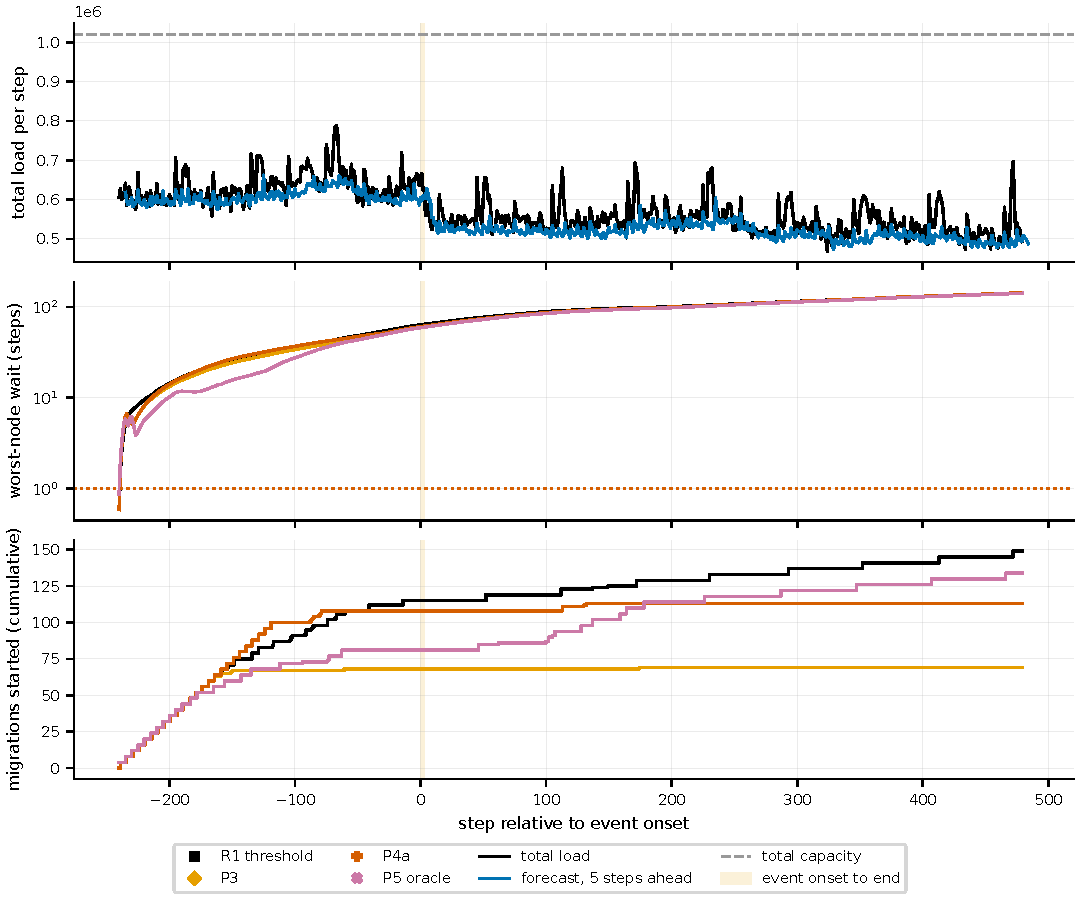
\includegraphics[width=\linewidth]{assets/figures/fa2_episode_D1.pdf}
\caption{FA2 and review Figure 3. Regenerated flash-crowd episode on D1: event D1-5320 (peak 1044), replicate 23. One replicate selected by a rule fixed beforehand, not an average, no interval. Rule: among the 30 sampled abrupt evaluation events of the default cell (m 5, headroom 1.6) the event with the median peak (lower middle on an even count, ties by event id), with the replicate index it has in the frozen rows. Top: total offered load per step, total node capacity and the point forecast of the P4 forecaster (lightgbm), summed over partitions, for the horizon of 5 steps (the default migration duration), the forecast made at step i drawn at its target step i + 5; P3 and P4a act on forecasts of this forecaster and P4a adds an interval margin that is not drawn; the shaded span runs from event onset to end. Middle: worst-node wait proxy in steps (symlog axis, SLO threshold 1 dotted). Bottom: migrations started, cumulative. Policies R1 (P1), P3 (forecaster of P4), P4a, P5. The regenerated damage and number of moves of every drawn policy equal the frozen rows (damage: R1 threshold 12.4552; P3 18.129; P4a 14.3718; P5 oracle 11.8953). Window 720 steps of 60 s, master\_seed 42. Sources: results\_frozen Must rows (P1, P3, P5) and Q1 AA6 rows (P4a), regenerated with the frozen code and configs; table of the comparison: figures/fa2\_episode\_check.csv.}\label{fig:fa2_episode_d1}
\end{figure}

% generated by build_assets.py from the recorded PDF and caption; do not edit
\begin{figure}[tbp]
\centering
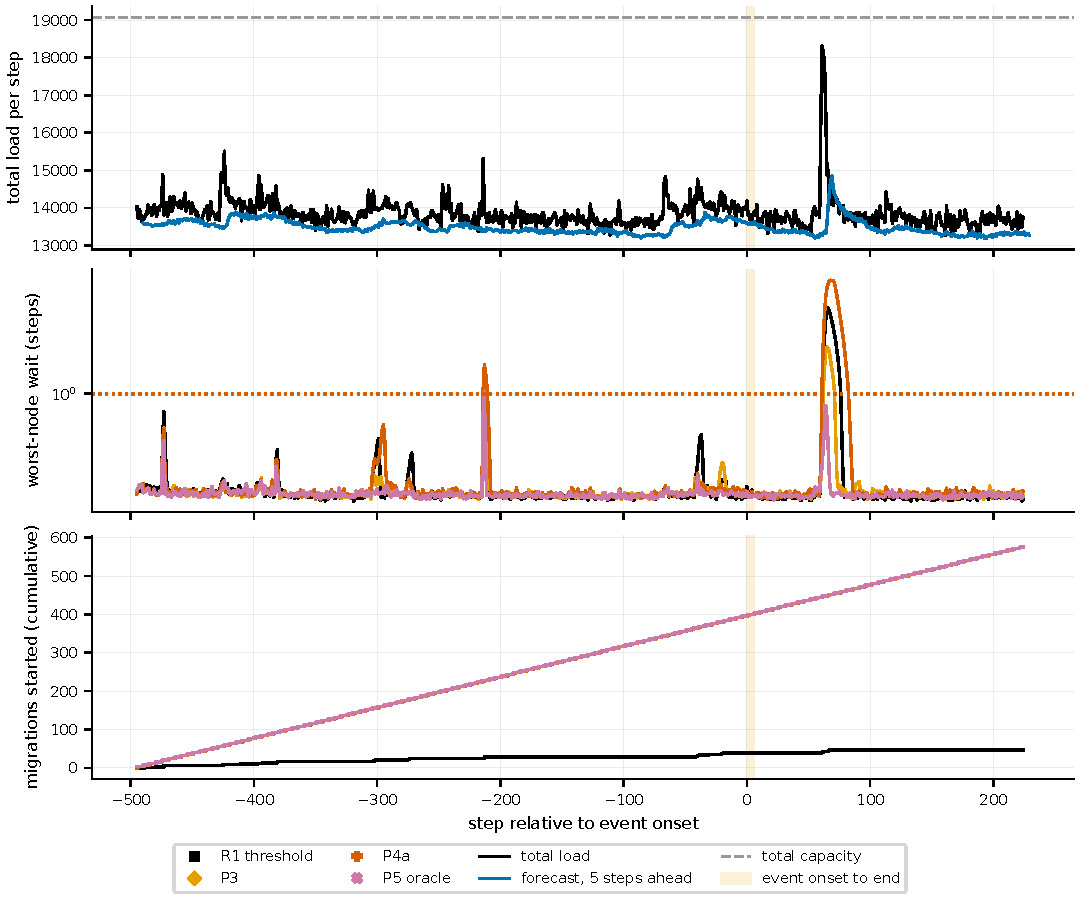
\includegraphics[width=\linewidth]{assets/figures/fa2_episode_D2.pdf}
\caption{FA2 and review Figure 3. Regenerated flash-crowd episode on D2: event D2-122 (peak 175), replicate 22. One replicate selected by a rule fixed beforehand, not an average, no interval. Rule: among the 30 sampled abrupt evaluation events of the default cell (m 5, headroom 1.6) the event with the median peak (lower middle on an even count, ties by event id), with the replicate index it has in the frozen rows. Top: total offered load per step, total node capacity and the point forecast of the P4 forecaster (lightgbm), summed over partitions, for the horizon of 5 steps (the default migration duration), the forecast made at step i drawn at its target step i + 5; P3 and P4a act on forecasts of this forecaster and P4a adds an interval margin that is not drawn; the shaded span runs from event onset to end. Middle: worst-node wait proxy in steps (symlog axis, SLO threshold 1 dotted). Bottom: migrations started, cumulative. Policies R1 (P1), P3 (forecaster of P4), P4a, P5. The regenerated damage and number of moves of every drawn policy equal the frozen rows (damage: R1 threshold 0.00330456; P3 0.00102777; P4a 0.00609227; P5 oracle 2.76524e-06). Window 720 steps of 10 s, master\_seed 42. Sources: results\_frozen Must rows (P1, P3, P5) and Q1 AA6 rows (P4a), regenerated with the frozen code and configs; table of the comparison: figures/fa2\_episode\_check.csv.}\label{fig:fa2_episode_d2}
\end{figure}

% generated by build_assets.py from the recorded PDF and caption; do not edit
\begin{figure}[tbp]
\centering
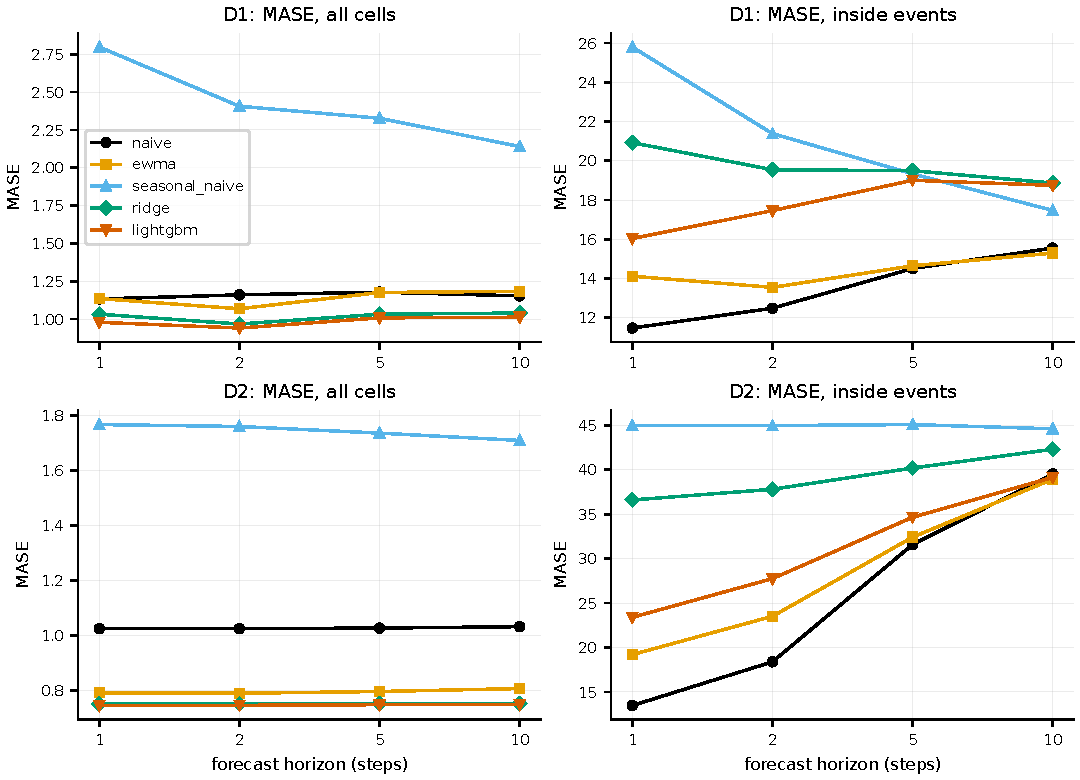
\includegraphics[width=\linewidth]{assets/figures/fa3_forecast_accuracy.pdf}
\caption{FA3. Forecast accuracy on the evaluation split, MASE over all cells and inside events, by forecaster and horizon, per dataset (D1, D2). Values are pooled point estimates from tables/forecast\_accuracy.csv; no interval is drawn because the table holds none. MASE is scaled by the training-prefix naive error, so 1 equals that scale. Source rows are rolling-refit forecasts; the stride-4 Chronos subset is not drawn (see tables/forecast\_accuracy\_chronos.csv). Seed: forecasts are deterministic given the stored tables (master seed 42).}\label{fig:fa3_forecast_accuracy}
\end{figure}

% generated by build_assets.py from the recorded PDF and caption; do not edit
\begin{figure}[tbp]
\centering
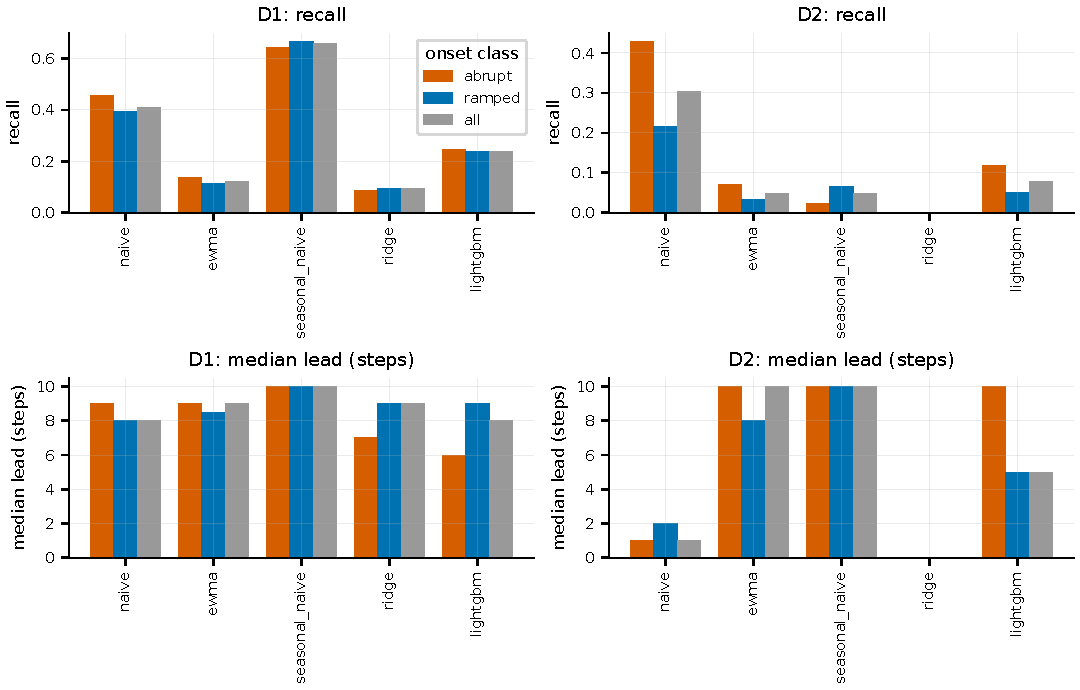
\includegraphics[width=\linewidth]{assets/figures/fa4_early_warning.pdf}
\caption{FA4. Early warning on the evaluation split: recall and median lead time (steps) of each forecaster by onset class, per dataset. Pooled point values from tables/forecast\_accuracy\_early\_warning.csv, no interval in the table. Events per class (naive row, after exclusions; other forecasters differ by the excluded events listed in the table): D1 all 3679; D1 abrupt 957; D1 ramped 2722; D2 all 102; D2 abrupt 42; D2 ramped 60. A missing bar means the value is undefined (no alarm raised). Precision is in the table and is not drawn.}\label{fig:fa4_early_warning}
\end{figure}

% generated by build_assets.py from the recorded PDF and caption; do not edit
\begin{figure}[tbp]
\centering
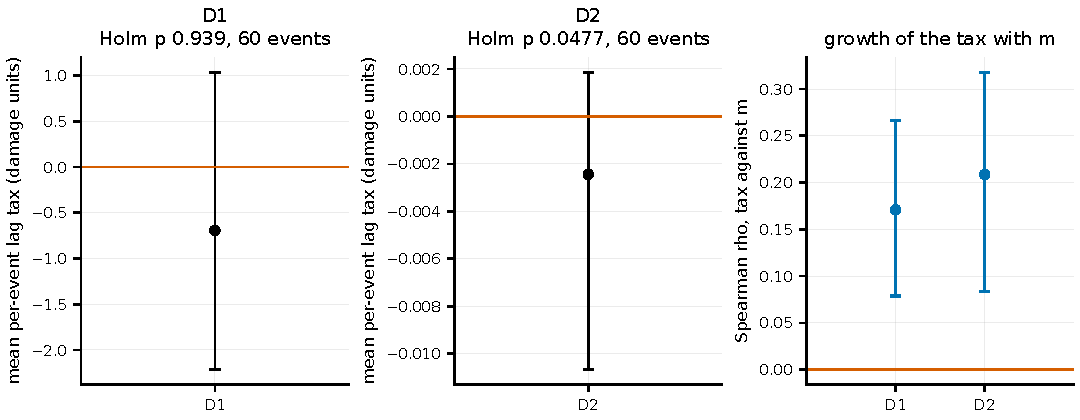
\includegraphics[width=\linewidth]{assets/figures/fa5_lag_tax.pdf}
\caption{FA5. Lag tax (reactive minus oracle damage) per event at the default m and headroom: mean with its 95\% BCa interval over events (9999 resamples, master seed 42) (left, per dataset, own axis because D1 and D2 damage scales differ), and Spearman rho of tax against m (right). Zero line marks no tax. 60 events per dataset; labels and Holm-adjusted p values are those of tables/c1\_lag\_tax.csv (family F1, 4 p values). Hypothesis labels are in the ledger.}\label{fig:fa5_lag_tax}
\end{figure}

% generated by build_assets.py from the recorded PDF and caption; do not edit
\begin{figure}[tbp]
\centering
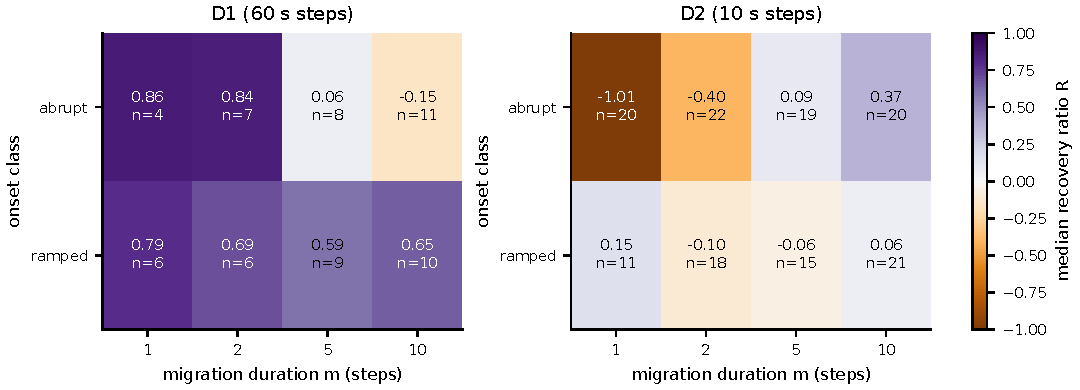
\includegraphics[width=\linewidth]{assets/figures/fa6_regime_must.pdf}
\caption{FA6b. Headline regime map on the real traces: median recovery ratio R of P3\_lightgbm by migration duration m and onset class at headroom 1.6, per dataset. Cell text is the median R over events with R defined and the number n of those events; blank cells have no event with R defined. Colour clipped to -1 to 1. Intervals and the share of replicates with R defined are in tables/regime\_map\_must.csv. Datasets are not pooled.}\label{fig:fa6_regime_must}
\end{figure}

% generated by build_assets.py from the recorded PDF and caption; do not edit
\begin{figure}[tbp]
\centering
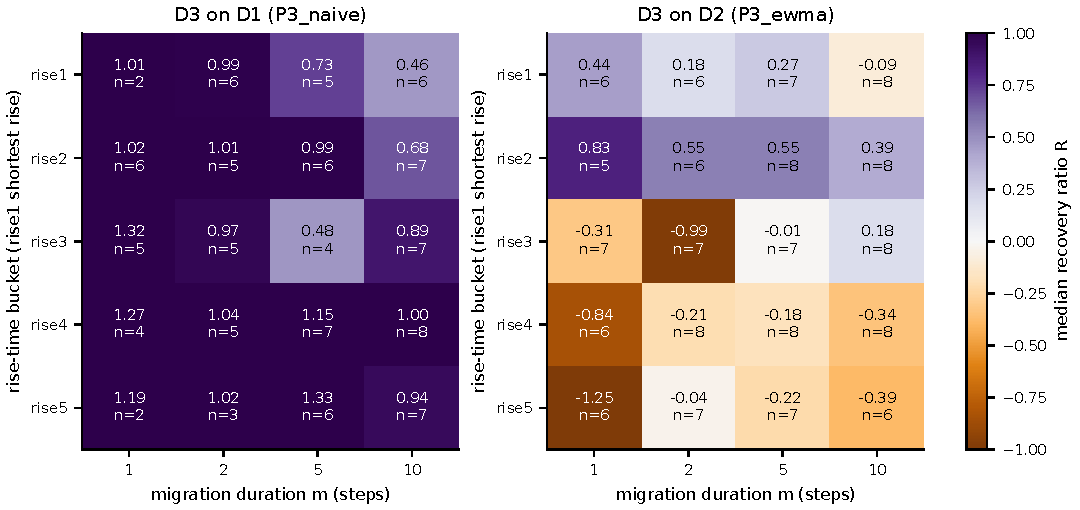
\includegraphics[width=\linewidth]{assets/figures/fa6_regime_q2.pdf}
\caption{FA6a. Measured lag-tax recovery ratio R across migration duration m (x) and flash-crowd rise-time bucket (y), headroom 1.6, injected-event data D3 on D1 and on D2 (forecast policy: P3\_ewma/P3\_naive). Cell text is the median R over events with R defined and the number n of those events (of 8 events per bucket); blank cells have no event with R defined. Colour is clipped to the range -1 to 1, the printed value is not clipped. R is defined only where the lag tax is at least the registered share of the reactive damage. Every cell rests on few events (flag in tables/regime\_map\_q2.csv); intervals are in the table. Datasets are not pooled.}\label{fig:fa6_regime_q2}
\end{figure}

% generated by build_assets.py from the recorded PDF and caption; do not edit
\begin{figure}[tbp]
\centering
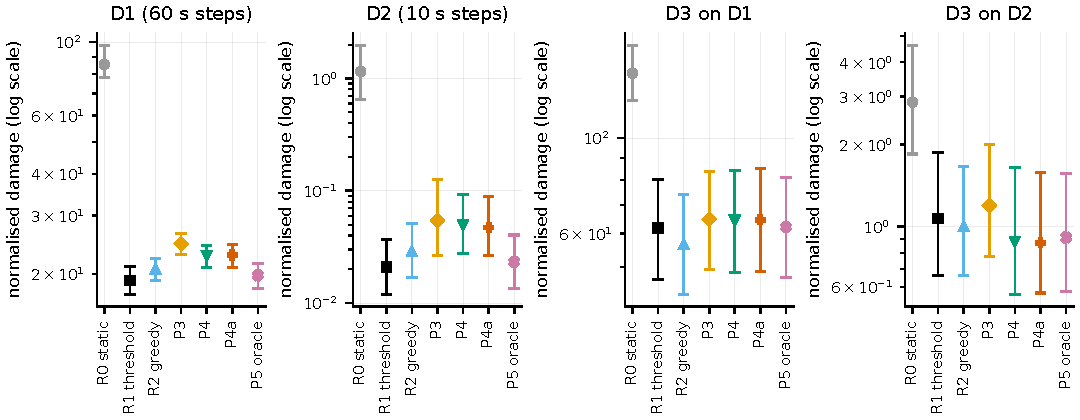
\includegraphics[width=\linewidth]{assets/figures/fa7_damage.pdf}
\caption{FA7a. Overall performance of the seven placement policies: mean per-event normalised damage with its 95\% BCa interval over events (9999 resamples, master seed 42), per dataset (log y axis, each panel its own scale; datasets are not pooled because D1 damage is about 20 and D2 about 0.02). R0, R1 and R2 are P0, P1 and P2. Events per dataset: D1 60; D2 60; D1\_D3 40; D2\_D3 40. Default m and headroom, 30 replicates per event, tables/rt\_policy\_metrics.csv (descriptive, not pre-registered).}\label{fig:fa7_damage}
\end{figure}

% generated by build_assets.py from the recorded PDF and caption; do not edit
\begin{figure}[tbp]
\centering
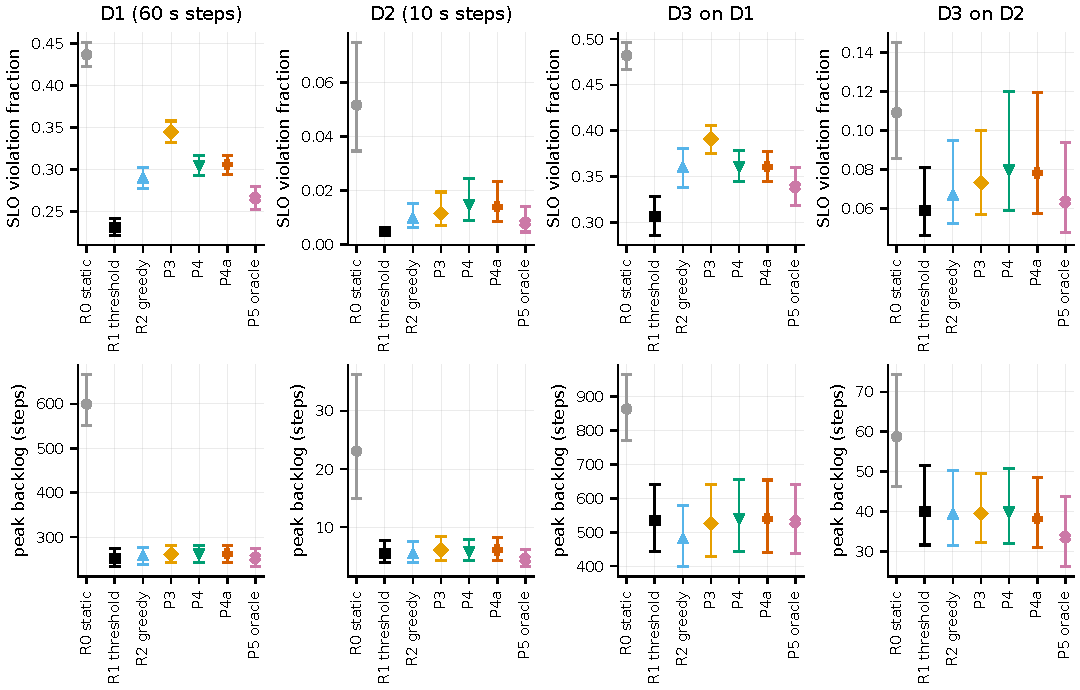
\includegraphics[width=\linewidth]{assets/figures/fa7_violation_backlog.pdf}
\caption{FA7b. SLO violation fraction (top) and peak backlog in steps (bottom) for the seven policies, per dataset: mean per-event value with its 95\% BCa interval over events (9999 resamples, master seed 42). R0, R1, R2 are P0, P1, P2. Events per dataset: D1 60; D2 60; D1\_D3 40; D2\_D3 40. Default m and headroom; tables/rt\_policy\_metrics.csv (descriptive, not pre-registered).}\label{fig:fa7_violation_backlog}
\end{figure}

% generated by build_assets.py from the recorded PDF and caption; do not edit
\begin{figure}[tbp]
\centering
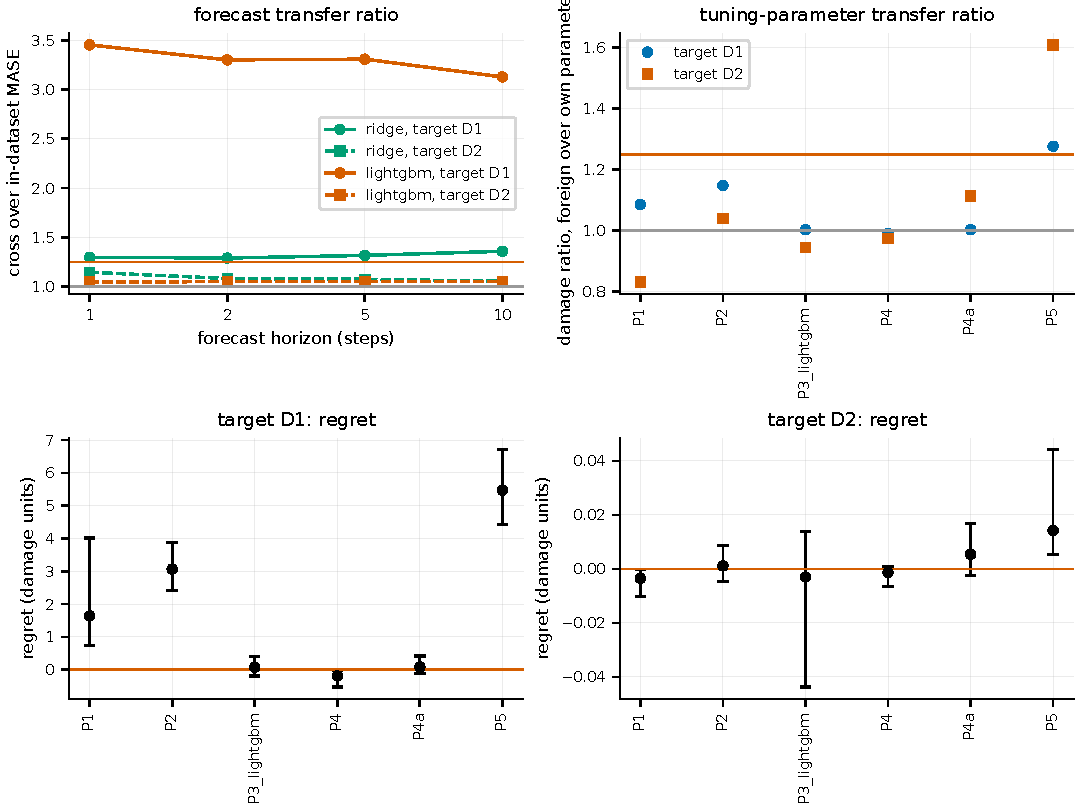
\includegraphics[width=\linewidth]{assets/figures/fa8_transfer.pdf}
\caption{FA8. Cross-dataset transfer. Top left: forecast transfer ratio (fixed model fitted on the source training prefix, scored on the target, over the same protocol in-dataset), ridge and lightgbm, by horizon and target. Top right: tuning-parameter transfer ratio of mean per-event damage, foreign over own parameters, per policy and target. Lines: 1 (grey) and the registered threshold 1.25 (orange). Bottom: regret (foreign minus own mean damage) with 95\% BCa interval over events (9999 resamples, master seed 42), per target on its own damage scale. Source: tables/c5\_transfer\_detail.csv; ratios have no interval in the table.}\label{fig:fa8_transfer}
\end{figure}

% generated by build_assets.py from the recorded PDF and caption; do not edit
\begin{figure}[tbp]
\centering
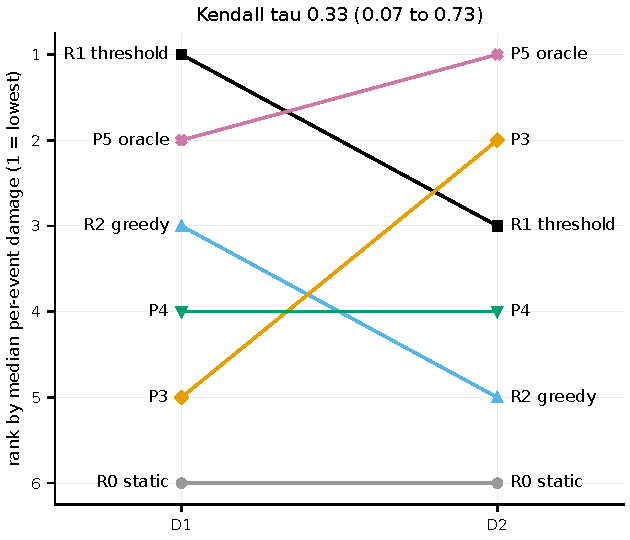
\includegraphics[width=\linewidth]{assets/figures/fa9_ranking.pdf}
\caption{FA9. Policy ranking on D1 and D2 by median per-event damage (60 events on D1, 60 on D2), rank 1 is the lowest damage. R0, R1, R2 are P0, P1, P2. Kendall tau between the two rankings, tau and its percentile bootstrap interval are in the title (6 policies, threshold 0.6 in tables/c6\_ranking\_tau.csv). Source: tables/c6\_ranking.csv.}\label{fig:fa9_ranking}
\end{figure}

% generated by build_assets.py from the recorded PDF and caption; do not edit
\begin{figure}[tbp]
\centering
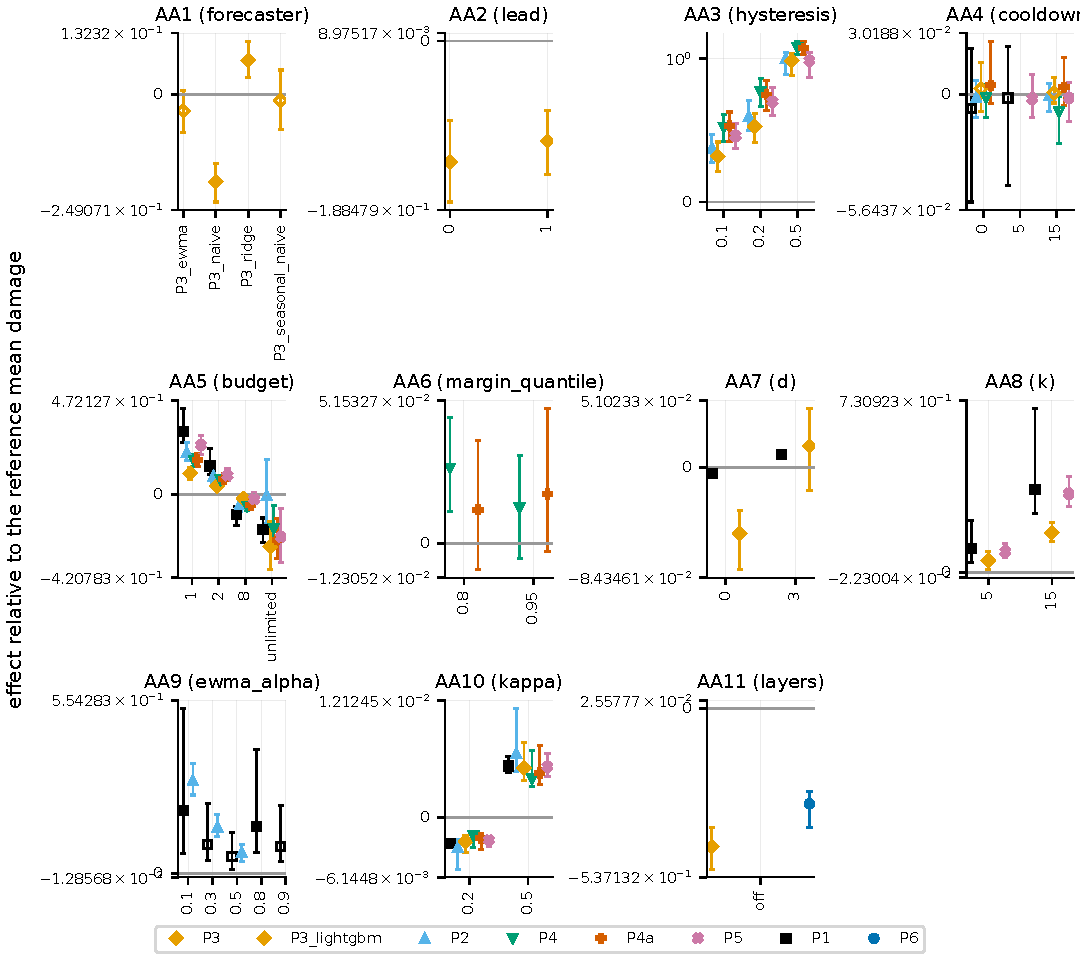
\includegraphics[width=\linewidth]{assets/figures/fa10_ablations_D1.pdf}
\caption{FA10 (D1). Ablation effects on mean per-event damage, level minus reference, as a multiple of the reference mean (symlog axis; 0 means no change, 1 means +100 percent), per ablation AA1 to AA11 and policy, with 95\% BCa interval over events (9999 resamples, master seed 42) over 60 events scaled by the reference mean. Filled markers: Holm-adjusted p below the registered alpha within the ablation; open markers: not. One factor at a time, levels not re-tuned; interactions untested; AA13, XA6 and FA16 were not completed. Source: tables/aa\_ablations.csv (descriptive, no hypothesis label).}\label{fig:fa10_ablations_d1}
\end{figure}

% generated by build_assets.py from the recorded PDF and caption; do not edit
\begin{figure}[tbp]
\centering
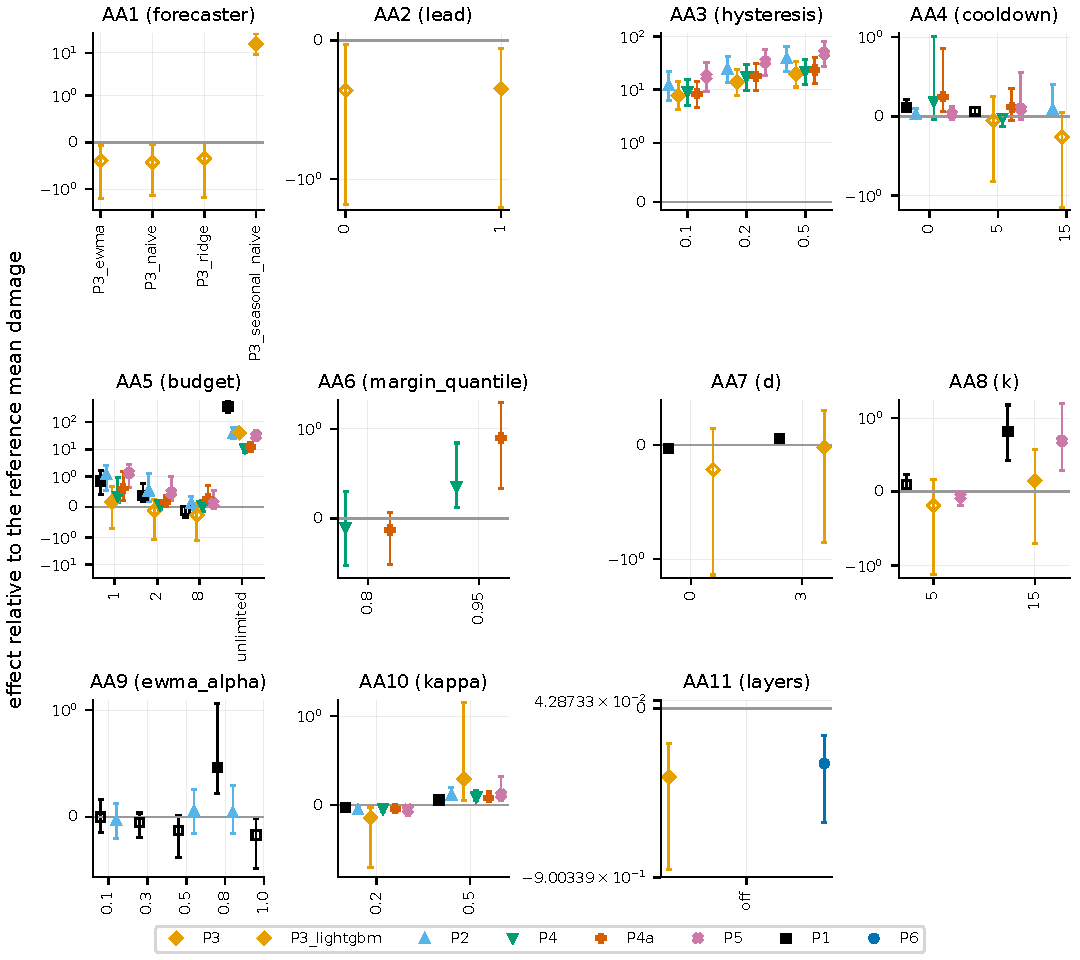
\includegraphics[width=\linewidth]{assets/figures/fa10_ablations_D2.pdf}
\caption{FA10 (D2). Ablation effects on mean per-event damage, level minus reference, as a multiple of the reference mean (symlog axis; 0 means no change, 1 means +100 percent), per ablation AA1 to AA11 and policy, with 95\% BCa interval over events (9999 resamples, master seed 42) over 60 events scaled by the reference mean. Filled markers: Holm-adjusted p below the registered alpha within the ablation; open markers: not. One factor at a time, levels not re-tuned; interactions untested; AA13, XA6 and FA16 were not completed. Source: tables/aa\_ablations.csv (descriptive, no hypothesis label).}\label{fig:fa10_ablations_d2}
\end{figure}

% generated by build_assets.py from the recorded PDF and caption; do not edit
\begin{figure}[tbp]
\centering
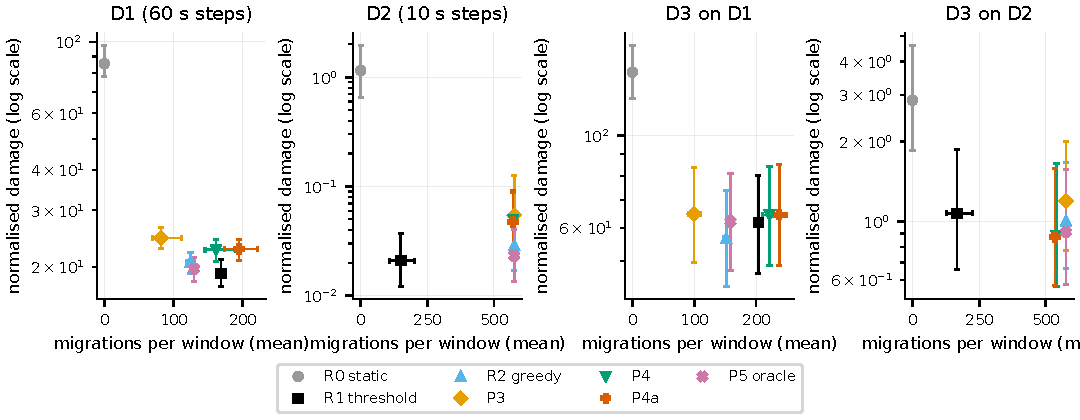
\includegraphics[width=\linewidth]{assets/figures/fa11_damage_moves.pdf}
\caption{FA11. Damage against migration count per policy, per dataset (each panel its own damage scale): mean per-event value with its 95\% BCa interval over events (9999 resamples, master seed 42) on both axes. R0, R1, R2 are P0, P1, P2; R0 never migrates. Events per dataset: D1 60; D2 60; D1\_D3 40; D2\_D3 40. Default m and headroom; tables/rt\_policy\_metrics.csv (descriptive, not pre-registered).}\label{fig:fa11_damage_moves}
\end{figure}

% generated by build_assets.py from the recorded PDF and caption; do not edit
\begin{figure}[tbp]
\centering
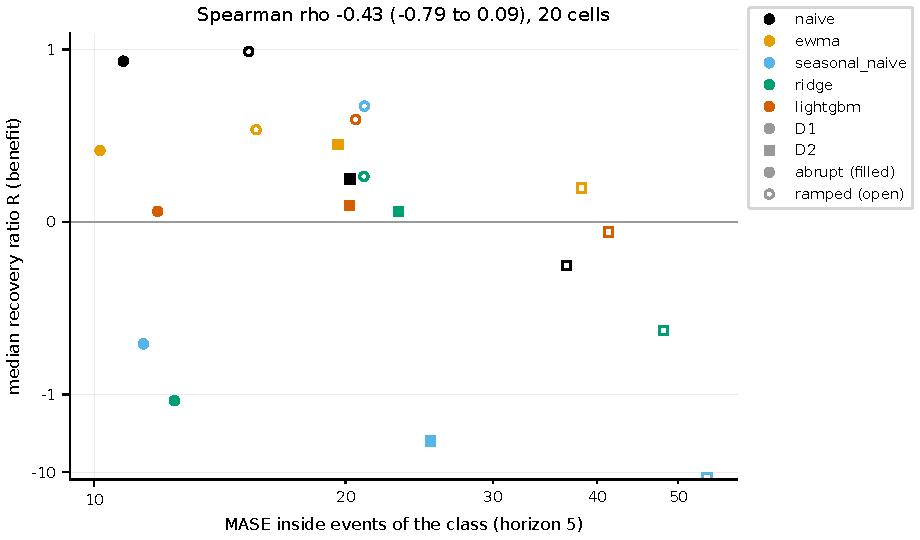
\includegraphics[width=\linewidth]{assets/figures/fa12_mase_benefit.pdf}
\caption{FA12. Forecast accuracy against control benefit: one point per cell (forecaster, dataset, onset class), x is the MASE inside events of that class at the horizon nearest m plus d, y is the cell median recovery ratio R. Circles: D1, squares: D2; filled: abrupt, open: ramped. Spearman rho with its 95\% BCa interval over events (9999 resamples, master seed 42) over cells is in the title (exploratory p 0.0594); cell benefits rest on the events with R defined (8 to 19 per cell, tables/c4\_accuracy\_benefit\_cells.csv). Symlog y axis.}\label{fig:fa12_mase_benefit}
\end{figure}

% generated by build_assets.py from the recorded PDF and caption; do not edit
\begin{figure}[tbp]
\centering
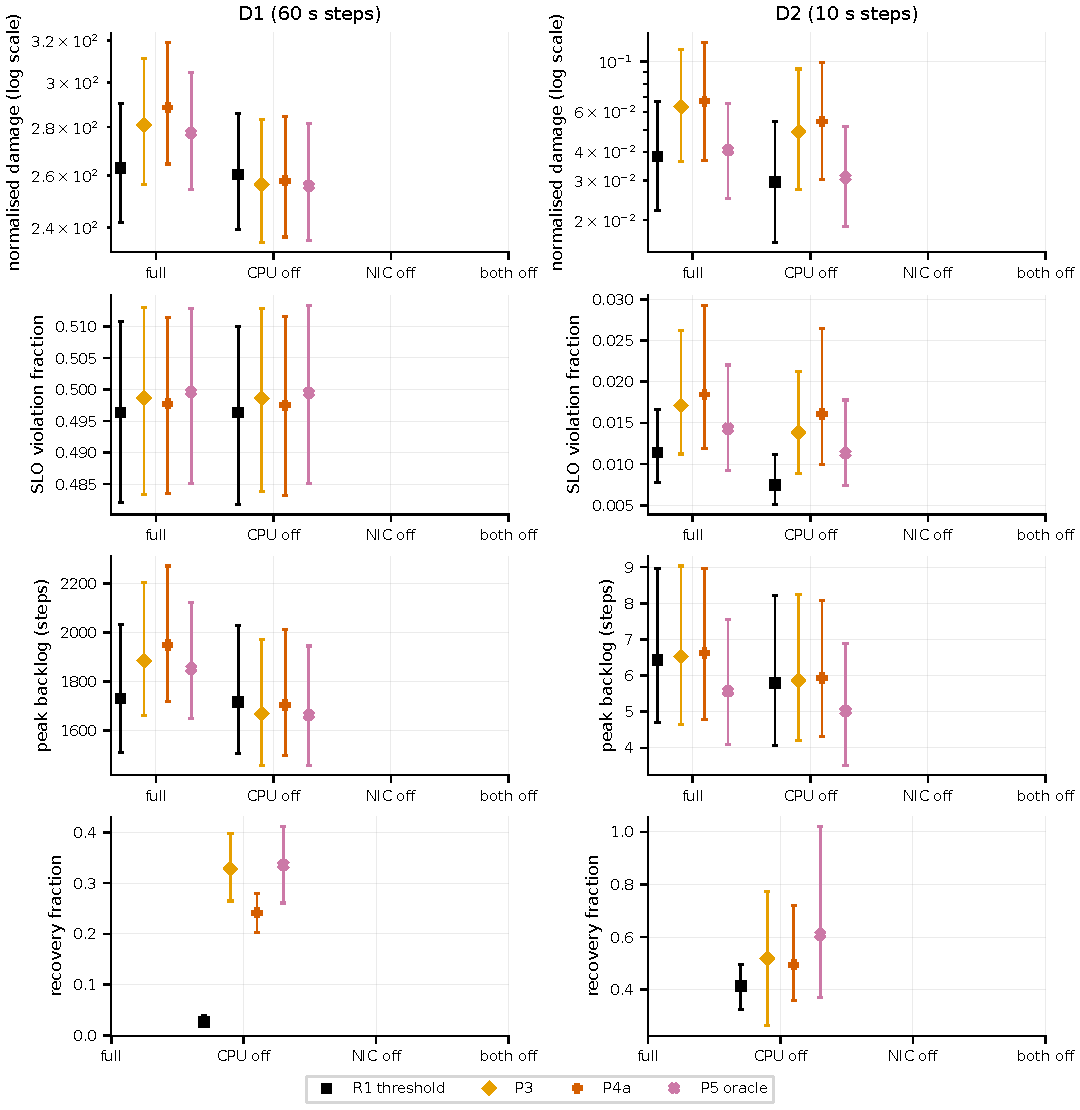
\includegraphics[width=\linewidth]{assets/figures/fa13_contention.pdf}
\caption{FA13. Contention ablation (RV1) in the coupled model, per dataset (each panel its own scale): mean per-event damage (log scale), SLO violation fraction and peak backlog with their 95\% BCa interval over events (9999 resamples, master seed 42), and the recovery fraction of tables/rv1\_contention.csv (bottom row; blank where it is undefined, which includes the full model, the reference). Levels: full model, CPU contention off, NIC contention off, both off. The constant-m control mode is in the tables and not drawn. Events per dataset: D1 60; D2 60. Tables: tables/rt\_rv1\_metrics.csv (descriptive, not pre-registered) and tables/rv1\_contention.csv.}\label{fig:fa13_contention}
\end{figure}

% generated by build_assets.py from the recorded PDF and caption; do not edit
\begin{figure}[tbp]
\centering
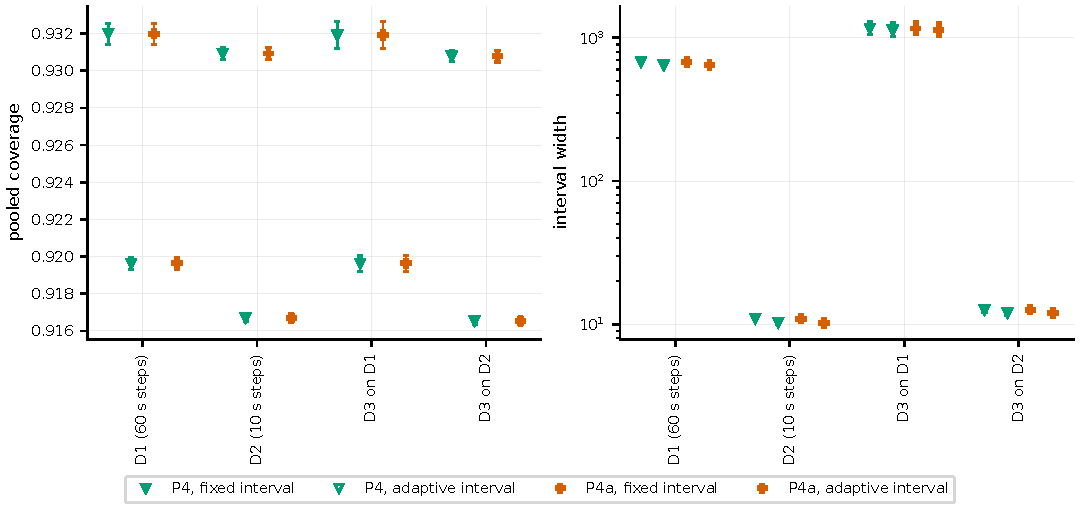
\includegraphics[width=\linewidth]{assets/figures/fa14_conformal_logging.pdf}
\caption{FA14. Conformal interval logging (RV4): pooled coverage (left) and interval width (right, log scale) of the fixed and the adaptive interval, for P4 and P4a, per dataset (widths are not comparable across datasets). Filled markers: fixed interval; open: adaptive. Mean with its 95\% BCa interval over events (9999 resamples, master seed 42). The table holds pooled values, so there is no time axis; the adaptive level (alpha), the point error and the trigger counts are in the table and not drawn. Events per dataset: D1 60; D2 60; D1\_D3 40; D2\_D3 40. Source: tables/rv4\_logging.csv.}\label{fig:fa14_conformal_logging}
\end{figure}

% generated by build_assets.py from the recorded PDF and caption; do not edit
\begin{figure}[tbp]
\centering
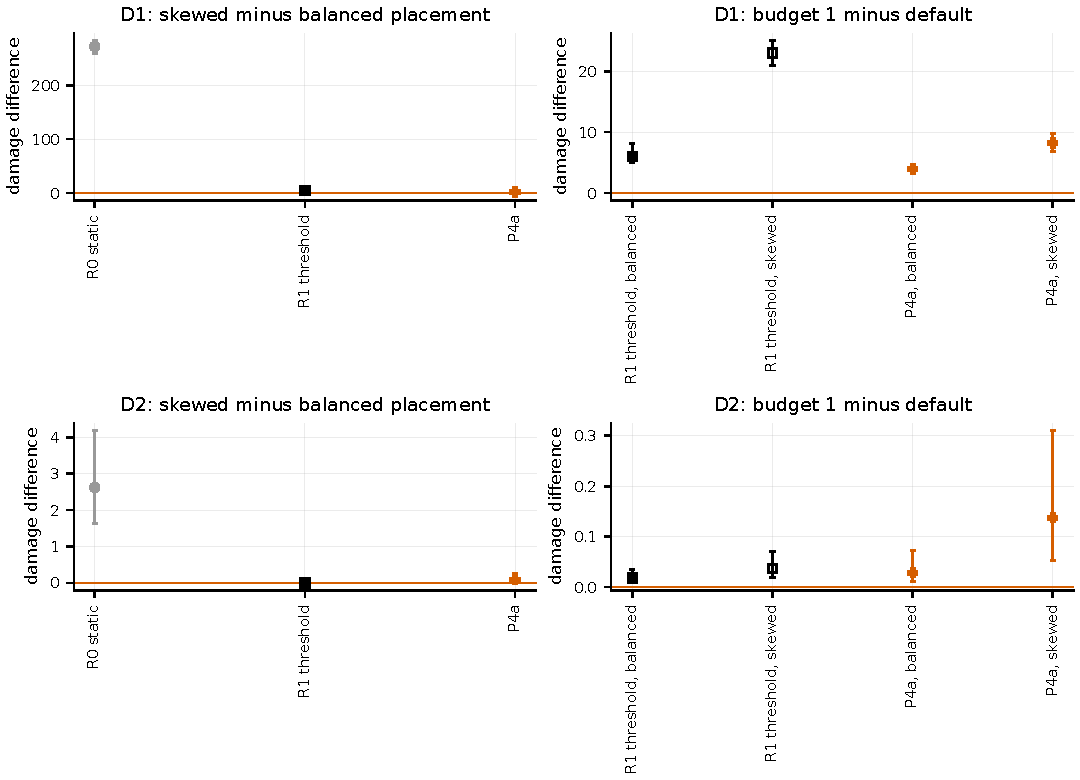
\includegraphics[width=\linewidth]{assets/figures/fa15_placement_budget.pdf}
\caption{FA15. Placement and migration budget (RV2, RV3), per dataset (each panel its own damage scale). Left: mean per-event damage under skewed placement minus balanced placement, for R0, R1 and P4a. Right: mean per-event damage with migration budget 1 minus the default budget, for R1 and P4a, under balanced placement (filled) and skewed placement (open). Mean difference with its 95\% BCa interval over events (9999 resamples, master seed 42); zero line marks no difference. R0, R1 are P0, P1. Events per dataset: D1 60; D2 60. Sources: tables/rv2\_placement.csv and tables/rv3\_budget.csv. Review figure 10 asked for the throttled policy; the recorded RV3 rows hold the budget-1 contrast, which is what is drawn.}\label{fig:fa15_placement_budget}
\end{figure}

 once
% needs: booktabs, longtable, adjustbox, graphicx
% generated by build_assets.py from the recorded CSV; do not edit
\begin{table}[tbp]
\centering
\scriptsize
\caption{Datasets}\label{tab:ta1}
\adjustbox{max width=\linewidth}{%
\begin{tabular}{llrrrrrrrrrrrl}
\toprule
dataset & role & step seconds & n steps & span days & n partitions & train end & tune end & eval steps & n events & events eval abrupt & events eval ramped & events eval all & bytes provenance \\
\midrule
D1 & primary real trace & 60 & 10080 & 7 & 512 & 2880 & 4320 & 5760 & 6482 & 964 & 2743 & 0 & assumed \\
D2 & second real trace & 10 & 18508 & 2.142 & 512 & 4627 & 7403 & 11105 & 177 & 42 & 60 & 0 & real \\
D1\_D3 & D1 with injected events & 60 & 10080 & 7 & 512 & 2880 & 4320 & 5760 & 40 & 0 & 0 & 40 & assumed \\
D2\_D3 & D2 with injected events & 10 & 18508 & 2.142 & 512 & 4627 & 7403 & 11105 & 40 & 0 & 0 & 40 & real \\
\bottomrule
\end{tabular}}
\end{table}

% generated by build_assets.py from the recorded CSV; do not edit
{\scriptsize
\setlength{\tabcolsep}{3pt}
\begin{longtable}{lllll}
\caption{Parameters with real, assumed or design tag}\label{tab:ta2}\\
\toprule
key & parent & value & real or assumed & justification \\
\midrule
\endfirsthead
\toprule
key & parent & value & real or assumed & justification \\
\midrule
\endhead
\bottomrule
\endfoot
enabled & layers & false & design & n/a \\
n\_partitions & n/a & 512 & real & n/a \\
n\_nodes & n/a & 16 & real & n/a \\
headroom & n/a & 1.6 & assumed & n/a \\
slo\_threshold & n/a & 1 & design & n/a \\
window\_steps & n/a & 720 & design & n/a \\
step\_seconds & n/a & 60 & real & n/a \\
migration\_steps\_m0 & n/a & 5 & assumed & n/a \\
migration\_overhead\_kappa & n/a & 0.3 & assumed & n/a \\
migration\_budget\_B & n/a & 4 & design & n/a \\
monitor\_delay\_d & n/a & 1 & design & n/a \\
decision\_interval\_k & n/a & 1 & design & n/a \\
horizons & n/a & [1, 2, 5, 10] & design & n/a \\
refit\_interval & n/a & 360 & assumed & n/a \\
seasonal\_period & n/a & 1440 & real & n/a \\
tuning\_budget & n/a & 36 & design & n/a \\
tune\_plateau\_tol & n/a & 0.05 & assumed & n/a \\
ewma\_alpha\_grid & n/a & [0.1, 0.3, 0.5, 0.8] & design & n/a \\
theta\_hi\_grid & n/a & [0.8, 0.9, 1.0] & design & n/a \\
cooldown\_grid & n/a & [0, 5, 15] & design & n/a \\
hysteresis\_grid & n/a & [0.0, 0.1, 0.2, 0.5] & design & n/a \\
oracle\_window\_grid & n/a & [1, 5, 10] & design & n/a \\
margin\_quantile & n/a & 0.9 & design & n/a \\
replicates\_per\_cell & n/a & 30 & design & n/a \\
min\_replicates & n/a & 30 & design & n/a \\
m\_levels & n/a & [1, 2, 5, 10] & design & n/a \\
headroom\_levels & n/a & [1.3, 1.6, 2.0] & design & n/a \\
pilot\_replicates & n/a & 5 & design & n/a \\
oracle\_check\_events & n/a & 100 & design & n/a \\
n\_boot & n/a & 9999 & design & n/a \\
ci\_level & n/a & 0.95 & design & n/a \\
r & n/a & 5 & design & n/a \\
W\_b & n/a & 60 & design & n/a \\
s & n/a & 3 & design & n/a \\
eps & n/a & 0.001 & design & n/a \\
rise\_lo & n/a & 0.1 & design & n/a \\
rise\_hi & n/a & 0.9 & design & n/a \\
simplex\_step & n/a & 0.1 & design & n/a \\
min\_events & n/a & 24 & design & n/a \\
min\_lag\_tax\_share & n/a & 0.05 & design & n/a \\
capacity\_jitter\_frac & n/a & 0.1 & assumed & n/a \\
wasted\_move\_window & n/a & 10 & design & n/a \\
inject\_tolerance & n/a & 5 & design & n/a \\
injection\_amplitude\_min & n/a & 10 & assumed & n/a \\
injection\_amplitude\_max & n/a & 100 & assumed & n/a \\
injection\_rise\_min & n/a & 2 & assumed & n/a \\
injection\_rise\_max & n/a & 10 & assumed & n/a \\
injection\_dur\_min & n/a & 10 & assumed & n/a \\
injection\_dur\_max & n/a & 50 & assumed & n/a \\
cpu\_cores & n/a & 8 & real & n/a \\
h\_net & n/a & 2 & assumed & n/a \\
rho & n/a & 0.25 & assumed & n/a \\
sigma\_size & n/a & 0.5 & assumed & n/a \\
phi & n/a & 1 & assumed & n/a \\
master\_seed & n/a & 42 & design & n/a \\
hash\_seed & n/a & 'seed1' & design & n/a \\
reserved\_cores & n/a & 1 & design & n/a \\
workers & n/a & 7 & design & n/a \\
compute\_budget\_core\_hours & n/a & 288 & real & n/a \\
runner\_stall\_minutes & n/a & 30 & design & n/a \\
cleanroom\_stride & n/a & 1 & design & n/a \\
d2\_max\_gb & n/a & 2 & real & n/a \\
azure\_days & n/a & 7 & real & n/a \\
azure\_skip\_cols & n/a & 4 & real & n/a \\
d2\_min\_cols & n/a & 4 & real & n/a \\
c0 & n/a & 1 & assumed & n/a \\
c1 & n/a & 0 & assumed & n/a \\
azure\_mins\_per\_day & n/a & 1440 & real & n/a \\
data\_root & n/a & 'data' & real & n/a \\
ridge\_alpha & n/a & [0.1, 1.0, 10.0] & design & n/a \\
lightgbm\_leaves & n/a & [15, 31, 63] & design & n/a \\
gamma & n/a & 0.005 & design & ACI step size, the value used in the A15 experiments (Gibbs and Candes 2021, Sec 2.1), not tuned here (A26) \\
a\_min & n/a & 0.01 & assumed & n/a \\
a\_max & n/a & 0.2 & assumed & n/a \\
residual\_window & n/a & 100 & design & n/a \\
psi\_grid & n/a & [0.1, 0.2, 0.5] & design & n/a \\
io\_chunk\_bytes & compute & 65536 & design & n/a \\
snapshots & paths & 'snapshots' & design & n/a \\
default\_tag & snapshot & 'prereg-v1' & design & n/a \\
tag\_pattern & snapshot & '[a-zA-Z0-9\_-]+' & design & n/a \\
sources & snapshot & ['src', 'scripts', 'configs'] & design & n/a \\
ignore\_patterns & snapshot & ['*.pyc', '\_\_pycache\_\_'] & design & n/a \\
manifest\_name & snapshot & 'manifest.json' & design & n/a \\
raw\_dirname & n/a & 'raw' & design & n/a \\
azure\_dirname & n/a & 'azure2019' & design & n/a \\
twitter\_dirname & n/a & 'twitter' & design & n/a \\
processed\_dirname & n/a & 'processed' & design & n/a \\
logs\_dirname & n/a & 'logs' & design & n/a \\
amendments\_file & n/a & 'AMENDMENTS.md' & design & n/a \\
d2\_file & n/a & 'cluster53.sort.zst' & real & n/a \\
azure\_invocation\_pattern & n/a & 'invocations\_per\_function\_md.anon.d\{day:02d\}.csv' & real & n/a \\
azure\_duration\_pattern & n/a & 'function\_durations\_percentiles.anon.d\{day:02d\}.csv' & real & n/a \\
azure\_memory\_pattern & n/a & 'app\_memory\_percentiles.anon.d\{day:02d\}.csv' & real & n/a \\
azure\_head\_cols & n/a & ['HashOwner', 'HashApp', 'HashFunction', 'Trigger'] & real & n/a \\
azure\_id\_cols & n/a & ['HashOwner', 'HashApp', 'HashFunction'] & real & n/a \\
azure\_dur\_avg\_col & n/a & 'Average' & real & n/a \\
azure\_dur\_count\_col & n/a & 'Count' & real & n/a \\
azure\_memory\_cols & n/a & ['HashOwner', 'HashApp', 'SampleCount', 'AverageAllocatedMb', 'AverageAllocatedMb\_pct1', 'AverageAllocatedMb\_pct5', 'AverageAllocatedMb\_pct25', 'AverageAllocatedMb\_pct50', 'AverageAllocatedMb\_pct75', 'AverageAllocatedMb\_pct95', 'AverageAllocatedMb\_pct99', 'AverageAllocatedMb\_pct100'] & real & n/a \\
azure\_chunk\_rows & n/a & 5000 & design & n/a \\
d2\_chunk\_rows & n/a & 2000000 & design & n/a \\
d2\_cols & n/a & ['timestamp', 'key', 'key\_size', 'value\_size', 'client', 'op', 'ttl'] & real & n/a \\
d2\_time\_col & n/a & 'timestamp' & real & n/a \\
d2\_key\_col & n/a & 'key' & real & n/a \\
d2\_ksize\_col & n/a & 'key\_size' & real & n/a \\
d2\_vsize\_col & n/a & 'value\_size' & real & n/a \\
d2\_op\_col & n/a & 'op' & real & n/a \\
d2\_step\_seconds & n/a & 10 & design & n/a \\
d1\_train\_days & n/a & 2 & design & n/a \\
d1\_tune\_days & n/a & 1 & design & n/a \\
d2\_split\_fractions & n/a & [0.25, 0.15] & design & n/a \\
key\_sep & n/a & '|' & design & n/a \\
hash\_bits & n/a & 128 & real & n/a \\
d1\_bytes\_sigma & n/a & 0.5 & assumed & n/a \\
d1\_bytes\_label & n/a & 'bytes' & design & n/a \\
demand\_fallback & n/a & 1 & assumed & n/a \\
inject\_label & n/a & 'D3' & design & n/a \\
injection\_events & n/a & 40 & design & n/a \\
injection\_hot\_min & n/a & 1 & assumed & n/a \\
injection\_hot\_max & n/a & 4 & assumed & n/a \\
wait\_quantile & n/a & 0.99 & design & n/a \\
tune\_replicates & n/a & 35 & design & n/a \\
tune\_plateau\_frac & n/a & 0.25 & design & n/a \\
seed\_bits & n/a & 32 & design & n/a \\
day\_seconds & n/a & 86400 & real & n/a \\
lookback\_L & n/a & 30 & design & n/a \\
roll\_window & n/a & 10 & design & n/a \\
forecast\_ewma\_alpha & n/a & 0.3 & design & n/a \\
origin\_stride & n/a & 4 & design & n/a \\
lgbm\_trees & n/a & 100 & design & n/a \\
lgbm\_lr & n/a & 0.1 & design & n/a \\
lgbm\_verbosity & n/a & -1 & design & n/a \\
feature\_chunk\_origins & n/a & 256 & design & n/a \\
forecaster\_names & n/a & ['naive', 'ewma', 'seasonal\_naive', 'ridge', 'lightgbm'] & design & n/a \\
warn\_ratio & n/a & 3 & design & n/a \\
warn\_baseline\_window & n/a & 60 & design & n/a \\
smape\_eps & n/a & 0.001 & design & n/a \\
forecast\_dirname & n/a & 'forecasts' & design & n/a \\
h\_net\_levels & n/a & [1.3, 2.0, 4.0] & assumed & n/a \\
phi\_levels & n/a & [1.0, 0.1, 0.01] & assumed & n/a \\
size\_label & n/a & 'part\_size' & design & n/a \\
budget\_levels & n/a & [1, 2, 8, 'unlimited'] & design & AA5 levels besides the default 4; unlimited means n\_partitions (A34) \\
margin\_levels & n/a & [0.8, 0.9, 0.95] & design & AA6 margin levels for P4 and P4a (A34) \\
lead\_levels & n/a & [0, 1] & design & AA2 steps ahead of t the policy targets besides the default m: current step 0, next step 1 (A34) \\
rise\_buckets & n/a & 5 & design & D3 rise-time buckets of equal event count (A36) \\
D1 & q2\_forecast\_variants & P3\_naive & design & 14.9053 against P4 15.8977 and P3\_ewma 15.5024 \\
D2 & q2\_forecast\_variants & P3\_ewma & design & 0.00285714 against P3\_naive 0.00480893 and P4 0.0683602 \\
interaction\_effect\_frac & n/a & 0.05 & design & minimum effect size, as a fraction of the default mean damage, for a Q1 factor to count as active in the interaction trigger (A38) \\
interaction\_min\_active & n/a & 2 & design & the interaction trigger fires for a dataset and policy when at least this many factors are active (A38) \\
skew\_hot\_share & n/a & 0.25 & design & RV2 skewed placement: share of partitions, heaviest by training-prefix mean load, packed on the hot nodes (A38) \\
skew\_hot\_nodes & n/a & 4 & design & RV2 skewed placement: number of hot nodes, the first nodes in index order (A38) \\
kappa\_levels & n/a & [0.2, 0.3, 0.5] & assumed & AA10 migration overhead levels (guide section 3); the default 0.3 rows come from the Must grid and Q1 AA6 (A41) \\
d3\_learned\_forecasters & n/a & ['lightgbm'] & design & learned forecasters whose D3 tables are built for RV0, tuned hyperparameter of the source dataset (A42) \\
throttle\_budget\_B & n/a & 1 & design & RV3 throttled policy: the lowest AA5 budget level, against the default migration\_budget\_B (A45) \\
monitor\_delay\_levels & n/a & [0, 1, 3] & design & AA7 monitoring delay d, the guide config table; the default 1 is skipped in Q6 (A49) \\
decision\_interval\_levels & n/a & [1, 5, 15] & design & AA8 decision interval k, the guide config table; the default 1 is skipped in Q6 (A49) \\
chronos\_model & n/a & 'amazon/chronos-bolt-small' & design & n/a \\
chronos\_context & n/a & 128 & design & n/a \\
chronos\_stride & n/a & 4 & design & n/a \\
chronos\_quantile & n/a & 0.5 & design & n/a \\
chronos\_batch & n/a & 512 & design & n/a \\
h2\_split & n/a & 0.5 & design & H2 split on the median recovery ratio R between abrupt and ramped onsets (guide Section 3 config table; A56) \\
h3\_ub & n/a & 0.2 & design & H3 upper bound on median R at m = 1 (guide Section 3 config table; A56) \\
h4\_rho & n/a & 0.5 & design & H4 bound on the absolute Spearman correlation of MASE with placement benefit (guide Section 3 config table; A56) \\
h4\_ub & n/a & 0.7 & design & H4 bound on the upper end of the BCa interval of that correlation (guide Section 3 config table; A56) \\
h5\_ratio & n/a & 1.25 & design & H5 minimum transfer ratio, cross-dataset over in-dataset (guide Section 3 config table; A56) \\
h6\_tau & n/a & 0.6 & design & H6 minimum Kendall tau of the D1 and D2 policy rankings (guide Section 3 config table; A56) \\
h9\_share & n/a & 0.05 & design & H9 minimum share of violating node-steps attributed to the network or migration layer (guide Section 3 config table; A56) \\
alpha\_adj & n/a & 0.05 & design & significance level after Holm correction, every family (guide Section 3 config table; A56) \\
h12\_noninf & n/a & 0.02 & design & H12 non-inferiority margin for the damage of P4a against P4 (guide Section 3 config table; A56) \\
must & result\_folders & 'results' & design & n/a \\
q1 & result\_folders & 'results/q1' & design & n/a \\
q2 & result\_folders & 'results/q2' & design & n/a \\
q3 & result\_folders & 'results/q3' & design & n/a \\
q4 & result\_folders & 'results/q4' & design & n/a \\
q6 & result\_folders & 'results/q6' & design & n/a \\
q8 & result\_folders & 'results/q8' & design & n/a \\
q11\_rv0 & result\_folders & 'results/q11\_rv0' & design & n/a \\
q11\_rv123 & result\_folders & 'results/q11\_rv123' & design & n/a \\
\end{longtable}
}

% generated by build_assets.py from the recorded CSV; do not edit
{\scriptsize
\setlength{\tabcolsep}{3pt}
\begin{longtable}{lllrrrrrrrrlr}
\caption{Forecast accuracy}\label{tab:ta3}\\
\toprule
dataset & forecaster & split & horizon & mase all & smape all & mase event & smape event & n cells all & n cells event & n zero scale & origin subset & n origins \\
\midrule
\endfirsthead
\toprule
dataset & forecaster & split & horizon & mase all & smape all & mase event & smape event & n cells all & n cells event & n zero scale & origin subset & n origins \\
\midrule
\endhead
\bottomrule
\endfoot
D1 & ewma & eval & 1 & 1.136 & 0.2563 & 14.11 & 0.5669 & 2948608 & 25542 & 0 & all\_origins & n/a \\
D1 & ewma & eval & 2 & 1.068 & 0.268 & 13.55 & 0.7164 & 2948096 & 25526 & 0 & all\_origins & n/a \\
D1 & ewma & eval & 5 & 1.176 & 0.2696 & 14.65 & 0.9742 & 2946560 & 25473 & 0 & all\_origins & n/a \\
D1 & ewma & eval & 10 & 1.184 & 0.2783 & 15.29 & 1.102 & 2944000 & 25398 & 0 & all\_origins & n/a \\
D1 & lightgbm & eval & 1 & 0.9792 & 0.1925 & 16.04 & 0.6258 & 2948608 & 25542 & 0 & all\_origins & n/a \\
D1 & lightgbm & eval & 2 & 0.9411 & 0.2063 & 17.46 & 0.8711 & 2948096 & 25526 & 0 & all\_origins & n/a \\
D1 & lightgbm & eval & 5 & 1.008 & 0.2205 & 19.01 & 1.143 & 2946560 & 25473 & 0 & all\_origins & n/a \\
D1 & lightgbm & eval & 10 & 1.013 & 0.2317 & 18.75 & 1.33 & 2944000 & 25398 & 0 & all\_origins & n/a \\
D1 & naive & eval & 1 & 1.133 & 0.2573 & 11.47 & 0.4494 & 2948608 & 25542 & 0 & all\_origins & n/a \\
D1 & naive & eval & 2 & 1.16 & 0.2813 & 12.48 & 0.6477 & 2948096 & 25526 & 0 & all\_origins & n/a \\
D1 & naive & eval & 5 & 1.178 & 0.2615 & 14.51 & 1.016 & 2946560 & 25473 & 0 & all\_origins & n/a \\
D1 & naive & eval & 10 & 1.153 & 0.263 & 15.55 & 1.17 & 2944000 & 25398 & 0 & all\_origins & n/a \\
D1 & ridge & eval & 1 & 1.033 & 0.207 & 20.92 & 0.8495 & 2948608 & 25542 & 0 & all\_origins & n/a \\
D1 & ridge & eval & 2 & 0.9676 & 0.2196 & 19.54 & 1.062 & 2948096 & 25526 & 0 & all\_origins & n/a \\
D1 & ridge & eval & 5 & 1.033 & 0.2296 & 19.49 & 1.29 & 2946560 & 25473 & 0 & all\_origins & n/a \\
D1 & ridge & eval & 10 & 1.04 & 0.2405 & 18.87 & 1.421 & 2944000 & 25398 & 0 & all\_origins & n/a \\
D1 & seasonal\_naive & eval & 1 & 2.798 & 0.3526 & 25.8 & 0.9059 & 2948608 & 25542 & 0 & all\_origins & n/a \\
D1 & seasonal\_naive & eval & 2 & 2.407 & 0.3526 & 21.38 & 0.906 & 2948096 & 25526 & 0 & all\_origins & n/a \\
D1 & seasonal\_naive & eval & 5 & 2.327 & 0.3526 & 19.33 & 0.9062 & 2946560 & 25473 & 0 & all\_origins & n/a \\
D1 & seasonal\_naive & eval & 10 & 2.141 & 0.3526 & 17.47 & 0.9061 & 2944000 & 25398 & 0 & all\_origins & n/a \\
D2 & ewma & eval & 1 & 0.7927 & 0.2075 & 19.21 & 0.3909 & 5685248 & 984 & 0 & all\_origins & n/a \\
D2 & ewma & eval & 2 & 0.7908 & 0.2072 & 23.52 & 0.5237 & 5684736 & 984 & 0 & all\_origins & n/a \\
D2 & ewma & eval & 5 & 0.7972 & 0.2104 & 32.42 & 0.848 & 5683200 & 984 & 0 & all\_origins & n/a \\
D2 & ewma & eval & 10 & 0.808 & 0.2156 & 38.95 & 1.174 & 5680640 & 984 & 0 & all\_origins & n/a \\
D2 & lightgbm & eval & 1 & 0.7462 & 0.1958 & 23.4 & 0.4544 & 5685248 & 984 & 0 & all\_origins & n/a \\
D2 & lightgbm & eval & 2 & 0.7469 & 0.1963 & 27.76 & 0.6239 & 5684736 & 984 & 0 & all\_origins & n/a \\
D2 & lightgbm & eval & 5 & 0.7493 & 0.1988 & 34.66 & 0.9533 & 5683200 & 984 & 0 & all\_origins & n/a \\
D2 & lightgbm & eval & 10 & 0.7493 & 0.2015 & 39.15 & 1.257 & 5680640 & 984 & 0 & all\_origins & n/a \\
D2 & naive & eval & 1 & 1.026 & 0.2693 & 13.48 & 0.249 & 5685248 & 984 & 0 & all\_origins & n/a \\
D2 & naive & eval & 2 & 1.026 & 0.2692 & 18.4 & 0.4013 & 5684736 & 984 & 0 & all\_origins & n/a \\
D2 & naive & eval & 5 & 1.028 & 0.2716 & 31.59 & 0.805 & 5683200 & 984 & 0 & all\_origins & n/a \\
D2 & naive & eval & 10 & 1.033 & 0.2762 & 39.53 & 1.169 & 5680640 & 984 & 0 & all\_origins & n/a \\
D2 & ridge & eval & 1 & 0.7517 & 0.1964 & 36.6 & 0.9695 & 5685248 & 984 & 0 & all\_origins & n/a \\
D2 & ridge & eval & 2 & 0.7517 & 0.1968 & 37.81 & 1.046 & 5684736 & 984 & 0 & all\_origins & n/a \\
D2 & ridge & eval & 5 & 0.7533 & 0.1992 & 40.2 & 1.225 & 5683200 & 984 & 0 & all\_origins & n/a \\
D2 & ridge & eval & 10 & 0.7541 & 0.202 & 42.31 & 1.411 & 5680640 & 984 & 0 & all\_origins & n/a \\
D2 & seasonal\_naive & eval & 1 & 1.768 & 0.3849 & 44.97 & 1.436 & 5685248 & 984 & 0 & all\_origins & n/a \\
D2 & seasonal\_naive & eval & 2 & 1.761 & 0.3849 & 44.97 & 1.45 & 5684736 & 984 & 0 & all\_origins & n/a \\
D2 & seasonal\_naive & eval & 5 & 1.737 & 0.3852 & 45.09 & 1.485 & 5683200 & 984 & 0 & all\_origins & n/a \\
D2 & seasonal\_naive & eval & 10 & 1.71 & 0.3858 & 44.61 & 1.516 & 5680640 & 984 & 0 & all\_origins & n/a \\
D1 & chronos\_bolt\_small & eval & 1 & 0.94 & 0.2151 & 13.54 & 0.6352 & 737280 & 6382 & 0 & stride\_subset & 1440 \\
D1 & chronos\_bolt\_small & eval & 2 & 0.9251 & 0.2274 & 14.79 & 0.8236 & 737280 & 6391 & 0 & stride\_subset & 1440 \\
D1 & chronos\_bolt\_small & eval & 5 & 1.075 & 0.241 & 16.83 & 1.097 & 736768 & 6366 & 0 & stride\_subset & 1439 \\
D1 & chronos\_bolt\_small & eval & 10 & 1.136 & 0.253 & 18.45 & 1.326 & 736256 & 6356 & 0 & stride\_subset & 1438 \\
D1 & ewma & eval & 1 & 1.136 & 0.2585 & 14.43 & 0.5651 & 737280 & 6382 & 0 & stride\_subset & 1440 \\
D1 & ewma & eval & 2 & 1.065 & 0.2665 & 13.8 & 0.7177 & 737280 & 6391 & 0 & stride\_subset & 1440 \\
D1 & ewma & eval & 5 & 1.177 & 0.2743 & 15.1 & 0.9808 & 736768 & 6366 & 0 & stride\_subset & 1439 \\
D1 & ewma & eval & 10 & 1.186 & 0.276 & 15.54 & 1.102 & 736256 & 6356 & 0 & stride\_subset & 1438 \\
D1 & lightgbm & eval & 1 & 0.9885 & 0.1974 & 16.45 & 0.6462 & 737280 & 6382 & 0 & stride\_subset & 1440 \\
D1 & lightgbm & eval & 2 & 0.9524 & 0.2069 & 18.82 & 0.9073 & 737280 & 6391 & 0 & stride\_subset & 1440 \\
D1 & lightgbm & eval & 5 & 1.016 & 0.2256 & 19.58 & 1.16 & 736768 & 6366 & 0 & stride\_subset & 1439 \\
D1 & lightgbm & eval & 10 & 1.02 & 0.2312 & 19.2 & 1.356 & 736256 & 6356 & 0 & stride\_subset & 1438 \\
D1 & naive & eval & 1 & 1.134 & 0.2577 & 10.69 & 0.4301 & 737280 & 6382 & 0 & stride\_subset & 1440 \\
D1 & naive & eval & 2 & 1.176 & 0.284 & 12.65 & 0.6328 & 737280 & 6391 & 0 & stride\_subset & 1440 \\
D1 & naive & eval & 5 & 1.2 & 0.265 & 14.64 & 0.9929 & 736768 & 6366 & 0 & stride\_subset & 1439 \\
D1 & naive & eval & 10 & 1.173 & 0.2635 & 15.76 & 1.162 & 736256 & 6356 & 0 & stride\_subset & 1438 \\
D1 & ridge & eval & 1 & 1.033 & 0.2091 & 21.56 & 0.8476 & 737280 & 6382 & 0 & stride\_subset & 1440 \\
D1 & ridge & eval & 2 & 0.968 & 0.2193 & 19.88 & 1.066 & 737280 & 6391 & 0 & stride\_subset & 1440 \\
D1 & ridge & eval & 5 & 1.029 & 0.2325 & 20.08 & 1.292 & 736768 & 6366 & 0 & stride\_subset & 1439 \\
D1 & ridge & eval & 10 & 1.046 & 0.2395 & 19.21 & 1.424 & 736256 & 6356 & 0 & stride\_subset & 1438 \\
D1 & seasonal\_naive & eval & 1 & 2.812 & 0.3567 & 26.52 & 0.9074 & 737280 & 6382 & 0 & stride\_subset & 1440 \\
D1 & seasonal\_naive & eval & 2 & 2.415 & 0.351 & 21.79 & 0.9099 & 737280 & 6391 & 0 & stride\_subset & 1440 \\
D1 & seasonal\_naive & eval & 5 & 2.338 & 0.3567 & 19.88 & 0.9077 & 736768 & 6366 & 0 & stride\_subset & 1439 \\
D1 & seasonal\_naive & eval & 10 & 2.148 & 0.3509 & 17.85 & 0.9101 & 736256 & 6356 & 0 & stride\_subset & 1438 \\
D2 & chronos\_bolt\_small & eval & 1 & 0.7579 & 0.199 & 23.45 & 0.3754 & 1421312 & 249 & 0 & stride\_subset & 2776 \\
D2 & chronos\_bolt\_small & eval & 2 & 0.7557 & 0.1982 & 19.75 & 0.5541 & 1421312 & 242 & 0 & stride\_subset & 2776 \\
D2 & chronos\_bolt\_small & eval & 5 & 0.7606 & 0.2007 & 33.38 & 0.9357 & 1420800 & 249 & 0 & stride\_subset & 2775 \\
D2 & chronos\_bolt\_small & eval & 10 & 0.7615 & 0.203 & 38.13 & 1.26 & 1420288 & 242 & 0 & stride\_subset & 2774 \\
D2 & ewma & eval & 1 & 0.7934 & 0.2077 & 19.38 & 0.3954 & 1421312 & 249 & 0 & stride\_subset & 2776 \\
D2 & ewma & eval & 2 & 0.7888 & 0.2066 & 22.49 & 0.5138 & 1421312 & 242 & 0 & stride\_subset & 2776 \\
D2 & ewma & eval & 5 & 0.7979 & 0.2105 & 32.73 & 0.8549 & 1420800 & 249 & 0 & stride\_subset & 2775 \\
D2 & ewma & eval & 10 & 0.8069 & 0.2152 & 38.26 & 1.187 & 1420288 & 242 & 0 & stride\_subset & 2774 \\
D2 & lightgbm & eval & 1 & 0.7466 & 0.1959 & 22.87 & 0.4767 & 1421312 & 249 & 0 & stride\_subset & 2776 \\
D2 & lightgbm & eval & 2 & 0.7458 & 0.196 & 26.53 & 0.6243 & 1421312 & 242 & 0 & stride\_subset & 2776 \\
D2 & lightgbm & eval & 5 & 0.7499 & 0.1989 & 34.85 & 0.9652 & 1420800 & 249 & 0 & stride\_subset & 2775 \\
D2 & lightgbm & eval & 10 & 0.7485 & 0.2012 & 37.99 & 1.265 & 1420288 & 242 & 0 & stride\_subset & 2774 \\
D2 & naive & eval & 1 & 1.027 & 0.2694 & 17.63 & 0.2427 & 1421312 & 249 & 0 & stride\_subset & 2776 \\
D2 & naive & eval & 2 & 1.024 & 0.2685 & 16.14 & 0.3697 & 1421312 & 242 & 0 & stride\_subset & 2776 \\
D2 & naive & eval & 5 & 1.029 & 0.2715 & 31.81 & 0.8075 & 1420800 & 249 & 0 & stride\_subset & 2775 \\
D2 & naive & eval & 10 & 1.033 & 0.2759 & 38.14 & 1.178 & 1420288 & 242 & 0 & stride\_subset & 2774 \\
D2 & ridge & eval & 1 & 0.7525 & 0.1966 & 36.53 & 0.9758 & 1421312 & 249 & 0 & stride\_subset & 2776 \\
D2 & ridge & eval & 2 & 0.7505 & 0.1964 & 36.46 & 1.043 & 1421312 & 242 & 0 & stride\_subset & 2776 \\
D2 & ridge & eval & 5 & 0.7539 & 0.1994 & 40.1 & 1.226 & 1420800 & 249 & 0 & stride\_subset & 2775 \\
D2 & ridge & eval & 10 & 0.7532 & 0.2017 & 41.1 & 1.414 & 1420288 & 242 & 0 & stride\_subset & 2774 \\
D2 & seasonal\_naive & eval & 1 & 1.769 & 0.385 & 44.98 & 1.439 & 1421312 & 249 & 0 & stride\_subset & 2776 \\
D2 & seasonal\_naive & eval & 2 & 1.759 & 0.3845 & 43.54 & 1.449 & 1421312 & 242 & 0 & stride\_subset & 2776 \\
D2 & seasonal\_naive & eval & 5 & 1.738 & 0.3853 & 45.19 & 1.489 & 1420800 & 249 & 0 & stride\_subset & 2775 \\
D2 & seasonal\_naive & eval & 10 & 1.709 & 0.3854 & 43.4 & 1.523 & 1420288 & 242 & 0 & stride\_subset & 2774 \\
\end{longtable}
}

% generated by build_assets.py from the recorded CSV; do not edit
{\scriptsize
\setlength{\tabcolsep}{3pt}
\begin{longtable}{lllllrrrrr}
\caption{Main results}\label{tab:ta4}\\
\toprule
block & comparison & family & dataset & onset class & n events & mean diff & ci low & ci high & p holm \\
\midrule
\endfirsthead
\toprule
block & comparison & family & dataset & onset class & n events & mean diff & ci low & ci high & p holm \\
\midrule
\endhead
\bottomrule
\endfoot
C11 & P0 vs P1 & F9 & D1 & abrupt & 30 & 61.19 & 54.42 & 71.37 & $5.22\times10^{-8}$ \\
C11 & P0 vs P1 & F9 & D1 & ramped & 30 & 71.82 & 60.27 & 92.8 & $5.22\times10^{-8}$ \\
C11 & P0 vs P1 & F9 & D2 & abrupt & 30 & 1.179 & 0.5612 & 2.564 & $5.42\times10^{-5}$ \\
C11 & P0 vs P1 & F9 & D2 & ramped & 30 & 1.082 & 0.4257 & 2.319 & $7.71\times10^{-5}$ \\
C11 & P2 vs P1 & F9 & D1 & abrupt & 30 & 2.618 & 0.6179 & 4.583 & 0.128 \\
C11 & P2 vs P1 & F9 & D1 & ramped & 30 & 0.6167 & -2.011 & 2.89 & 1 \\
C11 & P2 vs P1 & F9 & D2 & abrupt & 30 & 0.004027 & 0.000159 & 0.0136 & 1 \\
C11 & P2 vs P1 & F9 & D2 & ramped & 30 & 0.01201 & 0.003323 & 0.03125 & 0.238 \\
C11 & P3 vs P1 & F9 & D1 & abrupt & 30 & 6.236 & 3.998 & 8.623 & 0.000383 \\
C11 & P3 vs P1 & F9 & D1 & ramped & 30 & 4.905 & 1.781 & 7.5 & 0.0416 \\
C11 & P3 vs P1 & F9 & D2 & abrupt & 30 & 0.01024 & 0.003634 & 0.02997 & 0.57 \\
C11 & P3 vs P1 & F9 & D2 & ramped & 30 & 0.05715 & 0.009943 & 0.2022 & 0.163 \\
C11 & P4 vs P1 & F9 & D1 & abrupt & 30 & 4.437 & 2.112 & 6.722 & 0.0101 \\
C11 & P4 vs P1 & F9 & D1 & ramped & 30 & 2.696 & 0.03842 & 5.076 & 0.614 \\
C11 & P4 vs P1 & F9 & D2 & abrupt & 30 & 0.01005 & 0.002178 & 0.03936 & 1 \\
C11 & P4 vs P1 & F9 & D2 & ramped & 30 & 0.04747 & 0.01196 & 0.1344 & 1 \\
C11 & P4a vs P1 & F9 & D1 & abrupt & 30 & 4.642 & 2.299 & 6.825 & 0.00595 \\
C11 & P4a vs P1 & F9 & D1 & ramped & 30 & 2.699 & -0.1875 & 5.127 & 0.372 \\
C11 & P4a vs P1 & F9 & D2 & abrupt & 30 & 0.01123 & 0.002345 & 0.04339 & 1 \\
C11 & P4a vs P1 & F9 & D2 & ramped & 30 & 0.04127 & 0.00812 & 0.1265 & 1 \\
C11 & P5 vs P1 & F9 & D1 & abrupt & 30 & 1.316 & -0.6303 & 3.172 & 1 \\
C11 & P5 vs P1 & F9 & D1 & ramped & 30 & 0.06723 & -2.857 & 2.36 & 1 \\
C11 & P5 vs P1 & F9 & D2 & abrupt & 30 & 0.001203 & -0.002277 & 0.01121 & 1 \\
C11 & P5 vs P1 & F9 & D2 & ramped & 30 & 0.003679 & -0.003378 & 0.01951 & 1 \\
C11 & P6 vs P1 & F9 & D1 & abrupt & 30 & -22.47 & -31.59 & -13.53 & 0.00101 \\
C11 & P6 vs P1 & F9 & D1 & ramped & 30 & -24.21 & -38.1 & -13.99 & 0.00117 \\
C11 & P6 vs P1 & F9 & D2 & abrupt & 30 & -0.002249 & -0.01113 & 0.002528 & 0.743 \\
C11 & P6 vs P1 & F9 & D2 & ramped & 30 & -0.005704 & -0.0257 & 0.004142 & 1 \\
C11 & P3\_ewma vs P1 & exploratory & D1 & abrupt & 30 & 5.252 & 2.955 & 7.312 & n/a \\
C11 & P3\_ewma vs P1 & exploratory & D1 & ramped & 30 & 4.164 & 1.5 & 6.621 & n/a \\
C11 & P3\_ewma vs P1 & exploratory & D2 & abrupt & 30 & 0.009131 & 0.001351 & 0.02742 & n/a \\
C11 & P3\_ewma vs P1 & exploratory & D2 & ramped & 30 & 0.01477 & 0.004054 & 0.04023 & n/a \\
C11 & P3\_naive vs P1 & exploratory & D1 & abrupt & 30 & 1.677 & -0.4432 & 3.647 & n/a \\
C11 & P3\_naive vs P1 & exploratory & D1 & ramped & 30 & 0.1823 & -2.471 & 2.385 & n/a \\
C11 & P3\_naive vs P1 & exploratory & D2 & abrupt & 30 & 0.005521 & 0.001454 & 0.01689 & n/a \\
C11 & P3\_naive vs P1 & exploratory & D2 & ramped & 30 & 0.01452 & 0.004878 & 0.04538 & n/a \\
C11 & P3\_ridge vs P1 & exploratory & D1 & abrupt & 30 & 7.964 & 5.8 & 9.997 & n/a \\
C11 & P3\_ridge vs P1 & exploratory & D1 & ramped & 30 & 6.819 & 3.852 & 9.743 & n/a \\
C11 & P3\_ridge vs P1 & exploratory & D2 & abrupt & 30 & 0.01159 & 0.004101 & 0.02617 & n/a \\
C11 & P3\_ridge vs P1 & exploratory & D2 & ramped & 30 & 0.0179 & 0.006701 & 0.04308 & n/a \\
C11 & P3\_seasonal\_naive vs P1 & exploratory & D1 & abrupt & 30 & 6.759 & 4.526 & 8.739 & n/a \\
C11 & P3\_seasonal\_naive vs P1 & exploratory & D1 & ramped & 30 & 3.736 & 0.7488 & 6.979 & n/a \\
C11 & P3\_seasonal\_naive vs P1 & exploratory & D2 & abrupt & 30 & 1.004 & 0.4984 & 2.005 & n/a \\
C11 & P3\_seasonal\_naive vs P1 & exploratory & D2 & ramped & 30 & 0.8446 & 0.3318 & 1.958 & n/a \\
C13 & P4a vs P1 & F10 & D1 & n/a & 60 & 3.67 & 1.841 & 5.301 & 0.000374 \\
C13 & P4a vs P1 & F10 & D2 & n/a & 60 & 0.02625 & 0.008323 & 0.07016 & 0.168 \\
C13 & P4a vs P0 & F10 & D1 & n/a & 60 & -62.83 & -74.98 & -55.62 & $1.63\times10^{-10}$ \\
C13 & P4a vs P0 & F10 & D2 & n/a & 60 & -1.104 & -1.909 & -0.6301 & $3.92\times10^{-8}$ \\
C13 & P4a vs P3 & F10 & D1 & n/a & 60 & -1.9 & -2.76 & -1.064 & $5.06\times10^{-5}$ \\
C13 & P4a vs P3 & F10 & D2 & n/a & 60 & -0.007447 & -0.05793 & 0.02631 & 0.931 \\
C13 & P4a vs P4 & F10 & D1 & n/a & 60 & 0.1038 & -0.3379 & 0.4231 & 0.168 \\
C13 & P4a vs P4 & F10 & D2 & n/a & 60 & -0.002508 & -0.01102 & $4.38\times10^{-5}$ & 0.931 \\
C13 & P4a vs P5 & F10 & D1 & n/a & 60 & 2.979 & 2.108 & 3.95 & $4.77\times10^{-7}$ \\
C13 & P4a vs P5 & F10 & D2 & n/a & 60 & 0.02381 & 0.007688 & 0.06569 & $1.39\times10^{-9}$ \\
\end{longtable}
}

% generated by build_assets.py from the recorded CSV; do not edit
{\scriptsize
\setlength{\tabcolsep}{3pt}
\begin{longtable}{lllrrlrrrrrr}
\caption{Regime map}\label{tab:ta5}\\
\toprule
block & dataset & onset class & m & headroom & policy & n events & n events defined & share defined & median R & ci low & ci high \\
\midrule
\endfirsthead
\toprule
block & dataset & onset class & m & headroom & policy & n events & n events defined & share defined & median R & ci low & ci high \\
\midrule
\endhead
\bottomrule
\endfoot
Q2 D3 rise bucket & D1\_D3 & rise1 & 1 & 1.6 & P3\_naive & 8 & 2 & \texttt{0.1333333333} & 1.011 & 1.01 & 1.011 \\
Q2 D3 rise bucket & D1\_D3 & rise1 & 2 & 1.6 & P3\_naive & 8 & 6 & \texttt{0.2333333333} & 0.9892 & 0.4269 & 1.01 \\
Q2 D3 rise bucket & D1\_D3 & rise1 & 5 & 1.6 & P3\_naive & 8 & 5 & 0.3 & 0.7274 & 0.5994 & 3.859 \\
Q2 D3 rise bucket & D1\_D3 & rise1 & 10 & 1.6 & P3\_naive & 8 & 6 & \texttt{0.3333333333} & 0.4639 & -0.2597 & 0.8616 \\
Q2 D3 rise bucket & D1\_D3 & rise2 & 1 & 1.6 & P3\_naive & 8 & 6 & \texttt{0.2666666666} & 1.019 & 0.7255 & 1.472 \\
Q2 D3 rise bucket & D1\_D3 & rise2 & 2 & 1.6 & P3\_naive & 8 & 5 & \texttt{0.2333333333} & 1.014 & 0.1236 & 1.19 \\
Q2 D3 rise bucket & D1\_D3 & rise2 & 5 & 1.6 & P3\_naive & 8 & 6 & \texttt{0.3666666666} & 0.9875 & -0.4311 & 3.008 \\
Q2 D3 rise bucket & D1\_D3 & rise2 & 10 & 1.6 & P3\_naive & 8 & 7 & \texttt{0.5333333333} & 0.6761 & 0.5051 & 1.91 \\
Q2 D3 rise bucket & D1\_D3 & rise3 & 1 & 1.6 & P3\_naive & 8 & 5 & 0.2 & 1.324 & -0.01169 & 2.68 \\
Q2 D3 rise bucket & D1\_D3 & rise3 & 2 & 1.6 & P3\_naive & 8 & 5 & \texttt{0.2333333333} & 0.9665 & 0.4249 & 2.081 \\
Q2 D3 rise bucket & D1\_D3 & rise3 & 5 & 1.6 & P3\_naive & 8 & 4 & \texttt{0.2666666666} & 0.4753 & 0.06667 & 1.252 \\
Q2 D3 rise bucket & D1\_D3 & rise3 & 10 & 1.6 & P3\_naive & 8 & 7 & \texttt{0.4333333333} & 0.8886 & 0.4549 & 1.048 \\
Q2 D3 rise bucket & D1\_D3 & rise4 & 1 & 1.6 & P3\_naive & 8 & 4 & \texttt{0.1333333333} & 1.273 & 0.9405 & 2.304 \\
Q2 D3 rise bucket & D1\_D3 & rise4 & 2 & 1.6 & P3\_naive & 8 & 5 & \texttt{0.2333333333} & 1.039 & 0.9891 & 1.179 \\
Q2 D3 rise bucket & D1\_D3 & rise4 & 5 & 1.6 & P3\_naive & 8 & 7 & \texttt{0.3666666666} & 1.147 & 0.9582 & 1.443 \\
Q2 D3 rise bucket & D1\_D3 & rise4 & 10 & 1.6 & P3\_naive & 8 & 8 & \texttt{0.5333333333} & 1.003 & 0.9399 & 1.192 \\
Q2 D3 rise bucket & D1\_D3 & rise5 & 1 & 1.6 & P3\_naive & 8 & 2 & \texttt{0.0666666666} & 1.193 & 1.026 & 1.359 \\
Q2 D3 rise bucket & D1\_D3 & rise5 & 2 & 1.6 & P3\_naive & 8 & 3 & 0.1 & 1.025 & 0.9983 & 1.561 \\
Q2 D3 rise bucket & D1\_D3 & rise5 & 5 & 1.6 & P3\_naive & 8 & 6 & \texttt{0.3333333333} & 1.333 & 1.025 & 2.787 \\
Q2 D3 rise bucket & D1\_D3 & rise5 & 10 & 1.6 & P3\_naive & 8 & 7 & \texttt{0.4666666666} & 0.94 & 0.1417 & 1.016 \\
Q2 D3 rise bucket & D2\_D3 & rise1 & 1 & 1.6 & P3\_ewma & 8 & 6 & \texttt{0.5666666666} & 0.4429 & -0.05622 & 0.88 \\
Q2 D3 rise bucket & D2\_D3 & rise1 & 2 & 1.6 & P3\_ewma & 8 & 6 & \texttt{0.6333333333} & 0.1768 & -2.159 & 0.7625 \\
Q2 D3 rise bucket & D2\_D3 & rise1 & 5 & 1.6 & P3\_ewma & 8 & 7 & \texttt{0.6666666666} & 0.273 & 0.1765 & 0.4542 \\
Q2 D3 rise bucket & D2\_D3 & rise1 & 10 & 1.6 & P3\_ewma & 8 & 8 & 0.7 & -0.09127 & -0.558 & 0.4268 \\
Q2 D3 rise bucket & D2\_D3 & rise2 & 1 & 1.6 & P3\_ewma & 8 & 5 & 0.4 & 0.833 & -0.8144 & 1.06 \\
Q2 D3 rise bucket & D2\_D3 & rise2 & 2 & 1.6 & P3\_ewma & 8 & 6 & \texttt{0.5666666666} & 0.5515 & -3.921 & 1.005 \\
Q2 D3 rise bucket & D2\_D3 & rise2 & 5 & 1.6 & P3\_ewma & 8 & 8 & \texttt{0.6333333333} & 0.5525 & -0.534 & 0.7522 \\
Q2 D3 rise bucket & D2\_D3 & rise2 & 10 & 1.6 & P3\_ewma & 8 & 8 & \texttt{0.7333333333} & 0.3916 & -0.2893 & 0.8767 \\
Q2 D3 rise bucket & D2\_D3 & rise3 & 1 & 1.6 & P3\_ewma & 8 & 7 & 0.5 & -0.3146 & -2.14 & 0.8101 \\
Q2 D3 rise bucket & D2\_D3 & rise3 & 2 & 1.6 & P3\_ewma & 8 & 7 & 0.6 & -0.9863 & -1.221 & 0.9076 \\
Q2 D3 rise bucket & D2\_D3 & rise3 & 5 & 1.6 & P3\_ewma & 8 & 7 & \texttt{0.6666666666} & -0.01145 & -0.3185 & 0.7732 \\
Q2 D3 rise bucket & D2\_D3 & rise3 & 10 & 1.6 & P3\_ewma & 8 & 8 & 0.7 & 0.1788 & -1.144 & 0.6653 \\
Q2 D3 rise bucket & D2\_D3 & rise4 & 1 & 1.6 & P3\_ewma & 8 & 6 & 0.5 & -0.8364 & -1.944 & 0.7121 \\
Q2 D3 rise bucket & D2\_D3 & rise4 & 2 & 1.6 & P3\_ewma & 8 & 8 & \texttt{0.7333333333} & -0.2084 & -1.131 & 0.5027 \\
Q2 D3 rise bucket & D2\_D3 & rise4 & 5 & 1.6 & P3\_ewma & 8 & 8 & 0.7 & -0.1789 & -2.574 & 0.4109 \\
Q2 D3 rise bucket & D2\_D3 & rise4 & 10 & 1.6 & P3\_ewma & 8 & 8 & \texttt{0.6333333333} & -0.3391 & -2.645 & 0.1692 \\
Q2 D3 rise bucket & D2\_D3 & rise5 & 1 & 1.6 & P3\_ewma & 8 & 6 & \texttt{0.4666666666} & -1.247 & -5.51 & 0.6775 \\
Q2 D3 rise bucket & D2\_D3 & rise5 & 2 & 1.6 & P3\_ewma & 8 & 7 & 0.7 & -0.03702 & -0.7766 & 0.5866 \\
Q2 D3 rise bucket & D2\_D3 & rise5 & 5 & 1.6 & P3\_ewma & 8 & 7 & \texttt{0.6333333333} & -0.2209 & -1.016 & 0.5659 \\
Q2 D3 rise bucket & D2\_D3 & rise5 & 10 & 1.6 & P3\_ewma & 8 & 6 & \texttt{0.5333333333} & -0.3855 & -0.6789 & 0.2681 \\
Must grid onset class & D1 & abrupt & 1 & 1.3 & P3\_lightgbm & 30 & 8 & \texttt{0.2666666666} & -0.7946 & -1.373 & 0.3894 \\
Must grid onset class & D1 & abrupt & 1 & 1.6 & P3\_lightgbm & 30 & 4 & \texttt{0.1333333333} & 0.8567 & 0.4129 & 1.662 \\
Must grid onset class & D1 & abrupt & 1 & 2 & P3\_lightgbm & 30 & 3 & 0.1 & 0.9954 & 0.992 & 1.006 \\
Must grid onset class & D1 & abrupt & 2 & 1.3 & P3\_lightgbm & 30 & 7 & \texttt{0.2333333333} & -0.751 & -1.749 & 0.1434 \\
Must grid onset class & D1 & abrupt & 2 & 1.6 & P3\_lightgbm & 30 & 7 & \texttt{0.2333333333} & 0.8415 & -0.1848 & 0.9619 \\
Must grid onset class & D1 & abrupt & 2 & 2 & P3\_lightgbm & 30 & 6 & 0.2 & 0.9812 & -1.588 & 0.9954 \\
Must grid onset class & D1 & abrupt & 5 & 1.3 & P3\_lightgbm & 30 & 7 & \texttt{0.2333333333} & -0.2902 & -1.775 & 0.4514 \\
Must grid onset class & D1 & abrupt & 5 & 1.6 & P3\_lightgbm & 30 & 8 & \texttt{0.2666666666} & 0.06092 & -1.3 & 0.7119 \\
Must grid onset class & D1 & abrupt & 5 & 2 & P3\_lightgbm & 30 & 9 & 0.3 & 0.9739 & -1.141 & 1.022 \\
Must grid onset class & D1 & abrupt & 10 & 1.3 & P3\_lightgbm & 30 & 10 & \texttt{0.3333333333} & -0.4695 & -0.795 & 0.1734 \\
Must grid onset class & D1 & abrupt & 10 & 1.6 & P3\_lightgbm & 30 & 11 & \texttt{0.3666666666} & -0.1499 & -0.5208 & 0.5295 \\
Must grid onset class & D1 & abrupt & 10 & 2 & P3\_lightgbm & 30 & 10 & \texttt{0.3333333333} & 0.8458 & 0.1931 & 0.9948 \\
Must grid onset class & D1 & ramped & 1 & 1.3 & P3\_lightgbm & 30 & 12 & 0.4 & -0.234 & -1.152 & 0.5943 \\
Must grid onset class & D1 & ramped & 1 & 1.6 & P3\_lightgbm & 30 & 6 & 0.2 & 0.7855 & -3.84 & 1.302 \\
Must grid onset class & D1 & ramped & 1 & 2 & P3\_lightgbm & 30 & 5 & \texttt{0.1666666666} & 0.916 & -1.662 & 1.026 \\
Must grid onset class & D1 & ramped & 2 & 1.3 & P3\_lightgbm & 30 & 7 & \texttt{0.2333333333} & 0.02367 & -1.824 & 0.9734 \\
Must grid onset class & D1 & ramped & 2 & 1.6 & P3\_lightgbm & 30 & 6 & 0.2 & 0.6899 & -0.4571 & 1.536 \\
Must grid onset class & D1 & ramped & 2 & 2 & P3\_lightgbm & 30 & 5 & \texttt{0.1666666666} & 0.8108 & -1.523 & 0.9801 \\
Must grid onset class & D1 & ramped & 5 & 1.3 & P3\_lightgbm & 30 & 5 & \texttt{0.1666666666} & 0.6632 & -0.5208 & 0.8713 \\
Must grid onset class & D1 & ramped & 5 & 1.6 & P3\_lightgbm & 30 & 9 & 0.3 & 0.5942 & -4.995 & 1.019 \\
Must grid onset class & D1 & ramped & 5 & 2 & P3\_lightgbm & 30 & 10 & \texttt{0.3333333333} & 0.5792 & -0.2396 & 1.021 \\
Must grid onset class & D1 & ramped & 10 & 1.3 & P3\_lightgbm & 30 & 9 & 0.3 & 0.1031 & -1.375 & 0.8316 \\
Must grid onset class & D1 & ramped & 10 & 1.6 & P3\_lightgbm & 30 & 10 & \texttt{0.3333333333} & 0.6499 & -0.8064 & 0.8723 \\
Must grid onset class & D1 & ramped & 10 & 2 & P3\_lightgbm & 30 & 13 & \texttt{0.4333333333} & 0.8925 & -3.271 & 0.9748 \\
Must grid onset class & D2 & abrupt & 1 & 1.3 & P3\_lightgbm & 30 & 11 & \texttt{0.3666666666} & 0.2414 & -3.206 & 0.9531 \\
Must grid onset class & D2 & abrupt & 1 & 1.6 & P3\_lightgbm & 30 & 20 & \texttt{0.6666666666} & -1.006 & -5.017 & -0.3416 \\
Must grid onset class & D2 & abrupt & 1 & 2 & P3\_lightgbm & 30 & 13 & \texttt{0.4333333333} & -2.077 & -2.44 & -0.4725 \\
Must grid onset class & D2 & abrupt & 2 & 1.3 & P3\_lightgbm & 30 & 13 & \texttt{0.4333333333} & -0.4638 & -1.491 & 0.6132 \\
Must grid onset class & D2 & abrupt & 2 & 1.6 & P3\_lightgbm & 30 & 22 & \texttt{0.7333333333} & -0.4 & -1.746 & 0.2152 \\
Must grid onset class & D2 & abrupt & 2 & 2 & P3\_lightgbm & 30 & 13 & \texttt{0.4333333333} & -0.1541 & -1.334 & 0.6223 \\
Must grid onset class & D2 & abrupt & 5 & 1.3 & P3\_lightgbm & 30 & 16 & \texttt{0.5333333333} & -0.2085 & -1.689 & 0.3588 \\
Must grid onset class & D2 & abrupt & 5 & 1.6 & P3\_lightgbm & 30 & 19 & \texttt{0.6333333333} & 0.09408 & -0.5344 & 0.4495 \\
Must grid onset class & D2 & abrupt & 5 & 2 & P3\_lightgbm & 30 & 17 & \texttt{0.5666666666} & 0.4796 & -0.2866 & 0.92 \\
Must grid onset class & D2 & abrupt & 10 & 1.3 & P3\_lightgbm & 30 & 16 & \texttt{0.5333333333} & -0.1011 & -1.54 & 0.7224 \\
Must grid onset class & D2 & abrupt & 10 & 1.6 & P3\_lightgbm & 30 & 20 & \texttt{0.6666666666} & 0.3658 & 0.09576 & 0.5436 \\
Must grid onset class & D2 & abrupt & 10 & 2 & P3\_lightgbm & 30 & 18 & 0.6 & 0.4748 & -0.4305 & 0.9932 \\
Must grid onset class & D2 & ramped & 1 & 1.3 & P3\_lightgbm & 30 & 9 & 0.3 & -0.4767 & -3.27 & 0.9437 \\
Must grid onset class & D2 & ramped & 1 & 1.6 & P3\_lightgbm & 30 & 11 & \texttt{0.3666666666} & 0.152 & -4.277 & 0.5072 \\
Must grid onset class & D2 & ramped & 1 & 2 & P3\_lightgbm & 30 & 6 & 0.2 & -1.363 & -6.148 & 0.4037 \\
Must grid onset class & D2 & ramped & 2 & 1.3 & P3\_lightgbm & 30 & 11 & \texttt{0.3666666666} & -0.6237 & -2.411 & 0.61 \\
Must grid onset class & D2 & ramped & 2 & 1.6 & P3\_lightgbm & 30 & 18 & 0.6 & -0.1034 & -1.735 & 0.4405 \\
Must grid onset class & D2 & ramped & 2 & 2 & P3\_lightgbm & 30 & 12 & 0.4 & -0.4964 & -1.325 & 0.8326 \\
Must grid onset class & D2 & ramped & 5 & 1.3 & P3\_lightgbm & 30 & 11 & \texttt{0.3666666666} & 0.4007 & -0.1172 & 0.6754 \\
Must grid onset class & D2 & ramped & 5 & 1.6 & P3\_lightgbm & 30 & 15 & 0.5 & -0.05782 & -0.7665 & 0.4869 \\
Must grid onset class & D2 & ramped & 5 & 2 & P3\_lightgbm & 30 & 11 & \texttt{0.3666666666} & -0.8124 & -1.704 & 0.08423 \\
Must grid onset class & D2 & ramped & 10 & 1.3 & P3\_lightgbm & 30 & 17 & \texttt{0.5666666666} & 0.6021 & -0.07528 & 0.971 \\
Must grid onset class & D2 & ramped & 10 & 1.6 & P3\_lightgbm & 30 & 21 & 0.7 & 0.06011 & -0.1597 & 0.6606 \\
Must grid onset class & D2 & ramped & 10 & 2 & P3\_lightgbm & 30 & 14 & \texttt{0.4666666666} & -0.3178 & -0.6943 & 0.9811 \\
Must grid onset class & D1 & abrupt & 1 & 1.3 & P4 & 30 & 8 & \texttt{0.2666666666} & -0.3035 & -1.084 & 0.695 \\
Must grid onset class & D1 & abrupt & 1 & 1.6 & P4 & 30 & 4 & \texttt{0.1333333333} & 1.051 & 0.1436 & 1.57 \\
Must grid onset class & D1 & abrupt & 1 & 2 & P4 & 30 & 3 & 0.1 & 0.9933 & 0.9926 & 1.01 \\
Must grid onset class & D1 & abrupt & 2 & 1.3 & P4 & 30 & 7 & \texttt{0.2333333333} & -1.292 & -2.14 & 0.7549 \\
Must grid onset class & D1 & abrupt & 2 & 1.6 & P4 & 30 & 7 & \texttt{0.2333333333} & 0.6991 & 0.1694 & 1.293 \\
Must grid onset class & D1 & abrupt & 2 & 2 & P4 & 30 & 6 & 0.2 & 0.9778 & -1.062 & 1 \\
Must grid onset class & D1 & abrupt & 5 & 1.3 & P4 & 30 & 7 & \texttt{0.2333333333} & 0.6297 & -0.04911 & 0.992 \\
Must grid onset class & D1 & abrupt & 5 & 1.6 & P4 & 30 & 8 & \texttt{0.2666666666} & 0.3127 & -0.7556 & 0.9243 \\
Must grid onset class & D1 & abrupt & 5 & 2 & P4 & 30 & 9 & 0.3 & 0.9797 & 0.21 & 1.023 \\
Must grid onset class & D1 & abrupt & 10 & 1.3 & P4 & 30 & 10 & \texttt{0.3333333333} & 0.1186 & -0.3048 & 0.3806 \\
Must grid onset class & D1 & abrupt & 10 & 1.6 & P4 & 30 & 11 & \texttt{0.3666666666} & 0.4355 & -0.1729 & 0.8531 \\
Must grid onset class & D1 & abrupt & 10 & 2 & P4 & 30 & 10 & \texttt{0.3333333333} & 0.7938 & -0.7594 & 0.9546 \\
Must grid onset class & D1 & ramped & 1 & 1.3 & P4 & 30 & 12 & 0.4 & -1.05 & -1.556 & 0.3914 \\
Must grid onset class & D1 & ramped & 1 & 1.6 & P4 & 30 & 6 & 0.2 & 0.9857 & -1.105 & 1.097 \\
Must grid onset class & D1 & ramped & 1 & 2 & P4 & 30 & 5 & \texttt{0.1666666666} & 0.9988 & -7.123 & 1.035 \\
Must grid onset class & D1 & ramped & 2 & 1.3 & P4 & 30 & 7 & \texttt{0.2333333333} & -0.08478 & -2.052 & 0.8875 \\
Must grid onset class & D1 & ramped & 2 & 1.6 & P4 & 30 & 6 & 0.2 & 0.9392 & 0.3691 & 1.514 \\
Must grid onset class & D1 & ramped & 2 & 2 & P4 & 30 & 5 & \texttt{0.1666666666} & 0.7733 & -1.502 & 0.9945 \\
Must grid onset class & D1 & ramped & 5 & 1.3 & P4 & 30 & 5 & \texttt{0.1666666666} & 0.5945 & 0.2243 & 0.8844 \\
Must grid onset class & D1 & ramped & 5 & 1.6 & P4 & 30 & 9 & 0.3 & 0.6514 & 0.2848 & 0.9726 \\
Must grid onset class & D1 & ramped & 5 & 2 & P4 & 30 & 10 & \texttt{0.3333333333} & 0.958 & 0.1167 & 1.036 \\
Must grid onset class & D1 & ramped & 10 & 1.3 & P4 & 30 & 9 & 0.3 & 0.04413 & -1.088 & 0.7715 \\
Must grid onset class & D1 & ramped & 10 & 1.6 & P4 & 30 & 10 & \texttt{0.3333333333} & 0.741 & -0.4244 & 1.002 \\
Must grid onset class & D1 & ramped & 10 & 2 & P4 & 30 & 13 & \texttt{0.4333333333} & 0.9287 & 0.06556 & 0.998 \\
Must grid onset class & D2 & abrupt & 1 & 1.3 & P4 & 30 & 11 & \texttt{0.3666666666} & 0.1243 & -40.86 & 0.8794 \\
Must grid onset class & D2 & abrupt & 1 & 1.6 & P4 & 30 & 20 & \texttt{0.6666666666} & -1.266 & -1.762 & -0.699 \\
Must grid onset class & D2 & abrupt & 1 & 2 & P4 & 30 & 13 & \texttt{0.4333333333} & -0.9623 & -2.295 & -0.02747 \\
Must grid onset class & D2 & abrupt & 2 & 1.3 & P4 & 30 & 13 & \texttt{0.4333333333} & -1.594 & -6.961 & -0.7418 \\
Must grid onset class & D2 & abrupt & 2 & 1.6 & P4 & 30 & 22 & \texttt{0.7333333333} & -0.1295 & -1.914 & 0.08852 \\
Must grid onset class & D2 & abrupt & 2 & 2 & P4 & 30 & 13 & \texttt{0.4333333333} & -0.03566 & -0.8658 & 0.8446 \\
Must grid onset class & D2 & abrupt & 5 & 1.3 & P4 & 30 & 16 & \texttt{0.5333333333} & -1.308 & -2.965 & -0.04793 \\
Must grid onset class & D2 & abrupt & 5 & 1.6 & P4 & 30 & 19 & \texttt{0.6333333333} & 0.1605 & -0.3727 & 0.5112 \\
Must grid onset class & D2 & abrupt & 5 & 2 & P4 & 30 & 17 & \texttt{0.5666666666} & 0.6978 & -0.352 & 0.9668 \\
Must grid onset class & D2 & abrupt & 10 & 1.3 & P4 & 30 & 16 & \texttt{0.5333333333} & -0.7973 & -2.361 & 0.5485 \\
Must grid onset class & D2 & abrupt & 10 & 1.6 & P4 & 30 & 20 & \texttt{0.6666666666} & 0.4223 & 0.09674 & 0.5387 \\
Must grid onset class & D2 & abrupt & 10 & 2 & P4 & 30 & 18 & 0.6 & 0.7379 & -0.00373 & 1 \\
Must grid onset class & D2 & ramped & 1 & 1.3 & P4 & 30 & 9 & 0.3 & 0.03615 & -3.605 & 0.65 \\
Must grid onset class & D2 & ramped & 1 & 1.6 & P4 & 30 & 11 & \texttt{0.3666666666} & -0.2031 & -4.351 & 1 \\
Must grid onset class & D2 & ramped & 1 & 2 & P4 & 30 & 6 & 0.2 & -1.004 & -2.43 & 0.4909 \\
Must grid onset class & D2 & ramped & 2 & 1.3 & P4 & 30 & 11 & \texttt{0.3666666666} & -1.86 & -7.413 & 0.3263 \\
Must grid onset class & D2 & ramped & 2 & 1.6 & P4 & 30 & 18 & 0.6 & -0.8559 & -1.199 & -0.04927 \\
Must grid onset class & D2 & ramped & 2 & 2 & P4 & 30 & 12 & 0.4 & -0.3764 & -1.827 & 0.03057 \\
Must grid onset class & D2 & ramped & 5 & 1.3 & P4 & 30 & 11 & \texttt{0.3666666666} & -0.1365 & -0.41 & 0.6959 \\
Must grid onset class & D2 & ramped & 5 & 1.6 & P4 & 30 & 15 & 0.5 & 0.003821 & -0.5873 & 0.2719 \\
Must grid onset class & D2 & ramped & 5 & 2 & P4 & 30 & 11 & \texttt{0.3666666666} & -0.01206 & -1.091 & 0.595 \\
Must grid onset class & D2 & ramped & 10 & 1.3 & P4 & 30 & 17 & \texttt{0.5666666666} & -0.02441 & -1.009 & 0.4453 \\
Must grid onset class & D2 & ramped & 10 & 1.6 & P4 & 30 & 21 & 0.7 & -0.01364 & -0.385 & 0.4932 \\
Must grid onset class & D2 & ramped & 10 & 2 & P4 & 30 & 14 & \texttt{0.4666666666} & 0.2384 & -0.4837 & 0.9862 \\
\end{longtable}
}

% generated by build_assets.py from the recorded CSV; do not edit
{\scriptsize
\setlength{\tabcolsep}{3pt}
\begin{longtable}{lllllrrrrr}
\caption{Ablations}\label{tab:ta6}\\
\toprule
family & ablation & dataset & variant & level & n events & mean diff & ci low & ci high & p holm \\
\midrule
\endfirsthead
\toprule
family & ablation & dataset & variant & level & n events & mean diff & ci low & ci high & p holm \\
\midrule
\endhead
\bottomrule
\endfoot
C12:AA1 & AA1 & D1 & P3 & P3\_ewma & 60 & -0.8621 & -2.014 & 0.224 & 0.944 \\
C12:AA1 & AA1 & D1 & P3 & P3\_naive & 60 & -4.641 & -5.713 & -3.692 & $1.46\times10^{-9}$ \\
C12:AA1 & AA1 & D1 & P3 & P3\_ridge & 60 & 1.821 & 0.8802 & 2.835 & 0.0054 \\
C12:AA1 & AA1 & D1 & P3 & P3\_seasonal\_naive & 60 & -0.3229 & -1.852 & 1.296 & 0.991 \\
C12:AA1 & AA1 & D2 & P3 & P3\_ewma & 60 & -0.02175 & -0.08898 & -0.003259 & 0.21 \\
C12:AA1 & AA1 & D2 & P3 & P3\_naive & 60 & -0.02368 & -0.07808 & -0.003132 & 0.991 \\
C12:AA1 & AA1 & D2 & P3 & P3\_ridge & 60 & -0.01895 & -0.08402 & -0.000473 & 0.991 \\
C12:AA1 & AA1 & D2 & P3 & P3\_seasonal\_naive & 60 & 0.8906 & 0.4973 & 1.532 & $1.28\times10^{-5}$ \\
C12:AA2 & AA2 & D1 & P3\_lightgbm & 0 & 60 & -3.33 & -4.425 & -2.178 & $1.24\times10^{-7}$ \\
C12:AA2 & AA2 & D1 & P3\_lightgbm & 1 & 60 & -2.747 & -3.663 & -1.913 & $1.24\times10^{-7}$ \\
C12:AA2 & AA2 & D2 & P3\_lightgbm & 0 & 60 & -0.0196 & -0.08783 & -0.001578 & 0.23 \\
C12:AA2 & AA2 & D2 & P3\_lightgbm & 1 & 60 & -0.01898 & -0.09222 & -0.00305 & 0.0258 \\
C12:AA3 & AA3 & D1 & P2 & 0.1 & 60 & 7.793 & 5.669 & 9.691 & $3.29\times10^{-7}$ \\
C12:AA3 & AA3 & D1 & P2 & 0.2 & 60 & 12.36 & 10.28 & 14.68 & $5.29\times10^{-10}$ \\
C12:AA3 & AA3 & D1 & P2 & 0.5 & 60 & 20.72 & 18.37 & 23.24 & $4.73\times10^{-10}$ \\
C12:AA3 & AA3 & D1 & P3\_lightgbm & 0.1 & 60 & 7.859 & 5.182 & 10.31 & $5.1\times10^{-6}$ \\
C12:AA3 & AA3 & D1 & P3\_lightgbm & 0.2 & 60 & 12.95 & 10.22 & 15.22 & $1.78\times10^{-8}$ \\
C12:AA3 & AA3 & D1 & P3\_lightgbm & 0.5 & 60 & 24.26 & 21.7 & 27.2 & $4.73\times10^{-10}$ \\
C12:AA3 & AA3 & D1 & P4 & 0.1 & 60 & 11.73 & 9.614 & 13.83 & $4.22\times10^{-9}$ \\
C12:AA3 & AA3 & D1 & P4 & 0.2 & 60 & 17.36 & 15.15 & 19.56 & $5.34\times10^{-10}$ \\
C12:AA3 & AA3 & D1 & P4 & 0.5 & 60 & 27.44 & 24.26 & 30.97 & $4.73\times10^{-10}$ \\
C12:AA3 & AA3 & D1 & P4a & 0.1 & 60 & 12.1 & 9.605 & 14.28 & $7.74\times10^{-9}$ \\
C12:AA3 & AA3 & D1 & P4a & 0.2 & 60 & 17.02 & 14.59 & 19.32 & $5.95\times10^{-10}$ \\
C12:AA3 & AA3 & D1 & P4a & 0.5 & 60 & 27.36 & 24.3 & 30.85 & $4.73\times10^{-10}$ \\
C12:AA3 & AA3 & D1 & P5 & 0.1 & 60 & 9.115 & 7.359 & 10.76 & $1.02\times10^{-8}$ \\
C12:AA3 & AA3 & D1 & P5 & 0.2 & 60 & 13.83 & 11.91 & 15.79 & $5.64\times10^{-10}$ \\
C12:AA3 & AA3 & D1 & P5 & 0.5 & 60 & 19.49 & 17.13 & 22.12 & $4.73\times10^{-10}$ \\
C12:AA3 & AA3 & D2 & P2 & 0.1 & 60 & 0.3516 & 0.1838 & 0.6506 & $3.01\times10^{-8}$ \\
C12:AA3 & AA3 & D2 & P2 & 0.2 & 60 & 0.7133 & 0.4021 & 1.203 & $3.01\times10^{-8}$ \\
C12:AA3 & AA3 & D2 & P2 & 0.5 & 60 & 1.122 & 0.644 & 1.924 & $1.78\times10^{-8}$ \\
C12:AA3 & AA3 & D2 & P3\_lightgbm & 0.1 & 60 & 0.4238 & 0.2298 & 0.775 & $5.1\times10^{-6}$ \\
C12:AA3 & AA3 & D2 & P3\_lightgbm & 0.2 & 60 & 0.7647 & 0.4238 & 1.311 & $6.55\times10^{-7}$ \\
C12:AA3 & AA3 & D2 & P3\_lightgbm & 0.5 & 60 & 1.097 & 0.6168 & 1.871 & $6.44\times10^{-7}$ \\
C12:AA3 & AA3 & D2 & P4 & 0.1 & 60 & 0.4515 & 0.2503 & 0.7912 & $5.5\times10^{-7}$ \\
C12:AA3 & AA3 & D2 & P4 & 0.2 & 60 & 0.8675 & 0.4737 & 1.504 & $1.91\times10^{-7}$ \\
C12:AA3 & AA3 & D2 & P4 & 0.5 & 60 & 1.102 & 0.6281 & 1.874 & $8.59\times10^{-8}$ \\
C12:AA3 & AA3 & D2 & P4a & 0.1 & 60 & 0.3985 & 0.2226 & 0.6812 & $6.55\times10^{-7}$ \\
C12:AA3 & AA3 & D2 & P4a & 0.2 & 60 & 0.8446 & 0.4663 & 1.468 & $3.01\times10^{-8}$ \\
C12:AA3 & AA3 & D2 & P4a & 0.5 & 60 & 1.104 & 0.627 & 1.895 & $4.9\times10^{-8}$ \\
C12:AA3 & AA3 & D2 & P5 & 0.1 & 60 & 0.4172 & 0.2184 & 0.7574 & $1.34\times10^{-10}$ \\
C12:AA3 & AA3 & D2 & P5 & 0.2 & 60 & 0.7873 & 0.4289 & 1.334 & $1.78\times10^{-8}$ \\
C12:AA3 & AA3 & D2 & P5 & 0.5 & 60 & 1.128 & 0.6464 & 1.932 & $4.53\times10^{-9}$ \\
C12:AA4 & AA4 & D1 & P1 & 0 & 60 & -0.1296 & -1.002 & 0.4313 & 1 \\
C12:AA4 & AA4 & D1 & P1 & 5 & 60 & -0.03128 & -0.8486 & 0.4515 & 0.112 \\
C12:AA4 & AA4 & D1 & P2 & 0 & 60 & -0.03094 & -0.2313 & 0.1427 & 1 \\
C12:AA4 & AA4 & D1 & P2 & 15 & 60 & -0.008458 & -0.1672 & 0.1151 & 1 \\
C12:AA4 & AA4 & D1 & P3\_lightgbm & 0 & 60 & 0.07404 & -0.1997 & 0.3863 & 1 \\
C12:AA4 & AA4 & D1 & P3\_lightgbm & 15 & 60 & 0.02205 & -0.1001 & 0.2037 & 1 \\
C12:AA4 & AA4 & D1 & P4 & 0 & 60 & -0.03538 & -0.2488 & 0.116 & 1 \\
C12:AA4 & AA4 & D1 & P4 & 15 & 60 & -0.1919 & -0.5427 & -0.01501 & 1 \\
C12:AA4 & AA4 & D1 & P4a & 0 & 60 & 0.1037 & -0.09777 & 0.5973 & 1 \\
C12:AA4 & AA4 & D1 & P4a & 15 & 60 & 0.0818 & -0.123 & 0.413 & 1 \\
C12:AA4 & AA4 & D1 & P5 & 15 & 60 & -0.03119 & -0.2564 & 0.1164 & 1 \\
C12:AA4 & AA4 & D1 & P5 & 5 & 60 & -0.03794 & -0.2217 & 0.191 & 1 \\
C12:AA4 & AA4 & D2 & P1 & 0 & 60 & 0.002324 & 0.001281 & 0.004544 & 0.0082 \\
C12:AA4 & AA4 & D2 & P1 & 5 & 60 & 0.001243 & 0.000537 & 0.002316 & 0.0641 \\
C12:AA4 & AA4 & D2 & P2 & 0 & 60 & 0.000653 & -0.000545 & 0.002736 & 1 \\
C12:AA4 & AA4 & D2 & P2 & 15 & 60 & 0.002627 & -0.000103 & 0.01152 & 1 \\
C12:AA4 & AA4 & D2 & P3\_lightgbm & 15 & 60 & -0.01443 & -0.08035 & 0.002818 & 1 \\
C12:AA4 & AA4 & D2 & P3\_lightgbm & 5 & 60 & -0.002986 & -0.04505 & 0.01355 & 1 \\
C12:AA4 & AA4 & D2 & P4 & 0 & 60 & 0.009345 & -0.00224 & 0.05039 & 1 \\
C12:AA4 & AA4 & D2 & P4 & 5 & 60 & -0.00132 & -0.006502 & 0.000865 & 1 \\
C12:AA4 & AA4 & D2 & P4a & 0 & 60 & 0.01168 & 0.002654 & 0.04016 & 0.0323 \\
C12:AA4 & AA4 & D2 & P4a & 5 & 60 & 0.005372 & -0.002515 & 0.01645 & 1 \\
C12:AA4 & AA4 & D2 & P5 & 0 & 60 & 0.000689 & -0.000968 & 0.002787 & 1 \\
C12:AA4 & AA4 & D2 & P5 & 5 & 60 & 0.002158 & -0.000872 & 0.01291 & 1 \\
C12:AA5 & AA5 & D1 & P1 & 1 & 60 & 6.026 & 4.979 & 8.235 & $7.82\times10^{-10}$ \\
C12:AA5 & AA5 & D1 & P1 & 2 & 60 & 2.724 & 1.907 & 4.356 & $1.19\times10^{-9}$ \\
C12:AA5 & AA5 & D1 & P1 & 8 & 60 & -1.973 & -2.983 & -1.14 & $7.77\times10^{-7}$ \\
C12:AA5 & AA5 & D1 & P1 & unlimited & 60 & -3.372 & -4.655 & -2.289 & $8.92\times10^{-8}$ \\
C12:AA5 & AA5 & D1 & P2 & 1 & 60 & 4.388 & 3.516 & 5.426 & $1.05\times10^{-8}$ \\
C12:AA5 & AA5 & D1 & P2 & 2 & 60 & 1.898 & 1.128 & 2.574 & $7.07\times10^{-7}$ \\
C12:AA5 & AA5 & D1 & P2 & 8 & 60 & -1.047 & -1.795 & -0.5019 & 0.000439 \\
C12:AA5 & AA5 & D1 & P2 & unlimited & 60 & -0.122 & -3.103 & 3.587 & 0.909 \\
C12:AA5 & AA5 & D1 & P3\_lightgbm & 1 & 60 & 2.606 & 1.818 & 3.333 & $9.39\times10^{-6}$ \\
C12:AA5 & AA5 & D1 & P3\_lightgbm & 2 & 60 & 1.022 & 0.6924 & 1.439 & $1.81\times10^{-6}$ \\
C12:AA5 & AA5 & D1 & P3\_lightgbm & 8 & 60 & -0.5244 & -0.8629 & -0.1133 & $4.46\times10^{-5}$ \\
C12:AA5 & AA5 & D1 & P3\_lightgbm & unlimited & 60 & -6.513 & -9.373 & -3.355 & 0.00193 \\
C12:AA5 & AA5 & D1 & P4 & 1 & 60 & 3.794 & 3.117 & 4.542 & $7.14\times10^{-9}$ \\
C12:AA5 & AA5 & D1 & P4 & 2 & 60 & 1.652 & 1.223 & 2.104 & $6.38\times10^{-8}$ \\
C12:AA5 & AA5 & D1 & P4 & 8 & 60 & -1.384 & -1.89 & -1.01 & $5.41\times10^{-7}$ \\
C12:AA5 & AA5 & D1 & P4 & unlimited & 60 & -3.885 & -5.996 & -1.334 & 0.00143 \\
C12:AA5 & AA5 & D1 & P4a & 1 & 60 & 3.923 & 3.177 & 4.698 & $7.67\times10^{-9}$ \\
C12:AA5 & AA5 & D1 & P4a & 2 & 60 & 1.762 & 1.228 & 2.325 & $2.52\times10^{-7}$ \\
C12:AA5 & AA5 & D1 & P4a & 8 & 60 & -1.235 & -1.786 & -0.7326 & $4.46\times10^{-5}$ \\
C12:AA5 & AA5 & D1 & P4a & unlimited & 60 & -5.22 & -7.425 & -2.738 & $5.87\times10^{-5}$ \\
C12:AA5 & AA5 & D1 & P5 & 1 & 60 & 4.913 & 3.97 & 5.844 & $1.56\times10^{-8}$ \\
C12:AA5 & AA5 & D1 & P5 & 2 & 60 & 1.878 & 1.381 & 2.52 & $2.67\times10^{-7}$ \\
C12:AA5 & AA5 & D1 & P5 & 8 & 60 & -0.5091 & -0.8757 & 0.1223 & $5.3\times10^{-5}$ \\
C12:AA5 & AA5 & D1 & P5 & unlimited & 60 & -4.268 & -6.828 & -1.403 & 0.0305 \\
C12:AA5 & AA5 & D2 & P1 & 1 & 60 & 0.01777 & 0.00843 & 0.03552 & 0.000709 \\
C12:AA5 & AA5 & D2 & P1 & 2 & 60 & 0.00783 & 0.003757 & 0.01594 & $4.46\times10^{-5}$ \\
C12:AA5 & AA5 & D2 & P1 & 8 & 60 & -0.002365 & -0.007079 & 0.000167 & 0.909 \\
C12:AA5 & AA5 & D2 & P1 & unlimited & 60 & 7.675 & 4.6 & 11.95 & $4.46\times10^{-5}$ \\
C12:AA5 & AA5 & D2 & P2 & 1 & 60 & 0.03356 & 0.01536 & 0.07151 & 0.000327 \\
C12:AA5 & AA5 & D2 & P2 & 2 & 60 & 0.01521 & 0.005499 & 0.0384 & 0.00193 \\
C12:AA5 & AA5 & D2 & P2 & 8 & 60 & 0.003119 & -0.002321 & 0.009791 & 0.731 \\
C12:AA5 & AA5 & D2 & P2 & unlimited & 60 & 1.11 & 0.7222 & 1.791 & $7.82\times10^{-10}$ \\
C12:AA5 & AA5 & D2 & P3\_lightgbm & 1 & 60 & 0.009214 & -0.0396 & 0.03586 & 0.0168 \\
C12:AA5 & AA5 & D2 & P3\_lightgbm & 2 & 60 & -0.006198 & -0.0665 & 0.01413 & 0.731 \\
C12:AA5 & AA5 & D2 & P3\_lightgbm & 8 & 60 & -0.01477 & -0.07459 & 0.005706 & 0.233 \\
C12:AA5 & AA5 & D2 & P3\_lightgbm & unlimited & 60 & 2.174 & 1.526 & 3.065 & $7.82\times10^{-10}$ \\
C12:AA5 & AA5 & D2 & P4 & 1 & 60 & 0.01743 & 0.006727 & 0.04766 & 0.0168 \\
C12:AA5 & AA5 & D2 & P4 & 2 & 60 & 0.003137 & -0.003907 & 0.008918 & 0.0586 \\
C12:AA5 & AA5 & D2 & P4 & 8 & 60 & 0.001191 & -0.008124 & 0.0107 & 0.909 \\
C12:AA5 & AA5 & D2 & P4 & unlimited & 60 & 0.5359 & 0.393 & 0.7447 & $9.97\times10^{-10}$ \\
C12:AA5 & AA5 & D2 & P4a & 1 & 60 & 0.0285 & 0.0104 & 0.07309 & 0.0124 \\
C12:AA5 & AA5 & D2 & P4a & 2 & 60 & 0.007205 & 0.00014 & 0.01767 & 0.134 \\
C12:AA5 & AA5 & D2 & P4a & 8 & 60 & 0.01284 & 0.002166 & 0.03335 & 0.0961 \\
C12:AA5 & AA5 & D2 & P4a & unlimited & 60 & 0.5704 & 0.3968 & 0.8505 & $7.93\times10^{-10}$ \\
C12:AA5 & AA5 & D2 & P5 & 1 & 60 & 0.03189 & 0.0152 & 0.06458 & 0.000552 \\
C12:AA5 & AA5 & D2 & P5 & 2 & 60 & 0.01094 & 0.004859 & 0.02358 & 0.0434 \\
C12:AA5 & AA5 & D2 & P5 & 8 & 60 & 0.002624 & -0.001029 & 0.01255 & 0.909 \\
C12:AA5 & AA5 & D2 & P5 & unlimited & 60 & 0.7271 & 0.491 & 1.165 & $7.82\times10^{-10}$ \\
C12:AA6 & AA6 & D1 & P4 & 0.8 & 60 & 0.6134 & 0.2634 & 1.03 & 0.0422 \\
C12:AA6 & AA6 & D1 & P4 & 0.95 & 60 & 0.2892 & -0.119 & 0.7225 & 0.394 \\
C12:AA6 & AA6 & D1 & P4a & 0.8 & 60 & 0.277 & -0.214 & 0.8458 & 1 \\
C12:AA6 & AA6 & D1 & P4a & 0.95 & 60 & 0.4063 & -0.06327 & 1.107 & 1 \\
C12:AA6 & AA6 & D2 & P4 & 0.8 & 60 & -0.005101 & -0.02598 & 0.01522 & 1 \\
C12:AA6 & AA6 & D2 & P4 & 0.95 & 60 & 0.01752 & 0.006139 & 0.04185 & 0.922 \\
C12:AA6 & AA6 & D2 & P4a & 0.8 & 60 & -0.005799 & -0.02382 & 0.00334 & 1 \\
C12:AA6 & AA6 & D2 & P4a & 0.95 & 60 & 0.04235 & 0.01571 & 0.09924 & 0.00148 \\
C12:AA7 & AA7 & D1 & P1 & 0 & 60 & -0.08915 & -0.1027 & -0.07966 & $1.3\times10^{-10}$ \\
C12:AA7 & AA7 & D1 & P1 & 3 & 60 & 0.1834 & 0.1616 & 0.2132 & $1.3\times10^{-10}$ \\
C12:AA7 & AA7 & D1 & P3\_lightgbm & 0 & 60 & -1.248 & -1.928 & -0.8085 & $1.33\times10^{-6}$ \\
C12:AA7 & AA7 & D1 & P3\_lightgbm & 3 & 60 & 0.4015 & -0.4297 & 1.106 & 0.0161 \\
C12:AA7 & AA7 & D2 & P1 & 0 & 60 & -0.000601 & -0.000959 & -0.000366 & $5.85\times10^{-7}$ \\
C12:AA7 & AA7 & D2 & P1 & 3 & 60 & 0.001191 & 0.000712 & 0.001909 & $3.08\times10^{-6}$ \\
C12:AA7 & AA7 & D2 & P3\_lightgbm & 0 & 60 & -0.01173 & -0.07803 & 0.007787 & 0.112 \\
C12:AA7 & AA7 & D2 & P3\_lightgbm & 3 & 60 & -0.001001 & -0.04652 & 0.01656 & 0.00169 \\
C12:AA8 & AA8 & D1 & P1 & 15 & 60 & 6.708 & 4.806 & 13.29 & $1.66\times10^{-9}$ \\
C12:AA8 & AA8 & D1 & P1 & 5 & 60 & 1.964 & 0.7826 & 4.195 & $8.53\times10^{-7}$ \\
C12:AA8 & AA8 & D1 & P3\_lightgbm & 15 & 60 & 4.168 & 3.199 & 5.278 & $1.37\times10^{-8}$ \\
C12:AA8 & AA8 & D1 & P3\_lightgbm & 5 & 60 & 1.257 & 0.2943 & 2.229 & 0.00736 \\
C12:AA8 & AA8 & D1 & P5 & 15 & 60 & 6.628 & 5.506 & 8.045 & $1.96\times10^{-10}$ \\
C12:AA8 & AA8 & D1 & P5 & 5 & 60 & 1.748 & 1.234 & 2.405 & $3.29\times10^{-7}$ \\
C12:AA8 & AA8 & D2 & P1 & 15 & 60 & 0.01715 & 0.008797 & 0.03287 & $9.82\times10^{-7}$ \\
C12:AA8 & AA8 & D2 & P1 & 5 & 60 & 0.002005 & 0.000406 & 0.004858 & 0.355 \\
C12:AA8 & AA8 & D2 & P3\_lightgbm & 15 & 60 & 0.008304 & -0.03836 & 0.03099 & 0.0423 \\
C12:AA8 & AA8 & D2 & P3\_lightgbm & 5 & 60 & -0.01022 & -0.07458 & 0.009255 & 0.355 \\
C12:AA8 & AA8 & D2 & P5 & 15 & 60 & 0.01617 & 0.006777 & 0.0392 & 0.00186 \\
C12:AA8 & AA8 & D2 & P5 & 5 & 60 & -0.001512 & -0.004426 & -0.00039 & 0.107 \\
C12:AA9 & AA9 & D1 & P1 & 0.1 & 60 & 3.821 & 1.208 & 10.09 & 0.00113 \\
C12:AA9 & AA9 & D1 & P1 & 0.3 & 60 & 1.75 & 0.7852 & 4.287 & 0.0897 \\
C12:AA9 & AA9 & D1 & P1 & 0.5 & 60 & 1.006 & 0.2466 & 2.515 & 1 \\
C12:AA9 & AA9 & D1 & P1 & 0.8 & 60 & 2.839 & 1.251 & 7.574 & 0.0242 \\
C12:AA9 & AA9 & D1 & P1 & 0.9 & 60 & 1.637 & 0.7223 & 4.165 & 0.621 \\
C12:AA9 & AA9 & D1 & P2 & 0.1 & 60 & 6.149 & 5.19 & 7.294 & $2.61\times10^{-10}$ \\
C12:AA9 & AA9 & D1 & P2 & 0.3 & 60 & 3.067 & 2.414 & 3.917 & $2.26\times10^{-9}$ \\
C12:AA9 & AA9 & D1 & P2 & 0.5 & 60 & 1.364 & 0.8028 & 1.904 & $8.36\times10^{-5}$ \\
C12:AA9 & AA9 & D2 & P1 & 0.1 & 60 & $-4.82\times10^{-5}$ & -0.00299 & 0.003406 & 1 \\
C12:AA9 & AA9 & D2 & P1 & 0.3 & 60 & -0.001123 & -0.004028 & 0.000765 & 1 \\
C12:AA9 & AA9 & D2 & P1 & 0.5 & 60 & -0.002628 & -0.007981 & 0.000286 & 1 \\
C12:AA9 & AA9 & D2 & P1 & 0.8 & 60 & 0.00967 & 0.004656 & 0.0247 & 0.00674 \\
C12:AA9 & AA9 & D2 & P1 & 1 & 60 & -0.003516 & -0.01006 & -0.000277 & 1 \\
C12:AA9 & AA9 & D2 & P2 & 0.1 & 60 & -0.000965 & -0.005945 & 0.003649 & 1 \\
C12:AA9 & AA9 & D2 & P2 & 0.5 & 60 & 0.001556 & -0.0045 & 0.007514 & 1 \\
C12:AA9 & AA9 & D2 & P2 & 0.8 & 60 & 0.001131 & -0.004452 & 0.008485 & 0.675 \\
C12:AA10 & AA10 & D1 & P1 & 0.2 & 60 & -0.05044 & -0.05948 & -0.04466 & $2.12\times10^{-10}$ \\
C12:AA10 & AA10 & D1 & P1 & 0.5 & 60 & 0.1019 & 0.08994 & 0.1208 & $2.12\times10^{-10}$ \\
C12:AA10 & AA10 & D1 & P2 & 0.2 & 60 & -0.06389 & -0.11 & -0.04665 & $2.12\times10^{-10}$ \\
C12:AA10 & AA10 & D1 & P2 & 0.5 & 60 & 0.1371 & 0.09968 & 0.2338 & $2.12\times10^{-10}$ \\
C12:AA10 & AA10 & D1 & P3\_lightgbm & 0.2 & 60 & -0.06046 & -0.0888 & -0.04506 & $2.12\times10^{-10}$ \\
C12:AA10 & AA10 & D1 & P3\_lightgbm & 0.5 & 60 & 0.1267 & 0.09409 & 0.1904 & $2.12\times10^{-10}$ \\
C12:AA10 & AA10 & D1 & P4 & 0.2 & 60 & -0.04283 & -0.07074 & -0.03452 & $2.12\times10^{-10}$ \\
C12:AA10 & AA10 & D1 & P4 & 0.5 & 60 & 0.09118 & 0.07288 & 0.1567 & $2.12\times10^{-10}$ \\
C12:AA10 & AA10 & D1 & P4a & 0.2 & 60 & -0.04758 & -0.07544 & -0.0372 & $2.12\times10^{-10}$ \\
C12:AA10 & AA10 & D1 & P4a & 0.5 & 60 & 0.1054 & 0.07892 & 0.1698 & $2.12\times10^{-10}$ \\
C12:AA10 & AA10 & D1 & P5 & 0.2 & 60 & -0.04605 & -0.05827 & -0.03794 & $2.12\times10^{-10}$ \\
C12:AA10 & AA10 & D1 & P5 & 0.5 & 60 & 0.1041 & 0.08442 & 0.1306 & $2.12\times10^{-10}$ \\
C12:AA10 & AA10 & D2 & P1 & 0.2 & 60 & -0.000549 & -0.000825 & -0.000372 & $1.63\times10^{-13}$ \\
C12:AA10 & AA10 & D2 & P1 & 0.5 & 60 & 0.001246 & 0.00086 & 0.001818 & $4.26\times10^{-14}$ \\
C12:AA10 & AA10 & D2 & P2 & 0.2 & 60 & -0.001499 & -0.002701 & -0.00084 & $9.66\times10^{-13}$ \\
C12:AA10 & AA10 & D2 & P2 & 0.5 & 60 & 0.003257 & 0.001832 & 0.005767 & $3.13\times10^{-13}$ \\
C12:AA10 & AA10 & D2 & P3\_lightgbm & 0.2 & 60 & -0.007808 & -0.03829 & -0.001313 & $5.4\times10^{-13}$ \\
C12:AA10 & AA10 & D2 & P3\_lightgbm & 0.5 & 60 & 0.01612 & 0.002862 & 0.08026 & $3.13\times10^{-13}$ \\
C12:AA10 & AA10 & D2 & P4 & 0.2 & 60 & -0.002039 & -0.00369 & -0.001077 & $9.66\times10^{-13}$ \\
C12:AA10 & AA10 & D2 & P4 & 0.5 & 60 & 0.004501 & 0.002356 & 0.007989 & $5.4\times10^{-13}$ \\
C12:AA10 & AA10 & D2 & P4a & 0.2 & 60 & -0.001828 & -0.003378 & -0.000932 & $9.66\times10^{-13}$ \\
C12:AA10 & AA10 & D2 & P4a & 0.5 & 60 & 0.003956 & 0.002102 & 0.007321 & $3.13\times10^{-13}$ \\
C12:AA10 & AA10 & D2 & P5 & 0.2 & 60 & -0.001138 & -0.002795 & -0.000486 & $2.12\times10^{-10}$ \\
C12:AA10 & AA10 & D2 & P5 & 0.5 & 60 & 0.002756 & 0.001193 & 0.007585 & $2.04\times10^{-10}$ \\
C12:AA11 & AA11 & D1 & P3 & off & 60 & -123.6 & -143.8 & -106.7 & $6.52\times10^{-11}$ \\
C12:AA11 & AA11 & D1 & P6 & off & 60 & -72.78 & -90.5 & -63.26 & $6.52\times10^{-11}$ \\
C12:AA11 & AA11 & D2 & P3 & off & 60 & -0.02319 & -0.05432 & -0.01199 & $8.21\times10^{-6}$ \\
C12:AA11 & AA11 & D2 & P6 & off & 60 & -0.01005 & -0.02082 & -0.004878 & $8.49\times10^{-6}$ \\
\end{longtable}
}

% generated by build_assets.py from the recorded CSV; do not edit
\begin{table}[tbp]
\centering
\scriptsize
\caption{Cross-dataset results}\label{tab:ta7}
\adjustbox{max width=\linewidth}{%
\begin{tabular}{llrrrrll}
\toprule
block & key & estimate & ci low & ci high & threshold & met & label \\
\midrule
C5 & forecast\_ratio:lightgbm & 2.09 & 1.05 & 3.308 & 1.25 & True & n/a \\
C5 & forecast\_ratio:ridge & 1.217 & 1.074 & 1.316 & 1.25 & False & n/a \\
C5 & xa2\_ratio:all policies & 1.021 & 0.9825 & 1.131 & 1.25 & False & n/a \\
C5 & overall:H5 & n/a & n/a & n/a & 1.25 & False & not supported \\
C6 & kendall\_tau & 0.3333 & 0.06667 & 0.7333 & 0.6 & False & inconclusive \\
XA1 & lightgbm:h1:D1->D2 & 1.046 & n/a & n/a & n/a & n/a & n/a \\
XA1 & lightgbm:h1:D2->D1 & 3.452 & n/a & n/a & n/a & n/a & n/a \\
XA1 & lightgbm:h2:D1->D2 & 1.05 & n/a & n/a & n/a & n/a & n/a \\
XA1 & lightgbm:h2:D2->D1 & 3.3 & n/a & n/a & n/a & n/a & n/a \\
XA1 & lightgbm:h5:D1->D2 & 1.054 & n/a & n/a & n/a & n/a & n/a \\
XA1 & lightgbm:h5:D2->D1 & 3.308 & n/a & n/a & n/a & n/a & n/a \\
XA1 & lightgbm:h10:D1->D2 & 1.053 & n/a & n/a & n/a & n/a & n/a \\
XA1 & lightgbm:h10:D2->D1 & 3.127 & n/a & n/a & n/a & n/a & n/a \\
XA1 & ridge:h1:D1->D2 & 1.145 & n/a & n/a & n/a & n/a & n/a \\
XA1 & ridge:h1:D2->D1 & 1.297 & n/a & n/a & n/a & n/a & n/a \\
XA1 & ridge:h2:D1->D2 & 1.081 & n/a & n/a & n/a & n/a & n/a \\
XA1 & ridge:h2:D2->D1 & 1.289 & n/a & n/a & n/a & n/a & n/a \\
XA1 & ridge:h5:D1->D2 & 1.074 & n/a & n/a & n/a & n/a & n/a \\
XA1 & ridge:h5:D2->D1 & 1.316 & n/a & n/a & n/a & n/a & n/a \\
XA1 & ridge:h10:D1->D2 & 1.053 & n/a & n/a & n/a & n/a & n/a \\
XA1 & ridge:h10:D2->D1 & 1.358 & n/a & n/a & n/a & n/a & n/a \\
\bottomrule
\end{tabular}}
\end{table}

% generated by build_assets.py from the recorded CSV; do not edit
{\scriptsize
\setlength{\tabcolsep}{3pt}
\begin{longtable}{llrlrrrrrrrrrrlrrrrrrrrrllrrrlllrrrrlllrrrrrrrlrrrrrrrrr}
\caption{Cross-layer and scenarios}\label{tab:ta8}\\
\toprule
block & dataset & h net & tight & n events & n violating steps & share & share ci low & share ci high & mean diff & diff ci low & diff ci high & p raw & p holm & h9 label & n events coupled & n events const & share defined coupled & share defined const & median coupled & median const & median diff & ci low & ci high & h10 label & metric & value phi high & value phi low & estimate & h11 label & variant & mode & phi & mean wait & mean wait replay & ratio & replay ok all & policy & level & n replicates & mean damage & median damage & mean diff to full & recovery fraction & recovery ci low & recovery ci high & recovery defined & censored moves & rows without duration & mig duration mean & net share & net ci low & net ci high & cpu share & cpu ci low & cpu ci high \\
\midrule
\endfirsthead
\toprule
block & dataset & h net & tight & n events & n violating steps & share & share ci low & share ci high & mean diff & diff ci low & diff ci high & p raw & p holm & h9 label & n events coupled & n events const & share defined coupled & share defined const & median coupled & median const & median diff & ci low & ci high & h10 label & metric & value phi high & value phi low & estimate & h11 label & variant & mode & phi & mean wait & mean wait replay & ratio & replay ok all & policy & level & n replicates & mean damage & median damage & mean diff to full & recovery fraction & recovery ci low & recovery ci high & recovery defined & censored moves & rows without duration & mig duration mean & net share & net ci low & net ci high & cpu share & cpu ci low & cpu ci high \\
\midrule
\endhead
\bottomrule
\endfoot
C7 & D1 & 1.3 & True & 60 & 212111 & \texttt{0.2579027018} & \texttt{0.2420205291} & \texttt{0.2758702063} & 30.18 & 23.02 & 38.2 & $7.23\times10^{-12}$ & $4.34\times10^{-11}$ & supported & n/a & n/a & n/a & n/a & n/a & n/a & n/a & n/a & n/a & n/a & n/a & n/a & n/a & n/a & n/a & n/a & n/a & n/a & n/a & n/a & n/a & n/a & n/a & n/a & n/a & n/a & n/a & n/a & n/a & n/a & n/a & n/a & n/a & n/a & n/a & n/a & n/a & n/a & n/a & n/a & n/a \\
C7 & D1 & 2 & False & 60 & 203687 & \texttt{0.2055899492} & \texttt{0.1948276483} & \texttt{0.2149582235} & 41.44 & 31.2 & 51.42 & $2.97\times10^{-9}$ & $1.19\times10^{-8}$ & supported & n/a & n/a & n/a & n/a & n/a & n/a & n/a & n/a & n/a & n/a & n/a & n/a & n/a & n/a & n/a & n/a & n/a & n/a & n/a & n/a & n/a & n/a & n/a & n/a & n/a & n/a & n/a & n/a & n/a & n/a & n/a & n/a & n/a & n/a & n/a & n/a & n/a & n/a & n/a & n/a & n/a \\
C7 & D1 & 4 & False & 60 & 211032 & \texttt{0.1475889912} & \texttt{0.1264881700} & \texttt{0.1652682800} & 66.74 & 56.38 & 77.58 & $9.14\times10^{-11}$ & $4.57\times10^{-10}$ & supported & n/a & n/a & n/a & n/a & n/a & n/a & n/a & n/a & n/a & n/a & n/a & n/a & n/a & n/a & n/a & n/a & n/a & n/a & n/a & n/a & n/a & n/a & n/a & n/a & n/a & n/a & n/a & n/a & n/a & n/a & n/a & n/a & n/a & n/a & n/a & n/a & n/a & n/a & n/a & n/a & n/a \\
C7 & D2 & 1.3 & True & 60 & 61926 & \texttt{0.7035009527} & \texttt{0.6069891987} & \texttt{0.7688807873} & 0.1404 & -0.07903 & 0.4576 & 0.0144 & 0.0288 & supported & n/a & n/a & n/a & n/a & n/a & n/a & n/a & n/a & n/a & n/a & n/a & n/a & n/a & n/a & n/a & n/a & n/a & n/a & n/a & n/a & n/a & n/a & n/a & n/a & n/a & n/a & n/a & n/a & n/a & n/a & n/a & n/a & n/a & n/a & n/a & n/a & n/a & n/a & n/a & n/a & n/a \\
C7 & D2 & 2 & False & 60 & 10497 & \texttt{0.0049537963} & \texttt{0.0008606552} & \texttt{0.0177828769} & 0.02918 & 0.01262 & 0.05845 & 0.008 & 0.024 & supported & n/a & n/a & n/a & n/a & n/a & n/a & n/a & n/a & n/a & n/a & n/a & n/a & n/a & n/a & n/a & n/a & n/a & n/a & n/a & n/a & n/a & n/a & n/a & n/a & n/a & n/a & n/a & n/a & n/a & n/a & n/a & n/a & n/a & n/a & n/a & n/a & n/a & n/a & n/a & n/a & n/a \\
C7 & D2 & 4 & False & 60 & 7646 & 0.0 & n/a & n/a & 0.01675 & 0.005956 & 0.04778 & 0.202 & 0.202 & supported & n/a & n/a & n/a & n/a & n/a & n/a & n/a & n/a & n/a & n/a & n/a & n/a & n/a & n/a & n/a & n/a & n/a & n/a & n/a & n/a & n/a & n/a & n/a & n/a & n/a & n/a & n/a & n/a & n/a & n/a & n/a & n/a & n/a & n/a & n/a & n/a & n/a & n/a & n/a & n/a & n/a \\
C8 & D1 & 1.3 & True & 0 & n/a & n/a & n/a & n/a & n/a & n/a & n/a & 1 & 1 & n/a & 1 & 3 & \texttt{0.0166666666} & 0.05 & n/a & n/a & n/a & n/a & n/a & inconclusive & n/a & n/a & n/a & n/a & n/a & n/a & n/a & n/a & n/a & n/a & n/a & n/a & n/a & n/a & n/a & n/a & n/a & n/a & n/a & n/a & n/a & n/a & n/a & n/a & n/a & n/a & n/a & n/a & n/a & n/a & n/a \\
C8 & D1 & 2 & False & 0 & n/a & n/a & n/a & n/a & n/a & n/a & n/a & 1 & 1 & n/a & 5 & 2 & \texttt{0.0833333333} & \texttt{0.0333333333} & n/a & n/a & n/a & n/a & n/a & inconclusive & n/a & n/a & n/a & n/a & n/a & n/a & n/a & n/a & n/a & n/a & n/a & n/a & n/a & n/a & n/a & n/a & n/a & n/a & n/a & n/a & n/a & n/a & n/a & n/a & n/a & n/a & n/a & n/a & n/a & n/a & n/a \\
C8 & D1 & 4 & False & 2 & n/a & n/a & n/a & n/a & n/a & n/a & n/a & 1 & 1 & n/a & 11 & 4 & \texttt{0.1833333333} & \texttt{0.0666666666} & 0.9407 & -0.04243 & 0.9831 & 0.2982 & 1.668 & inconclusive & n/a & n/a & n/a & n/a & n/a & n/a & n/a & n/a & n/a & n/a & n/a & n/a & n/a & n/a & n/a & n/a & n/a & n/a & n/a & n/a & n/a & n/a & n/a & n/a & n/a & n/a & n/a & n/a & n/a & n/a & n/a \\
C8 & D2 & 1.3 & True & 15 & n/a & n/a & n/a & n/a & n/a & n/a & n/a & 0.251 & 1 & n/a & 17 & 42 & \texttt{0.2833333333} & 0.7 & 0.9941 & 1 & -0.1566 & -0.6867 & 1.307 & inconclusive & n/a & n/a & n/a & n/a & n/a & n/a & n/a & n/a & n/a & n/a & n/a & n/a & n/a & n/a & n/a & n/a & n/a & n/a & n/a & n/a & n/a & n/a & n/a & n/a & n/a & n/a & n/a & n/a & n/a & n/a & n/a \\
C8 & D2 & 2 & False & 23 & n/a & n/a & n/a & n/a & n/a & n/a & n/a & 0.212 & 1 & n/a & 27 & 33 & 0.45 & 0.55 & 0.6766 & 0.5331 & -0.04287 & -0.9902 & 0.1495 & inconclusive & n/a & n/a & n/a & n/a & n/a & n/a & n/a & n/a & n/a & n/a & n/a & n/a & n/a & n/a & n/a & n/a & n/a & n/a & n/a & n/a & n/a & n/a & n/a & n/a & n/a & n/a & n/a & n/a & n/a & n/a & n/a \\
C8 & D2 & 4 & False & 26 & n/a & n/a & n/a & n/a & n/a & n/a & n/a & 0.729 & 1 & n/a & 29 & 33 & \texttt{0.4833333333} & 0.55 & 0.7104 & 0.5659 & -0.002353 & -0.08996 & 0.1694 & inconclusive & n/a & n/a & n/a & n/a & n/a & n/a & n/a & n/a & n/a & n/a & n/a & n/a & n/a & n/a & n/a & n/a & n/a & n/a & n/a & n/a & n/a & n/a & n/a & n/a & n/a & n/a & n/a & n/a & n/a & n/a & n/a \\
C9 & D1 & n/a & n/a & 60 & n/a & n/a & n/a & n/a & n/a & n/a & n/a & 0.429 & 1 & n/a & n/a & n/a & n/a & n/a & n/a & n/a & n/a & -10.51 & 9.962 & n/a & lag\_tax & -14.58 & -14.85 & -0.2706 & inconclusive & n/a & n/a & n/a & n/a & n/a & n/a & n/a & n/a & n/a & n/a & n/a & n/a & n/a & n/a & n/a & n/a & n/a & n/a & n/a & n/a & n/a & n/a & n/a & n/a & n/a & n/a \\
C9 & D1 & n/a & n/a & 3 & n/a & n/a & n/a & n/a & n/a & n/a & n/a & 1 & 1 & n/a & n/a & n/a & n/a & n/a & n/a & n/a & n/a & 0.3243 & 1.62 & n/a & R & 0.5509 & 1.32 & 1.556 & inconclusive & n/a & n/a & n/a & n/a & n/a & n/a & n/a & n/a & n/a & n/a & n/a & n/a & n/a & n/a & n/a & n/a & n/a & n/a & n/a & n/a & n/a & n/a & n/a & n/a & n/a & n/a \\
C9 & D2 & n/a & n/a & 60 & n/a & n/a & n/a & n/a & n/a & n/a & n/a & 0.0185 & 0.0742 & n/a & n/a & n/a & n/a & n/a & n/a & n/a & n/a & -0.02122 & -0.0006 & n/a & lag\_tax & -0.002552 & -0.009225 & -0.006673 & inconclusive & n/a & n/a & n/a & n/a & n/a & n/a & n/a & n/a & n/a & n/a & n/a & n/a & n/a & n/a & n/a & n/a & n/a & n/a & n/a & n/a & n/a & n/a & n/a & n/a & n/a & n/a \\
C9 & D2 & n/a & n/a & 15 & n/a & n/a & n/a & n/a & n/a & n/a & n/a & 0.789 & 1 & n/a & n/a & n/a & n/a & n/a & n/a & n/a & n/a & -0.695 & 2.168 & n/a & R & -1.352 & 0.1683 & 0.5353 & inconclusive & n/a & n/a & n/a & n/a & n/a & n/a & n/a & n/a & n/a & n/a & n/a & n/a & n/a & n/a & n/a & n/a & n/a & n/a & n/a & n/a & n/a & n/a & n/a & n/a & n/a & n/a \\
CL4 & D1 & 1.3 & n/a & 60 & n/a & n/a & n/a & n/a & n/a & n/a & n/a & n/a & n/a & n/a & n/a & n/a & n/a & n/a & n/a & n/a & n/a & 1 & 1 & n/a & n/a & n/a & n/a & n/a & n/a & P1 & coupled & 0.01 & 335 & 335 & 1 & True & n/a & n/a & n/a & n/a & n/a & n/a & n/a & n/a & n/a & n/a & n/a & n/a & n/a & n/a & n/a & n/a & n/a & n/a & n/a \\
CL4 & D1 & 1.3 & n/a & 60 & n/a & n/a & n/a & n/a & n/a & n/a & n/a & n/a & n/a & n/a & n/a & n/a & n/a & n/a & n/a & n/a & n/a & 1 & 1 & n/a & n/a & n/a & n/a & n/a & n/a & P1 & coupled & 0.1 & 336.1 & 336.1 & 1 & True & n/a & n/a & n/a & n/a & n/a & n/a & n/a & n/a & n/a & n/a & n/a & n/a & n/a & n/a & n/a & n/a & n/a & n/a & n/a \\
CL4 & D1 & 1.3 & n/a & 60 & n/a & n/a & n/a & n/a & n/a & n/a & n/a & n/a & n/a & n/a & n/a & n/a & n/a & n/a & n/a & n/a & n/a & 1 & 1 & n/a & n/a & n/a & n/a & n/a & n/a & P1 & coupled & 1 & 336.2 & 336.2 & 1 & True & n/a & n/a & n/a & n/a & n/a & n/a & n/a & n/a & n/a & n/a & n/a & n/a & n/a & n/a & n/a & n/a & n/a & n/a & n/a \\
CL4 & D1 & 2 & n/a & 60 & n/a & n/a & n/a & n/a & n/a & n/a & n/a & n/a & n/a & n/a & n/a & n/a & n/a & n/a & n/a & n/a & n/a & 1 & 1 & n/a & n/a & n/a & n/a & n/a & n/a & P1 & coupled & 0.01 & 233.7 & 233.7 & 1 & True & n/a & n/a & n/a & n/a & n/a & n/a & n/a & n/a & n/a & n/a & n/a & n/a & n/a & n/a & n/a & n/a & n/a & n/a & n/a \\
CL4 & D1 & 2 & n/a & 60 & n/a & n/a & n/a & n/a & n/a & n/a & n/a & n/a & n/a & n/a & n/a & n/a & n/a & n/a & n/a & n/a & n/a & 1 & 1 & n/a & n/a & n/a & n/a & n/a & n/a & P1 & coupled & 0.1 & 242.6 & 242.6 & 1 & True & n/a & n/a & n/a & n/a & n/a & n/a & n/a & n/a & n/a & n/a & n/a & n/a & n/a & n/a & n/a & n/a & n/a & n/a & n/a \\
CL4 & D1 & 2 & n/a & 60 & n/a & n/a & n/a & n/a & n/a & n/a & n/a & n/a & n/a & n/a & n/a & n/a & n/a & n/a & n/a & n/a & n/a & 1 & 1 & n/a & n/a & n/a & n/a & n/a & n/a & P1 & coupled & 1 & 263.5 & 263.5 & 1 & True & n/a & n/a & n/a & n/a & n/a & n/a & n/a & n/a & n/a & n/a & n/a & n/a & n/a & n/a & n/a & n/a & n/a & n/a & n/a \\
CL4 & D1 & 4 & n/a & 60 & n/a & n/a & n/a & n/a & n/a & n/a & n/a & n/a & n/a & n/a & n/a & n/a & n/a & n/a & n/a & n/a & n/a & 1 & 1 & n/a & n/a & n/a & n/a & n/a & n/a & P1 & coupled & 0.01 & 164.1 & 164.1 & 1 & True & n/a & n/a & n/a & n/a & n/a & n/a & n/a & n/a & n/a & n/a & n/a & n/a & n/a & n/a & n/a & n/a & n/a & n/a & n/a \\
CL4 & D1 & 4 & n/a & 60 & n/a & n/a & n/a & n/a & n/a & n/a & n/a & n/a & n/a & n/a & n/a & n/a & n/a & n/a & n/a & n/a & n/a & 1 & 1 & n/a & n/a & n/a & n/a & n/a & n/a & P1 & coupled & 0.1 & 169.3 & 169.3 & 1 & True & n/a & n/a & n/a & n/a & n/a & n/a & n/a & n/a & n/a & n/a & n/a & n/a & n/a & n/a & n/a & n/a & n/a & n/a & n/a \\
CL4 & D1 & 4 & n/a & 60 & n/a & n/a & n/a & n/a & n/a & n/a & n/a & n/a & n/a & n/a & n/a & n/a & n/a & n/a & n/a & n/a & n/a & 1 & 1 & n/a & n/a & n/a & n/a & n/a & n/a & P1 & coupled & 1 & 165.4 & 165.4 & 1 & True & n/a & n/a & n/a & n/a & n/a & n/a & n/a & n/a & n/a & n/a & n/a & n/a & n/a & n/a & n/a & n/a & n/a & n/a & n/a \\
CL4 & D1 & 1.3 & n/a & 60 & n/a & n/a & n/a & n/a & n/a & n/a & n/a & n/a & n/a & n/a & n/a & n/a & n/a & n/a & n/a & n/a & n/a & 1 & 1 & n/a & n/a & n/a & n/a & n/a & n/a & P3 & coupled & 0.01 & 356 & 356 & 1 & True & n/a & n/a & n/a & n/a & n/a & n/a & n/a & n/a & n/a & n/a & n/a & n/a & n/a & n/a & n/a & n/a & n/a & n/a & n/a \\
CL4 & D1 & 1.3 & n/a & 60 & n/a & n/a & n/a & n/a & n/a & n/a & n/a & n/a & n/a & n/a & n/a & n/a & n/a & n/a & n/a & n/a & n/a & 1 & 1 & n/a & n/a & n/a & n/a & n/a & n/a & P3 & coupled & 0.1 & 357.2 & 357.2 & 1 & True & n/a & n/a & n/a & n/a & n/a & n/a & n/a & n/a & n/a & n/a & n/a & n/a & n/a & n/a & n/a & n/a & n/a & n/a & n/a \\
CL4 & D1 & 1.3 & n/a & 60 & n/a & n/a & n/a & n/a & n/a & n/a & n/a & n/a & n/a & n/a & n/a & n/a & n/a & n/a & n/a & n/a & n/a & 1 & 1 & n/a & n/a & n/a & n/a & n/a & n/a & P3 & coupled & 1 & 360.2 & 360.2 & 1 & True & n/a & n/a & n/a & n/a & n/a & n/a & n/a & n/a & n/a & n/a & n/a & n/a & n/a & n/a & n/a & n/a & n/a & n/a & n/a \\
CL4 & D1 & 2 & n/a & 60 & n/a & n/a & n/a & n/a & n/a & n/a & n/a & n/a & n/a & n/a & n/a & n/a & n/a & n/a & n/a & n/a & n/a & 1 & 1 & n/a & n/a & n/a & n/a & n/a & n/a & P3 & coupled & 0.01 & 240.9 & 240.9 & 1 & True & n/a & n/a & n/a & n/a & n/a & n/a & n/a & n/a & n/a & n/a & n/a & n/a & n/a & n/a & n/a & n/a & n/a & n/a & n/a \\
CL4 & D1 & 2 & n/a & 60 & n/a & n/a & n/a & n/a & n/a & n/a & n/a & n/a & n/a & n/a & n/a & n/a & n/a & n/a & n/a & n/a & n/a & 1 & 1 & n/a & n/a & n/a & n/a & n/a & n/a & P3 & coupled & 0.1 & 245.1 & 245.1 & 1 & True & n/a & n/a & n/a & n/a & n/a & n/a & n/a & n/a & n/a & n/a & n/a & n/a & n/a & n/a & n/a & n/a & n/a & n/a & n/a \\
CL4 & D1 & 2 & n/a & 60 & n/a & n/a & n/a & n/a & n/a & n/a & n/a & n/a & n/a & n/a & n/a & n/a & n/a & n/a & n/a & n/a & n/a & 1 & 1 & n/a & n/a & n/a & n/a & n/a & n/a & P3 & coupled & 1 & 281.6 & 281.6 & 1 & True & n/a & n/a & n/a & n/a & n/a & n/a & n/a & n/a & n/a & n/a & n/a & n/a & n/a & n/a & n/a & n/a & n/a & n/a & n/a \\
CL4 & D1 & 4 & n/a & 60 & n/a & n/a & n/a & n/a & n/a & n/a & n/a & n/a & n/a & n/a & n/a & n/a & n/a & n/a & n/a & n/a & n/a & 1 & 1 & n/a & n/a & n/a & n/a & n/a & n/a & P3 & coupled & 0.01 & 179.2 & 179.2 & 1 & True & n/a & n/a & n/a & n/a & n/a & n/a & n/a & n/a & n/a & n/a & n/a & n/a & n/a & n/a & n/a & n/a & n/a & n/a & n/a \\
CL4 & D1 & 4 & n/a & 60 & n/a & n/a & n/a & n/a & n/a & n/a & n/a & n/a & n/a & n/a & n/a & n/a & n/a & n/a & n/a & n/a & n/a & 1 & 1 & n/a & n/a & n/a & n/a & n/a & n/a & P3 & coupled & 0.1 & 179.1 & 179.1 & 1 & True & n/a & n/a & n/a & n/a & n/a & n/a & n/a & n/a & n/a & n/a & n/a & n/a & n/a & n/a & n/a & n/a & n/a & n/a & n/a \\
CL4 & D1 & 4 & n/a & 60 & n/a & n/a & n/a & n/a & n/a & n/a & n/a & n/a & n/a & n/a & n/a & n/a & n/a & n/a & n/a & n/a & n/a & 1 & 1 & n/a & n/a & n/a & n/a & n/a & n/a & P3 & coupled & 1 & 177.1 & 177.1 & 1 & True & n/a & n/a & n/a & n/a & n/a & n/a & n/a & n/a & n/a & n/a & n/a & n/a & n/a & n/a & n/a & n/a & n/a & n/a & n/a \\
CL4 & D1 & 1.3 & n/a & 60 & n/a & n/a & n/a & n/a & n/a & n/a & n/a & n/a & n/a & n/a & n/a & n/a & n/a & n/a & n/a & n/a & n/a & 1 & 1 & n/a & n/a & n/a & n/a & n/a & n/a & P5 & coupled & 0.01 & 353.4 & 353.4 & 1 & True & n/a & n/a & n/a & n/a & n/a & n/a & n/a & n/a & n/a & n/a & n/a & n/a & n/a & n/a & n/a & n/a & n/a & n/a & n/a \\
CL4 & D1 & 1.3 & n/a & 60 & n/a & n/a & n/a & n/a & n/a & n/a & n/a & n/a & n/a & n/a & n/a & n/a & n/a & n/a & n/a & n/a & n/a & 1 & 1 & n/a & n/a & n/a & n/a & n/a & n/a & P5 & coupled & 0.1 & 354.6 & 354.6 & 1 & True & n/a & n/a & n/a & n/a & n/a & n/a & n/a & n/a & n/a & n/a & n/a & n/a & n/a & n/a & n/a & n/a & n/a & n/a & n/a \\
CL4 & D1 & 1.3 & n/a & 60 & n/a & n/a & n/a & n/a & n/a & n/a & n/a & n/a & n/a & n/a & n/a & n/a & n/a & n/a & n/a & n/a & n/a & 1 & 1 & n/a & n/a & n/a & n/a & n/a & n/a & P5 & coupled & 1 & 357.7 & 357.7 & 1 & True & n/a & n/a & n/a & n/a & n/a & n/a & n/a & n/a & n/a & n/a & n/a & n/a & n/a & n/a & n/a & n/a & n/a & n/a & n/a \\
CL4 & D1 & 2 & n/a & 60 & n/a & n/a & n/a & n/a & n/a & n/a & n/a & n/a & n/a & n/a & n/a & n/a & n/a & n/a & n/a & n/a & n/a & 1 & 1 & n/a & n/a & n/a & n/a & n/a & n/a & P5 & coupled & 0.01 & 248.5 & 248.5 & 1 & True & n/a & n/a & n/a & n/a & n/a & n/a & n/a & n/a & n/a & n/a & n/a & n/a & n/a & n/a & n/a & n/a & n/a & n/a & n/a \\
CL4 & D1 & 2 & n/a & 60 & n/a & n/a & n/a & n/a & n/a & n/a & n/a & n/a & n/a & n/a & n/a & n/a & n/a & n/a & n/a & n/a & n/a & 1 & 1 & n/a & n/a & n/a & n/a & n/a & n/a & P5 & coupled & 0.1 & 256.6 & 256.6 & 1 & True & n/a & n/a & n/a & n/a & n/a & n/a & n/a & n/a & n/a & n/a & n/a & n/a & n/a & n/a & n/a & n/a & n/a & n/a & n/a \\
CL4 & D1 & 2 & n/a & 60 & n/a & n/a & n/a & n/a & n/a & n/a & n/a & n/a & n/a & n/a & n/a & n/a & n/a & n/a & n/a & n/a & n/a & 1 & 1 & n/a & n/a & n/a & n/a & n/a & n/a & P5 & coupled & 1 & 278.1 & 278.1 & 1 & True & n/a & n/a & n/a & n/a & n/a & n/a & n/a & n/a & n/a & n/a & n/a & n/a & n/a & n/a & n/a & n/a & n/a & n/a & n/a \\
CL4 & D1 & 4 & n/a & 60 & n/a & n/a & n/a & n/a & n/a & n/a & n/a & n/a & n/a & n/a & n/a & n/a & n/a & n/a & n/a & n/a & n/a & 1 & 1 & n/a & n/a & n/a & n/a & n/a & n/a & P5 & coupled & 0.01 & 182.8 & 182.8 & 1 & True & n/a & n/a & n/a & n/a & n/a & n/a & n/a & n/a & n/a & n/a & n/a & n/a & n/a & n/a & n/a & n/a & n/a & n/a & n/a \\
CL4 & D1 & 4 & n/a & 60 & n/a & n/a & n/a & n/a & n/a & n/a & n/a & n/a & n/a & n/a & n/a & n/a & n/a & n/a & n/a & n/a & n/a & 1 & 1 & n/a & n/a & n/a & n/a & n/a & n/a & P5 & coupled & 0.1 & 183.8 & 183.8 & 1 & True & n/a & n/a & n/a & n/a & n/a & n/a & n/a & n/a & n/a & n/a & n/a & n/a & n/a & n/a & n/a & n/a & n/a & n/a & n/a \\
CL4 & D1 & 4 & n/a & 60 & n/a & n/a & n/a & n/a & n/a & n/a & n/a & n/a & n/a & n/a & n/a & n/a & n/a & n/a & n/a & n/a & n/a & 1 & 1 & n/a & n/a & n/a & n/a & n/a & n/a & P5 & coupled & 1 & 181 & 181 & 1 & True & n/a & n/a & n/a & n/a & n/a & n/a & n/a & n/a & n/a & n/a & n/a & n/a & n/a & n/a & n/a & n/a & n/a & n/a & n/a \\
CL4 & D1 & 1.3 & n/a & 60 & n/a & n/a & n/a & n/a & n/a & n/a & n/a & n/a & n/a & n/a & n/a & n/a & n/a & n/a & n/a & n/a & n/a & 1 & 1 & n/a & n/a & n/a & n/a & n/a & n/a & P6 & coupled & 0.01 & 326.9 & 326.9 & 1 & True & n/a & n/a & n/a & n/a & n/a & n/a & n/a & n/a & n/a & n/a & n/a & n/a & n/a & n/a & n/a & n/a & n/a & n/a & n/a \\
CL4 & D1 & 1.3 & n/a & 60 & n/a & n/a & n/a & n/a & n/a & n/a & n/a & n/a & n/a & n/a & n/a & n/a & n/a & n/a & n/a & n/a & n/a & 1 & 1 & n/a & n/a & n/a & n/a & n/a & n/a & P6 & coupled & 0.1 & 326.1 & 326.1 & 1 & True & n/a & n/a & n/a & n/a & n/a & n/a & n/a & n/a & n/a & n/a & n/a & n/a & n/a & n/a & n/a & n/a & n/a & n/a & n/a \\
CL4 & D1 & 1.3 & n/a & 60 & n/a & n/a & n/a & n/a & n/a & n/a & n/a & n/a & n/a & n/a & n/a & n/a & n/a & n/a & n/a & n/a & n/a & 1 & 1 & n/a & n/a & n/a & n/a & n/a & n/a & P6 & coupled & 1 & 330 & 330 & 1 & True & n/a & n/a & n/a & n/a & n/a & n/a & n/a & n/a & n/a & n/a & n/a & n/a & n/a & n/a & n/a & n/a & n/a & n/a & n/a \\
CL4 & D1 & 2 & n/a & 60 & n/a & n/a & n/a & n/a & n/a & n/a & n/a & n/a & n/a & n/a & n/a & n/a & n/a & n/a & n/a & n/a & n/a & 1 & 1 & n/a & n/a & n/a & n/a & n/a & n/a & P6 & coupled & 0.01 & 227.5 & 227.5 & 1 & True & n/a & n/a & n/a & n/a & n/a & n/a & n/a & n/a & n/a & n/a & n/a & n/a & n/a & n/a & n/a & n/a & n/a & n/a & n/a \\
CL4 & D1 & 2 & n/a & 60 & n/a & n/a & n/a & n/a & n/a & n/a & n/a & n/a & n/a & n/a & n/a & n/a & n/a & n/a & n/a & n/a & n/a & 1 & 1 & n/a & n/a & n/a & n/a & n/a & n/a & P6 & coupled & 0.1 & 228.5 & 228.5 & 1 & True & n/a & n/a & n/a & n/a & n/a & n/a & n/a & n/a & n/a & n/a & n/a & n/a & n/a & n/a & n/a & n/a & n/a & n/a & n/a \\
CL4 & D1 & 2 & n/a & 60 & n/a & n/a & n/a & n/a & n/a & n/a & n/a & n/a & n/a & n/a & n/a & n/a & n/a & n/a & n/a & n/a & n/a & 1 & 1 & n/a & n/a & n/a & n/a & n/a & n/a & P6 & coupled & 1 & 240.2 & 240.2 & 1 & True & n/a & n/a & n/a & n/a & n/a & n/a & n/a & n/a & n/a & n/a & n/a & n/a & n/a & n/a & n/a & n/a & n/a & n/a & n/a \\
CL4 & D1 & 4 & n/a & 60 & n/a & n/a & n/a & n/a & n/a & n/a & n/a & n/a & n/a & n/a & n/a & n/a & n/a & n/a & n/a & n/a & n/a & 1 & 1 & n/a & n/a & n/a & n/a & n/a & n/a & P6 & coupled & 0.01 & 107.1 & 107.1 & 1 & True & n/a & n/a & n/a & n/a & n/a & n/a & n/a & n/a & n/a & n/a & n/a & n/a & n/a & n/a & n/a & n/a & n/a & n/a & n/a \\
CL4 & D1 & 4 & n/a & 60 & n/a & n/a & n/a & n/a & n/a & n/a & n/a & n/a & n/a & n/a & n/a & n/a & n/a & n/a & n/a & n/a & n/a & 1 & 1 & n/a & n/a & n/a & n/a & n/a & n/a & P6 & coupled & 0.1 & 106.6 & 106.6 & 1 & True & n/a & n/a & n/a & n/a & n/a & n/a & n/a & n/a & n/a & n/a & n/a & n/a & n/a & n/a & n/a & n/a & n/a & n/a & n/a \\
CL4 & D1 & 4 & n/a & 60 & n/a & n/a & n/a & n/a & n/a & n/a & n/a & n/a & n/a & n/a & n/a & n/a & n/a & n/a & n/a & n/a & n/a & 1 & 1 & n/a & n/a & n/a & n/a & n/a & n/a & P6 & coupled & 1 & 110.3 & 110.3 & 1 & True & n/a & n/a & n/a & n/a & n/a & n/a & n/a & n/a & n/a & n/a & n/a & n/a & n/a & n/a & n/a & n/a & n/a & n/a & n/a \\
CL4 & D2 & 1.3 & n/a & 60 & n/a & n/a & n/a & n/a & n/a & n/a & n/a & n/a & n/a & n/a & n/a & n/a & n/a & n/a & n/a & n/a & n/a & 1 & 1.001 & n/a & n/a & n/a & n/a & n/a & n/a & P1 & coupled & 0.01 & 1.469 & 1.468 & 1.001 & True & n/a & n/a & n/a & n/a & n/a & n/a & n/a & n/a & n/a & n/a & n/a & n/a & n/a & n/a & n/a & n/a & n/a & n/a & n/a \\
CL4 & D2 & 1.3 & n/a & 60 & n/a & n/a & n/a & n/a & n/a & n/a & n/a & n/a & n/a & n/a & n/a & n/a & n/a & n/a & n/a & n/a & n/a & 1.002 & 1.006 & n/a & n/a & n/a & n/a & n/a & n/a & P1 & coupled & 0.1 & 1.652 & 1.645 & 1.004 & True & n/a & n/a & n/a & n/a & n/a & n/a & n/a & n/a & n/a & n/a & n/a & n/a & n/a & n/a & n/a & n/a & n/a & n/a & n/a \\
CL4 & D2 & 1.3 & n/a & 60 & n/a & n/a & n/a & n/a & n/a & n/a & n/a & n/a & n/a & n/a & n/a & n/a & n/a & n/a & n/a & n/a & n/a & 1.009 & 1.019 & n/a & n/a & n/a & n/a & n/a & n/a & P1 & coupled & 1 & 1.668 & 1.645 & 1.014 & True & n/a & n/a & n/a & n/a & n/a & n/a & n/a & n/a & n/a & n/a & n/a & n/a & n/a & n/a & n/a & n/a & n/a & n/a & n/a \\
CL4 & D2 & 2 & n/a & 60 & n/a & n/a & n/a & n/a & n/a & n/a & n/a & n/a & n/a & n/a & n/a & n/a & n/a & n/a & n/a & n/a & n/a & 1 & 1 & n/a & n/a & n/a & n/a & n/a & n/a & P1 & coupled & 0.01 & 0.369 & 0.369 & 1 & True & n/a & n/a & n/a & n/a & n/a & n/a & n/a & n/a & n/a & n/a & n/a & n/a & n/a & n/a & n/a & n/a & n/a & n/a & n/a \\
CL4 & D2 & 2 & n/a & 60 & n/a & n/a & n/a & n/a & n/a & n/a & n/a & n/a & n/a & n/a & n/a & n/a & n/a & n/a & n/a & n/a & n/a & 1 & 1 & n/a & n/a & n/a & n/a & n/a & n/a & P1 & coupled & 0.1 & 0.3699 & 0.3699 & 1 & True & n/a & n/a & n/a & n/a & n/a & n/a & n/a & n/a & n/a & n/a & n/a & n/a & n/a & n/a & n/a & n/a & n/a & n/a & n/a \\
CL4 & D2 & 2 & n/a & 60 & n/a & n/a & n/a & n/a & n/a & n/a & n/a & n/a & n/a & n/a & n/a & n/a & n/a & n/a & n/a & n/a & n/a & 1.001 & 1.001 & n/a & n/a & n/a & n/a & n/a & n/a & P1 & coupled & 1 & 0.4044 & 0.4039 & 1.001 & True & n/a & n/a & n/a & n/a & n/a & n/a & n/a & n/a & n/a & n/a & n/a & n/a & n/a & n/a & n/a & n/a & n/a & n/a & n/a \\
CL4 & D2 & 4 & n/a & 60 & n/a & n/a & n/a & n/a & n/a & n/a & n/a & n/a & n/a & n/a & n/a & n/a & n/a & n/a & n/a & n/a & n/a & 1 & 1 & n/a & n/a & n/a & n/a & n/a & n/a & P1 & coupled & 0.01 & 0.3687 & 0.3687 & 1 & True & n/a & n/a & n/a & n/a & n/a & n/a & n/a & n/a & n/a & n/a & n/a & n/a & n/a & n/a & n/a & n/a & n/a & n/a & n/a \\
CL4 & D2 & 4 & n/a & 60 & n/a & n/a & n/a & n/a & n/a & n/a & n/a & n/a & n/a & n/a & n/a & n/a & n/a & n/a & n/a & n/a & n/a & 1 & 1 & n/a & n/a & n/a & n/a & n/a & n/a & P1 & coupled & 0.1 & 0.3689 & 0.3689 & 1 & True & n/a & n/a & n/a & n/a & n/a & n/a & n/a & n/a & n/a & n/a & n/a & n/a & n/a & n/a & n/a & n/a & n/a & n/a & n/a \\
CL4 & D2 & 4 & n/a & 60 & n/a & n/a & n/a & n/a & n/a & n/a & n/a & n/a & n/a & n/a & n/a & n/a & n/a & n/a & n/a & n/a & n/a & 1 & 1 & n/a & n/a & n/a & n/a & n/a & n/a & P1 & coupled & 1 & 0.3853 & 0.3852 & 1 & True & n/a & n/a & n/a & n/a & n/a & n/a & n/a & n/a & n/a & n/a & n/a & n/a & n/a & n/a & n/a & n/a & n/a & n/a & n/a \\
CL4 & D2 & 1.3 & n/a & 60 & n/a & n/a & n/a & n/a & n/a & n/a & n/a & n/a & n/a & n/a & n/a & n/a & n/a & n/a & n/a & n/a & n/a & 1.006 & 1.012 & n/a & n/a & n/a & n/a & n/a & n/a & P3 & coupled & 0.01 & 1.402 & 1.39 & 1.009 & True & n/a & n/a & n/a & n/a & n/a & n/a & n/a & n/a & n/a & n/a & n/a & n/a & n/a & n/a & n/a & n/a & n/a & n/a & n/a \\
CL4 & D2 & 1.3 & n/a & 60 & n/a & n/a & n/a & n/a & n/a & n/a & n/a & n/a & n/a & n/a & n/a & n/a & n/a & n/a & n/a & n/a & n/a & 1.017 & 1.041 & n/a & n/a & n/a & n/a & n/a & n/a & P3 & coupled & 0.1 & 1.707 & 1.66 & 1.029 & True & n/a & n/a & n/a & n/a & n/a & n/a & n/a & n/a & n/a & n/a & n/a & n/a & n/a & n/a & n/a & n/a & n/a & n/a & n/a \\
CL4 & D2 & 1.3 & n/a & 60 & n/a & n/a & n/a & n/a & n/a & n/a & n/a & n/a & n/a & n/a & n/a & n/a & n/a & n/a & n/a & n/a & n/a & 1.025 & 1.057 & n/a & n/a & n/a & n/a & n/a & n/a & P3 & coupled & 1 & 1.842 & 1.774 & 1.038 & True & n/a & n/a & n/a & n/a & n/a & n/a & n/a & n/a & n/a & n/a & n/a & n/a & n/a & n/a & n/a & n/a & n/a & n/a & n/a \\
CL4 & D2 & 2 & n/a & 60 & n/a & n/a & n/a & n/a & n/a & n/a & n/a & n/a & n/a & n/a & n/a & n/a & n/a & n/a & n/a & n/a & n/a & 1 & 1 & n/a & n/a & n/a & n/a & n/a & n/a & P3 & coupled & 0.01 & 0.3924 & 0.3923 & 1 & True & n/a & n/a & n/a & n/a & n/a & n/a & n/a & n/a & n/a & n/a & n/a & n/a & n/a & n/a & n/a & n/a & n/a & n/a & n/a \\
CL4 & D2 & 2 & n/a & 60 & n/a & n/a & n/a & n/a & n/a & n/a & n/a & n/a & n/a & n/a & n/a & n/a & n/a & n/a & n/a & n/a & n/a & 1.007 & 1.012 & n/a & n/a & n/a & n/a & n/a & n/a & P3 & coupled & 0.1 & 0.4004 & 0.3967 & 1.009 & True & n/a & n/a & n/a & n/a & n/a & n/a & n/a & n/a & n/a & n/a & n/a & n/a & n/a & n/a & n/a & n/a & n/a & n/a & n/a \\
CL4 & D2 & 2 & n/a & 60 & n/a & n/a & n/a & n/a & n/a & n/a & n/a & n/a & n/a & n/a & n/a & n/a & n/a & n/a & n/a & n/a & n/a & 1.026 & 1.042 & n/a & n/a & n/a & n/a & n/a & n/a & P3 & coupled & 1 & 0.4457 & 0.4312 & 1.034 & True & n/a & n/a & n/a & n/a & n/a & n/a & n/a & n/a & n/a & n/a & n/a & n/a & n/a & n/a & n/a & n/a & n/a & n/a & n/a \\
CL4 & D2 & 4 & n/a & 60 & n/a & n/a & n/a & n/a & n/a & n/a & n/a & n/a & n/a & n/a & n/a & n/a & n/a & n/a & n/a & n/a & n/a & n/a & n/a & n/a & n/a & n/a & n/a & n/a & n/a & P3 & coupled & 0.01 & 0.3924 & 0.3924 & 1 & True & n/a & n/a & n/a & n/a & n/a & n/a & n/a & n/a & n/a & n/a & n/a & n/a & n/a & n/a & n/a & n/a & n/a & n/a & n/a \\
CL4 & D2 & 4 & n/a & 60 & n/a & n/a & n/a & n/a & n/a & n/a & n/a & n/a & n/a & n/a & n/a & n/a & n/a & n/a & n/a & n/a & n/a & 1 & 1 & n/a & n/a & n/a & n/a & n/a & n/a & P3 & coupled & 0.1 & 0.3899 & 0.3897 & 1 & True & n/a & n/a & n/a & n/a & n/a & n/a & n/a & n/a & n/a & n/a & n/a & n/a & n/a & n/a & n/a & n/a & n/a & n/a & n/a \\
CL4 & D2 & 4 & n/a & 60 & n/a & n/a & n/a & n/a & n/a & n/a & n/a & n/a & n/a & n/a & n/a & n/a & n/a & n/a & n/a & n/a & n/a & 1.013 & 1.02 & n/a & n/a & n/a & n/a & n/a & n/a & P3 & coupled & 1 & 0.4151 & 0.4084 & 1.016 & True & n/a & n/a & n/a & n/a & n/a & n/a & n/a & n/a & n/a & n/a & n/a & n/a & n/a & n/a & n/a & n/a & n/a & n/a & n/a \\
CL4 & D2 & 1.3 & n/a & 60 & n/a & n/a & n/a & n/a & n/a & n/a & n/a & n/a & n/a & n/a & n/a & n/a & n/a & n/a & n/a & n/a & n/a & 1.007 & 1.013 & n/a & n/a & n/a & n/a & n/a & n/a & P5 & coupled & 0.01 & 1.514 & 1.499 & 1.01 & True & n/a & n/a & n/a & n/a & n/a & n/a & n/a & n/a & n/a & n/a & n/a & n/a & n/a & n/a & n/a & n/a & n/a & n/a & n/a \\
CL4 & D2 & 1.3 & n/a & 60 & n/a & n/a & n/a & n/a & n/a & n/a & n/a & n/a & n/a & n/a & n/a & n/a & n/a & n/a & n/a & n/a & n/a & 1.019 & 1.043 & n/a & n/a & n/a & n/a & n/a & n/a & P5 & coupled & 0.1 & 1.609 & 1.56 & 1.031 & True & n/a & n/a & n/a & n/a & n/a & n/a & n/a & n/a & n/a & n/a & n/a & n/a & n/a & n/a & n/a & n/a & n/a & n/a & n/a \\
CL4 & D2 & 1.3 & n/a & 60 & n/a & n/a & n/a & n/a & n/a & n/a & n/a & n/a & n/a & n/a & n/a & n/a & n/a & n/a & n/a & n/a & n/a & 1.027 & 1.057 & n/a & n/a & n/a & n/a & n/a & n/a & P5 & coupled & 1 & 1.804 & 1.733 & 1.041 & True & n/a & n/a & n/a & n/a & n/a & n/a & n/a & n/a & n/a & n/a & n/a & n/a & n/a & n/a & n/a & n/a & n/a & n/a & n/a \\
CL4 & D2 & 2 & n/a & 60 & n/a & n/a & n/a & n/a & n/a & n/a & n/a & n/a & n/a & n/a & n/a & n/a & n/a & n/a & n/a & n/a & n/a & 1 & 1 & n/a & n/a & n/a & n/a & n/a & n/a & P5 & coupled & 0.01 & 0.3788 & 0.3788 & 1 & True & n/a & n/a & n/a & n/a & n/a & n/a & n/a & n/a & n/a & n/a & n/a & n/a & n/a & n/a & n/a & n/a & n/a & n/a & n/a \\
CL4 & D2 & 2 & n/a & 60 & n/a & n/a & n/a & n/a & n/a & n/a & n/a & n/a & n/a & n/a & n/a & n/a & n/a & n/a & n/a & n/a & n/a & 1.008 & 1.013 & n/a & n/a & n/a & n/a & n/a & n/a & P5 & coupled & 0.1 & 0.381 & 0.3772 & 1.01 & True & n/a & n/a & n/a & n/a & n/a & n/a & n/a & n/a & n/a & n/a & n/a & n/a & n/a & n/a & n/a & n/a & n/a & n/a & n/a \\
CL4 & D2 & 2 & n/a & 60 & n/a & n/a & n/a & n/a & n/a & n/a & n/a & n/a & n/a & n/a & n/a & n/a & n/a & n/a & n/a & n/a & n/a & 1.029 & 1.044 & n/a & n/a & n/a & n/a & n/a & n/a & P5 & coupled & 1 & 0.4219 & 0.4071 & 1.036 & True & n/a & n/a & n/a & n/a & n/a & n/a & n/a & n/a & n/a & n/a & n/a & n/a & n/a & n/a & n/a & n/a & n/a & n/a & n/a \\
CL4 & D2 & 4 & n/a & 60 & n/a & n/a & n/a & n/a & n/a & n/a & n/a & n/a & n/a & n/a & n/a & n/a & n/a & n/a & n/a & n/a & n/a & 1 & 1 & n/a & n/a & n/a & n/a & n/a & n/a & P5 & coupled & 0.01 & 0.3784 & 0.3784 & 1 & True & n/a & n/a & n/a & n/a & n/a & n/a & n/a & n/a & n/a & n/a & n/a & n/a & n/a & n/a & n/a & n/a & n/a & n/a & n/a \\
CL4 & D2 & 4 & n/a & 60 & n/a & n/a & n/a & n/a & n/a & n/a & n/a & n/a & n/a & n/a & n/a & n/a & n/a & n/a & n/a & n/a & n/a & 1 & 1.001 & n/a & n/a & n/a & n/a & n/a & n/a & P5 & coupled & 0.1 & 0.3776 & 0.3775 & 1 & True & n/a & n/a & n/a & n/a & n/a & n/a & n/a & n/a & n/a & n/a & n/a & n/a & n/a & n/a & n/a & n/a & n/a & n/a & n/a \\
CL4 & D2 & 4 & n/a & 60 & n/a & n/a & n/a & n/a & n/a & n/a & n/a & n/a & n/a & n/a & n/a & n/a & n/a & n/a & n/a & n/a & n/a & 1.013 & 1.02 & n/a & n/a & n/a & n/a & n/a & n/a & P5 & coupled & 1 & 0.4044 & 0.398 & 1.016 & True & n/a & n/a & n/a & n/a & n/a & n/a & n/a & n/a & n/a & n/a & n/a & n/a & n/a & n/a & n/a & n/a & n/a & n/a & n/a \\
CL4 & D2 & 1.3 & n/a & 60 & n/a & n/a & n/a & n/a & n/a & n/a & n/a & n/a & n/a & n/a & n/a & n/a & n/a & n/a & n/a & n/a & n/a & 1 & 1.001 & n/a & n/a & n/a & n/a & n/a & n/a & P6 & coupled & 0.01 & 1.593 & 1.592 & 1.001 & True & n/a & n/a & n/a & n/a & n/a & n/a & n/a & n/a & n/a & n/a & n/a & n/a & n/a & n/a & n/a & n/a & n/a & n/a & n/a \\
CL4 & D2 & 1.3 & n/a & 60 & n/a & n/a & n/a & n/a & n/a & n/a & n/a & n/a & n/a & n/a & n/a & n/a & n/a & n/a & n/a & n/a & n/a & 1.003 & 1.009 & n/a & n/a & n/a & n/a & n/a & n/a & P6 & coupled & 0.1 & 1.608 & 1.599 & 1.005 & True & n/a & n/a & n/a & n/a & n/a & n/a & n/a & n/a & n/a & n/a & n/a & n/a & n/a & n/a & n/a & n/a & n/a & n/a & n/a \\
CL4 & D2 & 1.3 & n/a & 60 & n/a & n/a & n/a & n/a & n/a & n/a & n/a & n/a & n/a & n/a & n/a & n/a & n/a & n/a & n/a & n/a & n/a & 1.006 & 1.018 & n/a & n/a & n/a & n/a & n/a & n/a & P6 & coupled & 1 & 1.694 & 1.676 & 1.01 & True & n/a & n/a & n/a & n/a & n/a & n/a & n/a & n/a & n/a & n/a & n/a & n/a & n/a & n/a & n/a & n/a & n/a & n/a & n/a \\
CL4 & D2 & 2 & n/a & 60 & n/a & n/a & n/a & n/a & n/a & n/a & n/a & n/a & n/a & n/a & n/a & n/a & n/a & n/a & n/a & n/a & n/a & 1 & 1 & n/a & n/a & n/a & n/a & n/a & n/a & P6 & coupled & 0.01 & 0.3816 & 0.3816 & 1 & True & n/a & n/a & n/a & n/a & n/a & n/a & n/a & n/a & n/a & n/a & n/a & n/a & n/a & n/a & n/a & n/a & n/a & n/a & n/a \\
CL4 & D2 & 2 & n/a & 60 & n/a & n/a & n/a & n/a & n/a & n/a & n/a & n/a & n/a & n/a & n/a & n/a & n/a & n/a & n/a & n/a & n/a & 1.007 & 1.012 & n/a & n/a & n/a & n/a & n/a & n/a & P6 & coupled & 0.1 & 0.3859 & 0.3824 & 1.009 & True & n/a & n/a & n/a & n/a & n/a & n/a & n/a & n/a & n/a & n/a & n/a & n/a & n/a & n/a & n/a & n/a & n/a & n/a & n/a \\
CL4 & D2 & 2 & n/a & 60 & n/a & n/a & n/a & n/a & n/a & n/a & n/a & n/a & n/a & n/a & n/a & n/a & n/a & n/a & n/a & n/a & n/a & 1.03 & 1.045 & n/a & n/a & n/a & n/a & n/a & n/a & P6 & coupled & 1 & 0.4104 & 0.3959 & 1.037 & True & n/a & n/a & n/a & n/a & n/a & n/a & n/a & n/a & n/a & n/a & n/a & n/a & n/a & n/a & n/a & n/a & n/a & n/a & n/a \\
CL4 & D2 & 4 & n/a & 60 & n/a & n/a & n/a & n/a & n/a & n/a & n/a & n/a & n/a & n/a & n/a & n/a & n/a & n/a & n/a & n/a & n/a & n/a & n/a & n/a & n/a & n/a & n/a & n/a & n/a & P6 & coupled & 0.01 & 0.3811 & 0.3811 & 1 & True & n/a & n/a & n/a & n/a & n/a & n/a & n/a & n/a & n/a & n/a & n/a & n/a & n/a & n/a & n/a & n/a & n/a & n/a & n/a \\
CL4 & D2 & 4 & n/a & 60 & n/a & n/a & n/a & n/a & n/a & n/a & n/a & n/a & n/a & n/a & n/a & n/a & n/a & n/a & n/a & n/a & n/a & 1 & 1 & n/a & n/a & n/a & n/a & n/a & n/a & P6 & coupled & 0.1 & 0.3809 & 0.3808 & 1 & True & n/a & n/a & n/a & n/a & n/a & n/a & n/a & n/a & n/a & n/a & n/a & n/a & n/a & n/a & n/a & n/a & n/a & n/a & n/a \\
CL4 & D2 & 4 & n/a & 60 & n/a & n/a & n/a & n/a & n/a & n/a & n/a & n/a & n/a & n/a & n/a & n/a & n/a & n/a & n/a & n/a & n/a & 1.014 & 1.021 & n/a & n/a & n/a & n/a & n/a & n/a & P6 & coupled & 1 & 0.3927 & 0.3862 & 1.017 & True & n/a & n/a & n/a & n/a & n/a & n/a & n/a & n/a & n/a & n/a & n/a & n/a & n/a & n/a & n/a & n/a & n/a & n/a & n/a \\
RV1 & D1 & n/a & n/a & 60 & n/a & n/a & n/a & n/a & n/a & 0 & 0 & n/a & n/a & n/a & n/a & n/a & n/a & n/a & n/a & n/a & n/a & 241.7 & 290.8 & n/a & n/a & n/a & n/a & n/a & n/a & n/a & coupled & n/a & n/a & n/a & n/a & n/a & P1 & full & 60 & 262.9 & 235.9 & 0 & n/a & n/a & n/a & False & 240 & 0 & 603.4 & n/a & n/a & n/a & n/a & n/a & n/a \\
RV1 & D1 & n/a & n/a & 60 & n/a & n/a & n/a & n/a & n/a & -4.099 & -1.742 & n/a & n/a & n/a & n/a & n/a & n/a & n/a & n/a & n/a & n/a & 239.5 & 287 & n/a & n/a & n/a & n/a & n/a & n/a & n/a & coupled & n/a & n/a & n/a & n/a & n/a & P1 & cpu\_off & 60 & 260.4 & 233.8 & -2.548 & 0.02643 & 0.01879 & 0.03951 & True & 240 & 0 & 603.4 & n/a & n/a & n/a & n/a & n/a & n/a \\
RV1 & D1 & n/a & n/a & 60 & n/a & n/a & n/a & n/a & n/a & -109.7 & -83.86 & n/a & n/a & n/a & n/a & n/a & n/a & n/a & n/a & n/a & n/a & 153.6 & 185.9 & n/a & n/a & n/a & n/a & n/a & n/a & n/a & const\_m & n/a & n/a & n/a & n/a & n/a & P1 & nic\_off & 60 & 166.9 & 144.8 & -95.98 & 0.9958 & 0.9933 & 0.997 & True & 16 & 0 & 5 & n/a & n/a & n/a & n/a & n/a & n/a \\
RV1 & D1 & n/a & n/a & 60 & n/a & n/a & n/a & n/a & n/a & -110.4 & -84.49 & n/a & n/a & n/a & n/a & n/a & n/a & n/a & n/a & n/a & n/a & 153 & 185.4 & n/a & n/a & n/a & n/a & n/a & n/a & n/a & const\_m & n/a & n/a & n/a & n/a & n/a & P1 & both\_off & 60 & 166.5 & 144.2 & -96.39 & n/a & n/a & n/a & False & 16 & 0 & 5 & n/a & n/a & n/a & n/a & n/a & n/a \\
RV1 & D1 & n/a & n/a & 60 & n/a & n/a & n/a & n/a & n/a & 0 & 0 & n/a & n/a & n/a & n/a & n/a & n/a & n/a & n/a & n/a & n/a & 256.5 & 311.8 & n/a & n/a & n/a & n/a & n/a & n/a & n/a & coupled & n/a & n/a & n/a & n/a & n/a & P3 & full & 60 & 281 & 262 & 0 & n/a & n/a & n/a & False & 86 & 9 & 483.8 & n/a & n/a & n/a & n/a & n/a & n/a \\
RV1 & D1 & n/a & n/a & 60 & n/a & n/a & n/a & n/a & n/a & -31.61 & -18.84 & n/a & n/a & n/a & n/a & n/a & n/a & n/a & n/a & n/a & n/a & 235.1 & 283 & n/a & n/a & n/a & n/a & n/a & n/a & n/a & coupled & n/a & n/a & n/a & n/a & n/a & P3 & cpu\_off & 60 & 256.4 & 228.2 & -24.65 & 0.3282 & 0.2648 & 0.3977 & True & 86 & 9 & 483.8 & n/a & n/a & n/a & n/a & n/a & n/a \\
RV1 & D1 & n/a & n/a & 60 & n/a & n/a & n/a & n/a & n/a & -94.55 & -57.95 & n/a & n/a & n/a & n/a & n/a & n/a & n/a & n/a & n/a & n/a & 189.3 & 231.5 & n/a & n/a & n/a & n/a & n/a & n/a & n/a & const\_m & n/a & n/a & n/a & n/a & n/a & P3 & nic\_off & 60 & 206.7 & 186.2 & -74.34 & 0.9898 & 0.9719 & 0.9976 & True & 0 & 9 & 5 & n/a & n/a & n/a & n/a & n/a & n/a \\
RV1 & D1 & n/a & n/a & 60 & n/a & n/a & n/a & n/a & n/a & -95.36 & -58.2 & n/a & n/a & n/a & n/a & n/a & n/a & n/a & n/a & n/a & n/a & 188 & 230.4 & n/a & n/a & n/a & n/a & n/a & n/a & n/a & const\_m & n/a & n/a & n/a & n/a & n/a & P3 & both\_off & 60 & 205.9 & 186.1 & -75.11 & n/a & n/a & n/a & False & 0 & 9 & 5 & n/a & n/a & n/a & n/a & n/a & n/a \\
RV1 & D1 & n/a & n/a & 60 & n/a & n/a & n/a & n/a & n/a & 0 & 0 & n/a & n/a & n/a & n/a & n/a & n/a & n/a & n/a & n/a & n/a & 264.5 & 319 & n/a & n/a & n/a & n/a & n/a & n/a & n/a & coupled & n/a & n/a & n/a & n/a & n/a & P4a & full & 60 & 288.6 & 263.6 & 0 & n/a & n/a & n/a & False & 240 & 0 & 425.5 & n/a & n/a & n/a & n/a & n/a & n/a \\
RV1 & D1 & n/a & n/a & 60 & n/a & n/a & n/a & n/a & n/a & -37.55 & -24.42 & n/a & n/a & n/a & n/a & n/a & n/a & n/a & n/a & n/a & n/a & 236.3 & 284.6 & n/a & n/a & n/a & n/a & n/a & n/a & n/a & coupled & n/a & n/a & n/a & n/a & n/a & P4a & cpu\_off & 60 & 257.9 & 232.2 & -30.71 & 0.2418 & 0.2026 & 0.2791 & True & 240 & 0 & 425.5 & n/a & n/a & n/a & n/a & n/a & n/a \\
RV1 & D1 & n/a & n/a & 60 & n/a & n/a & n/a & n/a & n/a & -146.1 & -110 & n/a & n/a & n/a & n/a & n/a & n/a & n/a & n/a & n/a & n/a & 149.8 & 180 & n/a & n/a & n/a & n/a & n/a & n/a & n/a & const\_m & n/a & n/a & n/a & n/a & n/a & P4a & nic\_off & 60 & 162.4 & 148 & -126.2 & 0.9938 & 0.9831 & 0.997 & True & 36 & 0 & 5 & n/a & n/a & n/a & n/a & n/a & n/a \\
RV1 & D1 & n/a & n/a & 60 & n/a & n/a & n/a & n/a & n/a & -147.9 & -110.3 & n/a & n/a & n/a & n/a & n/a & n/a & n/a & n/a & n/a & n/a & 149.4 & 179 & n/a & n/a & n/a & n/a & n/a & n/a & n/a & const\_m & n/a & n/a & n/a & n/a & n/a & P4a & both\_off & 60 & 161.6 & 148 & -127 & n/a & n/a & n/a & False & 36 & 0 & 5 & n/a & n/a & n/a & n/a & n/a & n/a \\
RV1 & D1 & n/a & n/a & 60 & n/a & n/a & n/a & n/a & n/a & 0 & 0 & n/a & n/a & n/a & n/a & n/a & n/a & n/a & n/a & n/a & n/a & 254.2 & 305.7 & n/a & n/a & n/a & n/a & n/a & n/a & n/a & coupled & n/a & n/a & n/a & n/a & n/a & P5 & full & 60 & 277.5 & 248.4 & 0 & n/a & n/a & n/a & False & 86 & 12 & 444.7 & n/a & n/a & n/a & n/a & n/a & n/a \\
RV1 & D1 & n/a & n/a & 60 & n/a & n/a & n/a & n/a & n/a & -28.67 & -16.12 & n/a & n/a & n/a & n/a & n/a & n/a & n/a & n/a & n/a & n/a & 234.7 & 281.6 & n/a & n/a & n/a & n/a & n/a & n/a & n/a & coupled & n/a & n/a & n/a & n/a & n/a & P5 & cpu\_off & 60 & 255.8 & 228.5 & -21.67 & 0.3358 & 0.2608 & 0.4111 & True & 86 & 12 & 444.7 & n/a & n/a & n/a & n/a & n/a & n/a \\
RV1 & D1 & n/a & n/a & 60 & n/a & n/a & n/a & n/a & n/a & -81.44 & -47.62 & n/a & n/a & n/a & n/a & n/a & n/a & n/a & n/a & n/a & n/a & 195.9 & 239.9 & n/a & n/a & n/a & n/a & n/a & n/a & n/a & const\_m & n/a & n/a & n/a & n/a & n/a & P5 & nic\_off & 60 & 214.5 & 190.5 & -63.01 & 0.9763 & 0.9536 & 0.9896 & True & 2 & 12 & 5 & n/a & n/a & n/a & n/a & n/a & n/a \\
RV1 & D1 & n/a & n/a & 60 & n/a & n/a & n/a & n/a & n/a & -83.76 & -48.69 & n/a & n/a & n/a & n/a & n/a & n/a & n/a & n/a & n/a & n/a & 194.4 & 238.2 & n/a & n/a & n/a & n/a & n/a & n/a & n/a & const\_m & n/a & n/a & n/a & n/a & n/a & P5 & both\_off & 60 & 213 & 190.5 & -64.54 & n/a & n/a & n/a & False & 2 & 12 & 5 & n/a & n/a & n/a & n/a & n/a & n/a \\
RV1 & D2 & n/a & n/a & 60 & n/a & n/a & n/a & n/a & n/a & 0 & 0 & n/a & n/a & n/a & n/a & n/a & n/a & n/a & n/a & n/a & n/a & 0.02225 & 0.0663 & n/a & n/a & n/a & n/a & n/a & n/a & n/a & coupled & n/a & n/a & n/a & n/a & n/a & P1 & full & 60 & 0.03815 & 0.004634 & 0 & n/a & n/a & n/a & False & 24 & 6 & 8.445 & n/a & n/a & n/a & n/a & n/a & n/a \\
RV1 & D2 & n/a & n/a & 60 & n/a & n/a & n/a & n/a & n/a & -0.01431 & -0.005295 & n/a & n/a & n/a & n/a & n/a & n/a & n/a & n/a & n/a & n/a & 0.01635 & 0.05316 & n/a & n/a & n/a & n/a & n/a & n/a & n/a & coupled & n/a & n/a & n/a & n/a & n/a & P1 & cpu\_off & 60 & 0.02949 & 0.001892 & -0.008658 & 0.4136 & 0.3239 & 0.4967 & True & 24 & 6 & 8.445 & n/a & n/a & n/a & n/a & n/a & n/a \\
RV1 & D2 & n/a & n/a & 60 & n/a & n/a & n/a & n/a & n/a & -0.03332 & -0.01053 & n/a & n/a & n/a & n/a & n/a & n/a & n/a & n/a & n/a & n/a & 0.01109 & 0.03341 & n/a & n/a & n/a & n/a & n/a & n/a & n/a & const\_m & n/a & n/a & n/a & n/a & n/a & P1 & nic\_off & 60 & 0.01904 & 0.002056 & -0.0191 & 0.9126 & 0.8911 & 0.9349 & True & 12 & 6 & 5 & n/a & n/a & n/a & n/a & n/a & n/a \\
RV1 & D2 & n/a & n/a & 60 & n/a & n/a & n/a & n/a & n/a & -0.03685 & -0.01172 & n/a & n/a & n/a & n/a & n/a & n/a & n/a & n/a & n/a & n/a & 0.009857 & 0.03062 & n/a & n/a & n/a & n/a & n/a & n/a & n/a & const\_m & n/a & n/a & n/a & n/a & n/a & P1 & both\_off & 60 & 0.01721 & 0.000762 & -0.02093 & n/a & n/a & n/a & False & 12 & 6 & 5 & n/a & n/a & n/a & n/a & n/a & n/a \\
RV1 & D2 & n/a & n/a & 60 & n/a & n/a & n/a & n/a & n/a & 0 & 0 & n/a & n/a & n/a & n/a & n/a & n/a & n/a & n/a & n/a & n/a & 0.03601 & 0.1129 & n/a & n/a & n/a & n/a & n/a & n/a & n/a & coupled & n/a & n/a & n/a & n/a & n/a & P3 & full & 60 & 0.06336 & 0.002373 & 0 & n/a & n/a & n/a & False & 240 & 0 & 7.61 & n/a & n/a & n/a & n/a & n/a & n/a \\
RV1 & D2 & n/a & n/a & 60 & n/a & n/a & n/a & n/a & n/a & -0.02518 & -0.008052 & n/a & n/a & n/a & n/a & n/a & n/a & n/a & n/a & n/a & n/a & 0.02707 & 0.09257 & n/a & n/a & n/a & n/a & n/a & n/a & n/a & coupled & n/a & n/a & n/a & n/a & n/a & P3 & cpu\_off & 60 & 0.04906 & 0.001618 & -0.0143 & 0.5181 & 0.2622 & 0.7731 & True & 240 & 0 & 7.61 & n/a & n/a & n/a & n/a & n/a & n/a \\
RV1 & D2 & n/a & n/a & 60 & n/a & n/a & n/a & n/a & n/a & -0.05277 & -0.01168 & n/a & n/a & n/a & n/a & n/a & n/a & n/a & n/a & n/a & n/a & 0.02203 & 0.08118 & n/a & n/a & n/a & n/a & n/a & n/a & n/a & const\_m & n/a & n/a & n/a & n/a & n/a & P3 & nic\_off & 60 & 0.04017 & 0.00136 & -0.02318 & 0.8402 & 0.7376 & 0.892 & True & 240 & 0 & 5 & n/a & n/a & n/a & n/a & n/a & n/a \\
RV1 & D2 & n/a & n/a & 60 & n/a & n/a & n/a & n/a & n/a & -0.05968 & -0.01463 & n/a & n/a & n/a & n/a & n/a & n/a & n/a & n/a & n/a & n/a & 0.01942 & 0.07176 & n/a & n/a & n/a & n/a & n/a & n/a & n/a & const\_m & n/a & n/a & n/a & n/a & n/a & P3 & both\_off & 60 & 0.03576 & 0.001048 & -0.02759 & n/a & n/a & n/a & False & 240 & 0 & 5 & n/a & n/a & n/a & n/a & n/a & n/a \\
RV1 & D2 & n/a & n/a & 60 & n/a & n/a & n/a & n/a & n/a & 0 & 0 & n/a & n/a & n/a & n/a & n/a & n/a & n/a & n/a & n/a & n/a & 0.03742 & 0.12 & n/a & n/a & n/a & n/a & n/a & n/a & n/a & coupled & n/a & n/a & n/a & n/a & n/a & P4a & full & 60 & 0.06683 & 0.002647 & 0 & n/a & n/a & n/a & False & 240 & 0 & 7.564 & n/a & n/a & n/a & n/a & n/a & n/a \\
RV1 & D2 & n/a & n/a & 60 & n/a & n/a & n/a & n/a & n/a & -0.02327 & -0.006511 & n/a & n/a & n/a & n/a & n/a & n/a & n/a & n/a & n/a & n/a & 0.03003 & 0.09945 & n/a & n/a & n/a & n/a & n/a & n/a & n/a & coupled & n/a & n/a & n/a & n/a & n/a & P4a & cpu\_off & 60 & 0.05452 & 0.002303 & -0.01231 & 0.4946 & 0.3585 & 0.7199 & True & 240 & 0 & 7.564 & n/a & n/a & n/a & n/a & n/a & n/a \\
RV1 & D2 & n/a & n/a & 60 & n/a & n/a & n/a & n/a & n/a & -0.04588 & -0.009138 & n/a & n/a & n/a & n/a & n/a & n/a & n/a & n/a & n/a & n/a & 0.02664 & 0.08971 & n/a & n/a & n/a & n/a & n/a & n/a & n/a & const\_m & n/a & n/a & n/a & n/a & n/a & P4a & nic\_off & 60 & 0.04715 & 0.001476 & -0.01968 & 0.7907 & 0.6498 & 0.8793 & True & 240 & 0 & 5 & n/a & n/a & n/a & n/a & n/a & n/a \\
RV1 & D2 & n/a & n/a & 60 & n/a & n/a & n/a & n/a & n/a & -0.05514 & -0.013 & n/a & n/a & n/a & n/a & n/a & n/a & n/a & n/a & n/a & n/a & 0.02343 & 0.08103 & n/a & n/a & n/a & n/a & n/a & n/a & n/a & const\_m & n/a & n/a & n/a & n/a & n/a & P4a & both\_off & 60 & 0.04194 & 0.001145 & -0.02489 & n/a & n/a & n/a & False & 240 & 0 & 5 & n/a & n/a & n/a & n/a & n/a & n/a \\
RV1 & D2 & n/a & n/a & 60 & n/a & n/a & n/a & n/a & n/a & 0 & 0 & n/a & n/a & n/a & n/a & n/a & n/a & n/a & n/a & n/a & n/a & 0.02513 & 0.06616 & n/a & n/a & n/a & n/a & n/a & n/a & n/a & coupled & n/a & n/a & n/a & n/a & n/a & P5 & full & 60 & 0.0407 & 0.002296 & 0 & n/a & n/a & n/a & False & 232 & 0 & 7.321 & n/a & n/a & n/a & n/a & n/a & n/a \\
RV1 & D2 & n/a & n/a & 60 & n/a & n/a & n/a & n/a & n/a & -0.017 & -0.005574 & n/a & n/a & n/a & n/a & n/a & n/a & n/a & n/a & n/a & n/a & 0.01911 & 0.0518 & n/a & n/a & n/a & n/a & n/a & n/a & n/a & coupled & n/a & n/a & n/a & n/a & n/a & P5 & cpu\_off & 60 & 0.03085 & 0.001121 & -0.009848 & 0.6095 & 0.3708 & 1.02 & True & 232 & 0 & 7.321 & n/a & n/a & n/a & n/a & n/a & n/a \\
RV1 & D2 & n/a & n/a & 60 & n/a & n/a & n/a & n/a & n/a & -0.02571 & -0.006817 & n/a & n/a & n/a & n/a & n/a & n/a & n/a & n/a & n/a & n/a & 0.01607 & 0.04746 & n/a & n/a & n/a & n/a & n/a & n/a & n/a & const\_m & n/a & n/a & n/a & n/a & n/a & P5 & nic\_off & 60 & 0.0275 & 0.000158 & -0.01319 & 0.8166 & 0.6628 & 0.9129 & True & 240 & 0 & 5 & n/a & n/a & n/a & n/a & n/a & n/a \\
RV1 & D2 & n/a & n/a & 60 & n/a & n/a & n/a & n/a & n/a & -0.02884 & -0.008973 & n/a & n/a & n/a & n/a & n/a & n/a & n/a & n/a & n/a & n/a & 0.01439 & 0.04287 & n/a & n/a & n/a & n/a & n/a & n/a & n/a & const\_m & n/a & n/a & n/a & n/a & n/a & P5 & both\_off & 60 & 0.02454 & 0.000113 & -0.01616 & n/a & n/a & n/a & False & 240 & 0 & 5 & n/a & n/a & n/a & n/a & n/a & n/a \\
CL3 & D1 & 1.3 & n/a & 60 & 212000 & n/a & n/a & n/a & n/a & n/a & n/a & n/a & n/a & n/a & n/a & n/a & n/a & n/a & n/a & n/a & n/a & n/a & n/a & n/a & n/a & n/a & n/a & n/a & n/a & P1 & coupled & 1 & n/a & n/a & n/a & n/a & n/a & n/a & n/a & n/a & n/a & n/a & n/a & n/a & n/a & n/a & n/a & n/a & n/a & 0.26775 & 0.2506 & 0.2893 & 0.73225 & 0.7114 & 0.7497 \\
CL3 & D1 & 2 & n/a & 60 & 201339 & n/a & n/a & n/a & n/a & n/a & n/a & n/a & n/a & n/a & n/a & n/a & n/a & n/a & n/a & n/a & n/a & n/a & n/a & n/a & n/a & n/a & n/a & n/a & n/a & P1 & coupled & 1 & n/a & n/a & n/a & n/a & n/a & n/a & n/a & n/a & n/a & n/a & n/a & n/a & n/a & n/a & n/a & n/a & n/a & \texttt{0.2120652233} & 0.2035 & 0.2202 & \texttt{0.7879347766} & 0.7795 & 0.7964 \\
CL3 & D1 & 4 & n/a & 60 & 206361 & n/a & n/a & n/a & n/a & n/a & n/a & n/a & n/a & n/a & n/a & n/a & n/a & n/a & n/a & n/a & n/a & n/a & n/a & n/a & n/a & n/a & n/a & n/a & n/a & P1 & coupled & 1 & n/a & n/a & n/a & n/a & n/a & n/a & n/a & n/a & n/a & n/a & n/a & n/a & n/a & n/a & n/a & n/a & n/a & \texttt{0.1525045914} & 0.1311 & 0.17 & \texttt{0.8474954085} & 0.83 & 0.8691 \\
CL3 & D1 & 1.3 & n/a & 60 & 212111 & n/a & n/a & n/a & n/a & n/a & n/a & n/a & n/a & n/a & n/a & n/a & n/a & n/a & n/a & n/a & n/a & n/a & n/a & n/a & n/a & n/a & n/a & n/a & n/a & P3 & coupled & 1 & n/a & n/a & n/a & n/a & n/a & n/a & n/a & n/a & n/a & n/a & n/a & n/a & n/a & n/a & n/a & n/a & n/a & \texttt{0.2579027018} & 0.242 & 0.2758 & \texttt{0.7420972981} & 0.7237 & 0.7579 \\
CL3 & D1 & 2 & n/a & 60 & 203687 & n/a & n/a & n/a & n/a & n/a & n/a & n/a & n/a & n/a & n/a & n/a & n/a & n/a & n/a & n/a & n/a & n/a & n/a & n/a & n/a & n/a & n/a & n/a & n/a & P3 & coupled & 1 & n/a & n/a & n/a & n/a & n/a & n/a & n/a & n/a & n/a & n/a & n/a & n/a & n/a & n/a & n/a & n/a & n/a & \texttt{0.2055899492} & 0.1946 & 0.2146 & \texttt{0.7944100507} & 0.7852 & 0.8058 \\
CL3 & D1 & 4 & n/a & 60 & 211032 & n/a & n/a & n/a & n/a & n/a & n/a & n/a & n/a & n/a & n/a & n/a & n/a & n/a & n/a & n/a & n/a & n/a & n/a & n/a & n/a & n/a & n/a & n/a & n/a & P3 & coupled & 1 & n/a & n/a & n/a & n/a & n/a & n/a & n/a & n/a & n/a & n/a & n/a & n/a & n/a & n/a & n/a & n/a & n/a & \texttt{0.1475889912} & 0.1263 & 0.1657 & \texttt{0.8524110087} & 0.8345 & 0.8729 \\
CL3 & D1 & 1.3 & n/a & 60 & 211956 & n/a & n/a & n/a & n/a & n/a & n/a & n/a & n/a & n/a & n/a & n/a & n/a & n/a & n/a & n/a & n/a & n/a & n/a & n/a & n/a & n/a & n/a & n/a & n/a & P5 & coupled & 1 & n/a & n/a & n/a & n/a & n/a & n/a & n/a & n/a & n/a & n/a & n/a & n/a & n/a & n/a & n/a & n/a & n/a & \texttt{0.2579875068} & 0.2423 & 0.2768 & \texttt{0.7420124931} & 0.7237 & 0.7573 \\
CL3 & D1 & 2 & n/a & 60 & 203603 & n/a & n/a & n/a & n/a & n/a & n/a & n/a & n/a & n/a & n/a & n/a & n/a & n/a & n/a & n/a & n/a & n/a & n/a & n/a & n/a & n/a & n/a & n/a & n/a & P5 & coupled & 1 & n/a & n/a & n/a & n/a & n/a & n/a & n/a & n/a & n/a & n/a & n/a & n/a & n/a & n/a & n/a & n/a & n/a & \texttt{0.2055863616} & 0.195 & 0.2146 & \texttt{0.7944136383} & 0.7861 & 0.8056 \\
CL3 & D1 & 4 & n/a & 60 & 212225 & n/a & n/a & n/a & n/a & n/a & n/a & n/a & n/a & n/a & n/a & n/a & n/a & n/a & n/a & n/a & n/a & n/a & n/a & n/a & n/a & n/a & n/a & n/a & n/a & P5 & coupled & 1 & n/a & n/a & n/a & n/a & n/a & n/a & n/a & n/a & n/a & n/a & n/a & n/a & n/a & n/a & n/a & n/a & n/a & \texttt{0.1474708446} & 0.1267 & 0.1648 & \texttt{0.8525291553} & 0.8352 & 0.8732 \\
CL3 & D1 & 1.3 & n/a & 60 & 219311 & n/a & n/a & n/a & n/a & n/a & n/a & n/a & n/a & n/a & n/a & n/a & n/a & n/a & n/a & n/a & n/a & n/a & n/a & n/a & n/a & n/a & n/a & n/a & n/a & P6 & coupled & 1 & n/a & n/a & n/a & n/a & n/a & n/a & n/a & n/a & n/a & n/a & n/a & n/a & n/a & n/a & n/a & n/a & n/a & \texttt{0.2602559835} & 0.2437 & 0.2805 & \texttt{0.7397440164} & 0.7199 & 0.7563 \\
CL3 & D1 & 2 & n/a & 60 & 216671 & n/a & n/a & n/a & n/a & n/a & n/a & n/a & n/a & n/a & n/a & n/a & n/a & n/a & n/a & n/a & n/a & n/a & n/a & n/a & n/a & n/a & n/a & n/a & n/a & P6 & coupled & 1 & n/a & n/a & n/a & n/a & n/a & n/a & n/a & n/a & n/a & n/a & n/a & n/a & n/a & n/a & n/a & n/a & n/a & \texttt{0.1970083675} & 0.1884 & 0.2055 & \texttt{0.8029916324} & 0.7945 & 0.8115 \\
CL3 & D1 & 4 & n/a & 60 & 235616 & n/a & n/a & n/a & n/a & n/a & n/a & n/a & n/a & n/a & n/a & n/a & n/a & n/a & n/a & n/a & n/a & n/a & n/a & n/a & n/a & n/a & n/a & n/a & n/a & P6 & coupled & 1 & n/a & n/a & n/a & n/a & n/a & n/a & n/a & n/a & n/a & n/a & n/a & n/a & n/a & n/a & n/a & n/a & n/a & \texttt{0.1358439155} & 0.1175 & 0.1503 & \texttt{0.8641560844} & 0.8491 & 0.8824 \\
CL3 & D2 & 1.3 & n/a & 60 & 59287 & n/a & n/a & n/a & n/a & n/a & n/a & n/a & n/a & n/a & n/a & n/a & n/a & n/a & n/a & n/a & n/a & n/a & n/a & n/a & n/a & n/a & n/a & n/a & n/a & P1 & coupled & 1 & n/a & n/a & n/a & n/a & n/a & n/a & n/a & n/a & n/a & n/a & n/a & n/a & n/a & n/a & n/a & n/a & n/a & \texttt{0.6873682257} & 0.5919 & 0.7495 & \texttt{0.3126317742} & 0.2488 & 0.4076 \\
CL3 & D2 & 2 & n/a & 60 & 6832 & n/a & n/a & n/a & n/a & n/a & n/a & n/a & n/a & n/a & n/a & n/a & n/a & n/a & n/a & n/a & n/a & n/a & n/a & n/a & n/a & n/a & n/a & n/a & n/a & P1 & coupled & 1 & n/a & n/a & n/a & n/a & n/a & n/a & n/a & n/a & n/a & n/a & n/a & n/a & n/a & n/a & n/a & n/a & n/a & \texttt{0.0024882903} & 0.000275 & 0.009375 & \texttt{0.9975117096} & 0.9908 & 0.9997 \\
CL3 & D2 & 4 & n/a & 60 & 3575 & n/a & n/a & n/a & n/a & n/a & n/a & n/a & n/a & n/a & n/a & n/a & n/a & n/a & n/a & n/a & n/a & n/a & n/a & n/a & n/a & n/a & n/a & n/a & n/a & P1 & coupled & 1 & n/a & n/a & n/a & n/a & n/a & n/a & n/a & n/a & n/a & n/a & n/a & n/a & n/a & n/a & n/a & n/a & n/a & 0.0 & n/a & n/a & 1.0 & n/a & n/a \\
CL3 & D2 & 1.3 & n/a & 60 & 61926 & n/a & n/a & n/a & n/a & n/a & n/a & n/a & n/a & n/a & n/a & n/a & n/a & n/a & n/a & n/a & n/a & n/a & n/a & n/a & n/a & n/a & n/a & n/a & n/a & P3 & coupled & 1 & n/a & n/a & n/a & n/a & n/a & n/a & n/a & n/a & n/a & n/a & n/a & n/a & n/a & n/a & n/a & n/a & n/a & \texttt{0.7035009527} & 0.6092 & 0.7689 & \texttt{0.2964990472} & 0.2311 & 0.3939 \\
CL3 & D2 & 2 & n/a & 60 & 10497 & n/a & n/a & n/a & n/a & n/a & n/a & n/a & n/a & n/a & n/a & n/a & n/a & n/a & n/a & n/a & n/a & n/a & n/a & n/a & n/a & n/a & n/a & n/a & n/a & P3 & coupled & 1 & n/a & n/a & n/a & n/a & n/a & n/a & n/a & n/a & n/a & n/a & n/a & n/a & n/a & n/a & n/a & n/a & n/a & \texttt{0.0049537963} & 0.000876 & 0.01797 & \texttt{0.9950462036} & 0.9822 & 0.9991 \\
CL3 & D2 & 4 & n/a & 60 & 7646 & n/a & n/a & n/a & n/a & n/a & n/a & n/a & n/a & n/a & n/a & n/a & n/a & n/a & n/a & n/a & n/a & n/a & n/a & n/a & n/a & n/a & n/a & n/a & n/a & P3 & coupled & 1 & n/a & n/a & n/a & n/a & n/a & n/a & n/a & n/a & n/a & n/a & n/a & n/a & n/a & n/a & n/a & n/a & n/a & 0.0 & n/a & n/a & 1.0 & n/a & n/a \\
CL3 & D2 & 1.3 & n/a & 60 & 62002 & n/a & n/a & n/a & n/a & n/a & n/a & n/a & n/a & n/a & n/a & n/a & n/a & n/a & n/a & n/a & n/a & n/a & n/a & n/a & n/a & n/a & n/a & n/a & n/a & P5 & coupled & 1 & n/a & n/a & n/a & n/a & n/a & n/a & n/a & n/a & n/a & n/a & n/a & n/a & n/a & n/a & n/a & n/a & n/a & \texttt{0.6986387535} & 0.6016 & 0.7577 & \texttt{0.3013612464} & 0.2405 & 0.3943 \\
CL3 & D2 & 2 & n/a & 60 & 8771 & n/a & n/a & n/a & n/a & n/a & n/a & n/a & n/a & n/a & n/a & n/a & n/a & n/a & n/a & n/a & n/a & n/a & n/a & n/a & n/a & n/a & n/a & n/a & n/a & P5 & coupled & 1 & n/a & n/a & n/a & n/a & n/a & n/a & n/a & n/a & n/a & n/a & n/a & n/a & n/a & n/a & n/a & n/a & n/a & \texttt{0.0025082658} & 0 & 0.01249 & \texttt{0.9974917341} & 0.988 & 1 \\
CL3 & D2 & 4 & n/a & 60 & 6501 & n/a & n/a & n/a & n/a & n/a & n/a & n/a & n/a & n/a & n/a & n/a & n/a & n/a & n/a & n/a & n/a & n/a & n/a & n/a & n/a & n/a & n/a & n/a & n/a & P5 & coupled & 1 & n/a & n/a & n/a & n/a & n/a & n/a & n/a & n/a & n/a & n/a & n/a & n/a & n/a & n/a & n/a & n/a & n/a & 0.0 & n/a & n/a & 1.0 & n/a & n/a \\
CL3 & D2 & 1.3 & n/a & 60 & 54278 & n/a & n/a & n/a & n/a & n/a & n/a & n/a & n/a & n/a & n/a & n/a & n/a & n/a & n/a & n/a & n/a & n/a & n/a & n/a & n/a & n/a & n/a & n/a & n/a & P6 & coupled & 1 & n/a & n/a & n/a & n/a & n/a & n/a & n/a & n/a & n/a & n/a & n/a & n/a & n/a & n/a & n/a & n/a & n/a & \texttt{0.6120159180} & 0.5084 & 0.6978 & \texttt{0.3879840819} & 0.3035 & 0.4957 \\
CL3 & D2 & 2 & n/a & 60 & 4885 & n/a & n/a & n/a & n/a & n/a & n/a & n/a & n/a & n/a & n/a & n/a & n/a & n/a & n/a & n/a & n/a & n/a & n/a & n/a & n/a & n/a & n/a & n/a & n/a & P6 & coupled & 1 & n/a & n/a & n/a & n/a & n/a & n/a & n/a & n/a & n/a & n/a & n/a & n/a & n/a & n/a & n/a & n/a & n/a & \texttt{0.0149437052} & 0.002854 & 0.05084 & \texttt{0.9850562947} & 0.9493 & 0.9971 \\
CL3 & D2 & 4 & n/a & 60 & 3264 & n/a & n/a & n/a & n/a & n/a & n/a & n/a & n/a & n/a & n/a & n/a & n/a & n/a & n/a & n/a & n/a & n/a & n/a & n/a & n/a & n/a & n/a & n/a & n/a & P6 & coupled & 1 & n/a & n/a & n/a & n/a & n/a & n/a & n/a & n/a & n/a & n/a & n/a & n/a & n/a & n/a & n/a & n/a & n/a & 0.0 & n/a & n/a & 1.0 & n/a & n/a \\
\end{longtable}
}

% generated by build_assets.py from the recorded CSV; do not edit
{\scriptsize
\setlength{\tabcolsep}{3pt}
\begin{longtable}{lllrrll}
\caption{Statistics and ledger}\label{tab:ta9}\\
\toprule
id & hypothesis & holm family & n tests & p holm min & label & status \\
\midrule
\endfirsthead
\toprule
id & hypothesis & holm family & n tests & p holm min & label & status \\
\midrule
\endhead
\bottomrule
\endfoot
C1 & H1 & F1 & 4 & 0.0004 & inconclusive & confirmatory \\
C2 & H2 & F2 & 2 & 0.277 & inconclusive & confirmatory \\
C3 & H3 & F3 & 2 & 0.00939 & inconclusive & confirmatory \\
C4 & H4 & single test, no Holm & 1 & n/a & inconclusive & confirmatory \\
C5 & H5 & no p value, no Holm & 0 & n/a & not supported & confirmatory \\
C6 & H6 & single test, no Holm & 1 & n/a & inconclusive & confirmatory \\
C7 & H9 & F5 & 6 & $4.34\times10^{-11}$ & supported & confirmatory \\
C8 & H10 & F6 & 6 & 1 & inconclusive & confirmatory \\
C9 & H11 & F7 & 4 & 0.0742 & inconclusive & confirmatory \\
C10 & H12 & F8 & 4 & 0.629 & not supported & confirmatory \\
C11 & none & F9 & 28 & $5.22\times10^{-8}$ & family reported, no support label & confirmatory (no label rule) \\
C13 & none & F10 & 10 & $1.63\times10^{-10}$ & family reported, no support label & confirmatory (no label rule) \\
C12:AA1 & none & C12:AA1 & 8 & $1.46\times10^{-9}$ & not labelled (descriptive) & ablation family (descriptive) \\
C12:AA2 & none & C12:AA2 & 4 & $1.24\times10^{-7}$ & not labelled (descriptive) & ablation family (descriptive) \\
C12:AA3 & none & C12:AA3 & 30 & $1.34\times10^{-10}$ & not labelled (descriptive) & ablation family (descriptive) \\
C12:AA4 & none & C12:AA4 & 24 & 0.0082 & not labelled (descriptive) & ablation family (descriptive) \\
C12:AA5 & none & C12:AA5 & 48 & $7.82\times10^{-10}$ & not labelled (descriptive) & ablation family (descriptive) \\
C12:AA6 & none & C12:AA6 & 8 & 0.00148 & not labelled (descriptive) & ablation family (descriptive) \\
C12:AA7 & none & C12:AA7 & 8 & $1.3\times10^{-10}$ & not labelled (descriptive) & ablation family (descriptive) \\
C12:AA8 & none & C12:AA8 & 12 & $1.96\times10^{-10}$ & not labelled (descriptive) & ablation family (descriptive) \\
C12:AA9 & none & C12:AA9 & 16 & $2.61\times10^{-10}$ & not labelled (descriptive) & ablation family (descriptive) \\
C12:AA10 & none & C12:AA10 & 24 & $4.26\times10^{-14}$ & not labelled (descriptive) & ablation family (descriptive) \\
C12:AA11 & none & C12:AA11 & 4 & $6.52\times10^{-11}$ & not labelled (descriptive) & ablation family (descriptive) \\
INT & none & none & 0 & n/a & fires & pre-registered rule \\
AA13 & none & none & 0 & n/a & not completed & not completed \\
XA6 & none & none & 0 & n/a & not completed & not completed \\
FA16 & none & none & 0 & n/a & not completed & not completed \\
TOTAL confirmatory & n/a & sum of n\_tests & 68 & n/a & n/a & n/a \\
TOTAL ablation families & n/a & sum of n\_tests & 186 & n/a & n/a & n/a \\
TOTAL all rows & n/a & sum of n\_tests & 254 & n/a & n/a & n/a \\
\end{longtable}
}

% generated by build_assets.py from the recorded CSV; do not edit
\begin{table}[tbp]
\centering
\scriptsize
\caption{Policy properties as designed (P0 to P5) with the descriptive outcome columns taken from the policy metrics table.}\label{tab:review_table11_policies}
\adjustbox{max width=\linewidth}{%
\begin{tabular}{llllll}
\toprule
policy & reactive or proactive & forecast used & migration based & conformal adaptation & damage ratio to p1 descriptive \\
\midrule
P0 & static & none & no & no & D1 ratio to P1 4.48 [4.04, 5.03]; D1\_D3 ratio to P1 2.29 [2.03, 2.64]; D2 ratio to P1 55.1 [29.2, 112]; D2\_D3 ratio to P1 2.67 [2.34, 3] \\
P1 & reactive & none & yes & no & D1 ratio to P1 1 [1, 1]; D1\_D3 ratio to P1 1 [1, 1]; D2 ratio to P1 1 [1, 1]; D2\_D3 ratio to P1 1 [1, 1] \\
P2 & reactive & none & yes & no & D1 ratio to P1 1.08 [0.996, 1.18]; D1\_D3 ratio to P1 0.916 [0.876, 0.953]; D2 ratio to P1 1.38 [1.13, 1.84]; D2\_D3 ratio to P1 0.935 [0.858, 1.05] \\
P3 & proactive & point forecast of the P4 forecaster & yes & no & D1 ratio to P1 1.29 [1.18, 1.41]; D1\_D3 ratio to P1 1.05 [1.01, 1.09]; D2 ratio to P1 2.61 [1.51, 7.59]; D2\_D3 ratio to P1 1.11 [1.04, 1.22] \\
P4 & proactive & forecast with fixed conformal margin & yes & fixed conformal & D1 ratio to P1 1.19 [1.09, 1.29]; D1\_D3 ratio to P1 1.04 [1, 1.08]; D2 ratio to P1 2.38 [1.38, 5.76]; D2\_D3 ratio to P1 0.823 [0.726, 0.933] \\
P4a & proactive & forecast with adaptive (ACI) conformal margin & yes & adaptive (ACI) & D1 ratio to P1 1.19 [1.09, 1.3]; D1\_D3 ratio to P1 1.05 [1, 1.08]; D2 ratio to P1 2.26 [1.35, 5.65]; D2\_D3 ratio to P1 0.815 [0.736, 0.893] \\
P5 & oracle & true future load & yes & no & D1 ratio to P1 1.04 [0.946, 1.12]; D1\_D3 ratio to P1 1.01 [0.963, 1.05]; D2 ratio to P1 1.12 [0.907, 1.69]; D2\_D3 ratio to P1 0.852 [0.801, 0.936] \\
\bottomrule
\end{tabular}}
\end{table}

% generated by build_assets.py from the recorded CSV; do not edit
{\scriptsize
\setlength{\tabcolsep}{3pt}
\begin{longtable}{llllllrrrrrr}
\caption{Descriptive contention table per dataset and policy for the full, CPU-off, NIC-off and both-off rows, under the stated model. Not pre-registered.}\label{tab:review_table5_contention}\\
\toprule
dataset & policy & configuration & mode & cpu contention & nic contention & damage & moves & peak backlog steps & slo violation frac & mig duration mean & recovery fraction \\
\midrule
\endfirsthead
\toprule
dataset & policy & configuration & mode & cpu contention & nic contention & damage & moves & peak backlog steps & slo violation frac & mig duration mean & recovery fraction \\
\midrule
\endhead
\bottomrule
\endfoot
D1 & P1 & both\_off & const\_m & off & off & 166.5 & 107.3 & 1414 & 0.4413 & 5 & n/a \\
D1 & P1 & cpu\_off & coupled & off & on & 260.4 & 5.767 & 1715 & 0.4963 & 603.4 & 0.02643 \\
D1 & P1 & full & coupled & on & on & 262.9 & 5.767 & 1730 & 0.4963 & 603.4 & n/a \\
D1 & P1 & nic\_off & const\_m & on & off & 166.9 & 107.3 & 1418 & 0.4418 & 5 & 0.9958 \\
D1 & P3 & both\_off & const\_m & off & off & 205.9 & 8.783 & 1487 & 0.4861 & 5 & n/a \\
D1 & P3 & cpu\_off & coupled & off & on & 256.4 & 1.783 & 1667 & 0.4986 & 483.8 & 0.3282 \\
D1 & P3 & full & coupled & on & on & 281 & 1.783 & 1884 & 0.4986 & 483.8 & n/a \\
D1 & P3 & nic\_off & const\_m & on & off & 206.7 & 8.783 & 1490 & 0.4863 & 5 & 0.9898 \\
D1 & P4a & both\_off & const\_m & off & off & 161.6 & 194.6 & 1334 & 0.4495 & 5 & n/a \\
D1 & P4a & cpu\_off & coupled & off & on & 257.9 & 7.917 & 1704 & 0.4975 & 425.5 & 0.2418 \\
D1 & P4a & full & coupled & on & on & 288.6 & 7.917 & 1948 & 0.4978 & 425.5 & n/a \\
D1 & P4a & nic\_off & const\_m & on & off & 162.4 & 194.6 & 1342 & 0.4502 & 5 & 0.9938 \\
D1 & P5 & both\_off & const\_m & off & off & 213 & 14.92 & 1521 & 0.49 & 5 & n/a \\
D1 & P5 & cpu\_off & coupled & off & on & 255.8 & 1.85 & 1662 & 0.4995 & 444.7 & 0.3358 \\
D1 & P5 & full & coupled & on & on & 277.5 & 1.85 & 1852 & 0.4996 & 444.7 & n/a \\
D1 & P5 & nic\_off & const\_m & on & off & 214.5 & 14.92 & 1525 & 0.4904 & 5 & 0.9763 \\
D2 & P1 & both\_off & const\_m & off & off & 0.01721 & 39.65 & 5.231 & 0.004101 & 5 & n/a \\
D2 & P1 & cpu\_off & coupled & off & on & 0.02949 & 33.82 & 5.799 & 0.007478 & 8.445 & 0.4136 \\
D2 & P1 & full & coupled & on & on & 0.03815 & 33.82 & 6.435 & 0.01144 & 8.445 & n/a \\
D2 & P1 & nic\_off & const\_m & on & off & 0.01904 & 39.65 & 5.596 & 0.005689 & 5 & 0.9126 \\
D2 & P3 & both\_off & const\_m & off & off & 0.03576 & 576 & 5.46 & 0.00914 & 5 & n/a \\
D2 & P3 & cpu\_off & coupled & off & on & 0.04906 & 386.1 & 5.858 & 0.01381 & 7.61 & 0.5181 \\
D2 & P3 & full & coupled & on & on & 0.06336 & 386.1 & 6.528 & 0.01712 & 7.61 & n/a \\
D2 & P3 & nic\_off & const\_m & on & off & 0.04017 & 576 & 5.694 & 0.01076 & 5 & 0.8402 \\
D2 & P4a & both\_off & const\_m & off & off & 0.04194 & 571.7 & 5.804 & 0.01269 & 5 & n/a \\
D2 & P4a & cpu\_off & coupled & off & on & 0.05452 & 385.5 & 5.931 & 0.01609 & 7.564 & 0.4946 \\
D2 & P4a & full & coupled & on & on & 0.06683 & 385.5 & 6.621 & 0.01845 & 7.564 & n/a \\
D2 & P4a & nic\_off & const\_m & on & off & 0.04715 & 571.7 & 6.055 & 0.01409 & 5 & 0.7907 \\
D2 & P5 & both\_off & const\_m & off & off & 0.02454 & 576 & 4.735 & 0.00745 & 5 & n/a \\
D2 & P5 & cpu\_off & coupled & off & on & 0.03085 & 399.7 & 5.019 & 0.01131 & 7.321 & 0.6095 \\
D2 & P5 & full & coupled & on & on & 0.0407 & 399.7 & 5.564 & 0.01431 & 7.321 & n/a \\
D2 & P5 & nic\_off & const\_m & on & off & 0.0275 & 576 & 4.893 & 0.008457 & 5 & 0.8166 \\
\end{longtable}
}

% generated by build_assets.py from the recorded CSV; do not edit
{\scriptsize
\setlength{\tabcolsep}{3pt}
\begin{longtable}{llllrrrrrrrrrrr}
\caption{Descriptive per-event policy metrics per dataset at the default migration duration and headroom: mean, median, standard deviation, BCa interval of the mean and ratio to P1. Not pre-registered; datasets are not pooled.}\label{tab:rt_policy_metrics}\\
\toprule
dataset & policy & metric & source & n replicates & n events & mean & median & sd & ci low & ci high & ratio to p1 & ratio ci low & ratio ci high & n events paired \\
\midrule
\endfirsthead
\toprule
dataset & policy & metric & source & n replicates & n events & mean & median & sd & ci low & ci high & ratio to p1 & ratio ci low & ratio ci high & n events paired \\
\midrule
\endhead
\bottomrule
\endfoot
D1 & P0 & damage & must:P0 & 60 & 60 & 85.58 & 73.99 & 37.53 & 78.2 & 97.71 & 4.485 & 4.039 & 5.032 & 60 \\
D1 & P1 & damage & must:P1 & 60 & 60 & 19.08 & 18.36 & 7.34 & 17.37 & 21.07 & 1 & 1 & 1 & 60 \\
D1 & P2 & damage & must:P2 & 60 & 60 & 20.7 & 20.62 & 6.342 & 19.11 & 22.23 & 1.085 & 0.9957 & 1.175 & 60 \\
D1 & P3 & damage & must:P3\_lightgbm & 60 & 60 & 24.65 & 23.68 & 7.176 & 22.9 & 26.51 & 1.292 & 1.183 & 1.407 & 60 \\
D1 & P4 & damage & must:P4 & 60 & 60 & 22.65 & 22.89 & 6.985 & 20.82 & 24.38 & 1.187 & 1.086 & 1.286 & 60 \\
D1 & P4a & damage & q1:AA6 P4a margin\_quantile=0.9 & 60 & 60 & 22.75 & 23.12 & 7.028 & 20.91 & 24.43 & 1.192 & 1.089 & 1.296 & 60 \\
D1 & P5 & damage & must:P5 & 60 & 60 & 19.77 & 20.4 & 6.669 & 18.09 & 21.44 & 1.036 & 0.9462 & 1.118 & 60 \\
D1 & P0 & slo\_violation\_frac & must:P0 & 60 & 60 & 0.4365 & 0.4341 & 0.05605 & 0.423 & 0.4511 & 1.887 & 1.802 & 1.981 & 60 \\
D1 & P1 & slo\_violation\_frac & must:P1 & 60 & 60 & 0.2314 & 0.2296 & 0.03865 & 0.2218 & 0.2413 & 1 & 1 & 1 & 60 \\
D1 & P2 & slo\_violation\_frac & must:P2 & 60 & 60 & 0.2896 & 0.2821 & 0.0515 & 0.2773 & 0.303 & 1.252 & 1.195 & 1.312 & 60 \\
D1 & P3 & slo\_violation\_frac & must:P3\_lightgbm & 60 & 60 & 0.3449 & 0.3492 & 0.05182 & 0.332 & 0.3578 & 1.491 & 1.419 & 1.572 & 60 \\
D1 & P4 & slo\_violation\_frac & must:P4 & 60 & 60 & 0.3046 & 0.3144 & 0.04907 & 0.2925 & 0.3167 & 1.317 & 1.265 & 1.375 & 60 \\
D1 & P4a & slo\_violation\_frac & q1:AA6 P4a margin\_quantile=0.9 & 60 & 60 & 0.306 & 0.307 & 0.04477 & 0.2944 & 0.3168 & 1.323 & 1.27 & 1.382 & 60 \\
D1 & P5 & slo\_violation\_frac & must:P5 & 60 & 60 & 0.266 & 0.2642 & 0.05355 & 0.2524 & 0.2794 & 1.15 & 1.101 & 1.2 & 60 \\
D1 & P0 & peak\_backlog\_steps & must:P0 & 60 & 60 & 599.7 & 560.6 & 223.6 & 551.6 & 666.9 & 2.379 & 2.175 & 2.625 & 60 \\
D1 & P1 & peak\_backlog\_steps & must:P1 & 60 & 60 & 252.1 & 237.6 & 82.75 & 232.8 & 274.9 & 1 & 1 & 1 & 60 \\
D1 & P2 & peak\_backlog\_steps & must:P2 & 60 & 60 & 257.8 & 256.9 & 76.82 & 238.8 & 277.1 & 1.022 & 0.9553 & 1.09 & 60 \\
D1 & P3 & peak\_backlog\_steps & must:P3\_lightgbm & 60 & 60 & 261 & 261.4 & 74.84 & 242.6 & 279.9 & 1.035 & 0.9619 & 1.112 & 60 \\
D1 & P4 & peak\_backlog\_steps & must:P4 & 60 & 60 & 262.1 & 263.8 & 76 & 243.3 & 281.7 & 1.04 & 0.967 & 1.115 & 60 \\
D1 & P4a & peak\_backlog\_steps & q1:AA6 P4a margin\_quantile=0.9 & 60 & 60 & 262.4 & 263.8 & 75.82 & 243.6 & 281.6 & 1.041 & 0.9715 & 1.116 & 60 \\
D1 & P5 & peak\_backlog\_steps & must:P5 & 60 & 60 & 253.6 & 252 & 79.31 & 234.3 & 274.5 & 1.006 & 0.9369 & 1.07 & 60 \\
D1 & P0 & moves & must:P0 & 60 & 60 & 0 & 0 & 0 & 0 & 0 & 0 & n/a & n/a & 60 \\
D1 & P1 & moves & must:P1 & 60 & 60 & 168.9 & 166 & 19.73 & 164.1 & 173.9 & 1 & 1 & 1 & 60 \\
D1 & P2 & moves & must:P2 & 60 & 60 & 124.6 & 123 & 22.06 & 119.4 & 130.5 & 0.7378 & 0.7009 & 0.7814 & 60 \\
D1 & P3 & moves & must:P3\_lightgbm & 60 & 60 & 82.07 & 64 & 70.19 & 70.07 & 111.3 & 0.486 & 0.4169 & 0.6672 & 60 \\
D1 & P4 & moves & must:P4 & 60 & 60 & 161.3 & 134.5 & 80.99 & 145.5 & 189.1 & 0.9555 & 0.8552 & 1.132 & 60 \\
D1 & P4a & moves & q1:AA6 P4a margin\_quantile=0.9 & 60 & 60 & 194.6 & 174.5 & 94.18 & 174.3 & 222 & 1.152 & 1.02 & 1.325 & 60 \\
D1 & P5 & moves & must:P5 & 60 & 60 & 129.9 & 128.5 & 17.08 & 125.7 & 134.3 & 0.769 & 0.737 & 0.8011 & 60 \\
D1\_D3 & P0 & damage & q11\_rv0:P0 & 150 & 40 & 141.6 & 115.6 & 67.89 & 122.7 & 164.4 & 2.293 & 2.027 & 2.636 & 40 \\
D1\_D3 & P1 & damage & q11\_rv0:P1 & 150 & 40 & 61.76 & 35.5 & 53.4 & 46.76 & 80.14 & 1 & 1 & 1 & 40 \\
D1\_D3 & P2 & damage & q11\_rv0:P2 & 150 & 40 & 56.57 & 31.58 & 49.18 & 43.33 & 73.92 & 0.9159 & 0.8758 & 0.953 & 40 \\
D1\_D3 & P3 & damage & q11\_rv0:P3\_lightgbm & 150 & 40 & 64.72 & 34.83 & 56.92 & 49.45 & 83.72 & 1.048 & 1.007 & 1.089 & 40 \\
D1\_D3 & P4 & damage & q11\_rv0:P4 & 150 & 40 & 64.41 & 34.84 & 57.82 & 48.67 & 84.19 & 1.043 & 1.001 & 1.081 & 40 \\
D1\_D3 & P4a & damage & q11\_rv0:P4a & 150 & 40 & 64.55 & 34.12 & 58.41 & 48.8 & 85.09 & 1.045 & 1.001 & 1.082 & 40 \\
D1\_D3 & P5 & damage & q11\_rv0:P5 & 150 & 40 & 62.1 & 31.07 & 55.34 & 47.46 & 81.15 & 1.005 & 0.9631 & 1.046 & 40 \\
D1\_D3 & P0 & slo\_violation\_frac & q11\_rv0:P0 & 150 & 40 & 0.482 & 0.4808 & 0.04799 & 0.4667 & 0.4961 & 1.573 & 1.501 & 1.65 & 40 \\
D1\_D3 & P1 & slo\_violation\_frac & q11\_rv0:P1 & 150 & 40 & 0.3064 & 0.2999 & 0.06835 & 0.2861 & 0.3278 & 1 & 1 & 1 & 40 \\
D1\_D3 & P2 & slo\_violation\_frac & q11\_rv0:P2 & 150 & 40 & 0.3599 & 0.3679 & 0.06835 & 0.3384 & 0.3806 & 1.175 & 1.146 & 1.211 & 40 \\
D1\_D3 & P3 & slo\_violation\_frac & q11\_rv0:P3\_lightgbm & 150 & 40 & 0.3907 & 0.3839 & 0.05016 & 0.375 & 0.4057 & 1.275 & 1.229 & 1.329 & 40 \\
D1\_D3 & P4 & slo\_violation\_frac & q11\_rv0:P4 & 150 & 40 & 0.361 & 0.3552 & 0.0546 & 0.3446 & 0.3783 & 1.178 & 1.142 & 1.222 & 40 \\
D1\_D3 & P4a & slo\_violation\_frac & q11\_rv0:P4a & 150 & 40 & 0.3607 & 0.3601 & 0.05378 & 0.3442 & 0.3773 & 1.177 & 1.14 & 1.22 & 40 \\
D1\_D3 & P5 & slo\_violation\_frac & q11\_rv0:P5 & 150 & 40 & 0.3388 & 0.3437 & 0.06926 & 0.3182 & 0.3602 & 1.106 & 1.079 & 1.141 & 40 \\
D1\_D3 & P0 & peak\_backlog\_steps & q11\_rv0:P0 & 150 & 40 & 863.7 & 722.1 & 323 & 771.6 & 966.3 & 1.618 & 1.491 & 1.782 & 40 \\
D1\_D3 & P1 & peak\_backlog\_steps & q11\_rv0:P1 & 150 & 40 & 534 & 375.1 & 326.6 & 442.2 & 641.9 & 1 & 1 & 1 & 40 \\
D1\_D3 & P2 & peak\_backlog\_steps & q11\_rv0:P2 & 150 & 40 & 480.8 & 311.9 & 297.4 & 397.6 & 580 & 0.9005 & 0.8682 & 0.9295 & 40 \\
D1\_D3 & P3 & peak\_backlog\_steps & q11\_rv0:P3\_lightgbm & 150 & 40 & 525.9 & 353.8 & 345.1 & 428.9 & 641.1 & 0.9849 & 0.9525 & 1.015 & 40 \\
D1\_D3 & P4 & peak\_backlog\_steps & q11\_rv0:P4 & 150 & 40 & 540.2 & 364 & 350.3 & 441.8 & 656.3 & 1.012 & 0.9839 & 1.042 & 40 \\
D1\_D3 & P4a & peak\_backlog\_steps & q11\_rv0:P4a & 150 & 40 & 540 & 355.1 & 352.9 & 440.9 & 654.1 & 1.011 & 0.9827 & 1.041 & 40 \\
D1\_D3 & P5 & peak\_backlog\_steps & q11\_rv0:P5 & 150 & 40 & 531.2 & 347.1 & 333.9 & 437.1 & 641.8 & 0.9948 & 0.9634 & 1.025 & 40 \\
D1\_D3 & P0 & moves & q11\_rv0:P0 & 150 & 40 & 0 & 0 & 0 & 0 & 0 & 0 & n/a & n/a & 40 \\
D1\_D3 & P1 & moves & q11\_rv0:P1 & 150 & 40 & 203.5 & 195.4 & 20.77 & 197.8 & 210.6 & 1 & 1 & 1 & 40 \\
D1\_D3 & P2 & moves & q11\_rv0:P2 & 150 & 40 & 152 & 154.5 & 15.1 & 147.1 & 156.5 & 0.7467 & 0.7135 & 0.7794 & 40 \\
D1\_D3 & P3 & moves & q11\_rv0:P3\_lightgbm & 150 & 40 & 99.24 & 90.12 & 29.56 & 91.25 & 110.3 & 0.4876 & 0.4422 & 0.549 & 40 \\
D1\_D3 & P4 & moves & q11\_rv0:P4 & 150 & 40 & 221.6 & 211.8 & 40.46 & 210.6 & 235.6 & 1.089 & 1.036 & 1.147 & 40 \\
D1\_D3 & P4a & moves & q11\_rv0:P4a & 150 & 40 & 237.4 & 238.6 & 34.18 & 227.4 & 248.2 & 1.166 & 1.113 & 1.222 & 40 \\
D1\_D3 & P5 & moves & q11\_rv0:P5 & 150 & 40 & 158.5 & 158.4 & 13.79 & 154.6 & 162.9 & 0.7789 & 0.7462 & 0.8115 & 40 \\
D2 & P0 & damage & must:P0 & 60 & 60 & 1.151 & 0.02153 & 2.48 & 0.6512 & 1.968 & 55.08 & 29.18 & 111.5 & 60 \\
D2 & P1 & damage & must:P1 & 60 & 60 & 0.0209 & 0.00147 & 0.04653 & 0.01205 & 0.03685 & 1 & 1 & 1 & 60 \\
D2 & P2 & damage & must:P2 & 60 & 60 & 0.02892 & 0.0017 & 0.06268 & 0.01692 & 0.05164 & 1.384 & 1.125 & 1.844 & 60 \\
D2 & P3 & damage & must:P3\_lightgbm & 60 & 60 & 0.0546 & 0.001152 & 0.1646 & 0.02662 & 0.126 & 2.612 & 1.514 & 7.594 & 60 \\
D2 & P4 & damage & must:P4 & 60 & 60 & 0.04966 & 0.001676 & 0.1181 & 0.0278 & 0.09218 & 2.376 & 1.38 & 5.756 & 60 \\
D2 & P4a & damage & q1:AA6 P4a margin\_quantile=0.9 & 60 & 60 & 0.04715 & 0.001476 & 0.1133 & 0.02657 & 0.08892 & 2.256 & 1.348 & 5.647 & 60 \\
D2 & P5 & damage & must:P5 & 60 & 60 & 0.02334 & 0.000115 & 0.04944 & 0.01356 & 0.04043 & 1.117 & 0.9067 & 1.686 & 60 \\
D2 & P0 & slo\_violation\_frac & must:P0 & 60 & 60 & 0.05168 & 0.009205 & 0.07815 & 0.03467 & 0.07477 & 10.76 & 8.176 & 13.95 & 60 \\
D2 & P1 & slo\_violation\_frac & must:P1 & 60 & 60 & 0.004803 & 0.002539 & 0.005907 & 0.003519 & 0.006538 & 1 & 1 & 1 & 60 \\
D2 & P2 & slo\_violation\_frac & must:P2 & 60 & 60 & 0.009741 & 0.00265 & 0.01728 & 0.00622 & 0.01523 & 2.028 & 1.588 & 2.787 & 60 \\
D2 & P3 & slo\_violation\_frac & must:P3\_lightgbm & 60 & 60 & 0.01157 & 0.002777 & 0.02268 & 0.007191 & 0.01951 & 2.409 & 1.839 & 3.893 & 60 \\
D2 & P4 & slo\_violation\_frac & must:P4 & 60 & 60 & 0.01493 & 0.002731 & 0.02967 & 0.008988 & 0.02465 & 3.109 & 2.195 & 4.668 & 60 \\
D2 & P4a & slo\_violation\_frac & q1:AA6 P4a margin\_quantile=0.9 & 60 & 60 & 0.01409 & 0.002621 & 0.02827 & 0.008465 & 0.02344 & 2.933 & 2.042 & 4.242 & 60 \\
D2 & P5 & slo\_violation\_frac & must:P5 & 60 & 60 & 0.00812 & 0.000675 & 0.01754 & 0.004726 & 0.01399 & 1.691 & 1.203 & 2.618 & 60 \\
D2 & P0 & peak\_backlog\_steps & must:P0 & 60 & 60 & 23.08 & 2.377 & 41.35 & 14.99 & 36.31 & 4.202 & 2.714 & 7.212 & 60 \\
D2 & P1 & peak\_backlog\_steps & must:P1 & 60 & 60 & 5.494 & 1.708 & 7.298 & 3.911 & 7.711 & 1 & 1 & 1 & 60 \\
D2 & P2 & peak\_backlog\_steps & must:P2 & 60 & 60 & 5.432 & 1.743 & 7.193 & 3.894 & 7.555 & 0.9888 & 0.9291 & 1.033 & 60 \\
D2 & P3 & peak\_backlog\_steps & must:P3\_lightgbm & 60 & 60 & 6.054 & 1.594 & 8.08 & 4.319 & 8.393 & 1.102 & 0.9898 & 1.493 & 60 \\
D2 & P4 & peak\_backlog\_steps & must:P4 & 60 & 60 & 5.819 & 1.877 & 7.286 & 4.241 & 7.947 & 1.059 & 0.976 & 1.243 & 60 \\
D2 & P4a & peak\_backlog\_steps & q1:AA6 P4a margin\_quantile=0.9 & 60 & 60 & 6.055 & 1.66 & 7.718 & 4.331 & 8.264 & 1.102 & 1.031 & 1.304 & 60 \\
D2 & P5 & peak\_backlog\_steps & must:P5 & 60 & 60 & 4.494 & 1.063 & 5.953 & 3.159 & 6.199 & 0.818 & 0.7684 & 0.8696 & 60 \\
D2 & P0 & moves & must:P0 & 60 & 60 & 0 & 0 & 0 & 0 & 0 & 0 & n/a & n/a & 60 \\
D2 & P1 & moves & must:P1 & 60 & 60 & 150.6 & 42 & 189.1 & 108.3 & 203.5 & 1 & 1 & 1 & 60 \\
D2 & P2 & moves & must:P2 & 60 & 60 & 576 & 576 & 0 & 576 & 576 & 3.825 & 2.852 & 5.402 & 60 \\
D2 & P3 & moves & must:P3\_lightgbm & 60 & 60 & 576 & 576 & 0 & 576 & 576 & 3.825 & 2.837 & 5.361 & 60 \\
D2 & P4 & moves & must:P4 & 60 & 60 & 572.1 & 576 & 12.62 & 567.7 & 574.5 & 3.799 & 2.804 & 5.37 & 60 \\
D2 & P4a & moves & q1:AA6 P4a margin\_quantile=0.9 & 60 & 60 & 571.7 & 576 & 12.58 & 567.3 & 574.1 & 3.796 & 2.819 & 5.33 & 60 \\
D2 & P5 & moves & must:P5 & 60 & 60 & 576 & 576 & 0 & 576 & 576 & 3.825 & 2.834 & 5.401 & 60 \\
D2\_D3 & P0 & damage & q11\_rv0:P0 & 150 & 40 & 2.858 & 1.094 & 4.255 & 1.845 & 4.612 & 2.667 & 2.336 & 3.002 & 40 \\
D2\_D3 & P1 & damage & q11\_rv0:P1 & 150 & 40 & 1.071 & 0.4526 & 1.796 & 0.66 & 1.872 & 1 & 1 & 1 & 40 \\
D2\_D3 & P2 & damage & q11\_rv0:P2 & 150 & 40 & 1.002 & 0.492 & 1.501 & 0.6617 & 1.661 & 0.9349 & 0.8577 & 1.051 & 40 \\
D2\_D3 & P3 & damage & q11\_rv0:P3\_lightgbm & 150 & 40 & 1.194 & 0.5975 & 1.804 & 0.7765 & 2.003 & 1.115 & 1.036 & 1.218 & 40 \\
D2\_D3 & P4 & damage & q11\_rv0:P4 & 150 & 40 & 0.8813 & 0.3649 & 1.489 & 0.5663 & 1.652 & 0.8227 & 0.7265 & 0.9327 & 40 \\
D2\_D3 & P4a & damage & q11\_rv0:P4a & 150 & 40 & 0.873 & 0.3902 & 1.428 & 0.5714 & 1.581 & 0.8149 & 0.7361 & 0.8927 & 40 \\
D2\_D3 & P5 & damage & q11\_rv0:P5 & 150 & 40 & 0.9124 & 0.3479 & 1.46 & 0.5802 & 1.568 & 0.8517 & 0.8011 & 0.9357 & 40 \\
D2\_D3 & P0 & slo\_violation\_frac & q11\_rv0:P0 & 150 & 40 & 0.1092 & 0.071 & 0.09263 & 0.08583 & 0.145 & 1.844 & 1.743 & 1.975 & 40 \\
D2\_D3 & P1 & slo\_violation\_frac & q11\_rv0:P1 & 150 & 40 & 0.05918 & 0.04057 & 0.0528 & 0.04638 & 0.08085 & 1 & 1 & 1 & 40 \\
D2\_D3 & P2 & slo\_violation\_frac & q11\_rv0:P2 & 150 & 40 & 0.06691 & 0.04662 & 0.06483 & 0.0524 & 0.09469 & 1.131 & 1.089 & 1.201 & 40 \\
D2\_D3 & P3 & slo\_violation\_frac & q11\_rv0:P3\_lightgbm & 150 & 40 & 0.07331 & 0.05355 & 0.06571 & 0.05704 & 0.1001 & 1.239 & 1.197 & 1.281 & 40 \\
D2\_D3 & P4 & slo\_violation\_frac & q11\_rv0:P4 & 150 & 40 & 0.07981 & 0.04422 & 0.09157 & 0.05881 & 0.1197 & 1.348 & 1.226 & 1.51 & 40 \\
D2\_D3 & P4a & slo\_violation\_frac & q11\_rv0:P4a & 150 & 40 & 0.07822 & 0.0445 & 0.08984 & 0.05773 & 0.1192 & 1.322 & 1.208 & 1.481 & 40 \\
D2\_D3 & P5 & slo\_violation\_frac & q11\_rv0:P5 & 150 & 40 & 0.06354 & 0.0449 & 0.06727 & 0.04793 & 0.09393 & 1.074 & 1.016 & 1.186 & 40 \\
D2\_D3 & P0 & peak\_backlog\_steps & q11\_rv0:P0 & 150 & 40 & 58.75 & 45.64 & 45.38 & 46.25 & 74.41 & 1.468 & 1.334 & 1.604 & 40 \\
D2\_D3 & P1 & peak\_backlog\_steps & q11\_rv0:P1 & 150 & 40 & 40.02 & 28.57 & 31.85 & 31.59 & 51.5 & 1 & 1 & 1 & 40 \\
D2\_D3 & P2 & peak\_backlog\_steps & q11\_rv0:P2 & 150 & 40 & 39.4 & 29.36 & 30.19 & 31.55 & 50.36 & 0.9843 & 0.9543 & 1.021 & 40 \\
D2\_D3 & P3 & peak\_backlog\_steps & q11\_rv0:P3\_lightgbm & 150 & 40 & 39.48 & 32.51 & 27.36 & 32.33 & 49.43 & 0.9865 & 0.9223 & 1.044 & 40 \\
D2\_D3 & P4 & peak\_backlog\_steps & q11\_rv0:P4 & 150 & 40 & 39.91 & 31.9 & 30.25 & 31.89 & 50.83 & 0.9971 & 0.9599 & 1.037 & 40 \\
D2\_D3 & P4a & peak\_backlog\_steps & q11\_rv0:P4a & 150 & 40 & 38.17 & 30.56 & 27.82 & 30.94 & 48.55 & 0.9537 & 0.9 & 0.9986 & 40 \\
D2\_D3 & P5 & peak\_backlog\_steps & q11\_rv0:P5 & 150 & 40 & 33.54 & 25.44 & 28.24 & 26.11 & 43.68 & 0.8381 & 0.8049 & 0.8758 & 40 \\
D2\_D3 & P0 & moves & q11\_rv0:P0 & 150 & 40 & 0 & 0 & 0 & 0 & 0 & 0 & n/a & n/a & 40 \\
D2\_D3 & P1 & moves & q11\_rv0:P1 & 150 & 40 & 167.3 & 91.17 & 154 & 127.7 & 225.4 & 1 & 1 & 1 & 40 \\
D2\_D3 & P2 & moves & q11\_rv0:P2 & 150 & 40 & 575.3 & 576 & 1.665 & 574.6 & 575.7 & 3.438 & 2.591 & 4.518 & 40 \\
D2\_D3 & P3 & moves & q11\_rv0:P3\_lightgbm & 150 & 40 & 576 & 576 & 0 & 576 & 576 & 3.443 & 2.57 & 4.557 & 40 \\
D2\_D3 & P4 & moves & q11\_rv0:P4 & 150 & 40 & 540.4 & 539.6 & 27 & 532.1 & 548.6 & 3.23 & 2.386 & 4.255 & 40 \\
D2\_D3 & P4a & moves & q11\_rv0:P4a & 150 & 40 & 535 & 538.9 & 31.9 & 524.5 & 544.1 & 3.197 & 2.395 & 4.262 & 40 \\
D2\_D3 & P5 & moves & q11\_rv0:P5 & 150 & 40 & 575.4 & 576 & 1.314 & 574.9 & 575.7 & 3.439 & 2.579 & 4.511 & 40 \\
\end{longtable}
}

% generated by build_assets.py from the recorded CSV; do not edit
{\scriptsize
\setlength{\tabcolsep}{3pt}
\begin{longtable}{lllllrrrrrrr}
\caption{Descriptive metrics per dataset, policy and contention level (full, CPU off, NIC off, both off), under the stated model. Not pre-registered.}\label{tab:rt_rv1_metrics}\\
\toprule
dataset & policy & level & mode & metric & n replicates & n events & mean & median & sd & ci low & ci high \\
\midrule
\endfirsthead
\toprule
dataset & policy & level & mode & metric & n replicates & n events & mean & median & sd & ci low & ci high \\
\midrule
\endhead
\bottomrule
\endfoot
D1 & P1 & full & coupled & damage & 60 & 60 & 262.9 & 235.9 & 95.74 & 241.8 & 290.3 \\
D1 & P1 & full & coupled & slo\_violation\_frac & 60 & 60 & 0.4963 & 0.4998 & 0.05682 & 0.4821 & 0.5108 \\
D1 & P1 & full & coupled & peak\_backlog\_steps & 60 & 60 & 1730 & 1351 & 1010 & 1511 & 2031 \\
D1 & P1 & full & coupled & moves & 60 & 60 & 5.767 & 4 & 3.6 & 5.05 & 6.9 \\
D1 & P1 & cpu\_off & coupled & damage & 60 & 60 & 260.4 & 233.8 & 94.27 & 239.3 & 286.2 \\
D1 & P1 & cpu\_off & coupled & slo\_violation\_frac & 60 & 60 & 0.4963 & 0.4998 & 0.05683 & 0.4818 & 0.51 \\
D1 & P1 & cpu\_off & coupled & peak\_backlog\_steps & 60 & 60 & 1715 & 1351 & 1010 & 1503 & 2027 \\
D1 & P1 & cpu\_off & coupled & moves & 60 & 60 & 5.767 & 4 & 3.6 & 5.033 & 6.867 \\
D1 & P1 & nic\_off & const\_m & damage & 60 & 60 & 166.9 & 144.8 & 62.68 & 153.5 & 185.5 \\
D1 & P1 & nic\_off & const\_m & slo\_violation\_frac & 60 & 60 & 0.4418 & 0.4435 & 0.04006 & 0.4316 & 0.4518 \\
D1 & P1 & nic\_off & const\_m & peak\_backlog\_steps & 60 & 60 & 1418 & 1037 & 954.7 & 1219 & 1709 \\
D1 & P1 & nic\_off & const\_m & moves & 60 & 60 & 107.3 & 99 & 39.39 & 98.48 & 118.8 \\
D1 & P1 & both\_off & const\_m & damage & 60 & 60 & 166.5 & 144.2 & 62.64 & 153.2 & 184.7 \\
D1 & P1 & both\_off & const\_m & slo\_violation\_frac & 60 & 60 & 0.4413 & 0.4433 & 0.03999 & 0.4309 & 0.451 \\
D1 & P1 & both\_off & const\_m & peak\_backlog\_steps & 60 & 60 & 1414 & 1037 & 954.4 & 1218 & 1703 \\
D1 & P1 & both\_off & const\_m & moves & 60 & 60 & 107.3 & 99 & 39.39 & 98.87 & 119.3 \\
D1 & P3 & full & coupled & damage & 60 & 60 & 281 & 262 & 107.5 & 256.5 & 311.4 \\
D1 & P3 & full & coupled & slo\_violation\_frac & 60 & 60 & 0.4986 & 0.5024 & 0.05827 & 0.4834 & 0.5131 \\
D1 & P3 & full & coupled & peak\_backlog\_steps & 60 & 60 & 1884 & 1586 & 1061 & 1661 & 2201 \\
D1 & P3 & full & coupled & moves & 60 & 60 & 1.783 & 2 & 1.209 & 1.5 & 2.1 \\
D1 & P3 & cpu\_off & coupled & damage & 60 & 60 & 256.4 & 228.2 & 96.48 & 234.7 & 283.2 \\
D1 & P3 & cpu\_off & coupled & slo\_violation\_frac & 60 & 60 & 0.4986 & 0.5024 & 0.05827 & 0.4838 & 0.5128 \\
D1 & P3 & cpu\_off & coupled & peak\_backlog\_steps & 60 & 60 & 1667 & 1316 & 1003 & 1458 & 1970 \\
D1 & P3 & cpu\_off & coupled & moves & 60 & 60 & 1.783 & 2 & 1.209 & 1.483 & 2.1 \\
D1 & P3 & nic\_off & const\_m & damage & 60 & 60 & 206.7 & 186.2 & 81.47 & 189.5 & 231.4 \\
D1 & P3 & nic\_off & const\_m & slo\_violation\_frac & 60 & 60 & 0.4863 & 0.49 & 0.06169 & 0.4711 & 0.5019 \\
D1 & P3 & nic\_off & const\_m & peak\_backlog\_steps & 60 & 60 & 1490 & 1190 & 911 & 1297 & 1775 \\
D1 & P3 & nic\_off & const\_m & moves & 60 & 60 & 8.783 & 2 & 34.59 & 2.667 & 24.75 \\
D1 & P3 & both\_off & const\_m & damage & 60 & 60 & 205.9 & 186.1 & 82.09 & 188.5 & 230.3 \\
D1 & P3 & both\_off & const\_m & slo\_violation\_frac & 60 & 60 & 0.4861 & 0.4894 & 0.06164 & 0.4704 & 0.5017 \\
D1 & P3 & both\_off & const\_m & peak\_backlog\_steps & 60 & 60 & 1487 & 1189 & 913.5 & 1300 & 1781 \\
D1 & P3 & both\_off & const\_m & moves & 60 & 60 & 8.783 & 2 & 34.59 & 2.633 & 24.24 \\
D1 & P4a & full & coupled & damage & 60 & 60 & 288.6 & 263.6 & 107 & 264.6 & 318.8 \\
D1 & P4a & full & coupled & slo\_violation\_frac & 60 & 60 & 0.4978 & 0.5024 & 0.05632 & 0.4835 & 0.5114 \\
D1 & P4a & full & coupled & peak\_backlog\_steps & 60 & 60 & 1948 & 1612 & 1075 & 1719 & 2270 \\
D1 & P4a & full & coupled & moves & 60 & 60 & 7.917 & 7 & 4.366 & 7.083 & 9.383 \\
D1 & P4a & cpu\_off & coupled & damage & 60 & 60 & 257.9 & 232.2 & 95.01 & 236.5 & 284.8 \\
D1 & P4a & cpu\_off & coupled & slo\_violation\_frac & 60 & 60 & 0.4975 & 0.5004 & 0.05616 & 0.4832 & 0.5115 \\
D1 & P4a & cpu\_off & coupled & peak\_backlog\_steps & 60 & 60 & 1704 & 1351 & 998.1 & 1496 & 2010 \\
D1 & P4a & cpu\_off & coupled & moves & 60 & 60 & 7.917 & 7 & 4.366 & 7.05 & 9.35 \\
D1 & P4a & nic\_off & const\_m & damage & 60 & 60 & 162.4 & 148 & 58.44 & 150 & 179 \\
D1 & P4a & nic\_off & const\_m & slo\_violation\_frac & 60 & 60 & 0.4502 & 0.451 & 0.04615 & 0.4382 & 0.4611 \\
D1 & P4a & nic\_off & const\_m & peak\_backlog\_steps & 60 & 60 & 1342 & 994.1 & 874.6 & 1164 & 1615 \\
D1 & P4a & nic\_off & const\_m & moves & 60 & 60 & 194.6 & 174.5 & 94.18 & 174.1 & 221.6 \\
D1 & P4a & both\_off & const\_m & damage & 60 & 60 & 161.6 & 148 & 57.63 & 149 & 178.3 \\
D1 & P4a & both\_off & const\_m & slo\_violation\_frac & 60 & 60 & 0.4495 & 0.4505 & 0.0461 & 0.4377 & 0.4608 \\
D1 & P4a & both\_off & const\_m & peak\_backlog\_steps & 60 & 60 & 1334 & 993.9 & 865.1 & 1159 & 1612 \\
D1 & P4a & both\_off & const\_m & moves & 60 & 60 & 194.6 & 174.5 & 94.18 & 173.7 & 222.2 \\
D1 & P5 & full & coupled & damage & 60 & 60 & 277.5 & 248.4 & 100.6 & 254.4 & 304.8 \\
D1 & P5 & full & coupled & slo\_violation\_frac & 60 & 60 & 0.4996 & 0.5008 & 0.05561 & 0.4851 & 0.5128 \\
D1 & P5 & full & coupled & peak\_backlog\_steps & 60 & 60 & 1852 & 1594 & 931.5 & 1648 & 2120 \\
D1 & P5 & full & coupled & moves & 60 & 60 & 1.85 & 2 & 1.424 & 1.517 & 2.233 \\
D1 & P5 & cpu\_off & coupled & damage & 60 & 60 & 255.8 & 228.5 & 92.52 & 235.3 & 281.7 \\
D1 & P5 & cpu\_off & coupled & slo\_violation\_frac & 60 & 60 & 0.4995 & 0.5008 & 0.05558 & 0.4851 & 0.5134 \\
D1 & P5 & cpu\_off & coupled & peak\_backlog\_steps & 60 & 60 & 1662 & 1316 & 939.4 & 1457 & 1944 \\
D1 & P5 & cpu\_off & coupled & moves & 60 & 60 & 1.85 & 2 & 1.424 & 1.517 & 2.233 \\
D1 & P5 & nic\_off & const\_m & damage & 60 & 60 & 214.5 & 190.5 & 85.64 & 196.4 & 240.4 \\
D1 & P5 & nic\_off & const\_m & slo\_violation\_frac & 60 & 60 & 0.4904 & 0.4916 & 0.05694 & 0.4764 & 0.5049 \\
D1 & P5 & nic\_off & const\_m & peak\_backlog\_steps & 60 & 60 & 1525 & 1178 & 918.8 & 1332 & 1806 \\
D1 & P5 & nic\_off & const\_m & moves & 60 & 60 & 14.92 & 2 & 42.12 & 7.45 & 32.66 \\
D1 & P5 & both\_off & const\_m & damage & 60 & 60 & 213 & 190.5 & 86.07 & 194 & 237.9 \\
D1 & P5 & both\_off & const\_m & slo\_violation\_frac & 60 & 60 & 0.49 & 0.4911 & 0.05677 & 0.4764 & 0.5045 \\
D1 & P5 & both\_off & const\_m & peak\_backlog\_steps & 60 & 60 & 1521 & 1172 & 920 & 1333 & 1802 \\
D1 & P5 & both\_off & const\_m & moves & 60 & 60 & 14.92 & 2 & 42.12 & 7.767 & 33.25 \\
D2 & P1 & full & coupled & damage & 60 & 60 & 0.03815 & 0.004634 & 0.08247 & 0.02215 & 0.06698 \\
D2 & P1 & full & coupled & slo\_violation\_frac & 60 & 60 & 0.01144 & 0.004334 & 0.01694 & 0.007816 & 0.01659 \\
D2 & P1 & full & coupled & peak\_backlog\_steps & 60 & 60 & 6.435 & 2.502 & 8.186 & 4.706 & 8.972 \\
D2 & P1 & full & coupled & moves & 60 & 60 & 33.82 & 13.5 & 39.89 & 24.87 & 44.85 \\
D2 & P1 & cpu\_off & coupled & damage & 60 & 60 & 0.02949 & 0.001892 & 0.06891 & 0.01605 & 0.05446 \\
D2 & P1 & cpu\_off & coupled & slo\_violation\_frac & 60 & 60 & 0.007478 & 0.003096 & 0.0115 & 0.005112 & 0.0112 \\
D2 & P1 & cpu\_off & coupled & peak\_backlog\_steps & 60 & 60 & 5.799 & 1.58 & 8.028 & 4.062 & 8.205 \\
D2 & P1 & cpu\_off & coupled & moves & 60 & 60 & 33.82 & 13.5 & 39.89 & 24.75 & 45.16 \\
D2 & P1 & nic\_off & const\_m & damage & 60 & 60 & 0.01904 & 0.002056 & 0.04239 & 0.01093 & 0.03327 \\
D2 & P1 & nic\_off & const\_m & slo\_violation\_frac & 60 & 60 & 0.005689 & 0.002965 & 0.007924 & 0.004072 & 0.008178 \\
D2 & P1 & nic\_off & const\_m & peak\_backlog\_steps & 60 & 60 & 5.596 & 2.051 & 7.292 & 4.004 & 7.755 \\
D2 & P1 & nic\_off & const\_m & moves & 60 & 60 & 39.65 & 14.5 & 51.8 & 28.35 & 54.32 \\
D2 & P1 & both\_off & const\_m & damage & 60 & 60 & 0.01721 & 0.000762 & 0.03952 & 0.009636 & 0.03087 \\
D2 & P1 & both\_off & const\_m & slo\_violation\_frac & 60 & 60 & 0.004101 & 0.002328 & 0.005773 & 0.002971 & 0.005993 \\
D2 & P1 & both\_off & const\_m & peak\_backlog\_steps & 60 & 60 & 5.231 & 1.539 & 7.2 & 3.673 & 7.367 \\
D2 & P1 & both\_off & const\_m & moves & 60 & 60 & 39.65 & 14.5 & 51.8 & 28.51 & 54.87 \\
D2 & P3 & full & coupled & damage & 60 & 60 & 0.06336 & 0.002373 & 0.142 & 0.0363 & 0.1134 \\
D2 & P3 & full & coupled & slo\_violation\_frac & 60 & 60 & 0.01712 & 0.003343 & 0.02861 & 0.01123 & 0.0262 \\
D2 & P3 & full & coupled & peak\_backlog\_steps & 60 & 60 & 6.528 & 2.019 & 8.58 & 4.658 & 9.032 \\
D2 & P3 & full & coupled & moves & 60 & 60 & 386.1 & 386 & 56.83 & 372.5 & 400.2 \\
D2 & P3 & cpu\_off & coupled & damage & 60 & 60 & 0.04906 & 0.001618 & 0.1175 & 0.02732 & 0.09279 \\
D2 & P3 & cpu\_off & coupled & slo\_violation\_frac & 60 & 60 & 0.01381 & 0.002978 & 0.02392 & 0.008835 & 0.02122 \\
D2 & P3 & cpu\_off & coupled & peak\_backlog\_steps & 60 & 60 & 5.858 & 1.661 & 7.924 & 4.195 & 8.243 \\
D2 & P3 & cpu\_off & coupled & moves & 60 & 60 & 386.1 & 386 & 56.83 & 371.9 & 400.6 \\
D2 & P3 & nic\_off & const\_m & damage & 60 & 60 & 0.04017 & 0.00136 & 0.1019 & 0.0225 & 0.08132 \\
D2 & P3 & nic\_off & const\_m & slo\_violation\_frac & 60 & 60 & 0.01076 & 0.002992 & 0.01881 & 0.006938 & 0.01681 \\
D2 & P3 & nic\_off & const\_m & peak\_backlog\_steps & 60 & 60 & 5.694 & 1.717 & 7.64 & 4.068 & 8.044 \\
D2 & P3 & nic\_off & const\_m & moves & 60 & 60 & 576 & 576 & 0 & 576 & 576 \\
D2 & P3 & both\_off & const\_m & damage & 60 & 60 & 0.03576 & 0.001048 & 0.09275 & 0.01932 & 0.07274 \\
D2 & P3 & both\_off & const\_m & slo\_violation\_frac & 60 & 60 & 0.00914 & 0.002641 & 0.01613 & 0.005893 & 0.01442 \\
D2 & P3 & both\_off & const\_m & peak\_backlog\_steps & 60 & 60 & 5.46 & 1.471 & 7.458 & 3.86 & 7.679 \\
D2 & P3 & both\_off & const\_m & moves & 60 & 60 & 576 & 576 & 0 & 576 & 576 \\
D2 & P4a & full & coupled & damage & 60 & 60 & 0.06683 & 0.002647 & 0.1556 & 0.03669 & 0.1209 \\
D2 & P4a & full & coupled & slo\_violation\_frac & 60 & 60 & 0.01845 & 0.003918 & 0.03335 & 0.01184 & 0.02927 \\
D2 & P4a & full & coupled & peak\_backlog\_steps & 60 & 60 & 6.621 & 2.049 & 8.234 & 4.78 & 8.97 \\
D2 & P4a & full & coupled & moves & 60 & 60 & 385.5 & 386 & 49.94 & 373.4 & 398.3 \\
D2 & P4a & cpu\_off & coupled & damage & 60 & 60 & 0.05452 & 0.002303 & 0.1274 & 0.03021 & 0.09881 \\
D2 & P4a & cpu\_off & coupled & slo\_violation\_frac & 60 & 60 & 0.01609 & 0.00377 & 0.03045 & 0.009964 & 0.02641 \\
D2 & P4a & cpu\_off & coupled & peak\_backlog\_steps & 60 & 60 & 5.931 & 1.969 & 7.451 & 4.302 & 8.077 \\
D2 & P4a & cpu\_off & coupled & moves & 60 & 60 & 385.5 & 386 & 49.94 & 373.5 & 398.1 \\
D2 & P4a & nic\_off & const\_m & damage & 60 & 60 & 0.04715 & 0.001476 & 0.1133 & 0.02681 & 0.08994 \\
D2 & P4a & nic\_off & const\_m & slo\_violation\_frac & 60 & 60 & 0.01409 & 0.002621 & 0.02827 & 0.008479 & 0.0234 \\
D2 & P4a & nic\_off & const\_m & peak\_backlog\_steps & 60 & 60 & 6.055 & 1.66 & 7.718 & 4.382 & 8.258 \\
D2 & P4a & nic\_off & const\_m & moves & 60 & 60 & 571.7 & 576 & 12.58 & 567.1 & 574.1 \\
D2 & P4a & both\_off & const\_m & damage & 60 & 60 & 0.04194 & 0.001145 & 0.1021 & 0.02378 & 0.08196 \\
D2 & P4a & both\_off & const\_m & slo\_violation\_frac & 60 & 60 & 0.01269 & 0.002384 & 0.02592 & 0.007502 & 0.02104 \\
D2 & P4a & both\_off & const\_m & peak\_backlog\_steps & 60 & 60 & 5.804 & 1.522 & 7.534 & 4.144 & 7.983 \\
D2 & P4a & both\_off & const\_m & moves & 60 & 60 & 571.7 & 576 & 12.58 & 567.5 & 574.1 \\
D2 & P5 & full & coupled & damage & 60 & 60 & 0.0407 & 0.002296 & 0.07813 & 0.02488 & 0.06521 \\
D2 & P5 & full & coupled & slo\_violation\_frac & 60 & 60 & 0.01431 & 0.003297 & 0.02455 & 0.00924 & 0.02203 \\
D2 & P5 & full & coupled & peak\_backlog\_steps & 60 & 60 & 5.564 & 1.676 & 6.907 & 4.088 & 7.548 \\
D2 & P5 & full & coupled & moves & 60 & 60 & 399.7 & 399.5 & 51.05 & 386.9 & 412.2 \\
D2 & P5 & cpu\_off & coupled & damage & 60 & 60 & 0.03085 & 0.001121 & 0.06079 & 0.01874 & 0.05161 \\
D2 & P5 & cpu\_off & coupled & slo\_violation\_frac & 60 & 60 & 0.01131 & 0.00253 & 0.01986 & 0.007385 & 0.01778 \\
D2 & P5 & cpu\_off & coupled & peak\_backlog\_steps & 60 & 60 & 5.019 & 1.378 & 6.597 & 3.522 & 6.892 \\
D2 & P5 & cpu\_off & coupled & moves & 60 & 60 & 399.7 & 399.5 & 51.05 & 386.7 & 412.3 \\
D2 & P5 & nic\_off & const\_m & damage & 60 & 60 & 0.0275 & 0.000158 & 0.0585 & 0.016 & 0.04657 \\
D2 & P5 & nic\_off & const\_m & slo\_violation\_frac & 60 & 60 & 0.008457 & 0.000862 & 0.01765 & 0.005075 & 0.01462 \\
D2 & P5 & nic\_off & const\_m & peak\_backlog\_steps & 60 & 60 & 4.893 & 1.096 & 6.732 & 3.42 & 6.805 \\
D2 & P5 & nic\_off & const\_m & moves & 60 & 60 & 576 & 576 & 0.1291 & 575.9 & 576 \\
D2 & P5 & both\_off & const\_m & damage & 60 & 60 & 0.02454 & 0.000113 & 0.05303 & 0.01446 & 0.0432 \\
D2 & P5 & both\_off & const\_m & slo\_violation\_frac & 60 & 60 & 0.00745 & 0.000691 & 0.01532 & 0.004495 & 0.01267 \\
D2 & P5 & both\_off & const\_m & peak\_backlog\_steps & 60 & 60 & 4.735 & 1.094 & 6.626 & 3.291 & 6.703 \\
D2 & P5 & both\_off & const\_m & moves & 60 & 60 & 576 & 576 & 0.1291 & 575.9 & 576 \\
\end{longtable}
}

% generated by build_assets.py from the recorded PDF and caption; do not edit
\begin{figure}[tbp]
\centering
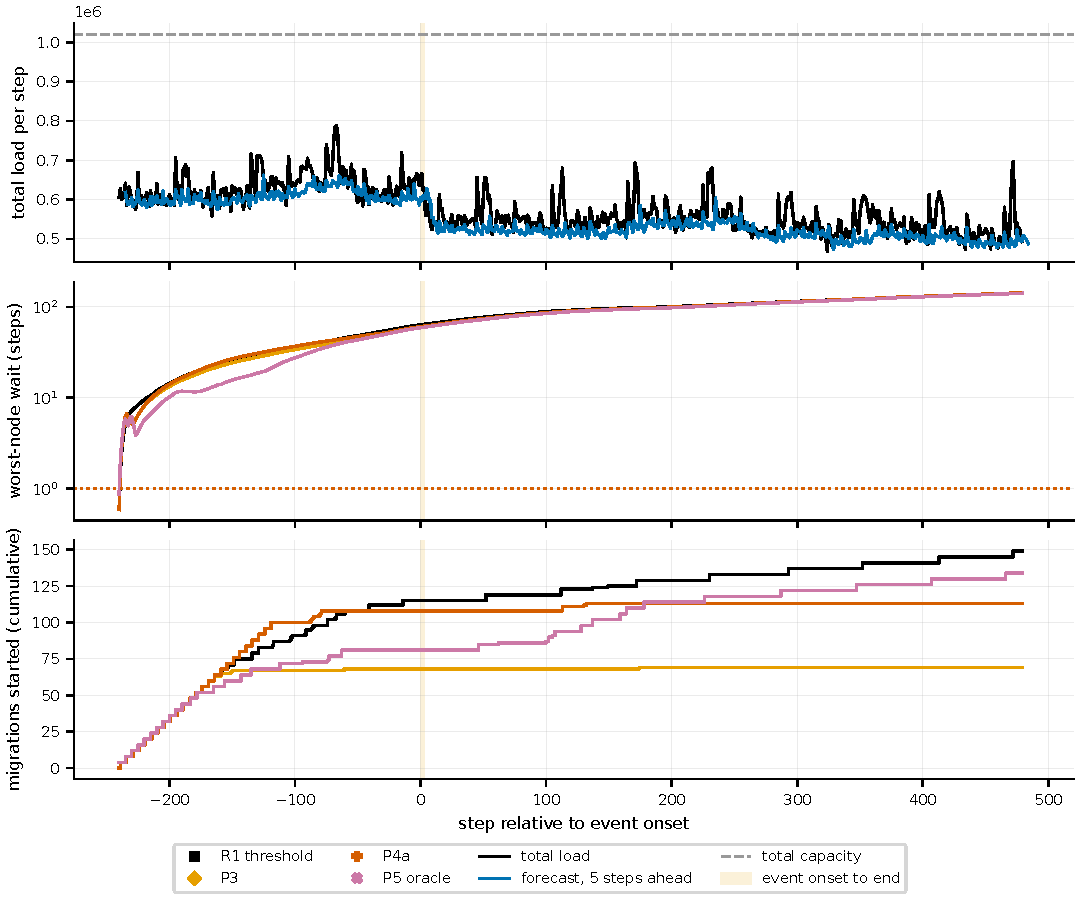
\includegraphics[width=\linewidth]{assets/figures/fa2_episode_D1.pdf}
\caption{FA2 and review Figure 3. Regenerated flash-crowd episode on D1: event D1-5320 (peak 1044), replicate 23. One replicate selected by a rule fixed beforehand, not an average, no interval. Rule: among the 30 sampled abrupt evaluation events of the default cell (m 5, headroom 1.6) the event with the median peak (lower middle on an even count, ties by event id), with the replicate index it has in the frozen rows. Top: total offered load per step, total node capacity and the point forecast of the P4 forecaster (lightgbm), summed over partitions, for the horizon of 5 steps (the default migration duration), the forecast made at step i drawn at its target step i + 5; P3 and P4a act on forecasts of this forecaster and P4a adds an interval margin that is not drawn; the shaded span runs from event onset to end. Middle: worst-node wait proxy in steps (symlog axis, SLO threshold 1 dotted). Bottom: migrations started, cumulative. Policies R1 (P1), P3 (forecaster of P4), P4a, P5. The regenerated damage and number of moves of every drawn policy equal the frozen rows (damage: R1 threshold 12.4552; P3 18.129; P4a 14.3718; P5 oracle 11.8953). Window 720 steps of 60 s, master\_seed 42. Sources: results\_frozen Must rows (P1, P3, P5) and Q1 AA6 rows (P4a), regenerated with the frozen code and configs; table of the comparison: figures/fa2\_episode\_check.csv.}\label{fig:fa2_episode_d1}
\end{figure}

% generated by build_assets.py from the recorded PDF and caption; do not edit
\begin{figure}[tbp]
\centering
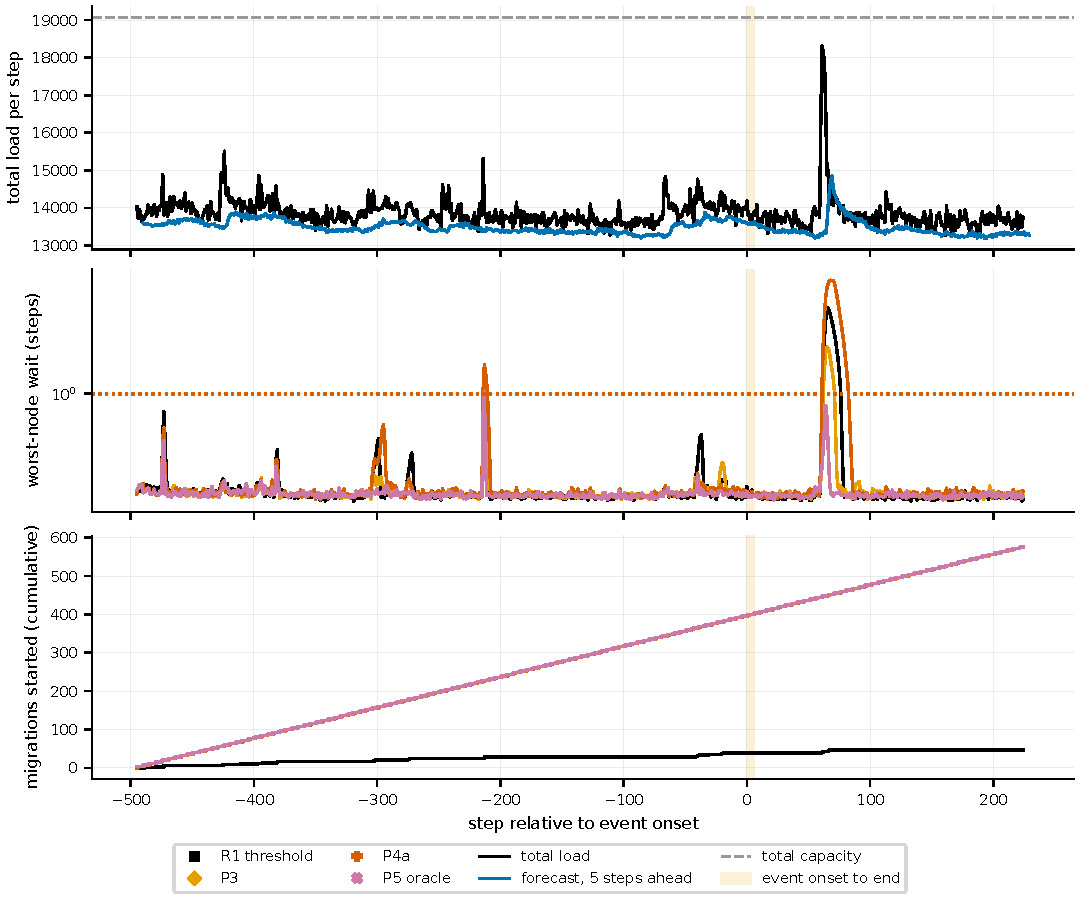
\includegraphics[width=\linewidth]{assets/figures/fa2_episode_D2.pdf}
\caption{FA2 and review Figure 3. Regenerated flash-crowd episode on D2: event D2-122 (peak 175), replicate 22. One replicate selected by a rule fixed beforehand, not an average, no interval. Rule: among the 30 sampled abrupt evaluation events of the default cell (m 5, headroom 1.6) the event with the median peak (lower middle on an even count, ties by event id), with the replicate index it has in the frozen rows. Top: total offered load per step, total node capacity and the point forecast of the P4 forecaster (lightgbm), summed over partitions, for the horizon of 5 steps (the default migration duration), the forecast made at step i drawn at its target step i + 5; P3 and P4a act on forecasts of this forecaster and P4a adds an interval margin that is not drawn; the shaded span runs from event onset to end. Middle: worst-node wait proxy in steps (symlog axis, SLO threshold 1 dotted). Bottom: migrations started, cumulative. Policies R1 (P1), P3 (forecaster of P4), P4a, P5. The regenerated damage and number of moves of every drawn policy equal the frozen rows (damage: R1 threshold 0.00330456; P3 0.00102777; P4a 0.00609227; P5 oracle 2.76524e-06). Window 720 steps of 10 s, master\_seed 42. Sources: results\_frozen Must rows (P1, P3, P5) and Q1 AA6 rows (P4a), regenerated with the frozen code and configs; table of the comparison: figures/fa2\_episode\_check.csv.}\label{fig:fa2_episode_d2}
\end{figure}

% generated by build_assets.py from the recorded PDF and caption; do not edit
\begin{figure}[tbp]
\centering
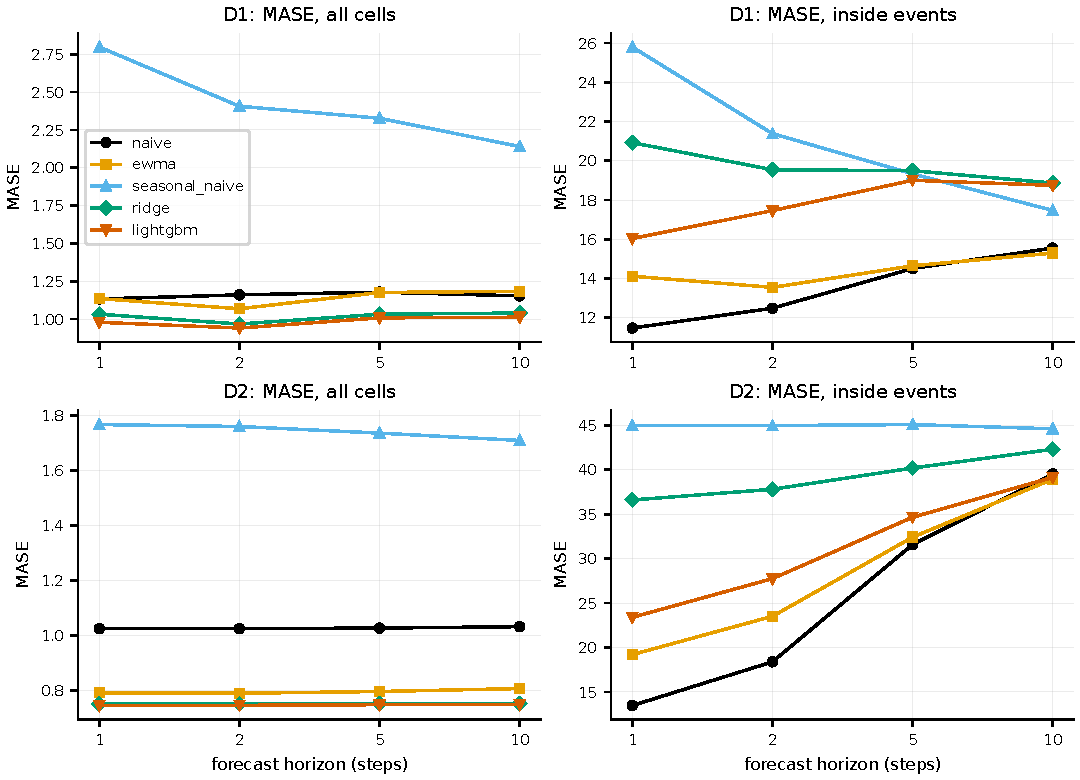
\includegraphics[width=\linewidth]{assets/figures/fa3_forecast_accuracy.pdf}
\caption{FA3. Forecast accuracy on the evaluation split, MASE over all cells and inside events, by forecaster and horizon, per dataset (D1, D2). Values are pooled point estimates from tables/forecast\_accuracy.csv; no interval is drawn because the table holds none. MASE is scaled by the training-prefix naive error, so 1 equals that scale. Source rows are rolling-refit forecasts; the stride-4 Chronos subset is not drawn (see tables/forecast\_accuracy\_chronos.csv). Seed: forecasts are deterministic given the stored tables (master seed 42).}\label{fig:fa3_forecast_accuracy}
\end{figure}

% generated by build_assets.py from the recorded PDF and caption; do not edit
\begin{figure}[tbp]
\centering
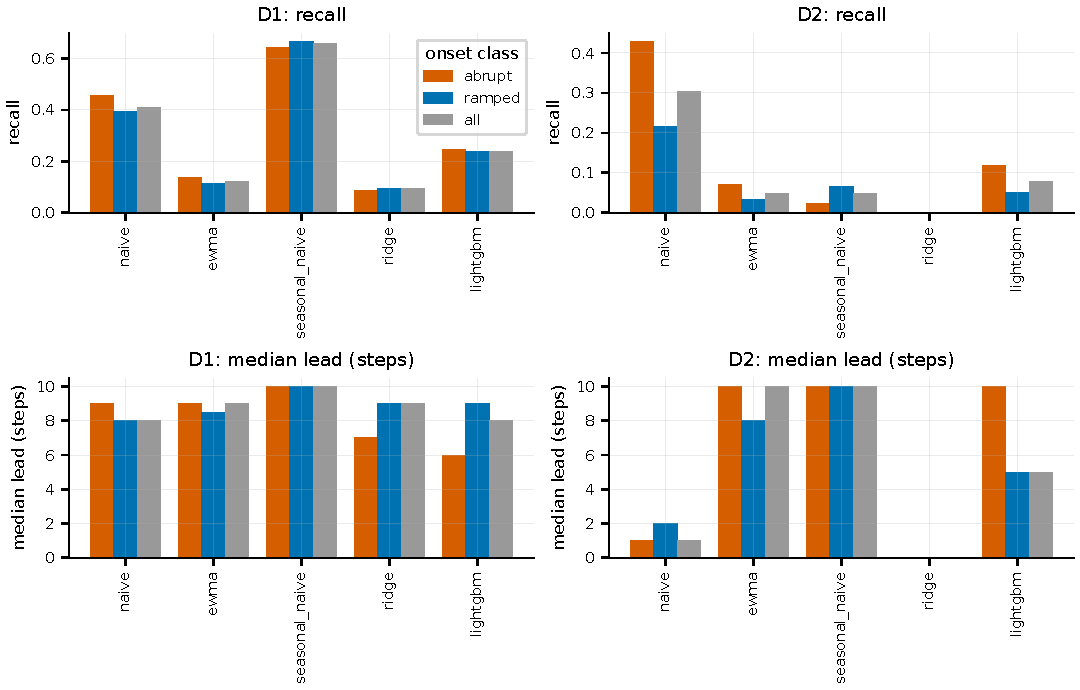
\includegraphics[width=\linewidth]{assets/figures/fa4_early_warning.pdf}
\caption{FA4. Early warning on the evaluation split: recall and median lead time (steps) of each forecaster by onset class, per dataset. Pooled point values from tables/forecast\_accuracy\_early\_warning.csv, no interval in the table. Events per class (naive row, after exclusions; other forecasters differ by the excluded events listed in the table): D1 all 3679; D1 abrupt 957; D1 ramped 2722; D2 all 102; D2 abrupt 42; D2 ramped 60. A missing bar means the value is undefined (no alarm raised). Precision is in the table and is not drawn.}\label{fig:fa4_early_warning}
\end{figure}

% generated by build_assets.py from the recorded PDF and caption; do not edit
\begin{figure}[tbp]
\centering
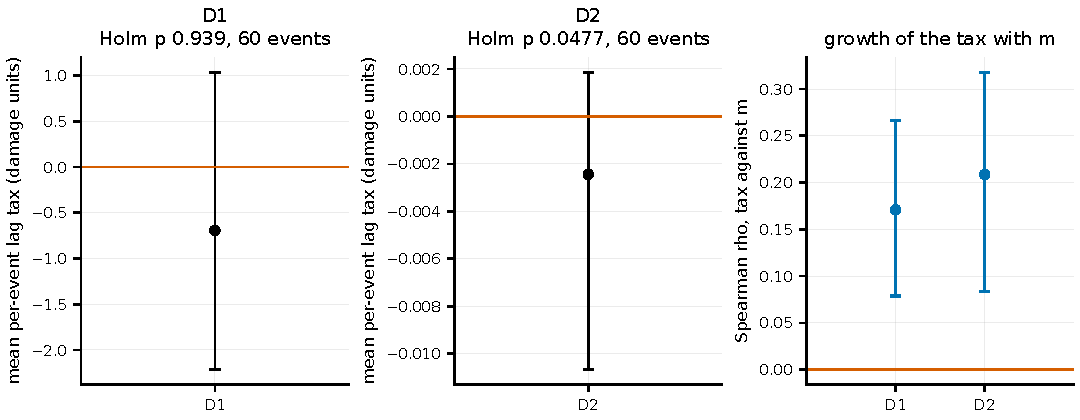
\includegraphics[width=\linewidth]{assets/figures/fa5_lag_tax.pdf}
\caption{FA5. Lag tax (reactive minus oracle damage) per event at the default m and headroom: mean with its 95\% BCa interval over events (9999 resamples, master seed 42) (left, per dataset, own axis because D1 and D2 damage scales differ), and Spearman rho of tax against m (right). Zero line marks no tax. 60 events per dataset; labels and Holm-adjusted p values are those of tables/c1\_lag\_tax.csv (family F1, 4 p values). Hypothesis labels are in the ledger.}\label{fig:fa5_lag_tax}
\end{figure}

% generated by build_assets.py from the recorded PDF and caption; do not edit
\begin{figure}[tbp]
\centering
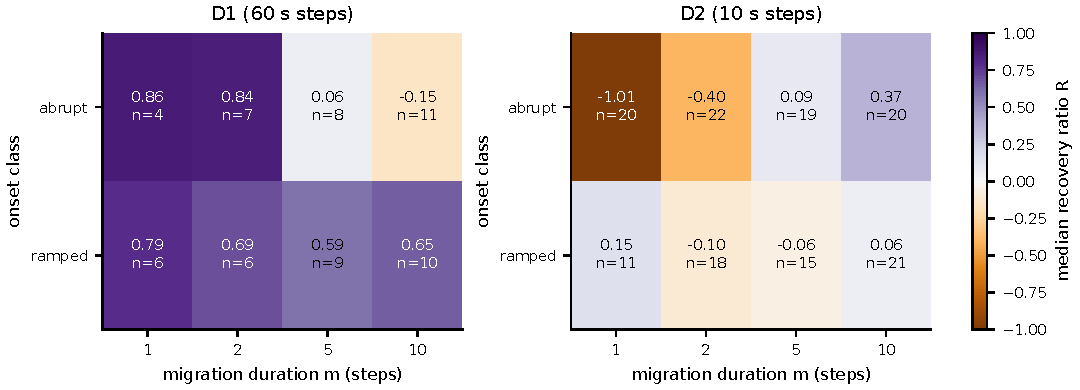
\includegraphics[width=\linewidth]{assets/figures/fa6_regime_must.pdf}
\caption{FA6b. Headline regime map on the real traces: median recovery ratio R of P3\_lightgbm by migration duration m and onset class at headroom 1.6, per dataset. Cell text is the median R over events with R defined and the number n of those events; blank cells have no event with R defined. Colour clipped to -1 to 1. Intervals and the share of replicates with R defined are in tables/regime\_map\_must.csv. Datasets are not pooled.}\label{fig:fa6_regime_must}
\end{figure}

% generated by build_assets.py from the recorded PDF and caption; do not edit
\begin{figure}[tbp]
\centering
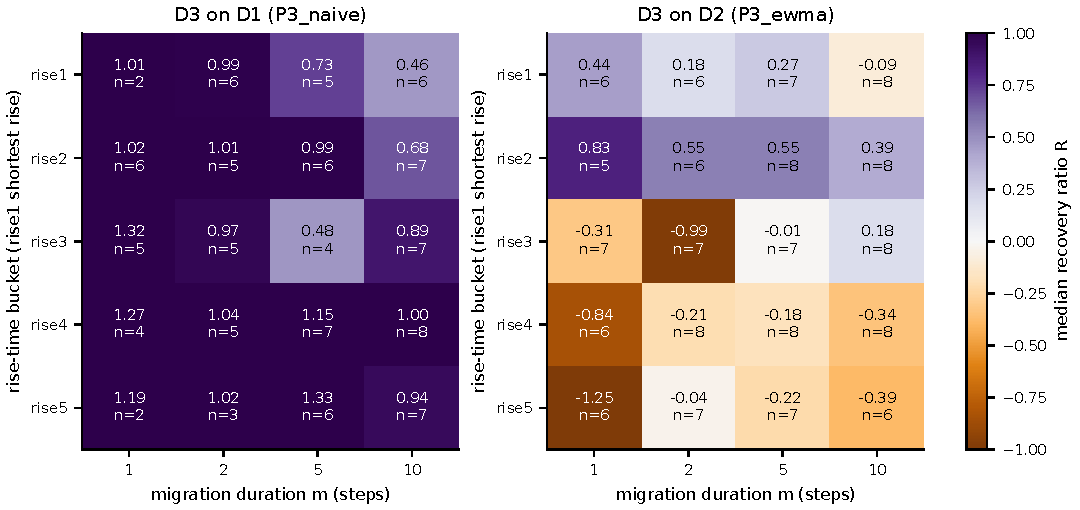
\includegraphics[width=\linewidth]{assets/figures/fa6_regime_q2.pdf}
\caption{FA6a. Measured lag-tax recovery ratio R across migration duration m (x) and flash-crowd rise-time bucket (y), headroom 1.6, injected-event data D3 on D1 and on D2 (forecast policy: P3\_ewma/P3\_naive). Cell text is the median R over events with R defined and the number n of those events (of 8 events per bucket); blank cells have no event with R defined. Colour is clipped to the range -1 to 1, the printed value is not clipped. R is defined only where the lag tax is at least the registered share of the reactive damage. Every cell rests on few events (flag in tables/regime\_map\_q2.csv); intervals are in the table. Datasets are not pooled.}\label{fig:fa6_regime_q2}
\end{figure}

% generated by build_assets.py from the recorded PDF and caption; do not edit
\begin{figure}[tbp]
\centering
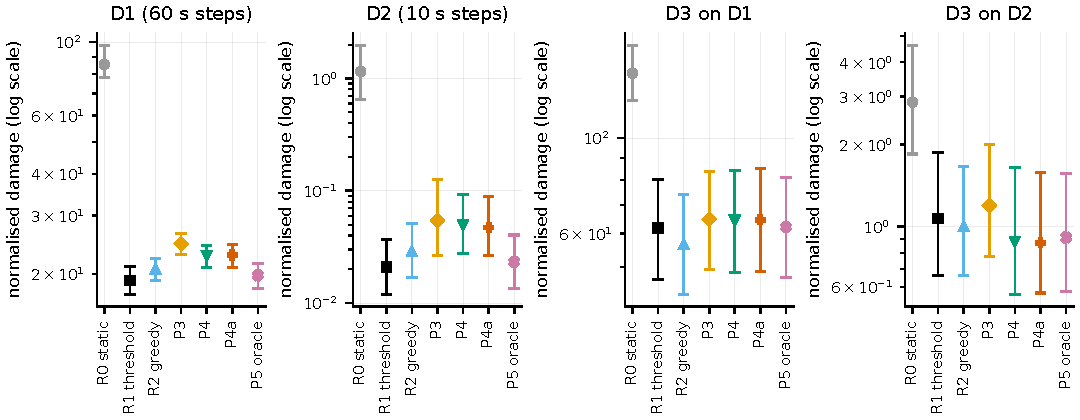
\includegraphics[width=\linewidth]{assets/figures/fa7_damage.pdf}
\caption{FA7a. Overall performance of the seven placement policies: mean per-event normalised damage with its 95\% BCa interval over events (9999 resamples, master seed 42), per dataset (log y axis, each panel its own scale; datasets are not pooled because D1 damage is about 20 and D2 about 0.02). R0, R1 and R2 are P0, P1 and P2. Events per dataset: D1 60; D2 60; D1\_D3 40; D2\_D3 40. Default m and headroom, 30 replicates per event, tables/rt\_policy\_metrics.csv (descriptive, not pre-registered).}\label{fig:fa7_damage}
\end{figure}

% generated by build_assets.py from the recorded PDF and caption; do not edit
\begin{figure}[tbp]
\centering
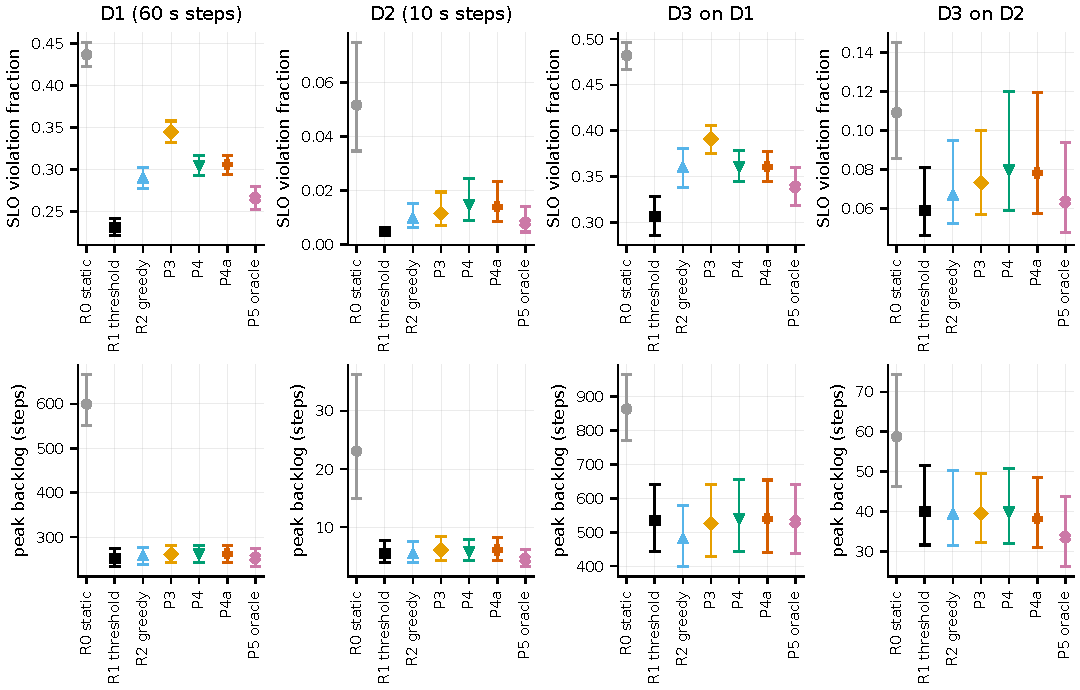
\includegraphics[width=\linewidth]{assets/figures/fa7_violation_backlog.pdf}
\caption{FA7b. SLO violation fraction (top) and peak backlog in steps (bottom) for the seven policies, per dataset: mean per-event value with its 95\% BCa interval over events (9999 resamples, master seed 42). R0, R1, R2 are P0, P1, P2. Events per dataset: D1 60; D2 60; D1\_D3 40; D2\_D3 40. Default m and headroom; tables/rt\_policy\_metrics.csv (descriptive, not pre-registered).}\label{fig:fa7_violation_backlog}
\end{figure}

% generated by build_assets.py from the recorded PDF and caption; do not edit
\begin{figure}[tbp]
\centering
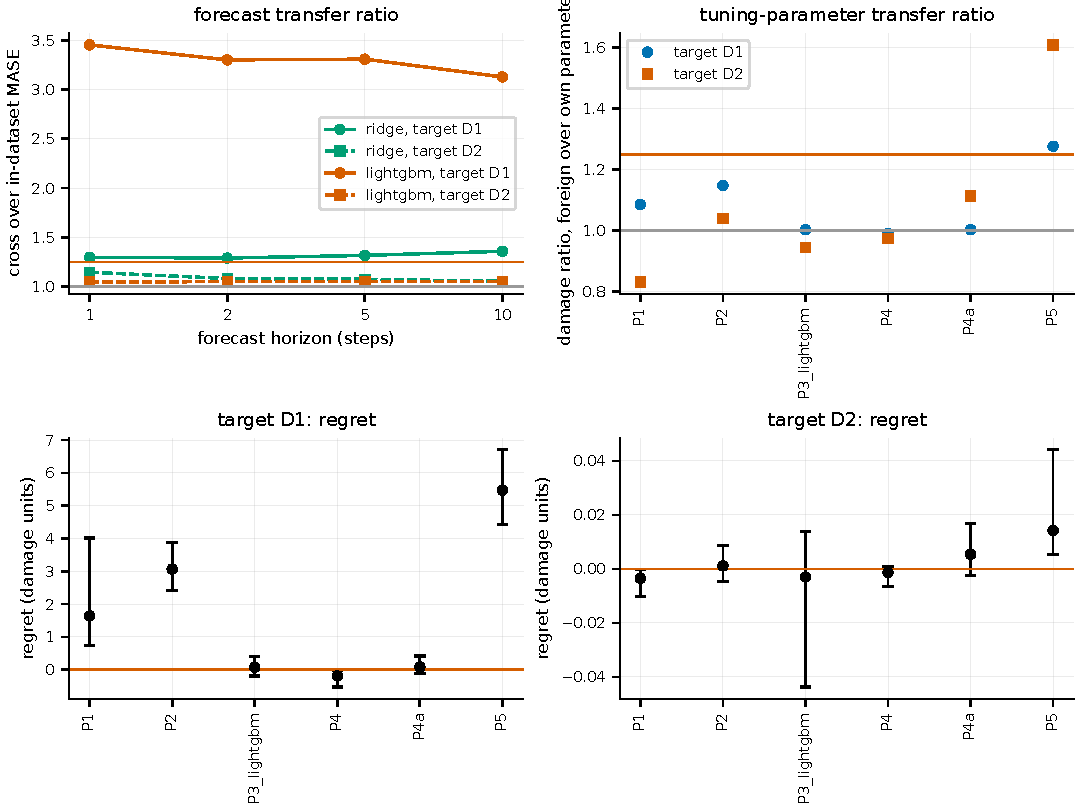
\includegraphics[width=\linewidth]{assets/figures/fa8_transfer.pdf}
\caption{FA8. Cross-dataset transfer. Top left: forecast transfer ratio (fixed model fitted on the source training prefix, scored on the target, over the same protocol in-dataset), ridge and lightgbm, by horizon and target. Top right: tuning-parameter transfer ratio of mean per-event damage, foreign over own parameters, per policy and target. Lines: 1 (grey) and the registered threshold 1.25 (orange). Bottom: regret (foreign minus own mean damage) with 95\% BCa interval over events (9999 resamples, master seed 42), per target on its own damage scale. Source: tables/c5\_transfer\_detail.csv; ratios have no interval in the table.}\label{fig:fa8_transfer}
\end{figure}

% generated by build_assets.py from the recorded PDF and caption; do not edit
\begin{figure}[tbp]
\centering
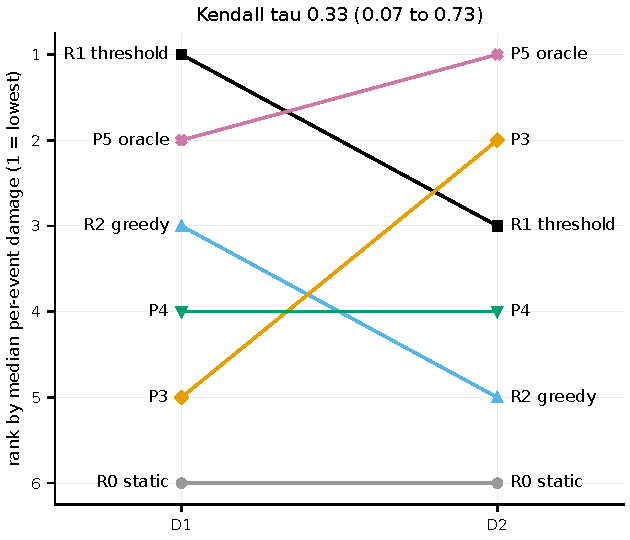
\includegraphics[width=\linewidth]{assets/figures/fa9_ranking.pdf}
\caption{FA9. Policy ranking on D1 and D2 by median per-event damage (60 events on D1, 60 on D2), rank 1 is the lowest damage. R0, R1, R2 are P0, P1, P2. Kendall tau between the two rankings, tau and its percentile bootstrap interval are in the title (6 policies, threshold 0.6 in tables/c6\_ranking\_tau.csv). Source: tables/c6\_ranking.csv.}\label{fig:fa9_ranking}
\end{figure}

% generated by build_assets.py from the recorded PDF and caption; do not edit
\begin{figure}[tbp]
\centering
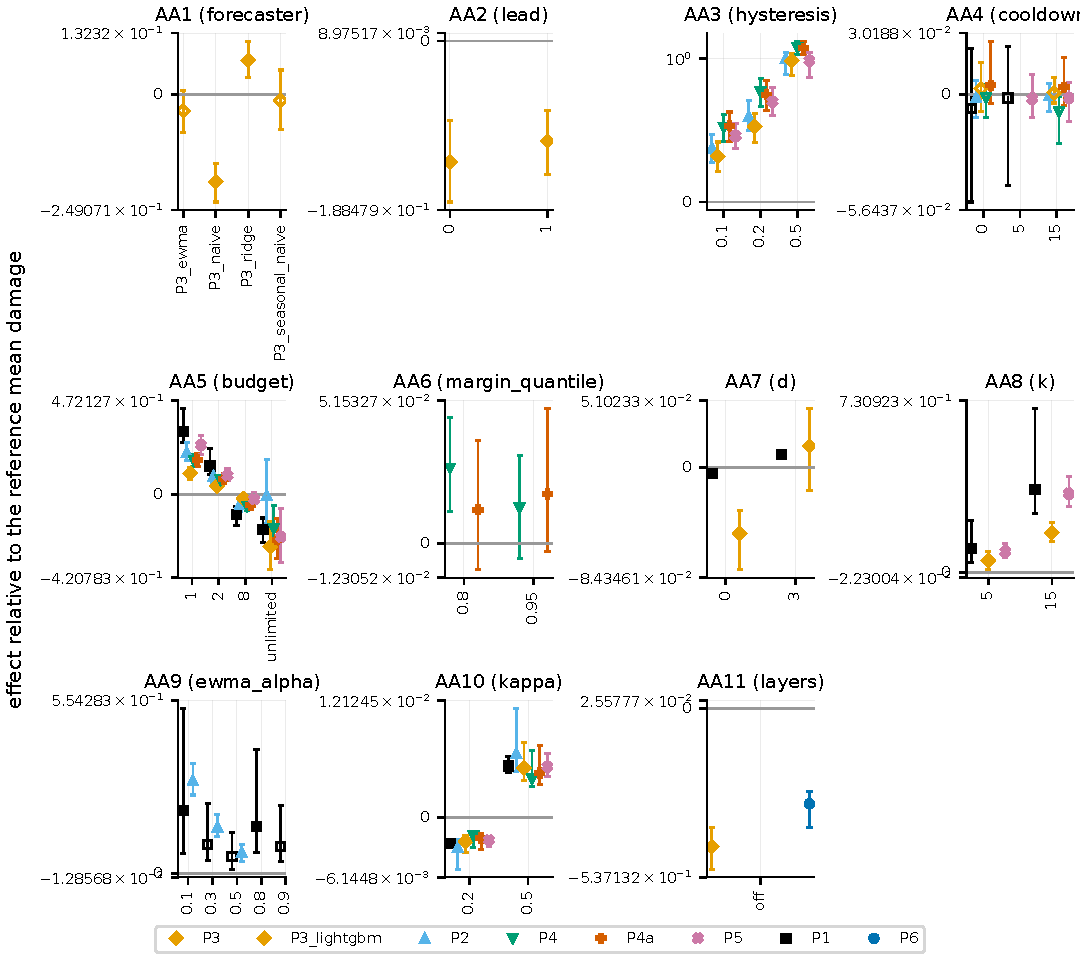
\includegraphics[width=\linewidth]{assets/figures/fa10_ablations_D1.pdf}
\caption{FA10 (D1). Ablation effects on mean per-event damage, level minus reference, as a multiple of the reference mean (symlog axis; 0 means no change, 1 means +100 percent), per ablation AA1 to AA11 and policy, with 95\% BCa interval over events (9999 resamples, master seed 42) over 60 events scaled by the reference mean. Filled markers: Holm-adjusted p below the registered alpha within the ablation; open markers: not. One factor at a time, levels not re-tuned; interactions untested; AA13, XA6 and FA16 were not completed. Source: tables/aa\_ablations.csv (descriptive, no hypothesis label).}\label{fig:fa10_ablations_d1}
\end{figure}

% generated by build_assets.py from the recorded PDF and caption; do not edit
\begin{figure}[tbp]
\centering
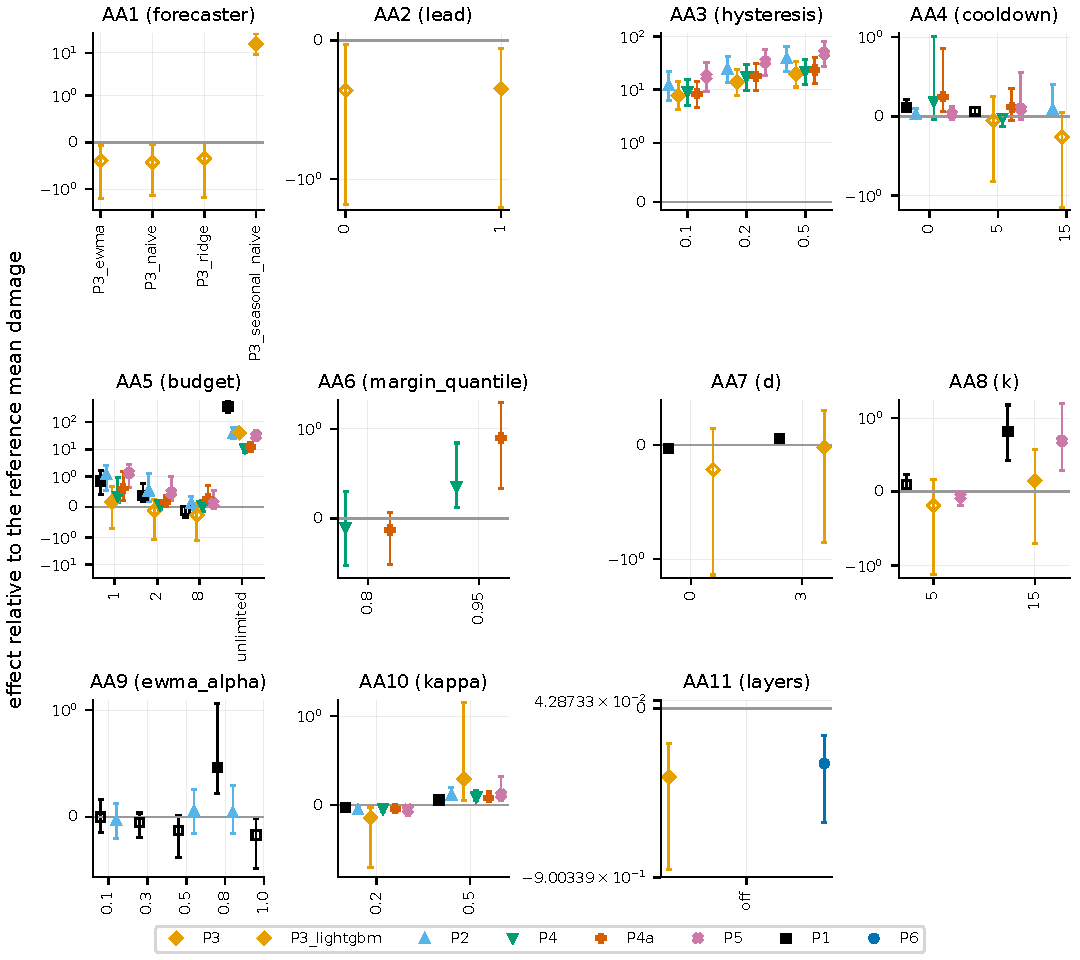
\includegraphics[width=\linewidth]{assets/figures/fa10_ablations_D2.pdf}
\caption{FA10 (D2). Ablation effects on mean per-event damage, level minus reference, as a multiple of the reference mean (symlog axis; 0 means no change, 1 means +100 percent), per ablation AA1 to AA11 and policy, with 95\% BCa interval over events (9999 resamples, master seed 42) over 60 events scaled by the reference mean. Filled markers: Holm-adjusted p below the registered alpha within the ablation; open markers: not. One factor at a time, levels not re-tuned; interactions untested; AA13, XA6 and FA16 were not completed. Source: tables/aa\_ablations.csv (descriptive, no hypothesis label).}\label{fig:fa10_ablations_d2}
\end{figure}

% generated by build_assets.py from the recorded PDF and caption; do not edit
\begin{figure}[tbp]
\centering
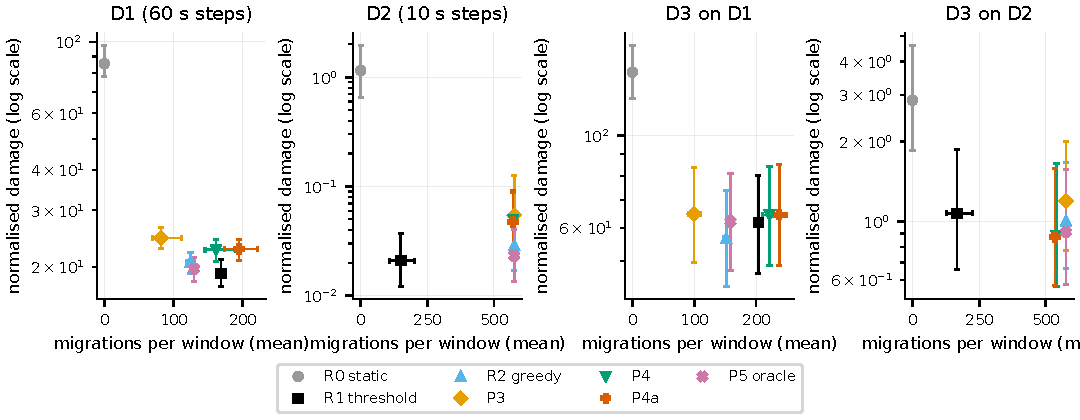
\includegraphics[width=\linewidth]{assets/figures/fa11_damage_moves.pdf}
\caption{FA11. Damage against migration count per policy, per dataset (each panel its own damage scale): mean per-event value with its 95\% BCa interval over events (9999 resamples, master seed 42) on both axes. R0, R1, R2 are P0, P1, P2; R0 never migrates. Events per dataset: D1 60; D2 60; D1\_D3 40; D2\_D3 40. Default m and headroom; tables/rt\_policy\_metrics.csv (descriptive, not pre-registered).}\label{fig:fa11_damage_moves}
\end{figure}

% generated by build_assets.py from the recorded PDF and caption; do not edit
\begin{figure}[tbp]
\centering
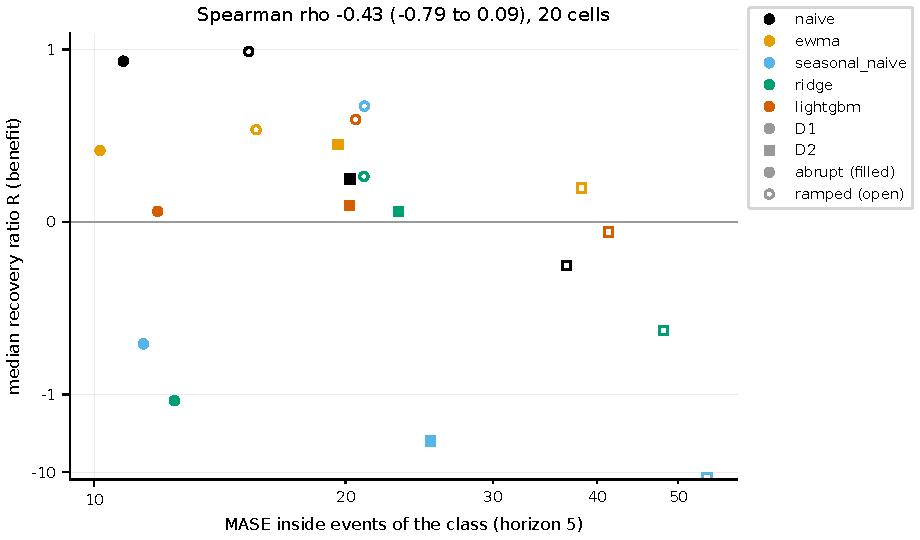
\includegraphics[width=\linewidth]{assets/figures/fa12_mase_benefit.pdf}
\caption{FA12. Forecast accuracy against control benefit: one point per cell (forecaster, dataset, onset class), x is the MASE inside events of that class at the horizon nearest m plus d, y is the cell median recovery ratio R. Circles: D1, squares: D2; filled: abrupt, open: ramped. Spearman rho with its 95\% BCa interval over events (9999 resamples, master seed 42) over cells is in the title (exploratory p 0.0594); cell benefits rest on the events with R defined (8 to 19 per cell, tables/c4\_accuracy\_benefit\_cells.csv). Symlog y axis.}\label{fig:fa12_mase_benefit}
\end{figure}

% generated by build_assets.py from the recorded PDF and caption; do not edit
\begin{figure}[tbp]
\centering
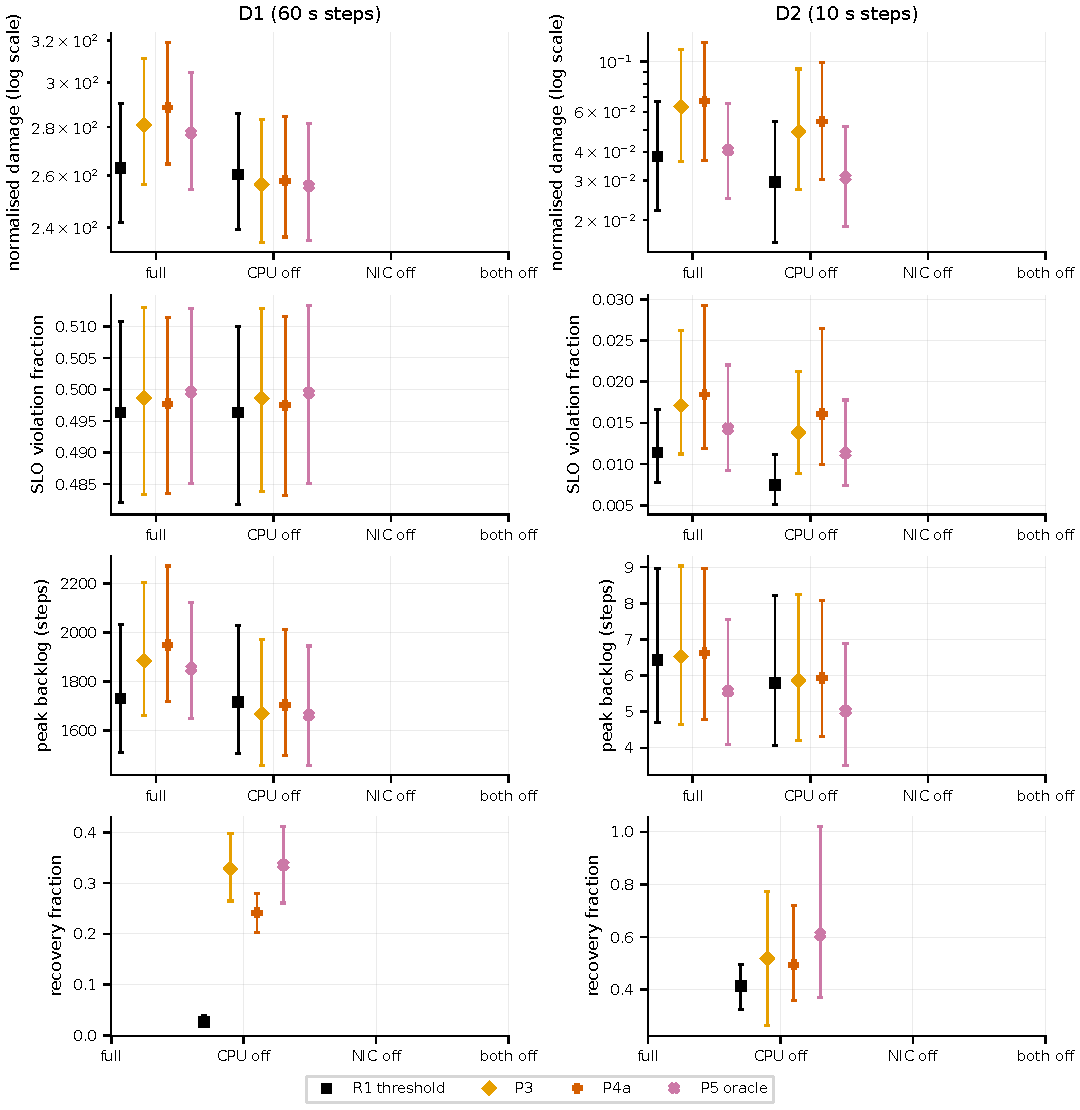
\includegraphics[width=\linewidth]{assets/figures/fa13_contention.pdf}
\caption{FA13. Contention ablation (RV1) in the coupled model, per dataset (each panel its own scale): mean per-event damage (log scale), SLO violation fraction and peak backlog with their 95\% BCa interval over events (9999 resamples, master seed 42), and the recovery fraction of tables/rv1\_contention.csv (bottom row; blank where it is undefined, which includes the full model, the reference). Levels: full model, CPU contention off, NIC contention off, both off. The constant-m control mode is in the tables and not drawn. Events per dataset: D1 60; D2 60. Tables: tables/rt\_rv1\_metrics.csv (descriptive, not pre-registered) and tables/rv1\_contention.csv.}\label{fig:fa13_contention}
\end{figure}

% generated by build_assets.py from the recorded PDF and caption; do not edit
\begin{figure}[tbp]
\centering
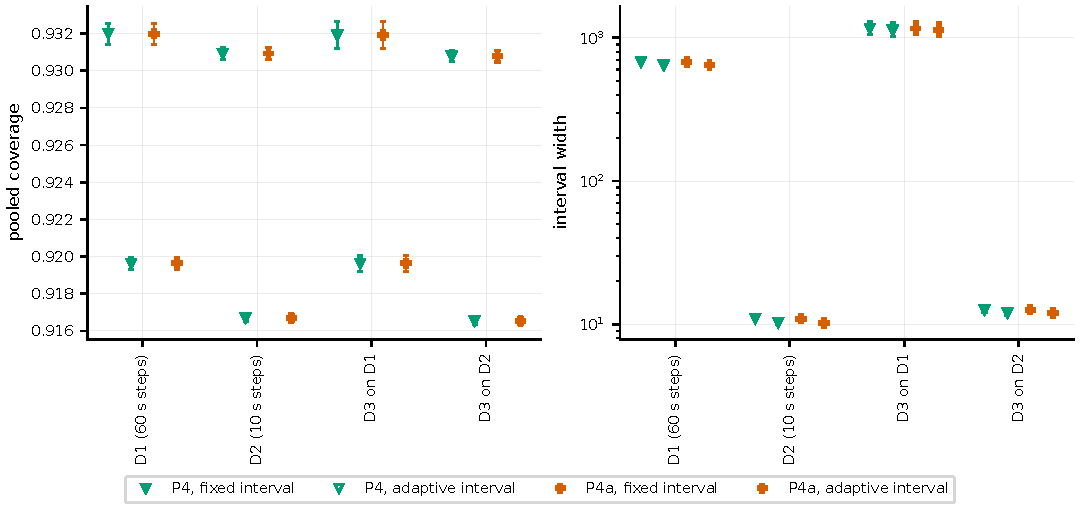
\includegraphics[width=\linewidth]{assets/figures/fa14_conformal_logging.pdf}
\caption{FA14. Conformal interval logging (RV4): pooled coverage (left) and interval width (right, log scale) of the fixed and the adaptive interval, for P4 and P4a, per dataset (widths are not comparable across datasets). Filled markers: fixed interval; open: adaptive. Mean with its 95\% BCa interval over events (9999 resamples, master seed 42). The table holds pooled values, so there is no time axis; the adaptive level (alpha), the point error and the trigger counts are in the table and not drawn. Events per dataset: D1 60; D2 60; D1\_D3 40; D2\_D3 40. Source: tables/rv4\_logging.csv.}\label{fig:fa14_conformal_logging}
\end{figure}

% generated by build_assets.py from the recorded PDF and caption; do not edit
\begin{figure}[tbp]
\centering
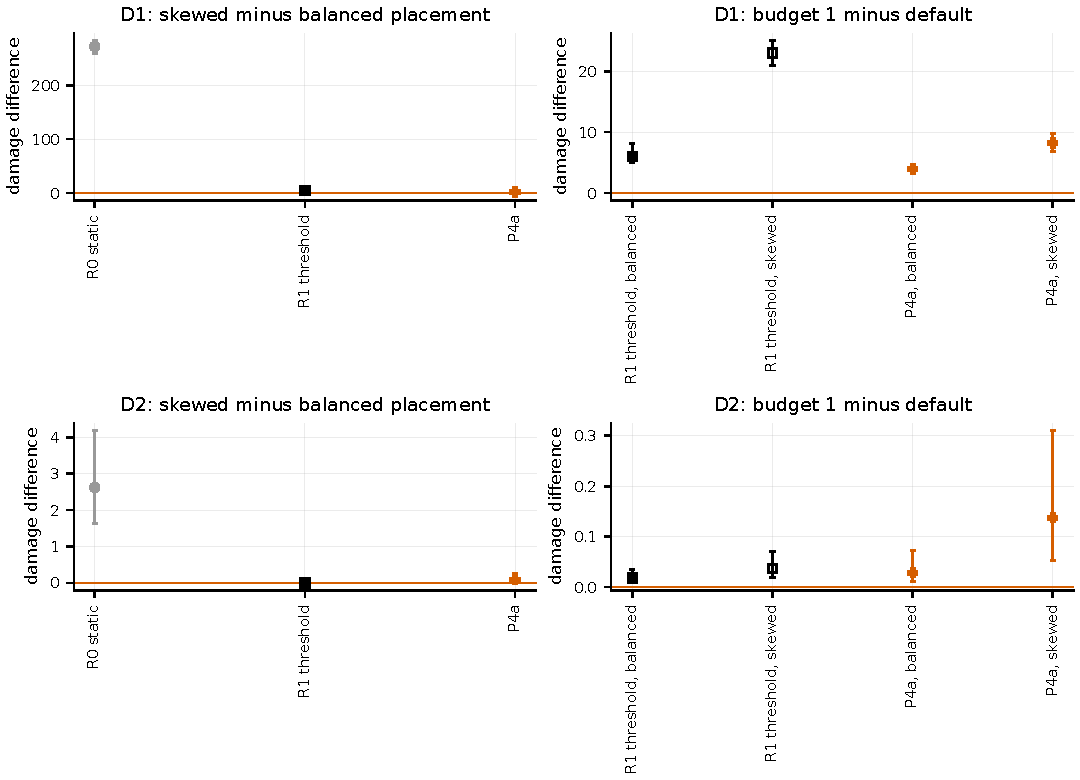
\includegraphics[width=\linewidth]{assets/figures/fa15_placement_budget.pdf}
\caption{FA15. Placement and migration budget (RV2, RV3), per dataset (each panel its own damage scale). Left: mean per-event damage under skewed placement minus balanced placement, for R0, R1 and P4a. Right: mean per-event damage with migration budget 1 minus the default budget, for R1 and P4a, under balanced placement (filled) and skewed placement (open). Mean difference with its 95\% BCa interval over events (9999 resamples, master seed 42); zero line marks no difference. R0, R1 are P0, P1. Events per dataset: D1 60; D2 60. Sources: tables/rv2\_placement.csv and tables/rv3\_budget.csv. Review figure 10 asked for the throttled policy; the recorded RV3 rows hold the budget-1 contrast, which is what is drawn.}\label{fig:fa15_placement_budget}
\end{figure}

